% Options for packages loaded elsewhere
\PassOptionsToPackage{unicode}{hyperref}
\PassOptionsToPackage{hyphens}{url}
\PassOptionsToPackage{dvipsnames,svgnames,x11names}{xcolor}
%
\documentclass[
  letterpaper,
  DIV=11,
  numbers=noendperiod]{scrreprt}

\usepackage{amsmath,amssymb}
\usepackage{iftex}
\ifPDFTeX
  \usepackage[T1]{fontenc}
  \usepackage[utf8]{inputenc}
  \usepackage{textcomp} % provide euro and other symbols
\else % if luatex or xetex
  \usepackage{unicode-math}
  \defaultfontfeatures{Scale=MatchLowercase}
  \defaultfontfeatures[\rmfamily]{Ligatures=TeX,Scale=1}
\fi
\usepackage{lmodern}
\ifPDFTeX\else  
    % xetex/luatex font selection
\fi
% Use upquote if available, for straight quotes in verbatim environments
\IfFileExists{upquote.sty}{\usepackage{upquote}}{}
\IfFileExists{microtype.sty}{% use microtype if available
  \usepackage[]{microtype}
  \UseMicrotypeSet[protrusion]{basicmath} % disable protrusion for tt fonts
}{}
\makeatletter
\@ifundefined{KOMAClassName}{% if non-KOMA class
  \IfFileExists{parskip.sty}{%
    \usepackage{parskip}
  }{% else
    \setlength{\parindent}{0pt}
    \setlength{\parskip}{6pt plus 2pt minus 1pt}}
}{% if KOMA class
  \KOMAoptions{parskip=half}}
\makeatother
\usepackage{xcolor}
\setlength{\emergencystretch}{3em} % prevent overfull lines
\setcounter{secnumdepth}{5}
% Make \paragraph and \subparagraph free-standing
\ifx\paragraph\undefined\else
  \let\oldparagraph\paragraph
  \renewcommand{\paragraph}[1]{\oldparagraph{#1}\mbox{}}
\fi
\ifx\subparagraph\undefined\else
  \let\oldsubparagraph\subparagraph
  \renewcommand{\subparagraph}[1]{\oldsubparagraph{#1}\mbox{}}
\fi

\usepackage{color}
\usepackage{fancyvrb}
\newcommand{\VerbBar}{|}
\newcommand{\VERB}{\Verb[commandchars=\\\{\}]}
\DefineVerbatimEnvironment{Highlighting}{Verbatim}{commandchars=\\\{\}}
% Add ',fontsize=\small' for more characters per line
\usepackage{framed}
\definecolor{shadecolor}{RGB}{241,243,245}
\newenvironment{Shaded}{\begin{snugshade}}{\end{snugshade}}
\newcommand{\AlertTok}[1]{\textcolor[rgb]{0.68,0.00,0.00}{#1}}
\newcommand{\AnnotationTok}[1]{\textcolor[rgb]{0.37,0.37,0.37}{#1}}
\newcommand{\AttributeTok}[1]{\textcolor[rgb]{0.40,0.45,0.13}{#1}}
\newcommand{\BaseNTok}[1]{\textcolor[rgb]{0.68,0.00,0.00}{#1}}
\newcommand{\BuiltInTok}[1]{\textcolor[rgb]{0.00,0.23,0.31}{#1}}
\newcommand{\CharTok}[1]{\textcolor[rgb]{0.13,0.47,0.30}{#1}}
\newcommand{\CommentTok}[1]{\textcolor[rgb]{0.37,0.37,0.37}{#1}}
\newcommand{\CommentVarTok}[1]{\textcolor[rgb]{0.37,0.37,0.37}{\textit{#1}}}
\newcommand{\ConstantTok}[1]{\textcolor[rgb]{0.56,0.35,0.01}{#1}}
\newcommand{\ControlFlowTok}[1]{\textcolor[rgb]{0.00,0.23,0.31}{#1}}
\newcommand{\DataTypeTok}[1]{\textcolor[rgb]{0.68,0.00,0.00}{#1}}
\newcommand{\DecValTok}[1]{\textcolor[rgb]{0.68,0.00,0.00}{#1}}
\newcommand{\DocumentationTok}[1]{\textcolor[rgb]{0.37,0.37,0.37}{\textit{#1}}}
\newcommand{\ErrorTok}[1]{\textcolor[rgb]{0.68,0.00,0.00}{#1}}
\newcommand{\ExtensionTok}[1]{\textcolor[rgb]{0.00,0.23,0.31}{#1}}
\newcommand{\FloatTok}[1]{\textcolor[rgb]{0.68,0.00,0.00}{#1}}
\newcommand{\FunctionTok}[1]{\textcolor[rgb]{0.28,0.35,0.67}{#1}}
\newcommand{\ImportTok}[1]{\textcolor[rgb]{0.00,0.46,0.62}{#1}}
\newcommand{\InformationTok}[1]{\textcolor[rgb]{0.37,0.37,0.37}{#1}}
\newcommand{\KeywordTok}[1]{\textcolor[rgb]{0.00,0.23,0.31}{#1}}
\newcommand{\NormalTok}[1]{\textcolor[rgb]{0.00,0.23,0.31}{#1}}
\newcommand{\OperatorTok}[1]{\textcolor[rgb]{0.37,0.37,0.37}{#1}}
\newcommand{\OtherTok}[1]{\textcolor[rgb]{0.00,0.23,0.31}{#1}}
\newcommand{\PreprocessorTok}[1]{\textcolor[rgb]{0.68,0.00,0.00}{#1}}
\newcommand{\RegionMarkerTok}[1]{\textcolor[rgb]{0.00,0.23,0.31}{#1}}
\newcommand{\SpecialCharTok}[1]{\textcolor[rgb]{0.37,0.37,0.37}{#1}}
\newcommand{\SpecialStringTok}[1]{\textcolor[rgb]{0.13,0.47,0.30}{#1}}
\newcommand{\StringTok}[1]{\textcolor[rgb]{0.13,0.47,0.30}{#1}}
\newcommand{\VariableTok}[1]{\textcolor[rgb]{0.07,0.07,0.07}{#1}}
\newcommand{\VerbatimStringTok}[1]{\textcolor[rgb]{0.13,0.47,0.30}{#1}}
\newcommand{\WarningTok}[1]{\textcolor[rgb]{0.37,0.37,0.37}{\textit{#1}}}

\providecommand{\tightlist}{%
  \setlength{\itemsep}{0pt}\setlength{\parskip}{0pt}}\usepackage{longtable,booktabs,array}
\usepackage{multirow}
\usepackage{calc} % for calculating minipage widths
% Correct order of tables after \paragraph or \subparagraph
\usepackage{etoolbox}
\makeatletter
\patchcmd\longtable{\par}{\if@noskipsec\mbox{}\fi\par}{}{}
\makeatother
% Allow footnotes in longtable head/foot
\IfFileExists{footnotehyper.sty}{\usepackage{footnotehyper}}{\usepackage{footnote}}
\makesavenoteenv{longtable}
\usepackage{graphicx}
\makeatletter
\def\maxwidth{\ifdim\Gin@nat@width>\linewidth\linewidth\else\Gin@nat@width\fi}
\def\maxheight{\ifdim\Gin@nat@height>\textheight\textheight\else\Gin@nat@height\fi}
\makeatother
% Scale images if necessary, so that they will not overflow the page
% margins by default, and it is still possible to overwrite the defaults
% using explicit options in \includegraphics[width, height, ...]{}
\setkeys{Gin}{width=\maxwidth,height=\maxheight,keepaspectratio}
% Set default figure placement to htbp
\makeatletter
\def\fps@figure{htbp}
\makeatother

\KOMAoption{captions}{tableheading}
\makeatletter
\@ifpackageloaded{tcolorbox}{}{\usepackage[skins,breakable]{tcolorbox}}
\@ifpackageloaded{fontawesome5}{}{\usepackage{fontawesome5}}
\definecolor{quarto-callout-color}{HTML}{909090}
\definecolor{quarto-callout-note-color}{HTML}{0758E5}
\definecolor{quarto-callout-important-color}{HTML}{CC1914}
\definecolor{quarto-callout-warning-color}{HTML}{EB9113}
\definecolor{quarto-callout-tip-color}{HTML}{00A047}
\definecolor{quarto-callout-caution-color}{HTML}{FC5300}
\definecolor{quarto-callout-color-frame}{HTML}{acacac}
\definecolor{quarto-callout-note-color-frame}{HTML}{4582ec}
\definecolor{quarto-callout-important-color-frame}{HTML}{d9534f}
\definecolor{quarto-callout-warning-color-frame}{HTML}{f0ad4e}
\definecolor{quarto-callout-tip-color-frame}{HTML}{02b875}
\definecolor{quarto-callout-caution-color-frame}{HTML}{fd7e14}
\makeatother
\makeatletter
\makeatother
\makeatletter
\@ifpackageloaded{bookmark}{}{\usepackage{bookmark}}
\makeatother
\makeatletter
\@ifpackageloaded{caption}{}{\usepackage{caption}}
\AtBeginDocument{%
\ifdefined\contentsname
  \renewcommand*\contentsname{Table of contents}
\else
  \newcommand\contentsname{Table of contents}
\fi
\ifdefined\listfigurename
  \renewcommand*\listfigurename{List of Figures}
\else
  \newcommand\listfigurename{List of Figures}
\fi
\ifdefined\listtablename
  \renewcommand*\listtablename{List of Tables}
\else
  \newcommand\listtablename{List of Tables}
\fi
\ifdefined\figurename
  \renewcommand*\figurename{Figure}
\else
  \newcommand\figurename{Figure}
\fi
\ifdefined\tablename
  \renewcommand*\tablename{Table}
\else
  \newcommand\tablename{Table}
\fi
}
\@ifpackageloaded{float}{}{\usepackage{float}}
\floatstyle{ruled}
\@ifundefined{c@chapter}{\newfloat{codelisting}{h}{lop}}{\newfloat{codelisting}{h}{lop}[chapter]}
\floatname{codelisting}{Listing}
\newcommand*\listoflistings{\listof{codelisting}{List of Listings}}
\makeatother
\makeatletter
\@ifpackageloaded{caption}{}{\usepackage{caption}}
\@ifpackageloaded{subcaption}{}{\usepackage{subcaption}}
\makeatother
\makeatletter
\@ifpackageloaded{tcolorbox}{}{\usepackage[skins,breakable]{tcolorbox}}
\makeatother
\makeatletter
\@ifundefined{shadecolor}{\definecolor{shadecolor}{rgb}{.97, .97, .97}}
\makeatother
\makeatletter
\makeatother
\makeatletter
\makeatother
\ifLuaTeX
  \usepackage{selnolig}  % disable illegal ligatures
\fi
\IfFileExists{bookmark.sty}{\usepackage{bookmark}}{\usepackage{hyperref}}
\IfFileExists{xurl.sty}{\usepackage{xurl}}{} % add URL line breaks if available
\urlstyle{same} % disable monospaced font for URLs
\hypersetup{
  pdftitle={写给文科生的Python教程},
  pdfauthor={Weicheng Li},
  colorlinks=true,
  linkcolor={blue},
  filecolor={Maroon},
  citecolor={Blue},
  urlcolor={Blue},
  pdfcreator={LaTeX via pandoc}}

\title{写给文科生的Python教程}
\usepackage{etoolbox}
\makeatletter
\providecommand{\subtitle}[1]{% add subtitle to \maketitle
  \apptocmd{\@title}{\par {\large #1 \par}}{}{}
}
\makeatother
\subtitle{Python for Social Scientists v2.1}
\author{Weicheng Li}
\date{2023-12-20}

\begin{document}
\maketitle
\ifdefined\Shaded\renewenvironment{Shaded}{\begin{tcolorbox}[frame hidden, enhanced, borderline west={3pt}{0pt}{shadecolor}, sharp corners, interior hidden, breakable, boxrule=0pt]}{\end{tcolorbox}}\fi

\renewcommand*\contentsname{Table of contents}
{
\hypersetup{linkcolor=}
\setcounter{tocdepth}{2}
\tableofcontents
}
\bookmarksetup{startatroot}

\hypertarget{ux5f15ux8a00}{%
\chapter*{引言}\label{ux5f15ux8a00}}
\addcontentsline{toc}{chapter}{引言}

\markboth{引言}{引言}

本课程是Python入门、数据处理和分析的教程,适用于经管类本科专业。考虑到同学们的计算机基础可能有比较大的差异,因此本课程也兼有编程入门的性质,在基础部分会讲得详细一些。

\begin{enumerate}
\def\labelenumi{\arabic{enumi}.}
\tightlist
\item
  本课件的网址为\url{https://py4ss.net/python},需要和课程配套使用。这份讲义每年都会有很大的改写,特别是中后段,同时也会根据教学过程逐步更新。
\item
  本课程\textbf{强烈建议}带笔记本电脑上课,并要求在自己的电脑上安装Python环境(后面会有安装教学)。
\item
  Python作为流行的编程语言,网络资料非常丰富。除了跟班学习之外,也推荐充分利用网络资源,比如搜索引擎(不推荐百度,搜索专业类问题结果比较糟糕,能用谷歌最佳,否则也可以考虑用bing),网课或者各种AI工具。
\end{enumerate}

\hypertarget{ux672cux8bfeux7a0bux7684ux4e3bux8981ux5185ux5bb9}{%
\section*{本课程的主要内容:}\label{ux672cux8bfeux7a0bux7684ux4e3bux8981ux5185ux5bb9}}
\addcontentsline{toc}{section}{本课程的主要内容:}

\markright{本课程的主要内容:}

基础部分:

\begin{enumerate}
\def\labelenumi{\arabic{enumi}.}
\tightlist
\item
  Python入门
\item
  基础数据处理、绘图和分析
\item
  基础统计分析、聚类、回归等(重写中)
\end{enumerate}

专业部分:

\begin{enumerate}
\def\labelenumi{\arabic{enumi}.}
\tightlist
\item
  金融类专业48学时版:最优组合、量化技术分析和交易策略初步
\end{enumerate}

其他:看教学情况适时调整。

\hypertarget{ux4e0aux8bfeux5f62ux5f0f}{%
\section*{上课形式}\label{ux4e0aux8bfeux5f62ux5f0f}}
\addcontentsline{toc}{section}{上课形式}

\markright{上课形式}

\begin{enumerate}
\def\labelenumi{\arabic{enumi}.}
\tightlist
\item
  课堂讲解
\item
  ★
  课堂作业:经过初期几次课后,每次课的末尾都会有需要现场完成的编程作业,需要在一定时间内完成并提交,老师公布参考写法,随机抽选几位幸运同学的作业(匿名)来进行解析。
\end{enumerate}

▶ \href{https://py4ss.net/aasp}{课堂作业提交系统}

\hypertarget{ux8003ux5bdfux5f62ux5f0f}{%
\section*{考察形式}\label{ux8003ux5bdfux5f62ux5f0f}}
\addcontentsline{toc}{section}{考察形式}

\markright{考察形式}

\begin{enumerate}
\def\labelenumi{\arabic{enumi}.}
\tightlist
\item
  30\%平时分,70\%期末考察
\item
  期末考察的形式是编程大作业,包括一般性的算法题和专业相关的分析题
\end{enumerate}

\hypertarget{ux8003ux8651ux589eux8865ux7684ux5185ux5bb9}{%
\section*{考虑增补的内容:}\label{ux8003ux8651ux589eux8865ux7684ux5185ux5bb9}}
\addcontentsline{toc}{section}{考虑增补的内容:}

\markright{考虑增补的内容:}

\begin{tcolorbox}[enhanced jigsaw, opacityback=0, left=2mm, coltitle=black, leftrule=.75mm, bottomtitle=1mm, arc=.35mm, opacitybacktitle=0.6, bottomrule=.15mm, breakable, colbacktitle=quarto-callout-warning-color!10!white, toprule=.15mm, toptitle=1mm, colframe=quarto-callout-warning-color-frame, titlerule=0mm, title=\textcolor{quarto-callout-warning-color}{\faExclamationTriangle}\hspace{0.5em}{Warning}, rightrule=.15mm, colback=white]

\begin{enumerate}
\def\labelenumi{\arabic{enumi}.}
\tightlist
\item
  字符串专题 + 正则表达式
\item
  面向对象进阶 + 简单设计模式
\item
  爬虫入门 (技术路线太长)
\item
  (✓) CAPM,最优组合,简单量化交易
\item
  Python操作Excel(非数据部分,包括字体、排版、合并单元格等等)
\item
  更多的案例 (★)
\end{enumerate}

\end{tcolorbox}

\part{第1部分 Python基础}

\hypertarget{ux642dux5efapythonux7f16ux7a0bux73afux5883}{%
\chapter{搭建Python编程环境}\label{ux642dux5efapythonux7f16ux7a0bux73afux5883}}

本课程采用的编程环境是Anaconda + vscode,这也是业界常见的组合。

\hypertarget{ux5b89ux88c5anaconda}{%
\section{安装Anaconda}\label{ux5b89ux88c5anaconda}}

Python除了指代一种编程语言,同时指一个巨大的程序仓库。Python非常流行,因此用Python编程的一个好处,就是你遇到的大部分问题,都有别人写好的程序(称为包Package或者库Library)帮你来完成。

例如,处理二维表格的Pandas,绘图包Matplotlib等等,这些包已经完成了绝大部分基础性的工作,你只要按你的要求调用它们提供的函数或者方法即可。比如你只要告诉Pandas读取一个Excel文件,数据出现在你的屏幕上:从你的指令开始,中间工作都不用你来完成。

大部分编程工作,我们往往要调用大量这些别人写好的包或者库。但是数据分析类的工作,要用的库大同小异,因此有人把面向这类工作的包(包括上述Pandas和Matplotlib等),全部打包到一起,形成一个所谓``发行版'',这就是的Anaconda。

Anaconda包括了Python的执行程序(代码的解释器等)以及大部分数据分析工作要用到的包(虽然大部分你可能用不到),完成本课程有余。

当前(2023年8月),最新版本的Anacoda附带的Python为3.11.x版,我们的课程默认是用这个版本。但需要注意,实际上工作中最新是意见非常危险的事情,往往选择上一个版本(比如3.10.x版)会更加稳妥。

Anaconda的安装包可以在其官方网站下载。如果官方网站访问速度太慢,可以采用清华大学的镜像地址。

安装则只需要一路下一步即可。

注意:安装时请选择``Just Me(仅为我安装)'',而不要选``All Users''。

\hypertarget{ux4e0bux8f7danacondaux5b98ux7f51}{%
\subsection{下载Anaconda(官网)}\label{ux4e0bux8f7danacondaux5b98ux7f51}}

下载地址:https://www.anaconda.com/download\#downloads

拉到最后,按你电脑的操作系统,选择下载对应的64-Bit Graphical
Installer即可。

\hypertarget{ux4e0bux8f7danacondaux6e05ux534eux5927ux5b66ux955cux50cf}{%
\subsection{下载Anaconda(清华大学镜像)}\label{ux4e0bux8f7danacondaux6e05ux534eux5927ux5b66ux955cux50cf}}

如果访问Anaconda官网速度太慢,可以采用清华大学镜像地址来下载:

\begin{enumerate}
\def\labelenumi{\arabic{enumi}.}
\tightlist
\item
  对于Windows系统:
\end{enumerate}

\href{https://mirrors.tuna.tsinghua.edu.cn/anaconda/archive/Anaconda3-2023.07-2-Windows-x86_64.exe}{Anaconda3-2023.07-2-Windows-x86\_64.exe}

\begin{enumerate}
\def\labelenumi{\arabic{enumi}.}
\tightlist
\item
  对于Mac系统(采用M系列处理器):
\end{enumerate}

\href{https://mirrors.tuna.tsinghua.edu.cn/anaconda/archive/Anaconda3-2023.07-2-MacOSX-arm64.pkg}{Anaconda3-2023.07-2-MacOSX-arm64.pkg)}

\begin{enumerate}
\def\labelenumi{\arabic{enumi}.}
\tightlist
\item
  对于Mac系统(采用Intel处理器):
\end{enumerate}

\href{https://mirrors.tuna.tsinghua.edu.cn/anaconda/archive/Anaconda3-2023.07-2-MacOSX-x86_64.pkg}{Anaconda3-2023.07-2-MacOSX-x86\_64.pkg}

\hypertarget{ux68c0ux67e5ux5b89ux88c5}{%
\subsection{检查安装}\label{ux68c0ux67e5ux5b89ux88c5}}

\begin{enumerate}
\def\labelenumi{\arabic{enumi}.}
\tightlist
\item
  Windows系统下,你的开始菜单中应该会出现''Anaconda Prompt (anaconda3)''
\end{enumerate}


\includegraphics{images/Anaconda_icon.png}

启动会后出现终端界面,当你看到\texttt{(base)}即可,后续会解释。

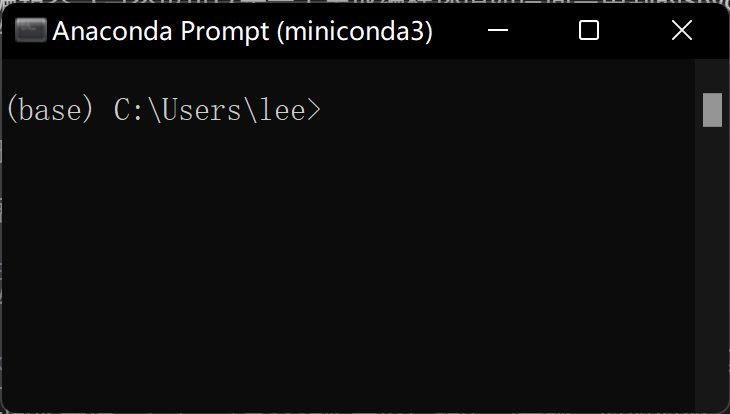
\includegraphics{images/terminal.png}

\begin{enumerate}
\def\labelenumi{\arabic{enumi}.}
\setcounter{enumi}{1}
\tightlist
\item
  Mac下,启动你的终端(Terminal),你会看到相似的界面。
\end{enumerate}

\hypertarget{ux5b89ux88c5visual-studio-code}{%
\section{安装Visual Studio Code}\label{ux5b89ux88c5visual-studio-code}}

基本上是当前最受欢迎的编程编辑器之一,可以视为记事本的替代品。

请在其\href{https://code.visualstudio.com/download}{官方网站}进行下载。

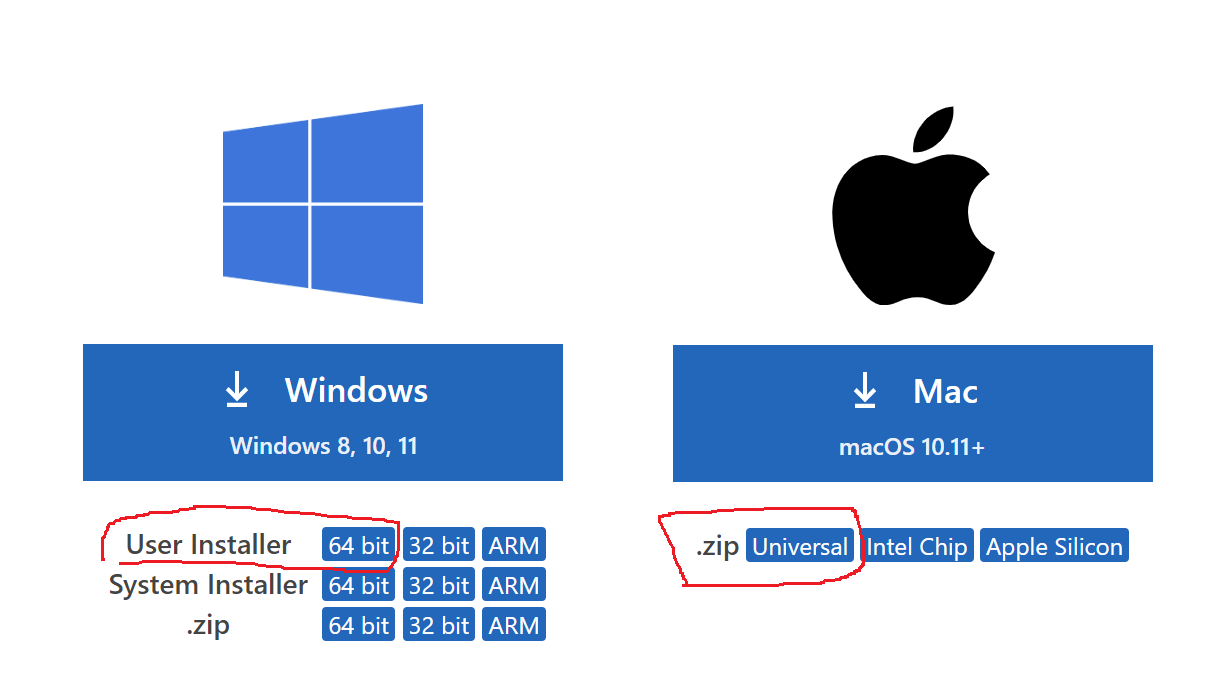
\includegraphics[width=0.9\textwidth,height=\textheight]{images/vscode_download.png}

\begin{enumerate}
\def\labelenumi{\arabic{enumi}.}
\tightlist
\item
  Windows系统请选择``User Installer 64
  bit''。安装中点选``通过Code打开\ldots''的两个选项。
  其余则一直下一步即可。
\end{enumerate}

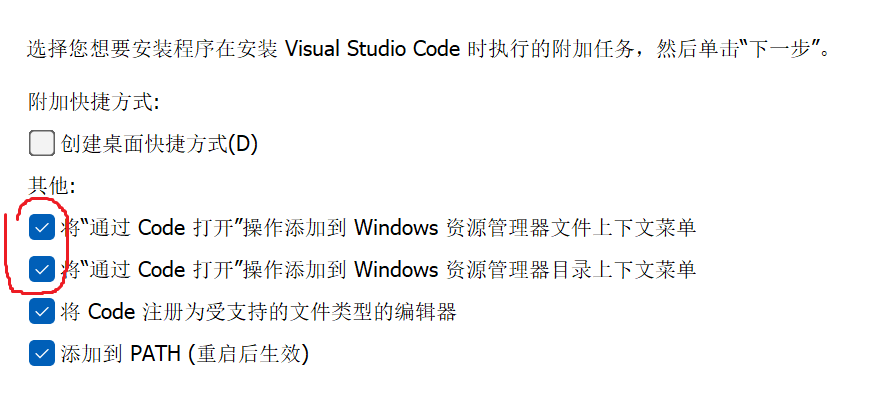
\includegraphics[width=0.9\textwidth,height=\textheight]{images/vscode_install.png}

\begin{enumerate}
\def\labelenumi{\arabic{enumi}.}
\setcounter{enumi}{1}
\tightlist
\item
  Mac系统请选择``.zip
  Universal'',下载解压后把\texttt{.app}拖到``应用程序''即可。
\end{enumerate}

\hypertarget{ux5b89ux88c5pythonux6709ux5173ux63d2ux4ef6}{%
\subsection{安装Python有关插件}\label{ux5b89ux88c5pythonux6709ux5173ux63d2ux4ef6}}

启动vscode,点击左侧工具栏的``插件按钮'',我们需要安装这几个插件:(如果是微软出品的插件,
可以看到一个蓝色底的✓标志以及Microsoft字样)。

请逐一搜索并安装,如图所示。

\begin{enumerate}
\def\labelenumi{\arabic{enumi}.}
\tightlist
\item
  \texttt{Chinese\ (Simplified)}: vscode的中文界面
\item
  \texttt{Python}: 微软出品的Python插件集合
\item
  \texttt{Jupyter}:我们后面要用到的Jupyter插件,一般已经包括在Python插件中,如果已经存在不用再安装。
\end{enumerate}


\includegraphics[width=0.6\textwidth,height=\textheight]{images/vscode_ui1.png}

至此,编程环境已经搭建完成。

\hypertarget{plusux8ba1ux7b97ux673aux7cfbux7edfux7684ux57faux672cux6982ux5ff5}{%
\chapter*{Plus:计算机系统的基本概念}\label{plusux8ba1ux7b97ux673aux7cfbux7edfux7684ux57faux672cux6982ux5ff5}}
\addcontentsline{toc}{chapter}{Plus:计算机系统的基本概念}

\markboth{Plus:计算机系统的基本概念}{Plus:计算机系统的基本概念}

\hypertarget{ux91cdux8981ux7ec4ux4ef6}{%
\section*{重要组件}\label{ux91cdux8981ux7ec4ux4ef6}}
\addcontentsline{toc}{section}{重要组件}

\markright{重要组件}

\hypertarget{ux4e00ux822cux7684ux60c5ux5f62}{%
\subsection*{一般的情形}\label{ux4e00ux822cux7684ux60c5ux5f62}}
\addcontentsline{toc}{subsection}{一般的情形}

和编程密切相关的计算机组件,不得不提的是这3件:

\begin{enumerate}
\def\labelenumi{\arabic{enumi}.}
\tightlist
\item
  中央处理器(CPU)
\item
  内存(Memory/RAM)
\item
  硬盘(Hard Drive)
\end{enumerate}

CPU:CPU的工作是进行计算,一般而言,考虑电脑运行多快,首先考虑的是CPU快不快。

内存:内存的任务是储存数据。物理上也是一块块芯片。作为储存介质,优点是速度飞快(虽然还不是最快的,CPU内部的缓存cache更快),缺点是容量相对较少,并且断电之后数据丢失。这种``快速、小容量、断电丢失数据''的储存装置,在手机的语境里可能称之为``运行内存''。

比如某些笔记本电脑,可能内存一般是8G或者16G;安卓手机比如红米K50是8G或者12G,iPhone
13是4G。老的实验室的教师机的内存是4G,学生机的内存是\ldots{} 。

硬盘:硬盘的任务也是存储数据,和内存相对,优点是容量巨大,并且断电后数据依然保留,
但速度相对内存就会慢很多很多。这种``慢速、大容量、断电保留数据''的装置,在手机语境里可能称为``闪存''。

比如有些笔记本电脑,硬盘大概512G或者1T(1024G或者1000G,看算法);典型的安卓手机比如红米K50是128G或者256G,iPhone
13有64G版、128G版等等。

显然,内存适合短时间的,反复读写的数据。硬盘适合长时间、但不用反复读写的数据保存。

如果你看到``16G + 1T''或者``8G + 256G'',可以明白指的是什么。

\hypertarget{ux624bux673aux7684ux60c5ux5f62}{%
\subsection*{手机的情形}\label{ux624bux673aux7684ux60c5ux5f62}}
\addcontentsline{toc}{subsection}{手机的情形}

手机的Soc(System on a
Chip)有些特殊,会把cpu和gpu(图形处理器)和其他一系列组件,如内存控制器,5G模块等等整合到一个芯片中。比如高通的骁龙系列,苹果的A系列,刚刚上新闻的华为的麒麟9000s,都是Soc的名称。

因此,严格来说,手机的cpu,指的是Soc里面的cpu模块,比如骁龙8
Gen2的大核Cortex-X3,小核Cortex-A720等等。

\hypertarget{ux82f9ux679cux7684mux5904ux7406ux5668}{%
\subsection*{苹果的M处理器}\label{ux82f9ux679cux7684mux5904ux7406ux5668}}
\addcontentsline{toc}{subsection}{苹果的M处理器}

特别的,最近2年苹果电脑的M系列芯片,是从苹果手机的A系列芯片发展过来,因此M1、M2等其实也是一个集成了一堆东西的Soc。

\hypertarget{ux4e2aux786cux4ef6ux5de5ux4f5cux7684ux57faux672cux6982ux5ff5}{%
\section*{3个硬件工作的基本概念}\label{ux4e2aux786cux4ef6ux5de5ux4f5cux7684ux57faux672cux6982ux5ff5}}
\addcontentsline{toc}{section}{3个硬件工作的基本概念}

\markright{3个硬件工作的基本概念}

打个比方,你要做某样工作:

\begin{enumerate}
\def\labelenumi{\arabic{enumi}.}
\tightlist
\item
  工作的时候,你就是cpu,你决定了工作的速度。
\item
  硬盘就像你的柜子,巨大能装,但拿东西不方便(比较慢)。
\item
  内存就像你的书桌,面积比较小,但你只能在上面工作。桌面的大小决定了你一次能干多少活。
\end{enumerate}

工作时候:

\begin{enumerate}
\def\labelenumi{\arabic{enumi}.}
\tightlist
\item
  你会把有关的材料,从柜子里拿到书桌上

  \begin{itemize}
  \tightlist
  \item
    CPU把数据从硬盘里读到内存中,比如Load一个游戏,打开Word写文档。
  \end{itemize}
\item
  你在书桌上开始你的工作

  \begin{itemize}
  \tightlist
  \item
    CPU开始运算,比如计算游戏角色的血量,在Word里写了一段话
  \end{itemize}
\item
  工作完毕,把工作的结果放回到柜子里

  \begin{itemize}
  \tightlist
  \item
    CPU把信息从内存保存回到硬盘中。游戏和Word文档都要存盘。
  \end{itemize}
\item
  然后清理桌面,留出空间给下一项工作。

  \begin{itemize}
  \tightlist
  \item
    CPU把有关的内存空间释放,留给其他程序
  \end{itemize}
\end{enumerate}

\hypertarget{ux673aux623fux7684ux7535ux8111}{%
\section*{机房的电脑}\label{ux673aux623fux7684ux7535ux8111}}
\addcontentsline{toc}{section}{机房的电脑}

\markright{机房的电脑}

那么,为什么机房的电脑用起来那么慢?

CPU比较旧,更重要的,内存非常小。(可能只有4G,你的手机应该也有4G起步,8G不算大。)

你的书桌或者工作台,如果面积很小会如何?

你每次只能从柜子里拿出一点材料,处理一点,然后放回柜子,然后拿出其他材料到桌子上,
然后再处理,时间都花费反复地内存和硬盘转移数据之上,并且我们也知道硬盘本身非常慢,
比内存慢一个数量级。这就导致你用一个内存(手机的运行内存)很小的电脑或者手机,会觉得特别卡。

(注意:上述描述只是一个比喻,有兴趣的同学可以自行查阅电脑的运作原理。)

\hypertarget{pythonux7a0bux5e8fux7684ux6267ux884c}{%
\chapter{Python程序的执行}\label{pythonux7a0bux5e8fux7684ux6267ux884c}}

\hypertarget{ux4e00ux4e2apythonux7a0bux5e8fux662fux4ec0ux4e48}{%
\section{一个Python程序是什么}\label{ux4e00ux4e2apythonux7a0bux5e8fux662fux4ec0ux4e48}}

写程序,就是用代码的方式,告诉计算机你要做什么。但处理器听不懂人话,因此你必须用计算机能懂的语言来做这件事。Python就是一种这样的语言。

任何一个程序都是一连串的指令,写一个程序,就是写一连串的指令。那么一个Python程序,就写一连串的Python指令。

一般情况下,我们会把这些指令保存在一个文件名的后缀(扩展名)是\texttt{.py}的文本文件里。这个文件就有点像你把一个你发明的菜谱写进一个word文档里,然后交给另一个人,他可以按你在菜谱的说明,一条条往下做,最终把菜做出来。

你在一个\texttt{.py}文件里,写出一连串的指令,然后交给Python的解释器(Interpreter)(如果你安装了Anaconda,就会有这个东西),解释器会按你在这个文件里写的指令,一条一条往下运行,最终把写的程序执行完,给你最终的结果。

我们把这个菜谱(对于Python就是\texttt{.py}文件),称之为``源代码(source
code)''。我们编程的时候,多数情况下,就是在编写(或者一边写一边运行)这个\texttt{.py}文件(数据分析的时候常用notebook格式的文件,后面会讲到)。

这个文件本质上一个\texttt{.txt}文件没什么不同,都可以用任何文本编辑器(例如你电脑里的``记事本'',以及我们前面安装的vscode)打开和编辑。

因此,所谓的编程就是:

\begin{enumerate}
\def\labelenumi{\arabic{enumi}.}
\tightlist
\item
  用一个文本编辑器,如我们后面用的vscode(或者一个集成编程环境如PyCharm),编辑一个\texttt{.py}文件
\item
  把你要的代码写进去。
\item
  用不同的方法去执行这个文件里代码。可能是在系统里一次性执行整个文件里所有代码,也可能是在一个交互环境里一步一步地执行。
\item
  循环2和3,直到得到你满意的结果。
\end{enumerate}

\hypertarget{ext_name}{%
\subsection{预备知识:扩展名和文件类型}\label{ext_name}}

用于表示某个文件是什么类型,一般我们会看文件名的最后一个英文\texttt{.}以及之后的内容。

\textbf{注意}:这里只是讨论一般的情况。扩展名也是可以修改的,所以未必和实际的文件类型一致。

\begin{enumerate}
\def\labelenumi{\arabic{enumi}.}
\tightlist
\item
  一个文件,其名为\texttt{WINWORD.EXE},其扩展名为\texttt{.exe}(Windows系统和Mac系统的文件名不区分大小写,但一般建议还是考虑大小写问题),则意味着这是一个``Windows系统的可执行文件''。这实际上是微软Windows版本office中的Word的主程序。我们(在windows下)常说的``运行一个程序'',就是执行一个exe文件。
\item
  一个文件,其名为\texttt{鲁迅全集.txt},其扩展名为\texttt{.txt},则意味着这是一个``纯文本文件'',其中的所有内容都可以视为文字,可以用任何一个文本编辑器,例如记事本,或者Word打开。
\item
  其他扩展名,如\texttt{.jpg}是常见的图形文件,\texttt{.docx}是2007版本以后的Word文档,等等等等。
\end{enumerate}

\hypertarget{ux91cdux8981windowsux4e0bux6b63ux786eux663eux793aux6587ux4ef6ux7684ux6269ux5c55ux540d}{%
\subsection{(重要)Windows下正确显示文件的扩展名}\label{ux91cdux8981windowsux4e0bux6b63ux786eux663eux793aux6587ux4ef6ux7684ux6269ux5c55ux540d}}

默认情况下,windows系统会因此已知文件类型的扩展名,我们要把文件完整地显示出来,需要修改一个设置。

在开始菜单,搜索``文件资源管理器选项'' -\textgreater{} ``查看''页面
-\textgreater{} 去掉``隐藏已知文件类型的扩展名''前面的勾选。

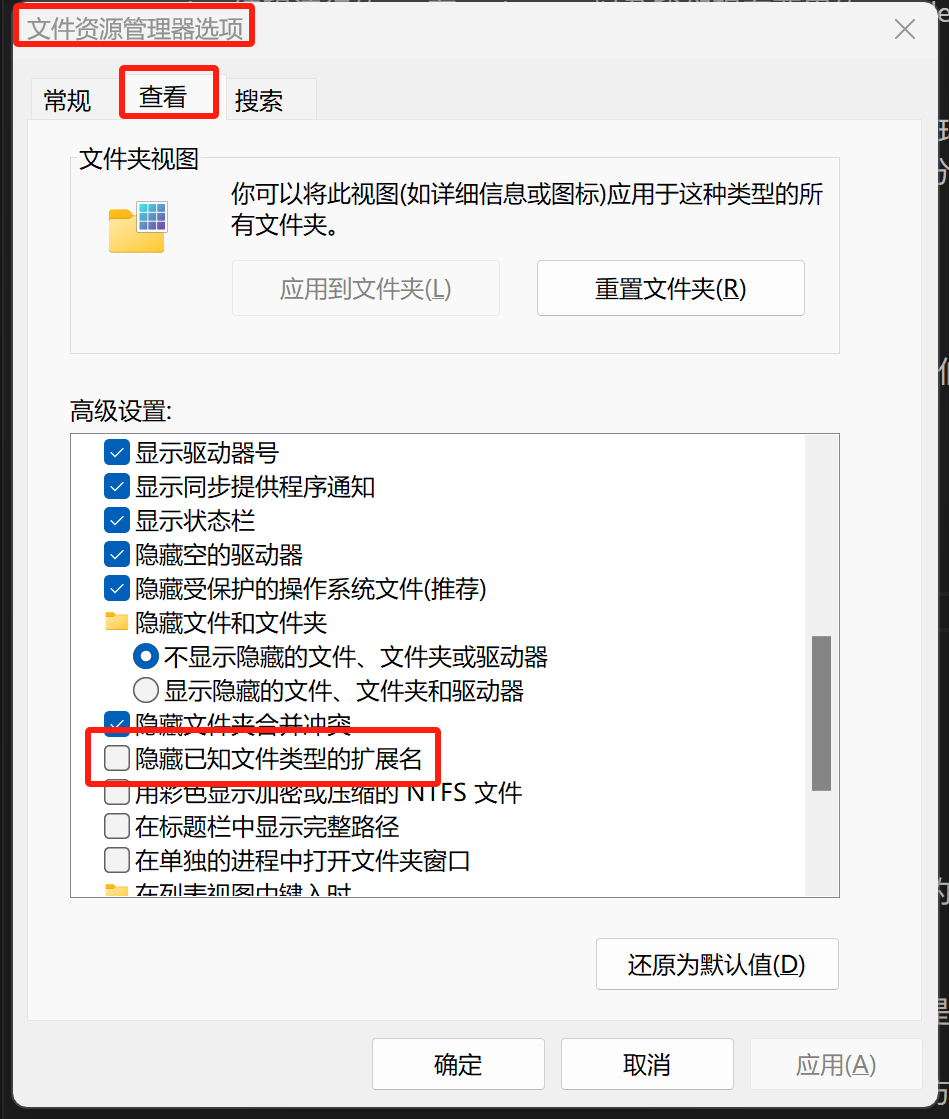
\includegraphics[width=0.8\textwidth,height=\textheight]{images/显示扩展名.png}

这样,在你的资源管理器中,显示文件的时候就会显示文件全名。

\hypertarget{python_interactive}{%
\section{Python的交互式环境}\label{python_interactive}}

我们先采用最基本的Python的交互式环境,给大家一点运行程序的感觉。

\begin{enumerate}
\def\labelenumi{\arabic{enumi}.}
\tightlist
\item
  启动Anaconda Prompt。(用Mac的同学,启动终端terminal)
\end{enumerate}


\includegraphics{images/Anaconda_icon.png}

\begin{enumerate}
\def\labelenumi{\arabic{enumi}.}
\setcounter{enumi}{1}
\tightlist
\item
  我们会看到命令行窗口
\end{enumerate}

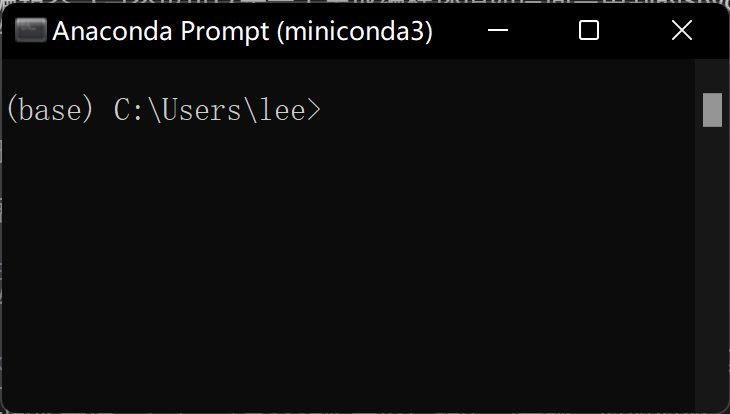
\includegraphics{images/terminal.png}

\begin{enumerate}
\def\labelenumi{\arabic{enumi}.}
\setcounter{enumi}{2}
\tightlist
\item
  输入\texttt{python\ \textless{}回车\textgreater{}},我们可以进入python的交互式运行环境。
\end{enumerate}

这个命令会启动我们所说的Python的解释器:你在其中输入Python语句,会被解释器翻译成电脑听得到的机器代码。

{\textbf{注意:}}
其中的命令提示符\texttt{\textgreater{}\textgreater{}\textgreater{}}。三个右侧尖括号,表示\textbf{我们正处于python的交互式环境中},此时我们可以执行python的语句。

同时可见截图中的Python的版本为3.9.5,你安装的版本应该会更高。

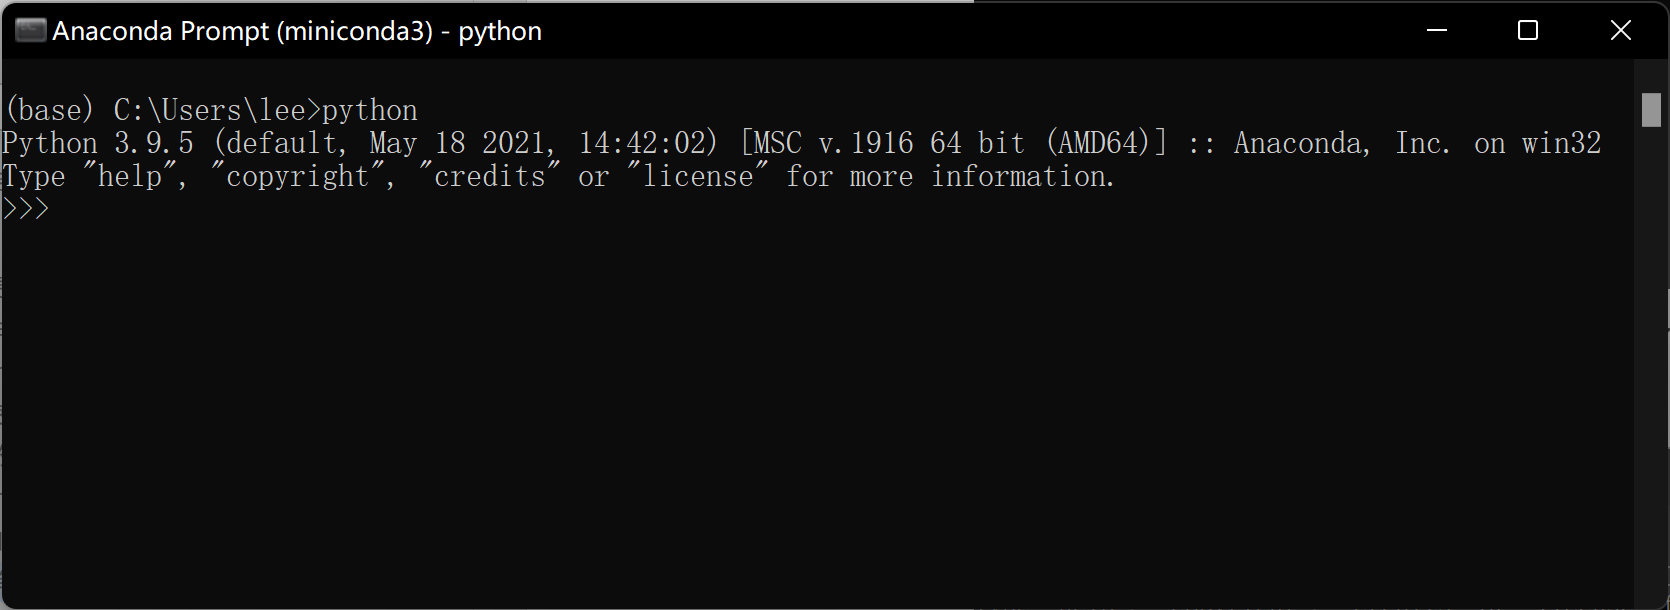
\includegraphics{images/python-interactive.png}

\hypertarget{ux7b80ux5355ux7684ux7f16ux7a0bux8ba1ux7b971-2}{%
\subsection{简单的编程:计算1 +
2}\label{ux7b80ux5355ux7684ux7f16ux7a0bux8ba1ux7b971-2}}

\begin{enumerate}
\def\labelenumi{\arabic{enumi}.}
\tightlist
\item
  我们依次输入(每行代码以结束)
\end{enumerate}

\begin{Shaded}
\begin{Highlighting}[]
\OperatorTok{\textgreater{}\textgreater{}\textgreater{}}\NormalTok{ a }\OperatorTok{=} \DecValTok{1}
\OperatorTok{\textgreater{}\textgreater{}\textgreater{}}\NormalTok{ b }\OperatorTok{=} \DecValTok{2}
\OperatorTok{\textgreater{}\textgreater{}\textgreater{}}\NormalTok{ c }\OperatorTok{=}\NormalTok{ a }\OperatorTok{+}\NormalTok{ b }
\OperatorTok{\textgreater{}\textgreater{}\textgreater{}} \BuiltInTok{print}\NormalTok{(c)}
\end{Highlighting}
\end{Shaded}

显然,1+2必然得到

\begin{Shaded}
\begin{Highlighting}[]
\DecValTok{3}
\end{Highlighting}
\end{Shaded}

\begin{enumerate}
\def\labelenumi{\arabic{enumi}.}
\setcounter{enumi}{1}
\tightlist
\item
  结果大致如图
\end{enumerate}

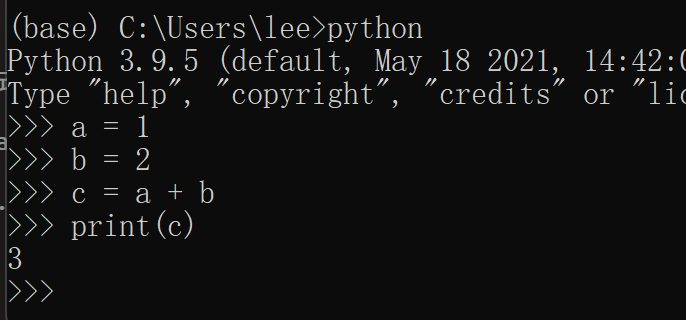
\includegraphics{images/basic_add.png}

{\textbf{注意:}}

\begin{itemize}
\tightlist
\item
  无法得到结果\texttt{3},首先检查有没有\textbf{输入错误(打错字)}。
\item
  \texttt{print(c)}中的小括号,是英文括号。在语法层面上的所有符号,都是\textbf{英文符号}。
\item
  如果输入的代码有误,已经敲了回车,只要把正确代码的再输入一次即可。
\end{itemize}

\hypertarget{ux4e0aux8ff0ux7a0bux5e8fux4e2dux6d89ux53caux7684ux4e00ux4e9bux6982ux5ff5}{%
\subsection{上述程序中涉及的一些概念}\label{ux4e0aux8ff0ux7a0bux5e8fux4e2dux6d89ux53caux7684ux4e00ux4e9bux6982ux5ff5}}

这个涉及程序设计的几个基本概念:

\begin{enumerate}
\def\labelenumi{\arabic{enumi}.}
\tightlist
\item
  变量和赋值
\end{enumerate}

变量,顾名思义,一个可变的量。编程中变量的概念和代数中的\texttt{x},
\texttt{y}, \texttt{z}基本一样。 Python中,对变量赋值使用1个等号
``\texttt{=}''。 显然, 我们有3个变量,\texttt{a},
\texttt{b}和\texttt{c}。我们把\texttt{1}赋予\texttt{a},\texttt{2}赋予\texttt{b},把\texttt{a\ +\ b}的值赋予\texttt{c}。

\begin{enumerate}
\def\labelenumi{\arabic{enumi}.}
\setcounter{enumi}{1}
\tightlist
\item
  运算符
\end{enumerate}

加减乘除,以及逻辑运算如是否等于,大于,小于等,我们以后会用到。这里只用到``加法''

\begin{enumerate}
\def\labelenumi{\arabic{enumi}.}
\setcounter{enumi}{2}
\tightlist
\item
  函数
\end{enumerate}

和数学函数一样,我们调用一个函数,给这个函数传递一个参数,然后这个函数会根据这个参数做一些事情。可能是为你进行一个计算,可能修改某个变量等等,也可能什么都不做。

这里我们调用的函数是\texttt{print()},这个函数的用途是把你传递给他的变量\texttt{c}的值打印出来。函数的调用方法是函数名与小括号。

\textbf{数据分析的程序,大部分情况下可以视为由变量和函数组成。}

\hypertarget{ux9000ux51faux8fd0ux884cux73afux5883}{%
\subsection{退出运行环境}\label{ux9000ux51faux8fd0ux884cux73afux5883}}

输入\texttt{exit()},然后回车即可。

可见,\texttt{exit}本身也是一个函数(函数名+小括号),其调用这个函数的作用是退出Python交互式运行环境。

{\textbf{注意:}}一定要退出,以便后续的程序能执行。

此时,我们又回到了一开始的命令行(终端)环境中

可见,命令提示符现在是一个\texttt{\textgreater{}},这提示我们正处于系统的命令行环境中

\begin{enumerate}
\def\labelenumi{\arabic{enumi}.}
\tightlist
\item
  可以执行系统中的命令,但不能执行python中的语句!
\item
  要进行交互式的python编程,要首先进入\protect\hyperlink{python_interactive}{Python的交互式环境}中!
\end{enumerate}

\hypertarget{ux8865ux5145ux8defux5f84}{%
\section{补充:路径}\label{ux8865ux5145ux8defux5f84}}

\hypertarget{path}{%
\subsection{路径Path}\label{path}}

\emph{你的文件或者文件夹(目录),到底保存到了哪里?}

所谓路径(path),到达某个文件或者文件夹(目录)的层级结构,每一层用一个斜杠``\texttt{/}''分割。

在命令行(终端)环境下,在命令提示符\texttt{\textgreater{}}之前,一般会有提示你当前路径,即当前你处于哪个目录下。

例如
\texttt{C:\textbackslash{}Users\textbackslash{}lee},指的就是,在你的\texttt{C}盘下,\texttt{Users}目录下,的\texttt{lee}目录。

{\textbf{注意}}
{\textbf{注意:}}在你的电脑上,这里的\texttt{lee}会替换为你的用户名

这样,你输入的任何命令,都会对``当前路径''生效。

同样,路径既可以指向一个目录(文件夹),也可以指向一个文件。

如\texttt{C:\textbackslash{}Users\textbackslash{}lee\textbackslash{}add.py},就指的是,在你的\texttt{C}盘下的\texttt{Users}目录下的\texttt{lee}目录下的一个叫\texttt{add.py}的文件。

\hypertarget{ux76f8ux5bf9ux8defux5f84ux548cux7eddux5bf9ux8defux5f84}{%
\subsection{相对路径和绝对路径}\label{ux76f8ux5bf9ux8defux5f84ux548cux7eddux5bf9ux8defux5f84}}

\begin{enumerate}
\def\labelenumi{\arabic{enumi}.}
\tightlist
\item
  绝对路径:从根目录(windows下即一个盘符,如c盘或者d盘)开始的路径,可以确定无疑地指向某个文件或者目录。如\texttt{C:\textbackslash{}Users\textbackslash{}lee\textbackslash{}add.py}。
\item
  相对路径:不从根目录起始的路径。其指向的目的地,从你的``当前路径''开始,往下数。
\end{enumerate}

假如,你的当前路径是\texttt{C:\textbackslash{}Users},那么此时,相对路径\texttt{lee\textbackslash{}add.py},所指向的,就是当前路径下(\texttt{C:\textbackslash{}Users}),\texttt{lee}目录下的\texttt{add.py}。这也等价于绝对路径\texttt{C:\textbackslash{}Users\textbackslash{}lee\textbackslash{}add.py}。

\begin{enumerate}
\def\labelenumi{\arabic{enumi}.}
\setcounter{enumi}{2}
\tightlist
\item
  两者的区别:绝对路径从根目录开始,相对路径从``当前路径''开始。
\end{enumerate}

\hypertarget{ux8fdbux5165ux67d0ux4e2aux76eeux5f55}{%
\subsection{进入某个目录}\label{ux8fdbux5165ux67d0ux4e2aux76eeux5f55}}

Windows命令行,和Mac的终端,有相同的命令\texttt{cd\ \textless{}路径\textgreater{}},可以进入一个目录。

如,在终端中输入(并回车)注意这里使用的是绝对路径

\begin{verbatim}
cd C:/Users 
\end{verbatim}

则会让终端进入到 \texttt{C:/Users}
目录下。见提示符\texttt{\textgreater{}}前方的``当前路径''已经改变为\texttt{C:/Users}。你现在已经位于\texttt{C:/Users}
目录。

尝试相对路径,在终端中输入(并回车),注意这里的\texttt{lee},请替换成你的用户名。

\begin{verbatim}
cd lee
\end{verbatim}

则会让终端进入到 \texttt{C:/Users/lee}
目录下。见提示符\texttt{\textgreater{}}前方的``当前路径''已经改变为\texttt{C:/Users/lee}。你现在已经位于\texttt{C:/Users/lee}
目录。

其他用法包括:

\begin{enumerate}
\def\labelenumi{\arabic{enumi}.}
\tightlist
\item
  进入上一级目录
\end{enumerate}

\begin{verbatim}
cd ..
\end{verbatim}

\begin{enumerate}
\def\labelenumi{\arabic{enumi}.}
\setcounter{enumi}{1}
\tightlist
\item
  进入根目录
\end{enumerate}

\begin{verbatim}
cd /
\end{verbatim}

可以让你在命令行和终端中,定位到你想要的目录和文件。

\hypertarget{use_win}{%
\subsection{用Windows图形界面获得路径}\label{use_win}}

在你的windows资源管理器(俗称``我的电脑''),在任何一个文件夹中,点击地址栏

你就可以得到这个文件夹的路径,可以粘贴到命令行中。

{\textbf{特别注意:正反斜杠问题}}

在编程的语境下,反斜杠``\texttt{\textbackslash{}}''有特殊用途。因此,表示路径的时候,我们统一用(正)斜杠``\texttt{/}'',而不用反斜杠``\texttt{\textbackslash{}}''。

统一的写法,如\texttt{C:/Users/lee}

\hypertarget{ux5217ux76eeux5f55}{%
\subsection{列目录}\label{ux5217ux76eeux5f55}}

列目录的命令,Windows的命令行中为\texttt{dir},Mac中为\texttt{ls}。同学们可以执行尝试。

\hypertarget{ux4f7fux7528visual-studio-code}{%
\chapter{使用Visual Studio Code}\label{ux4f7fux7528visual-studio-code}}

我们一般不会直接在命令行界面进行编程, 而会利用一个集成编程环境(IDE),
为我们提供文件管理、语法提示、自动补全等等功能。
Python编程流行的IDE有PyCharm,以及我们现在要用的vscode文字编辑器+Python相关插件。

这些集成编辑环境,通常会把.py文件的编辑和python的交互环境结合起来,让我们一边编辑py文件的同时,一边执行代码并查看结果。数据分析完毕时,代码同时也写成了。

\hypertarget{ux4ee3ux7801ux7684ux5b58ux653e}{%
\section{代码的存放}\label{ux4ee3ux7801ux7684ux5b58ux653e}}

在正式开始之前,选择一个存放代码等等有关文件的文件夹。
为了便于演示,这里选择在桌面上新建一个``python\_class''的文件夹,
作为本课程有关代码的存放地点。

但一般建议选择一个比较好的目录,比如你可能有一个地方是专门用来存放课程的地方(比如在``我的文档''下),
在此位置建立python\_class较好。这里选择桌面仅仅是为了方便演示。

注:课程文件夹不要放在在C盘根目录下,可能有权限问题。

打开vscode,文件,打开文件夹,打开vscode中的资源管理器,我们发现什么都没有。

\hypertarget{ux5efaux7acbux7684ux4e00ux4e2aux6e90ux4ee3ux7801ux6587ux4ef6}{%
\section{建立的一个源代码文件}\label{ux5efaux7acbux7684ux4e00ux4e2aux6e90ux4ee3ux7801ux6587ux4ef6}}

选择文件,新建文本文件,直接保存,给这个空白文件起一个名字,如``001.py''。
注意,扩展名必须是``.py''。

当你在vscode编译一个py文件,vscode会自动调用所以和python有关的插件。
vscode会从一个文本编辑器,成为一个集编辑、运行、调试于一身的Python集成开发环境。

当然,你用vscode来写其他语言的代码也可以。

\hypertarget{vscodeux7684ux754cux9762}{%
\section{vscode的界面}\label{vscodeux7684ux754cux9762}}

右上角出现了播放按钮▶,可以把当前文件的代码从头到尾执行一次。

右下角出现了Python字样,现在进入了Python代码编辑模式。

如果出现了黄底色的Select Interpreter字样,是没指定解释器。等于再问,
写好的代码交给谁来执行?

点一下,在弹出的框中选择conda。

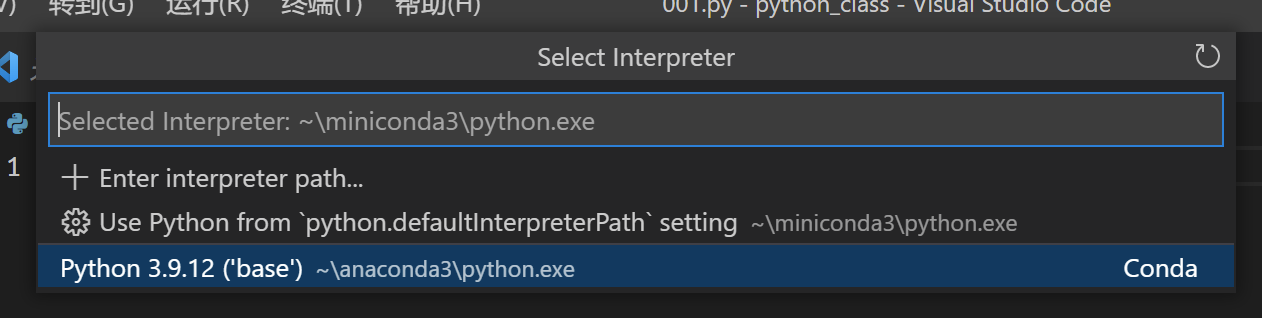
\includegraphics{images/select_interpreter.png}

\hypertarget{ux7b2cux4e00ux6bb5ux4ee3ux7801}{%
\section{第一段代码}\label{ux7b2cux4e00ux6bb5ux4ee3ux7801}}

我们在文件里写如如下代码,保存(ctrl+s)。

就算你完全不懂python,凭感觉也可以知道这段代码是打印两个变量相加的结果。

\begin{Shaded}
\begin{Highlighting}[]
\NormalTok{a }\OperatorTok{=} \DecValTok{1}
\NormalTok{b }\OperatorTok{=} \DecValTok{2}
\NormalTok{c }\OperatorTok{=}\NormalTok{ a }\OperatorTok{+}\NormalTok{ b}
\BuiltInTok{print}\NormalTok{(c)}
\end{Highlighting}
\end{Shaded}

\hypertarget{ux9884ux5907ux77e5ux8bc6pythonux7684ux6ce8ux91cacomment}{%
\subsection{预备知识:Python的注释(comment)}\label{ux9884ux5907ux77e5ux8bc6pythonux7684ux6ce8ux91cacomment}}

先说注释。Python使用井号:\texttt{\#}来表示注释。所谓注释,就是``\textbf{给人看}''的内容,而Python的解释器会直接忽略掉这部分。

\begin{enumerate}
\def\labelenumi{\arabic{enumi}.}
\tightlist
\item
  注释可以出现在任何地方,注意\texttt{\#}号只会影响同一行右边的代码,因此也可以出现在行尾。
\item
  注释往往也可以用来临时屏蔽一部分代码,只要在代码的最左侧插入一个\texttt{\#},那么整行代码会被Python解释器忽略。这是常用技巧。
\end{enumerate}

我们尝试写几个注释,例如:

\begin{Shaded}
\begin{Highlighting}[]
\CommentTok{\# 这段代码会计算a和b相加的结果}
\NormalTok{a }\OperatorTok{=} \DecValTok{1}
\NormalTok{b }\OperatorTok{=} \DecValTok{2}
\NormalTok{c }\OperatorTok{=}\NormalTok{ a }\OperatorTok{+}\NormalTok{ b }\CommentTok{\# 这行代码会计算 a + b}

\CommentTok{\# 下面的代码会把c的值打印出来}
\BuiltInTok{print}\NormalTok{(c)}
\end{Highlighting}
\end{Shaded}

注释是对代码的说明,非常重要:

\begin{enumerate}
\def\labelenumi{\arabic{enumi}.}
\tightlist
\item
  写代码时间长了,肯定会不记得自己写的内容。有时候上午写的,下午就会忘记。
\item
  多人合作的时候,要读懂彼此的代码,也必须有良好的注释。
\end{enumerate}

特别地,\textbf{注释是考试的给分点}。你的考试程序输出了正确的结果,可以得到合格评价,同时具有良好的编写风格、合理的注释,才能得到更高分。

\hypertarget{ux6267ux884c}{%
\section{执行}\label{ux6267ux884c}}

代码写好了,执行有几种方式。

\hypertarget{run-python-file-ux6309ux94ae}{%
\subsection{Run Python File 按钮 ▶}\label{run-python-file-ux6309ux94ae}}

点击右上角的播放按钮Run Python
File,会把当前的py文件,从头到尾执行一次。
你会看到输出了结果\texttt{3}。

点击垃圾桶图标🗑,终止这个终端。

一般而言,要把文件从头到尾执行一次,就可以用这种方式。

\hypertarget{ux4e92ux52a8ux6267ux884c}{%
\subsection{互动执行}\label{ux4e92ux52a8ux6267ux884c}}

如果你要做数据分析之类的任务,需要一般看结果一边写代码,我们会选择互动执行的方式。

使用一种特殊的注释\texttt{\#\ \%\%}(井号,2个百分号,中间可以有空格),一般称为``cell
separator'' 可以把python代码分成一个一个的cell。试一下:

\begin{Shaded}
\begin{Highlighting}[]
\CommentTok{\# \%\%}
\NormalTok{a }\OperatorTok{=} \DecValTok{1}
\NormalTok{b }\OperatorTok{=} \DecValTok{2}
\BuiltInTok{print}\NormalTok{(a)}
\BuiltInTok{print}\NormalTok{(b)}

\CommentTok{\# \%\%}
\NormalTok{c }\OperatorTok{=}\NormalTok{ a }\OperatorTok{+}\NormalTok{ b}
\BuiltInTok{print}\NormalTok{(c)}
\end{Highlighting}
\end{Shaded}

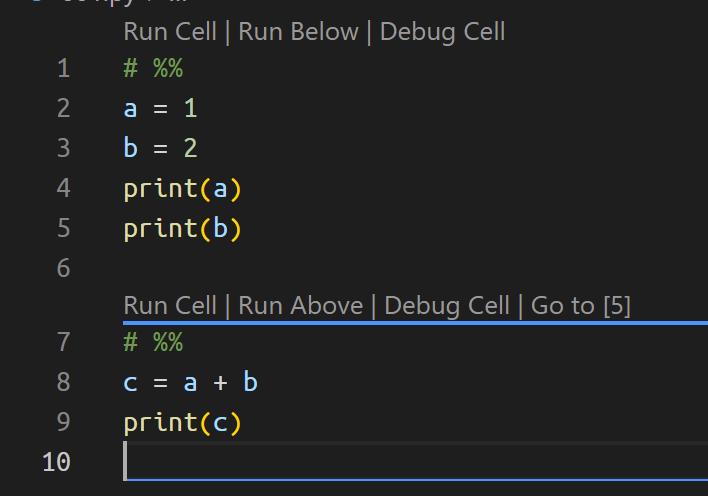
\includegraphics{images/runcell.png}

\texttt{\#\ \%\%} cell
seperator把代码切成了一块一块:两行seperator中间的部分,被视为一个cell。

我们点击第一个run cell,终端只会执行第一个cell,即1到6行的代码。

这一块代码会打印出变量\texttt{a}和\texttt{b}的值。

点开终端上的省略号,可以看到这个cell具体执行了什么代码。

同理,点击第二个run cell会执行下一块代码,计算a+b并打印c。

但一般我们用快捷键:

Ctrl + 回车:执行当前cell。(Mac系统可能是Cmd + 回车) Shift +
回车:执行当前cell,并跳到下一个cell。

所以,你可以按住Shift,连续按回车,就可以一个cell一个cell往下执行。

这在进行数据分析的时候会用很多。

单步执行和debug会在后面专门说。

特别地,在互动执行下,每个cell的最后一行的结果会自动显示。
如果只是查看变量的值,这可以让我们少打一个\texttt{print()}或者\texttt{display()}。
注意这只在互动模式下生效。

尝试:把上述代码的\texttt{print(a)}和\texttt{print(b)}改写。

\hypertarget{ux53d8ux91cfux8868}{%
\subsection{变量表}\label{ux53d8ux91cfux8868}}

在交互执行的过程中,点击变量表,可以查看当前运行环境中的变量的信息。

\hypertarget{ux8131ux79bbvscodeux6267ux884c}{%
\subsection{脱离vscode执行}\label{ux8131ux79bbvscodeux6267ux884c}}

python本身是一个独立的可执行程序,和vscode并无关系。这个可执行程序即所谓解释器,
会把源代码从第一行到最后以后执行一次。

因此,你只要告诉python你要执行哪个.py文件即可。

这个一般教程会放在第一部分,但以我们的任务更多是要交互执行,这里只简单演示一下。

在你anaconda prompt或者终端中,进入你刚才新建的python\_class目录。

\begin{Shaded}
\begin{Highlighting}[]
\NormalTok{python }\FloatTok{001.}\ErrorTok{py}
\end{Highlighting}
\end{Shaded}

结果是一样的。

实际上,右上角的播放按钮,做的是同样的事,只是把多个步骤(进入anaconda环境,
进入工作目录,输入python 001.py等)合并成一个按钮。

\hypertarget{vscodeux4e2dux4ee3ux7801ux51faux9519}{%
\section{vscode中代码出错}\label{vscodeux4e2dux4ee3ux7801ux51faux9519}}

\hypertarget{ux8fd0ux884cux5355ux5143ux683crun-cellux51faux73b0-bad-file-descriptor-ux9519ux8bef}{%
\subsection{运行单元格(run cell)出现 Bad file descriptor
错误}\label{ux8fd0ux884cux5355ux5143ux683crun-cellux51faux73b0-bad-file-descriptor-ux9519ux8bef}}

如果你用的是Windows,且你的用户名是中文,那么用vs code的run
cell运行,可能会出现如下错误:

(这是某位同学的笔记本电脑,请大家要经常清理自己电脑的屏幕)


\includegraphics{images/vscode_run_cell_error.jpg}

注意最后一行

\begin{verbatim}
Bad file descriptor (bundled\zeromq\src\epoll.cpp:100)
\end{verbatim}

这个问题可能是中文用户名有关,某个组件(pyzmq)新版本处理中文路径会出错。处理方法有2种,
第一种已经在部分同学的电脑上验证过了,第二钟则尚未验证。

\textbf{方法1:改环境变量}

在windows菜单中选择''编辑系统环境变量''


\includegraphics[width=0.6\textwidth,height=\textheight]{images/edit_var_menu.png}

在弹出的窗口中选择最下方的``环境变量(N)''

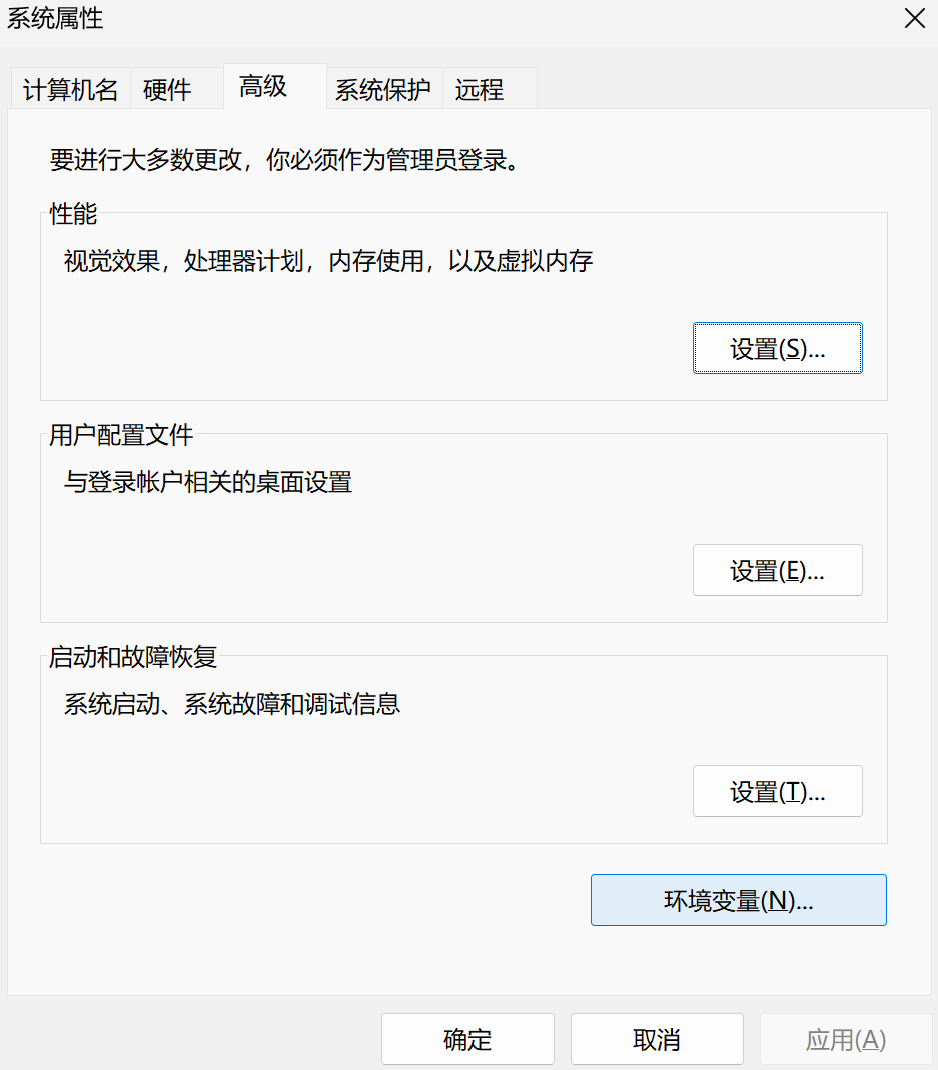
\includegraphics[width=0.6\textwidth,height=\textheight]{images/edit_var_panel.png}

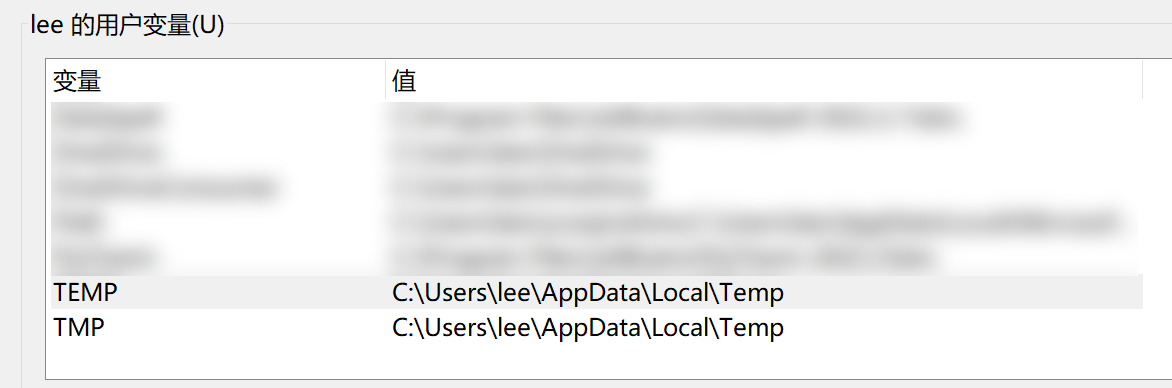
\includegraphics[width=0.6\textwidth,height=\textheight]{images/env_vars_01.png}

可见最下方有\texttt{TEMP}和\texttt{TMP}2个环境变量(临时文件所在目录)。双击2个环境变量,都改为\texttt{C:\textbackslash{}Temp}。

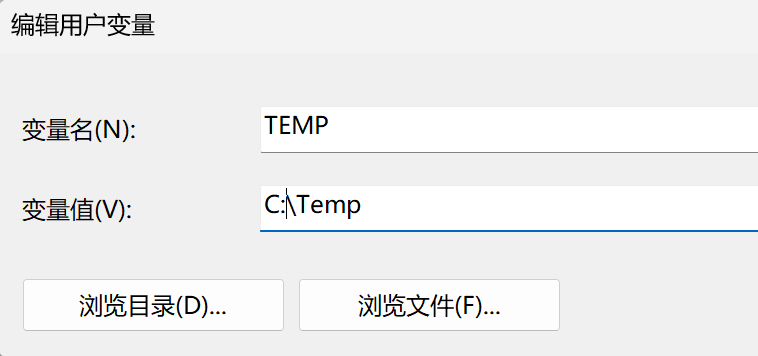
\includegraphics[width=0.6\textwidth,height=\textheight]{images/tmp_var.png}

最终如图。

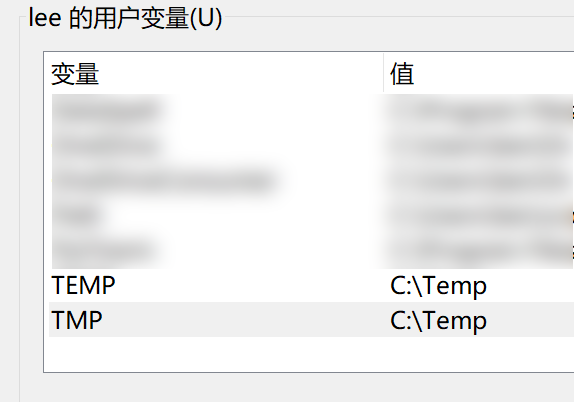
\includegraphics[width=0.6\textwidth,height=\textheight]{images/tm_var_after.png}

重启电脑即可。

\textbf{方法2:降级pyzmq}

进入anaconda prompt(见前一章),依次执行代码

\begin{verbatim}
pip uninstall pyzmq <回车>
pip install pyzmq==19.0.2 <回车>
\end{verbatim}

重启vs code即可。

\hypertarget{ux627eux4e0dux5230anaconda}{%
\subsection{找不到Anaconda}\label{ux627eux4e0dux5230anaconda}}

如果不在默认的路径上安装anaconda,比如转移到了d盘,可能在选择解释器(select
interpreter)的时候,找不到正确的conda和python路径。这时候需要手动设置你的conda安装路径。

在vscode界面的左下角点击``管理(齿轮图标)'' -\textgreater{}
``设置'',搜索'conda',一般有三个选项:

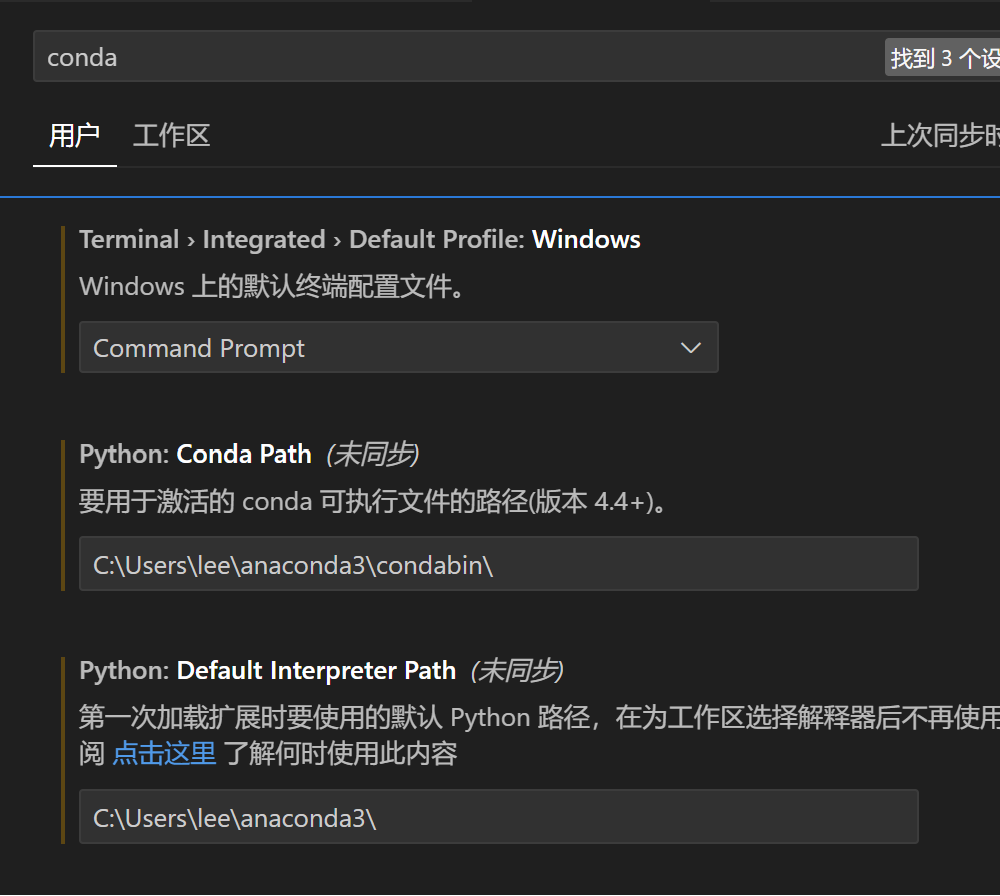
\includegraphics[width=0.8\textwidth,height=\textheight]{images/conda_path.png}

\begin{enumerate}
\def\labelenumi{\arabic{enumi}.}
\tightlist
\item
  \texttt{Conda\ Path}选择你安装conda路径加上\texttt{\textbackslash{}condabin\textbackslash{}}。例如你装到了\texttt{D:\textbackslash{}anaconda3\textbackslash{}}下,那么路径就是\texttt{D:\textbackslash{}anaconda3\textbackslash{}condabin\textbackslash{}}。
\item
  \texttt{Default\ Interpreter\ Path}选择你安装anaconda的路径,按上面的例子,就是\texttt{D:\textbackslash{}anaconda3\textbackslash{}}
\end{enumerate}

这时候再进行前面选择解释器的过程,应该就找到conda和解释器了。

\hypertarget{ux6267ux884cux6574ux4e2aux6587ux4ef6ux53efux4ee5ux5f97ux5230ux6b63ux786eux7ed3ux679cux4f46ux8fd8ux662fux6709ux4e00ux4e32ux7ea2ux5b57}{%
\subsection{执行整个文件,可以得到正确结果,但还是有一串红字}\label{ux6267ux884cux6574ux4e2aux6587ux4ef6ux53efux4ee5ux5f97ux5230ux6b63ux786eux7ed3ux679cux4f46ux8fd8ux662fux6709ux4e00ux4e32ux7ea2ux5b57}}

比如你``执行整个文件(右上角的播放按钮)'',最后可以得到结果(比如``3''),但是首次执行的时候出现一串红字错误,然后才是正确结果(这里一时找不到截图),那么可以用上面的方法,把截图中的第一个选项Terminal,设定为\texttt{Command\ Prompt},和截图保持一致即可。

\hypertarget{ux53d8ux91cfux548cux5e38ux7528ux7c7bux578b}{%
\chapter{变量和常用类型}\label{ux53d8ux91cfux548cux5e38ux7528ux7c7bux578b}}

本章节介绍Python中的变量和基础类型,完成本章之后,可以把Python当成计算器和草稿纸。本章没有要提交的课堂作业。

从这章起就要开始编程,有一件事要预先强调:\textbf{所有语句中的符号都是英文},比如冒号,引号等等,达成中文符号是错误的一大来源。但vscode可能会提示你,后面大家会知道。

\hypertarget{ux53d8ux91cf}{%
\section{变量}\label{ux53d8ux91cf}}

前面说过,Python(或者其他编程语言)中的变量,和你数学课上的\texttt{x,\ y,\ z}是同类的概念。

正如前面的例子,Python使用等号\texttt{=}来为一个变量赋值

\begin{Shaded}
\begin{Highlighting}[]
\CommentTok{\#\%\% 赋值与重新赋值}
\NormalTok{a }\OperatorTok{=} \DecValTok{1}
\NormalTok{a }\OperatorTok{=} \DecValTok{2}
\BuiltInTok{print}\NormalTok{(a)}
\end{Highlighting}
\end{Shaded}

\begin{verbatim}
2
\end{verbatim}

假如这个变量\texttt{a}一开始不存在,那么赋值的同时,也会把这个变量创造出来。

对于Python语言,这个过程(\textbf{不严格地说})大致是:

\begin{enumerate}
\def\labelenumi{\arabic{enumi}.}
\tightlist
\item
  (绑定)Python在电脑的内存空间找了一个空地,创建了一个对象(object),存放了\texttt{1}这个值,然后把\texttt{a}这个名字,和这个对象绑定起来。
\item
  (重绑定)当我们对变量\texttt{a}赋其他值的时候,如\texttt{a\ =\ 2}的时候,Python另外创建了一个对象,存放了\texttt{2}这个值,然后把\texttt{a}这个名字,重新绑定到这个新的对象上。
\item
  (引用)变量名,就像一个内存中的对象的标签。引用这个名字,就是引用其表示的对象。
\end{enumerate}

\hypertarget{ux5220ux9664ux4e00ux4e2aux53d8ux91cf}{%
\subsection{删除一个变量}\label{ux5220ux9664ux4e00ux4e2aux53d8ux91cf}}

使用del语句

\begin{Shaded}
\begin{Highlighting}[]
\CommentTok{\#\%\% 删除变量}
\NormalTok{a }\OperatorTok{=} \DecValTok{1}
\KeywordTok{del}\NormalTok{ a}
\BuiltInTok{print}\NormalTok{(a)}
\end{Highlighting}
\end{Shaded}

因为变量\texttt{a}已经被我们删除了,所以你再次引用\texttt{a}的时候,Python会告诉你,

\begin{verbatim}
NameError: name 'a' is not defined
\end{verbatim}

\hypertarget{ux5e38ux89c1ux9519ux8befname-not-defined}{%
\subsection{常见错误name not
defined}\label{ux5e38ux89c1ux9519ux8befname-not-defined}}

\begin{verbatim}
NameError: name 'xxx' is not defined
\end{verbatim}

这个错误要告诉你,xxx这个东西,python找不到。这可能是:

\begin{enumerate}
\def\labelenumi{\arabic{enumi}.}
\tightlist
\item
  打错字。例如你要引用一个名字叫\texttt{apple},但输入成了\texttt{appla}。vscode会有提示。
\item
  代码存放在其他地方,没有import,后面会讲。
\item
  引用了一个不存在的变量。
\end{enumerate}

稍微解释下第3点:

\begin{enumerate}
\def\labelenumi{\arabic{enumi}.}
\tightlist
\item
  一个重新启动的Python交互环境,可以理解为一片白纸(其实不是完全是)。
\item
  第一次执行\texttt{a\ =\ 1}语句之后,\texttt{a}这个变量才会存在。
\item
  \texttt{.py}文件中,有\texttt{a=1}这个语句,如果你不\textbf{执行一次},内存中也不会有\texttt{a}。
\end{enumerate}

这表示,你只是\textbf{打开一个.py文件},其实交互环境里面还是什么都没有,
这个时候\texttt{print(a)},就会提示找不到\texttt{a}。

\hypertarget{ux53d8ux91cfux7c7bux578bux548cux52a8ux6001ux8bedux8a00}{%
\subsection{变量类型和动态语言}\label{ux53d8ux91cfux7c7bux578bux548cux52a8ux6001ux8bedux8a00}}

Python是一个``动态语言'',即Python的变量的类型是在运行过程中决定,或者说可以在运行中改变:你对这个变量赋什么值,这个变量就是什么类型。

查看变量类型的函数是\texttt{type()}

例如

\begin{Shaded}
\begin{Highlighting}[]
\CommentTok{\#\%\% 动态类型}
\NormalTok{a }\OperatorTok{=} \DecValTok{1} 
\BuiltInTok{print}\NormalTok{(}\BuiltInTok{type}\NormalTok{(a))}

\NormalTok{a }\OperatorTok{=} \StringTok{\textquotesingle{}apple\textquotesingle{}} \CommentTok{\# 这里为a赋值了一个字符串}
\BuiltInTok{print}\NormalTok{(}\BuiltInTok{type}\NormalTok{(a))}
\end{Highlighting}
\end{Shaded}

\begin{verbatim}
<class 'int'>
<class 'str'>
\end{verbatim}

显然,\texttt{a}先是一个整型int\texttt{\textless{}class\ \textquotesingle{}int\textquotesingle{}\textgreater{}},然后变成了一个字符串str\texttt{\textless{}class\ \textquotesingle{}str\textquotesingle{}\textgreater{}}。
这和我们的赋值顺序是一样的。类型后面会详细说

\textbf{注意:}Python的变量类型是动态确定的。变量的类型不一定能从名字看出来,这是出错的一大来源。

\hypertarget{ux6570ux503c}{%
\section{数值}\label{ux6570ux503c}}

Python
3.x以后,数值类型有2种,整型\texttt{int},和浮点型\texttt{float}。

顾名思义,整型可以理解为整数:

\begin{Shaded}
\begin{Highlighting}[]
\CommentTok{\#\%\% 整型}
\NormalTok{a }\OperatorTok{=} \DecValTok{1}
\BuiltInTok{print}\NormalTok{(}\BuiltInTok{type}\NormalTok{(a))}
\end{Highlighting}
\end{Shaded}

\begin{verbatim}
<class 'int'>
\end{verbatim}

而浮点型则可以理解为小数:

\begin{Shaded}
\begin{Highlighting}[]
\CommentTok{\#\%\% 浮点型}
\NormalTok{a }\OperatorTok{=} \FloatTok{1.23}
\BuiltInTok{print}\NormalTok{(}\BuiltInTok{type}\NormalTok{(a))}
\end{Highlighting}
\end{Shaded}

\begin{verbatim}
<class 'float'>
\end{verbatim}

特别地,\texttt{a\ =\ 1.0}是什么类型?

\begin{Shaded}
\begin{Highlighting}[]
\NormalTok{a }\OperatorTok{=} \FloatTok{1.0}
\BuiltInTok{print}\NormalTok{(}\BuiltInTok{type}\NormalTok{(a))}
\end{Highlighting}
\end{Shaded}

\begin{verbatim}
<class 'float'>
\end{verbatim}

显然,\texttt{a}是浮点型:只要你赋值的时候有小数点。 这可能是因为:

\begin{enumerate}
\def\labelenumi{\arabic{enumi}.}
\tightlist
\item
  这个变量客观上是个小数,只是``恰好''是1而已。
\item
  或者这个数被四舍五入,比如本来是\texttt{1.0000001}之类。
\end{enumerate}

\hypertarget{ux6570ux503cux7684ux8fd0ux7b97}{%
\subsection{数值的运算}\label{ux6570ux503cux7684ux8fd0ux7b97}}

\begin{enumerate}
\def\labelenumi{\arabic{enumi}.}
\tightlist
\item
  常见的操作包括加减乘除\texttt{+,\ -,\ *,\ /}等等,此处不再重复。
\end{enumerate}

特别地,除法永远返回浮点类型:

\begin{Shaded}
\begin{Highlighting}[]
\NormalTok{a }\OperatorTok{=} \DecValTok{4} \OperatorTok{/} \DecValTok{2}
\BuiltInTok{print}\NormalTok{(a)}
\BuiltInTok{print}\NormalTok{(}\BuiltInTok{type}\NormalTok{(a))}
\end{Highlighting}
\end{Shaded}

\begin{verbatim}
2.0
<class 'float'>
\end{verbatim}

\begin{enumerate}
\def\labelenumi{\arabic{enumi}.}
\setcounter{enumi}{1}
\tightlist
\item
  整除是\texttt{//}。若除数是整型,则返回整型;若除数是浮点型,则返回浮点型
\end{enumerate}

\begin{Shaded}
\begin{Highlighting}[]
\DecValTok{5} \OperatorTok{//} \DecValTok{2}
\end{Highlighting}
\end{Shaded}

\begin{verbatim}
2
\end{verbatim}

\begin{Shaded}
\begin{Highlighting}[]
\DecValTok{5} \OperatorTok{//} \FloatTok{2.0}
\end{Highlighting}
\end{Shaded}

\begin{verbatim}
2.0
\end{verbatim}

\begin{enumerate}
\def\labelenumi{\arabic{enumi}.}
\setcounter{enumi}{2}
\tightlist
\item
  取余\texttt{\%}
\end{enumerate}

\begin{Shaded}
\begin{Highlighting}[]
\DecValTok{5} \OperatorTok{\%} \DecValTok{2}
\end{Highlighting}
\end{Shaded}

\begin{verbatim}
1
\end{verbatim}

\begin{enumerate}
\def\labelenumi{\arabic{enumi}.}
\setcounter{enumi}{3}
\tightlist
\item
  乘方 \(2^3\)
\end{enumerate}

\begin{Shaded}
\begin{Highlighting}[]
\DecValTok{2} \OperatorTok{**} \DecValTok{3}
\end{Highlighting}
\end{Shaded}

\begin{verbatim}
8
\end{verbatim}

\hypertarget{ux5c0fux7ec3ux4e60}{%
\subsection{小练习}\label{ux5c0fux7ec3ux4e60}}

求二次函数的根:

\[
2x^2 + 5x - 3 = 0
\]

答案是\texttt{(-3,\ 0.5)}

\hypertarget{ux5b57ux7b26ux4e32string}{%
\section{字符串String}\label{ux5b57ux7b26ux4e32string}}

创建字符串,可以使用单引号、双引号、三单引号和三双引号。其中三引号可以多行定义字符串。

\begin{enumerate}
\def\labelenumi{\arabic{enumi}.}
\tightlist
\item
  字符串:可以使用单引号、双引号
\end{enumerate}

\begin{Shaded}
\begin{Highlighting}[]
\CommentTok{\#\%\% 字符串}
\NormalTok{a }\OperatorTok{=} \StringTok{\textquotesingle{}apple\textquotesingle{}} \CommentTok{\# 或者:a = "apple"}
\BuiltInTok{print}\NormalTok{(a)}
\end{Highlighting}
\end{Shaded}

\begin{verbatim}
apple
\end{verbatim}

\begin{enumerate}
\def\labelenumi{\arabic{enumi}.}
\setcounter{enumi}{1}
\tightlist
\item
  多行字符串:可以使用三个单引号,或者三个双引号。
\end{enumerate}

\begin{Shaded}
\begin{Highlighting}[]
\NormalTok{a }\OperatorTok{=} \StringTok{\textquotesingle{}\textquotesingle{}\textquotesingle{}Hello }
\StringTok{Python}
\StringTok{\textquotesingle{}\textquotesingle{}\textquotesingle{}}
\BuiltInTok{print}\NormalTok{(a)}
\end{Highlighting}
\end{Shaded}

\begin{verbatim}
Hello 
Python
\end{verbatim}

特别的,多行字符串也可以充当多行的注释:只要你不把字符串赋予一个变量,
这串字符串就对你的程序逻辑没什么影响,这就成了另一种注释。

常用于在模块(.py)文件的开头或者函数(后面会说)的开头,但实际上任何地方都可以。

\hypertarget{ux5b57ux7b26ux4e32ux7684ux5e38ux7528ux64cdux4f5c}{%
\subsection{字符串的常用操作}\label{ux5b57ux7b26ux4e32ux7684ux5e38ux7528ux64cdux4f5c}}

\begin{enumerate}
\def\labelenumi{\arabic{enumi}.}
\tightlist
\item
  连接字符串 \texttt{+}
\end{enumerate}

\begin{Shaded}
\begin{Highlighting}[]
\NormalTok{a }\OperatorTok{=} \StringTok{\textquotesingle{}Hello\textquotesingle{}}
\NormalTok{b }\OperatorTok{=} \StringTok{\textquotesingle{}Python\textquotesingle{}}
\BuiltInTok{print}\NormalTok{(a }\OperatorTok{+}\NormalTok{ b)}
\end{Highlighting}
\end{Shaded}

\begin{verbatim}
HelloPython
\end{verbatim}

注:可以连加:\texttt{a\ +\ b\ +\ c\ +\ d}

\begin{enumerate}
\def\labelenumi{\arabic{enumi}.}
\setcounter{enumi}{1}
\tightlist
\item
  其他常用操作
\end{enumerate}

\begin{Shaded}
\begin{Highlighting}[]
\NormalTok{a }\OperatorTok{=} \StringTok{\textquotesingle{}Hello Python\textquotesingle{}}

\BuiltInTok{print}\NormalTok{(}\StringTok{\textquotesingle{}lo\textquotesingle{}} \KeywordTok{in}\NormalTok{ a) }\CommentTok{\# in: 是否存在}

\BuiltInTok{print}\NormalTok{(a.find(}\StringTok{\textquotesingle{}th\textquotesingle{}}\NormalTok{) )}\CommentTok{\# find():查找位置}

\BuiltInTok{print}\NormalTok{(a.replace(}\StringTok{\textquotesingle{}Python\textquotesingle{}}\NormalTok{,}\StringTok{\textquotesingle{}Bob\textquotesingle{}}\NormalTok{)) }\CommentTok{\# replace():替换}

\BuiltInTok{print}\NormalTok{(a.lower()) }\CommentTok{\# 转为小写:lower()}

\BuiltInTok{print}\NormalTok{(a.upper()) }\CommentTok{\# 转为大写:upper()}

\BuiltInTok{print}\NormalTok{(}\StringTok{" apple pie "}\NormalTok{.strip()) }\CommentTok{\# 去除头尾的不可见字符(包括空格)}
\end{Highlighting}
\end{Shaded}

\begin{verbatim}
True
8
Hello Bob
hello python
HELLO PYTHON
apple pie
\end{verbatim}

\begin{enumerate}
\def\labelenumi{\arabic{enumi}.}
\setcounter{enumi}{2}
\tightlist
\item
  切片:截取字符串的一部分
\end{enumerate}

后面讲列表List会详细介绍

\hypertarget{ux663eux793aux7279ux6b8aux5b57ux7b26ux8f6cux4e49ux5b57ux7b26}{%
\subsection{\texorpdfstring{显示特殊字符:转义字符\texttt{\textbackslash{}}}{显示特殊字符:转义字符\textbackslash{}}}\label{ux663eux793aux7279ux6b8aux5b57ux7b26ux8f6cux4e49ux5b57ux7b26}}

\begin{enumerate}
\def\labelenumi{\arabic{enumi}.}
\tightlist
\item
  ``换行\texttt{\textbackslash{}n}''
\end{enumerate}

\begin{Shaded}
\begin{Highlighting}[]
\BuiltInTok{print}\NormalTok{(}\StringTok{"Hello}\CharTok{\textbackslash{}n}\StringTok{Python"}\NormalTok{)}
\end{Highlighting}
\end{Shaded}

\begin{verbatim}
Hello
Python
\end{verbatim}

\begin{enumerate}
\def\labelenumi{\arabic{enumi}.}
\setcounter{enumi}{1}
\tightlist
\item
  显示反斜杠、单引号、双引号等等
\end{enumerate}

这些字符,本身已经是Python语法的一部分,要放在字符串中显示,需要转义,即在这个符号之前加反斜杠,如你要显示双引号,则可以使用\texttt{\textbackslash{}"}。

\begin{Shaded}
\begin{Highlighting}[]
\BuiltInTok{print}\NormalTok{(}\StringTok{\textquotesingle{}反斜杠}\CharTok{\textbackslash{}\textbackslash{}}\StringTok{\textquotesingle{}}\NormalTok{) }\CommentTok{\# 反斜杠 \textbackslash{}\textbackslash{}}
\BuiltInTok{print}\NormalTok{(}\StringTok{\textquotesingle{}}\CharTok{\textbackslash{}"}\StringTok{双引号}\CharTok{\textbackslash{}"}\StringTok{\textquotesingle{}}\NormalTok{) }\CommentTok{\# 双引号 \textbackslash{}\textquotesingle{}}
\BuiltInTok{print}\NormalTok{(}\StringTok{\textquotesingle{}}\CharTok{\textbackslash{}\textquotesingle{}}\StringTok{单引号}\CharTok{\textbackslash{}\textquotesingle{}}\StringTok{\textquotesingle{}}\NormalTok{) }\CommentTok{\# 单引号 \textbackslash{}"}
\end{Highlighting}
\end{Shaded}

\begin{verbatim}
反斜杠\
"双引号"
'单引号'
\end{verbatim}

如果一下子看不清楚,应该如何书写:

\begin{enumerate}
\def\labelenumi{\arabic{enumi}.}
\tightlist
\item
  作为字符串最外侧的单引号,或者双引号,必须对称
\end{enumerate}

\begin{verbatim}
a = ' '
\end{verbatim}

\begin{enumerate}
\def\labelenumi{\arabic{enumi}.}
\setcounter{enumi}{1}
\tightlist
\item
  在单引号,或者双引号内,写入你要的文字
\end{enumerate}

\begin{verbatim}
a = 'HelloWorld'
\end{verbatim}

\begin{enumerate}
\def\labelenumi{\arabic{enumi}.}
\setcounter{enumi}{2}
\tightlist
\item
  把转义字符看成一个整体,插入其中,如\texttt{\textbackslash{}n}
\end{enumerate}

\begin{Shaded}
\begin{Highlighting}[]
\NormalTok{a }\OperatorTok{=} \StringTok{\textquotesingle{}Hello}\CharTok{\textbackslash{}n}\StringTok{World\textquotesingle{}}
\BuiltInTok{print}\NormalTok{(a)}
\end{Highlighting}
\end{Shaded}

\begin{verbatim}
Hello
World
\end{verbatim}

\begin{enumerate}
\def\labelenumi{\arabic{enumi}.}
\setcounter{enumi}{3}
\tightlist
\item
  插入斜杠等,也是一样
\end{enumerate}

\hypertarget{ux5b57ux7b26ux4e32ux683cux5f0fux5316}{%
\subsection{字符串格式化}\label{ux5b57ux7b26ux4e32ux683cux5f0fux5316}}

我们往往需要把一个变量插入一行字符中,例如我们想显示变量\texttt{a}和\texttt{b}的值

\begin{Shaded}
\begin{Highlighting}[]
\CommentTok{\#\%\% 简单加法}
\NormalTok{a }\OperatorTok{=} \DecValTok{1}
\NormalTok{b }\OperatorTok{=} \DecValTok{2}
\NormalTok{c }\OperatorTok{=}\NormalTok{ a }\OperatorTok{+}\NormalTok{ b}
\BuiltInTok{print}\NormalTok{(a)}
\BuiltInTok{print}\NormalTok{(b)}
\BuiltInTok{print}\NormalTok{(c)}
\end{Highlighting}
\end{Shaded}

\begin{verbatim}
1
2
3
\end{verbatim}

会得到:

\begin{verbatim}
1
2
3
\end{verbatim}

但问题是,你只看结果,其实分不清哪个是a,哪个是b,哪个是c。所以,我们更想要的是一句话,如

\begin{verbatim}
a的值是: 1
b的值是: 2
c的值是: 3
\end{verbatim}

所以要用到字符串格式化,把变量和字符串混合。

\begin{Shaded}
\begin{Highlighting}[]
\CommentTok{\#\%\% 简单加法}
\NormalTok{a }\OperatorTok{=} \DecValTok{1}
\NormalTok{b }\OperatorTok{=} \DecValTok{2}
\NormalTok{c }\OperatorTok{=}\NormalTok{ a }\OperatorTok{+}\NormalTok{ b}
\end{Highlighting}
\end{Shaded}

\begin{Shaded}
\begin{Highlighting}[]
\BuiltInTok{print}\NormalTok{(}\StringTok{\textquotesingle{}a的值是:}\SpecialCharTok{\{\}}\CharTok{\textbackslash{}n}\StringTok{b的值是:}\SpecialCharTok{\{\}}\StringTok{\textquotesingle{}}\NormalTok{.}\BuiltInTok{format}\NormalTok{(a,b))}
\end{Highlighting}
\end{Shaded}

\begin{verbatim}
a的值是:1
b的值是:2
\end{verbatim}

解释一下:

\begin{enumerate}
\def\labelenumi{\arabic{enumi}.}
\tightlist
\item
  首先,\texttt{\textquotesingle{}a的值是:\{\}\textbackslash{}nb的值是:\{\}\textquotesingle{}},是一个字符串对象(object),注意两边的单引号。
\item
  \texttt{Str.format()},是字符串类型的一个方法(method),也可以称之为``成员函数'':函数名+小括号。
\item
  一个对象的方法,粗略地理解是:\texttt{someone.do\_something()},某样东西做了一件什么事。
\item
  \texttt{Str.format()},这个方法即一个``字符串格式化了自己''。具体的做法,是把\texttt{format()}的参数,这里是\texttt{a}和\texttt{b},\textbf{按顺序}填进原字符串中的\textbf{大括号\texttt{\{\}}}中。
  5.注意,我们使用了换行符\texttt{\textbackslash{}n}
\end{enumerate}

实际上,把字符串对象赋值给变量,如\texttt{msg},那么\texttt{msg}就成了字符串类型(或者说指向了一个字符串对象),所以也可以这么做:

\begin{Shaded}
\begin{Highlighting}[]
\NormalTok{msg }\OperatorTok{=} \StringTok{\textquotesingle{}a的值是:}\SpecialCharTok{\{\}}\CharTok{\textbackslash{}n}\StringTok{b的值是:}\SpecialCharTok{\{\}}\StringTok{\textquotesingle{}}
\BuiltInTok{print}\NormalTok{(msg.}\BuiltInTok{format}\NormalTok{(a,b))}
\end{Highlighting}
\end{Shaded}

\begin{verbatim}
a的值是:1
b的值是:2
\end{verbatim}

还可以按参数的顺序(第一个元素是0):

\begin{Shaded}
\begin{Highlighting}[]
\NormalTok{msg }\OperatorTok{=} \StringTok{\textquotesingle{}c的值是:}\SpecialCharTok{\{2\}}\CharTok{\textbackslash{}n}\StringTok{a的值是:}\SpecialCharTok{\{0\}}\CharTok{\textbackslash{}n}\StringTok{b的值是:}\SpecialCharTok{\{1\}}\StringTok{\textquotesingle{}}
\BuiltInTok{print}\NormalTok{(msg.}\BuiltInTok{format}\NormalTok{(a,b,c))}
\end{Highlighting}
\end{Shaded}

\begin{verbatim}
c的值是:3
a的值是:1
b的值是:2
\end{verbatim}

还有更简洁的办法''f-string''(需要python3.6版本或以上)

\begin{enumerate}
\def\labelenumi{\arabic{enumi}.}
\tightlist
\item
  变量的开头(单引号或者双引号之前),加\texttt{f},形成\texttt{f\textquotesingle{}\textquotesingle{}},即所谓''f-string''。
\item
  这种字符串在打印的时候,python会自动把对应的变量填充进去。
\item
  在中括号里直接填变量名
\end{enumerate}

\begin{Shaded}
\begin{Highlighting}[]
\NormalTok{msg }\OperatorTok{=} \SpecialStringTok{f\textquotesingle{}a的值是:}\SpecialCharTok{\{}\NormalTok{a}\SpecialCharTok{\}}\CharTok{\textbackslash{}n}\SpecialStringTok{b的值是:}\SpecialCharTok{\{}\NormalTok{b}\SpecialCharTok{\}}\SpecialStringTok{\textquotesingle{}}
\BuiltInTok{print}\NormalTok{(msg)}
\end{Highlighting}
\end{Shaded}

\begin{verbatim}
a的值是:1
b的值是:2
\end{verbatim}

实际上,你要在中括号里放其他python语句,例如其中做运算,也可以

\begin{Shaded}
\begin{Highlighting}[]
\NormalTok{msg }\OperatorTok{=} \SpecialStringTok{f\textquotesingle{}a + b的值是}\SpecialCharTok{\{}\NormalTok{a }\OperatorTok{+}\NormalTok{ b}\SpecialCharTok{\}}\SpecialStringTok{\textquotesingle{}}
\BuiltInTok{print}\NormalTok{(msg)}
\end{Highlighting}
\end{Shaded}

\begin{verbatim}
a + b的值是3
\end{verbatim}

如果只是要显示一个变量的名称,还有更简单的办法(需要Python 3.8或以上)

\texttt{f\{变量名=\}}

\begin{Shaded}
\begin{Highlighting}[]
\BuiltInTok{print}\NormalTok{(}\SpecialStringTok{f\textquotesingle{}}\SpecialCharTok{\{}\NormalTok{a}\OperatorTok{=}\SpecialCharTok{\}}\SpecialStringTok{\textquotesingle{}}\NormalTok{)}
\end{Highlighting}
\end{Shaded}

\begin{verbatim}
a=1
\end{verbatim}

简单的数字格式化:变量后加\texttt{\{变量名:格式\}}

如只显示2位小数\texttt{:0.2f}

\begin{Shaded}
\begin{Highlighting}[]
\NormalTok{pi }\OperatorTok{=} \FloatTok{3.1415926535897}
\BuiltInTok{print}\NormalTok{(}\SpecialStringTok{f"圆周率(保留2位小数)是}\SpecialCharTok{\{}\NormalTok{pi}\SpecialCharTok{:0.2f\}}\SpecialStringTok{"}\NormalTok{)}
\end{Highlighting}
\end{Shaded}

\begin{verbatim}
圆周率(保留2位小数)是3.14
\end{verbatim}

如以百分数形式显示\texttt{:\%},保留2位小数是\texttt{:.2\%}

\begin{Shaded}
\begin{Highlighting}[]
\NormalTok{z }\OperatorTok{=} \FloatTok{0.25}
\BuiltInTok{print}\NormalTok{(}\SpecialStringTok{f"z是}\SpecialCharTok{\{}\NormalTok{z}\SpecialCharTok{:.2\%\}}\SpecialStringTok{"}\NormalTok{)}
\end{Highlighting}
\end{Shaded}

\begin{verbatim}
z是25.00%
\end{verbatim}

\hypertarget{ux5c0fux7ec3ux4e60-1}{%
\subsection{小练习}\label{ux5c0fux7ec3ux4e60-1}}

\begin{enumerate}
\def\labelenumi{\arabic{enumi}.}
\item
  建立2个变量:\texttt{name}和\texttt{id},分别赋值为你的姓名和学号。打印一个字符串,显示''学号:,姓名:。''
\item
  圆的半径\texttt{R=5},计算圆的面积\texttt{area},并打印这句话,并保留2位小数:``半径为的圆的面积是''
\end{enumerate}

\hypertarget{ux5e03ux5c14ux578bboolean}{%
\section{布尔型Boolean}\label{ux5e03ux5c14ux578bboolean}}

布尔型Boolean,也常简称为bool,逻辑关系,只有2个值:真\texttt{True},或者假\texttt{False}(\texttt{r\ colorize("注意区分大小写",\textquotesingle{}red\textquotesingle{})})

一般用于条件判断(详细见后)

\begin{Shaded}
\begin{Highlighting}[]
\NormalTok{a }\OperatorTok{=} \DecValTok{1}
\NormalTok{b }\OperatorTok{=} \DecValTok{2}

\ControlFlowTok{if}\NormalTok{ a }\OperatorTok{\textgreater{}}\NormalTok{ b:}
  \BuiltInTok{print}\NormalTok{(}\StringTok{"a is bigger"}\NormalTok{)}
\end{Highlighting}
\end{Shaded}

\hypertarget{ux7b80ux5355ux5e03ux5c14ux8fd0ux7b97}{%
\subsection{简单布尔运算}\label{ux7b80ux5355ux5e03ux5c14ux8fd0ux7b97}}

对于不熟悉编程的同学可能有点抽象。

与 \texttt{and},或\texttt{or},非\texttt{not}

\begin{enumerate}
\def\labelenumi{\arabic{enumi}.}
\tightlist
\item
  与
  \texttt{and},简称:``所有条件同时成立''(全部条件为\texttt{True},会得到\texttt{True};否则为\texttt{False})
\end{enumerate}

如:``学号是单数'',且``坐在班级前排的同学''

\begin{Shaded}
\begin{Highlighting}[]
\BuiltInTok{print}\NormalTok{(}\VariableTok{True} \KeywordTok{and} \VariableTok{True}\NormalTok{)}
\BuiltInTok{print}\NormalTok{(}\VariableTok{False} \KeywordTok{and} \VariableTok{True}\NormalTok{)}
\BuiltInTok{print}\NormalTok{(}\VariableTok{False} \KeywordTok{and} \VariableTok{False}\NormalTok{)}
\end{Highlighting}
\end{Shaded}

\begin{verbatim}
True
False
False
\end{verbatim}

\begin{enumerate}
\def\labelenumi{\arabic{enumi}.}
\setcounter{enumi}{1}
\tightlist
\item
  或\texttt{or},简称:``最少有一个条件成立''(最少一个条件为\texttt{True},会得到\texttt{True};全部条件为\texttt{False},则得到\texttt{False})
\end{enumerate}

\begin{Shaded}
\begin{Highlighting}[]
\BuiltInTok{print}\NormalTok{(}\VariableTok{True} \KeywordTok{or} \VariableTok{True}\NormalTok{)}
\BuiltInTok{print}\NormalTok{(}\VariableTok{False} \KeywordTok{or} \VariableTok{True}\NormalTok{)}
\BuiltInTok{print}\NormalTok{(}\VariableTok{False} \KeywordTok{or} \VariableTok{False}\NormalTok{)}
\end{Highlighting}
\end{Shaded}

\begin{verbatim}
True
True
False
\end{verbatim}

\begin{enumerate}
\def\labelenumi{\arabic{enumi}.}
\setcounter{enumi}{2}
\tightlist
\item
  非\texttt{not}:取反
\end{enumerate}

\begin{Shaded}
\begin{Highlighting}[]
\BuiltInTok{print}\NormalTok{(}\KeywordTok{not} \VariableTok{True}\NormalTok{)}
\BuiltInTok{print}\NormalTok{(}\KeywordTok{not} \VariableTok{False}\NormalTok{)}
\end{Highlighting}
\end{Shaded}

\begin{verbatim}
False
True
\end{verbatim}

\begin{enumerate}
\def\labelenumi{\arabic{enumi}.}
\setcounter{enumi}{3}
\tightlist
\item
  举例:
\end{enumerate}

\begin{Shaded}
\begin{Highlighting}[]
\NormalTok{a }\OperatorTok{=} \DecValTok{1}
\NormalTok{b }\OperatorTok{=} \DecValTok{2}

\NormalTok{a }\OperatorTok{\textgreater{}}\NormalTok{ b}

\NormalTok{(a }\OperatorTok{\textgreater{}} \DecValTok{1}\NormalTok{) }\KeywordTok{and}\NormalTok{ (b }\OperatorTok{\textgreater{}} \DecValTok{1}\NormalTok{)}

\NormalTok{(a }\OperatorTok{\textgreater{}} \DecValTok{1}\NormalTok{) }\KeywordTok{or}\NormalTok{ (b }\OperatorTok{\textgreater{}} \DecValTok{1}\NormalTok{)}

\KeywordTok{not}\NormalTok{ (b }\OperatorTok{\textless{}} \DecValTok{2}\NormalTok{)}
\end{Highlighting}
\end{Shaded}

\begin{verbatim}
True
\end{verbatim}

\texttt{r\ red("**注意**")}:重点强调,必须留意运算符的优先级,先运算的部分要加括号!这和小学的数学运算是一样的。

\hypertarget{noneux7c7bux578b}{%
\section{None类型}\label{noneux7c7bux578b}}

空值,一切皆非。粗略地可以理解为一个``占位符'',例如一个不返回任何值的函数,以后遇到会再解释。

\begin{Shaded}
\begin{Highlighting}[]
\NormalTok{a }\OperatorTok{=} \VariableTok{None}
\BuiltInTok{print}\NormalTok{(a)}
\end{Highlighting}
\end{Shaded}

\begin{verbatim}
None
\end{verbatim}

\hypertarget{ux7b80ux5355ux7c7bux578bux8f6cux6362}{%
\section{简单类型转换}\label{ux7b80ux5355ux7c7bux578bux8f6cux6362}}

\begin{enumerate}
\def\labelenumi{\arabic{enumi}.}
\tightlist
\item
  字符串和数值
\end{enumerate}

字符串:可以表示词语、句子,可以拼接,组合 数字:可以运算

数字可以拼接吗?字符串可以做运算吗?

先转换一下类型

\begin{Shaded}
\begin{Highlighting}[]
\NormalTok{birth }\OperatorTok{=} \StringTok{"2001"}

\NormalTok{age }\OperatorTok{=} \DecValTok{2021} \OperatorTok{{-}}\NormalTok{ birth}
\BuiltInTok{print}\NormalTok{(age)}
\end{Highlighting}
\end{Shaded}

\begin{verbatim}
TypeError: unsupported operand type(s) for -: 'int' and 'str'
NameError: name 'age' is not defined
\end{verbatim}

一般而言,类型转换的函数,就是目标类型的名字。

把某个变量(如字符串str)转整型int,用函数\texttt{int()},转为浮点是\texttt{float()}

\begin{Shaded}
\begin{Highlighting}[]
\NormalTok{birth }\OperatorTok{=} \StringTok{"2001"}
\NormalTok{age }\OperatorTok{=} \DecValTok{2021} \OperatorTok{{-}} \BuiltInTok{int}\NormalTok{(birth)}
\BuiltInTok{print}\NormalTok{(age)}

\NormalTok{age }\OperatorTok{=} \DecValTok{2021} \OperatorTok{{-}} \BuiltInTok{float}\NormalTok{(birth)}
\BuiltInTok{print}\NormalTok{(age)}
\end{Highlighting}
\end{Shaded}

\begin{verbatim}
20
20.0
\end{verbatim}

显然反过来转换也是可以的,把某个变量转为字符串\texttt{str()}

\begin{Shaded}
\begin{Highlighting}[]
\BuiltInTok{print}\NormalTok{(}\StringTok{\textquotesingle{}Your age is \textquotesingle{}} \OperatorTok{+} \BuiltInTok{str}\NormalTok{(age))}
\end{Highlighting}
\end{Shaded}

\begin{verbatim}
Your age is 20.0
\end{verbatim}

\begin{enumerate}
\def\labelenumi{\arabic{enumi}.}
\setcounter{enumi}{1}
\tightlist
\item
  布尔型
\end{enumerate}

(有逻辑学基础,可以快速过)

特别地,布尔型中,\texttt{True}可视为\texttt{1},\texttt{False}可视为\texttt{0}。
因此我们可以把数字的运算套用在布尔型上。

\texttt{r\ red("注意")}:要保持代码的清晰性,一般不建议使用布尔型进行运算,除非你很明白自己在做什么。

\begin{Shaded}
\begin{Highlighting}[]
\NormalTok{a }\OperatorTok{=} \VariableTok{True} \CommentTok{\# True可视为1}
\BuiltInTok{print}\NormalTok{(a }\OperatorTok{+} \DecValTok{1}\NormalTok{)}

\NormalTok{b }\OperatorTok{=} \VariableTok{False} \CommentTok{\# False可视为0}
\BuiltInTok{print}\NormalTok{(b }\OperatorTok{{-}} \DecValTok{1}\NormalTok{)}
\end{Highlighting}
\end{Shaded}

\begin{verbatim}
2
-1
\end{verbatim}

做条件判断的时候,\texttt{0}会判定为\texttt{False},非\texttt{0}会判断为\texttt{True},这个我们后面说条件语句的时候会说。

\begin{Shaded}
\begin{Highlighting}[]
\ControlFlowTok{if} \OperatorTok{{-}}\DecValTok{1}\NormalTok{:}
  \BuiltInTok{print}\NormalTok{(}\StringTok{\textquotesingle{}hello\textquotesingle{}}\NormalTok{)}
\end{Highlighting}
\end{Shaded}

\begin{verbatim}
hello
\end{verbatim}

\hypertarget{pythonux7684ux7c7bux578bux8f6cux6362ux548cux7c7bux578bux9519ux8bef}{%
\section{Python的类型转换和类型错误}\label{pythonux7684ux7c7bux578bux8f6cux6362ux548cux7c7bux578bux9519ux8bef}}

Python是一个``动态类型+强类型''语言

\begin{enumerate}
\def\labelenumi{\arabic{enumi}.}
\tightlist
\item
  动态类型:
\end{enumerate}

变量名运行时绑定,变量名只是一个可以撕掉和重新粘贴的标签。你为某个变赋值什么类型,这个变量就是什么类型,在运行时可以随你的赋值代码而改变。

\begin{enumerate}
\def\labelenumi{\arabic{enumi}.}
\setcounter{enumi}{1}
\tightlist
\item
  强类型:
\end{enumerate}

\textbf{一般情况下},Python不会为你自动转换类型(不会``隐式类型转换'')。

如一个很热门的语言JavaScript,大家现在上网看到的多数网站,其页面都是js语言写的。

在js中,一个字符''0''加一个数字1,js会自动(隐式地)把后者转换为字符串,然后进行拼接。

\begin{verbatim}
"0" + 1; // "01"
\end{verbatim}

这其实对你的代码质量(如类型的检验)提出了更高要求,比如你的本意可能是要2个数字相加。

但这段代码会在你毫无知觉的情况下,一直运行下去,导致你可能要在无数代码执行过后,才发现问题。

在Python中,则会报错TypeError错误。

\begin{Shaded}
\begin{Highlighting}[]
\CommentTok{\textquotesingle{}0\textquotesingle{}} \OperatorTok{+} \DecValTok{1}
\end{Highlighting}
\end{Shaded}

\begin{verbatim}
TypeError: must be str, not int
\end{verbatim}

显然,这说的是一个str,只能和另一个str相加(串联),而不能是一个int。
这个时候你应该用``显式''的类型转换。

如果看到TypeError,检查你的变量类型。

\hypertarget{ux57faux672cux6570ux636eux7ed3ux6784}{%
\chapter{基本数据结构}\label{ux57faux672cux6570ux636eux7ed3ux6784}}

存放和处理数据的一些特殊结构。

\hypertarget{ux5217ux8868list}{%
\section{列表List}\label{ux5217ux8868list}}

一个列表List,就是把几个元素(items),用一个\textbf{固定的顺序}连在一起的数据结构。列表List是一个重点,超级常用,内容比较多。

\hypertarget{ux5217ux8868ux7684ux521bux5efa}{%
\subsection{列表的创建}\label{ux5217ux8868ux7684ux521bux5efa}}

创建一个列表,可以用中括号\texttt{{[}{]}},其中每一个元素用逗号分开。

为了好看,建议每个逗号后加一个空格。

\begin{Shaded}
\begin{Highlighting}[]
\CommentTok{\#\%\% 列表List}
\NormalTok{numbers }\OperatorTok{=}\NormalTok{ [}\DecValTok{1}\NormalTok{, }\DecValTok{2}\NormalTok{, }\DecValTok{3}\NormalTok{, }\DecValTok{4}\NormalTok{, }\DecValTok{5}\NormalTok{, }\DecValTok{6}\NormalTok{]}
\NormalTok{letters }\OperatorTok{=}\NormalTok{ [}\StringTok{"a"}\NormalTok{, }\StringTok{"b"}\NormalTok{, }\StringTok{"c"}\NormalTok{, }\StringTok{"d"}\NormalTok{]}
\BuiltInTok{print}\NormalTok{(numbers)}
\BuiltInTok{print}\NormalTok{(letters)}
\end{Highlighting}
\end{Shaded}

\begin{verbatim}
[1, 2, 3, 4, 5, 6]
['a', 'b', 'c', 'd']
\end{verbatim}

列表中的元素,可以混合多种类型。\texttt{r\ red("但一般不建议这么做")}。

\begin{Shaded}
\begin{Highlighting}[]
\NormalTok{a\_list }\OperatorTok{=}\NormalTok{ [}\DecValTok{1}\NormalTok{, }\DecValTok{2}\NormalTok{, }\DecValTok{3}\NormalTok{, }\StringTok{"a"}\NormalTok{, }\StringTok{"b"}\NormalTok{, }\StringTok{"c"}\NormalTok{]}
\BuiltInTok{print}\NormalTok{(a\_list)}
\end{Highlighting}
\end{Shaded}

\begin{verbatim}
[1, 2, 3, 'a', 'b', 'c']
\end{verbatim}

也可以\texttt{+}拼接两个List来创建新的List

\begin{Shaded}
\begin{Highlighting}[]
\NormalTok{a\_new\_list }\OperatorTok{=}\NormalTok{ [}\DecValTok{1}\NormalTok{,}\DecValTok{2}\NormalTok{,}\DecValTok{3}\NormalTok{] }\OperatorTok{+}\NormalTok{ [}\DecValTok{7}\NormalTok{,}\DecValTok{8}\NormalTok{,}\DecValTok{9}\NormalTok{]}
\BuiltInTok{print}\NormalTok{(a\_new\_list)}
\end{Highlighting}
\end{Shaded}

\begin{verbatim}
[1, 2, 3, 7, 8, 9]
\end{verbatim}

我们还可以创建空List。比如,当列表的第一个元素还没确定,而你要先行创建列表,然后再生成元素添加进去。

\begin{Shaded}
\begin{Highlighting}[]
\CommentTok{\#\%\% 空列表}
\NormalTok{empty\_list }\OperatorTok{=}\NormalTok{ []}
\NormalTok{empty\_list }\OperatorTok{=} \BuiltInTok{list}\NormalTok{()}
\BuiltInTok{print}\NormalTok{(empty\_list)}
\end{Highlighting}
\end{Shaded}

\begin{verbatim}
[]
\end{verbatim}

对一个字符串String
使用list()函数,可以把字符串分解成字母组成的List。这本质上就是类型转换:用类型的名字做转换函数的名字。

如果把函数名\texttt{list}看成是一个动词,或者可以解释成:list a string。

\begin{Shaded}
\begin{Highlighting}[]
\CommentTok{\#\%\% }
\BuiltInTok{print}\NormalTok{(}\BuiltInTok{list}\NormalTok{(}\StringTok{\textquotesingle{}apple\textquotesingle{}}\NormalTok{))}
\end{Highlighting}
\end{Shaded}

\begin{verbatim}
['a', 'p', 'p', 'l', 'e']
\end{verbatim}

\texttt{r\ red("注意")}:实际上,list()可以用于所有类型的序列(有序列结构的其他数据),以后我们遇到回说。

特别地,如果我们转换一个多行的字符串,会发现什么?

\begin{Shaded}
\begin{Highlighting}[]
\NormalTok{a }\OperatorTok{=} \StringTok{\textquotesingle{}\textquotesingle{}\textquotesingle{}hello}
\StringTok{python}
\StringTok{\textquotesingle{}\textquotesingle{}\textquotesingle{}}
\BuiltInTok{print}\NormalTok{(}\BuiltInTok{list}\NormalTok{(a))}
\end{Highlighting}
\end{Shaded}

\begin{verbatim}
['h', 'e', 'l', 'l', 'o', '\n', 'p', 'y', 't', 'h', 'o', 'n', '\n']
\end{verbatim}

注意,换行符\texttt{\textbackslash{}n}也出现在其中。实际上,应该把换行符之类的不可见字符也看成一个真正的字符,实际上\textbf{存在},但部分情况\textbf{不可见}而已

\hypertarget{ux5217ux8868ux7684ux5143ux7d20}{%
\subsection{列表的元素}\label{ux5217ux8868ux7684ux5143ux7d20}}

要引用一个列表的元素,也使用\texttt{{[}{]}},其中包括元素的索引(index),注意第一个元素的索引是0(Python和c语言一样,从0开始计数)

\begin{Shaded}
\begin{Highlighting}[]
\BuiltInTok{print}\NormalTok{(numbers)}
\BuiltInTok{print}\NormalTok{(numbers[}\DecValTok{0}\NormalTok{])}
\BuiltInTok{print}\NormalTok{(numbers[}\DecValTok{3}\NormalTok{])}
\end{Highlighting}
\end{Shaded}

\begin{verbatim}
[1, 2, 3, 4, 5, 6]
1
4
\end{verbatim}

可以反向引用元素,例如\texttt{-1}指向最后一个元素,\texttt{-2}指向倒数第二个,如此类推

\begin{Shaded}
\begin{Highlighting}[]
\BuiltInTok{print}\NormalTok{(numbers)}
\BuiltInTok{print}\NormalTok{(numbers[}\OperatorTok{{-}}\DecValTok{1}\NormalTok{])}
\BuiltInTok{print}\NormalTok{(numbers[}\OperatorTok{{-}}\DecValTok{2}\NormalTok{])}
\end{Highlighting}
\end{Shaded}

\begin{verbatim}
[1, 2, 3, 4, 5, 6]
6
5
\end{verbatim}

列表中的元素是可变的。同样,用等号\texttt{=}对某个元素赋值即可

\begin{Shaded}
\begin{Highlighting}[]
\BuiltInTok{print}\NormalTok{(numbers)}
\NormalTok{numbers[}\DecValTok{0}\NormalTok{] }\OperatorTok{=} \DecValTok{999} \CommentTok{\# 修改第一个元素的值为999}
\BuiltInTok{print}\NormalTok{(numbers)}
\end{Highlighting}
\end{Shaded}

\begin{verbatim}
[1, 2, 3, 4, 5, 6]
[999, 2, 3, 4, 5, 6]
\end{verbatim}

添加元素

在List的最后添加元素可以用\texttt{.append()}。添加多个元素,可以用\texttt{.extend()},注意\texttt{extend}使用一个list作为参数。插入元素到指定索引号\texttt{.insert()}

\begin{Shaded}
\begin{Highlighting}[]
\NormalTok{letters }\OperatorTok{=} \BuiltInTok{list}\NormalTok{(}\StringTok{"abcd"}\NormalTok{)}
\BuiltInTok{print}\NormalTok{(letters)}


\NormalTok{letters.append(}\StringTok{\textquotesingle{}e\textquotesingle{}}\NormalTok{)}\CommentTok{\# 添加一个元素}
\BuiltInTok{print}\NormalTok{(letters)}


\NormalTok{letters.extend([}\StringTok{\textquotesingle{}f\textquotesingle{}}\NormalTok{,}\StringTok{\textquotesingle{}g\textquotesingle{}}\NormalTok{]) }\CommentTok{\#添加多个元素:把要添加的元素放进一个list里}
\BuiltInTok{print}\NormalTok{(letters)}


\NormalTok{letters.insert(}\DecValTok{3}\NormalTok{,}\StringTok{"apple"}\NormalTok{) }\CommentTok{\#元素插入到指定索引的位置}
\BuiltInTok{print}\NormalTok{(letters)}
\end{Highlighting}
\end{Shaded}

\begin{verbatim}
['a', 'b', 'c', 'd']
['a', 'b', 'c', 'd', 'e']
['a', 'b', 'c', 'd', 'e', 'f', 'g']
['a', 'b', 'c', 'apple', 'd', 'e', 'f', 'g']
\end{verbatim}

移除:移除某个元素,使用\texttt{.remove()};按照索引移除\texttt{del}

\begin{Shaded}
\begin{Highlighting}[]
\BuiltInTok{print}\NormalTok{(letters)}
\NormalTok{letters.remove(}\StringTok{\textquotesingle{}apple\textquotesingle{}}\NormalTok{) }\CommentTok{\# 如果\textquotesingle{}apple\textquotesingle{}不存在,会抛出错误:ValueError: list.remove(x): x not in list}
\BuiltInTok{print}\NormalTok{(letters)}

\KeywordTok{del}\NormalTok{ letters[}\DecValTok{0}\NormalTok{]}
\BuiltInTok{print}\NormalTok{(letters)}
\end{Highlighting}
\end{Shaded}

\begin{verbatim}
['a', 'b', 'c', 'apple', 'd', 'e', 'f', 'g']
['a', 'b', 'c', 'd', 'e', 'f', 'g']
['b', 'c', 'd', 'e', 'f', 'g']
\end{verbatim}

\hypertarget{ux5176ux4ed6ux5e38ux7528ux64cdux4f5c}{%
\subsection{其他常用操作}\label{ux5176ux4ed6ux5e38ux7528ux64cdux4f5c}}

\begin{enumerate}
\def\labelenumi{\arabic{enumi}.}
\tightlist
\item
  获取的List的长度
\end{enumerate}

题外话:从长度可以知道,最后一个元素的索引号是长度-1

\begin{Shaded}
\begin{Highlighting}[]
\NormalTok{a }\OperatorTok{=} \BuiltInTok{list}\NormalTok{(}\StringTok{"apple"}\NormalTok{)}
\BuiltInTok{print}\NormalTok{(a)}
\BuiltInTok{print}\NormalTok{(}\BuiltInTok{len}\NormalTok{(a))}
\end{Highlighting}
\end{Shaded}

\begin{verbatim}
['a', 'p', 'p', 'l', 'e']
5
\end{verbatim}

\begin{enumerate}
\def\labelenumi{\arabic{enumi}.}
\setcounter{enumi}{1}
\tightlist
\item
  获得最大值、最小值和求和
\end{enumerate}

\begin{Shaded}
\begin{Highlighting}[]
\NormalTok{a }\OperatorTok{=}\NormalTok{ [}\DecValTok{1}\NormalTok{,}\DecValTok{2}\NormalTok{,}\DecValTok{3}\NormalTok{,}\DecValTok{4}\NormalTok{,}\DecValTok{5}\NormalTok{]}
\BuiltInTok{print}\NormalTok{(}\BuiltInTok{max}\NormalTok{(a)) }\CommentTok{\# 如果包含不可比较大小类型,如str,会出错!}
\BuiltInTok{print}\NormalTok{(}\BuiltInTok{min}\NormalTok{(a))}
\BuiltInTok{print}\NormalTok{(}\BuiltInTok{sum}\NormalTok{(a))}
\end{Highlighting}
\end{Shaded}

\begin{verbatim}
5
1
15
\end{verbatim}

\begin{enumerate}
\def\labelenumi{\arabic{enumi}.}
\setcounter{enumi}{2}
\tightlist
\item
  原地排序\texttt{.sort()},默认的排序方式是``从小到大''
\end{enumerate}

\texttt{r\ red("注意:")}这个方法会改变原List的顺序

\begin{Shaded}
\begin{Highlighting}[]
\NormalTok{a }\OperatorTok{=}\NormalTok{ [}\DecValTok{5}\NormalTok{,}\DecValTok{3}\NormalTok{,}\DecValTok{4}\NormalTok{,}\DecValTok{2}\NormalTok{,}\DecValTok{1}\NormalTok{]}
\NormalTok{a.sort()}
\BuiltInTok{print}\NormalTok{(a)}
\end{Highlighting}
\end{Shaded}

\begin{verbatim}
[1, 2, 3, 4, 5]
\end{verbatim}

也可以逆序:从大到小

\begin{Shaded}
\begin{Highlighting}[]
\NormalTok{a.sort(reverse}\OperatorTok{=}\VariableTok{True}\NormalTok{)}
\BuiltInTok{print}\NormalTok{(a)}
\end{Highlighting}
\end{Shaded}

\begin{verbatim}
[5, 4, 3, 2, 1]
\end{verbatim}

\begin{enumerate}
\def\labelenumi{\arabic{enumi}.}
\setcounter{enumi}{3}
\tightlist
\item
  排序\texttt{sorted()},
\end{enumerate}

\texttt{r\ red("注意:")\textasciigrave{}\textasciigrave{}sorted()}回返回一个新的、排序后的List,不会改变原List的顺序。

\begin{Shaded}
\begin{Highlighting}[]
\NormalTok{a }\OperatorTok{=}\NormalTok{ [}\DecValTok{5}\NormalTok{,}\DecValTok{3}\NormalTok{,}\DecValTok{4}\NormalTok{,}\DecValTok{2}\NormalTok{,}\DecValTok{1}\NormalTok{]}
\BuiltInTok{print}\NormalTok{(a)}
\BuiltInTok{print}\NormalTok{(}\BuiltInTok{sorted}\NormalTok{(a)) }\CommentTok{\# 打印排序的结果}
\BuiltInTok{print}\NormalTok{(a) }\CommentTok{\# 原list的顺序并未改变}
\end{Highlighting}
\end{Shaded}

\begin{verbatim}
[5, 3, 4, 2, 1]
[1, 2, 3, 4, 5]
[5, 3, 4, 2, 1]
\end{verbatim}

也可以逆序排序(从大到小)

\begin{Shaded}
\begin{Highlighting}[]
\NormalTok{b }\OperatorTok{=}\NormalTok{ [}\DecValTok{3}\NormalTok{,}\DecValTok{4}\NormalTok{,}\DecValTok{5}\NormalTok{,}\DecValTok{1}\NormalTok{,}\DecValTok{2}\NormalTok{]}
\BuiltInTok{print}\NormalTok{(}\BuiltInTok{sorted}\NormalTok{(b, reverse}\OperatorTok{=}\VariableTok{True}\NormalTok{))}
\end{Highlighting}
\end{Shaded}

\begin{verbatim}
[5, 4, 3, 2, 1]
\end{verbatim}

\begin{enumerate}
\def\labelenumi{\arabic{enumi}.}
\setcounter{enumi}{4}
\tightlist
\item
  统计某个元素的数量
\end{enumerate}

\texttt{.count()}

\begin{Shaded}
\begin{Highlighting}[]
\NormalTok{a }\OperatorTok{=}\NormalTok{ [}\DecValTok{1}\NormalTok{,}\DecValTok{2}\NormalTok{,}\DecValTok{2}\NormalTok{,}\DecValTok{2}\NormalTok{,}\DecValTok{3}\NormalTok{,}\DecValTok{3}\NormalTok{,}\DecValTok{5}\NormalTok{,}\DecValTok{5}\NormalTok{,}\DecValTok{5}\NormalTok{,}\DecValTok{5}\NormalTok{,}\DecValTok{5}\NormalTok{]}

\BuiltInTok{print}\NormalTok{(a.count(}\DecValTok{3}\NormalTok{)) }\CommentTok{\# a中的3有多少个?}
\end{Highlighting}
\end{Shaded}

\begin{verbatim}
2
\end{verbatim}

\begin{enumerate}
\def\labelenumi{\arabic{enumi}.}
\setcounter{enumi}{5}
\tightlist
\item
  查找某个元素第一次出现的索引
\end{enumerate}

\begin{Shaded}
\begin{Highlighting}[]
\NormalTok{a }\OperatorTok{=} \BuiltInTok{list}\NormalTok{(}\StringTok{\textquotesingle{}an apple\textquotesingle{}}\NormalTok{)}
\BuiltInTok{print}\NormalTok{(a)}
\BuiltInTok{print}\NormalTok{(a.index(}\StringTok{\textquotesingle{}p\textquotesingle{}}\NormalTok{))}
\end{Highlighting}
\end{Shaded}

\begin{verbatim}
['a', 'n', ' ', 'a', 'p', 'p', 'l', 'e']
4
\end{verbatim}

\begin{enumerate}
\def\labelenumi{\arabic{enumi}.}
\setcounter{enumi}{6}
\tightlist
\item
  all和any
\end{enumerate}

可以用来回答``是否全班同学都及格?''之类的问题。这部分我们在后面列表推导式会进一步展开。

\begin{Shaded}
\begin{Highlighting}[]
\CommentTok{\# 是否全部为真}
\NormalTok{a }\OperatorTok{=}\NormalTok{ [}\VariableTok{True}\NormalTok{, }\VariableTok{True}\NormalTok{]}
\BuiltInTok{all}\NormalTok{(a) }

\CommentTok{\# 是否有任何一个元素为真}
\NormalTok{b }\OperatorTok{=}\NormalTok{ [}\VariableTok{False}\NormalTok{, }\VariableTok{True}\NormalTok{]}
\BuiltInTok{any}\NormalTok{(b)}
\end{Highlighting}
\end{Shaded}

\begin{verbatim}
True
\end{verbatim}

\begin{enumerate}
\def\labelenumi{\arabic{enumi}.}
\setcounter{enumi}{7}
\tightlist
\item
  判断in 某个元素是否在一个列表中
\end{enumerate}

\begin{Shaded}
\begin{Highlighting}[]
\NormalTok{a }\OperatorTok{=}\NormalTok{ [}\DecValTok{1}\NormalTok{,}\DecValTok{2}\NormalTok{,}\DecValTok{3}\NormalTok{,}\DecValTok{5}\NormalTok{,}\DecValTok{6}\NormalTok{]}
\BuiltInTok{print}\NormalTok{(}\DecValTok{3} \KeywordTok{in}\NormalTok{ a)}
\BuiltInTok{print}\NormalTok{(}\DecValTok{4} \KeywordTok{in}\NormalTok{ a)}
\end{Highlighting}
\end{Shaded}

\begin{verbatim}
True
False
\end{verbatim}

小思考:如何判断一个元素是否``不在一个列表中''呢?

\hypertarget{list-ux7ec3ux4e60ux5143ux7d20ux548cux5e38ux7528ux64cdux4f5c}{%
\subsection{List
练习(元素和常用操作)}\label{list-ux7ec3ux4e60ux5143ux7d20ux548cux5e38ux7528ux64cdux4f5c}}

\begin{enumerate}
\def\labelenumi{\arabic{enumi}.}
\item
  创建一个名为my\_list的列表,包含以下元素:1, 3, 5, 7,
  9。然后创建一个变量element,将其设置为列表中的第四个元素。
\item
  创建一个名为my\_list的列表,包含以下元素:2, 4, 6,
  8。使用append方法将10添加到列表的末尾,然后创建一个变量length,将其设置为列表的长度。
\item
  创建一个名为my\_list的列表,包含以下元素:1, 9, 3,
  7。使用insert方法在9和3之间插入一个值为5的元素,然后创建一个变量max\_value,将其设置为列表中的最大值。
\item
  创建一个名为my\_list的列表,包含以下元素:2.2, 3.3, 1.1,
  4.4。使用remove方法删除元素1.1,然后创建一个变量min\_value,将其设置为列表中的最小值。
\end{enumerate}

提交范例:

注: 1. 不用写你的个人信息。 2. 不用把题目抄一遍

\begin{Shaded}
\begin{Highlighting}[]
\CommentTok{\# List 练习1}
\CommentTok{\# 练习题1}
\CommentTok{\# \textless{}这里写第1题的代码\textgreater{} }

\CommentTok{\# 练习题2}
\CommentTok{\# \textless{}这里写第2题的代码\textgreater{} }

\CommentTok{\# 练习题n}
\CommentTok{\# ...}
\end{Highlighting}
\end{Shaded}

\hypertarget{listux7684ux5207ux7247}{%
\subsection{List的切片}\label{listux7684ux5207ux7247}}

如何获取(或者修改)一个List中的某一段?

\begin{Shaded}
\begin{Highlighting}[]
\NormalTok{a }\OperatorTok{=} \BuiltInTok{list}\NormalTok{(}\StringTok{\textquotesingle{}abcdef\textquotesingle{}}\NormalTok{)}
\BuiltInTok{print}\NormalTok{(a)}
\end{Highlighting}
\end{Shaded}

\begin{verbatim}
['a', 'b', 'c', 'd', 'e', 'f']
\end{verbatim}

截取:从第2个元素开始到第4个元素:(证券答案应该是\texttt{{[}\textquotesingle{}b\textquotesingle{},\ \textquotesingle{}c\textquotesingle{},\ \textquotesingle{}d\textquotesingle{}{]}}

\texttt{a{[}起点的索引\ :\ 终点的索引-1{]}}

如:
\texttt{a{[}1:4{]}}:切片起止点:包含起点(1号,即\texttt{b}),不包含终点(不含4号,即\texttt{e})

\begin{Shaded}
\begin{Highlighting}[]
\BuiltInTok{print}\NormalTok{(a[}\DecValTok{1}\NormalTok{:}\DecValTok{4}\NormalTok{])}
\end{Highlighting}
\end{Shaded}

\begin{verbatim}
['b', 'c', 'd']
\end{verbatim}

可以不写起点或者终点,默认是到一边的尽头

\begin{Shaded}
\begin{Highlighting}[]
\BuiltInTok{print}\NormalTok{(a[:}\DecValTok{4}\NormalTok{]) }\CommentTok{\# 4号元素之前(0,1,2,3)(不包含终点)}
\end{Highlighting}
\end{Shaded}

\begin{verbatim}
['a', 'b', 'c', 'd']
\end{verbatim}

\begin{Shaded}
\begin{Highlighting}[]
\BuiltInTok{print}\NormalTok{(a[}\DecValTok{3}\NormalTok{:]) }\CommentTok{\# 3号元素以及之后(3,4,5)(包含起点)}
\end{Highlighting}
\end{Shaded}

\begin{verbatim}
['d', 'e', 'f']
\end{verbatim}

可以倒数切片:

如从倒数第二个元素开始到最后

\begin{Shaded}
\begin{Highlighting}[]
\BuiltInTok{print}\NormalTok{(a[}\OperatorTok{{-}}\DecValTok{2}\NormalTok{:]) }\CommentTok{\# 倒数第二个元素开始到最后(包含起点)}
\end{Highlighting}
\end{Shaded}

\begin{verbatim}
['e', 'f']
\end{verbatim}

从头切到倒数第二个元素(不含终点)

\begin{Shaded}
\begin{Highlighting}[]
\BuiltInTok{print}\NormalTok{(a[:}\OperatorTok{{-}}\DecValTok{2}\NormalTok{]) }\CommentTok{\# 从头切到倒数第二个元素(不含终点)}
\end{Highlighting}
\end{Shaded}

\begin{verbatim}
['a', 'b', 'c', 'd']
\end{verbatim}

切片赋值 : 直接覆盖原理位置的值,可以不等长

\begin{Shaded}
\begin{Highlighting}[]
\NormalTok{a }\OperatorTok{=} \BuiltInTok{list}\NormalTok{(}\StringTok{\textquotesingle{}abcdef\textquotesingle{}}\NormalTok{)}
\BuiltInTok{print}\NormalTok{(a[}\DecValTok{2}\NormalTok{:}\DecValTok{4}\NormalTok{])}
\end{Highlighting}
\end{Shaded}

\begin{verbatim}
['c', 'd']
\end{verbatim}

注意:\texttt{a{[}2:4{]}}只有2个值,但我们替换成不等长的其他List,如替换3个值进去

\begin{Shaded}
\begin{Highlighting}[]
\NormalTok{a[}\DecValTok{2}\NormalTok{:}\DecValTok{4}\NormalTok{] }\OperatorTok{=}\NormalTok{ [}\StringTok{\textquotesingle{}x\textquotesingle{}}\NormalTok{,}\StringTok{\textquotesingle{}y\textquotesingle{}}\NormalTok{,}\StringTok{\textquotesingle{}z\textquotesingle{}}\NormalTok{]}
\BuiltInTok{print}\NormalTok{(a)}
\end{Highlighting}
\end{Shaded}

\begin{verbatim}
['a', 'b', 'x', 'y', 'z', 'e', 'f']
\end{verbatim}

这使得\texttt{{[}\textquotesingle{}c\textquotesingle{},\ \textquotesingle{}d\textquotesingle{}{]}\ -\textgreater{}\ {[}\textquotesingle{}x\textquotesingle{},\ \textquotesingle{}y\textquotesingle{},\ \textquotesingle{}z\textquotesingle{}{]}}

赋予空列表,可以达到删除的效果。

\begin{Shaded}
\begin{Highlighting}[]
\NormalTok{a[}\DecValTok{2}\NormalTok{:}\DecValTok{5}\NormalTok{] }\OperatorTok{=}\NormalTok{ [] }\CommentTok{\# x,y,z是2,3,4号}
\BuiltInTok{print}\NormalTok{(a)}
\end{Highlighting}
\end{Shaded}

\begin{verbatim}
['a', 'b', 'e', 'f']
\end{verbatim}

还可以按步长切片

\texttt{a{[}起点:终点:步长{]}}

步长默认为1(每个元素都取值),如果设置为2,每2个元素取一个值

\begin{Shaded}
\begin{Highlighting}[]
\NormalTok{a }\OperatorTok{=} \BuiltInTok{list}\NormalTok{(}\StringTok{\textquotesingle{}abcdefgh\textquotesingle{}}\NormalTok{)}
\BuiltInTok{print}\NormalTok{(}\SpecialStringTok{f\textquotesingle{}\textquotesingle{}\textquotesingle{}a        is }\SpecialCharTok{\{}\NormalTok{a}\SpecialCharTok{\}}
\SpecialStringTok{a[1:6]   is }\SpecialCharTok{\{}\NormalTok{a[}\DecValTok{1}\NormalTok{:}\DecValTok{6}\NormalTok{]}\SpecialCharTok{\}}
\SpecialStringTok{a[1:6:2] is }\SpecialCharTok{\{}\NormalTok{a[}\DecValTok{1}\NormalTok{:}\DecValTok{6}\NormalTok{:}\DecValTok{2}\NormalTok{]}\SpecialCharTok{\}}
\SpecialStringTok{\textquotesingle{}\textquotesingle{}\textquotesingle{}}\NormalTok{)}
\end{Highlighting}
\end{Shaded}

\begin{verbatim}
a        is ['a', 'b', 'c', 'd', 'e', 'f', 'g', 'h']
a[1:6]   is ['b', 'c', 'd', 'e', 'f']
a[1:6:2] is ['b', 'd', 'f']
\end{verbatim}

一个简单小技巧:步长也可以取负数,等于逆序取值。因此有一个简单的把列表逆序的方法:
\texttt{{[}::-1{]}}

\begin{Shaded}
\begin{Highlighting}[]
\NormalTok{a }\OperatorTok{=} \BuiltInTok{list}\NormalTok{(}\StringTok{\textquotesingle{}apple\textquotesingle{}}\NormalTok{)}
\NormalTok{b }\OperatorTok{=}\NormalTok{ a[::}\OperatorTok{{-}}\DecValTok{1}\NormalTok{] }\CommentTok{\# 第一个冒号前后都没有值,表示取整个列表}
\BuiltInTok{print}\NormalTok{(a)}
\BuiltInTok{print}\NormalTok{(b)}
\end{Highlighting}
\end{Shaded}

\begin{verbatim}
['a', 'p', 'p', 'l', 'e']
['e', 'l', 'p', 'p', 'a']
\end{verbatim}

\hypertarget{list-ux7ec3ux4e60ux5207ux7247ux548cux5176ux4ed6}{%
\subsection{List
练习(切片和其他)}\label{list-ux7ec3ux4e60ux5207ux7247ux548cux5176ux4ed6}}

\begin{enumerate}
\def\labelenumi{\arabic{enumi}.}
\item
  创建一个名为my\_list的列表,包含以下元素:1, 2, 3, 4,
  5。使用切片获取前三个元素,并存储在新列表first\_three中。
\item
  创建一个名为my\_list的列表,包含以下元素:1, 2, 3, 4, 5, 6, 7, 8, 9,
  10。使用切片和步长来创建一个新列表even\_numbers,其中包含my\_list中的所有偶数。
\item
  创建一个名为my\_list的列表,包含以下元素:`a', `b', `c', `d',
  `e'。使用切片创建一个新列表reversed\_list,它是my\_list的一个反转版本。
\item
  创建两个列表,名为list1和list2,分别包含以下元素:
\end{enumerate}

\begin{itemize}
\tightlist
\item
  list1: {[}1, 2, 3, 4{]}
\item
  list2: {[}5, 6, 7, 8{]}
\end{itemize}

使用切片和+操作符创建一个新列表merged\_list,它包含list1的前两个元素和list2的后两个元素。

\begin{enumerate}
\def\labelenumi{\arabic{enumi}.}
\setcounter{enumi}{4}
\tightlist
\item
  创建一个名为my\_list的列表,包含以下元素:`apple', `banana', `cherry',
  `date',
  `elderberry'。使用切片和列表连接来替换中间的三个元素为一个新的子列表{[}`fig',
  `grape', `honeydew'{]}。
\end{enumerate}

\hypertarget{ux6ce8ux610flistux7684ux62f7ux8d1d}{%
\subsection{注意:List的拷贝}\label{ux6ce8ux610flistux7684ux62f7ux8d1d}}

这部分可能有点抽象。

\begin{enumerate}
\def\labelenumi{\arabic{enumi}.}
\tightlist
\item
  变量名是个标签
\item
  变量赋值,给内存中的一个数据``贴标签''
\item
  那用一个变量,给另一个变量赋值会如何?
\end{enumerate}

以一个数字来举例

\begin{Shaded}
\begin{Highlighting}[]
\NormalTok{a }\OperatorTok{=} \DecValTok{123}
\BuiltInTok{print}\NormalTok{(a)}

\NormalTok{b }\OperatorTok{=}\NormalTok{ a }
\BuiltInTok{print}\NormalTok{(b)}

\NormalTok{a }\OperatorTok{=} \DecValTok{321}
\BuiltInTok{print}\NormalTok{(}\SpecialStringTok{f\textquotesingle{}a is }\SpecialCharTok{\{}\NormalTok{a}\SpecialCharTok{\}}\CharTok{\textbackslash{}n}\SpecialStringTok{b is }\SpecialCharTok{\{}\NormalTok{b}\SpecialCharTok{\}}\SpecialStringTok{\textquotesingle{}}\NormalTok{)}
\end{Highlighting}
\end{Shaded}

\begin{verbatim}
123
123
a is 321
b is 123
\end{verbatim}

中间发生了什么

\begin{enumerate}
\def\labelenumi{\arabic{enumi}.}
\tightlist
\item
  \texttt{a\ =\ 123}
\end{enumerate}

创建了一个整型对象,里面存放了\texttt{123},把\texttt{a}这个名字绑定到这个对象上。

\begin{enumerate}
\def\labelenumi{\arabic{enumi}.}
\setcounter{enumi}{1}
\tightlist
\item
  \texttt{b\ =\ a}
\end{enumerate}

把\texttt{a}这个标签,所指代的对象,再贴一个标签\texttt{b}。这个时候,\texttt{a}和\texttt{b}都指向这个整型对象,里面存放了\texttt{123}。

\begin{enumerate}
\def\labelenumi{\arabic{enumi}.}
\setcounter{enumi}{2}
\tightlist
\item
  \texttt{a\ =\ 321}
  创建了一个新的整型对象,里面存放了\texttt{321},把\texttt{a}这个名字,重新绑定到这个对象上。
\end{enumerate}

现在 \texttt{a\ -\textgreater{}\ 321},\texttt{b\ -\textgreater{}\ 123}

但List比较特殊

以letters来举例:

\begin{Shaded}
\begin{Highlighting}[]
\NormalTok{a }\OperatorTok{=}\NormalTok{ [}\StringTok{"a"}\NormalTok{, }\StringTok{"b"}\NormalTok{, }\StringTok{"c"}\NormalTok{, }\StringTok{"d"}\NormalTok{]}
\BuiltInTok{print}\NormalTok{(}\StringTok{\textquotesingle{}a is \textquotesingle{}}\NormalTok{, a)}
\end{Highlighting}
\end{Shaded}

\begin{verbatim}
a is  ['a', 'b', 'c', 'd']
\end{verbatim}

\begin{enumerate}
\def\labelenumi{\arabic{enumi}.}
\tightlist
\item
  变量\texttt{a} 指向 \texttt{{[}"a",\ "b",\ "c",\ "d"{]}}
\end{enumerate}

\begin{Shaded}
\begin{Highlighting}[]
\NormalTok{b }\OperatorTok{=}\NormalTok{ a }
\end{Highlighting}
\end{Shaded}

\begin{enumerate}
\def\labelenumi{\arabic{enumi}.}
\setcounter{enumi}{1}
\tightlist
\item
  变量\texttt{b}
  指向\texttt{a}相同的数据\texttt{{[}"a",\ "b",\ "c",\ "d"{]}}
\end{enumerate}

\begin{Shaded}
\begin{Highlighting}[]
\NormalTok{a[}\DecValTok{0}\NormalTok{] }\OperatorTok{=} \StringTok{\textquotesingle{}apple\textquotesingle{}}
\BuiltInTok{print}\NormalTok{(}\StringTok{\textquotesingle{}b is \textquotesingle{}}\NormalTok{, b)}
\end{Highlighting}
\end{Shaded}

\begin{verbatim}
b is  ['apple', 'b', 'c', 'd']
\end{verbatim}

\begin{enumerate}
\def\labelenumi{\arabic{enumi}.}
\setcounter{enumi}{2}
\tightlist
\item
  你修改了列表\texttt{a}的值,\texttt{b}的值也改变了!因为\texttt{a}和\texttt{b}一直指向同一个对象。
\end{enumerate}

\begin{enumerate}
\def\labelenumi{\arabic{enumi}.}
\setcounter{enumi}{3}
\tightlist
\item
  如果要避免这种情况,要明确地把\texttt{a}\textbf{复制}一次,
\end{enumerate}

\begin{Shaded}
\begin{Highlighting}[]
\NormalTok{a }\OperatorTok{=}\NormalTok{ [}\StringTok{"a"}\NormalTok{, }\StringTok{"b"}\NormalTok{, }\StringTok{"c"}\NormalTok{, }\StringTok{"d"}\NormalTok{]}
\NormalTok{b }\OperatorTok{=}\NormalTok{ a.copy()}
\BuiltInTok{print}\NormalTok{(}\SpecialStringTok{f\textquotesingle{}a is }\SpecialCharTok{\{}\NormalTok{a}\SpecialCharTok{\}}\CharTok{\textbackslash{}n}\SpecialStringTok{b is }\SpecialCharTok{\{}\NormalTok{b}\SpecialCharTok{\}}\SpecialStringTok{\textquotesingle{}}\NormalTok{)}
\end{Highlighting}
\end{Shaded}

\begin{verbatim}
a is ['a', 'b', 'c', 'd']
b is ['a', 'b', 'c', 'd']
\end{verbatim}

\begin{Shaded}
\begin{Highlighting}[]
\NormalTok{a[}\DecValTok{0}\NormalTok{] }\OperatorTok{=} \StringTok{\textquotesingle{}apple\textquotesingle{}}
\end{Highlighting}
\end{Shaded}

\begin{Shaded}
\begin{Highlighting}[]
\BuiltInTok{print}\NormalTok{(}\SpecialStringTok{f\textquotesingle{}a is }\SpecialCharTok{\{}\NormalTok{a}\SpecialCharTok{\}}\CharTok{\textbackslash{}n}\SpecialStringTok{b is }\SpecialCharTok{\{}\NormalTok{b}\SpecialCharTok{\}}\SpecialStringTok{\textquotesingle{}}\NormalTok{)}
\end{Highlighting}
\end{Shaded}

\begin{verbatim}
a is ['apple', 'b', 'c', 'd']
b is ['a', 'b', 'c', 'd']
\end{verbatim}

这样就不会互相干扰了。

总结:

\begin{enumerate}
\def\labelenumi{\arabic{enumi}.}
\tightlist
\item
  Number
  ,String,Tuple等,是``不可变类型'':修改这个变量,会创建一个对象,然后重绑定(转贴标签)
\item
  List等,是``可变类型'':修改里面的值,其实是``\textbf{原地修改}'',导致所有指向这个数据的变量都发生改变。
\item
  要避免上述情况,请明确地复制原List一次。
\end{enumerate}

\hypertarget{ux5143ux7ec4tuple}{%
\section{元组Tuple}\label{ux5143ux7ec4tuple}}

元组:同样是序列结构,可以视为``\textbf{不可修改}的列表'',其中的数据,一旦创建,就不可修改。

\hypertarget{ux5143ux7ec4ux7684ux521bux5efa}{%
\subsection{元组的创建}\label{ux5143ux7ec4ux7684ux521bux5efa}}

和List类似,但使用小括号创建。

注意,从打印的结果也可以看出,\texttt{()}表示元组,中括号\texttt{{[}{]}}表示列表。

\begin{Shaded}
\begin{Highlighting}[]
\NormalTok{a }\OperatorTok{=}\NormalTok{ (}\DecValTok{1}\NormalTok{,}\DecValTok{2}\NormalTok{,}\DecValTok{3}\NormalTok{,}\DecValTok{4}\NormalTok{,}\DecValTok{5}\NormalTok{) }
\BuiltInTok{print}\NormalTok{(a) }\CommentTok{\# 元组}

\NormalTok{b }\OperatorTok{=}\NormalTok{ [}\DecValTok{1}\NormalTok{,}\DecValTok{2}\NormalTok{,}\DecValTok{3}\NormalTok{,}\DecValTok{4}\NormalTok{,}\DecValTok{5}\NormalTok{]}
\BuiltInTok{print}\NormalTok{(b)}
\end{Highlighting}
\end{Shaded}

\begin{verbatim}
(1, 2, 3, 4, 5)
[1, 2, 3, 4, 5]
\end{verbatim}

如果元组只有1个元素,必须加一个逗号\texttt{,},以避免python认为这是个运算。

\begin{Shaded}
\begin{Highlighting}[]
\NormalTok{a }\OperatorTok{=}\NormalTok{ (}\DecValTok{1}\NormalTok{,) }\CommentTok{\# 正确的做法,识别成元组}
\BuiltInTok{print}\NormalTok{(a)}

\NormalTok{b }\OperatorTok{=}\NormalTok{ (}\DecValTok{1}\NormalTok{)}
\BuiltInTok{print}\NormalTok{(b) }\CommentTok{\# 会被识别成一个数字}
\end{Highlighting}
\end{Shaded}

\begin{verbatim}
(1,)
1
\end{verbatim}

也可以不用小括号,只使用逗号创建(为了维持代码的清晰和可识别,\texttt{r\ red("不建议这么做")})

\begin{Shaded}
\begin{Highlighting}[]
\NormalTok{a }\OperatorTok{=} \DecValTok{1}\NormalTok{,}\DecValTok{2}\NormalTok{,}\DecValTok{3}\NormalTok{,}\DecValTok{4}\NormalTok{,}\DecValTok{5}
\BuiltInTok{print}\NormalTok{(a)}
\end{Highlighting}
\end{Shaded}

\begin{verbatim}
(1, 2, 3, 4, 5)
\end{verbatim}

\hypertarget{ux8bbfux95eeux5143ux7ec4ux7684ux5143ux7d20}{%
\subsection{访问元组的元素}\label{ux8bbfux95eeux5143ux7ec4ux7684ux5143ux7d20}}

访问元组的方法和List完全一样,可以照搬。

但是``可读不可写'',\textbf{不能做任何修改或删除}。

\begin{Shaded}
\begin{Highlighting}[]
\NormalTok{a }\OperatorTok{=}\NormalTok{ (}\DecValTok{1}\NormalTok{,}\DecValTok{2}\NormalTok{,}\DecValTok{3}\NormalTok{,}\DecValTok{4}\NormalTok{,}\DecValTok{5}\NormalTok{) }\CommentTok{\# 读取元素和获得切片等,和List完全一样}
\BuiltInTok{print}\NormalTok{(a[}\DecValTok{3}\NormalTok{])}
\BuiltInTok{print}\NormalTok{(a[}\DecValTok{2}\NormalTok{:}\DecValTok{4}\NormalTok{]) }
\end{Highlighting}
\end{Shaded}

\begin{verbatim}
4
(3, 4)
\end{verbatim}

\begin{Shaded}
\begin{Highlighting}[]
\NormalTok{a }\OperatorTok{=}\NormalTok{ (}\DecValTok{1}\NormalTok{,}\DecValTok{2}\NormalTok{,}\DecValTok{3}\NormalTok{,}\DecValTok{4}\NormalTok{,}\DecValTok{5}\NormalTok{) }
\NormalTok{a[}\DecValTok{3}\NormalTok{] }\OperatorTok{=} \DecValTok{999} \CommentTok{\# 要对元组的值进行修改,会报错}
\end{Highlighting}
\end{Shaded}

\begin{verbatim}
TypeError: 'tuple' object does not support item assignment
\end{verbatim}

\hypertarget{ux5143ux7ec4ux548cux5217ux8868ux7684ux4e92ux8f6c}{%
\subsection{元组和列表的互转}\label{ux5143ux7ec4ux548cux5217ux8868ux7684ux4e92ux8f6c}}

List和Tuple用非常接近的结构,互相转换只要用前述的``简单类型转换''方法即可

\begin{Shaded}
\begin{Highlighting}[]
\NormalTok{a\_list }\OperatorTok{=} \BuiltInTok{list}\NormalTok{(}\StringTok{\textquotesingle{}apple\textquotesingle{}}\NormalTok{) }\CommentTok{\# str转为list}
\NormalTok{a\_tuple }\OperatorTok{=} \BuiltInTok{tuple}\NormalTok{(a\_list) }\CommentTok{\# list转为tup;e}
\BuiltInTok{print}\NormalTok{(a\_tuple) }\CommentTok{\# 注意,打印的结果是()小括号}
\end{Highlighting}
\end{Shaded}

\begin{verbatim}
('a', 'p', 'p', 'l', 'e')
\end{verbatim}

\begin{Shaded}
\begin{Highlighting}[]
\NormalTok{a\_tuple }\OperatorTok{=}\NormalTok{ (}\DecValTok{1}\NormalTok{,}\DecValTok{2}\NormalTok{,}\DecValTok{3}\NormalTok{,}\DecValTok{4}\NormalTok{,}\DecValTok{5}\NormalTok{) }\CommentTok{\# 创建一个tuple}
\NormalTok{a\_list }\OperatorTok{=} \BuiltInTok{list}\NormalTok{(a\_tuple)}
\BuiltInTok{print}\NormalTok{(a\_list)}
\end{Highlighting}
\end{Shaded}

\begin{verbatim}
[1, 2, 3, 4, 5]
\end{verbatim}

\hypertarget{ux4e3aux4ec0ux4e48ux8981ux7528tupleux4e0dux7528list}{%
\subsection{为什么要用tuple,不用list?}\label{ux4e3aux4ec0ux4e48ux8981ux7528tupleux4e0dux7528list}}

Tuple只有List的一半能力(只能读,不能改),只用List也可以完成Tuple的所有功能,那用Tuple有何意义?

\begin{enumerate}
\def\labelenumi{\arabic{enumi}.}
\tightlist
\item
  List可能被\textbf{意外修改},但Tuple不会
\end{enumerate}

如前述,List是一个可变类型,可以有不止一个变量名指向同一个List数据。所以,使用List保存的数据,可能会在传递的过程中,在不经意间被你的某些代码所修改,比如忘记\texttt{.copy()}。

如果一个列表结构的数据,原则上不应该被改变,则可以采用Tuple。如果被代码意外修改,则会报错通知你。

\begin{enumerate}
\def\labelenumi{\arabic{enumi}.}
\setcounter{enumi}{1}
\item
  Tuple一般会比List节约内存,但我们一般不必考虑这一点。
\item
  Tuple可以用作Dict的Key(后面回说)
\end{enumerate}

因此一般而言,大部分情况下用来作为``数据不应被修改的序列结构''即可。

\hypertarget{ux96c6ux5408set}{%
\section{集合Set}\label{ux96c6ux5408set}}

一个无顺的、元素不重复的数据结构。用\texttt{\{\}}创建。

\begin{Shaded}
\begin{Highlighting}[]
\NormalTok{a }\OperatorTok{=}\NormalTok{ \{}\DecValTok{1}\NormalTok{,}\DecValTok{1}\NormalTok{,}\DecValTok{2}\NormalTok{,}\DecValTok{3}\NormalTok{,}\DecValTok{4}\NormalTok{,}\DecValTok{4}\NormalTok{,}\DecValTok{5}\NormalTok{\} }\CommentTok{\# 创建一个集合}
\BuiltInTok{print}\NormalTok{(a)}
\end{Highlighting}
\end{Shaded}

\begin{verbatim}
{1, 2, 3, 4, 5}
\end{verbatim}

注意:集合中的元素不会重复。

\hypertarget{ux7b80ux5355ux96c6ux5408ux8fd0ux7b97}{%
\subsection{简单集合运算}\label{ux7b80ux5355ux96c6ux5408ux8fd0ux7b97}}

这里只简单介绍,后续用到再深入。

\begin{enumerate}
\def\labelenumi{\arabic{enumi}.}
\tightlist
\item
  并集,用\texttt{.union}或者\texttt{\textbar{}}
\end{enumerate}

\begin{Shaded}
\begin{Highlighting}[]
\NormalTok{A }\OperatorTok{=}\NormalTok{ \{}\DecValTok{1}\NormalTok{,}\DecValTok{2}\NormalTok{,}\DecValTok{3}\NormalTok{\}}
\NormalTok{B }\OperatorTok{=}\NormalTok{ \{}\DecValTok{3}\NormalTok{,}\DecValTok{4}\NormalTok{,}\DecValTok{5}\NormalTok{\}}

\CommentTok{\# 并集}
\BuiltInTok{print}\NormalTok{(A.union(B)) }
\BuiltInTok{print}\NormalTok{(A}\OperatorTok{|}\NormalTok{B)}
\end{Highlighting}
\end{Shaded}

\begin{verbatim}
{1, 2, 3, 4, 5}
{1, 2, 3, 4, 5}
\end{verbatim}

\begin{enumerate}
\def\labelenumi{\arabic{enumi}.}
\setcounter{enumi}{1}
\tightlist
\item
  交集:\texttt{.intersection()}或者\texttt{\&}
\end{enumerate}

\begin{Shaded}
\begin{Highlighting}[]
\BuiltInTok{print}\NormalTok{(A.intersection(B))}
\BuiltInTok{print}\NormalTok{(A }\OperatorTok{\&}\NormalTok{ B) }
\end{Highlighting}
\end{Shaded}

\begin{verbatim}
{3}
{3}
\end{verbatim}

\begin{enumerate}
\def\labelenumi{\arabic{enumi}.}
\setcounter{enumi}{2}
\tightlist
\item
  差集: \texttt{.difference()}或者\texttt{-}
\end{enumerate}

\begin{Shaded}
\begin{Highlighting}[]
\BuiltInTok{print}\NormalTok{(A.difference(B))}
\BuiltInTok{print}\NormalTok{(A }\OperatorTok{{-}}\NormalTok{ B) }
\end{Highlighting}
\end{Shaded}

\begin{verbatim}
{1, 2}
{1, 2}
\end{verbatim}

\hypertarget{ux5176ux4ed6}{%
\subsection{其他}\label{ux5176ux4ed6}}

一个小技巧:如何去除list中的重复元素?转为set再转回list。注意:转换后元素的顺序就不保证了。

\begin{Shaded}
\begin{Highlighting}[]
\NormalTok{a }\OperatorTok{=} \BuiltInTok{list}\NormalTok{(}\StringTok{\textquotesingle{}apple\textquotesingle{}}\NormalTok{)}
\BuiltInTok{print}\NormalTok{(a)}

\NormalTok{b }\OperatorTok{=} \BuiltInTok{list}\NormalTok{(}\BuiltInTok{set}\NormalTok{(a))}
\BuiltInTok{print}\NormalTok{(b) }\CommentTok{\# 顺序不保证和a相同}
\end{Highlighting}
\end{Shaded}

\begin{verbatim}
['a', 'p', 'p', 'l', 'e']
['l', 'p', 'e', 'a']
\end{verbatim}

\hypertarget{ux5b57ux5178dict}{%
\section{字典Dict}\label{ux5b57ux5178dict}}

\begin{enumerate}
\def\labelenumi{\arabic{enumi}.}
\tightlist
\item
  和List或者Tuple类似,dict是很多数据的集合体
\item
  Python
  3.6之前,dict中的数据不保证顺序。3.6之后,dict中元素的顺序就和加入时候保持一致。现在大家的版本肯定满足了。
\item
  dict中的元素访问,是通过''键key''访问,一个key会对应一个value。
\item
  key的必须是不可变类型,如string,int,或者tuple。(tuple也可以做key)
\item
  和List一样,dict可以存放不同类型的数据
\item
  key是唯一的,如果对一个key赋予不同的值,那么新的value会替换旧的value.
\end{enumerate}

这和新华字典类似:

\begin{enumerate}
\def\labelenumi{\arabic{enumi}.}
\tightlist
\item
  通过这个字的拼音(即key),找一个字的含义(value)
\item
  你一般不会通过这个字在字典中的第几个(index)来访问,虽然也不是不可以
\end{enumerate}

\hypertarget{ux521bux5efadict}{%
\subsection{创建dict}\label{ux521bux5efadict}}

使用大括号,\texttt{key:value}的方式,key-value之间使用逗号分隔

\texttt{\{key1:value1,\ key2:value2,\ ...\ \}}

例如班级人数,一班50人,二班49人,三班30人。

这里使用\texttt{class\_x}的字符串来做key,储存班级的人数。这个dict的作用是,可以通过班级的名称来获取班级的人数。

\begin{Shaded}
\begin{Highlighting}[]
\NormalTok{class\_size }\OperatorTok{=}\NormalTok{ \{}\StringTok{\textquotesingle{}class\_1\textquotesingle{}}\NormalTok{:}\DecValTok{50}\NormalTok{, }\StringTok{\textquotesingle{}class\_2\textquotesingle{}}\NormalTok{:}\DecValTok{49}\NormalTok{,}\StringTok{\textquotesingle{}class\_3\textquotesingle{}}\NormalTok{:}\DecValTok{39}\NormalTok{\}}
\BuiltInTok{print}\NormalTok{(class\_size)}
\end{Highlighting}
\end{Shaded}

\begin{verbatim}
{'class_1': 50, 'class_2': 49, 'class_3': 39}
\end{verbatim}

我们建立了一系列的映射,从字符串(本例中就是班级名称),到键值(本例中是班级人数的整型)

\texttt{"class\_1"\ -\textgreater{}\ 50}

\texttt{"class\_2"\ -\textgreater{}\ 49}

\texttt{"class\_3"\ -\textgreater{}\ 39}

也可以用\texttt{dict()}函数,同上述例子,但整个写法变成了变量赋值的形式。

\begin{Shaded}
\begin{Highlighting}[]
\NormalTok{class\_size }\OperatorTok{=} \BuiltInTok{dict}\NormalTok{(class\_1}\OperatorTok{=}\DecValTok{50}\NormalTok{,class\_2}\OperatorTok{=}\DecValTok{49}\NormalTok{,class\_3}\OperatorTok{=}\DecValTok{39}\NormalTok{)}
\BuiltInTok{print}\NormalTok{(class\_size)}
\end{Highlighting}
\end{Shaded}

\begin{verbatim}
{'class_1': 50, 'class_2': 49, 'class_3': 39}
\end{verbatim}

\hypertarget{ux8bbfux95eeux5b57ux5178ux6570ux636e}{%
\subsection{访问字典数据}\label{ux8bbfux95eeux5b57ux5178ux6570ux636e}}

字典数据的访问,和List或者Tuple一样,都是用中括号\texttt{{[}{]}},但提供的数据的索引index,而是key(键名)

\begin{Shaded}
\begin{Highlighting}[]
\CommentTok{\# 获取一班的人数:}
\CommentTok{\# 一班的key是"class\_1"}
\BuiltInTok{print}\NormalTok{(class\_size[}\StringTok{\textquotesingle{}class\_1\textquotesingle{}}\NormalTok{])}

\CommentTok{\# 当然3班也一样}
\BuiltInTok{print}\NormalTok{(class\_size[}\StringTok{\textquotesingle{}class\_3\textquotesingle{}}\NormalTok{])}
\end{Highlighting}
\end{Shaded}

\begin{verbatim}
50
39
\end{verbatim}

修改其值也一样,直接赋值即可

\begin{Shaded}
\begin{Highlighting}[]
\NormalTok{class\_size[}\StringTok{\textquotesingle{}class\_3\textquotesingle{}}\NormalTok{] }\OperatorTok{=} \DecValTok{40}
\BuiltInTok{print}\NormalTok{(class\_size)}
\end{Highlighting}
\end{Shaded}

\begin{verbatim}
{'class_1': 50, 'class_2': 49, 'class_3': 40}
\end{verbatim}

实际上,添加键值的方法就是\textbf{直接赋值}

例如,四班,key为class\_4,人数为45,则:

\begin{Shaded}
\begin{Highlighting}[]
\NormalTok{class\_size[}\StringTok{\textquotesingle{}class\_4\textquotesingle{}}\NormalTok{] }\OperatorTok{=} \DecValTok{45}
\BuiltInTok{print}\NormalTok{(class\_size)}
\end{Highlighting}
\end{Shaded}

\begin{verbatim}
{'class_1': 50, 'class_2': 49, 'class_3': 40, 'class_4': 45}
\end{verbatim}

同样,删除键值的函数是\texttt{del},和删除一个变量一样。

删除\texttt{\textquotesingle{}class\_4\textquotesingle{}}。

\begin{Shaded}
\begin{Highlighting}[]
\KeywordTok{del}\NormalTok{ class\_size[}\StringTok{\textquotesingle{}class\_4\textquotesingle{}}\NormalTok{] }
\BuiltInTok{print}\NormalTok{(class\_size)}
\end{Highlighting}
\end{Shaded}

\begin{verbatim}
{'class_1': 50, 'class_2': 49, 'class_3': 40}
\end{verbatim}

\hypertarget{ux83b7ux5f97ux6240ux6709ux952eux503c}{%
\subsection{获得所有键值}\label{ux83b7ux5f97ux6240ux6709ux952eux503c}}

获得全部的key,使用\texttt{.keys()}方法。注意是复数,有个s。

\begin{Shaded}
\begin{Highlighting}[]
\BuiltInTok{print}\NormalTok{(class\_size.keys())}
\end{Highlighting}
\end{Shaded}

\begin{verbatim}
dict_keys(['class_1', 'class_2', 'class_3'])
\end{verbatim}

注意,\texttt{.keys()}方法返回的不是一个List,所以我们一般还是转为List,便于进行其他操作。转换也是直接采用\texttt{list()}函数即可。

\begin{Shaded}
\begin{Highlighting}[]
\NormalTok{keys }\OperatorTok{=} \BuiltInTok{list}\NormalTok{(class\_size.keys())}
\BuiltInTok{print}\NormalTok{(keys)}
\end{Highlighting}
\end{Shaded}

\begin{verbatim}
['class_1', 'class_2', 'class_3']
\end{verbatim}

\hypertarget{ux6240ux6709ux7684value}{%
\subsection{所有的value}\label{ux6240ux6709ux7684value}}

获得全部的value,使用\texttt{.values()}方法。

\begin{Shaded}
\begin{Highlighting}[]
\BuiltInTok{print}\NormalTok{(class\_size.values()) }\CommentTok{\#同样是复数,有个s。}
\end{Highlighting}
\end{Shaded}

\begin{verbatim}
dict_values([50, 49, 40])
\end{verbatim}

同样,我们可以转换为List。

\begin{Shaded}
\begin{Highlighting}[]
\NormalTok{values }\OperatorTok{=} \BuiltInTok{list}\NormalTok{(class\_size.values())}
\BuiltInTok{print}\NormalTok{(values)}
\end{Highlighting}
\end{Shaded}

\begin{verbatim}
[50, 49, 40]
\end{verbatim}

\hypertarget{ux5176ux4ed6ux64cdux4f5c}{%
\subsection{其他操作}\label{ux5176ux4ed6ux64cdux4f5c}}

和List一样,dict也可以用\texttt{len()}函数获得数据的长度

\begin{Shaded}
\begin{Highlighting}[]
\BuiltInTok{print}\NormalTok{(}\BuiltInTok{len}\NormalTok{(class\_size))}
\end{Highlighting}
\end{Shaded}

\begin{verbatim}
3
\end{verbatim}

\hypertarget{ux522bux540dux4e0eux62f7ux8d1d}{%
\subsection{别名与拷贝}\label{ux522bux540dux4e0eux62f7ux8d1d}}

和List一样,如果用一个dict为另一个dict赋值,那么2个变量和指向同一个数据,对其中一个数据的修改,会使得另一个变量中的数据也改变(毕竟只是同一个数据的2个名字)

要避免这一点,同样使用\texttt{.copy()}函数,拷贝一个dict。具体和List一样,这里不再重复。

\hypertarget{ux4e0dux5b58ux5728ux7684key}{%
\subsection{不存在的key}\label{ux4e0dux5b58ux5728ux7684key}}

如果我们直接读取一个不存在的key,会报错

\begin{Shaded}
\begin{Highlighting}[]
\NormalTok{class\_size[}\StringTok{\textquotesingle{}class\_9\textquotesingle{}}\NormalTok{]}
\end{Highlighting}
\end{Shaded}

key错误:即找不到'class\_9'这key

\begin{verbatim}
KeyError: 'class_9'
\end{verbatim}

但是,某些时候,我们想,如果key不存在,则返回一个默认值,而不要因为报错而中断程序。

这个时候可以使用\texttt{.get()}方法:如果key存在,则返回对应的value。如果不存在,则返回我们前面说过的\texttt{None}。

\begin{Shaded}
\begin{Highlighting}[]
\BuiltInTok{print}\NormalTok{(class\_size.get(}\StringTok{\textquotesingle{}class\_1\textquotesingle{}}\NormalTok{)) }\CommentTok{\# 获取一个存在的key}
\BuiltInTok{print}\NormalTok{(class\_size.get(}\StringTok{\textquotesingle{}class\_9\textquotesingle{}}\NormalTok{)) }\CommentTok{\# 获取一个不存在的key}
\end{Highlighting}
\end{Shaded}

\begin{verbatim}
50
None
\end{verbatim}

对于可能不存在的key,我们也可以使用自己指定的值。具体到本例,班级人数不可能是0,所以我们可以考虑用\texttt{0}来表示这个key(班级名称)不存在,或者你打错字了。

\texttt{.get()}这个方法的第二个参数,则是找不到key的时候的默认值。

\begin{Shaded}
\begin{Highlighting}[]
\BuiltInTok{print}\NormalTok{(class\_size.get(}\StringTok{\textquotesingle{}class\_9\textquotesingle{}}\NormalTok{, }\DecValTok{0}\NormalTok{)) }
\end{Highlighting}
\end{Shaded}

\begin{verbatim}
0
\end{verbatim}

\hypertarget{keyux662fux5426ux5b58ux5728}{%
\subsection{key是否存在}\label{keyux662fux5426ux5b58ux5728}}

判断一个key是否存在, 也是用\texttt{in}。

\begin{Shaded}
\begin{Highlighting}[]
\BuiltInTok{print}\NormalTok{(}\StringTok{\textquotesingle{}class\_1\textquotesingle{}} \KeywordTok{in}\NormalTok{ class\_size) }\CommentTok{\# class\_1是存在的}
\BuiltInTok{print}\NormalTok{(}\StringTok{\textquotesingle{}class\_9\textquotesingle{}} \KeywordTok{in}\NormalTok{ class\_size) }\CommentTok{\# class\_9是不存在的}
\end{Highlighting}
\end{Shaded}

\begin{verbatim}
True
False
\end{verbatim}

\hypertarget{ux952e-ux503cux5143ux7ec4}{%
\subsection{(键-值元组)}\label{ux952e-ux503cux5143ux7ec4}}

dict也可以视为一个类List的数据结构:其中每一个元素,是一个(键-值)对,即\texttt{(key,\ value)}的元组。

\begin{Shaded}
\begin{Highlighting}[]
\NormalTok{class\_size }\OperatorTok{=}\NormalTok{ \{}\StringTok{\textquotesingle{}class\_1\textquotesingle{}}\NormalTok{:}\DecValTok{50}\NormalTok{, }\StringTok{\textquotesingle{}class\_2\textquotesingle{}}\NormalTok{:}\DecValTok{49}\NormalTok{,}\StringTok{\textquotesingle{}class\_3\textquotesingle{}}\NormalTok{:}\DecValTok{39}\NormalTok{\}}
\BuiltInTok{print}\NormalTok{(class\_size)}
\end{Highlighting}
\end{Shaded}

\begin{verbatim}
{'class_1': 50, 'class_2': 49, 'class_3': 39}
\end{verbatim}

可以使用\texttt{.items()}这个方法,获取一个dict的所有\texttt{(key,\ value)}对。

\begin{Shaded}
\begin{Highlighting}[]
\BuiltInTok{print}\NormalTok{(class\_size.items())}
\end{Highlighting}
\end{Shaded}

\begin{verbatim}
dict_items([('class_1', 50), ('class_2', 49), ('class_3', 39)])
\end{verbatim}

当然,我们也可以转为一个真正的List用\texttt{list()}函数

\begin{Shaded}
\begin{Highlighting}[]
\NormalTok{all\_items }\OperatorTok{=} \BuiltInTok{list}\NormalTok{(class\_size.items())}
\BuiltInTok{print}\NormalTok{(all\_items)}
\end{Highlighting}
\end{Shaded}

\begin{verbatim}
[('class_1', 50), ('class_2', 49), ('class_3', 39)]
\end{verbatim}

显然,这是3个\texttt{(key,\ value)}元组构成的List。

注意

1.最外层的中括号\texttt{{[}{]}}:这是一个List
2.每一个元素的小括号\texttt{()}:每一个元素是一个Tuple

看看第一个元素是什么?

\begin{Shaded}
\begin{Highlighting}[]
\BuiltInTok{print}\NormalTok{(all\_items[}\DecValTok{0}\NormalTok{])}
\end{Highlighting}
\end{Shaded}

\begin{verbatim}
('class_1', 50)
\end{verbatim}

易见,这就是一个(一班的名称, 一班的人数)组成的元组。

\hypertarget{dictux5c0fux7ec3ux4e60}{%
\subsection{Dict小练习}\label{dictux5c0fux7ec3ux4e60}}

\begin{enumerate}
\def\labelenumi{\arabic{enumi}.}
\tightlist
\item
  题目1:创建字典 创建一个名为 person\_info 的字典,其中包含以下键值对:
\end{enumerate}

\begin{verbatim}
'name': 'Alice'
'age': 25
'city': 'New York'
\end{verbatim}

\begin{enumerate}
\def\labelenumi{\arabic{enumi}.}
\setcounter{enumi}{1}
\item
  题目2:访问字典中的值 使用刚刚创建的 person\_info
  字典。编写一个Python语句来访问键 `age' 对应的值,并将其存储在一个名为
  age\_value 的变量中。
\item
  题目3:添加键值对 在 person\_info 字典中添加一个新的键值对,其中键为
  `occupation',值为 `Engineer'。
\item
  题目4:修改字典中的值 修改 person\_info 字典中键 `city' 对应的值为
  `San Francisco'。
\item
  题目5:删除键值对和获取所有键 首先,删除 person\_info 字典中键 `age'
  及其对应的值。然后获取该字典中所有的键,并将它们存储在一个名为
  keys\_list 的列表中。
\end{enumerate}

\hypertarget{ux6761ux4ef6ux4e0eux5faaux73af}{%
\chapter{条件与循环}\label{ux6761ux4ef6ux4e0eux5faaux73af}}

前置知识:代码块和Tab(按钮)

\begin{enumerate}
\def\labelenumi{\arabic{enumi}.}
\tightlist
\item
  Python代码层级,用缩进来表示,一般每一层是``缩进4个空格''(下面有示例),也有人习惯缩进2个空格。选择哪一种都不是错误,但是建议是前后保持一致。
\item
  同样的缩进级别,表示代码处于同一层。
\item
  如果你使用Tab键(键盘左侧Q键旁边),可以补齐(对齐)4个空格。
\end{enumerate}

(\textbf{推荐}) 使用vscode的插件 indent-rainbow
(或者类似的其他插件),可以用不同颜色显示缩进的层级。忘记怎么安装插件的可以看前面的章节。

\hypertarget{ux6761ux4ef6if}{%
\section{条件if}\label{ux6761ux4ef6if}}

\hypertarget{ux591aux884cif}{%
\subsection{多行if}\label{ux591aux884cif}}

if 语句:

\begin{enumerate}
\def\labelenumi{\arabic{enumi}.}
\tightlist
\item
  如果if条件成立,则执行下一层的代码块(在下一层,同样是从上到下按顺序执行)
\item
  否则就跳过
\end{enumerate}

\includegraphics{index_files/mediabag/python-if.png}

\begin{Shaded}
\begin{Highlighting}[]
\NormalTok{price }\OperatorTok{=} \DecValTok{98}
\ControlFlowTok{if}\NormalTok{ price }\OperatorTok{\textless{}}\DecValTok{100}\NormalTok{:}
    \BuiltInTok{print}\NormalTok{ (}\StringTok{\textquotesingle{}buy\textquotesingle{}}\NormalTok{)}
\end{Highlighting}
\end{Shaded}

\begin{verbatim}
buy
\end{verbatim}

if-else语句:

\begin{enumerate}
\def\labelenumi{\arabic{enumi}.}
\tightlist
\item
  如果if条件成立,则执行下一层的代码块(在下一层,同样是从上到下按顺序执行)
\item
  如果if条件不成立,则执行else后的语句。
\end{enumerate}

\includegraphics{index_files/mediabag/python-if-else.png}

\begin{Shaded}
\begin{Highlighting}[]
\NormalTok{price }\OperatorTok{=} \DecValTok{102}
\ControlFlowTok{if}\NormalTok{ price }\OperatorTok{\textless{}}\DecValTok{100}\NormalTok{:}
    \BuiltInTok{print}\NormalTok{ (}\StringTok{\textquotesingle{}buy\textquotesingle{}}\NormalTok{)}
\ControlFlowTok{else}\NormalTok{:}
    \BuiltInTok{print}\NormalTok{(}\StringTok{\textquotesingle{}not buy\textquotesingle{}}\NormalTok{)}
\end{Highlighting}
\end{Shaded}

\begin{verbatim}
not buy
\end{verbatim}

if-elif语句:

\begin{enumerate}
\def\labelenumi{\arabic{enumi}.}
\tightlist
\item
  如果if条件成立,则执行下一层的代码块
\item
  如果if条件不成立,则看elif后的条件是否成立,如此类推
\end{enumerate}

\includegraphics{index_files/mediabag/python-elif.png}

\begin{Shaded}
\begin{Highlighting}[]
\NormalTok{price }\OperatorTok{=} \DecValTok{102}
\ControlFlowTok{if}\NormalTok{ price }\OperatorTok{\textless{}}\DecValTok{100}\NormalTok{:}
    \BuiltInTok{print}\NormalTok{ (}\StringTok{\textquotesingle{}buy\textquotesingle{}}\NormalTok{)}
\ControlFlowTok{elif}\NormalTok{ price }\OperatorTok{\textless{}} \DecValTok{110}\NormalTok{:}
    \BuiltInTok{print}\NormalTok{ (}\StringTok{\textquotesingle{}hold\textquotesingle{}}\NormalTok{)}
\ControlFlowTok{elif}\NormalTok{ price }\OperatorTok{\textless{}} \DecValTok{120}\NormalTok{:}
    \BuiltInTok{print}\NormalTok{ (}\StringTok{\textquotesingle{}think about it\textquotesingle{}}\NormalTok{)}
\ControlFlowTok{else}\NormalTok{:}
    \BuiltInTok{print}\NormalTok{ (}\StringTok{\textquotesingle{}sell\textquotesingle{}}\NormalTok{)}
\end{Highlighting}
\end{Shaded}

\begin{verbatim}
hold
\end{verbatim}

\hypertarget{ux5355ux884cif}{%
\subsection{单行if}\label{ux5355ux884cif}}

\begin{Shaded}
\begin{Highlighting}[]
\NormalTok{price }\OperatorTok{=} \DecValTok{70}
\ControlFlowTok{if}\NormalTok{ price}\OperatorTok{\textless{}}\DecValTok{80}\NormalTok{: }\BuiltInTok{print}\NormalTok{(}\StringTok{\textquotesingle{}buy\textquotesingle{}}\NormalTok{)}
\end{Highlighting}
\end{Shaded}

\begin{verbatim}
buy
\end{verbatim}

\hypertarget{ux4e09ux5143ux8868ux8fbeux5f0f}{%
\subsection{三元表达式}\label{ux4e09ux5143ux8868ux8fbeux5f0f}}

\begin{Shaded}
\begin{Highlighting}[]
\NormalTok{price }\OperatorTok{=} \DecValTok{85}
\CommentTok{\textquotesingle{}buy\textquotesingle{}} \ControlFlowTok{if}\NormalTok{ (price}\OperatorTok{\textless{}}\DecValTok{80}\NormalTok{) }\ControlFlowTok{else} \StringTok{\textquotesingle{}don}\CharTok{\textbackslash{}\textquotesingle{}}\StringTok{t buy\textquotesingle{}}
\end{Highlighting}
\end{Shaded}

\begin{verbatim}
"don't buy"
\end{verbatim}

\hypertarget{ux7ec3ux4e60}{%
\subsection{练习}\label{ux7ec3ux4e60}}

练习1:小明身高1.75m,体重80.5kg。请根据BMI公式(体重除以身高的平方)帮小明计算他的BMI指数,并根据BMI指数:

\begin{enumerate}
\def\labelenumi{\arabic{enumi}.}
\tightlist
\item
  低于18.5:过轻
\item
  18.5-25:正常
\item
  25-28:过重
\item
  28-32:肥胖
\item
  高于32:严重肥胖
\end{enumerate}

用if-elif判断并打印结果:

小提示:

\begin{Shaded}
\begin{Highlighting}[]
\NormalTok{height }\OperatorTok{=} \FloatTok{1.75}
\NormalTok{weight }\OperatorTok{=} \FloatTok{80.5}

\CommentTok{\# 计算BMI指数}
\CommentTok{\# 用 if{-}elif 判断,并打印结果}
\end{Highlighting}
\end{Shaded}

练习2:判断闰年:从year, 判断是否为闰年?

提示:能被4整除但不能被100整除的 或者 能被400整除 那么就是闰年

注:可以用多层的条件语句,或者用多个逻辑运算来写。

\begin{Shaded}
\begin{Highlighting}[]
\NormalTok{year }\OperatorTok{=} \DecValTok{2005} \CommentTok{\# 或者任何一年}
\end{Highlighting}
\end{Shaded}

\hypertarget{ux5d4cux5957if}{%
\subsection{嵌套if}\label{ux5d4cux5957if}}

例子:用if-else求a、b、c 3个数中最大的一个

思路:

\begin{enumerate}
\def\labelenumi{\arabic{enumi}.}
\tightlist
\item
  比较a和b 1.1. 若a较大,则比较a和c 1.2. 若a较小,则比较b和c
\end{enumerate}

\begin{Shaded}
\begin{Highlighting}[]
\NormalTok{a }\OperatorTok{=} \DecValTok{4}
\NormalTok{b }\OperatorTok{=} \DecValTok{9}
\NormalTok{c }\OperatorTok{=} \DecValTok{2}

\ControlFlowTok{if}\NormalTok{ a}\OperatorTok{\textgreater{}}\NormalTok{b:}
    \ControlFlowTok{if}\NormalTok{ a}\OperatorTok{\textgreater{}}\NormalTok{c:}
\NormalTok{        max\_value}\OperatorTok{=}\NormalTok{a}
    \ControlFlowTok{else}\NormalTok{:}
\NormalTok{        max\_value}\OperatorTok{=}\NormalTok{c}
\ControlFlowTok{else}\NormalTok{:}
    \ControlFlowTok{if}\NormalTok{ b}\OperatorTok{\textgreater{}}\NormalTok{c:}
\NormalTok{        max\_value}\OperatorTok{=}\NormalTok{b}
    \ControlFlowTok{else}\NormalTok{:}
\NormalTok{        max\_value}\OperatorTok{=}\NormalTok{c}
  
\BuiltInTok{print}\NormalTok{(}\SpecialStringTok{f"最大值是}\SpecialCharTok{\{}\NormalTok{max\_value}\SpecialCharTok{\}}\SpecialStringTok{"}\NormalTok{)     }
\end{Highlighting}
\end{Shaded}

\begin{verbatim}
最大值是9
\end{verbatim}

\hypertarget{ux7ec3ux4e60-1}{%
\subsection{练习}\label{ux7ec3ux4e60-1}}

对一个变量number,判断是否能被2或者3整除

按具体的情况,请输出:

\begin{enumerate}
\def\labelenumi{\arabic{enumi}.}
\tightlist
\item
  ``你输入的数字可以整除 2 和 3''
\item
  ``你输入的数字可以整除 2,但不能整除 3''
\item
  ``你输入的数字可以整除 3,但不能整除 2''
\item
  ``你输入的数字不能整除 2 和 3''
\end{enumerate}

思路:

\begin{enumerate}
\def\labelenumi{\arabic{enumi}.}
\tightlist
\item
  先看看2
\item
  再看看3
\end{enumerate}

\hypertarget{ux518dux8c08ux5e03ux5c14ux503c}{%
\subsection{再谈布尔值}\label{ux518dux8c08ux5e03ux5c14ux503c}}

前面讲过,布尔型有2种,真\texttt{True}和假\texttt{False}。

实际上,这2个符号,是\textbf{布尔型变量的值},和\texttt{1,2,3,4}是整型的值,\texttt{\textquotesingle{}apple\textquotesingle{}}是字符串的值类似。但布尔型的值只有2种。

例如,有一个变量,用于表示``现在是否下雨''。这个问题只有2个答案,是或者否,显然这就可以用布尔型来表示:\texttt{True}就表示下雨,\texttt{False}就表示没下雨。我们就定义一个布尔型变量\texttt{is\_raining}。

注意:为了达到顾名思义的效果,布尔型的变量,可以考虑用\texttt{is\_},\texttt{has\_}等等开头,显示这是个``是否''问题的答案。

\begin{Shaded}
\begin{Highlighting}[]
\CommentTok{\# 表示现在正在刮风下雨}
\NormalTok{is\_raining }\OperatorTok{=} \VariableTok{True} 
\NormalTok{is\_blowing }\OperatorTok{=} \VariableTok{True}
\end{Highlighting}
\end{Shaded}

判断是否同时在刮风和下雨

\begin{Shaded}
\begin{Highlighting}[]
\BuiltInTok{print}\NormalTok{(is\_raining }\KeywordTok{and}\NormalTok{ is\_blowing)}
\end{Highlighting}
\end{Shaded}

\begin{verbatim}
True
\end{verbatim}

布尔运算,其结果,也是一个布尔类型的变量:因此可以赋值给另一个变量。

\texttt{bad\_weather}

\begin{Shaded}
\begin{Highlighting}[]
\NormalTok{bad\_weather }\OperatorTok{=}\NormalTok{ is\_raining }\KeywordTok{and}\NormalTok{ is\_blowing }\CommentTok{\# 布尔运算的结果,也是一个布尔型,并且可以赋值给另一个变量}
\BuiltInTok{print}\NormalTok{(bad\_weather)}
\end{Highlighting}
\end{Shaded}

\begin{verbatim}
True
\end{verbatim}

换一种理解,你可以把\texttt{and}运算,看成一个函数。类似于:

\begin{verbatim}
bool_and(x, y)
\end{verbatim}

就可以视为一个函数调用,返回的结果,就是与操作

\begin{Shaded}
\begin{Highlighting}[]
\NormalTok{bad\_weather }\OperatorTok{=}\NormalTok{ bool\_and(is\_raining, is\_blowing) }\CommentTok{\# 这是随便写的,无法执行}
\end{Highlighting}
\end{Shaded}

回到我们的\texttt{if}语句。\texttt{if}语句接受的判断条件,本质上一个\textbf{布尔型变量}

\begin{Shaded}
\begin{Highlighting}[]
\ControlFlowTok{if}\NormalTok{ is\_raining }\KeywordTok{and}\NormalTok{ is\_blowing:}
    \BuiltInTok{print}\NormalTok{(}\StringTok{\textquotesingle{}don}\CharTok{\textbackslash{}\textquotesingle{}}\StringTok{t go outside!\textquotesingle{}}\NormalTok{)}
\end{Highlighting}
\end{Shaded}

\begin{verbatim}
don't go outside!
\end{verbatim}

等价于:

\begin{Shaded}
\begin{Highlighting}[]
\ControlFlowTok{if}\NormalTok{ bad\_weather:}
    \BuiltInTok{print}\NormalTok{(}\StringTok{\textquotesingle{}don}\CharTok{\textbackslash{}\textquotesingle{}}\StringTok{t go outside!\textquotesingle{}}\NormalTok{)}
\end{Highlighting}
\end{Shaded}

\begin{verbatim}
don't go outside!
\end{verbatim}

所以,你在\texttt{if}后面跟一个布尔型变量\texttt{bad\_weather},或者一个条件\texttt{is\_raining\ and\ is\_blowing},是等价的。但后者可以少进行一次赋值的操作,并且节约一个变量名。

回看前面的例子:

\begin{Shaded}
\begin{Highlighting}[]
\NormalTok{a }\OperatorTok{=} \DecValTok{2}
\NormalTok{b }\OperatorTok{=} \DecValTok{3}
\ControlFlowTok{if}\NormalTok{ a }\OperatorTok{\textgreater{}}\NormalTok{ b: }
    \BuiltInTok{print}\NormalTok{(}\StringTok{\textquotesingle{}a \textgreater{} b\textquotesingle{}}\NormalTok{)}
\ControlFlowTok{else}\NormalTok{:}
    \BuiltInTok{print}\NormalTok{(}\StringTok{\textquotesingle{}a \textless{}= b\textquotesingle{}}\NormalTok{)}
\end{Highlighting}
\end{Shaded}

\begin{verbatim}
a <= b
\end{verbatim}

可以把\texttt{a\ \textgreater{}\ b}看成是``一个布尔型的变量'',这个变量,保存了\texttt{a\ \textgreater{}\ b}的结果,只是我们没有把这个结果赋值给一个变量名(没有绑定一个标签),而是直接放进了\texttt{if}语句中。

这等价于:

\begin{Shaded}
\begin{Highlighting}[]
\NormalTok{a }\OperatorTok{=} \DecValTok{2}
\NormalTok{b }\OperatorTok{=} \DecValTok{3}

\NormalTok{is\_a\_bigger }\OperatorTok{=}\NormalTok{ a }\OperatorTok{\textgreater{}}\NormalTok{ b }

\ControlFlowTok{if}\NormalTok{ is\_a\_bigger: }
    \BuiltInTok{print}\NormalTok{(}\StringTok{\textquotesingle{}a \textgreater{} b\textquotesingle{}}\NormalTok{)}
\ControlFlowTok{else}\NormalTok{:}
    \BuiltInTok{print}\NormalTok{(}\StringTok{\textquotesingle{}a \textless{}= b\textquotesingle{}}\NormalTok{)}
\end{Highlighting}
\end{Shaded}

\begin{verbatim}
a <= b
\end{verbatim}

小结,布尔运算,实际上会返回一个新的布尔值,可以和任何变量一样进行操作,比如绑定名字,放进if里等等

\hypertarget{whileux5faaux73af}{%
\section{while循环}\label{whileux5faaux73af}}

while循环比较直观,``\textbf{只要条件成立,就重复执行某块代码块}''

或者说,``\textbf{重复执行某块代码块,直到条件不成立为止}''

\begin{verbatim}
while 判断条件(condition):
    执行语句(statements)
\end{verbatim}

\hypertarget{ux4e3eux4f8bux6253ux5370-1ux523010}{%
\subsection{举例:打印 1到10}\label{ux4e3eux4f8bux6253ux5370-1ux523010}}

思想:

\begin{enumerate}
\def\labelenumi{\arabic{enumi}.}
\tightlist
\item
  要把10以内的所有自然数都过一次,肯定要用循环
\item
  设计一个变量,用来做计数器,比如i
\item
  每次循环中,计数器累加1,直到10为止,停止循环
\item
  每次循环中,打印这个数
\end{enumerate}

\begin{itemize}
\tightlist
\item
  注:让变量自增的运算符号是\texttt{+=}
\end{itemize}

例如 \texttt{i\ +=\ 2}即让\texttt{i}自增2,等价于 \texttt{i\ =\ i\ +\ 2}

\begin{Shaded}
\begin{Highlighting}[]
\NormalTok{i }\OperatorTok{=} \DecValTok{1}
\NormalTok{i }\OperatorTok{+=} \DecValTok{999}
\BuiltInTok{print}\NormalTok{(i)}
\end{Highlighting}
\end{Shaded}

\begin{verbatim}
1000
\end{verbatim}

设计一个从1到5的循环

\begin{Shaded}
\begin{Highlighting}[]
\NormalTok{i }\OperatorTok{=} \DecValTok{1}
\ControlFlowTok{while}\NormalTok{ i }\OperatorTok{\textless{}=} \DecValTok{5}\NormalTok{:}
    \BuiltInTok{print}\NormalTok{(i)}
\NormalTok{    i }\OperatorTok{+=}\DecValTok{1} 
\ControlFlowTok{else}\NormalTok{:}
    \BuiltInTok{print}\NormalTok{(}\StringTok{"循环结束"}\NormalTok{)}
\end{Highlighting}
\end{Shaded}

\begin{verbatim}
1
2
3
4
5
循环结束
\end{verbatim}

\hypertarget{ux7ec3ux4e60-2}

\begin{enumerate}
\def\labelenumi{\arabic{enumi}.}
\setcounter{enumi}{1}
\tightlist
\item
  利用循环,求1到100的累加,计算完成最后打印出来
\end{enumerate}

小提示:你可以建立一个新的变量,用来存放累加的结果

\hypertarget{forux5faaux73af}{%
\section{for循环}\label{forux5faaux73af}}

\hypertarget{ux5982ux679cux6ca1ux6709forux5faaux73af}{%
\subsection{如果没有for循环}\label{ux5982ux679cux6ca1ux6709forux5faaux73af}}

例如,有一个班级同学姓名的列表,我们要打印每一个同学姓名的最后一个字母。

\begin{Shaded}
\begin{Highlighting}[]
\NormalTok{students }\OperatorTok{=}\NormalTok{ [}\StringTok{"Alex"}\NormalTok{, }\StringTok{"Bob"}\NormalTok{, }\StringTok{"Clare"}\NormalTok{]}
\BuiltInTok{print}\NormalTok{(students)}
\end{Highlighting}
\end{Shaded}

\begin{verbatim}
['Alex', 'Bob', 'Clare']
\end{verbatim}

没有循环的时候,我们怎么做?

我们可能会尝试,把students这个列表,按索引号,逐一取出,然后再打印首字母

\begin{Shaded}
\begin{Highlighting}[]
\BuiltInTok{len}\NormalTok{(students)}
\end{Highlighting}
\end{Shaded}

\begin{verbatim}
3
\end{verbatim}

知道students里有3个同学,我们就知道,索引号(index)是0,1,2。

现在我们用最笨的办法,逐一取出,逐一打印

\begin{Shaded}
\begin{Highlighting}[]
\NormalTok{s }\OperatorTok{=}\NormalTok{ students[}\DecValTok{0}\NormalTok{]   }\CommentTok{\# 取0号元素}
\BuiltInTok{print}\NormalTok{(s[}\OperatorTok{{-}}\DecValTok{1}\NormalTok{])      }\CommentTok{\# 打印最后一个字母}

\CommentTok{\# 对其他2个元素,手动重复一次}
\NormalTok{s }\OperatorTok{=}\NormalTok{ students[}\DecValTok{1}\NormalTok{]}
\BuiltInTok{print}\NormalTok{(s[}\OperatorTok{{-}}\DecValTok{1}\NormalTok{])}

\NormalTok{s }\OperatorTok{=}\NormalTok{ students[}\DecValTok{2}\NormalTok{]}
\BuiltInTok{print}\NormalTok{(s[}\OperatorTok{{-}}\DecValTok{1}\NormalTok{])}
\end{Highlighting}
\end{Shaded}

\begin{verbatim}
x
b
e
\end{verbatim}

\begin{verbatim}
x
b
e
\end{verbatim}

显然,

\begin{enumerate}
\def\labelenumi{\arabic{enumi}.}
\tightlist
\item
  如果元素很多,这就是个不可能完成的任务。
\item
  这个做法,重复的代码太多,必然可以得到精简
\end{enumerate}

\hypertarget{ux7528whileux5faaux73af}{%
\subsection{用while循环?}\label{ux7528whileux5faaux73af}}

我们前面学了while循环,我们尝试用while来做完成

\begin{enumerate}
\def\labelenumi{\arabic{enumi}.}
\tightlist
\item
  同样,一个计数器i,记录了索引号,从0,到\texttt{len(student)\ -\ 1} =
  2
\item
  每次循环,用\texttt{students{[}i{]}}来取出对应的元素
\item
  打印最后一个元素
\item
  i += 1,循环
\end{enumerate}

\begin{Shaded}
\begin{Highlighting}[]
\NormalTok{i }\OperatorTok{=} \DecValTok{0}

\ControlFlowTok{while}\NormalTok{ i }\OperatorTok{\textless{}} \BuiltInTok{len}\NormalTok{(students): }\CommentTok{\# 注意,这里是 i \textless{} 3 }
\NormalTok{    s }\OperatorTok{=}\NormalTok{ students[i]        }\CommentTok{\# 即i = 0, 1, 2}
    \BuiltInTok{print}\NormalTok{(s[}\OperatorTok{{-}}\DecValTok{1}\NormalTok{])}
  
\NormalTok{    i }\OperatorTok{+=} \DecValTok{1}
\end{Highlighting}
\end{Shaded}

\begin{verbatim}
x
b
e
\end{verbatim}

\hypertarget{ux7528forux5faaux73af}{%
\subsection{用for循环}\label{ux7528forux5faaux73af}}

\begin{Shaded}
\begin{Highlighting}[]
\ControlFlowTok{for}\NormalTok{ s }\KeywordTok{in}\NormalTok{ students:}
    \BuiltInTok{print}\NormalTok{(s[}\OperatorTok{{-}}\DecValTok{1}\NormalTok{])}
\end{Highlighting}
\end{Shaded}

\begin{verbatim}
x
b
e
\end{verbatim}

\hypertarget{ux6bd4ux8f83}{%
\subsection{比较}\label{ux6bd4ux8f83}}

比较for循环,和手动操作

\begin{Shaded}
\begin{Highlighting}[]
\CommentTok{\#\%\% do it yourself}
\NormalTok{s }\OperatorTok{=}\NormalTok{ students[}\DecValTok{0}\NormalTok{]   }\CommentTok{\# 取0号元素}
\BuiltInTok{print}\NormalTok{(s[}\OperatorTok{{-}}\DecValTok{1}\NormalTok{])      }\CommentTok{\# 打印最后一个字母}

\CommentTok{\# 对其他2个元素,手动重复一次}
\NormalTok{s }\OperatorTok{=}\NormalTok{ students[}\DecValTok{1}\NormalTok{]}
\BuiltInTok{print}\NormalTok{(s[}\OperatorTok{{-}}\DecValTok{1}\NormalTok{])}

\NormalTok{s }\OperatorTok{=}\NormalTok{ students[}\DecValTok{2}\NormalTok{]}
\BuiltInTok{print}\NormalTok{(s[}\OperatorTok{{-}}\DecValTok{1}\NormalTok{])}
\end{Highlighting}
\end{Shaded}

\begin{verbatim}
x
b
e
\end{verbatim}

\begin{Shaded}
\begin{Highlighting}[]
\CommentTok{\#\%\% for}
\ControlFlowTok{for}\NormalTok{ s }\KeywordTok{in}\NormalTok{ students:}
    \BuiltInTok{print}\NormalTok{(s[}\OperatorTok{{-}}\DecValTok{1}\NormalTok{])}
\end{Highlighting}
\end{Shaded}

\begin{verbatim}
x
b
e
\end{verbatim}

上述for循环完成的事:

\begin{enumerate}
\def\labelenumi{\arabic{enumi}.}
\tightlist
\item
  自动把s指向students中的0号元素,对s执行你的代码(打印最后一个字)
\item
  自动把s指向students中的1号元素,对s执行你的代码(打印最后一个字)
\item
  自动把s指向students中的3号元素,对s执行你的代码(打印最后一个字)
\item
  \ldots{}
\end{enumerate}

\hypertarget{forux5faaux73af-1}{%
\subsection{for循环}\label{forux5faaux73af-1}}

for循环一般用于遍历一个可迭代对象(简单理解,就是如
List、Tuple和Dict这样具有序列结构的数据)

其作用是``对其中的每一个元素都做点什么''。

如果你要对一个List中的每一个元素都做点什么,此时就应该用for循环。

例如,我们要打印\texttt{a\ =\ {[}1,2,3,4,5{]}}中的每一个元素

或者说,我们要对\texttt{a\ =\ {[}1,2,3,4,5{]}}中的每一个元素,执行打印这个动作。

\begin{Shaded}
\begin{Highlighting}[]
\NormalTok{a\_list }\OperatorTok{=}\NormalTok{ [}\DecValTok{1}\NormalTok{,}\DecValTok{2}\NormalTok{,}\DecValTok{3}\NormalTok{,}\DecValTok{4}\NormalTok{,}\DecValTok{5}\NormalTok{]}

\ControlFlowTok{for}\NormalTok{ i }\KeywordTok{in}\NormalTok{ a\_list:  }
    \BuiltInTok{print}\NormalTok{(i)}
\end{Highlighting}
\end{Shaded}

\begin{verbatim}
1
2
3
4
5
\end{verbatim}

解释

\begin{enumerate}
\def\labelenumi{\arabic{enumi}.}
\tightlist
\item
  目标:对\texttt{a\ =\ {[}1,2,3,4,5{]}}中的每一个元素,执行打印这个动作。
\item
  \texttt{a\_list}是一个列表的名字
\item
  \texttt{for\ i\ in\ a\_list:}:我们把中的每一个元素,按顺序,逐个过一遍。轮到哪个元素,我们就用\texttt{i}来指向它。
\item
  \texttt{print(i)}:由上一句,\texttt{i}可以看作每一个元素代称,我们打印它。注意,前面由``1个缩进''。
\end{enumerate}

break

\begin{Shaded}
\begin{Highlighting}[]
\NormalTok{a }\OperatorTok{=}\NormalTok{ [}\DecValTok{1}\NormalTok{,}\DecValTok{2}\NormalTok{,}\DecValTok{3}\NormalTok{,}\DecValTok{4}\NormalTok{,}\DecValTok{5}\NormalTok{]}

\ControlFlowTok{for}\NormalTok{ i }\KeywordTok{in}\NormalTok{ a:}
    \ControlFlowTok{if}\NormalTok{ i }\OperatorTok{\textless{}} \DecValTok{4}\NormalTok{:}
        \BuiltInTok{print}\NormalTok{ (i)}
    \ControlFlowTok{else}\NormalTok{:}
        \BuiltInTok{print}\NormalTok{(}\StringTok{\textquotesingle{}从这里断开!\textquotesingle{}}\NormalTok{)}
        \ControlFlowTok{break}
\ControlFlowTok{else}\NormalTok{:}
    \BuiltInTok{print}\NormalTok{(}\StringTok{\textquotesingle{}循环完成!\textquotesingle{}}\NormalTok{)}
\end{Highlighting}
\end{Shaded}

\begin{verbatim}
1
2
3
从这里断开!
\end{verbatim}

\hypertarget{rangeux7684ux5faaux73af}{%
\subsection{range的循环}\label{rangeux7684ux5faaux73af}}

\texttt{range(起点,\ 终点,\ 步长)}:快速生成一个序列:惰性的(lazy)可迭代序列

\begin{enumerate}
\def\labelenumi{\arabic{enumi}.}
\tightlist
\item
  \texttt{range(0,10)}:生成一个0 \textasciitilde{}
  9的自然数序列(包括起点,不包括终点)
\item
  \texttt{range(0,10,2)}:生成一个0 \textasciitilde{}
  8的偶数序列(包括起点,不包括终点)
\item
  可以转为List,如:
\end{enumerate}

\begin{Shaded}
\begin{Highlighting}[]
\BuiltInTok{print}\NormalTok{(}\BuiltInTok{range}\NormalTok{(}\DecValTok{0}\NormalTok{,}\DecValTok{10}\NormalTok{))}
\BuiltInTok{print}\NormalTok{(}\BuiltInTok{list}\NormalTok{(}\BuiltInTok{range}\NormalTok{(}\DecValTok{0}\NormalTok{,}\DecValTok{10}\NormalTok{))) }
\end{Highlighting}
\end{Shaded}

\begin{verbatim}
range(0, 10)
[0, 1, 2, 3, 4, 5, 6, 7, 8, 9]
\end{verbatim}

但是,range不用转换为List,也可以使用!

如:按索引取值,或者切片(range切片会得到另一个range)等等

\begin{Shaded}
\begin{Highlighting}[]
\BuiltInTok{print}\NormalTok{(}\BuiltInTok{range}\NormalTok{(}\DecValTok{10}\NormalTok{,}\DecValTok{15}\NormalTok{)[}\DecValTok{2}\NormalTok{])}
\BuiltInTok{print}\NormalTok{(}\BuiltInTok{range}\NormalTok{(}\DecValTok{10}\NormalTok{,}\DecValTok{15}\NormalTok{)[}\DecValTok{2}\NormalTok{:}\DecValTok{4}\NormalTok{])}
\end{Highlighting}
\end{Shaded}

\begin{verbatim}
12
range(12, 14)
\end{verbatim}

也可以替代List,用在for循环中,常用于快速生成一个数字序列

\begin{Shaded}
\begin{Highlighting}[]
\ControlFlowTok{for}\NormalTok{ i }\KeywordTok{in} \BuiltInTok{range}\NormalTok{ (}\DecValTok{1}\NormalTok{,}\DecValTok{10}\NormalTok{,}\DecValTok{2}\NormalTok{):}
    \BuiltInTok{print}\NormalTok{ (}\StringTok{\textquotesingle{}奇数是: \textquotesingle{}}\NormalTok{,i) }
\end{Highlighting}
\end{Shaded}

\begin{verbatim}
奇数是:  1
奇数是:  3
奇数是:  5
奇数是:  7
奇数是:  9
\end{verbatim}

\hypertarget{ux66f4ux591aux7ec3ux4e60}{%
\section{更多练习}\label{ux66f4ux591aux7ec3ux4e60}}

求1\textasciitilde100之间能被7整除,但不能同时被5整除的所有整数。For和While版本

求列表(或者元组)平均值。For和While版本

\begin{Shaded}
\begin{Highlighting}[]
\NormalTok{score }\OperatorTok{=}\NormalTok{ [}\DecValTok{70}\NormalTok{, }\DecValTok{90}\NormalTok{, }\DecValTok{78}\NormalTok{, }\DecValTok{85}\NormalTok{, }\DecValTok{97}\NormalTok{, }\DecValTok{94}\NormalTok{, }\DecValTok{65}\NormalTok{, }\DecValTok{80}\NormalTok{]}
\end{Highlighting}
\end{Shaded}

进阶思考题:二分查找法

对于一个排序的List,找到某一个元素的位置

思路

\begin{enumerate}
\def\labelenumi{\arabic{enumi}.}
\tightlist
\item
  找到列表的中间位置的元素
\item
  比较这个元素,和目标的大小。如果一样大,得到位置。
\item
  根据大小,把范围缩小到List前半段,或者后半段
\item
  在新的区间,回到1. 重复这个过程
\end{enumerate}

\begin{Shaded}
\begin{Highlighting}[]
\NormalTok{a }\OperatorTok{=}\NormalTok{ [ }\DecValTok{5}\NormalTok{,}\DecValTok{8}\NormalTok{,}\DecValTok{15}\NormalTok{,}\DecValTok{20}\NormalTok{,}\DecValTok{30}\NormalTok{,}\DecValTok{45}\NormalTok{,}\DecValTok{78}\NormalTok{,}\DecValTok{100}\NormalTok{,}\DecValTok{120}\NormalTok{,}\DecValTok{200}\NormalTok{ ]}
\NormalTok{target }\OperatorTok{=} \DecValTok{30}
\end{Highlighting}
\end{Shaded}

\hypertarget{ux5217ux8868ux63a8ux5bfcux5f0flist-comprehension}{%
\section{列表推导式List
Comprehension}\label{ux5217ux8868ux63a8ux5bfcux5f0flist-comprehension}}

列表推导式可以让我们从一个可迭代的对象(典型的就是List本身)生成一个List。最常见的情况是从一个List生成另一个List。

例如,把\texttt{a\ =\ {[}1,2,3,4,5{]}}中的所有数乘以2.

用循环我们可以这样做:

\begin{Shaded}
\begin{Highlighting}[]
\CommentTok{\# 循环的版本}
\NormalTok{a }\OperatorTok{=}\NormalTok{ [}\DecValTok{1}\NormalTok{,}\DecValTok{2}\NormalTok{,}\DecValTok{3}\NormalTok{,}\DecValTok{4}\NormalTok{,}\DecValTok{5}\NormalTok{]}
\NormalTok{b }\OperatorTok{=}\NormalTok{ []}

\ControlFlowTok{for}\NormalTok{ i }\KeywordTok{in}\NormalTok{ a:}
\NormalTok{    b.append(i}\OperatorTok{*}\DecValTok{2}\NormalTok{) }

\BuiltInTok{print}\NormalTok{(b)}
\end{Highlighting}
\end{Shaded}

\begin{verbatim}
[2, 4, 6, 8, 10]
\end{verbatim}

如果用列表推导式,可以更为简单:

\begin{Shaded}
\begin{Highlighting}[]
\NormalTok{a }\OperatorTok{=}\NormalTok{ [}\DecValTok{1}\NormalTok{,}\DecValTok{2}\NormalTok{,}\DecValTok{3}\NormalTok{,}\DecValTok{4}\NormalTok{,}\DecValTok{5}\NormalTok{]}
\NormalTok{b }\OperatorTok{=}\NormalTok{ [i}\OperatorTok{*}\DecValTok{2} \ControlFlowTok{for}\NormalTok{ i }\KeywordTok{in}\NormalTok{ a]}
\BuiltInTok{print}\NormalTok{(b)}
\end{Highlighting}
\end{Shaded}

\begin{verbatim}
[2, 4, 6, 8, 10]
\end{verbatim}

一般的结构大概是这样的:

\texttt{{[}do\_something(i)\ for\ i\ in\ a\_list{]}}

遍历a\_list中的每个元素(称之为i),做一个操作,然后结果保存形成一个新的列表。

显然,两端是中括号意味着我们会得到一个新的List。

另一个例子,把列表中的所有字符变为大写。

\begin{Shaded}
\begin{Highlighting}[]
\NormalTok{s }\OperatorTok{=}\NormalTok{ [}\StringTok{\textquotesingle{}abc\textquotesingle{}}\NormalTok{,}\StringTok{\textquotesingle{}abcd\textquotesingle{}}\NormalTok{,}\StringTok{\textquotesingle{}bcde\textquotesingle{}}\NormalTok{,}\StringTok{\textquotesingle{}bcdee\textquotesingle{}}\NormalTok{,}\StringTok{\textquotesingle{}cdefg\textquotesingle{}}\NormalTok{]}
\NormalTok{[x.upper() }\ControlFlowTok{for}\NormalTok{ x }\KeywordTok{in}\NormalTok{ s]}
\end{Highlighting}
\end{Shaded}

\begin{verbatim}
['ABC', 'ABCD', 'BCDE', 'BCDEE', 'CDEFG']
\end{verbatim}

也可以结合筛选:遍历list中的元素,选出符合条件的,进行某个操作,形成新的列表。

\texttt{{[}do\_something(i)\ for\ i\ in\ a\_list\ if\ condition(i){]}}

比如选出a中大于等于3的数,乘以2,再形成一个新的列表。

\begin{Shaded}
\begin{Highlighting}[]
\NormalTok{a }\OperatorTok{=}\NormalTok{ [}\DecValTok{1}\NormalTok{,}\DecValTok{2}\NormalTok{,}\DecValTok{3}\NormalTok{,}\DecValTok{4}\NormalTok{,}\DecValTok{5}\NormalTok{]}
\NormalTok{b }\OperatorTok{=}\NormalTok{ [i}\OperatorTok{*}\DecValTok{2} \ControlFlowTok{for}\NormalTok{ i }\KeywordTok{in}\NormalTok{ a }\ControlFlowTok{if}\NormalTok{ i }\OperatorTok{\textgreater{}=}\DecValTok{3}\NormalTok{ ]}
\BuiltInTok{print}\NormalTok{(b)}
\end{Highlighting}
\end{Shaded}

\begin{verbatim}
[6, 8, 10]
\end{verbatim}

当然,如果只是要筛选,不做其他操作,上面\texttt{i*2}改成\texttt{i}即可。

\begin{Shaded}
\begin{Highlighting}[]
\NormalTok{a }\OperatorTok{=} \BuiltInTok{range}\NormalTok{(}\DecValTok{1}\NormalTok{,}\DecValTok{6}\NormalTok{) }\CommentTok{\# 约等于 [1,2,3,4,5]}
\NormalTok{b }\OperatorTok{=}\NormalTok{ [i }\ControlFlowTok{for}\NormalTok{ i }\KeywordTok{in}\NormalTok{ a }\ControlFlowTok{if}\NormalTok{ i }\OperatorTok{\textgreater{}=}\DecValTok{3}\NormalTok{ ]}
\BuiltInTok{print}\NormalTok{(b)}
\end{Highlighting}
\end{Shaded}

\begin{verbatim}
[3, 4, 5]
\end{verbatim}

\hypertarget{ux5217ux8868ux63a8ux5bfcux5f0fux7ec3ux4e60}{%
\subsection{列表推导式练习}\label{ux5217ux8868ux63a8ux5bfcux5f0fux7ec3ux4e60}}

\begin{enumerate}
\def\labelenumi{\arabic{enumi}.}
\tightlist
\item
  使用列表推导式创建一个列表,该列表包含1到20之间所有偶数的平方。
\item
  提取以下列表中,首字母\textbf{不是a}的单词。
\end{enumerate}

\texttt{{[}\textquotesingle{}apple\textquotesingle{},\ \textquotesingle{}banana\textquotesingle{},\ \textquotesingle{}ant\textquotesingle{},\ \textquotesingle{}animal\textquotesingle{},\ \textquotesingle{}astronaut\textquotesingle{},\ \textquotesingle{}airplane\textquotesingle{}{]}}.

\hypertarget{dictux7684ux5faaux73afux548cux5b57ux5178ux63a8ux5bfcux5f0f}{%
\section{Dict的循环和字典推导式}\label{dictux7684ux5faaux73afux548cux5b57ux5178ux63a8ux5bfcux5f0f}}

\hypertarget{ux904dux5386ux5b57ux5178}{%
\subsection{遍历字典}\label{ux904dux5386ux5b57ux5178}}

前面讲过,字典本身也是序列结构,因此我们也可以遍历字典。

我们可以用.keys()和.values()获得所有的key和list,那么我就可以按循环list的方法来做。

\begin{enumerate}
\def\labelenumi{\arabic{enumi}.}
\tightlist
\item
  遍历key
\end{enumerate}

\begin{Shaded}
\begin{Highlighting}[]
\NormalTok{d }\OperatorTok{=}\NormalTok{ \{}\StringTok{\textquotesingle{}x\textquotesingle{}}\NormalTok{: }\DecValTok{1}\NormalTok{, }\StringTok{\textquotesingle{}y\textquotesingle{}}\NormalTok{: }\DecValTok{3}\NormalTok{, }\StringTok{\textquotesingle{}z\textquotesingle{}}\NormalTok{: }\DecValTok{5}\NormalTok{\}}
\ControlFlowTok{for}\NormalTok{ key }\KeywordTok{in}\NormalTok{ d: }
\CommentTok{\# 或者用 for key in d.keys()}
    \BuiltInTok{print}\NormalTok{(key, d[key])}
\end{Highlighting}
\end{Shaded}

\begin{verbatim}
x 1
y 3
z 5
\end{verbatim}

\begin{enumerate}
\def\labelenumi{\arabic{enumi}.}
\setcounter{enumi}{1}
\tightlist
\item
  遍历value
\end{enumerate}

\begin{Shaded}
\begin{Highlighting}[]
\NormalTok{d }\OperatorTok{=}\NormalTok{ \{}\StringTok{\textquotesingle{}x\textquotesingle{}}\NormalTok{: }\DecValTok{1}\NormalTok{, }\StringTok{\textquotesingle{}y\textquotesingle{}}\NormalTok{: }\DecValTok{3}\NormalTok{, }\StringTok{\textquotesingle{}z\textquotesingle{}}\NormalTok{: }\DecValTok{5}\NormalTok{\}}
\ControlFlowTok{for}\NormalTok{ value }\KeywordTok{in}\NormalTok{ d.values(): }
\CommentTok{\# 或者用 for key in d.keys()}
    \BuiltInTok{print}\NormalTok{(value)}
\end{Highlighting}
\end{Shaded}

\begin{verbatim}
1
3
5
\end{verbatim}

我们也介绍过dict可以看出一系列key-value的元组,因此可以遍历items。

回顾:d.items()可以返回
\texttt{{[}(key,value),(key,value),...{]}}的结构。

\begin{Shaded}
\begin{Highlighting}[]
\CommentTok{\# 注意:这里的key,value,其实是不加括号的元组(key,value)}
\CommentTok{\# 等于遍历每一个(key,value)对,进行某些操作}
\ControlFlowTok{for}\NormalTok{ key, value }\KeywordTok{in}\NormalTok{ d.items():}
    \BuiltInTok{print}\NormalTok{(key,value)}
\end{Highlighting}
\end{Shaded}

\begin{verbatim}
x 1
y 3
z 5
\end{verbatim}

\hypertarget{ux5b57ux5178ux63a8ux5bfcux5f0f}{%
\subsection{字典推导式}\label{ux5b57ux5178ux63a8ux5bfcux5f0f}}

和列表推导式类似,字典推导式也可以从一个可迭代对象(比如List,Dict或者任何别的),生成一个字典。

大概的结构如下:

\texttt{\{key:value\ for\ i\ in\ a\_list\}}

比如,从\texttt{a\ =\ {[}\textquotesingle{}Alex\textquotesingle{},\textquotesingle{}Bob\textquotesingle{},\textquotesingle{}Clare\textquotesingle{}{]}}生成一个字典,其中key是元素(人名),value是人名的字符长度。

\begin{Shaded}
\begin{Highlighting}[]
\NormalTok{a }\OperatorTok{=}\NormalTok{ [}\StringTok{\textquotesingle{}Alex\textquotesingle{}}\NormalTok{,}\StringTok{\textquotesingle{}Bob\textquotesingle{}}\NormalTok{,}\StringTok{\textquotesingle{}Clare\textquotesingle{}}\NormalTok{]}
\NormalTok{len\_a }\OperatorTok{=}\NormalTok{ \{s:}\BuiltInTok{len}\NormalTok{(s) }\ControlFlowTok{for}\NormalTok{ s }\KeywordTok{in}\NormalTok{ a\}}
\BuiltInTok{print}\NormalTok{(len\_a)}
\end{Highlighting}
\end{Shaded}

\begin{verbatim}
{'Alex': 4, 'Bob': 3, 'Clare': 5}
\end{verbatim}

或者从字典生成一个新字典,key不变,value*2。

\begin{Shaded}
\begin{Highlighting}[]
\NormalTok{d }\OperatorTok{=}\NormalTok{ \{}\StringTok{\textquotesingle{}x\textquotesingle{}}\NormalTok{: }\DecValTok{1}\NormalTok{, }\StringTok{\textquotesingle{}y\textquotesingle{}}\NormalTok{: }\DecValTok{3}\NormalTok{, }\StringTok{\textquotesingle{}z\textquotesingle{}}\NormalTok{: }\DecValTok{5}\NormalTok{\}}
\NormalTok{e }\OperatorTok{=}\NormalTok{ \{key:value}\OperatorTok{*}\DecValTok{2} \ControlFlowTok{for}\NormalTok{ key,value }\KeywordTok{in}\NormalTok{ d.items()\}}
\BuiltInTok{print}\NormalTok{(e)}
\end{Highlighting}
\end{Shaded}

\begin{verbatim}
{'x': 2, 'y': 6, 'z': 10}
\end{verbatim}

\hypertarget{ux5b57ux5178ux5c0fux7ec3ux4e60}{%
\subsection{字典小练习}\label{ux5b57ux5178ux5c0fux7ec3ux4e60}}

\begin{enumerate}
\def\labelenumi{\arabic{enumi}.}
\tightlist
\item
  给定一个字典,其中键是人名,值是他们的年龄:
\end{enumerate}

\texttt{ages\ =\ \{\textquotesingle{}Alice\textquotesingle{}:\ 30,\ \textquotesingle{}Bob\textquotesingle{}:\ 25,\ \textquotesingle{}Charlie\textquotesingle{}:\ 40,\ \textquotesingle{}Diana\textquotesingle{}:\ 22\}}

请使用字典循环遍历,打印出所有年龄大于30的人名。

\begin{enumerate}
\def\labelenumi{\arabic{enumi}.}
\setcounter{enumi}{1}
\tightlist
\item
  使用字典推导式,从上面给出的ages字典中创建一个新的字典,其中只包括年龄小于或等于30的人。
\end{enumerate}

\hypertarget{ux51fdux6570}{%
\chapter{函数}\label{ux51fdux6570}}

\begin{tcolorbox}[enhanced jigsaw, opacityback=0, left=2mm, coltitle=black, leftrule=.75mm, bottomtitle=1mm, arc=.35mm, opacitybacktitle=0.6, bottomrule=.15mm, breakable, colbacktitle=quarto-callout-note-color!10!white, toprule=.15mm, toptitle=1mm, colframe=quarto-callout-note-color-frame, titlerule=0mm, title=\textcolor{quarto-callout-note-color}{\faInfo}\hspace{0.5em}{Note}, rightrule=.15mm, colback=white]

\begin{enumerate}
\def\labelenumi{\arabic{enumi}.}
\tightlist
\item
  递归和函数式编程是进阶内容,看进度。
\item
  匿名函数可以介绍。
\end{enumerate}

\end{tcolorbox}

首先,Python中的函数基本上可以类比我们熟悉的数学函数,比如正弦函数:

\[
sin(\pi) = 0
\]

但更广泛地理解,可以认为:把任何东西(``参数'')扔给函数,函数返回某个结果(``返回值'')给你:

例如:我们把 \(\pi\) 扔给正弦函数 \(sin\) ,会得到 \(0\) 。

例如:把\textbf{榨汁机}看成一个函数,那我们把苹果扔进榨汁机,就能得到苹果汁。

其中

\begin{enumerate}
\def\labelenumi{\arabic{enumi}.}
\tightlist
\item
  榨汁机:函数
\item
  苹果:参数(你要丢给函数的东西)
\item
  苹果汁:返回值(函数丢给你的东西)
\end{enumerate}

\begin{itemize}
\tightlist
\item
  (进阶概念)副作用:除了返回值,函数还影响了一些其他东西。(后面会提到)
\end{itemize}

写成代码,大概是:

\begin{Shaded}
\begin{Highlighting}[]
\NormalTok{苹果汁 }\OperatorTok{=}\NormalTok{ 榨汁机(苹果)}
\end{Highlighting}
\end{Shaded}

现实的例子,我们面前已经用过的,比如求List的长度:

\begin{Shaded}
\begin{Highlighting}[]
\NormalTok{a }\OperatorTok{=}\NormalTok{ [}\DecValTok{1}\NormalTok{,}\DecValTok{2}\NormalTok{,}\DecValTok{3}\NormalTok{,}\DecValTok{4}\NormalTok{,}\DecValTok{5}\NormalTok{]}
\NormalTok{a\_size }\OperatorTok{=} \BuiltInTok{len}\NormalTok{(a)}
\BuiltInTok{print}\NormalTok{(a\_size)}
\end{Highlighting}
\end{Shaded}

\begin{verbatim}
5
\end{verbatim}

看\texttt{a\_size\ =\ len(a)}这个代码

\begin{enumerate}
\def\labelenumi{\arabic{enumi}.}
\tightlist
\item
  \texttt{len()} :函数名
\item
  \texttt{len(a)} :其中\texttt{a}是参数,即``你提供给这个函数的东西''
\item
  \texttt{a\_size\ =\ len(a)}:会返回\texttt{a}的长度(元素的数量),你把这个结果放在变量\texttt{a\_size}之中
\end{enumerate}

\hypertarget{ux5b9aux4e49ux4e00ux4e2aux51fdux6570}{%
\section{定义一个函数}\label{ux5b9aux4e49ux4e00ux4e2aux51fdux6570}}

在python中

\begin{enumerate}
\def\labelenumi{\arabic{enumi}.}
\tightlist
\item
  定义一个函数的关键字是\texttt{def},
\item
  \texttt{def}后,是函数名,小括号内是参数(这个函数要接收的东西),最后是冒号
\item
  函数体,要有``1个缩进''
\item
  返回关键词是\texttt{return}。如果函数执行完都没有遇到\texttt{return},则返回\texttt{none}
\end{enumerate}

\includegraphics{index_files/mediabag/py-tup-10-26-1.png}

\begin{itemize}
\tightlist
\item
  注意:这个截图中的代码有一个错误。
\end{itemize}

\hypertarget{ux4f8bux52a0ux6cd5ux51fdux6570}{%
\subsection{例:加法函数}\label{ux4f8bux52a0ux6cd5ux51fdux6570}}

举一个最简单的例子,我们要写一个加法函数,其作用就是把2个变量相加。或者说,你给这个函数``传递2个参数'',这个函数会返回他们的和。

\begin{Shaded}
\begin{Highlighting}[]
\CommentTok{\#\%\% 定义一个加法函数}
\KeywordTok{def}\NormalTok{ add(x, y):}
\NormalTok{    z }\OperatorTok{=}\NormalTok{ x }\OperatorTok{+}\NormalTok{ y}
    \ControlFlowTok{return}\NormalTok{ z}
\end{Highlighting}
\end{Shaded}

逐行解释一下

第一行: \texttt{def\ add(x,\ y):}

\begin{enumerate}
\def\labelenumi{\arabic{enumi}.}
\tightlist
\item
  定义一个函数,由\texttt{def}开头
\item
  接着是你给这个函数起的名字\texttt{add}
\item
  名字后面是小括号,里面包含了这个函数的``参数''。这里是2个参数,命名为\texttt{x}和\texttt{y}。显然,这就是你调用这个函数的时候,要给函数的东西。
\item
  和\texttt{if}、\texttt{for}语言等一样,最后是冒号,不要忘记。
\end{enumerate}

\textbf{注意}:关于参数,2个参数的名字你可以自己定义,不一定是\texttt{x}和\texttt{y}。这2个参数的名字,如同一切变量名一样,最终会''指向''2个值,所以你在函数的内部,就可以用这2个名字,来引用这2个值

第二行:\texttt{z\ =\ x\ +\ y}

\begin{enumerate}
\def\labelenumi{\arabic{enumi}.}
\tightlist
\item
  注意,前面有``1个''缩进(Tab),指示这个语句比函数本身低一级
\item
  \texttt{z\ =\ x\ +\ y},一目了然。需要说明的是,函数体内的2个参数,在函数体内部已经有所指代,所以不会出现x和y不存在之类的错误。
\end{enumerate}

第三行:\texttt{return\ z}

\begin{enumerate}
\def\labelenumi{\arabic{enumi}.}
\tightlist
\item
  前面还是``1个''缩进,这是和\texttt{z\ =\ x\ +\ y}同一个层级的代码。
\item
  返回使用\texttt{return}语句。这里把和\texttt{z},返回给上一层。
\end{enumerate}

定义好之后,我们可以像使用任何函数一样调用它

我们来一个很熟悉的代码。

\begin{Shaded}
\begin{Highlighting}[]
\NormalTok{a }\OperatorTok{=} \DecValTok{1}
\NormalTok{b }\OperatorTok{=} \DecValTok{2}
\NormalTok{c }\OperatorTok{=}\NormalTok{ add(a, b) }
\BuiltInTok{print}\NormalTok{(c)}
\end{Highlighting}
\end{Shaded}

\begin{verbatim}
3
\end{verbatim}

\hypertarget{ux4f8bux6c42ux4e24ux4e2aux6570ux7684ux6700ux5927ux503c}{%
\subsection{例:求两个数的最大值}\label{ux4f8bux6c42ux4e24ux4e2aux6570ux7684ux6700ux5927ux503c}}

思路:

\begin{enumerate}
\def\labelenumi{\arabic{enumi}.}
\tightlist
\item
  如果a \textgreater{} b,则返回a。
\item
  否则返回b。(此时a \textless= b,显然两者相等时,返回b也没错)
\end{enumerate}

\begin{Shaded}
\begin{Highlighting}[]
\CommentTok{\#\%\% 定义一个函数,接收两个参数,返回其最大值}
\KeywordTok{def}\NormalTok{ my\_max(a, b):}
    \ControlFlowTok{if}\NormalTok{ a }\OperatorTok{\textgreater{}}\NormalTok{ b:}
        \ControlFlowTok{return}\NormalTok{ a  }\CommentTok{\# 返回a}
    \ControlFlowTok{else}\NormalTok{:}
        \ControlFlowTok{return}\NormalTok{ b  }\CommentTok{\# 返回b  }
        
\BuiltInTok{print}\NormalTok{(my\_max(}\DecValTok{3}\NormalTok{,}\DecValTok{5}\NormalTok{))}
\end{Highlighting}
\end{Shaded}

\begin{verbatim}
5
\end{verbatim}

\hypertarget{ux4f8bux8ba1ux7b97ux5706ux7684ux9762ux79ef}{%
\subsection{例:计算圆的面积}\label{ux4f8bux8ba1ux7b97ux5706ux7684ux9762ux79ef}}

另一个例子,已知:圆的半径是\(r\),我们要计算圆的面积,公式就是\(y = \pi r^2\)。

我们准备写一个函数来做这件事:

\begin{enumerate}
\def\labelenumi{\arabic{enumi}.}
\tightlist
\item
  这个函数会根据我们提供的半径\(r\),返回一个圆的面积给我们。
\item
  显然,这个函数必然是接受\texttt{r}作为参数
\item
  我们做的,是算出面积,然后返回一下
\end{enumerate}

\begin{Shaded}
\begin{Highlighting}[]
\KeywordTok{def}\NormalTok{ calc\_area(r): }
\NormalTok{    area }\OperatorTok{=} \FloatTok{3.14159} \OperatorTok{*}\NormalTok{ (r }\OperatorTok{**} \DecValTok{2}\NormalTok{) }
    \ControlFlowTok{return}\NormalTok{ area}
\end{Highlighting}
\end{Shaded}

\begin{Shaded}
\begin{Highlighting}[]
\NormalTok{x }\OperatorTok{=} \DecValTok{5} 
\NormalTok{area }\OperatorTok{=}\NormalTok{ calc\_area(x)}

\BuiltInTok{print}\NormalTok{(}\SpecialStringTok{f"半径为}\SpecialCharTok{\{}\NormalTok{x}\SpecialCharTok{\}}\SpecialStringTok{的圆,其面积为}\SpecialCharTok{\{}\NormalTok{area}\SpecialCharTok{:0.2f\}}\SpecialStringTok{"}\NormalTok{)}
\end{Highlighting}
\end{Shaded}

\begin{verbatim}
半径为5的圆,其面积为78.54
\end{verbatim}

\hypertarget{ux4e0dux8fd4ux56deux503c}{%
\subsection{不返回值}\label{ux4e0dux8fd4ux56deux503c}}

若函数不需要返回任何值,不写\texttt{return}语句,或者\texttt{return}语句后不返回任何值

\begin{Shaded}
\begin{Highlighting}[]
\CommentTok{\#\%\% 这2种都是可以的}
\KeywordTok{def}\NormalTok{ hello():}
    \BuiltInTok{print}\NormalTok{(}\StringTok{"hello"}\NormalTok{) }\CommentTok{\# 不写return}
    
\KeywordTok{def}\NormalTok{ hello2():}
    \BuiltInTok{print}\NormalTok{(}\StringTok{"hello"}\NormalTok{)}
    \ControlFlowTok{return} \CommentTok{\# 写return但不包括返回值}

\NormalTok{hello()}
\NormalTok{hello2()}
\end{Highlighting}
\end{Shaded}

\begin{verbatim}
hello
hello
\end{verbatim}

\hypertarget{ux4ec0ux4e48ux4e5fux4e0dux505aux7684ux51fdux6570}{%
\subsection{什么也不做的函数}\label{ux4ec0ux4e48ux4e5fux4e0dux505aux7684ux51fdux6570}}

有时候需要先占用函数名,但是函数的内容想以后再写,此时可以写一个空函数。函数体内只需要使用\texttt{pass}语句。

特别地,没有\texttt{return}语句(例如现在这种情况),或者\texttt{return}语句不返回值的时候,函数会返回一个\texttt{none}。

\begin{Shaded}
\begin{Highlighting}[]
\KeywordTok{def}\NormalTok{ do\_noting():}
    \ControlFlowTok{pass}

\BuiltInTok{print}\NormalTok{(do\_noting())}
\end{Highlighting}
\end{Shaded}

\begin{verbatim}
None
\end{verbatim}

\hypertarget{ux5c0fux7ec3ux4e60-2}{%
\subsection{小练习}\label{ux5c0fux7ec3ux4e60-2}}

结合前面的学习内容:

\begin{enumerate}
\def\labelenumi{\arabic{enumi}.}
\item
  实现一个函数\texttt{my\_count()},计算并返回一个列表的元素数量,但不要使用\texttt{len()}函数。应该可以得到:\texttt{my\_count({[}2,3,4,5{]})\ ==\ 4}
\item
  实现一个函数\texttt{my\_max\_len()},找到一个字符串列表中最长的字符串,但不要使用\texttt{max()}函数。应该可以得到\texttt{my\_max\_len({[}\textquotesingle{}a\textquotesingle{},\textquotesingle{}bb\textquotesingle{},\textquotesingle{}ccc\textquotesingle{}{]})\ ==\ \textquotesingle{}ccc\textquotesingle{}}。
\end{enumerate}

\hypertarget{ux53c2ux6570}{%
\section{参数}\label{ux53c2ux6570}}

\hypertarget{ux4f7fux7528ux53c2ux6570ux540d}{%
\subsection{使用参数名}\label{ux4f7fux7528ux53c2ux6570ux540d}}

把参数传递给函数,可以按参数的顺序,也可以使用参数的名称

\hypertarget{ux4f8bux4f7fux7528ux53c2ux6570ux540dux79f0ux4f20ux9012ux53c2ux6570}{%
\subsection{例:使用参数名称传递参数}\label{ux4f8bux4f7fux7528ux53c2ux6570ux540dux79f0ux4f20ux9012ux53c2ux6570}}

\begin{Shaded}
\begin{Highlighting}[]
\KeywordTok{def}\NormalTok{ print\_info(name, age):}
    \BuiltInTok{print}\NormalTok{(}\StringTok{"姓名: "}\NormalTok{, name)}
    \BuiltInTok{print}\NormalTok{(}\StringTok{"年龄: "}\NormalTok{, age)}

\NormalTok{print\_info(}\StringTok{\textquotesingle{}Alex\textquotesingle{}}\NormalTok{,}\DecValTok{20}\NormalTok{) }\CommentTok{\# 按参数顺序:姓名,年龄}
\BuiltInTok{print}\NormalTok{ (}\StringTok{"{-}{-}{-}{-}{-}{-}{-}{-}{-}{-}{-}{-}{-}{-}{-}{-}{-}{-}{-}{-}{-}{-}{-}{-}"}\NormalTok{)}
\NormalTok{print\_info(age }\OperatorTok{=} \DecValTok{21}\NormalTok{, name }\OperatorTok{=} \StringTok{"Bob"}\NormalTok{) }\CommentTok{\# 按参数名,此时不用考虑参数的顺序}
\end{Highlighting}
\end{Shaded}

\begin{verbatim}
姓名:  Alex
年龄:  20
------------------------
姓名:  Bob
年龄:  21
\end{verbatim}

\hypertarget{ux9ed8ux8ba4ux53c2ux6570}{%
\subsection{默认参数}\label{ux9ed8ux8ba4ux53c2ux6570}}

定义函数的时候,可以给某些参数定义一个默认值。

\textbf{默认参数必须定义在最后。}

\hypertarget{ux4f8bux4e58ux65b9ux51fdux6570nux6b21ux65b9}{%
\subsection{例:乘方函数(n次方)}\label{ux4f8bux4e58ux65b9ux51fdux6570nux6b21ux65b9}}

\begin{Shaded}
\begin{Highlighting}[]
\KeywordTok{def}\NormalTok{ power(x, n}\OperatorTok{=}\DecValTok{2}\NormalTok{):  }\CommentTok{\# n有默认值}
    \ControlFlowTok{return}\NormalTok{ x }\OperatorTok{**}\NormalTok{ n}

\BuiltInTok{print}\NormalTok{(power(}\DecValTok{5}\NormalTok{))  }\CommentTok{\# 调用函数不传递n的值,使用默认值,结果为25}
\BuiltInTok{print}\NormalTok{(power(}\DecValTok{3}\NormalTok{, }\DecValTok{3}\NormalTok{))  }\CommentTok{\# 调用函数传递n的值,使用传递值,结果为27}
\end{Highlighting}
\end{Shaded}

\begin{verbatim}
25
27
\end{verbatim}

\hypertarget{ux6253ux5305packingux5904ux7406ux4e0dux5b9aux6570ux91cfux7684ux53c2ux6570}{%
\subsection{打包(packing):处理不定数量的参数}\label{ux6253ux5305packingux5904ux7406ux4e0dux5b9aux6570ux91cfux7684ux53c2ux6570}}

函数可以接受\textbf{任意多个参数},例如求最大值的函数\texttt{max()}

\begin{Shaded}
\begin{Highlighting}[]
\BuiltInTok{print}\NormalTok{(}\BuiltInTok{max}\NormalTok{(}\DecValTok{1}\NormalTok{,}\DecValTok{6}\NormalTok{,}\DecValTok{2}\NormalTok{)) }
\BuiltInTok{print}\NormalTok{(}\BuiltInTok{max}\NormalTok{(}\DecValTok{4}\NormalTok{,}\DecValTok{1}\NormalTok{,}\DecValTok{5}\NormalTok{,}\DecValTok{2}\NormalTok{))}
\end{Highlighting}
\end{Shaded}

\begin{verbatim}
6
5
\end{verbatim}

你要写一个这样的函数,那么可创建一个新的参数,前面带一个\texttt{*}号。那么不在参数列表里的参数,会组成一个tuple,并且绑定带这个带\texttt{*}号的变量名。

\begin{Shaded}
\begin{Highlighting}[]
\CommentTok{\# 第一个参数是class\_id,从第二个参数起,不定数量个参数,都会组成一个tuple,并命名为\textasciigrave{}students\textasciigrave{}(没有*)}
\KeywordTok{def}\NormalTok{ print\_students(class\_id, }\OperatorTok{*}\NormalTok{students): }
    \CommentTok{\textquotesingle{}打印班级号,和同学的姓名\textquotesingle{}}
    \BuiltInTok{print}\NormalTok{(}\StringTok{"班级:"}\NormalTok{,class\_id)}
    \BuiltInTok{print}\NormalTok{(}\StringTok{"学生包括:"}\NormalTok{, students) }
    
    \CommentTok{\# 也可以逐一打印}
    \BuiltInTok{print}\NormalTok{(}\StringTok{"学生包括:"}\NormalTok{)}
    \ControlFlowTok{for}\NormalTok{ s }\KeywordTok{in}\NormalTok{ students: }
        \BuiltInTok{print}\NormalTok{ (s)}

\NormalTok{print\_students(}\DecValTok{5}\NormalTok{ ,}\StringTok{"Alex"}\NormalTok{,}\StringTok{"Bob"}\NormalTok{,}\StringTok{"clare"}\NormalTok{)}
\end{Highlighting}
\end{Shaded}

\begin{verbatim}
班级: 5
学生包括: ('Alex', 'Bob', 'clare')
学生包括:
Alex
Bob
clare
\end{verbatim}

实际上,如果你有可变参数的函数,如\texttt{print\_students},但是你拿到的数据是一个List,怎么办?

土办法,把列表元素一个个拿出来,传给函数

\begin{Shaded}
\begin{Highlighting}[]
\NormalTok{students\_list  }\OperatorTok{=}\NormalTok{ [}\StringTok{"Alex"}\NormalTok{,}\StringTok{"Bob"}\NormalTok{,}\StringTok{"clare"}\NormalTok{] }\CommentTok{\# 这已经是一个list}

\NormalTok{print\_students(}\DecValTok{5}\NormalTok{, students\_list[}\DecValTok{0}\NormalTok{],students\_list[}\DecValTok{1}\NormalTok{],students\_list[}\DecValTok{2}\NormalTok{])}
\end{Highlighting}
\end{Shaded}

\begin{verbatim}
班级: 5
学生包括: ('Alex', 'Bob', 'clare')
学生包括:
Alex
Bob
clare
\end{verbatim}

当然,也简单的办法,变量在传递给函数时,前面加个*,python会自动帮你拆开

\begin{Shaded}
\begin{Highlighting}[]
\NormalTok{students\_list  }\OperatorTok{=}\NormalTok{ [}\StringTok{"Alex"}\NormalTok{,}\StringTok{"Bob"}\NormalTok{,}\StringTok{"Clare"}\NormalTok{] }\CommentTok{\# 这已经是一个list}

\NormalTok{print\_students(}\DecValTok{5}\NormalTok{, }\OperatorTok{*}\NormalTok{students\_list) }\CommentTok{\# 自动把students\_list这个List,拆成多个元素}
\end{Highlighting}
\end{Shaded}

\begin{verbatim}
班级: 5
学生包括: ('Alex', 'Bob', 'Clare')
学生包括:
Alex
Bob
Clare
\end{verbatim}

\hypertarget{ux5c0fux7ec3ux4e60-3}{%
\subsection{小练习}\label{ux5c0fux7ec3ux4e60-3}}

\begin{enumerate}
\def\labelenumi{\arabic{enumi}.}
\tightlist
\item
  利用不定数量参数,写一个函数\texttt{my\_sum()},可以求任意个变量的和。效果应该如下:
\end{enumerate}

\begin{verbatim}
my_sum(1,2,3,4) == 10
my_sum(3,4,5) == 12
\end{verbatim}

\hypertarget{ux62c6ux5305unpackingux628aux6570ux636eux7ed3ux6784ux62c6ux6563ux4f20ux7ed9ux53c2ux6570}{%
\subsection{拆包(unpacking):把数据结构拆散传给参数}\label{ux62c6ux5305unpackingux628aux6570ux636eux7ed3ux6784ux62c6ux6563ux4f20ux7ed9ux53c2ux6570}}

你定义了一个函数,其中每一个参数都有明确的含义,而函数的参数保存在一个List、Tuple里(比如第一个元素对应第一个参数,第二个元素对应第二个参数等等)或者Dict里(key就对应参数名),把这些数据结构中的元素,当参数传给函数。

\begin{enumerate}
\def\labelenumi{\arabic{enumi}.}
\tightlist
\item
  tuple或者list前面加\texttt{*}
\item
  dict前加\texttt{**}
\end{enumerate}

称之为拆包(unpakcing)

例:

\begin{Shaded}
\begin{Highlighting}[]
\KeywordTok{def}\NormalTok{ add(x, y): }
    \BuiltInTok{print}\NormalTok{(}\SpecialStringTok{f\textquotesingle{}x是}\SpecialCharTok{\{}\NormalTok{x}\SpecialCharTok{\}}\SpecialStringTok{,y是}\SpecialCharTok{\{}\NormalTok{y}\SpecialCharTok{\}}\SpecialStringTok{\textquotesingle{}}\NormalTok{)}
    \ControlFlowTok{return}\NormalTok{ x }\OperatorTok{+}\NormalTok{ y}
    
\CommentTok{\# 土办法}
\NormalTok{params }\OperatorTok{=} \BuiltInTok{dict}\NormalTok{(x}\OperatorTok{=}\DecValTok{1}\NormalTok{,y}\OperatorTok{=}\DecValTok{2}\NormalTok{)}
\BuiltInTok{print}\NormalTok{(add(params[}\StringTok{\textquotesingle{}x\textquotesingle{}}\NormalTok{],params[}\StringTok{\textquotesingle{}y\textquotesingle{}}\NormalTok{]))}


\CommentTok{\# 拆包  }
\NormalTok{params }\OperatorTok{=} \BuiltInTok{dict}\NormalTok{(y}\OperatorTok{=}\DecValTok{2}\NormalTok{,x}\OperatorTok{=}\DecValTok{1}\NormalTok{) }\CommentTok{\# 注:参数名一一对应,而非顺序。}
\BuiltInTok{print}\NormalTok{(add(}\OperatorTok{**}\NormalTok{params))}

\CommentTok{\# }
\NormalTok{params }\OperatorTok{=}\NormalTok{ [}\DecValTok{1}\NormalTok{,}\DecValTok{2}\NormalTok{] }\CommentTok{\# 第一个元素对应第一个参数}
\BuiltInTok{print}\NormalTok{(add(}\OperatorTok{*}\NormalTok{params))}

\NormalTok{params }\OperatorTok{=}\NormalTok{ (}\DecValTok{2}\NormalTok{,}\DecValTok{1}\NormalTok{) }\CommentTok{\# 第一个元素对应第一个参数}
\BuiltInTok{print}\NormalTok{(add(}\OperatorTok{*}\NormalTok{params))}

\CommentTok{\# 当然,这样也是一样的}
\BuiltInTok{print}\NormalTok{(add(}\OperatorTok{*}\NormalTok{[}\DecValTok{1}\NormalTok{,}\DecValTok{2}\NormalTok{]))}
\end{Highlighting}
\end{Shaded}

\begin{verbatim}
x是1,y是2
3
x是1,y是2
3
x是1,y是2
3
x是2,y是1
3
x是1,y是2
3
\end{verbatim}

\begin{itemize}
\tightlist
\item
  注意和上一节的不同:定义函数的时候参数名是否带有星号?
\end{itemize}

\hypertarget{ux53c2ux6570ux4f5cux4e3aux53efux53d8ux7c7bux578bux548cux4e0dux53efux53d8ux7c7bux578b}{%
\section{参数作为可变类型和不可变类型}\label{ux53c2ux6570ux4f5cux4e3aux53efux53d8ux7c7bux578bux548cux4e0dux53efux53d8ux7c7bux578b}}

前面提到,多个变量名指向同一个可变对象(例如List,Dict),针对其中一个变量的修改,会引起所有指向同一个数据的变量都发生改变。

把List等,作为参数传递个一个函数,也有类似的后果。

下例中,

\begin{enumerate}
\def\labelenumi{\arabic{enumi}.}
\tightlist
\item
  把a\_list作为参数x,转递给函数\texttt{do\_change(x)},那么在函数内部,变量x和外部a\_list指向的是同一个数据,或者说,x成了a\_list的别名。
\item
  把x作为函数的返回值,返回到外层,并赋予b\_list,那么b\_list, x,
  a\_list,三个名字,实际上都指向了内存中的同一块数据。
\item
  当然,x只在函数体内可见。
\end{enumerate}

\begin{Shaded}
\begin{Highlighting}[]
\NormalTok{a\_list }\OperatorTok{=} \BuiltInTok{list}\NormalTok{(}\StringTok{\textquotesingle{}apple\textquotesingle{}}\NormalTok{) }\CommentTok{\# a\_list {-}\textgreater{} [\textquotesingle{}a\textquotesingle{}, \textquotesingle{}p\textquotesingle{}, \textquotesingle{}p\textquotesingle{}, \textquotesingle{}l\textquotesingle{}, \textquotesingle{}e\textquotesingle{}]}

\KeywordTok{def}\NormalTok{ do\_change(x):}
\NormalTok{    x[}\DecValTok{0}\NormalTok{] }\OperatorTok{=} \StringTok{\textquotesingle{}B\textquotesingle{}}
    \ControlFlowTok{return}\NormalTok{ x}

\NormalTok{b\_list }\OperatorTok{=}\NormalTok{ do\_change(a\_list) }\CommentTok{\# 把a\_list作为参数,则函数的参数 x {-}\textgreater{} a\_list }

\BuiltInTok{print}\NormalTok{(b\_list)}
\BuiltInTok{print}\NormalTok{(a\_list)}
\end{Highlighting}
\end{Shaded}

\begin{verbatim}
['B', 'p', 'p', 'l', 'e']
['B', 'p', 'p', 'l', 'e']
\end{verbatim}

同意,如果你的设计意图并非``原地修改'',原变量必须保持不变,则可以把x拷贝一份。

\begin{Shaded}
\begin{Highlighting}[]
\NormalTok{a\_list }\OperatorTok{=} \BuiltInTok{list}\NormalTok{(}\StringTok{\textquotesingle{}apple\textquotesingle{}}\NormalTok{) }\CommentTok{\# a\_list {-}\textgreater{} [\textquotesingle{}a\textquotesingle{}, \textquotesingle{}p\textquotesingle{}, \textquotesingle{}p\textquotesingle{}, \textquotesingle{}l\textquotesingle{}, \textquotesingle{}e\textquotesingle{}]}

\KeywordTok{def}\NormalTok{ do\_change(x):}
\NormalTok{    y }\OperatorTok{=}\NormalTok{ x.copy() }\CommentTok{\# 把x拷贝一份,对y进行修改,那么x就保持不变了}
\NormalTok{    y[}\DecValTok{0}\NormalTok{] }\OperatorTok{=} \StringTok{\textquotesingle{}B\textquotesingle{}}
    \ControlFlowTok{return}\NormalTok{ y}

\NormalTok{b\_list }\OperatorTok{=}\NormalTok{ do\_change(a\_list) }\CommentTok{\# 把a\_list作为参数,则函数的参数 x {-}\textgreater{} a\_list }

\BuiltInTok{print}\NormalTok{(b\_list)}
\BuiltInTok{print}\NormalTok{(a\_list)}
\end{Highlighting}
\end{Shaded}

\begin{verbatim}
['B', 'p', 'p', 'l', 'e']
['a', 'p', 'p', 'l', 'e']
\end{verbatim}

若传递的参数是不可变类型,如int,str等,则对参数的修改会自动引发拷贝,没有上述问题。前面已经说过了。

\hypertarget{ux5728ux63a8ux5bfcux5f0fux4e2dux4f7fux7528ux51fdux6570}{%
\section{在推导式中使用函数}\label{ux5728ux63a8ux5bfcux5f0fux4e2dux4f7fux7528ux51fdux6570}}

回忆列表推导式的一般形式:选出符合条件codition的i,然后对i进行某个操作do\_something(i),最后把结果集合成一个列表

\texttt{{[}do\_something(i)\ for\ i\ in\ a\_list\ if\ condition(i){]}}

其中我们要对i进行的操作,可以是一个函数。

比如,我们要把一个列表中的值进行一个很复杂的运行,可以首先把这个运算写成一个函数。这里以乘以2为例。

\begin{Shaded}
\begin{Highlighting}[]
\KeywordTok{def}\NormalTok{ do\_double(x):}
    \CommentTok{"""这是一个超级复杂的运行,算法有一万行}
\CommentTok{    """}
    \ControlFlowTok{return}\NormalTok{ x }\OperatorTok{*} \DecValTok{2}

\NormalTok{do\_double(}\DecValTok{3}\NormalTok{)}
\end{Highlighting}
\end{Shaded}

\begin{verbatim}
6
\end{verbatim}

那么,用这个函数来处理列表中的每一个元素,列表推导式会每一个i交给函数,然后把函数的返回值组合成新的列表。

\begin{Shaded}
\begin{Highlighting}[]
\NormalTok{a }\OperatorTok{=}\NormalTok{ [}\DecValTok{1}\NormalTok{,}\DecValTok{2}\NormalTok{,}\DecValTok{3}\NormalTok{,}\DecValTok{4}\NormalTok{,}\DecValTok{5}\NormalTok{]}

\NormalTok{[do\_double(i) }\ControlFlowTok{for}\NormalTok{ i }\KeywordTok{in}\NormalTok{ a]}
\end{Highlighting}
\end{Shaded}

\begin{verbatim}
[2, 4, 6, 8, 10]
\end{verbatim}

\hypertarget{ux5c0fux7ec3ux4e60-4}{%
\subsection{小练习}\label{ux5c0fux7ec3ux4e60-4}}

\begin{enumerate}
\def\labelenumi{\arabic{enumi}.}
\tightlist
\item
  写一个函数\texttt{work()},要求接受一个字符串的List作为参数,把List中的每一个字符串,去掉第一个字符和最后一个字符,然后转为大写。
\end{enumerate}

应该的效果:

\begin{verbatim}
work(['apple','banana','orange']) == ['PPL','ANAN','RANG']
\end{verbatim}

提示:

\begin{enumerate}
\def\labelenumi{\arabic{enumi}.}
\tightlist
\item
  写一个函数,用于处理1个字符串
\item
  用列表推导式处理整个列表
\item
  把上述代码包装在\texttt{work()}中
\end{enumerate}

\hypertarget{ux53d8ux91cfux4f5cux7528ux57df}{%
\section{变量作用域}\label{ux53d8ux91cfux4f5cux7528ux57df}}

你在函数里调用了一个变量名,python会``从里到外''找这个变量,顺序是LEGB

LEGB含义解释:(暂时不用管)

\begin{itemize}
\tightlist
\item
  L-Local(function)即局部名称;函数内的名字空间
\item
  E-Enclosing function
  locals即函数中嵌套函数的外部;外部嵌套函数的名字空间(例如closure)
\item
  G-Global(module)即全局名称;函数定义所在模块(文件)的名字空间
\item
  B-Builtin(Python)即内置名称;Python内置模块的名字空间
\end{itemize}

\hypertarget{ux5c40ux90e8ux4f5cux7528ux57df}{%
\subsection{局部作用域}\label{ux5c40ux90e8ux4f5cux7528ux57df}}

\begin{Shaded}
\begin{Highlighting}[]
\NormalTok{a }\OperatorTok{=} \DecValTok{10}      \CommentTok{\# 全局变量a}
\KeywordTok{def}\NormalTok{ func():}
\NormalTok{    a }\OperatorTok{=} \DecValTok{20}    \CommentTok{\# 局部变量a。在定义了局部变量a之后。后面使用a这个变量名,将会首先找到这个变量(即从里到外找)}
    \BuiltInTok{print}\NormalTok{(a)  }\CommentTok{\# 应该是20}
    
\NormalTok{func()}
\end{Highlighting}
\end{Shaded}

\begin{verbatim}
20
\end{verbatim}

\begin{Shaded}
\begin{Highlighting}[]
\NormalTok{a }\OperatorTok{=} \DecValTok{10}      \CommentTok{\# 全局变量a}
\KeywordTok{def}\NormalTok{ func():}
    \BuiltInTok{print}\NormalTok{(a)  }\CommentTok{\# 在函数内部,没有变量a,那么就往外一层找,因此会找到全局变量\textasciigrave{}a\textasciigrave{},应该等于10}
    
\NormalTok{func()}
\end{Highlighting}
\end{Shaded}

\begin{verbatim}
10
\end{verbatim}

\texttt{r\ red("注:")}:函数內部和外部变量重名的情况,要额外小心。因此第二个例子可能是你``\textbf{忘记了在函数内部定义a}'',而不是你想要``引用全局变量a'',但是因为有一个全局的变量a,所以忘记定义\texttt{a}这个问题可能会被隐藏。

\hypertarget{ux5168ux5c40ux4f5cux7528ux57df}{%
\subsection{全局作用域}\label{ux5168ux5c40ux4f5cux7528ux57df}}

特别地,函数内部的赋值语句,其中的变量会被python看作一个local变量,如果内部未定义,就可能出错。

\begin{Shaded}
\begin{Highlighting}[]
\NormalTok{a }\OperatorTok{=} \DecValTok{100}      \CommentTok{\# 全局变量a}
\KeywordTok{def}\NormalTok{ func():}
\NormalTok{    a }\OperatorTok{=}\NormalTok{ a }\OperatorTok{+} \DecValTok{1}  \CommentTok{\# a + 1这个a系统认为是局部变量,但这个函数没有局部的a}
    \BuiltInTok{print}\NormalTok{(a)   }\CommentTok{\# 全局变量a}
      
\NormalTok{func()}
\end{Highlighting}
\end{Shaded}

\begin{verbatim}
UnboundLocalError: local variable 'a' referenced before assignment
\end{verbatim}

所以,如果你明确地要用一个函数外的变量,那么可以使用\texttt{global}关键字

\begin{Shaded}
\begin{Highlighting}[]
\NormalTok{a }\OperatorTok{=} \DecValTok{100}      \CommentTok{\# 全局变量a}
\KeywordTok{def}\NormalTok{ func():}
    \KeywordTok{global}\NormalTok{ a }\CommentTok{\# 说明:a这个变量名,指向的是全局变量a}
\NormalTok{    a }\OperatorTok{=}\NormalTok{ a }\OperatorTok{+} \DecValTok{1}  
    \BuiltInTok{print}\NormalTok{(a)   }\CommentTok{\# 全局变量a}
      
\NormalTok{func()}
\end{Highlighting}
\end{Shaded}

\begin{verbatim}
101
\end{verbatim}

\hypertarget{ux9012ux5f52ux7b80ux4ecbux8fdbux9636}{%
\section{递归简介(进阶)}\label{ux9012ux5f52ux7b80ux4ecbux8fdbux9636}}

递归:函数自己调用自己调用自己调用自己调用自己 \ldots{}

例子,阶乘\(n! = n \times (n-1) \times (n-2) ... 2 \times 1\)

如 \(5! = 5 \times 4 \times 3 \times 2 \times 1\)

普通写法

\begin{Shaded}
\begin{Highlighting}[]
\KeywordTok{def}\NormalTok{ f(n):}
\NormalTok{    result }\OperatorTok{=}\NormalTok{ n}
    
    \ControlFlowTok{for}\NormalTok{ i }\KeywordTok{in} \BuiltInTok{range}\NormalTok{(}\DecValTok{1}\NormalTok{, n): }\CommentTok{\# 注意,range(1,n),只到 n{-}1}
\NormalTok{        result }\OperatorTok{*=}\NormalTok{ i}
    \ControlFlowTok{return}\NormalTok{ result}
 
\NormalTok{result }\OperatorTok{=}\NormalTok{ f(}\DecValTok{5}\NormalTok{)}
\BuiltInTok{print}\NormalTok{(result)}
\end{Highlighting}
\end{Shaded}

\begin{verbatim}
120
\end{verbatim}

递归的写法

\(f(n) = n * f(n-1)\)

\(f(n - 1) = (n - 1) * f(n - 2)\)

\(f(n) = n * (n - 1) * f(n - 2)\)

\begin{Shaded}
\begin{Highlighting}[]
\KeywordTok{def}\NormalTok{ f(n):}
    \ControlFlowTok{if}\NormalTok{ n }\OperatorTok{==} \DecValTok{1}\NormalTok{:}
        \ControlFlowTok{return} \DecValTok{1}          \CommentTok{\# 递归终止条件}
    \ControlFlowTok{else}\NormalTok{:}
        \ControlFlowTok{return}\NormalTok{ n }\OperatorTok{*}\NormalTok{ f(n}\OperatorTok{{-}}\DecValTok{1}\NormalTok{) }\CommentTok{\# 递归:自己调用了自己}

\NormalTok{result }\OperatorTok{=}\NormalTok{ f(}\DecValTok{5}\NormalTok{)}
\BuiltInTok{print}\NormalTok{(result)}
\end{Highlighting}
\end{Shaded}

\begin{verbatim}
120
\end{verbatim}

\hypertarget{ux51fdux6570ux5f0fux7f16ux7a0bux7b80ux8ff0ux8fdbux9636}{%
\chapter{函数式编程简述(进阶)}\label{ux51fdux6570ux5f0fux7f16ux7a0bux7b80ux8ff0ux8fdbux9636}}

\hypertarget{mapux548cfilter}{%
\section{map和filter}\label{mapux548cfilter}}

\hypertarget{map}{%
\subsection{map}\label{map}}

有一个List,\texttt{a\ =\ {[}1,2,3,4,5{]}},你现在要把其中的每一个元素都乘以2,并保存在一个新的List中。用现有的知识,可以这样

\begin{enumerate}
\def\labelenumi{\arabic{enumi}.}
\tightlist
\item
  建立一个空的List用来保存结果\texttt{result\ =\ {[}{]}}
\item
  循环\texttt{a}中的所有元素,并且乘以2,添加到\texttt{result}的末端
\end{enumerate}

\begin{Shaded}
\begin{Highlighting}[]
\NormalTok{a }\OperatorTok{=}\NormalTok{ [}\DecValTok{1}\NormalTok{,}\DecValTok{2}\NormalTok{,}\DecValTok{3}\NormalTok{,}\DecValTok{4}\NormalTok{,}\DecValTok{5}\NormalTok{]}
\BuiltInTok{print}\NormalTok{(a)}
\end{Highlighting}
\end{Shaded}

\begin{verbatim}
[1, 2, 3, 4, 5]
\end{verbatim}

\begin{Shaded}
\begin{Highlighting}[]
\NormalTok{result }\OperatorTok{=}\NormalTok{ []}
\ControlFlowTok{for}\NormalTok{ i }\KeywordTok{in}\NormalTok{ a:}
\NormalTok{    result.append(i}\OperatorTok{*}\DecValTok{2}\NormalTok{)}

\BuiltInTok{print}\NormalTok{(result)}
\end{Highlighting}
\end{Shaded}

\begin{verbatim}
[2, 4, 6, 8, 10]
\end{verbatim}

\texttt{map}函数,可以把一个函数,应用到List中的所有元素上。

\begin{Shaded}
\begin{Highlighting}[]
\KeywordTok{def}\NormalTok{ do\_double(x):}
    \CommentTok{\textquotesingle{}翻倍函数\textquotesingle{}}
    \ControlFlowTok{return}\NormalTok{ x }\OperatorTok{*} \DecValTok{2}

\BuiltInTok{print}\NormalTok{(do\_double(}\DecValTok{3}\NormalTok{))}
\end{Highlighting}
\end{Shaded}

\begin{verbatim}
6
\end{verbatim}

把do\_dobule函数,应用到列表a中的每一个元素里。

\begin{Shaded}
\begin{Highlighting}[]
\NormalTok{result }\OperatorTok{=} \BuiltInTok{map}\NormalTok{(do\_double, a) }\CommentTok{\# 把do\_dobule函数,应用到列表a中的每一个元素里。}

\BuiltInTok{print}\NormalTok{(}\BuiltInTok{list}\NormalTok{(result))}
\end{Highlighting}
\end{Shaded}

\begin{verbatim}
[2, 4, 6, 8, 10]
\end{verbatim}

也可用列表推导式

\begin{Shaded}
\begin{Highlighting}[]
\NormalTok{result }\OperatorTok{=}\NormalTok{ [i }\OperatorTok{*} \DecValTok{2} \ControlFlowTok{for}\NormalTok{ i }\KeywordTok{in}\NormalTok{ a]}
\BuiltInTok{print}\NormalTok{(result)}

\NormalTok{result }\OperatorTok{=}\NormalTok{ [do\_double(i) }\ControlFlowTok{for}\NormalTok{ i }\KeywordTok{in}\NormalTok{ a]}
\BuiltInTok{print}\NormalTok{(result)}
\end{Highlighting}
\end{Shaded}

\begin{verbatim}
[2, 4, 6, 8, 10]
[2, 4, 6, 8, 10]
\end{verbatim}

把a里的元素,全部转换为str

\begin{Shaded}
\begin{Highlighting}[]
\NormalTok{result }\OperatorTok{=} \BuiltInTok{map}\NormalTok{(}\BuiltInTok{str}\NormalTok{, a) }\CommentTok{\# 把str函数,应用到列表a中的每一个元素里。}

\BuiltInTok{print}\NormalTok{(}\BuiltInTok{list}\NormalTok{(result))}
\end{Highlighting}
\end{Shaded}

\begin{verbatim}
['1', '2', '3', '4', '5']
\end{verbatim}

\hypertarget{filter} \DecValTok{2} \OperatorTok{==} \DecValTok{1}\NormalTok{:}
\NormalTok{    result.append(i)}
      
\BuiltInTok{print}\NormalTok{(result)}
\end{Highlighting}
\end{Shaded}

\begin{verbatim}
[1, 3, 5]
\end{verbatim}

和map一样,定义一个is\_odd函数,作为filter的过滤条件,应该返回布尔值(\texttt{True/False}),作为是否符合条件的结果。

\begin{Shaded}
\begin{Highlighting}[]
\KeywordTok{def}\NormalTok{ is\_odd(x):}
    \ControlFlowTok{return}\NormalTok{ x }\OperatorTok{\%} \DecValTok{2} \OperatorTok{==} \DecValTok{1}

\BuiltInTok{print}\NormalTok{(is\_odd(}\DecValTok{3}\NormalTok{))}
\BuiltInTok{print}\NormalTok{(is\_odd(}\DecValTok{6}\NormalTok{))}
\end{Highlighting}
\end{Shaded}

\begin{verbatim}
True
False
\end{verbatim}

filter(判断函数, List)

\begin{Shaded}
\begin{Highlighting}[]
\NormalTok{result }\OperatorTok{=} \BuiltInTok{filter}\NormalTok{(is\_odd, a)}
\BuiltInTok{print}\NormalTok{(}\BuiltInTok{list}\NormalTok{(result))}
\end{Highlighting}
\end{Shaded}

\begin{verbatim}
[1, 3, 5]
\end{verbatim}

当然,也可以用列表推导式

\begin{Shaded}
\begin{Highlighting}[]
\NormalTok{[i }\ControlFlowTok{for}\NormalTok{ i }\KeywordTok{in}\NormalTok{ a }\ControlFlowTok{if}\NormalTok{ is\_odd(i)]}
\end{Highlighting}
\end{Shaded}

\begin{verbatim}
[1, 3, 5]
\end{verbatim}

\hypertarget{ux6df7ux5408mapux548cfilter}{%
\subsection{混合map和filter}\label{ux6df7ux5408mapux548cfilter}}

选出a中的奇数,并乘以2

map 和 filter的做法

\begin{Shaded}
\begin{Highlighting}[]
\NormalTok{result }\OperatorTok{=} \BuiltInTok{list}\NormalTok{(}\BuiltInTok{map}\NormalTok{(do\_double, }\BuiltInTok{filter}\NormalTok{(is\_odd, a)))}
\BuiltInTok{print}\NormalTok{(result)}
\end{Highlighting}
\end{Shaded}

\begin{verbatim}
[2, 6, 10]
\end{verbatim}

列表推导式的做法

\begin{Shaded}
\begin{Highlighting}[]
\NormalTok{result }\OperatorTok{=}\NormalTok{ [do\_double(i) }\ControlFlowTok{for}\NormalTok{ i }\KeywordTok{in}\NormalTok{ a }\ControlFlowTok{if}\NormalTok{ is\_odd(i)]}
\BuiltInTok{print}\NormalTok{(result)}
\end{Highlighting}
\end{Shaded}

\begin{verbatim}
[2, 6, 10]
\end{verbatim}

这其实可以理解为一个``数据流的概念'':

\begin{Shaded}
\begin{Highlighting}[]
\CommentTok{\textquotesingle{}\textquotesingle{}\textquotesingle{}}
\CommentTok{a }
\CommentTok{{-}\textgreater{} filter by is\_odd()}
\CommentTok{{-}\textgreater{} map by do\_double()}
\CommentTok{{-}\textgreater{} reuslt}
\CommentTok{\textquotesingle{}\textquotesingle{}\textquotesingle{}}
\end{Highlighting}
\end{Shaded}

\begin{verbatim}
'\na \n-> filter by is_odd()\n-> map by do_double()\n-> reuslt\n'
\end{verbatim}

\begin{enumerate}
\def\labelenumi{\arabic{enumi}.}
\tightlist
\item
  列表\texttt{a}首先经过filter函数的加工,然后再经过map函数的加工,最后得到reuslt。
\item
  比喻:一堆水果(数据)-\textgreater{} 剔除坏的(处理1)-\textgreater{}
  清洗(处理2)-\textgreater{} 削皮(处理3)-\textgreater{}
  榨汁(处理4) -\textgreater{} 果汁(处理后的数据)
\end{enumerate}

注:

\begin{enumerate}
\def\labelenumi{\arabic{enumi}.}
\tightlist
\item
  多数情况下,列表推导式和map/filter函数几乎可以相互替代
\item
  列表更加符合Python的``风格''
\item
  但超级巨大List时,用map/filter性能更好:map/filter是一个lazy(惰性)函数,只有在你引用其中的值时,才会把函数\textbf{真正}应用上去。
\item
  map/filter的结果,最后要转为list
\end{enumerate}

所以

\begin{enumerate}
\def\labelenumi{\arabic{enumi}.}
\tightlist
\item
  清晰性:列表推导式 \textgreater{} map/filter函数 \textgreater{} 循环
\item
  性能:map/filter函数 \textgreater{} 列表推导式 \textgreater{} 循环
\end{enumerate}

从逻辑上来讲,应该是先有\texttt{map/filer}:要把一个函数应用到List中的所有元素/过滤元素,这是个基础性的需求,大多数编程语言都有做这件事的办法。我们一般把这种操作统称为\texttt{map/filter}。Python的列表推导式,可以看成是一个Python优化版的\texttt{map/filter}。

\hypertarget{ux533fux540dux51fdux6570-lambda}{%
\subsection{匿名函数 lambda}\label{ux533fux540dux51fdux6570-lambda}}

在我们使用\texttt{map}、\texttt{filter},或者列表推导式的时候,如果要对列表做的操作\textbf{非常简单、一目了然},并且可以\textbf{写进一行}(比如乘以二,或者取最后一个字母等等),那么我们可以不用专门写一个函数,而直接放一个匿名函数进去。

使用\texttt{lambda}关键字,一个表达式,直接返回这个表达式的结果,不用写\texttt{return}。

写法一般是:

\texttt{lambda\ \textless{}参数列表\textgreater{}:\ \textless{}对参数的操作\textgreater{}}

例如一个匿名版本的\texttt{add(a,b)}函数:

\texttt{lambda\ a,b\ :\ a\ +\ b}

或者一个匿名的翻倍函数:

\texttt{lambda\ x:\ x\ *\ 2}

以把一个列表所以元素翻倍为例:

用普通函数:事先定义了一个do\_double函数,这个函数返回参数x2

\begin{Shaded}
\begin{Highlighting}[]
\NormalTok{result }\OperatorTok{=}  \BuiltInTok{map}\NormalTok{(do\_double, a)}
\BuiltInTok{print}\NormalTok{(}\BuiltInTok{list}\NormalTok{(result))}
\end{Highlighting}
\end{Shaded}

\begin{verbatim}
[2, 4, 6, 8, 10]
\end{verbatim}

用匿名函数:乘以2这类简单操作,用匿名函数即可,可以省下预先定义\texttt{do\_double}函数。

\begin{Shaded}
\begin{Highlighting}[]
\NormalTok{result }\OperatorTok{=}  \BuiltInTok{map}\NormalTok{(}\KeywordTok{lambda}\NormalTok{ x : x }\OperatorTok{*} \DecValTok{2}\NormalTok{,a)}
\BuiltInTok{print}\NormalTok{(}\BuiltInTok{list}\NormalTok{(result))}
\end{Highlighting}
\end{Shaded}

\begin{verbatim}
[2, 4, 6, 8, 10]
\end{verbatim}

注:

对于初学者,如果不是一个超级简单的操作,建议还是应该用一个可以``顾名思义''的函数。

\hypertarget{mapux548cfilterux7684ux7ed3ux679cux60f0ux6027}{%
\subsection{map和filter的结果:惰性}\label{mapux548cfilterux7684ux7ed3ux679cux60f0ux6027}}

如果我们直接打印map和filter的结果,我们会发现,它们的返回值不是一个List,而是一个\texttt{map\ object}或者\texttt{filter\ object}。

这是因为\texttt{map}和\texttt{filter},不会在你调用\texttt{map()/filter()}函数的时候马上进行计算,而是在你\textbf{读取其中的值的时候},才进行具体计算。我们称之为``惰性求值''。

例如,用前面的List翻倍的例子。

\begin{Shaded}
\begin{Highlighting}[]
\NormalTok{a }\OperatorTok{=}\NormalTok{ [}\DecValTok{1}\NormalTok{,}\DecValTok{2}\NormalTok{,}\DecValTok{3}\NormalTok{,}\DecValTok{4}\NormalTok{,}\DecValTok{5}\NormalTok{]}
\NormalTok{result }\OperatorTok{=} \BuiltInTok{map}\NormalTok{(}\KeywordTok{lambda}\NormalTok{ x : x }\OperatorTok{*} \DecValTok{2}\NormalTok{,a) }\CommentTok{\# 当你调用map的时候,并未真正地进行计算}
\BuiltInTok{print}\NormalTok{(result)}
\end{Highlighting}
\end{Shaded}

\begin{verbatim}
<map object at 0x7f6d3c712260>
\end{verbatim}

所以,当你把\texttt{map()/filter()}函数的结果打印出来看的时候,python会告诉你,这是个map/filter
object,即map/filter函数的结果。但是,里面具体的数据还没计算出来,所以没法直接使用

要用,很简单,用\texttt{list()}函数转换为一个列表即可。

\begin{Shaded}
\begin{Highlighting}[]
\BuiltInTok{print}\NormalTok{(}\BuiltInTok{list}\NormalTok{(result))}
\end{Highlighting}
\end{Shaded}

\begin{verbatim}
[2, 4, 6, 8, 10]
\end{verbatim}

当然,如果你使用列表推导式,那么结果直接就是一个List。

\begin{Shaded}
\begin{Highlighting}[]
\NormalTok{result }\OperatorTok{=}\NormalTok{ [i }\OperatorTok{*} \DecValTok{2} \ControlFlowTok{for}\NormalTok{ i }\KeywordTok{in}\NormalTok{ [}\DecValTok{1}\NormalTok{,}\DecValTok{2}\NormalTok{,}\DecValTok{3}\NormalTok{,}\DecValTok{4}\NormalTok{,}\DecValTok{5}\NormalTok{]]}
\BuiltInTok{print}\NormalTok{(result)}
\end{Highlighting}
\end{Shaded}

\begin{verbatim}
[2, 4, 6, 8, 10]
\end{verbatim}

\begin{Shaded}
\begin{Highlighting}[]
\KeywordTok{def}\NormalTok{ is\_even(x):}
    \ControlFlowTok{return}\NormalTok{ x }\OperatorTok{\&} \DecValTok{1} \OperatorTok{!=} \DecValTok{0}
\BuiltInTok{filter}\NormalTok{(is\_even, [}\DecValTok{1}\NormalTok{, }\DecValTok{2}\NormalTok{, }\DecValTok{3}\NormalTok{, }\DecValTok{4}\NormalTok{, }\DecValTok{5}\NormalTok{, }\DecValTok{6}\NormalTok{, }\DecValTok{7}\NormalTok{, }\DecValTok{8}\NormalTok{, }\DecValTok{9}\NormalTok{, }\DecValTok{10}\NormalTok{])}
\end{Highlighting}
\end{Shaded}

\begin{verbatim}
<filter at 0x7f6d3c712290>
\end{verbatim}

\hypertarget{ux9ad8ux9636ux51fdux6570}{%
\section{高阶函数}\label{ux9ad8ux9636ux51fdux6570}}

在python中,函数是一等公民(头等函数,first-class function)。

一个函数,可以和任何变量或者对象一样,绑定一个名字(函数名),也可以换一个名字(重绑定),也可以作为参数传递给另一个函数(函数作为参数传另一个函数),也可以作为一个函数的返回值(函数返回另一个函数)。

\hypertarget{ux51fdux6570ux662fux4e00ux7b49ux516cux6c11}{%
\subsection{函数是一等公民}\label{ux51fdux6570ux662fux4e00ux7b49ux516cux6c11}}

\begin{Shaded}
\begin{Highlighting}[]
\KeywordTok{def}\NormalTok{ add(x,y):}
    \ControlFlowTok{return}\NormalTok{ x }\OperatorTok{+}\NormalTok{ y}

\BuiltInTok{print}\NormalTok{(add(}\DecValTok{1}\NormalTok{,}\DecValTok{2}\NormalTok{))}
\end{Highlighting}
\end{Shaded}

\begin{verbatim}
3
\end{verbatim}

函数和变量一样,其名字也可以重新绑定.

\texttt{dda\ =\ add}之后,\texttt{dda}和\texttt{add}指向同一个函数(加法函数),\texttt{dda()}也可以正常调用。

\begin{Shaded}
\begin{Highlighting}[]
\NormalTok{dda }\OperatorTok{=}\NormalTok{ add}

\BuiltInTok{print}\NormalTok{(dda(}\DecValTok{1}\NormalTok{,}\DecValTok{2}\NormalTok{))}
\end{Highlighting}
\end{Shaded}

\begin{verbatim}
3
\end{verbatim}

\hypertarget{ux51fdux6570ux4f5cux4e3aux53c2ux6570}{%
\subsection{函数作为参数}\label{ux51fdux6570ux4f5cux4e3aux53c2ux6570}}

例如map,可以把一个指定的函数,应用到List的每一个元素上。

\texttt{map()}函数的第一参数,就是你要应用到List元素上的函数,
比如前例中乘以2\texttt{do\_double},这里是把函数\texttt{do\_double}作为参数传递给了\texttt{map}。第二个参数,就是你要处理的List。

\begin{Shaded}
\begin{Highlighting}[]
\NormalTok{result }\OperatorTok{=} \BuiltInTok{map}\NormalTok{(do\_double, [}\DecValTok{1}\NormalTok{,}\DecValTok{2}\NormalTok{,}\DecValTok{3}\NormalTok{,}\DecValTok{4}\NormalTok{,}\DecValTok{5}\NormalTok{])}
\BuiltInTok{print}\NormalTok{(}\BuiltInTok{list}\NormalTok{(result))}
\end{Highlighting}
\end{Shaded}

\begin{verbatim}
[2, 4, 6, 8, 10]
\end{verbatim}

\hypertarget{ux51fdux6570ux751fux6210ux5668ux8fdbux9636}{%
\subsection{``函数生成器''(进阶)}\label{ux51fdux6570ux751fux6210ux5668ux8fdbux9636}}

用参数来生成不同的函数。

例如,我们写一个函数,用于求一个数x的n次方。显然我们可以写一个这样的函数。

\begin{Shaded}
\begin{Highlighting}[]
\KeywordTok{def}\NormalTok{ power(x,n):}
    \ControlFlowTok{return}\NormalTok{ x }\OperatorTok{**}\NormalTok{ n}
\end{Highlighting}
\end{Shaded}

例如,3的平方:

\begin{Shaded}
\begin{Highlighting}[]
\BuiltInTok{print}\NormalTok{(power(}\DecValTok{3}\NormalTok{,}\DecValTok{2}\NormalTok{))}
\end{Highlighting}
\end{Shaded}

\begin{verbatim}
9
\end{verbatim}

例如,2的3次方:

\begin{Shaded}
\begin{Highlighting}[]
\BuiltInTok{print}\NormalTok{(power(}\DecValTok{2}\NormalTok{,}\DecValTok{3}\NormalTok{))}
\end{Highlighting}
\end{Shaded}

\begin{verbatim}
8
\end{verbatim}

平方、三次方等等,非常的常用,我们想写个专门的函数,可以少输入一个参数

\begin{Shaded}
\begin{Highlighting}[]
\KeywordTok{def}\NormalTok{ square(x):}
    \ControlFlowTok{return}\NormalTok{ power(x,}\DecValTok{2}\NormalTok{)}

\BuiltInTok{print}\NormalTok{(square(}\DecValTok{3}\NormalTok{))}
\end{Highlighting}
\end{Shaded}

\begin{verbatim}
9
\end{verbatim}

同样,三次方也是

\begin{Shaded}
\begin{Highlighting}[]
\KeywordTok{def}\NormalTok{ cube(x):}
    \ControlFlowTok{return}\NormalTok{ power(x,}\DecValTok{3}\NormalTok{)}

\BuiltInTok{print}\NormalTok{(cube(}\DecValTok{2}\NormalTok{))}
\end{Highlighting}
\end{Shaded}

\begin{verbatim}
8
\end{verbatim}

我们看到,这2个函数,函数体几乎完全一样,只有1个地方不同:2和3。

\begin{enumerate}
\def\labelenumi{\arabic{enumi}.}
\tightlist
\item
  如果某些场合,4次方也很常用,我们可以原样建立一个4次方函数。
\item
  但是,这么多的函数,只有1个地方不同,必定是可以再往上抽象一层。
\end{enumerate}

这个函数,可以根据你给的参数\texttt{n},生成另一个函数:n次方函数生成器

\begin{Shaded}
\begin{Highlighting}[]
\KeywordTok{def}\NormalTok{ make\_power\_funcion(n):}
    
    \KeywordTok{def}\NormalTok{ func(x):}
        \CommentTok{\# return power(x, n) \# 也是一样的}
        \ControlFlowTok{return}\NormalTok{ x }\OperatorTok{**}\NormalTok{ n }
    
    \ControlFlowTok{return}\NormalTok{ func}
\end{Highlighting}
\end{Shaded}

\texttt{make\_power\_funcion}是一个函数,这个函数会返回另一个函数\texttt{func}

\begin{Shaded}
\begin{Highlighting}[]
\CommentTok{\textquotesingle{}\textquotesingle{}\textquotesingle{}}
\CommentTok{约等于以下代码}

\CommentTok{def func(x):}
\CommentTok{    n = 2}
\CommentTok{    return x ** n}

\CommentTok{square = func}
\CommentTok{\textquotesingle{}\textquotesingle{}\textquotesingle{}}
\NormalTok{square }\OperatorTok{=}\NormalTok{ make\_power\_funcion(}\DecValTok{2}\NormalTok{)}
\end{Highlighting}
\end{Shaded}

\begin{Shaded}
\begin{Highlighting}[]
\NormalTok{cube }\OperatorTok{=}\NormalTok{ make\_power\_funcion(}\DecValTok{3}\NormalTok{)}
\end{Highlighting}
\end{Shaded}

\begin{Shaded}
\begin{Highlighting}[]
\BuiltInTok{print}\NormalTok{(square(}\DecValTok{3}\NormalTok{))}

\BuiltInTok{print}\NormalTok{(cube(}\DecValTok{2}\NormalTok{))}
\end{Highlighting}
\end{Shaded}

\begin{verbatim}
9
8
\end{verbatim}

\hypertarget{reduce-ux8fdbux9636}{%
\subsection{reduce (进阶)}\label{reduce-ux8fdbux9636}}

\texttt{reduce}和\texttt{map}一样,不单是一个具体的函数,同时也是``一种常用的操作'',所以放在大部分编程语言中,都有相同的含义。因此一般会与\texttt{map}并列,常称之为\texttt{map/reduce}。

和\texttt{map}一样,\texttt{reduce}同样可以把一个函数应用到一个列表上,区别在于,你使用\texttt{reduce}的时候,你要运用的函数,例如\texttt{func(x,y)},有2个参数。

reduce会这么做:

\begin{enumerate}
\def\labelenumi{\arabic{enumi}.}
\tightlist
\item
  取出你要处理的列表的头2个元素(\texttt{a{[}0{]}}和\texttt{a{[}1{]}}),传进\texttt{func(a{[}0{]},\ a{[}1{]})}中,并得到一个返回值,如\texttt{z1}
\item
  取出列表的第3个元素\texttt{a{[}2{]}},和前一个结果,一起传入\texttt{func(z1,a{[}2{]})},得到一个返回值,如\texttt{z2}
\item
  取出列表的第4个元素\texttt{a{[}3{]}},和前一个结果,一起传入\texttt{func(z2,a{[}3{]})},得到一个返回值,如\texttt{z3}
\item
  \ldots{}
\end{enumerate}

例如,我们对一个列表\texttt{a\ =\ {[}1,3,5,7,9{]}},\texttt{reduce}一下应用我们前面写的\texttt{add()}函数。

显然,这个操作大概是这个过程。

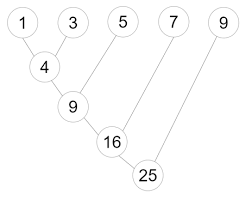
\includegraphics{images/reduce.png}

\texttt{reduce}函数在\texttt{functools}模块中,模块我们后面会讲。要引入\texttt{reduce}函数,使用这行代码:

\texttt{from\ functools\ import\ reduce}

\begin{Shaded}
\begin{Highlighting}[]
\ImportTok{from}\NormalTok{ functools }\ImportTok{import} \BuiltInTok{reduce}
\NormalTok{a }\OperatorTok{=}\NormalTok{ [}\DecValTok{1}\NormalTok{,}\DecValTok{3}\NormalTok{,}\DecValTok{5}\NormalTok{,}\DecValTok{7}\NormalTok{,}\DecValTok{9}\NormalTok{]}

\BuiltInTok{reduce}\NormalTok{(add,a)}
\end{Highlighting}
\end{Shaded}

\begin{verbatim}
25
\end{verbatim}

\hypertarget{ux95edux5305closureux8fdbux9636}{%
\subsection{闭包Closure(进阶)}\label{ux95edux5305closureux8fdbux9636}}

一个闭包closure,可以认为是一个函数,但除了函数体本身,包含了定义闭包时的数据。

例如

\begin{Shaded}
\begin{Highlighting}[]
\KeywordTok{def}\NormalTok{ make\_power\_funcion(n):}
    \KeywordTok{def}\NormalTok{ func(x):}
        \CommentTok{\# return power(x, n) \# 也是一样的}
        \ControlFlowTok{return}\NormalTok{ x }\OperatorTok{**}\NormalTok{ n }
    
    \ControlFlowTok{return}\NormalTok{ func}
\end{Highlighting}
\end{Shaded}

这个代码里,调用\texttt{power()}函数,会返回另一个函数\texttt{fun()}。

这个函数里面调用了变量\texttt{n},但\texttt{n}不在\texttt{fun()}的函数体内,而在上一层。\texttt{fun()}函数,会把生产自己的坏境中的变量(本例中即\texttt{n}),也包括在里面:\textbf{闭包是一个附带数据的函数}。

这段代码发生了什么?

\begin{Shaded}
\begin{Highlighting}[]
\NormalTok{square }\OperatorTok{=}\NormalTok{ make\_power\_funcion(}\DecValTok{2}\NormalTok{) }
\end{Highlighting}
\end{Shaded}

\texttt{square}函数,相当于一个\textbf{附带了\texttt{n=2}的\texttt{func()}函数}

\begin{enumerate}
\def\labelenumi{\arabic{enumi}.}
\tightlist
\item
  \texttt{power(n\ =\ 2)},其中\texttt{n\ =\ 2}
\item
  在\texttt{make\_power\_funcion()}函数的内部,\texttt{func(x)}是可以看见这个\texttt{n=2}的
\item
  \texttt{return\ func}的时候,会把\texttt{n=2},一并返回到外层
\item
  \texttt{square\ =\ power(2)},此时我们把\texttt{square}这个名字,绑定给\texttt{func}这个函数(闭包),而后者同时还附带了\texttt{n=2}
\end{enumerate}

前面讲变量作用域,python找一个名称,是从内到外

\begin{enumerate}
\def\labelenumi{\arabic{enumi}.}
\tightlist
\item
  L局部作用域:即函数体内。例如本例中\texttt{func}函数的\texttt{x}
\item
  Enclosing function
  locals:函数中嵌套函数的外部:例如本例中\texttt{func}函数的\texttt{n}
\item
  G全局:代码的最外层
\item
  B内置名称:python的一些内置的名称,如\texttt{max}函数
\end{enumerate}

现在可知,python查找变量名,先找局部作用域(函数内部),再找闭包的附带数据,再找全局变量,再找python的内置名称。

\hypertarget{ux57faux672cux6570ux636eux7ed3ux6784ux8fdbux9636}{%
\chapter{基本数据结构:进阶}\label{ux57faux672cux6570ux636eux7ed3ux6784ux8fdbux9636}}

前面介绍了常用数据结构的构建,读写数据和遍历等等,这里介绍一些关于数据结构的进阶用法。

\hypertarget{ux5d4cux5957ux6570ux636eux7ed3ux6784}{%
\section{嵌套数据结构}\label{ux5d4cux5957ux6570ux636eux7ed3ux6784}}

数据结构可以相互嵌套。比如List嵌套List,后面我们会知道这是表示矩阵的一种方式。

\begin{Shaded}
\begin{Highlighting}[]
\NormalTok{a }\OperatorTok{=}\NormalTok{ [[}\DecValTok{1}\NormalTok{,}\DecValTok{2}\NormalTok{,}\DecValTok{3}\NormalTok{],[}\DecValTok{3}\NormalTok{,}\DecValTok{5}\NormalTok{,}\DecValTok{1}\NormalTok{],[}\DecValTok{6}\NormalTok{,}\DecValTok{4}\NormalTok{,}\DecValTok{2}\NormalTok{]] }\CommentTok{\# List of List}
\NormalTok{a[}\DecValTok{0}\NormalTok{] }
\end{Highlighting}
\end{Shaded}

\begin{verbatim}
[1, 2, 3]
\end{verbatim}

List嵌套Tuple:

\begin{Shaded}
\begin{Highlighting}[]
\NormalTok{b }\OperatorTok{=}\NormalTok{ [(}\StringTok{\textquotesingle{}A\textquotesingle{}}\NormalTok{,}\DecValTok{2}\NormalTok{),(}\StringTok{\textquotesingle{}B\textquotesingle{}}\NormalTok{,}\DecValTok{3}\NormalTok{),(}\StringTok{\textquotesingle{}C\textquotesingle{}}\NormalTok{,}\DecValTok{1}\NormalTok{)]}
\NormalTok{b[}\DecValTok{2}\NormalTok{]}
\end{Highlighting}
\end{Shaded}

\begin{verbatim}
('C', 1)
\end{verbatim}

字典嵌套 List和Tuple:

\begin{Shaded}
\begin{Highlighting}[]
\NormalTok{c }\OperatorTok{=}\NormalTok{ \{}\StringTok{\textquotesingle{}A\textquotesingle{}}\NormalTok{:[}\DecValTok{1}\NormalTok{,}\DecValTok{2}\NormalTok{,}\DecValTok{3}\NormalTok{],}\StringTok{\textquotesingle{}B\textquotesingle{}}\NormalTok{:(}\DecValTok{3}\NormalTok{,}\DecValTok{4}\NormalTok{,}\DecValTok{5}\NormalTok{),}\StringTok{\textquotesingle{}C\textquotesingle{}}\NormalTok{:[}\DecValTok{2}\NormalTok{,}\DecValTok{3}\NormalTok{,}\DecValTok{4}\NormalTok{]\}}
\NormalTok{c[}\StringTok{\textquotesingle{}B\textquotesingle{}}\NormalTok{]}
\end{Highlighting}
\end{Shaded}

\begin{verbatim}
(3, 4, 5)
\end{verbatim}

当然嵌套可以多层嵌套下去。

嵌套的数据结构,其取值的方法也和原来一样,按照索引或者key逐级排列即可。

\begin{Shaded}
\begin{Highlighting}[]
\NormalTok{a[}\DecValTok{0}\NormalTok{][}\DecValTok{1}\NormalTok{]}
\end{Highlighting}
\end{Shaded}

\begin{verbatim}
2
\end{verbatim}

\begin{Shaded}
\begin{Highlighting}[]
\NormalTok{b[}\DecValTok{1}\NormalTok{][}\DecValTok{0}\NormalTok{]}
\end{Highlighting}
\end{Shaded}

\begin{verbatim}
'B'
\end{verbatim}

\begin{Shaded}
\begin{Highlighting}[]
\NormalTok{c[}\StringTok{\textquotesingle{}B\textquotesingle{}}\NormalTok{][}\DecValTok{1}\NormalTok{]}
\end{Highlighting}
\end{Shaded}

\begin{verbatim}
4
\end{verbatim}

\hypertarget{ux6392ux5e8fux4e13ux9898}{%
\section{排序专题}\label{ux6392ux5e8fux4e13ux9898}}

\hypertarget{ux5217ux8868}{%
\subsection{列表}\label{ux5217ux8868}}

列表的排序很简单

\begin{enumerate}
\def\labelenumi{\arabic{enumi}.}
\tightlist
\item
  \texttt{sorted()}函数返回一个排序后的新列表,原列表不变。
\item
  列表的\texttt{.sort()}方法,对原列表进行``原地排序'',不返回值,但原列表会改变。
\end{enumerate}

\begin{Shaded}
\begin{Highlighting}[]
\NormalTok{a }\OperatorTok{=}\NormalTok{ [}\DecValTok{3}\NormalTok{,}\DecValTok{2}\NormalTok{,}\DecValTok{1}\NormalTok{,}\DecValTok{5}\NormalTok{]}
\end{Highlighting}
\end{Shaded}

\begin{Shaded}
\begin{Highlighting}[]
\BuiltInTok{print}\NormalTok{(}\BuiltInTok{sorted}\NormalTok{(a)) }\CommentTok{\#返回排序后的新列表}
\BuiltInTok{print}\NormalTok{(a) }\CommentTok{\# 注意sorted函数不会改变a}
\end{Highlighting}
\end{Shaded}

\begin{verbatim}
[1, 2, 3, 5]
[3, 2, 1, 5]
\end{verbatim}

\begin{Shaded}
\begin{Highlighting}[]
\NormalTok{a.sort() }\CommentTok{\# 原地排序,会改变a}
\BuiltInTok{print}\NormalTok{(a)}
\end{Highlighting}
\end{Shaded}

\begin{verbatim}
[1, 2, 3, 5]
\end{verbatim}

逆序的话,需要加入\texttt{reverse=True}参数。

\begin{Shaded}
\begin{Highlighting}[]
\NormalTok{a }\OperatorTok{=}\NormalTok{ [}\DecValTok{2}\NormalTok{,}\DecValTok{5}\NormalTok{,}\DecValTok{1}\NormalTok{,}\DecValTok{3}\NormalTok{]}

\BuiltInTok{print}\NormalTok{(}\BuiltInTok{sorted}\NormalTok{(a,reverse}\OperatorTok{=}\VariableTok{True}\NormalTok{)) }\CommentTok{\# 逆序,sorted返回一个排序好的新列表,不改变原值}
\BuiltInTok{print}\NormalTok{(a) }\CommentTok{\# a保持不变}
\NormalTok{a.sort(reverse}\OperatorTok{=}\VariableTok{True}\NormalTok{) }\CommentTok{\# 逆序,原地排序,这个方法不返回值。}
\BuiltInTok{print}\NormalTok{(a) }\CommentTok{\# a已经被改变}
\end{Highlighting}
\end{Shaded}

\begin{verbatim}
[5, 3, 2, 1]
[2, 5, 1, 3]
[5, 3, 2, 1]
\end{verbatim}

\hypertarget{ux4efbux610fux6392ux5e8fux89c4ux5219}{%
\subsection{任意排序规则}\label{ux4efbux610fux6392ux5e8fux89c4ux5219}}

对于嵌套数据结构和字典等等,我们可以构造任意的排序规则。例如,一个嵌套的List:

\begin{Shaded}
\begin{Highlighting}[]
\NormalTok{a }\OperatorTok{=}\NormalTok{ [[}\StringTok{\textquotesingle{}C\textquotesingle{}}\NormalTok{,}\DecValTok{1}\NormalTok{,}\DecValTok{2}\NormalTok{],[}\StringTok{\textquotesingle{}A\textquotesingle{}}\NormalTok{,}\DecValTok{3}\NormalTok{,}\DecValTok{1}\NormalTok{],[}\StringTok{\textquotesingle{}B\textquotesingle{}}\NormalTok{,}\DecValTok{2}\NormalTok{,}\DecValTok{6}\NormalTok{]]}
\NormalTok{a}
\end{Highlighting}
\end{Shaded}

\begin{verbatim}
[['C', 1, 2], ['A', 3, 1], ['B', 2, 6]]
\end{verbatim}

我们想根据每个子List的第二个元素来排序,需要用到参数\texttt{key}(上面两种排序方法都适用)

\begin{enumerate}
\def\labelenumi{\arabic{enumi}.}
\tightlist
\item
  \texttt{key}参数接受一个函数
\item
  这个函数接受List的一个元素,返回一个''可以比较大小的值''(比如一个数字)。
\end{enumerate}

换句话说,你给出一个排序的凭据,要构造一个比较不同子List大小办法,这个办法的结果,体现在你要算出一个可比较的值,如一个数字。

落实到本例,如果只是比较第二个元素的大小,则直接返回第二个元素即可。

\begin{Shaded}
\begin{Highlighting}[]
\KeywordTok{def}\NormalTok{ get\_2nd\_item(x):}
    \ControlFlowTok{return}\NormalTok{ x[}\DecValTok{1}\NormalTok{]}

\BuiltInTok{sorted}\NormalTok{(a, key }\OperatorTok{=}\NormalTok{ get\_2nd\_item)}
\end{Highlighting}
\end{Shaded}

\begin{verbatim}
[['C', 1, 2], ['B', 2, 6], ['A', 3, 1]]
\end{verbatim}

也可以采用匿名函数,见前面的章节。

\begin{Shaded}
\begin{Highlighting}[]
\CommentTok{\# 写成匿名函数的版本}
\BuiltInTok{sorted}\NormalTok{(a, key }\OperatorTok{=} \KeywordTok{lambda}\NormalTok{ x:x[}\DecValTok{1}\NormalTok{]) }
\end{Highlighting}
\end{Shaded}

\begin{verbatim}
[['C', 1, 2], ['B', 2, 6], ['A', 3, 1]]
\end{verbatim}

有如,比如你要根据
``第2和第3个元素的和''来排序,你只要构造一个函数,返回这两者的和即可。

\begin{Shaded}
\begin{Highlighting}[]
\KeywordTok{def}\NormalTok{ sum\_2\_3(x):}
    \ControlFlowTok{return}\NormalTok{ x[}\DecValTok{1}\NormalTok{]}\OperatorTok{+}\NormalTok{x[}\DecValTok{2}\NormalTok{]}

\BuiltInTok{print}\NormalTok{(a[}\DecValTok{0}\NormalTok{]) }\CommentTok{\# 测试一下是否正常}

\BuiltInTok{sorted}\NormalTok{(a, key }\OperatorTok{=}\NormalTok{ sum\_2\_3)}
\end{Highlighting}
\end{Shaded}

\begin{verbatim}
['C', 1, 2]
\end{verbatim}

\begin{verbatim}
[['C', 1, 2], ['A', 3, 1], ['B', 2, 6]]
\end{verbatim}

\begin{Shaded}
\begin{Highlighting}[]
\CommentTok{\# 写成匿名函数的版本}
\BuiltInTok{sorted}\NormalTok{(a, key }\OperatorTok{=} \KeywordTok{lambda}\NormalTok{ x:x[}\DecValTok{1}\NormalTok{]}\OperatorTok{+}\NormalTok{x[}\DecValTok{2}\NormalTok{])}
\end{Highlighting}
\end{Shaded}

\begin{verbatim}
[['C', 1, 2], ['A', 3, 1], ['B', 2, 6]]
\end{verbatim}

\hypertarget{ux5b57ux5178ux6392ux5e8f}{%
\subsection{字典排序}\label{ux5b57ux5178ux6392ux5e8f}}

前面说过,字典大约也可以``看成''一个嵌套数据结构,以前面的字典c为例

\begin{Shaded}
\begin{Highlighting}[]
\NormalTok{c.items()}
\end{Highlighting}
\end{Shaded}

\begin{verbatim}
dict_items([('A', [1, 2, 3]), ('B', (3, 4, 5)), ('C', [2, 3, 4])])
\end{verbatim}

注意到value是一个3个元素的List或者Tuple,我们要根据value的第一个元素来排序。

\begin{Shaded}
\begin{Highlighting}[]
\NormalTok{sorted\_items }\OperatorTok{=} \BuiltInTok{sorted}\NormalTok{(c.items(), key}\OperatorTok{=} \KeywordTok{lambda}\NormalTok{ x:x[}\DecValTok{1}\NormalTok{][}\DecValTok{0}\NormalTok{])}
\NormalTok{sorted\_items}
\end{Highlighting}
\end{Shaded}

\begin{verbatim}
[('A', [1, 2, 3]), ('C', [2, 3, 4]), ('B', (3, 4, 5))]
\end{verbatim}

注意,其中x是一个字典中的item,即一个(key,value)对。那么x{[}0{]}就是key,x{[}1{]}就是value,x{[}1{]}{[}0{]}就是value中的第一个元素了。

注意上面得到的是一个List of
Tuple,即单纯的嵌套数据结构。如果需要转为字典,调用dict()函数即可(简单类型转换)

\begin{Shaded}
\begin{Highlighting}[]
\BuiltInTok{dict}\NormalTok{(}\BuiltInTok{sorted}\NormalTok{(c.items(), key}\OperatorTok{=} \KeywordTok{lambda}\NormalTok{ x:x[}\DecValTok{1}\NormalTok{][}\DecValTok{0}\NormalTok{]))}
\end{Highlighting}
\end{Shaded}

\begin{verbatim}
{'A': [1, 2, 3], 'C': [2, 3, 4], 'B': (3, 4, 5)}
\end{verbatim}

\hypertarget{ux5176ux4ed6-1}{%
\section{其他}\label{ux5176ux4ed6-1}}

\hypertarget{ux679aux4e3e-enumerateux51fdux6570}{%
\subsection{枚举
enumerate函数}\label{ux679aux4e3e-enumerateux51fdux6570}}

\texttt{enumerate()}函数一般用于遍历一个可迭代对象的时候,同时还可以获得对应的索引。

或者说,你遍历一个a\_list =
{[}`a',`b',`c'{]}的时候,还想获得当前值是``第几个'',我们用以下循环

\texttt{for\ i,value\ in\ enumerate(a\_list):}

\begin{Shaded}
\begin{Highlighting}[]
\NormalTok{a\_list }\OperatorTok{=} \BuiltInTok{list}\NormalTok{(}\StringTok{\textquotesingle{}apple\textquotesingle{}}\NormalTok{)}

\ControlFlowTok{for}\NormalTok{ i,value }\KeywordTok{in} \BuiltInTok{enumerate}\NormalTok{(a\_list):}
    \BuiltInTok{print}\NormalTok{(i,value) }\CommentTok{\# 此时,i就表示遍历过程中的索引}
\end{Highlighting}
\end{Shaded}

\begin{verbatim}
0 a
1 p
2 p
3 l
4 e
\end{verbatim}

显然,和字典\texttt{.items()}类似,\texttt{enumerate(a\_list)}也是获得可以
\texttt{{[}(index,\ value),\ (index,\ value),\ ...{]}}的序列。

注:\texttt{enumerate(a\_list)}返回一个生成器,当你要具体访问里面的值的时候,才会临时生成某个\texttt{(index,value)},如果要打印出来看,需要转为List。(当然也可以转为字典)

\begin{Shaded}
\begin{Highlighting}[]
\CommentTok{\# 把a\_list,转为带有索引的list}
\BuiltInTok{print}\NormalTok{(}\BuiltInTok{list}\NormalTok{(}\BuiltInTok{enumerate}\NormalTok{(a\_list)))}

\CommentTok{\# 把a\_list,转为以index为key的字典}
\BuiltInTok{print}\NormalTok{(}\BuiltInTok{dict}\NormalTok{(}\BuiltInTok{enumerate}\NormalTok{(a\_list)))}
\end{Highlighting}
\end{Shaded}

\begin{verbatim}
[(0, 'a'), (1, 'p'), (2, 'p'), (3, 'l'), (4, 'e')]
{0: 'a', 1: 'p', 2: 'p', 3: 'l', 4: 'e'}
\end{verbatim}

进一步,可以获得``某个元素的索引'',比如问'p'是几号元素?

\begin{Shaded}
\begin{Highlighting}[]
\NormalTok{a\_list }\OperatorTok{=} \BuiltInTok{list}\NormalTok{(}\StringTok{\textquotesingle{}apple\textquotesingle{}}\NormalTok{)}
\NormalTok{[i }\ControlFlowTok{for}\NormalTok{ i,value }\KeywordTok{in} \BuiltInTok{enumerate}\NormalTok{(a\_list) }\ControlFlowTok{if}\NormalTok{ value }\OperatorTok{==} \StringTok{\textquotesingle{}p\textquotesingle{}}\NormalTok{]}
\end{Highlighting}
\end{Shaded}

\begin{verbatim}
[1, 2]
\end{verbatim}

\hypertarget{zipux51fdux6570}{%
\subsection{zip函数}\label{zipux51fdux6570}}

把几个序列结构,每个元素对位组合,形成一个Tuple,再组成一个List。

注意:zip以最短的元素为主。

\begin{Shaded}
\begin{Highlighting}[]
\NormalTok{list1}\OperatorTok{=}\NormalTok{ (}\StringTok{\textquotesingle{}a\textquotesingle{}}\NormalTok{, }\StringTok{\textquotesingle{}b\textquotesingle{}}\NormalTok{, }\StringTok{\textquotesingle{}c\textquotesingle{}}\NormalTok{)}
\NormalTok{list2 }\OperatorTok{=}\NormalTok{ [}\DecValTok{1}\NormalTok{, }\DecValTok{2}\NormalTok{, }\DecValTok{3}\NormalTok{, }\DecValTok{4}\NormalTok{]}

\BuiltInTok{print}\NormalTok{(}\BuiltInTok{list}\NormalTok{(}\BuiltInTok{zip}\NormalTok{(list1,list2)))}
\BuiltInTok{print}\NormalTok{(}\BuiltInTok{list}\NormalTok{(}\BuiltInTok{zip}\NormalTok{(list1,list2,list1))) }\CommentTok{\# 可以组合不止2个序列}
\end{Highlighting}
\end{Shaded}

\begin{verbatim}
[('a', 1), ('b', 2), ('c', 3)]
[('a', 1, 'a'), ('b', 2, 'b'), ('c', 3, 'c')]
\end{verbatim}

稍微发散一下,这不就是一个Dict的结构吗?所以可以直接转为字典。

\begin{Shaded}
\begin{Highlighting}[]
\BuiltInTok{dict}\NormalTok{(}\BuiltInTok{zip}\NormalTok{(list1,list2))}
\end{Highlighting}
\end{Shaded}

\begin{verbatim}
{'a': 1, 'b': 2, 'c': 3}
\end{verbatim}

当然也可以多序列循环

\begin{Shaded}
\begin{Highlighting}[]
\ControlFlowTok{for}\NormalTok{ i,j }\KeywordTok{in} \BuiltInTok{zip}\NormalTok{(list1,list2):}
    \BuiltInTok{print}\NormalTok{(i,j)}
\end{Highlighting}
\end{Shaded}

\begin{verbatim}
a 1
b 2
c 3
\end{verbatim}

回忆函数的拆包操作,我把一个List(等)传递给一个函数,前面加一个*,就会自动把List中的元素逐一拆出来,传递给函数。

\begin{Shaded}
\begin{Highlighting}[]
\KeywordTok{def}\NormalTok{ add(a,b):}
    \ControlFlowTok{return}\NormalTok{ a }\OperatorTok{+}\NormalTok{ b}

\NormalTok{add(}\OperatorTok{*}\NormalTok{[}\DecValTok{1}\NormalTok{,}\DecValTok{2}\NormalTok{]) }\CommentTok{\# 对[1,2]进行拆包:按顺序传递给a和b}
\end{Highlighting}
\end{Shaded}

\begin{verbatim}
3
\end{verbatim}

对于zip函数也可以这样做,比如你有一个序列

\texttt{a\_list\ =\ {[}(1,\ \textquotesingle{}one\textquotesingle{}),\ (2,\ \textquotesingle{}two\textquotesingle{}),\ (3,\ \textquotesingle{}three\textquotesingle{}){]}}

你希望第一位的元素组成序列,第二位的元素组成一个序列\ldots.

\begin{Shaded}
\begin{Highlighting}[]
\NormalTok{a\_list }\OperatorTok{=}\NormalTok{ [(}\DecValTok{1}\NormalTok{, }\StringTok{\textquotesingle{}one\textquotesingle{}}\NormalTok{), (}\DecValTok{2}\NormalTok{, }\StringTok{\textquotesingle{}two\textquotesingle{}}\NormalTok{), (}\DecValTok{3}\NormalTok{, }\StringTok{\textquotesingle{}three\textquotesingle{}}\NormalTok{)]}
\BuiltInTok{list}\NormalTok{(}\BuiltInTok{zip}\NormalTok{(}\OperatorTok{*}\NormalTok{a\_list))}
\end{Highlighting}
\end{Shaded}

\begin{verbatim}
[(1, 2, 3), ('one', 'two', 'three')]
\end{verbatim}

\begin{Shaded}
\begin{Highlighting}[]
\NormalTok{x,y }\OperatorTok{=} \BuiltInTok{list}\NormalTok{(}\BuiltInTok{zip}\NormalTok{(}\OperatorTok{*}\NormalTok{a\_list)) }\CommentTok{\# 如果要赋值的话,可以这么写}
\end{Highlighting}
\end{Shaded}

\hypertarget{popux51fdux6570}{%
\subsection{pop函数}\label{popux51fdux6570}}

\texttt{pop()}函数用于``返回并移除一个元素'',近似理解就是把队尾的一个元素``拿出来''。

对于List,默认是最后一个元素(队尾)。

\begin{Shaded}
\begin{Highlighting}[]
\NormalTok{a }\OperatorTok{=} \BuiltInTok{list}\NormalTok{(}\StringTok{\textquotesingle{}apple\textquotesingle{}}\NormalTok{)}

\BuiltInTok{print}\NormalTok{(a.pop()) }\CommentTok{\# 获取最后个元素,并删除。}
\BuiltInTok{print}\NormalTok{(a) }\CommentTok{\# 最后一个元素已经删除}
\end{Highlighting}
\end{Shaded}

\begin{verbatim}
e
['a', 'p', 'p', 'l']
\end{verbatim}

也可以指定index,比如拿出1号元素。

\begin{Shaded}
\begin{Highlighting}[]
\BuiltInTok{print}\NormalTok{(a.pop(}\DecValTok{1}\NormalTok{))}
\BuiltInTok{print}\NormalTok{(a)}
\end{Highlighting}
\end{Shaded}

\begin{verbatim}
p
['a', 'p', 'l']
\end{verbatim}

对于Dic,需要指定key,pop()会返回value,并移除这个key。

\begin{Shaded}
\begin{Highlighting}[]
\NormalTok{b }\OperatorTok{=}\NormalTok{ \{}\StringTok{\textquotesingle{}a\textquotesingle{}}\NormalTok{: }\DecValTok{1}\NormalTok{, }\StringTok{\textquotesingle{}b\textquotesingle{}}\NormalTok{: }\DecValTok{2}\NormalTok{, }\StringTok{\textquotesingle{}c\textquotesingle{}}\NormalTok{: }\DecValTok{3}\NormalTok{\}}

\BuiltInTok{print}\NormalTok{(b.pop(}\StringTok{\textquotesingle{}b\textquotesingle{}}\NormalTok{)) }\CommentTok{\# 获取\textquotesingle{}b\textquotesingle{}对应的value,并删除\textquotesingle{}b\textquotesingle{}。}
\BuiltInTok{print}\NormalTok{(b) }\CommentTok{\# \textquotesingle{}b\textquotesingle{}已经删除}
\end{Highlighting}
\end{Shaded}

\begin{verbatim}
2
{'a': 1, 'c': 3}
\end{verbatim}

\hypertarget{ux66f4ux591aux7ec3ux4e60-1}{%
\section{更多练习}\label{ux66f4ux591aux7ec3ux4e60-1}}

以下是同学的姓名,学号和考试分数的数据

\begin{verbatim}
names = ["Alice", "Bob", "Clare"]
ids = [101,102,103]
scores = [85, 92, 78]
\end{verbatim}

\begin{enumerate}
\def\labelenumi{\arabic{enumi}.}
\tightlist
\item
  构建一个字典data,其中key是名字,value是另一个字典key和value是id和score以及对应的值。
\end{enumerate}

构建出来大概是这样:
\texttt{\{\textquotesingle{}Alice\textquotesingle{}:\ \{\textquotesingle{}id\textquotesingle{}:\ 1,\ \textquotesingle{}score\textquotesingle{}:\ 85\},\ \ ...\}}

\begin{enumerate}
\def\labelenumi{\arabic{enumi}.}
\setcounter{enumi}{1}
\item
  对data按分数排序,高分的在前面。
\item
  找出分数最高的同学,打印``分数最高的同学是: ??? ,学号是???,分数是:
  ???。''
\end{enumerate}

\hypertarget{ux5206ux6790ux8fc7ux7a0bux8303ux4f8b}{%
\chapter{分析过程范例}\label{ux5206ux6790ux8fc7ux7a0bux8303ux4f8b}}

\hypertarget{ux6570ux636eux6d41ux5982ux4f55ux7ec4ux7ec7ux4f60ux7684ux4ee3ux7801}{%
\section{数据流:如何组织你的代码}\label{ux6570ux636eux6d41ux5982ux4f55ux7ec4ux7ec7ux4f60ux7684ux4ee3ux7801}}

如何设计的一个分析过程?我们继续用前面榨汁机的例子。

把一个苹果变成苹果汁,假定要3个步骤:

\begin{enumerate}
\def\labelenumi{\arabic{enumi}.}
\tightlist
\item
  削皮
\item
  切块
\item
  榨汁
\end{enumerate}

如果我们把每个过程看成一个函数,大概是这样的:

\begin{verbatim}
削了皮的苹果 = 削皮(苹果) 
苹果块 = 切块(削了皮的苹果) 
苹果汁 = 榨汁(苹果块) 
\end{verbatim}

我们换一个方式可能看得更清楚一点:

\begin{verbatim}

苹果 ─┐
削皮(苹果) ───────┐
        切块(削了皮的苹果) ─────┐
                        榨汁(苹果块) ──┐ 
                                    苹果汁
\end{verbatim}

其中每一个过程,比如削皮,可能是一个函数,也可能是无数代码组成的模块。
我们编写分析流程的整体,以及每一个模块内部,也是呈现同样的结构。

如果有参数呢?比如切块的时候切成5块,用榨汁的时候用3档速度:

可以把数据流(苹果 -\textgreater{} 削了皮的苹果 -\textgreater{}
苹果块)放在第1个参数位,处理数据的参数放在第二个参数位以后:

\begin{verbatim}
苹果 ─┐
削皮(苹果) ───────┐
      切块(削了皮的苹果, 5块, ... ) ─────┐
                                  榨汁(苹果块, 3档转速, ...) ──┐ 
                                                            苹果汁
\end{verbatim}

因此:

\begin{enumerate}
\def\labelenumi{\arabic{enumi}.}
\tightlist
\item
  分析的流程一般呈现一种数据流的结构:
  每一个步骤,有上游数据的流入(参数),形成新的数据(返回值),成为下游数据流入(参数)。
\item
  如果写成函数,(\textbf{推荐但非必须})第一个参数应该是数据,处理数据的参数可以放在第二位之后。
  如果所有的函数都呈现这种结构,你就会形成一直数据流的直觉。
\item
  每个功能模块(\textbf{尽量})写成纯函数:从参数中接受输入(不读取全局变量,避免被意外改变),
  返回新的数据(尽量但不直接改变函数体外的事物),详见前面的函数式编程。
\end{enumerate}

\hypertarget{ux4eceux6570ux636eux5f00ux59cb}{%
\section{从数据开始}\label{ux4eceux6570ux636eux5f00ux59cb}}

例如,我们要一个程序来处理班级同学的信息。每个同学起码有这几个信息:

\begin{enumerate}
\def\labelenumi{\arabic{enumi}.}
\tightlist
\item
  学号
\item
  姓名
\item
  专业
\item
  班级号
\end{enumerate}

表示1个同学:

用现在所学的信息(人的属性),一般可以表示成key:value结构,所以我们可以用字典dict来表示任何一个同学。
(当然方法很多,后面会学到)

\begin{Shaded}
\begin{Highlighting}[]
\NormalTok{student\_1 }\OperatorTok{=}\NormalTok{ \{}\StringTok{\textquotesingle{}student\_id\textquotesingle{}}\NormalTok{:}\DecValTok{2021001}\NormalTok{, }\StringTok{\textquotesingle{}name\textquotesingle{}}\NormalTok{:}\StringTok{\textquotesingle{}Alex\textquotesingle{}}\NormalTok{, }\StringTok{\textquotesingle{}major\textquotesingle{}}\NormalTok{: }\StringTok{\textquotesingle{}finance\textquotesingle{}}\NormalTok{, }\StringTok{\textquotesingle{}class\_id\textquotesingle{}}\NormalTok{:}\DecValTok{1}\NormalTok{\}}
\NormalTok{student\_2 }\OperatorTok{=}\NormalTok{ \{}\StringTok{\textquotesingle{}student\_id\textquotesingle{}}\NormalTok{:}\DecValTok{2021002}\NormalTok{, }\StringTok{\textquotesingle{}name\textquotesingle{}}\NormalTok{:}\StringTok{\textquotesingle{}Bob\textquotesingle{}}\NormalTok{, }\StringTok{\textquotesingle{}major\textquotesingle{}}\NormalTok{: }\StringTok{\textquotesingle{}finance\textquotesingle{}}\NormalTok{, }\StringTok{\textquotesingle{}class\_id\textquotesingle{}}\NormalTok{:}\DecValTok{1}\NormalTok{\}}
\NormalTok{student\_3 }\OperatorTok{=}\NormalTok{ \{}\StringTok{\textquotesingle{}student\_id\textquotesingle{}}\NormalTok{:}\DecValTok{2021003}\NormalTok{, }\StringTok{\textquotesingle{}name\textquotesingle{}}\NormalTok{:}\StringTok{\textquotesingle{}Clare\textquotesingle{}}\NormalTok{, }\StringTok{\textquotesingle{}major\textquotesingle{}}\NormalTok{: }\StringTok{\textquotesingle{}accounting\textquotesingle{}}\NormalTok{, }\StringTok{\textquotesingle{}class\_id\textquotesingle{}}\NormalTok{:}\DecValTok{2}\NormalTok{\}}


\BuiltInTok{print}\NormalTok{(student\_1[}\StringTok{\textquotesingle{}student\_id\textquotesingle{}}\NormalTok{])}
\BuiltInTok{print}\NormalTok{(student\_2[}\StringTok{\textquotesingle{}name\textquotesingle{}}\NormalTok{])}
\BuiltInTok{print}\NormalTok{(student\_3[}\StringTok{\textquotesingle{}major\textquotesingle{}}\NormalTok{])}
\end{Highlighting}
\end{Shaded}

\begin{verbatim}
2021001
Bob
accounting
\end{verbatim}

表示所有同学:

组织一堆同类数据:List(或者另一个Dict,如果需要一个索引如学号,见作业)。

\begin{Shaded}
\begin{Highlighting}[]
\CommentTok{\# List版本}

\NormalTok{students\_info }\OperatorTok{=}\NormalTok{ [}
\NormalTok{  student\_1,}
\NormalTok{  student\_2,}
\NormalTok{  student\_3}
\NormalTok{]}

\BuiltInTok{print}\NormalTok{(students\_info)}
\end{Highlighting}
\end{Shaded}

\begin{verbatim}
[{'student_id': 2021001, 'name': 'Alex', 'major': 'finance', 'class_id': 1}, {'student_id': 2021002, 'name': 'Bob', 'major': 'finance', 'class_id': 1}, {'student_id': 2021003, 'name': 'Clare', 'major': 'accounting', 'class_id': 2}]
\end{verbatim}

\hypertarget{ux6dfbux52a0ux529fux80fd}{%
\section{添加功能}\label{ux6dfbux52a0ux529fux80fd}}

\hypertarget{ux67e5ux627e}{%
\subsection{查找}\label{ux67e5ux627e}}

显然按条件查找是必须有的功能。

例如:在数据中找一位名叫Alex的同学。

\begin{enumerate}
\def\labelenumi{\arabic{enumi}.}
\tightlist
\item
  既然students\_info是一个列表,那我们就用列表推导式。
\end{enumerate}

\begin{Shaded}
\begin{Highlighting}[]
\NormalTok{result }\OperatorTok{=}\NormalTok{ [s }\ControlFlowTok{for}\NormalTok{ s }\KeywordTok{in}\NormalTok{ students\_info }\ControlFlowTok{if}\NormalTok{ s[}\StringTok{\textquotesingle{}name\textquotesingle{}}\NormalTok{] }\OperatorTok{==} \StringTok{"Alex"}\NormalTok{]}

\BuiltInTok{print}\NormalTok{(result)}
\end{Highlighting}
\end{Shaded}

\begin{verbatim}
[{'student_id': 2021001, 'name': 'Alex', 'major': 'finance', 'class_id': 1}]
\end{verbatim}

注意:列表推导式的结果,也是一个列表,即使其中只有1个元素。看打印的最2边是中括号。

那么有多少个同学叫Alex?

\begin{Shaded}
\begin{Highlighting}[]
\BuiltInTok{len}\NormalTok{(result)}
\end{Highlighting}
\end{Shaded}

\begin{verbatim}
1
\end{verbatim}

那我们可以获得Alex的信息,例如学号和专业

\begin{Shaded}
\begin{Highlighting}[]
\BuiltInTok{print}\NormalTok{(result[}\DecValTok{0}\NormalTok{][}\StringTok{\textquotesingle{}student\_id\textquotesingle{}}\NormalTok{])}
\BuiltInTok{print}\NormalTok{(result[}\DecValTok{0}\NormalTok{][}\StringTok{\textquotesingle{}major\textquotesingle{}}\NormalTok{])}
\end{Highlighting}
\end{Shaded}

\begin{verbatim}
2021001
finance
\end{verbatim}

按人名查找,是一个特别常用的功能,那我们把这个功能写成一个函数:

\begin{Shaded}
\begin{Highlighting}[]
\KeywordTok{def}\NormalTok{ find\_students\_by\_name(data, name):}
    \CommentTok{"""}
\CommentTok{    按姓名查找同学。}

\CommentTok{    参数:}
\CommentTok{        data: 保存所有同学信息的数据List[dict]}
\CommentTok{        name: 目标的姓名}
\CommentTok{    返回值:}
\CommentTok{        return: 返回同名同学的List。如果找不到则返回[]。}
\CommentTok{    """}
\NormalTok{    result }\OperatorTok{=}\NormalTok{ [s }\ControlFlowTok{for}\NormalTok{ s }\KeywordTok{in}\NormalTok{ data }\ControlFlowTok{if}\NormalTok{ s[}\StringTok{\textquotesingle{}name\textquotesingle{}}\NormalTok{] }\OperatorTok{==}\NormalTok{ name]}
    \ControlFlowTok{return}\NormalTok{ result}

\NormalTok{result }\OperatorTok{=}\NormalTok{ find\_students\_by\_name(students\_info,}\StringTok{"Alex"}\NormalTok{)}
\BuiltInTok{print}\NormalTok{(result)}
\end{Highlighting}
\end{Shaded}

\begin{verbatim}
[{'student_id': 2021001, 'name': 'Alex', 'major': 'finance', 'class_id': 1}]
\end{verbatim}

为什么要把一个过程写成一个函数?

\begin{enumerate}
\def\labelenumi{\arabic{enumi}.}
\tightlist
\item
  常用:don't repeat
  yourself。常用的代码推荐包装起来,起一个顾名思义的名字。
\item
  复杂的代码:编写良好的函数,可以让你关注于接口和功能(函数名、参数、返回值):你按一下遥控,电视机就会开,中间的过程你完全不想知道。
\end{enumerate}

\hypertarget{ux7ec3ux4e60ux6309ux5b66ux53f7ux67e5ux627e}{%
\subsection{练习:按学号查找}\label{ux7ec3ux4e60ux6309ux5b66ux53f7ux67e5ux627e}}

\begin{enumerate}
\def\labelenumi{\arabic{enumi}.}
\tightlist
\item
  按学号查找,但学号是唯一的,因此逻辑上只能有一个数据。
\item
  因此,获得的数据之后,不返回列表,只返回代表学生的dict。
\item
  如果学号有重复,打印一个警告信息:``学号有重复!请检查!''
\end{enumerate}

\begin{Shaded}
\begin{Highlighting}[]
\KeywordTok{def}\NormalTok{ find\_student\_by\_id(data, student\_id):}
  \CommentTok{\textquotesingle{}\textquotesingle{}\textquotesingle{}}
\CommentTok{  按学号查找同学}
\CommentTok{  \textquotesingle{}\textquotesingle{}\textquotesingle{}}
  \ControlFlowTok{pass} \CommentTok{\# 这部分由你完成}

\NormalTok{result }\OperatorTok{=}\NormalTok{ find\_student\_by\_id(students\_info, }\DecValTok{2021002}\NormalTok{)}
\BuiltInTok{print}\NormalTok{(result)}
\end{Highlighting}
\end{Shaded}

\begin{verbatim}
None
\end{verbatim}

\hypertarget{ux7b80ux5355ux7edfux8ba1}{%
\subsection{简单统计}\label{ux7b80ux5355ux7edfux8ba1}}

统计一下,金融专业有多少人?

\begin{enumerate}
\def\labelenumi{\arabic{enumi}.}
\tightlist
\item
  先筛选(利用上面的知识)
\item
  再算数
\end{enumerate}

\begin{Shaded}
\begin{Highlighting}[]
\NormalTok{finance\_students }\OperatorTok{=}\NormalTok{ [s }\ControlFlowTok{for}\NormalTok{ s }\KeywordTok{in}\NormalTok{ students\_info }\ControlFlowTok{if}\NormalTok{ s[}\StringTok{\textquotesingle{}major\textquotesingle{}}\NormalTok{] }\OperatorTok{==} \StringTok{\textquotesingle{}finance\textquotesingle{}}\NormalTok{]}

\BuiltInTok{len}\NormalTok{(finance\_students)}
\end{Highlighting}
\end{Shaded}

\begin{verbatim}
2
\end{verbatim}

当然,也可以写个2函数:同样,先查找,在统计

\begin{Shaded}
\begin{Highlighting}[]
\KeywordTok{def}\NormalTok{ find\_students\_by\_major(data, major):}
  \CommentTok{\textquotesingle{}\textquotesingle{}\textquotesingle{}}
\CommentTok{  按专业查找同学}
\CommentTok{  \textquotesingle{}\textquotesingle{}\textquotesingle{}}
\NormalTok{  result }\OperatorTok{=}\NormalTok{ [s }\ControlFlowTok{for}\NormalTok{ s }\KeywordTok{in}\NormalTok{ data }\ControlFlowTok{if}\NormalTok{ s[}\StringTok{\textquotesingle{}major\textquotesingle{}}\NormalTok{] }\OperatorTok{==}\NormalTok{ major]}
  \ControlFlowTok{return}\NormalTok{ result}

\KeywordTok{def}\NormalTok{ count\_by\_major(data, majoy):}
  \CommentTok{\textquotesingle{}\textquotesingle{}\textquotesingle{}}
\CommentTok{  计算专业的同学人数}
\CommentTok{  \textquotesingle{}\textquotesingle{}\textquotesingle{}}
\NormalTok{  class\_size }\OperatorTok{=} \BuiltInTok{len}\NormalTok{(find\_students\_by\_major(data,majoy))}
  \ControlFlowTok{return}\NormalTok{ class\_size}

\BuiltInTok{print}\NormalTok{(}\StringTok{\textquotesingle{}金融专业人数:\textquotesingle{}}\NormalTok{, count\_by\_major(students\_info, }\StringTok{\textquotesingle{}finance\textquotesingle{}}\NormalTok{))}
\BuiltInTok{print}\NormalTok{(}\StringTok{\textquotesingle{}会计专业人数:\textquotesingle{}}\NormalTok{, count\_by\_major(students\_info, }\StringTok{\textquotesingle{}accounting\textquotesingle{}}\NormalTok{))}
\end{Highlighting}
\end{Shaded}

\begin{verbatim}
金融专业人数: 2
会计专业人数: 1
\end{verbatim}

小结:

\begin{enumerate}
\def\labelenumi{\arabic{enumi}.}
\tightlist
\item
  ``一位同学''的信息可以用字典Dict:可以用\texttt{student\_id}等标签,来获取该同学信息。
\item
  ``所有同学''的信息可以用列表List:所有同学,可以看作一个有序的队列,自然可以采用List。大量的列表操作,便于我们进行查找、筛选、统计等等。
\item
  常用的操作,可以写成函数。既便于使用,又可以通过函数名得知操作的意图,一目了然。
\item
  函数名,应该顾名思义。函数体的开头,必须写函数的说明,如作用,算法等。
\end{enumerate}

\hypertarget{ux7efcux5408ux7ec3ux4e60}{%
\section{综合练习}\label{ux7efcux5408ux7ec3ux4e60}}

本章的内容,本质上是针对一些基础的信息(三个同学的信息),构造出数据结构(List-Dict),并且添加处理数据的功能(各种函数)。

以下练习,要求你\textbf{继续}这个过程:在上述内容的基础上,添加新的信息和新的功能。

\hypertarget{ux6dfbux52a0pythonux8bfeux5206ux6570}{%
\subsection{添加python课分数}\label{ux6dfbux52a0pythonux8bfeux5206ux6570}}

问题:按学号\texttt{student\_id},添加同学的python课分数\texttt{python\_score}

知识点:List和Dict的赋值,循环或者列表推导式

\begin{enumerate}
\def\labelenumi{\arabic{enumi}.}
\tightlist
\item
  写一个手动版
\item
  写一个函数版
\end{enumerate}

\begin{longtable}[]{@{}llll@{}}
\toprule\noalign{}
& student\_id & name & python\_score \\
\midrule\noalign{}
\endhead
\bottomrule\noalign{}
\endlastfoot
0 & 2021001 & Alex & 86 \\
1 & 2021002 & Bob & 59 \\
2 & 2021003 & Clare & 92 \\
\end{longtable}

思路:

\begin{enumerate}
\def\labelenumi{\arabic{enumi}.}
\tightlist
\item
  ``一个同学''的信息,是以dict的形式保存,因此我们需要给dict添新的key-value。
\item
  回忆:List和Dict都是可变对象,你可以直接对List中的Dict中的key赋值!
\end{enumerate}

\begin{Shaded}
\begin{Highlighting}[]
\KeywordTok{def}\NormalTok{ set\_python\_score(data, student\_id, score):}
  \CommentTok{\textquotesingle{}\textquotesingle{}\textquotesingle{}}
\CommentTok{  设置python课的分数}
\CommentTok{  \textquotesingle{}\textquotesingle{}\textquotesingle{}}
  \ControlFlowTok{pass} \CommentTok{\# 这里由你完成}

\NormalTok{set\_python\_score(students\_info,}\DecValTok{2021001}\NormalTok{,}\DecValTok{90}\NormalTok{)}
\end{Highlighting}
\end{Shaded}

\hypertarget{ux7b80ux5355ux7edfux8ba1-1}{%
\subsection{简单统计}\label{ux7b80ux5355ux7edfux8ba1-1}}

问题:统计python课的所有同学的平均分,以及分班级的平均分。

知识点:循环或者列表推导式,累加,简单计算

\begin{enumerate}
\def\labelenumi{\arabic{enumi}.}
\tightlist
\item
  手动版
\item
  函数版
\end{enumerate}

\begin{Shaded}
\begin{Highlighting}[]
\KeywordTok{def}\NormalTok{ get\_avg\_python\_score(data):}
  \CommentTok{\textquotesingle{}\textquotesingle{}\textquotesingle{}}
\CommentTok{  统计python课的平均分}
\CommentTok{  \textquotesingle{}\textquotesingle{}\textquotesingle{}}
  \ControlFlowTok{pass} \CommentTok{\# 这里由你完成}

\KeywordTok{def}\NormalTok{ get\_avg\_python\_score\_by\_class(data,  class\_id):}
  \CommentTok{\textquotesingle{}\textquotesingle{}\textquotesingle{}}
\CommentTok{  按班级,统计python课的平均分}
\CommentTok{  \textquotesingle{}\textquotesingle{}\textquotesingle{}}
  \ControlFlowTok{pass} \CommentTok{\# 这里由你完成}
\end{Highlighting}
\end{Shaded}

\hypertarget{ux7531ux5206ux6570ux83b7ux5f97ux8bc4ux7ea7}{%
\subsection{由分数获得评级}\label{ux7531ux5206ux6570ux83b7ux5f97ux8bc4ux7ea7}}

问题:按照分数,给同学添加一个\texttt{rank}的变量。

知识点:\texttt{if}条件判断,List和Dict的赋值

\begin{enumerate}
\def\labelenumi{\arabic{enumi}.}
\tightlist
\item
  90分+,``A''
\item
  80分+,``B''
\item
  70分+,``C''
\item
  60分+,``D''
\item
  不足60分,``E''
\end{enumerate}

\hypertarget{ux5224ux65adux662fux5426ux53caux683c}{%
\subsection{判断是否及格}\label{ux5224ux65adux662fux5426ux53caux683c}}

问题:按照分数,给同学添加一个\texttt{pass}的变量。60分以上为及格

知识点:\texttt{if}条件判断,List和Dict的赋值,布尔值

\begin{enumerate}
\def\labelenumi{\arabic{enumi}.}
\tightlist
\item
  手动版
\item
  函数版
\item
  统计及格率
\end{enumerate}

\hypertarget{ux4fe1ux606fux8f93ux51fa}{%
\subsection{信息输出}\label{ux4fe1ux606fux8f93ux51fa}}

问题:以字符串的形式,输出某一个同学的信息(通过学号)

知识点:循环或列表推导式,字符串操作。

\begin{enumerate}
\def\labelenumi{\arabic{enumi}.}
\tightlist
\item
  输出的结果类似: ``学号: ???? ; 姓名:??? ; 班级 ??? \ldots{}
  \ldots{}''。其中,班级信息要输出''专业 班级号''的形式,如``金融 5班''
\item
  手动版
\item
  函数版
\item
  写一个函数,输出不及格的同学的信息
\end{enumerate}

\begin{Shaded}
\begin{Highlighting}[]
\KeywordTok{def}\NormalTok{ print\_by\_student\_id(data, student\_id):}
  \CommentTok{\textquotesingle{}\textquotesingle{}\textquotesingle{}}
\CommentTok{  打印同学信息}
\CommentTok{  \textquotesingle{}\textquotesingle{}\textquotesingle{}}
  \ControlFlowTok{pass} \CommentTok{\# 这里由你完成}

\KeywordTok{def}\NormalTok{ print\_failed(data):}
  \CommentTok{\textquotesingle{}\textquotesingle{}\textquotesingle{}}
\CommentTok{  打印不及格的同学的信息}
\CommentTok{  \textquotesingle{}\textquotesingle{}\textquotesingle{}}
  \ControlFlowTok{pass} \CommentTok{\# 这里由你完成}
\end{Highlighting}
\end{Shaded}

\hypertarget{ux6a21ux5757}{%
\chapter{模块}\label{ux6a21ux5757}}

一个\texttt{.py}文件,就是一个模块module,里面的函数、变量等等,可以被其他代码所调用。
(一个有多个\texttt{.py}文件的文件夹,也可以是一个模块,但是这里略过)

写任何一个程序之前,我们一般会尽量调用用别人写好的代码(别人写好的不用白不用),这些代码一般也是用模块的形式组织。包括我们后面主要用到的数据分析三件套。

\hypertarget{ux5f15ux5165ux6a21ux5757}{%
\section{引入模块}\label{ux5f15ux5165ux6a21ux5757}}

Python作为一个发展了很多年的流行的变成语言,自带非常多的模块。我们安装的Anaconda,也格外把很多数据分析、科学计算等等的模块打包在一起。

例如用于数学运算的\texttt{math},这是Python自带的模块,其中有大量数学函数(顾名思义),例如开平方根\texttt{sqrt}就在其中。

\hypertarget{importux8bedux8a00}{%
\subsection{import语言}\label{importux8bedux8a00}}

引入模块也很简单

\begin{verbatim}
import <模块名>
import <模块名> as <简称>
\end{verbatim}

注意:只要import一次,即可一直使用,因此一般我们可以放在代码的最前面。

我们可以用\texttt{\textless{}模块名\textgreater{}.\textless{}函数名/变量名\textgreater{}}来调用里面的函数或者变量,例如我们要调用\texttt{math}模块下的平方根\texttt{sqrt()}。

此时,模块内部的所有东西(函数、变量等),都必须通过\texttt{\textless{}模块名\textgreater{}.}来调用。

\begin{Shaded}
\begin{Highlighting}[]
\ImportTok{import}\NormalTok{ math }\CommentTok{\# 引入模块}
\BuiltInTok{print}\NormalTok{(math.sqrt(}\DecValTok{4}\NormalTok{)) }\CommentTok{\# 调用模块内部的一个函数sqrt()}
\end{Highlighting}
\end{Shaded}

\begin{verbatim}
2.0
\end{verbatim}

或者\texttt{math}中的圆周率。

\begin{Shaded}
\begin{Highlighting}[]
\BuiltInTok{print}\NormalTok{(math.pi)}
\end{Highlighting}
\end{Shaded}

\begin{verbatim}
3.141592653589793
\end{verbatim}

也可以采用简称或者缩写,比如我们后面用到的Numpy,习惯上缩写成np

\begin{Shaded}
\begin{Highlighting}[]
\ImportTok{import}\NormalTok{ numpy }\ImportTok{as}\NormalTok{ np }
\BuiltInTok{print}\NormalTok{(np.sqrt(}\DecValTok{4}\NormalTok{)) }\CommentTok{\# Numpy也有自己的开方函数!后面会讲}
\end{Highlighting}
\end{Shaded}

\begin{verbatim}
2.0
\end{verbatim}

\hypertarget{ux5f15ux5165ux5230ux5f53ux524dux540dux5b57ux7a7aux95f4}{%
\subsection{引入到当前名字空间}\label{ux5f15ux5165ux5230ux5f53ux524dux540dux5b57ux7a7aux95f4}}

这种方法让模块内部的函数或者变量名,直接出现在当前名字空间中(调用的使用不用再挂着模块的名字)。如果这个模块下的某些东西特别常用,这样可以少打一些字。

\begin{verbatim}
from <模块名> import <函数/变量名> as 简称
\end{verbatim}

还是引入math中的开平方函数\texttt{sqrt},可能你的代码中使用特别多,所以懒得打\texttt{math.sqrt()},只想打\texttt{sqrt()}

同样,import一次,后续即可一直使用。

\begin{Shaded}
\begin{Highlighting}[]
\ImportTok{from}\NormalTok{ math }\ImportTok{import}\NormalTok{ sqrt}
\BuiltInTok{print}\NormalTok{(sqrt(}\DecValTok{9}\NormalTok{))}
\BuiltInTok{print}\NormalTok{(sqrt(}\DecValTok{4}\NormalTok{))}
\end{Highlighting}
\end{Shaded}

\begin{verbatim}
3.0
2.0
\end{verbatim}

还可以一次性引入模块下的所有名字

\begin{verbatim}
from <模块名> import *
\end{verbatim}

这样你引用模块下的所有对象,都不必通过模块名来调用。

\textbf{注意:}
这种方式一般不推荐。一个模块里面可能有大量函数和子模块。除非你很明白自己在做什么,否则引入大量的你可能用不到,甚至不知道存在的东西,不是一个好习惯。

\hypertarget{pythonux90e8ux5206ux5e38ux7528ux6a21ux5757}{%
\section{Python部分常用模块}\label{pythonux90e8ux5206ux5e38ux7528ux6a21ux5757}}

注意,这里只是常用模块的冰山一角。除了一些故名思意的函数比如sqrt(),一般是不用刻意记忆。

\hypertarget{math}{%
\subsection{math}\label{math}}

常用的数学模块

\begin{Shaded}
\begin{Highlighting}[]
\CommentTok{\# 部分math模块的函数}
\ImportTok{import}\NormalTok{ math}

\CommentTok{\# math.ceil(x): 返回大于或等于 x 的最小整数。}
\BuiltInTok{print}\NormalTok{(math.ceil(}\FloatTok{4.2}\NormalTok{))  }\CommentTok{\# 输出 5}

\CommentTok{\# math.floor(x): 返回小于或等于 x 的最大整数。}
\BuiltInTok{print}\NormalTok{(math.floor(}\FloatTok{4.8}\NormalTok{))  }\CommentTok{\# 输出 4}

\CommentTok{\# math.fabs(x): 返回 x 的绝对值。}
\BuiltInTok{print}\NormalTok{(math.fabs(}\OperatorTok{{-}}\DecValTok{5}\NormalTok{))  }\CommentTok{\# 输出 5.0}

\CommentTok{\# math.exp(x): 返回 e\^{}x。}
\BuiltInTok{print}\NormalTok{(math.exp(}\DecValTok{1}\NormalTok{))  }\CommentTok{\# 输出 e}

\CommentTok{\# math.log(x[, base]): 返回 x 的自然对数(底为 e)或指定底数的对数。}
\BuiltInTok{print}\NormalTok{(math.log(}\DecValTok{8}\NormalTok{, }\DecValTok{2}\NormalTok{))  }\CommentTok{\# 输出 3.0}

\CommentTok{\# math.pow(x, y): 返回 x\^{}y。}
\BuiltInTok{print}\NormalTok{(math.}\BuiltInTok{pow}\NormalTok{(}\DecValTok{2}\NormalTok{, }\DecValTok{3}\NormalTok{))  }\CommentTok{\# 输出 8.0}

\CommentTok{\# math.sqrt(x): 返回 x 的平方根。}
\BuiltInTok{print}\NormalTok{(math.sqrt(}\DecValTok{16}\NormalTok{))  }\CommentTok{\# 输出 4.0}

\CommentTok{\# math.sin(x): 返回 x(弧度)的正弦。}
\BuiltInTok{print}\NormalTok{(math.sin(math.pi }\OperatorTok{/} \DecValTok{2}\NormalTok{))  }\CommentTok{\# 输出 1.0}

\CommentTok{\# math.cos(x): 返回 x(弧度)的余弦。}
\BuiltInTok{print}\NormalTok{(math.cos(}\DecValTok{0}\NormalTok{))  }\CommentTok{\# 输出 1.0}


\CommentTok{\# math.pi: 圆周率 π。}
\BuiltInTok{print}\NormalTok{(math.pi)  }\CommentTok{\# 输出 3.141592653589793}

\CommentTok{\# math.e: 自然数 e。}
\BuiltInTok{print}\NormalTok{(math.e)  }\CommentTok{\# 输出 2.718281828459045}
\end{Highlighting}
\end{Shaded}

\begin{verbatim}
5
4
5.0
2.718281828459045
3.0
8.0
4.0
1.0
1.0
3.141592653589793
2.718281828459045
\end{verbatim}

\hypertarget{osux6a21ux5757}{%
\subsection{os模块}\label{osux6a21ux5757}}

和操作系统交互,处理文件等等

\begin{Shaded}
\begin{Highlighting}[]
\ImportTok{import}\NormalTok{ os}
\CommentTok{\# 获得当前目录}
\BuiltInTok{print}\NormalTok{(}\StringTok{"当前工作目录是:"}\NormalTok{, os.getcwd())}

\CommentTok{\# 获得当前目录下的文件列表}
\BuiltInTok{print}\NormalTok{(}\StringTok{"当前目录下的文件列表:"}\NormalTok{, os.listdir())}

\CommentTok{\# 测试一个路径(可以是文件或者文件夹)是否存在}
\BuiltInTok{print}\NormalTok{(os.path.exists(}\StringTok{\textquotesingle{}某个文件.txt\textquotesingle{}}\NormalTok{))}
\end{Highlighting}
\end{Shaded}

\hypertarget{datetimeux6a21ux5757}{%
\subsection{datetime模块}\label{datetimeux6a21ux5757}}

用来处理日期和时间

\begin{Shaded}
\begin{Highlighting}[]
\CommentTok{\# datetime模块的一些常见用法}

\ImportTok{import}\NormalTok{ datetime}

\CommentTok{\# datetime.datetime.now(): 获取当前日期和时间。}
\NormalTok{now }\OperatorTok{=}\NormalTok{ datetime.datetime.now()}
\BuiltInTok{print}\NormalTok{(}\SpecialStringTok{f"当前的日期是和时间是: }\SpecialCharTok{\{}\NormalTok{now}\SpecialCharTok{\}}\SpecialStringTok{"}\NormalTok{)  }\CommentTok{\# 输出当前日期和时间}

\CommentTok{\# datetime.date.today(): 获取当前日期。}
\NormalTok{today }\OperatorTok{=}\NormalTok{ datetime.date.today()}
\BuiltInTok{print}\NormalTok{(}\SpecialStringTok{f"当前的日期是: }\SpecialCharTok{\{}\NormalTok{today}\SpecialCharTok{\}}\SpecialStringTok{"}\NormalTok{)  }\CommentTok{\# 输出当前日期}

\CommentTok{\# datetime.timedelta(): 表示时间间隔。}
\CommentTok{\# 创建一个时间间隔对象,表示1天和5分钟。}
\NormalTok{delta }\OperatorTok{=}\NormalTok{ datetime.timedelta(days}\OperatorTok{=}\DecValTok{1}\NormalTok{, minutes}\OperatorTok{=}\DecValTok{5}\NormalTok{)}

\CommentTok{\# 时间加减}
\NormalTok{future }\OperatorTok{=}\NormalTok{ now }\OperatorTok{+}\NormalTok{ delta  }\CommentTok{\# 当前时间加上时间间隔}
\BuiltInTok{print}\NormalTok{(}\SpecialStringTok{f"1天05分钟后的时间是: }\SpecialCharTok{\{}\NormalTok{future}\SpecialCharTok{\}}\SpecialStringTok{"}\NormalTok{)  }\CommentTok{\# 输出未来的日期和时间}

\NormalTok{past }\OperatorTok{=}\NormalTok{ now }\OperatorTok{{-}}\NormalTok{ delta  }\CommentTok{\# 当前时间减去时间间隔}
\BuiltInTok{print}\NormalTok{(}\SpecialStringTok{f"1天05分钟之前的时间是: }\SpecialCharTok{\{}\NormalTok{past}\SpecialCharTok{\}}\SpecialStringTok{"}\NormalTok{)  }\CommentTok{\# 输出过去的日期和时间}

\CommentTok{\# datetime.datetime.strftime(): 格式化日期和时间。}
\NormalTok{formatted\_date }\OperatorTok{=}\NormalTok{ now.strftime(}\StringTok{"\%Y{-}\%m{-}}\SpecialCharTok{\%d}\StringTok{ \%H:\%M:\%S"}\NormalTok{)}
\BuiltInTok{print}\NormalTok{(}\SpecialStringTok{f"时间格式化(注意会返回一个字符串): }\SpecialCharTok{\{}\NormalTok{formatted\_date}\SpecialCharTok{\}}\SpecialStringTok{"}\NormalTok{)  }\CommentTok{\# 输出格式化后的日期和时间}

\CommentTok{\# datetime.datetime.strptime(): 从字符串解析日期和时间。}
\NormalTok{parsed\_date }\OperatorTok{=}\NormalTok{ datetime.datetime.strptime(}\StringTok{"2022{-}01{-}01 12:34:56"}\NormalTok{, }\StringTok{"\%Y{-}\%m{-}}\SpecialCharTok{\%d}\StringTok{ \%H:\%M:\%S"}\NormalTok{)}
\BuiltInTok{print}\NormalTok{(}\SpecialStringTok{f"从字符串解析出日期和时间: }\SpecialCharTok{\{}\NormalTok{parsed\_date}\SpecialCharTok{\}}\SpecialStringTok{"}\NormalTok{)  }\CommentTok{\# 输出从字符串解析出的日期和时间}
\end{Highlighting}
\end{Shaded}

\begin{verbatim}
当前的日期是和时间是: 2023-12-20 06:58:32.028762
当前的日期是: 2023-12-20
1天05分钟后的时间是: 2023-12-21 07:03:32.028762
1天05分钟之前的时间是: 2023-12-19 06:53:32.028762
时间格式化(注意会返回一个字符串): 2023-12-20 06:58:32
从字符串解析出日期和时间: 2022-01-01 12:34:56
\end{verbatim}

注意:上述例子也表明了,datetime的对象和一个包含了日期的字符串是不同的。类比就是数字\texttt{1}和字符串\texttt{"1"}的区别。

\begin{enumerate}
\def\labelenumi{\arabic{enumi}.}
\tightlist
\item
  datetime(日期时间)可以获得表达的日期,时间等等,可以和delta(时间间隔)相互加减
\item
  日期字符串只是一个字符串,则没有这个功能。
\item
  如果要对日期字符串进行时间运算,需要解析成datetime,再运算,这个过程就是上述范例从下往上的应用。
\end{enumerate}

\hypertarget{ux5efaux7acbux4f60ux81eaux5df1ux7684ux6a21ux5757}{%
\section{建立你自己的模块}\label{ux5efaux7acbux4f60ux81eaux5df1ux7684ux6a21ux5757}}

要完成一个特定的项目,你可能要写不计其数代码,没有理由把这么多代码都放在一个\texttt{.py}文件下。

一般可以把相关的代码放在一个\texttt{.py}文件中,然后在其他文件里用模块的方式调用。

例如,我们前面写过一个\texttt{add}函数,可以把2个数相加。

\begin{Shaded}
\begin{Highlighting}[]
\KeywordTok{def}\NormalTok{ add(x,y):}
    \ControlFlowTok{return}\NormalTok{ x }\OperatorTok{+}\NormalTok{ y}

\BuiltInTok{print}\NormalTok{(add(}\DecValTok{1}\NormalTok{,}\DecValTok{2}\NormalTok{))}
\end{Highlighting}
\end{Shaded}

\begin{verbatim}
3
\end{verbatim}

也写过一个翻倍函数

\begin{Shaded}
\begin{Highlighting}[]
\KeywordTok{def}\NormalTok{ do\_double(x):}
    \ControlFlowTok{return}\NormalTok{ x }\OperatorTok{*} \DecValTok{2}

\BuiltInTok{print}\NormalTok{(do\_double(}\DecValTok{2}\NormalTok{))}
\end{Highlighting}
\end{Shaded}

\begin{verbatim}
4
\end{verbatim}

这2个函数,显然都可以归类为计算函数,我们把中2个函数放到一个专门的文件中,例如\texttt{my\_calc.py}

你还可以保存变量,例如\texttt{my\_pi\ =\ 3.14}

新建一个文件\texttt{my\_calc.py},把一下内容放进去,存盘。

\begin{Shaded}
\begin{Highlighting}[]
\KeywordTok{def}\NormalTok{ add(x,y):}
    \ControlFlowTok{return}\NormalTok{ x }\OperatorTok{+}\NormalTok{ y}

\KeywordTok{def}\NormalTok{ do\_double(x):}
    \ControlFlowTok{return}\NormalTok{ x }\OperatorTok{*} \DecValTok{2}

\NormalTok{my\_pi }\OperatorTok{=} \FloatTok{3.14}
\end{Highlighting}
\end{Shaded}

在我们后续的任务中,如果要调用这2个函数,或者你自己变量\texttt{my\_pi},就可以用\texttt{·}import`

\begin{Shaded}
\begin{Highlighting}[]
\ImportTok{import}\NormalTok{ my\_calc}

\BuiltInTok{print}\NormalTok{(my\_calc.add(}\DecValTok{3}\NormalTok{,}\DecValTok{2}\NormalTok{))}
\BuiltInTok{print}\NormalTok{(my\_calc.my\_pi)}
\end{Highlighting}
\end{Shaded}

\begin{verbatim}
5
3.14
\end{verbatim}

当然,如简称、直接导入名称等等,和前述一样。

以后,你就可以按照你自己逻辑,如同类的函数、数据,完全特定任务需要的组件等等,来组织自己的模块。

按逻辑把你的代码分类组织,是一个好习惯。

\hypertarget{ux5305package}{%
\section{包package}\label{ux5305package}}

多个模块可以组成一个包。(略)

\hypertarget{ux9762ux5411ux5bf9ux8c61ux521dux6b65}{%
\chapter{面向对象初步}\label{ux9762ux5411ux5bf9ux8c61ux521dux6b65}}

\begin{tcolorbox}[enhanced jigsaw, opacityback=0, left=2mm, coltitle=black, leftrule=.75mm, bottomtitle=1mm, arc=.35mm, opacitybacktitle=0.6, bottomrule=.15mm, breakable, colbacktitle=quarto-callout-note-color!10!white, toprule=.15mm, toptitle=1mm, colframe=quarto-callout-note-color-frame, titlerule=0mm, title=\textcolor{quarto-callout-note-color}{\faInfo}\hspace{0.5em}{Note}, rightrule=.15mm, colback=white]

\begin{enumerate}
\def\labelenumi{\arabic{enumi}.}
\tightlist
\item
  需要讲基本概念
\item
  时间充足可以讲继承和重载等
\end{enumerate}

\end{tcolorbox}

前面我们讲过,应该如何设计你的数据结构,如何把操作数据的方法写成函数。

在前面的课程中,我们的数据是暴露的,我们可以直接操作数据(比如可以直接把考试成绩设成1000分)。但现实中,我们往往希望把数据包装起来,避免直接操作数据,而是希望``使用指定的方法(接口)来操作数据''。

这里介绍``面向对象object oriented(简称OO)''的编程范式/风格。

\hypertarget{ux6982ux5ff5}{%
\section{概念}\label{ux6982ux5ff5}}

\hypertarget{ux5c01ux88c5}{%
\subsection{封装}\label{ux5c01ux88c5}}

\textbf{主要目标}封装性:不要直接操作数据,要通过接口来操作数据。

数据和操作数据的方法(函数)绑定在一起,并且对外只留指定的数据接口。

这意味着,你对数据的操作,只能通过特定的接口来处理,而不能(有时候可以,但不应该),越过接口,直接处理数据。

比如:看电视

\begin{enumerate}
\def\labelenumi{\arabic{enumi}.}
\tightlist
\item
  要处理的数据是电视的信号,处理的结果是画面和声音。
\item
  操作的接口,是电视的屏幕、喇叭、按钮和遥控等。你不能(最少不应该),把电视拆开,用其他设备直接控制和处理电视的信号。
\item
  把数据和操作的方法绑定,并且把数据同外界隔离开来,称之为``封装''。
\end{enumerate}

\hypertarget{ux62bdux8c61ux6027ux7c7bux548cux5bf9ux8c61}{%
\subsection{抽象性:类和对象}\label{ux62bdux8c61ux6027ux7c7bux548cux5bf9ux8c61}}

所谓的类Class:约等于类型。比如在python中,数字\texttt{1,2,3,4,5}是``整型'',\texttt{\textquotesingle{}apple\textquotesingle{}}是一个字符串,你是一个大学生等等。其中,``整形'',``字符串'',``大学生'',都可以视为某些个体的``类型''。我们称之为``类''。

所谓对象Object:就是一个具体的``个体''。比如``Alex是一个大学生'',``Bob是一个大学生''。那么``大学生''是一个类(类型),Alex和Bob则是一个具体的大学生的个体。``大学生''这个概念,把Alex和Bob作为大学生所应该具有的特征,给抽象和提取了。

一个简单的例子,说明类和对象的关系:

\begin{enumerate}
\def\labelenumi{\arabic{enumi}.}
\tightlist
\item
  类Class:月饼的模子,抽象的``学生''概念
\item
  对象Object:一个个具体月饼,一个个具体的同学,如Alex和Bob
\end{enumerate}

\hypertarget{ux7c7b}{%
\section{类}\label{ux7c7b}}

我们用面向对象的范式来演示我们的同学信息系统:

\begin{enumerate}
\def\labelenumi{\arabic{enumi}.}
\tightlist
\item
  定义人的数据(储存人的信息)
\item
  定义人的方法(访问人的数据的接口)
\item
  定义群体的数据
\item
  定义群体的方法
\end{enumerate}

\hypertarget{ux6570ux636eux4ebaux7c7bux7684ux5b9aux4e49}{%
\subsection{数据:``人''类的定义}\label{ux6570ux636eux4ebaux7c7bux7684ux5b9aux4e49}}

要完成我们的同学信息系统,我们首先从同学的定义开始。同学首先是个人。

我们定义一个类,\texttt{Person},人。

\begin{Shaded}
\begin{Highlighting}[]
\CommentTok{\# 定义一个Person类,首字母大写,暂时什么内容都不添加}
\KeywordTok{class}\NormalTok{ Person:}
    \ControlFlowTok{pass}
\end{Highlighting}
\end{Shaded}

创建2个同学的实例。作为个同学的人的属性,我们起码要知道他们的姓名、出生日期和性别。

什么是创建实例?用月饼的模子(类),敲出一个个月饼(实例对象):具体的月饼,就是月饼类的实例。

\begin{Shaded}
\begin{Highlighting}[]
\NormalTok{p1 }\OperatorTok{=}\NormalTok{ Person() }\CommentTok{\# 创建一个Person的实例,看起来和调用函数类似}
\NormalTok{p1.name }\OperatorTok{=} \StringTok{\textquotesingle{}Alex\textquotesingle{}}  \CommentTok{\# 访问属性:直接赋值即可。}
\NormalTok{p1.birth\_year }\OperatorTok{=} \StringTok{\textquotesingle{}2000\textquotesingle{}}
\NormalTok{p1.gender }\OperatorTok{=} \StringTok{\textquotesingle{}female\textquotesingle{}}

\NormalTok{p2 }\OperatorTok{=}\NormalTok{ Person() }
\NormalTok{p2.name }\OperatorTok{=} \StringTok{\textquotesingle{}Bob\textquotesingle{}}  
\NormalTok{p2.birth\_year }\OperatorTok{=} \StringTok{\textquotesingle{}2001\textquotesingle{}}
\CommentTok{\# 刻意遗漏了Bob的gender属性的设定}
\end{Highlighting}
\end{Shaded}

当然,访问数据也很简单,\texttt{对象.属性}即可

\begin{Shaded}
\begin{Highlighting}[]
\BuiltInTok{print}\NormalTok{(}\SpecialStringTok{f"第1位同学的名字是}\SpecialCharTok{\{}\NormalTok{p1}\SpecialCharTok{.}\NormalTok{name}\SpecialCharTok{\}}\SpecialStringTok{"}\NormalTok{)}
\BuiltInTok{print}\NormalTok{(}\SpecialStringTok{f"第2位同学的名字是}\SpecialCharTok{\{}\NormalTok{p2}\SpecialCharTok{.}\NormalTok{name}\SpecialCharTok{\}}\SpecialStringTok{"}\NormalTok{)}
\end{Highlighting}
\end{Shaded}

\begin{verbatim}
第1位同学的名字是Alex
第2位同学的名字是Bob
\end{verbatim}

\hypertarget{ux65b9ux6cd5ux5982ux4f55ux64cdux4f5cux6570ux636e}{%
\subsection{方法:如何操作数据}\label{ux65b9ux6cd5ux5982ux4f55ux64cdux4f5cux6570ux636e}}

前面我们把3个数据,封装在一个类里。这里考虑如何操作这3个数据。

人类可以做''跑''这个动作。我们可以把跑这件事,定义为一个类的``方法''(成员函数)

Python中,实例方法的第一个参数,必须是\texttt{self},特质具体的对象``自己'',如``Alex''或者``这个月饼''。

\begin{Shaded}
\begin{Highlighting}[]
\KeywordTok{class}\NormalTok{ Person:}
    \KeywordTok{def}\NormalTok{ run(}\VariableTok{self}\NormalTok{):}
        \CommentTok{\textquotesingle{}\textquotesingle{}\textquotesingle{}}
\CommentTok{        这是定义在一个类里的函数,我们称之为“方法method”}
\CommentTok{        \textquotesingle{}\textquotesingle{}\textquotesingle{}}
        \BuiltInTok{print}\NormalTok{(}\VariableTok{self}\NormalTok{.name }\OperatorTok{+} \StringTok{" is running!"}\NormalTok{)}
\end{Highlighting}
\end{Shaded}

注意: \texttt{self.name}就是 ``我的name属性''。

我们利用Person类,可以``实例化''(动词)一个具体的人p1:可以类比用月饼的模具,做一个具体的月饼出来。

因为我们在Person里定义了Person类可以做的一个动作run,所以每一个Person的实例,例如p1,就都可以run()了

\begin{Shaded}
\begin{Highlighting}[]
\NormalTok{p1 }\OperatorTok{=}\NormalTok{ Person() }\CommentTok{\# 用Person类,生成一个具体的对象p1}
\NormalTok{p1.name }\OperatorTok{=} \StringTok{\textquotesingle{}Alex\textquotesingle{}}
\NormalTok{p1.run() }\CommentTok{\# 对于p1这个对象,调用run()方法!}
\end{Highlighting}
\end{Shaded}

\begin{verbatim}
Alex is running!
\end{verbatim}

类比:某个对象做了某件事。

\begin{Shaded}
\begin{Highlighting}[]
\NormalTok{a }\OperatorTok{=}\NormalTok{ [}\DecValTok{1}\NormalTok{,}\DecValTok{2}\NormalTok{,}\DecValTok{3}\NormalTok{,}\DecValTok{4}\NormalTok{,}\DecValTok{5}\NormalTok{]}
\NormalTok{a.pop() }\CommentTok{\# “拿出”最后一个元素。}
\CommentTok{\# 注意可以类比 a.pop() 和p1.run()}
\end{Highlighting}
\end{Shaded}

\begin{verbatim}
5
\end{verbatim}

其中:a是个列表(的实例)

\begin{enumerate}
\def\labelenumi{\arabic{enumi}.}
\tightlist
\item
  a中具有数据:1,2,3,4,5
\item
  a中操作数据的方法:.pop()
\item
  a.pop():a使用了方法pop()来操作自己的数据。
\end{enumerate}

\hypertarget{ux6b63ux5f0fux7684ux4f8bux5b50}{%
\subsection{正式的例子}\label{ux6b63ux5f0fux7684ux4f8bux5b50}}

对于任何类,我们可以定义一个``构造方法''\texttt{\_\_init\_\_()},前后是2个下划线。其中放入我们用于初始化这个类的参数。例如,我们要用这个人的基本信息,来构造这个类。

实例方法的第一个参数都是\texttt{self},指代的是``这个具体的对象''。你可以透过\texttt{self}引用自身的信息。

一个人,应该具有3样信息。

\begin{enumerate}
\def\labelenumi{\arabic{enumi}.}
\tightlist
\item
  姓名
\item
  出生年份
\item
  性别
\end{enumerate}

\begin{Shaded}
\begin{Highlighting}[]
\KeywordTok{class}\NormalTok{ Person:}
    \CommentTok{\textquotesingle{}\textquotesingle{}\textquotesingle{}}
\CommentTok{    ‘人’类}
\CommentTok{    \textquotesingle{}\textquotesingle{}\textquotesingle{}}
    \KeywordTok{def} \FunctionTok{\_\_init\_\_}\NormalTok{(}\VariableTok{self}\NormalTok{, name, birth\_year, gender):}
        \CommentTok{\textquotesingle{}\textquotesingle{}\textquotesingle{}}
\CommentTok{        构造方法。用外部信息(参数),来初始化这个类。}
\CommentTok{        \textquotesingle{}\textquotesingle{}\textquotesingle{}}
        \VariableTok{self}\NormalTok{.name }\OperatorTok{=}\NormalTok{ name }
        \CommentTok{\# 把参数里的name变量,赋值给本对象(一个个具体的人,比如p1)的name属性}
        \VariableTok{self}\NormalTok{.birth\_year }\OperatorTok{=}\NormalTok{ birth\_year}
        \VariableTok{self}\NormalTok{.gender }\OperatorTok{=}\NormalTok{ gender}
\end{Highlighting}
\end{Shaded}

\begin{Shaded}
\begin{Highlighting}[]
\NormalTok{p1 }\OperatorTok{=}\NormalTok{ Person(}\StringTok{\textquotesingle{}Alex\textquotesingle{}}\NormalTok{,}\DecValTok{2000}\NormalTok{,}\StringTok{\textquotesingle{}female\textquotesingle{}}\NormalTok{)}
\NormalTok{p2 }\OperatorTok{=}\NormalTok{ Person(}\StringTok{\textquotesingle{}Bob\textquotesingle{}}\NormalTok{,}\DecValTok{2001}\NormalTok{,}\StringTok{\textquotesingle{}male\textquotesingle{}}\NormalTok{)}

\BuiltInTok{print}\NormalTok{(p1.name)}
\BuiltInTok{print}\NormalTok{(p2.birth\_year)}
\end{Highlighting}
\end{Shaded}

\begin{verbatim}
Alex
2001
\end{verbatim}

可以这么说

\begin{enumerate}
\def\labelenumi{\arabic{enumi}.}
\tightlist
\item
  p1是一个对象,是Person类的一个实例(例如,``你''是``人类''的一个实例)
\item
  Person这个类,有3个属性,name,birth\_year,gender
\end{enumerate}

其中:

\begin{enumerate}
\def\labelenumi{\arabic{enumi}.}
\tightlist
\item
  \texttt{self},指的是这个具体的对象自己。用月饼的例子,即\texttt{self}指的是具体的``这个月饼''。用同学的例子,就是\texttt{p1}这个人。
\item
  \texttt{self.name\ =\ name},等号后面是参数中的\texttt{name},即外界传入的name变量,本例中,即\texttt{Person(\textquotesingle{}Alex\textquotesingle{},\ ...)}中的\texttt{\textquotesingle{}Alex\textquotesingle{}}。等号左侧,\texttt{self.name},即这个这个具体的对象(具体的人),她的\texttt{name}属性。这句话的意思是,我们把这个类初始化的时候,外界传入的\texttt{name}变量,赋值给这个类的成员\texttt{name}(即\texttt{self.name})。
\item
  其余赋值,也是同样的道理。我们要变量的成员,用外部的信息完成初始化。
\end{enumerate}

这么做有什么意义?例如,可以做初始数据的验证。

例如:\texttt{birth\_year}应该是个4位数的整型,而不是其他。

注:这里只是简单地抛出一个错误,并且停止初始化过程。关于``异常处理''的具体内容,这里从略。

抛出一个类型异常

\begin{Shaded}
\begin{Highlighting}[]
\ControlFlowTok{raise} \PreprocessorTok{TypeError}\NormalTok{(}\StringTok{\textquotesingle{}错误:birth\_year应该是一个整形\textquotesingle{}}\NormalTok{)}
\end{Highlighting}
\end{Shaded}

\begin{Shaded}
\begin{Highlighting}[]
\KeywordTok{class}\NormalTok{ Person:}

    \KeywordTok{def} \FunctionTok{\_\_init\_\_}\NormalTok{(}\VariableTok{self}\NormalTok{, name, birth\_year, gender):}

        \VariableTok{self}\NormalTok{.name }\OperatorTok{=}\NormalTok{ name}
        
        \ControlFlowTok{if} \BuiltInTok{type}\NormalTok{(birth\_year) }\OperatorTok{!=} \BuiltInTok{int}\NormalTok{:}
            \ControlFlowTok{raise} \PreprocessorTok{TypeError}\NormalTok{(}\StringTok{\textquotesingle{}错误:birth\_year应该是一个整形\textquotesingle{}}\NormalTok{)}
        \ControlFlowTok{else}\NormalTok{:}
            \VariableTok{self}\NormalTok{.birth\_year }\OperatorTok{=}\NormalTok{ birth\_year}

        \VariableTok{self}\NormalTok{.gender }\OperatorTok{=}\NormalTok{ gender}
    
\NormalTok{p1 }\OperatorTok{=}\NormalTok{ Person(}\StringTok{\textquotesingle{}Alex\textquotesingle{}}\NormalTok{,}\StringTok{\textquotesingle{}2000\textquotesingle{}}\NormalTok{,}\StringTok{\textquotesingle{}female\textquotesingle{}}\NormalTok{)}
\end{Highlighting}
\end{Shaded}

\begin{verbatim}
TypeError: 错误:birth_year应该是一个整形
\end{verbatim}

\hypertarget{ux65b9ux6cd5}{%
\subsection{方法}\label{ux65b9ux6cd5}}

我们把一个类里面定义的函数(不论是操作内部还是外部的数据),称之为方法''method''。

比如,我们要打印同学的信息,我们可以写一个方法\texttt{print\_info}。

\begin{Shaded}
\begin{Highlighting}[]
\KeywordTok{class}\NormalTok{ Person:}
    \KeywordTok{def} \FunctionTok{\_\_init\_\_}\NormalTok{(}\VariableTok{self}\NormalTok{, name, birth\_year, gender):}
        \VariableTok{self}\NormalTok{.name }\OperatorTok{=}\NormalTok{ name}
        \ControlFlowTok{if} \BuiltInTok{type}\NormalTok{(birth\_year) }\OperatorTok{!=} \BuiltInTok{int}\NormalTok{:}
            \ControlFlowTok{raise} \PreprocessorTok{TypeError}\NormalTok{(}\StringTok{\textquotesingle{}错误:birth\_year应该是一个整形\textquotesingle{}}\NormalTok{)}
        \ControlFlowTok{else}\NormalTok{:}
            \VariableTok{self}\NormalTok{.birth\_year }\OperatorTok{=}\NormalTok{ birth\_year}
        \VariableTok{self}\NormalTok{.gender }\OperatorTok{=}\NormalTok{ gender}

    \KeywordTok{def}\NormalTok{ print\_info(}\VariableTok{self}\NormalTok{):}
        \BuiltInTok{print}\NormalTok{(}\StringTok{\textquotesingle{}姓名:}\SpecialCharTok{\{\}}\StringTok{,性别:}\SpecialCharTok{\{\}}\StringTok{,出生年份:}\SpecialCharTok{\{\}}\StringTok{\textquotesingle{}}\NormalTok{.}\BuiltInTok{format}\NormalTok{(}\VariableTok{self}\NormalTok{.name,}\VariableTok{self}\NormalTok{.gender,}
        \VariableTok{self}\NormalTok{.birth\_year))}
    
\NormalTok{p1 }\OperatorTok{=}\NormalTok{ Person(}\StringTok{\textquotesingle{}Alex\textquotesingle{}}\NormalTok{,}\DecValTok{2000}\NormalTok{,}\StringTok{\textquotesingle{}female\textquotesingle{}}\NormalTok{)}

\NormalTok{p1.print\_info()}
\end{Highlighting}
\end{Shaded}

\begin{verbatim}
姓名:Alex,性别:female,出生年份:2000
\end{verbatim}

要做一个简单的计算,比如获得年龄。因为年龄每年都变化,我们可以用今年的年份,减去出生日期,那就不会错。

获得今天的日期,和年份

\begin{Shaded}
\begin{Highlighting}[]
\ImportTok{from}\NormalTok{ datetime }\ImportTok{import}\NormalTok{ date}

\NormalTok{today }\OperatorTok{=}\NormalTok{ date.today()}
\BuiltInTok{print}\NormalTok{(today)}
\BuiltInTok{print}\NormalTok{(today.year)}
\end{Highlighting}
\end{Shaded}

\begin{verbatim}
2023-12-20
2023
\end{verbatim}

\begin{Shaded}
\begin{Highlighting}[]
\ImportTok{from}\NormalTok{ datetime }\ImportTok{import}\NormalTok{ date}

\KeywordTok{class}\NormalTok{ Person:}

    \KeywordTok{def} \FunctionTok{\_\_init\_\_}\NormalTok{(}\VariableTok{self}\NormalTok{, name, birth\_year, gender):}
        \VariableTok{self}\NormalTok{.name }\OperatorTok{=}\NormalTok{ name}
        \ControlFlowTok{if} \BuiltInTok{type}\NormalTok{(birth\_year) }\OperatorTok{!=} \BuiltInTok{int}\NormalTok{:}
            \ControlFlowTok{raise} \PreprocessorTok{TypeError}\NormalTok{(}\StringTok{\textquotesingle{}错误:birth\_year应该是一个整形\textquotesingle{}}\NormalTok{)}
        \ControlFlowTok{else}\NormalTok{:}
            \VariableTok{self}\NormalTok{.birth\_year }\OperatorTok{=}\NormalTok{ birth\_year}
        \VariableTok{self}\NormalTok{.gender }\OperatorTok{=}\NormalTok{ gender}

    \KeywordTok{def}\NormalTok{ print\_info(}\VariableTok{self}\NormalTok{):}
        \BuiltInTok{print}\NormalTok{(}\StringTok{\textquotesingle{}姓名: }\SpecialCharTok{\{\}}\StringTok{,性别: }\SpecialCharTok{\{\}}\StringTok{,出生年份:}\SpecialCharTok{\{\}}\StringTok{\textquotesingle{}}\NormalTok{.}\BuiltInTok{format}\NormalTok{(}\VariableTok{self}\NormalTok{.name, }\VariableTok{self}\NormalTok{.gender, }\VariableTok{self}\NormalTok{.birth\_year))}

    \KeywordTok{def}\NormalTok{ get\_age(}\VariableTok{self}\NormalTok{):}
\NormalTok{        this\_year }\OperatorTok{=}\NormalTok{ date.today().year}
        \ControlFlowTok{return}\NormalTok{ this\_year }\OperatorTok{{-}} \VariableTok{self}\NormalTok{.birth\_year}
    
\NormalTok{p1 }\OperatorTok{=}\NormalTok{ Person(}\StringTok{\textquotesingle{}Alex\textquotesingle{}}\NormalTok{, }\DecValTok{2000}\NormalTok{, }\StringTok{\textquotesingle{}female\textquotesingle{}}\NormalTok{)}

\BuiltInTok{print}\NormalTok{(p1.get\_age())}
\end{Highlighting}
\end{Shaded}

\begin{verbatim}
23
\end{verbatim}

既然如此,我们打印个人信息,就可以把年龄替代掉出生日期。

\begin{Shaded}
\begin{Highlighting}[]
\ImportTok{from}\NormalTok{ datetime }\ImportTok{import}\NormalTok{ date}

\KeywordTok{class}\NormalTok{ Person:}

    \KeywordTok{def} \FunctionTok{\_\_init\_\_}\NormalTok{(}\VariableTok{self}\NormalTok{, name, birth\_year, gender):}
        \VariableTok{self}\NormalTok{.name }\OperatorTok{=}\NormalTok{ name}
        
        \ControlFlowTok{if} \BuiltInTok{type}\NormalTok{(birth\_year) }\OperatorTok{!=} \BuiltInTok{int}\NormalTok{:}
            \ControlFlowTok{raise} \PreprocessorTok{TypeError}\NormalTok{(}\StringTok{\textquotesingle{}错误:birth\_year应该是一个整形\textquotesingle{}}\NormalTok{)}
        \ControlFlowTok{else}\NormalTok{:}
            \VariableTok{self}\NormalTok{.birth\_year }\OperatorTok{=}\NormalTok{ birth\_year}

        \VariableTok{self}\NormalTok{.gender }\OperatorTok{=}\NormalTok{ gender}

    \KeywordTok{def}\NormalTok{ format\_info(}\VariableTok{self}\NormalTok{):}
        \ControlFlowTok{return} \StringTok{\textquotesingle{}姓名: }\SpecialCharTok{\{\}}\StringTok{,性别: }\SpecialCharTok{\{\}}\StringTok{,年龄: }\SpecialCharTok{\{\}}\StringTok{\textquotesingle{}}\NormalTok{.}\BuiltInTok{format}\NormalTok{(}\VariableTok{self}\NormalTok{.name,}\VariableTok{self}\NormalTok{.gender,}\VariableTok{self}\NormalTok{.get\_age())}
        
    \KeywordTok{def}\NormalTok{ print\_info(}\VariableTok{self}\NormalTok{):}
        \BuiltInTok{print}\NormalTok{(}\VariableTok{self}\NormalTok{.format\_info())}

    \KeywordTok{def}\NormalTok{ get\_age(}\VariableTok{self}\NormalTok{):}
\NormalTok{        this\_year }\OperatorTok{=}\NormalTok{ date.today().year}
        \ControlFlowTok{return}\NormalTok{ this\_year }\OperatorTok{{-}} \VariableTok{self}\NormalTok{.birth\_year}
\end{Highlighting}
\end{Shaded}

\begin{Shaded}
\begin{Highlighting}[]
\NormalTok{p1 }\OperatorTok{=}\NormalTok{ Person(}\StringTok{\textquotesingle{}Alex\textquotesingle{}}\NormalTok{, }\DecValTok{2000}\NormalTok{, }\StringTok{\textquotesingle{}female\textquotesingle{}}\NormalTok{)}

\NormalTok{p1.print\_info()}
\end{Highlighting}
\end{Shaded}

\begin{verbatim}
姓名: Alex,性别: female,年龄: 23
\end{verbatim}

\hypertarget{ux7ec3ux4e60-3}{%
\subsection{练习}\label{ux7ec3ux4e60-3}}

\begin{enumerate}
\def\labelenumi{\arabic{enumi}.}
\tightlist
\item
  添加一个属性``出生省份(或直辖市)''\texttt{birth\_area},并修改构造方法,以添加这个变量。
\item
  添加一个方法\texttt{is\_from\_gd()},返回该同学的是否来自广东(注意,这一返回的是一个布尔值)。
\end{enumerate}

\hypertarget{ux7ee7ux627f}{%
\section{继承}\label{ux7ee7ux627f}}

我们要做一个同学信息系统,我们处理的数据对象,是一个``同学''。

``同学''是``人''。人有的属性,生日,同学都会有。

但``同学''比``人''多了一些属性,例如同学有``学号''这属性。

因此,如何表示``同学''这个类型?我们可以用``继承'':说,``同学''类,继承了``人''类,那么人有的属性和方法,同学都有,并且可以添加先属性等。

一个同学应有的信息

\begin{enumerate}
\def\labelenumi{\arabic{enumi}.}
\tightlist
\item
  姓名
\item
  出生年份
\item
  性别
\item
  学号
\end{enumerate}

前三个在``人''已有,其中学号是``人''类所没有的。

构造方法(初始化),依然和前面一样

定义类的时候,我们声明,Student类,``继承''自Person类,因此即使你什么代码也不写,Student也有Person类的一切功能。

\begin{Shaded}
\begin{Highlighting}[]
\KeywordTok{class}\NormalTok{ Student(Person):  }\CommentTok{\# 声明Student类“继承”自Person类}
    \ControlFlowTok{pass}

\NormalTok{x }\OperatorTok{=}\NormalTok{ Student(}\StringTok{\textquotesingle{}Alex\textquotesingle{}}\NormalTok{,}\DecValTok{2000}\NormalTok{,}\StringTok{\textquotesingle{}female\textquotesingle{}}\NormalTok{)}
\NormalTok{x.print\_info()}
\end{Highlighting}
\end{Shaded}

\begin{verbatim}
姓名: Alex,性别: female,年龄: 23
\end{verbatim}

我们现在处理Student类比Person类扩展的内容:student\_id。

我们重写构造方法,添加一个\texttt{student\_id}变量

\begin{verbatim}
def __init__(self, name, birth_year, gender, student_id):
\end{verbatim}

我们知道,在父类Person中的构造方法,已经有初始化信息处理的代码,例如检验出生年龄是否是一个整形。

我们可以调用父类的构造方法,把\texttt{name,\ birth\_year,\ gender}传递给Person类来处理,Student类只处理新的部分,即\texttt{student\_id}。

引用父类是\texttt{super()},引用父类中的方法是\texttt{super().方法名}

显然,我们要用父类现成的构造方法,就是\texttt{super().\_\_init\_\_(要传递的参数)}

然后,我们只要写新的功能:检验学号,并保存

\begin{Shaded}
\begin{Highlighting}[]
\KeywordTok{class}\NormalTok{ Student(Person):}
    \KeywordTok{def} \FunctionTok{\_\_init\_\_}\NormalTok{(}\VariableTok{self}\NormalTok{, name, birth\_year, gender, student\_id):}
        \BuiltInTok{super}\NormalTok{().}\FunctionTok{\_\_init\_\_}\NormalTok{(name, birth\_year, gender)}
        
        \ControlFlowTok{if} \BuiltInTok{type}\NormalTok{(student\_id) }\OperatorTok{!=} \BuiltInTok{int}\NormalTok{:}
            \ControlFlowTok{raise} \PreprocessorTok{TypeError}\NormalTok{(}\StringTok{\textquotesingle{}错误:student\_id应该是一个整形\textquotesingle{}}\NormalTok{)}
        \ControlFlowTok{else}\NormalTok{:}
            \VariableTok{self}\NormalTok{.student\_id }\OperatorTok{=}\NormalTok{ student\_id}
\end{Highlighting}
\end{Shaded}

当然,Student类继承自父类Person,那么Person中的方法,比如print\_info(),Student类自然也是具备的,
可以直接使用

\begin{Shaded}
\begin{Highlighting}[]
\NormalTok{x }\OperatorTok{=}\NormalTok{ Student(}\StringTok{"Alex"}\NormalTok{,}\DecValTok{2000}\NormalTok{,}\StringTok{"female"}\NormalTok{,}\DecValTok{2021001}\NormalTok{)}
\NormalTok{x.print\_info()}
\end{Highlighting}
\end{Shaded}

\begin{verbatim}
姓名: Alex,性别: female,年龄: 23
\end{verbatim}

\hypertarget{ux91cdux8f7d}{%
\section{重载}\label{ux91cdux8f7d}}

同学类,多了学号的信息,我们想,打印信息\texttt{print\_info()}的时候,也要打印学号。

这就涉及到,我们要改写\texttt{print\_info()}。改写一个父类中已有的方法,我们称之为``重载''。

一个原始的想法:我们完全重新写一个\texttt{print\_info()}。

但在我们原始的设计中,\texttt{print\_info()},仅仅是打印\texttt{format\_info()}的结果,所以其实,我们要改造的是\texttt{format\_info()}

把学号信息,添加到其中。

\texttt{print\_info()}会自动调用子类中定义的新的\texttt{format\_info()}

\begin{Shaded}
\begin{Highlighting}[]
\KeywordTok{class}\NormalTok{ Student(Person):}
    \KeywordTok{def} \FunctionTok{\_\_init\_\_}\NormalTok{(}\VariableTok{self}\NormalTok{, name, birth\_year, gender, student\_id):}
        
        \BuiltInTok{super}\NormalTok{().}\FunctionTok{\_\_init\_\_}\NormalTok{(name, birth\_year, gender)}
        
        \ControlFlowTok{if} \BuiltInTok{type}\NormalTok{(student\_id) }\OperatorTok{!=} \BuiltInTok{int}\NormalTok{:}
            \ControlFlowTok{raise} \PreprocessorTok{TypeError}\NormalTok{(}\StringTok{\textquotesingle{}错误:student\_id应该是一个整形\textquotesingle{}}\NormalTok{)}
        \ControlFlowTok{else}\NormalTok{:}
            \VariableTok{self}\NormalTok{.student\_id }\OperatorTok{=}\NormalTok{ student\_id}

    \KeywordTok{def}\NormalTok{ format\_info(}\VariableTok{self}\NormalTok{):}
\NormalTok{        info }\OperatorTok{=} \StringTok{\textquotesingle{}学号:}\SpecialCharTok{\{\}}\StringTok{,姓名: }\SpecialCharTok{\{\}}\StringTok{,性别: }\SpecialCharTok{\{\}}\StringTok{,年龄: }\SpecialCharTok{\{\}}\StringTok{\textquotesingle{}}\NormalTok{.}\BuiltInTok{format}\NormalTok{(}\VariableTok{self}\NormalTok{.student\_id,}
        \VariableTok{self}\NormalTok{.name,}\VariableTok{self}\NormalTok{.gender,}\VariableTok{self}\NormalTok{.get\_age())}
        \ControlFlowTok{return}\NormalTok{ info}

\NormalTok{x }\OperatorTok{=}\NormalTok{ Student(}\StringTok{"Alex"}\NormalTok{,}\DecValTok{2000}\NormalTok{,}\StringTok{"female"}\NormalTok{,}\DecValTok{2021001}\NormalTok{)}
\NormalTok{x.print\_info()}
\end{Highlighting}
\end{Shaded}

\begin{verbatim}
学号:2021001,姓名: Alex,性别: female,年龄: 23
\end{verbatim}

进一步,父类Person的\texttt{format\_info()}中做工作,也可以直接利用起来。

因此,我们可以用\texttt{super().format\_info()},获得Person版本的字符串信息,``姓名:
xxx \ldots{}''

然后,把学号信息字符串\texttt{\textquotesingle{}学号:\{\},\textquotesingle{}.format(self.student\_id)},用\texttt{+}号拼接到前面即可。

\begin{verbatim}
'学号:{},'.format(self.student_id)  +  super().format_info()
\end{verbatim}

\begin{Shaded}
\begin{Highlighting}[]
\KeywordTok{class}\NormalTok{ Student(Person):}
    \KeywordTok{def} \FunctionTok{\_\_init\_\_}\NormalTok{(}\VariableTok{self}\NormalTok{, name, birth\_year, gender, student\_id):}
        
        \BuiltInTok{super}\NormalTok{().}\FunctionTok{\_\_init\_\_}\NormalTok{(name, birth\_year, gender)}
        
        \ControlFlowTok{if} \BuiltInTok{type}\NormalTok{(student\_id) }\OperatorTok{!=} \BuiltInTok{int}\NormalTok{:}
            \ControlFlowTok{raise} \PreprocessorTok{TypeError}\NormalTok{(}\StringTok{\textquotesingle{}错误:student\_id应该是一个整形\textquotesingle{}}\NormalTok{)}
        \ControlFlowTok{else}\NormalTok{:}
            \VariableTok{self}\NormalTok{.student\_id }\OperatorTok{=}\NormalTok{ student\_id}

    \KeywordTok{def}\NormalTok{ format\_info(}\VariableTok{self}\NormalTok{):}
        \ControlFlowTok{return} \StringTok{\textquotesingle{}学号:}\SpecialCharTok{\{\}}\StringTok{,\textquotesingle{}}\NormalTok{.}\BuiltInTok{format}\NormalTok{(}\VariableTok{self}\NormalTok{.student\_id) }\OperatorTok{+} \BuiltInTok{super}\NormalTok{().format\_info()}
\end{Highlighting}
\end{Shaded}

\begin{Shaded}
\begin{Highlighting}[]
\NormalTok{p1 }\OperatorTok{=}\NormalTok{ Student(}\StringTok{"Alex"}\NormalTok{,}\DecValTok{2000}\NormalTok{,}\StringTok{"female"}\NormalTok{,}\DecValTok{2021001}\NormalTok{)}
\NormalTok{p1.print\_info()}

\NormalTok{p2 }\OperatorTok{=}\NormalTok{ Student(}\StringTok{"Bob"}\NormalTok{,}\DecValTok{2001}\NormalTok{,}\StringTok{"male"}\NormalTok{,}\DecValTok{2021002}\NormalTok{)}
\NormalTok{p2.print\_info()}
\end{Highlighting}
\end{Shaded}

\begin{verbatim}
学号:2021001,姓名: Alex,性别: female,年龄: 23
学号:2021002,姓名: Bob,性别: male,年龄: 22
\end{verbatim}

特别地,我们可以用Python自带的print()函数,来打印我们对象的信息。

我们把要输出的信息,写进一个\texttt{\_\_str\_\_(self)}方法中,和构造方法一样,前后2个下划线。

这样,我们调用print(x)的时候,就会打印出x.\_\_str\_\_()这个方法所返回中信息。

\begin{Shaded}
\begin{Highlighting}[]
\KeywordTok{class}\NormalTok{ Student(Person):}
    \KeywordTok{def} \FunctionTok{\_\_init\_\_}\NormalTok{(}\VariableTok{self}\NormalTok{, name, birth\_year, gender, student\_id):}
        
        \BuiltInTok{super}\NormalTok{().}\FunctionTok{\_\_init\_\_}\NormalTok{(name, birth\_year, gender)}
        
        \ControlFlowTok{if} \BuiltInTok{type}\NormalTok{(student\_id) }\OperatorTok{!=} \BuiltInTok{int}\NormalTok{:}
            \ControlFlowTok{raise} \PreprocessorTok{TypeError}\NormalTok{(}\StringTok{\textquotesingle{}错误:student\_id应该是一个整形\textquotesingle{}}\NormalTok{)}
        \ControlFlowTok{else}\NormalTok{:}
            \VariableTok{self}\NormalTok{.student\_id }\OperatorTok{=}\NormalTok{ student\_id}

    \KeywordTok{def}\NormalTok{ format\_info(}\VariableTok{self}\NormalTok{):}
        \ControlFlowTok{return} \StringTok{\textquotesingle{}学号:}\SpecialCharTok{\{\}}\StringTok{,\textquotesingle{}}\NormalTok{.}\BuiltInTok{format}\NormalTok{(}\VariableTok{self}\NormalTok{.student\_id) }\OperatorTok{+} \BuiltInTok{super}\NormalTok{().format\_info()}
    
    \KeywordTok{def} \FunctionTok{\_\_str\_\_}\NormalTok{(}\VariableTok{self}\NormalTok{):}
        \ControlFlowTok{return} \VariableTok{self}\NormalTok{.format\_info()}
\end{Highlighting}
\end{Shaded}

我们用print\_info()方法,和直接用print()函数,都可以打印出有关信息。

\begin{Shaded}
\begin{Highlighting}[]
\NormalTok{p1 }\OperatorTok{=}\NormalTok{ Student(}\StringTok{"Alex"}\NormalTok{,}\DecValTok{2000}\NormalTok{,}\StringTok{"female"}\NormalTok{,}\DecValTok{2021001}\NormalTok{)}
\NormalTok{p1.print\_info()}

\BuiltInTok{print}\NormalTok{(p1)}
\end{Highlighting}
\end{Shaded}

\begin{verbatim}
学号:2021001,姓名: Alex,性别: female,年龄: 23
学号:2021001,姓名: Alex,性别: female,年龄: 23
\end{verbatim}

\hypertarget{ux5e74ux7ea7ux540cux5b66ux7684ux96c6ux5408}{%
\section{年级:同学的集合}\label{ux5e74ux7ea7ux540cux5b66ux7684ux96c6ux5408}}

我们要做一个年级类Grade,以表示全年级同学的信息。如何设计?

\begin{enumerate}
\def\labelenumi{\arabic{enumi}.}
\tightlist
\item
  储存所有同学的信息,依然可以采用列表\texttt{List}。
\item
  还可以保存这个年级的其他特征,例如入学年份,以及所在校区等
\end{enumerate}

因为同学的数量很多,我们用入学年份和所在校区来初始化Grade对象,然后再添加同学。因此,构造方法中只有year和campus。

注意,虽然构造方法没有从外部获得同学的信息,但是依然可以在构造方法中初始化。

\begin{Shaded}
\begin{Highlighting}[]
\KeywordTok{class}\NormalTok{ Grade:}
    \CommentTok{\textquotesingle{}\textquotesingle{}\textquotesingle{}}
\CommentTok{    年级类,用于处理全年级同学的信息}
\CommentTok{    \textquotesingle{}\textquotesingle{}\textquotesingle{}}
    \KeywordTok{def} \FunctionTok{\_\_init\_\_}\NormalTok{(}\VariableTok{self}\NormalTok{, year, campus):}
        \CommentTok{\textquotesingle{}\textquotesingle{}\textquotesingle{}}
\CommentTok{        构造方法}
\CommentTok{        \textquotesingle{}\textquotesingle{}\textquotesingle{}}
        \VariableTok{self}\NormalTok{.student\_list }\OperatorTok{=}\NormalTok{ [] }\CommentTok{\#同学信息的List,初始化成空列表}
        \VariableTok{self}\NormalTok{.year }\OperatorTok{=}\NormalTok{ year}
        \VariableTok{self}\NormalTok{.campus }\OperatorTok{=}\NormalTok{ campus}
\end{Highlighting}
\end{Shaded}

测试一下

\begin{Shaded}
\begin{Highlighting}[]
\NormalTok{grade\_2021 }\OperatorTok{=}\NormalTok{ Grade(}\DecValTok{2021}\NormalTok{,}\StringTok{\textquotesingle{}白云校区\textquotesingle{}}\NormalTok{)}

\BuiltInTok{print}\NormalTok{(grade\_2021.year)}
\BuiltInTok{print}\NormalTok{(grade\_2021.campus)}
\end{Highlighting}
\end{Shaded}

\begin{verbatim}
2021
白云校区
\end{verbatim}

先用同学的信息,创建几个Student对象。

\begin{Shaded}
\begin{Highlighting}[]
\NormalTok{p1 }\OperatorTok{=}\NormalTok{ Student(}\StringTok{\textquotesingle{}Alex\textquotesingle{}}\NormalTok{,}\DecValTok{2001}\NormalTok{,}\StringTok{\textquotesingle{}female\textquotesingle{}}\NormalTok{,}\DecValTok{2021001}\NormalTok{)}
\NormalTok{p2 }\OperatorTok{=}\NormalTok{ Student(}\StringTok{\textquotesingle{}Bob\textquotesingle{}}\NormalTok{,}\DecValTok{2001}\NormalTok{,}\StringTok{\textquotesingle{}male\textquotesingle{}}\NormalTok{,}\DecValTok{2021002}\NormalTok{)}
\NormalTok{p3 }\OperatorTok{=}\NormalTok{ Student(}\StringTok{\textquotesingle{}Clare\textquotesingle{}}\NormalTok{,}\DecValTok{2001}\NormalTok{,}\StringTok{\textquotesingle{}female\textquotesingle{}}\NormalTok{,}\DecValTok{2021003}\NormalTok{)}
\end{Highlighting}
\end{Shaded}

添加同学到年级

我们可以直接把数据添加到grade\_2021的内部(虽然一般不建议如此)

\begin{Shaded}
\begin{Highlighting}[]
\NormalTok{grade\_2021.student\_list.append(p1)}
\NormalTok{grade\_2021.student\_list.append(p2)}
\NormalTok{grade\_2021.student\_list.append(p3)}

\BuiltInTok{print}\NormalTok{(grade\_2021.student\_list[}\DecValTok{0}\NormalTok{])}
\end{Highlighting}
\end{Shaded}

\begin{verbatim}
学号:2021001,姓名: Alex,性别: female,年龄: 22
\end{verbatim}

同意,直接操作底层数据,可能有数据错误的风险,例如重复添加同学。因此,我们考虑用写一个方法\texttt{add\_student}来进行添加。以及一个函数,用来返回同学的数量。

\begin{Shaded}
\begin{Highlighting}[]
\KeywordTok{class}\NormalTok{ Grade:}
    \CommentTok{\textquotesingle{}\textquotesingle{}\textquotesingle{}}
\CommentTok{    年级类,用于处理全年级同学的信息}
\CommentTok{    \textquotesingle{}\textquotesingle{}\textquotesingle{}}
    \KeywordTok{def} \FunctionTok{\_\_init\_\_}\NormalTok{(}\VariableTok{self}\NormalTok{, year, campus):}
        \CommentTok{\textquotesingle{}\textquotesingle{}\textquotesingle{}}
\CommentTok{        构造方法}
\CommentTok{        \textquotesingle{}\textquotesingle{}\textquotesingle{}}
        \VariableTok{self}\NormalTok{.student\_list }\OperatorTok{=}\NormalTok{ [] }\CommentTok{\#同学信息的List,初始化成空列表}
        \VariableTok{self}\NormalTok{.year }\OperatorTok{=}\NormalTok{ year}
        \VariableTok{self}\NormalTok{.campus }\OperatorTok{=}\NormalTok{ campus}
    
    \KeywordTok{def}\NormalTok{ add\_student(}\VariableTok{self}\NormalTok{,student):}
        \VariableTok{self}\NormalTok{.student\_list.append(student)}
    
    \KeywordTok{def}\NormalTok{ get\_grade\_size(}\VariableTok{self}\NormalTok{):}
        \ControlFlowTok{return} \BuiltInTok{len}\NormalTok{(}\VariableTok{self}\NormalTok{.student\_list)}
\end{Highlighting}
\end{Shaded}

\begin{Shaded}
\begin{Highlighting}[]
\NormalTok{grade\_2021 }\OperatorTok{=}\NormalTok{ Grade(}\DecValTok{2021}\NormalTok{, }\StringTok{\textquotesingle{}白云校区\textquotesingle{}}\NormalTok{)}

\NormalTok{grade\_2021.add\_student(p1)}
\NormalTok{grade\_2021.add\_student(p2)}
\NormalTok{grade\_2021.add\_student(p3)}
\end{Highlighting}
\end{Shaded}

\begin{Shaded}
\begin{Highlighting}[]
\BuiltInTok{print}\NormalTok{(grade\_2021.get\_grade\_size())}
\BuiltInTok{print}\NormalTok{(grade\_2021.student\_list[}\DecValTok{0}\NormalTok{])}
\end{Highlighting}
\end{Shaded}

\begin{verbatim}
3
学号:2021001,姓名: Alex,性别: female,年龄: 22
\end{verbatim}

当然,数据验证是我们目标之一。比如,学号是不能重复的。

\begin{Shaded}
\begin{Highlighting}[]
\KeywordTok{class}\NormalTok{ Grade:}
    \CommentTok{\textquotesingle{}\textquotesingle{}\textquotesingle{}}
\CommentTok{    年级类,用于处理全年级同学的信息}
\CommentTok{    \textquotesingle{}\textquotesingle{}\textquotesingle{}}
    \KeywordTok{def} \FunctionTok{\_\_init\_\_}\NormalTok{(}\VariableTok{self}\NormalTok{, year, campus):}
        \CommentTok{\textquotesingle{}\textquotesingle{}\textquotesingle{}}
\CommentTok{        构造方法}
\CommentTok{        \textquotesingle{}\textquotesingle{}\textquotesingle{}}
        \VariableTok{self}\NormalTok{.student\_list }\OperatorTok{=}\NormalTok{ [] }\CommentTok{\#同学信息的List,初始化成空列表}
        \VariableTok{self}\NormalTok{.year }\OperatorTok{=}\NormalTok{ year}
        \VariableTok{self}\NormalTok{.campus }\OperatorTok{=}\NormalTok{ campus}
    
    \KeywordTok{def}\NormalTok{ add\_student(}\VariableTok{self}\NormalTok{, student):}
\NormalTok{        all\_student\_id }\OperatorTok{=}\NormalTok{ [s.student\_id }\ControlFlowTok{for}\NormalTok{ s }\KeywordTok{in} \VariableTok{self}\NormalTok{.student\_list ]}
        
        \ControlFlowTok{if}\NormalTok{ student.student\_id }\KeywordTok{in}\NormalTok{ all\_student\_id:}
            \ControlFlowTok{raise} \PreprocessorTok{ValueError}\NormalTok{(}\StringTok{"错误!学号重复:"} \OperatorTok{+}\NormalTok{ student.}\FunctionTok{\_\_str\_\_}\NormalTok{())}
        
        \VariableTok{self}\NormalTok{.student\_list.append(student)}
      
    \KeywordTok{def}\NormalTok{ get\_grade\_size(}\VariableTok{self}\NormalTok{):}
        \ControlFlowTok{return} \BuiltInTok{len}\NormalTok{(}\VariableTok{self}\NormalTok{.student\_list)}
\end{Highlighting}
\end{Shaded}

测试一下重复添加

\begin{Shaded}
\begin{Highlighting}[]
\NormalTok{grade\_2021 }\OperatorTok{=}\NormalTok{ Grade(}\DecValTok{2021}\NormalTok{, }\StringTok{\textquotesingle{}白云校区\textquotesingle{}}\NormalTok{)}

\NormalTok{grade\_2021.add\_student(p1)}
\NormalTok{grade\_2021.add\_student(p1)}
\end{Highlighting}
\end{Shaded}

\begin{verbatim}
ValueError: 错误!学号重复:学号:2021001,姓名: Alex,性别: female,年龄: 20
\end{verbatim}

添加了同学,得有查找功能

\begin{Shaded}
\begin{Highlighting}[]
\KeywordTok{class}\NormalTok{ Grade:}
    \CommentTok{\textquotesingle{}\textquotesingle{}\textquotesingle{}}
\CommentTok{    年级类,用于处理全年级同学的信息}
\CommentTok{    \textquotesingle{}\textquotesingle{}\textquotesingle{}}
    \KeywordTok{def} \FunctionTok{\_\_init\_\_}\NormalTok{(}\VariableTok{self}\NormalTok{, year, campus):}
        \CommentTok{\textquotesingle{}\textquotesingle{}\textquotesingle{}}
\CommentTok{        构造方法}
\CommentTok{        \textquotesingle{}\textquotesingle{}\textquotesingle{}}
        \VariableTok{self}\NormalTok{.student\_list }\OperatorTok{=}\NormalTok{ [] }\CommentTok{\#同学信息的List,初始化成空列表}
        \VariableTok{self}\NormalTok{.year }\OperatorTok{=}\NormalTok{ year}
        \VariableTok{self}\NormalTok{.campus }\OperatorTok{=}\NormalTok{ campus}
    
    \KeywordTok{def}\NormalTok{ add\_student(}\VariableTok{self}\NormalTok{, student):}
\NormalTok{        all\_student\_id }\OperatorTok{=}\NormalTok{ [s.student\_id }\ControlFlowTok{for}\NormalTok{ s }\KeywordTok{in} \VariableTok{self}\NormalTok{.student\_list ]}
        
        \ControlFlowTok{if}\NormalTok{ student.student\_id }\KeywordTok{in}\NormalTok{ all\_student\_id:}
            \ControlFlowTok{raise} \PreprocessorTok{ValueError}\NormalTok{(}\StringTok{"错误!学号重复:"} \OperatorTok{+}\NormalTok{ student.}\FunctionTok{\_\_str\_\_}\NormalTok{())}
        
        \VariableTok{self}\NormalTok{.student\_list.append(student)}

    \KeywordTok{def}\NormalTok{ get\_grade\_size(}\VariableTok{self}\NormalTok{):}
        \ControlFlowTok{return} \BuiltInTok{len}\NormalTok{(}\VariableTok{self}\NormalTok{.student\_list)}
    
    \KeywordTok{def}\NormalTok{ find\_student\_by\_id(}\VariableTok{self}\NormalTok{,student\_id):}
\NormalTok{        result }\OperatorTok{=}\NormalTok{ [s }\ControlFlowTok{for}\NormalTok{ s }\KeywordTok{in} \VariableTok{self}\NormalTok{.student\_list }\ControlFlowTok{if}\NormalTok{ s.student\_id }\OperatorTok{==}\NormalTok{ student\_id]}
        \ControlFlowTok{if} \BuiltInTok{len}\NormalTok{(result) }\OperatorTok{\textgreater{}} \DecValTok{0}\NormalTok{:}
            \ControlFlowTok{return}\NormalTok{ result[}\DecValTok{0}\NormalTok{]}
        \ControlFlowTok{else}\NormalTok{:}
            \ControlFlowTok{return} \VariableTok{None}
\end{Highlighting}
\end{Shaded}

\begin{Shaded}
\begin{Highlighting}[]
\NormalTok{grade\_2021 }\OperatorTok{=}\NormalTok{ Grade(}\DecValTok{2021}\NormalTok{,}\StringTok{\textquotesingle{}白云校区\textquotesingle{}}\NormalTok{)}

\NormalTok{grade\_2021.add\_student(p1)}
\NormalTok{grade\_2021.add\_student(p2)}
\NormalTok{grade\_2021.add\_student(p3)}
\end{Highlighting}
\end{Shaded}

找个人看看

\begin{Shaded}
\begin{Highlighting}[]
\NormalTok{x }\OperatorTok{=}\NormalTok{ grade\_2021.find\_student\_by\_id(}\DecValTok{2021001}\NormalTok{)}
\BuiltInTok{print}\NormalTok{(x)}
\end{Highlighting}
\end{Shaded}

\begin{verbatim}
学号:2021001,姓名: Alex,性别: female,年龄: 22
\end{verbatim}

\begin{Shaded}
\begin{Highlighting}[]
\NormalTok{x }\OperatorTok{=}\NormalTok{ grade\_2021.find\_student\_by\_id(}\DecValTok{2021009}\NormalTok{)}
\BuiltInTok{print}\NormalTok{(x)}
\end{Highlighting}
\end{Shaded}

\begin{verbatim}
None
\end{verbatim}

\part{第2部分 数据处理与绘图}

数据处理部分,我们用工具和Python基础稍有一点不同。

Python基础部分,我们一直在某一个\texttt{.py}文件上工作。
\texttt{.py}文件是Python的源代码文件,或者说脚本文件,
这个文件本身可以由Python的解释器进行从头到尾的执行(也是最基本的执行方式,见第一部分的第2章``Python程序的执行'')。
也可以在VSCODE中,按Cell执行来进行互动执行(运行一部分代码,看一部结果)。

对于分析类的工作,显然互动执行更加方便,正如我们的两次大作业。

在数据分析的场合,我们还可以使用Notebook方式工作。

新建一个文件,保存为\texttt{.ipynb},比如\texttt{001.ipynb},VSCODE就会启动Jupyter
Notebook模式。

这个模式的特点是

\begin{enumerate}
\def\labelenumi{\arabic{enumi}.}
\tightlist
\item
  每个cell运行的结果,会直接显示在这个cell的下方。
\item
  只有互动运行方式,不能在外部使用Python解释器运行。
\end{enumerate}

注意:

vscdoe(默认情况下)只看扩展名来区分两者:
文件名是\texttt{.py}结尾,你就是在编辑一个python的源代码文件;
文件名是\texttt{.ipynb}结尾,你就是在编辑一个Jupyter Notebook文件。

绝大部分情况下,两者都可以完成分析类的工作。

\begin{enumerate}
\def\labelenumi{\arabic{enumi}.}
\item
  如果你要cell的运行结果显示在cell下方, 你就选择Jupyter Notebook。
\item
  如果你希望这个文件中的代码可以被其他程序(另一个\texttt{.py}文件,或者Jupyter
  Notebook)调用,选择\texttt{.py}文件。
\end{enumerate}

实践中,往往会在Jupyter Notebook(\texttt{.ipynb}文件)中进行分析工作,
在\texttt{.py}文件中写模块(某些常用函数等),然后在Noteboook中\texttt{import}。后续我们会采用这种方式,但从数据分析的过程来看,两者没有本质的区别。

\hypertarget{numpyux9ad8ux6027ux80fdux5411ux91cfux8fd0ux7b97}{%
\chapter{NumPy:高性能向量运算}\label{numpyux9ad8ux6027ux80fdux5411ux91cfux8fd0ux7b97}}

\begin{tcolorbox}[enhanced jigsaw, opacityback=0, left=2mm, coltitle=black, leftrule=.75mm, bottomtitle=1mm, arc=.35mm, opacitybacktitle=0.6, bottomrule=.15mm, breakable, colbacktitle=quarto-callout-note-color!10!white, toprule=.15mm, toptitle=1mm, colframe=quarto-callout-note-color-frame, titlerule=0mm, title=\textcolor{quarto-callout-note-color}{\faInfo}\hspace{0.5em}{Note}, rightrule=.15mm, colback=white]

\begin{enumerate}
\def\labelenumi{\arabic{enumi}.}
\tightlist
\item
  需要讲前6节
\item
  时间充足可以副本和视图等
\end{enumerate}

\end{tcolorbox}

NumPy是什么:这个包提供的组件是Python自带的List的强大的替代品:速度飞快,操作便利(后面都会说到)。特别是处理长数组的时候,典型的比如各种时间序列数据。

\begin{Shaded}
\begin{Highlighting}[]
\CommentTok{\# 导入numpy}
\ImportTok{import}\NormalTok{ numpy }\ImportTok{as}\NormalTok{ np}
\end{Highlighting}
\end{Shaded}

我们用一个List来创建一个NumPy的一维数组(array)

\texttt{numpy.array()}函数可以接受一个List作为参数,返回给你一个numpy的ndarray。

注意:array一般称为``数组'',你可以理解为``数据类型相同的列表'',比如股价序列,其中所有元素都是浮点数。
那么ndarray,可以理解为n维数组,比如1维数组(向量),2维数组(矩阵),3维数组等等
\ldots{}

\begin{Shaded}
\begin{Highlighting}[]
\NormalTok{x }\OperatorTok{=}\NormalTok{ np.array([}\DecValTok{1}\NormalTok{,}\DecValTok{2}\NormalTok{,}\DecValTok{3}\NormalTok{,}\DecValTok{4}\NormalTok{,}\DecValTok{5}\NormalTok{]) }
\CommentTok{\# 这里的np是我们前面定义的numpy的别名}
\BuiltInTok{print}\NormalTok{(}\StringTok{\textquotesingle{}x的类型:\textquotesingle{}}\NormalTok{,}\BuiltInTok{type}\NormalTok{(x)) }\CommentTok{\# np.ndarray}
\BuiltInTok{print}\NormalTok{(}\StringTok{\textquotesingle{}x的长度:\textquotesingle{}}\NormalTok{, x.shape[}\DecValTok{0}\NormalTok{])}
\BuiltInTok{print}\NormalTok{(}\StringTok{\textquotesingle{}x的第一个元素:\textquotesingle{}}\NormalTok{, x[}\DecValTok{0}\NormalTok{])}
\end{Highlighting}
\end{Shaded}

\begin{verbatim}
x的类型: <class 'numpy.ndarray'>
x的长度: 5
x的第一个元素: 1
\end{verbatim}

\hypertarget{ux5e7fux64adbroadcast}{%
\section{广播(Broadcast)}\label{ux5e7fux64adbroadcast}}

这和直接用Python中的List有什么区别?

列举2个例子:

比如我们要把一个序列里的元素全部乘以2。如果把数据用List的形式保存,我们可以用列表推导式:

\begin{Shaded}
\begin{Highlighting}[]
\NormalTok{a }\OperatorTok{=}\NormalTok{ [}\DecValTok{1}\NormalTok{,}\DecValTok{2}\NormalTok{,}\DecValTok{3}\NormalTok{,}\DecValTok{4}\NormalTok{,}\DecValTok{5}\NormalTok{]}
\NormalTok{b }\OperatorTok{=}\NormalTok{ [i }\OperatorTok{*} \DecValTok{2} \ControlFlowTok{for}\NormalTok{ i }\KeywordTok{in}\NormalTok{ a]}
\BuiltInTok{print}\NormalTok{(b)}
\end{Highlighting}
\end{Shaded}

\begin{verbatim}
[2, 4, 6, 8, 10]
\end{verbatim}

如果用array保存,那直接*2即可:

\begin{Shaded}
\begin{Highlighting}[]
\NormalTok{a }\OperatorTok{=}\NormalTok{ np.array([}\DecValTok{1}\NormalTok{,}\DecValTok{2}\NormalTok{,}\DecValTok{3}\NormalTok{,}\DecValTok{4}\NormalTok{,}\DecValTok{5}\NormalTok{])}
\NormalTok{b }\OperatorTok{=}\NormalTok{ a }\OperatorTok{*} \DecValTok{2}
\BuiltInTok{print}\NormalTok{(b)}
\end{Highlighting}
\end{Shaded}

\begin{verbatim}
[ 2  4  6  8 10]
\end{verbatim}

我们两个序列中的数值对位相加。

如果用List,我们可能用循环:

\begin{Shaded}
\begin{Highlighting}[]
\NormalTok{a }\OperatorTok{=}\NormalTok{ [}\DecValTok{1}\NormalTok{,}\DecValTok{2}\NormalTok{,}\DecValTok{3}\NormalTok{,}\DecValTok{4}\NormalTok{]}
\NormalTok{b }\OperatorTok{=}\NormalTok{ [}\DecValTok{2}\NormalTok{,}\DecValTok{3}\NormalTok{,}\DecValTok{4}\NormalTok{,}\DecValTok{5}\NormalTok{]}

\NormalTok{c }\OperatorTok{=}\NormalTok{ []}
\ControlFlowTok{for}\NormalTok{ i }\KeywordTok{in} \BuiltInTok{range}\NormalTok{(}\BuiltInTok{len}\NormalTok{(a)):}
\NormalTok{  c.append(a[i]}\OperatorTok{+}\NormalTok{b[i])}

\BuiltInTok{print}\NormalTok{(c)}
\end{Highlighting}
\end{Shaded}

\begin{verbatim}
[3, 5, 7, 9]
\end{verbatim}

如果用ndarray,直接相加即可。

\begin{Shaded}
\begin{Highlighting}[]
\NormalTok{a }\OperatorTok{=}\NormalTok{ np.array([}\DecValTok{1}\NormalTok{,}\DecValTok{2}\NormalTok{,}\DecValTok{3}\NormalTok{,}\DecValTok{4}\NormalTok{])}
\NormalTok{b }\OperatorTok{=}\NormalTok{ np.array([}\DecValTok{2}\NormalTok{,}\DecValTok{3}\NormalTok{,}\DecValTok{4}\NormalTok{,}\DecValTok{5}\NormalTok{])}

\NormalTok{c }\OperatorTok{=}\NormalTok{ a }\OperatorTok{+}\NormalTok{ b}

\BuiltInTok{print}\NormalTok{(c)}
\end{Highlighting}
\end{Shaded}

\begin{verbatim}
[3 5 7 9]
\end{verbatim}

这个特性叫``广播Boardcast''。

使用广播,你可以把一个序列视为``一个变量'':如果你不看定义,\texttt{c\ =\ a\ +\ b}和2个变量相加没什么区别。
并且对一般的操作都成立。

\begin{Shaded}
\begin{Highlighting}[]
\BuiltInTok{print}\NormalTok{(a }\OperatorTok{{-}}\NormalTok{ b }\OperatorTok{*} \DecValTok{4}\NormalTok{) }\CommentTok{\# 复合运算}
\BuiltInTok{print}\NormalTok{(a }\OperatorTok{\textless{}=} \DecValTok{3}\NormalTok{) }\CommentTok{\# 逻辑运算}
\end{Highlighting}
\end{Shaded}

\begin{verbatim}
[ -7 -10 -13 -16]
[ True  True  True False]
\end{verbatim}

因此: 1. 不用手写循环或者列表推导式,是采用ndarray最直接的一个好处。 2.
任何数值型序列数据都可以考虑采用ndarray,很多时候你可以把一个序列看出一个变量来操作。
3. ndarray处理速度飞快。

\hypertarget{ux6784ux9020ndarray}{%
\section{构造ndarray}\label{ux6784ux9020ndarray}}

ndarray的构造方式很多,这里列举一些

\begin{Shaded}
\begin{Highlighting}[]
\NormalTok{a }\OperatorTok{=}\NormalTok{ np.array([}\DecValTok{1}\NormalTok{,}\DecValTok{2}\NormalTok{,}\DecValTok{3}\NormalTok{,}\DecValTok{4}\NormalTok{,}\DecValTok{5}\NormalTok{,}\DecValTok{6}\NormalTok{]) }\CommentTok{\# 从列表构造}
\BuiltInTok{print}\NormalTok{(a)}

\NormalTok{b }\OperatorTok{=}\NormalTok{ np.zeros(}\DecValTok{3}\NormalTok{) }\CommentTok{\# n个0}
\BuiltInTok{print}\NormalTok{(b)}

\NormalTok{c }\OperatorTok{=}\NormalTok{ np.ones(}\DecValTok{4}\NormalTok{) }\CommentTok{\# n个1}
\BuiltInTok{print}\NormalTok{(c)}

\NormalTok{d }\OperatorTok{=}\NormalTok{ np.ones\_like(a) }\CommentTok{\# 和另一个数组同样长度的,由1构成的数组}
\BuiltInTok{print}\NormalTok{(d) }\CommentTok{\#(a有6个元素,因此会得到6个1)}

\CommentTok{\# 同样长度,但是0组成}
\BuiltInTok{print}\NormalTok{(np.zeros\_like(a))}

\CommentTok{\# 同样长度,但填充你指定的数字}
\BuiltInTok{print}\NormalTok{(np.full\_like(a,}\DecValTok{9}\NormalTok{))}
\end{Highlighting}
\end{Shaded}

\begin{verbatim}
[1 2 3 4 5 6]
[0. 0. 0.]
[1. 1. 1. 1.]
[1 1 1 1 1 1]
[0 0 0 0 0 0]
[9 9 9 9 9 9]
\end{verbatim}

\texttt{np.arange()}可以按范围创造数组,类比Python自带的\texttt{range()}函数,用法基本一致。

注:

\texttt{range()}返回的是可迭代对象:可以取值,可以切片,不是List但可以转为List。(考虑你要保存一个巨大的序列,比如全体自然数,但只要用到其中几个值)

\texttt{np.arange()}返回的就是一维的\texttt{ndarray}对象。

\begin{Shaded}
\begin{Highlighting}[]
\BuiltInTok{print}\NormalTok{(}\BuiltInTok{list}\NormalTok{(}\BuiltInTok{range}\NormalTok{(}\DecValTok{5}\NormalTok{))) }\CommentTok{\# [0,1,2,3,4]}
\BuiltInTok{print}\NormalTok{(}\BuiltInTok{list}\NormalTok{(}\BuiltInTok{range}\NormalTok{(}\DecValTok{2}\NormalTok{,}\DecValTok{8}\NormalTok{,}\DecValTok{2}\NormalTok{))) }\CommentTok{\# 2到7,步长为2: [2,4,6]}

\BuiltInTok{print}\NormalTok{(np.arange(}\DecValTok{5}\NormalTok{)) }\CommentTok{\# [0 1 2 3 4]}
\BuiltInTok{print}\NormalTok{(np.arange(}\DecValTok{2}\NormalTok{,}\DecValTok{8}\NormalTok{,}\DecValTok{2}\NormalTok{)) }\CommentTok{\# 同样是[2 4 6]}
\end{Highlighting}
\end{Shaded}

\begin{verbatim}
[0, 1, 2, 3, 4]
[2, 4, 6]
[0 1 2 3 4]
[2 4 6]
\end{verbatim}

\hypertarget{ux53d6ux503cux548cux5207ux7247ux51e0ux4e4eux548cpythonux7684listux4e00ux6837}{%
\section{取值和切片:几乎和Python的List一样}\label{ux53d6ux503cux548cux5207ux7247ux51e0ux4e4eux548cpythonux7684listux4e00ux6837}}

我们采用索引(index)或者下标来取值,第一个元素的索引是0。

\begin{Shaded}
\begin{Highlighting}[]
\NormalTok{a }\OperatorTok{=}\NormalTok{ np.arange(}\DecValTok{10}\NormalTok{)}\OperatorTok{*}\DecValTok{2}
\BuiltInTok{print}\NormalTok{(a)}

\BuiltInTok{print}\NormalTok{(a[}\DecValTok{4}\NormalTok{]) }\CommentTok{\# 取值}

\BuiltInTok{print}\NormalTok{(a[}\DecValTok{3}\NormalTok{:}\DecValTok{6}\NormalTok{:}\DecValTok{2}\NormalTok{]) }\CommentTok{\#切片: 3号元素(包含)到6号元素(不包含),步长为2}

\BuiltInTok{print}\NormalTok{(a[::}\OperatorTok{{-}}\DecValTok{1}\NormalTok{]) }\CommentTok{\# 逆序}
\end{Highlighting}
\end{Shaded}

\begin{verbatim}
[ 0  2  4  6  8 10 12 14 16 18]
8
[ 6 10]
[18 16 14 12 10  8  6  4  2  0]
\end{verbatim}

还可以按条件筛选,例如选择一个序列里的所有奇数:

\begin{Shaded}
\begin{Highlighting}[]
\NormalTok{a }\OperatorTok{=}\NormalTok{ np.arange(}\DecValTok{5}\NormalTok{) }
\NormalTok{a }\OperatorTok{\%} \DecValTok{2} \OperatorTok{==} \DecValTok{1} \CommentTok{\# 广播求奇数,这是个布尔值序列 [False,True,False .... ] }

\BuiltInTok{print}\NormalTok{(a }\OperatorTok{\%} \DecValTok{2} \OperatorTok{==} \DecValTok{1}\NormalTok{)}

\BuiltInTok{print}\NormalTok{(a)}
\BuiltInTok{print}\NormalTok{(a[a }\OperatorTok{\%} \DecValTok{2} \OperatorTok{==} \DecValTok{1}\NormalTok{])  }\CommentTok{\# a[某个布尔值序列],就可以把True位置上的值取出}
\end{Highlighting}
\end{Shaded}

\begin{verbatim}
[False  True False  True False]
[0 1 2 3 4]
[1 3]
\end{verbatim}

\hypertarget{ux7f3aux5931ux503c}{%
\section{缺失值}\label{ux7f3aux5931ux503c}}

ndarray中缺失值由\texttt{np.nan}来表示。

\begin{Shaded}
\begin{Highlighting}[]
\NormalTok{a }\OperatorTok{=}\NormalTok{ np.array([}\DecValTok{1}\NormalTok{,}\DecValTok{2}\NormalTok{,np.nan,}\DecValTok{5}\NormalTok{,np.nan])}
\BuiltInTok{print}\NormalTok{(a)}
\end{Highlighting}
\end{Shaded}

\begin{verbatim}
[ 1.  2. nan  5. nan]
\end{verbatim}

判断哪个元素是缺失值?用函数\texttt{np.isnan()},返回每一个元素是不是\texttt{np.nan}。

\begin{Shaded}
\begin{Highlighting}[]
\BuiltInTok{print}\NormalTok{(np.isnan(a)) }\CommentTok{\# 得到一个bool型的ndarray:[False, False,  True, False]}
\end{Highlighting}
\end{Shaded}

\begin{verbatim}
[False False  True False  True]
\end{verbatim}

\hypertarget{ux5e03ux5c14ux5e8fux5217ux548cux903bux8f91ux8fd0ux7b97}{%
\section{布尔序列和逻辑运算}\label{ux5e03ux5c14ux5e8fux5217ux548cux903bux8f91ux8fd0ux7b97}}

缺失值的索引是(第几个是)?\texttt{np.where()}函数。

\begin{Shaded}
\begin{Highlighting}[]
\BuiltInTok{print}\NormalTok{(np.where(np.isnan(a))) }\CommentTok{\# [2,4],2号和4号(第3和第5个)}
\end{Highlighting}
\end{Shaded}

\begin{verbatim}
(array([2, 4]),)
\end{verbatim}

\texttt{np.where()}可以获得任何布尔序列\texttt{True}的位置,例如

\begin{Shaded}
\begin{Highlighting}[]
\NormalTok{a }\OperatorTok{=}\NormalTok{ np.arange(}\DecValTok{10}\NormalTok{)}\OperatorTok{*}\DecValTok{2}
\BuiltInTok{print}\NormalTok{(a)}
\BuiltInTok{print}\NormalTok{(np.where(a }\OperatorTok{==} \DecValTok{8}\NormalTok{)) }\CommentTok{\# [4], }
\end{Highlighting}
\end{Shaded}

\begin{verbatim}
[ 0  2  4  6  8 10 12 14 16 18]
(array([4]),)
\end{verbatim}

逻辑运算符:与\texttt{\&},或\texttt{\textbar{}},非\texttt{\textasciitilde{}},和四则运算,\texttt{\textgreater{}\textless{}=}类似。

例如,与运算 \texttt{\&}

\begin{Shaded}
\begin{Highlighting}[]
\NormalTok{a }\OperatorTok{=}\NormalTok{ np.array([}\DecValTok{1}\NormalTok{,}\DecValTok{2}\NormalTok{,}\DecValTok{3}\NormalTok{,}\DecValTok{4}\NormalTok{,}\DecValTok{5}\NormalTok{])}

\NormalTok{a }\OperatorTok{\textgreater{}} \DecValTok{3} \CommentTok{\# 这是一个bool序列:array([False, False, False,  True,  True])}

\NormalTok{mask }\OperatorTok{=}\NormalTok{ (a }\OperatorTok{\textgreater{}} \DecValTok{3}\NormalTok{) }\OperatorTok{\&}\NormalTok{ (a }\OperatorTok{\&} \DecValTok{2} \OperatorTok{==} \DecValTok{0}\NormalTok{)  }
\CommentTok{\# a \textgreater{} 3 且(与运算) a 是偶数:这也是一个bool序列}

\CommentTok{\# bool序列,可以作为筛选的条件}

\NormalTok{a[mask] }\CommentTok{\# 选出 a中大于3且是偶数的元素}
\end{Highlighting}
\end{Shaded}

\begin{verbatim}
array([4, 5])
\end{verbatim}

或运算同理。

非运算 \texttt{\textasciitilde{}}

\begin{Shaded}
\begin{Highlighting}[]
\CommentTok{\# 对mask取反,即求 "非(\textgreater{} 3 且 为偶数)"的元素 }
\NormalTok{a[}\OperatorTok{\textasciitilde{}}\NormalTok{mask]}
\end{Highlighting}
\end{Shaded}

\begin{verbatim}
array([1, 2, 3])
\end{verbatim}

布尔序列的逻辑运算,也可以用逻辑函数
\texttt{np.logical\_and()},\texttt{np.logical\_or()},\texttt{np.logical\_not()}。

\begin{Shaded}
\begin{Highlighting}[]
\CommentTok{\# 把2个布尔序列,进行对位的逻辑与操作}
\BuiltInTok{print}\NormalTok{(np.logical\_and([}\VariableTok{True}\NormalTok{,}\VariableTok{False}\NormalTok{],[}\VariableTok{True}\NormalTok{, }\VariableTok{True}\NormalTok{])) }\CommentTok{\# [True, False] }

\CommentTok{\# 或和非类似}
\end{Highlighting}
\end{Shaded}

\begin{verbatim}
[ True False]
\end{verbatim}

例子:选取1-100 之间,可以被7整除,且不能被5整除的数字:

用运算符写:

\begin{Shaded}
\begin{Highlighting}[]
\NormalTok{a }\OperatorTok{=}\NormalTok{ np.arange(}\DecValTok{1}\NormalTok{,}\DecValTok{101}\NormalTok{)}

\NormalTok{mask }\OperatorTok{=}\NormalTok{ (a }\OperatorTok{\%} \DecValTok{7} \OperatorTok{==} \DecValTok{0}\NormalTok{) }\OperatorTok{\&}\NormalTok{ (a }\OperatorTok{\%} \DecValTok{5} \OperatorTok{!=} \DecValTok{0}\NormalTok{)}

\NormalTok{a[mask]}
\end{Highlighting}
\end{Shaded}

\begin{verbatim}
array([ 7, 14, 21, 28, 42, 49, 56, 63, 77, 84, 91, 98])
\end{verbatim}

用逻辑函数写:

\begin{Shaded}
\begin{Highlighting}[]
\NormalTok{a }\OperatorTok{=}\NormalTok{ np.arange(}\DecValTok{100}\NormalTok{) }\OperatorTok{+} \DecValTok{1} \CommentTok{\# [1 2 3 ...]}

\NormalTok{mask }\OperatorTok{=}\NormalTok{ np.logical\_and(a }\OperatorTok{\%} \DecValTok{7} \OperatorTok{==} \DecValTok{0}\NormalTok{, a }\OperatorTok{\%} \DecValTok{5} \OperatorTok{!=} \DecValTok{0}\NormalTok{)  }\CommentTok{\# mask:蒙版,可以理解为“过滤器”}
\BuiltInTok{print}\NormalTok{(mask[:}\DecValTok{10}\NormalTok{]) }\CommentTok{\# mask的前10个}

\BuiltInTok{print}\NormalTok{(a[mask]) }\CommentTok{\# 把a用mask过滤一下。}
\end{Highlighting}
\end{Shaded}

\begin{verbatim}
[False False False False False False  True False False False]
[ 7 14 21 28 42 49 56 63 77 84 91 98]
\end{verbatim}

\hypertarget{ux4e00ux4e9bnumpyux51fdux6570}{%
\section{一些numpy函数}\label{ux4e00ux4e9bnumpyux51fdux6570}}

数量太多,无法列举。请善于搜索引擎,如搜索''numpy 正弦函数''。

应用numpy的另一个好处:内置极大量的数学函数,可以直接调用。对比List:求和也要手写循环。

\begin{Shaded}
\begin{Highlighting}[]
\NormalTok{a }\OperatorTok{=}\NormalTok{ np.array([}\DecValTok{1}\NormalTok{,}\DecValTok{2}\NormalTok{,}\DecValTok{3}\NormalTok{,}\DecValTok{4}\NormalTok{])}
\BuiltInTok{print}\NormalTok{(np.sin(a))}
\end{Highlighting}
\end{Shaded}

\begin{verbatim}
[ 0.84147098  0.90929743  0.14112001 -0.7568025 ]
\end{verbatim}

取对数

\begin{Shaded}
\begin{Highlighting}[]
\BuiltInTok{print}\NormalTok{(np.log(a))}
\end{Highlighting}
\end{Shaded}

\begin{verbatim}
[0.         0.69314718 1.09861229 1.38629436]
\end{verbatim}

保留n位小数

\begin{Shaded}
\begin{Highlighting}[]
\NormalTok{b }\OperatorTok{=}\NormalTok{ np.log(a)}
\BuiltInTok{print}\NormalTok{(np.}\BuiltInTok{round}\NormalTok{(b,}\DecValTok{2}\NormalTok{))}
\BuiltInTok{print}\NormalTok{(b.}\BuiltInTok{round}\NormalTok{(}\DecValTok{2}\NormalTok{))}
\end{Highlighting}
\end{Shaded}

\begin{verbatim}
[0.   0.69 1.1  1.39]
[0.   0.69 1.1  1.39]
\end{verbatim}

最大值最小值

\begin{Shaded}
\begin{Highlighting}[]
\BuiltInTok{print}\NormalTok{(np.}\BuiltInTok{max}\NormalTok{(a))}
\BuiltInTok{print}\NormalTok{(a.}\BuiltInTok{max}\NormalTok{())}

\BuiltInTok{print}\NormalTok{(np.}\BuiltInTok{min}\NormalTok{(a))}
\BuiltInTok{print}\NormalTok{(a.}\BuiltInTok{min}\NormalTok{())}
\end{Highlighting}
\end{Shaded}

\begin{verbatim}
4
4
1
1
\end{verbatim}

求和,均值,中位数,标准差

\begin{Shaded}
\begin{Highlighting}[]
\BuiltInTok{print}\NormalTok{(np.}\BuiltInTok{sum}\NormalTok{(a))}
\BuiltInTok{print}\NormalTok{(np.mean(a))}
\BuiltInTok{print}\NormalTok{(np.median(a))}
\BuiltInTok{print}\NormalTok{(np.std(a).}\BuiltInTok{round}\NormalTok{(}\DecValTok{2}\NormalTok{))}

\CommentTok{\# 也可以}
\BuiltInTok{print}\NormalTok{(a.}\BuiltInTok{sum}\NormalTok{())}
\BuiltInTok{print}\NormalTok{(a.mean())}
\CommentTok{\# print(a.median()) 没有median()方法,要用np.median()函数}
\end{Highlighting}
\end{Shaded}

\begin{verbatim}
10
2.5
2.5
1.12
10
2.5
\end{verbatim}

排序

\begin{enumerate}
\def\labelenumi{\arabic{enumi}.}
\tightlist
\item
  \texttt{x.sort()}:原地排序,会改变变量的值
\item
  \texttt{np.sort(x)}:获得新的排序后的数组,不会改变原值
\end{enumerate}

\begin{Shaded}
\begin{Highlighting}[]
\CommentTok{\# 两种方法都可以}
\NormalTok{a }\OperatorTok{=}\NormalTok{ np.array([}\DecValTok{5}\NormalTok{,}\DecValTok{4}\NormalTok{,}\DecValTok{3}\NormalTok{,}\DecValTok{2}\NormalTok{,}\DecValTok{1}\NormalTok{])}
\NormalTok{a.sort() }
\BuiltInTok{print}\NormalTok{(a) }\CommentTok{\# a的值已经改变}


\NormalTok{a }\OperatorTok{=}\NormalTok{ np.array([}\DecValTok{5}\NormalTok{,}\DecValTok{4}\NormalTok{,}\DecValTok{3}\NormalTok{,}\DecValTok{2}\NormalTok{,}\DecValTok{1}\NormalTok{])}
\NormalTok{b }\OperatorTok{=}\NormalTok{ np.sort(a) }\CommentTok{\# 不改变原值}
\BuiltInTok{print}\NormalTok{(}\StringTok{\textquotesingle{}原值a是:\textquotesingle{}}\NormalTok{,a)}
\BuiltInTok{print}\NormalTok{(}\StringTok{\textquotesingle{}排序后的b是:\textquotesingle{}}\NormalTok{,b)}
\end{Highlighting}
\end{Shaded}

\begin{verbatim}
[1 2 3 4 5]
原值a是: [5 4 3 2 1]
排序后的b是: [1 2 3 4 5]
\end{verbatim}

\textbf{善用搜索引擎}

\hypertarget{ux77e9ux9635ux8fd0ux7b97}{%
\section{矩阵运算}\label{ux77e9ux9635ux8fd0ux7b97}}

略

\hypertarget{ux526fux672cux548cux89c6ux56feview}{%
\section{副本和视图(view)}\label{ux526fux672cux548cux89c6ux56feview}}

所谓副本:就是数组另一个拷贝,对副本的修改不会影响原来的数组。

所谓视图:和原数组共享数据,或者共享部分数据,对视图的修改会改变原数组。

\texttt{.view()}方法和切片,产生的都是视图,修改视图会改变原数组:

\begin{Shaded}
\begin{Highlighting}[]
\NormalTok{a }\OperatorTok{=}\NormalTok{ np.array([}\DecValTok{1}\NormalTok{,}\DecValTok{2}\NormalTok{,}\DecValTok{3}\NormalTok{,}\DecValTok{4}\NormalTok{,}\DecValTok{5}\NormalTok{])}
\NormalTok{b }\OperatorTok{=}\NormalTok{ a.view() }\CommentTok{\# 产生了一个视图:此时b和a共享数据}

\NormalTok{b[}\DecValTok{0}\NormalTok{] }\OperatorTok{=} \DecValTok{999}
\BuiltInTok{print}\NormalTok{(a)}
\BuiltInTok{print}\NormalTok{(}\BuiltInTok{type}\NormalTok{(b))}
\end{Highlighting}
\end{Shaded}

\begin{verbatim}
[999   2   3   4   5]
<class 'numpy.ndarray'>
\end{verbatim}

\begin{Shaded}
\begin{Highlighting}[]
\NormalTok{b }\OperatorTok{=}\NormalTok{ a[:}\DecValTok{2}\NormalTok{]  }\CommentTok{\# 切片也产生了一个视图:此时b和a的前2个元素共享数据}

\NormalTok{b[}\OperatorTok{{-}}\DecValTok{1}\NormalTok{] }\OperatorTok{=} \OperatorTok{{-}}\DecValTok{999} \CommentTok{\# 改变了原数组}
\BuiltInTok{print}\NormalTok{(a)}
\end{Highlighting}
\end{Shaded}

\begin{verbatim}
[ 999 -999    3    4    5]
\end{verbatim}

数组的\texttt{base}属性会指示出一个视图所指向的数据。

\begin{Shaded}
\begin{Highlighting}[]
\BuiltInTok{print}\NormalTok{(b)}
\BuiltInTok{print}\NormalTok{(b.base) }
\end{Highlighting}
\end{Shaded}

\begin{verbatim}
[ 999 -999]
[ 999 -999    3    4    5]
\end{verbatim}

按条件选取(你提供一个布尔序列\texttt{{[}True,False,...\ {]}}作为筛选条件)再赋值,产生的是副本,改变副本不影响原数组。

\begin{Shaded}
\begin{Highlighting}[]
\NormalTok{a }\OperatorTok{=}\NormalTok{ np.array([}\DecValTok{1}\NormalTok{,}\DecValTok{2}\NormalTok{,}\DecValTok{3}\NormalTok{,}\DecValTok{4}\NormalTok{,}\DecValTok{5}\NormalTok{])}
\BuiltInTok{print}\NormalTok{(a }\OperatorTok{\%} \DecValTok{2} \OperatorTok{==} \DecValTok{1}\NormalTok{)}

\NormalTok{b }\OperatorTok{=}\NormalTok{ a[a }\OperatorTok{\%} \DecValTok{2} \OperatorTok{==} \DecValTok{1}\NormalTok{] }\CommentTok{\# b是一个副本}
\NormalTok{b[}\DecValTok{0}\NormalTok{] }\OperatorTok{=} \DecValTok{999}
\BuiltInTok{print}\NormalTok{(a)}
\end{Highlighting}
\end{Shaded}

\begin{verbatim}
[ True False  True False  True]
[1 2 3 4 5]
\end{verbatim}

如果\texttt{b}是一个副本,那么\texttt{b.base}则是\texttt{None}。

\begin{Shaded}
\begin{Highlighting}[]
\BuiltInTok{print}\NormalTok{(b)}
\BuiltInTok{print}\NormalTok{(b.base) }
\end{Highlighting}
\end{Shaded}

\begin{verbatim}
[999   3   5]
None
\end{verbatim}

要明确地获得一个副本,可以用\texttt{.copy()}方法,和List一样。

\begin{Shaded}
\begin{Highlighting}[]
\NormalTok{b }\OperatorTok{=}\NormalTok{ a.copy()}
\NormalTok{b[}\DecValTok{0}\NormalTok{] }\OperatorTok{=} \DecValTok{12345}
\BuiltInTok{print}\NormalTok{(a)}
\end{Highlighting}
\end{Shaded}

\begin{verbatim}
[1 2 3 4 5]
\end{verbatim}

\begin{Shaded}
\begin{Highlighting}[]
\NormalTok{a[ a }\OperatorTok{\%} \DecValTok{2} \OperatorTok{==} \DecValTok{1}\NormalTok{] }\OperatorTok{=} \OperatorTok{{-}}\DecValTok{1}
\BuiltInTok{print}\NormalTok{(a)}
\end{Highlighting}
\end{Shaded}

\begin{verbatim}
[-1  2 -1  4 -1]
\end{verbatim}

\hypertarget{reshape}{%
\section{reshape}\label{reshape}}

\texttt{.reshape()}方法可以改变数组的形状,比如把6个元素的一维数组,变成2x3的二维数组。

\begin{Shaded}
\begin{Highlighting}[]
\NormalTok{a }\OperatorTok{=}\NormalTok{ np.arange(}\DecValTok{6}\NormalTok{)}
\BuiltInTok{print}\NormalTok{(}\StringTok{\textquotesingle{}a:\textquotesingle{}}\NormalTok{)}
\BuiltInTok{print}\NormalTok{(a)}

\BuiltInTok{print}\NormalTok{(}\StringTok{\textquotesingle{}b:\textquotesingle{}}\NormalTok{)}
\NormalTok{b }\OperatorTok{=}\NormalTok{ a.reshape((}\DecValTok{2}\NormalTok{,}\DecValTok{3}\NormalTok{)) }\CommentTok{\# 2行3列}
\BuiltInTok{print}\NormalTok{(b)}
\end{Highlighting}
\end{Shaded}

\begin{verbatim}
a:
[0 1 2 3 4 5]
b:
[[0 1 2]
 [3 4 5]]
\end{verbatim}

\texttt{.reshape()}获得的是什么呢?其实是一个视图。

这里可以琢磨一下视图的含义:视图b,只是数组a中的数据的另一种呈现方式。

同样共享了一片数据\texttt{{[}0\ 1\ 2\ 3\ 4\ 5{]}},a的以一维的方式呈现,b的以二维的方式呈现。

\begin{Shaded}
\begin{Highlighting}[]
\BuiltInTok{print}\NormalTok{(b.base) }\CommentTok{\# b.base != None}
\end{Highlighting}
\end{Shaded}

\begin{verbatim}
[0 1 2 3 4 5]
\end{verbatim}

显然我们改变b中的值,也会改变a。

\begin{Shaded}
\begin{Highlighting}[]
\NormalTok{b[}\DecValTok{0}\NormalTok{,}\DecValTok{0}\NormalTok{] }\OperatorTok{=} \DecValTok{999}
\BuiltInTok{print}\NormalTok{(a)}
\end{Highlighting}
\end{Shaded}

\begin{verbatim}
[999   1   2   3   4   5]
\end{verbatim}

排序获得的是副本还是视图?

\begin{Shaded}
\begin{Highlighting}[]
\NormalTok{a }\OperatorTok{=}\NormalTok{ np.array([}\DecValTok{5}\NormalTok{,}\DecValTok{4}\NormalTok{,}\DecValTok{3}\NormalTok{,}\DecValTok{2}\NormalTok{,}\DecValTok{1}\NormalTok{])}
\NormalTok{b }\OperatorTok{=}\NormalTok{ np.sort(a)}
\BuiltInTok{print}\NormalTok{(b)}
\BuiltInTok{print}\NormalTok{(b.base) }\CommentTok{\# b.base is None,b是一个拷贝,没有和其他数组共享数据。}
\end{Highlighting}
\end{Shaded}

\begin{verbatim}
[1 2 3 4 5]
None
\end{verbatim}

\hypertarget{ux89c6ux56feux548cux53d8ux91cfux5bf9ux53d8ux91cfux7684ux8d4bux503c}{%
\section{视图和变量对变量的赋值}\label{ux89c6ux56feux548cux53d8ux91cfux5bf9ux53d8ux91cfux7684ux8d4bux503c}}

视图,和数组对另一个变量赋值有什么区别?

\begin{enumerate}
\def\labelenumi{\arabic{enumi}.}
\tightlist
\item
  视图是一个单独的变量,和原数组共享底层的数据,但是某些属性(比如行列shape)是各自独立的。
\item
  数组直接给另一个变量名赋值,等于原数组的一个别名(变量名只是标签),两个变量指向相同的实体。
\end{enumerate}

\begin{Shaded}
\begin{Highlighting}[]
\NormalTok{a }\OperatorTok{=}\NormalTok{ np.array([}\DecValTok{1}\NormalTok{,}\DecValTok{2}\NormalTok{,}\DecValTok{3}\NormalTok{,}\DecValTok{4}\NormalTok{,}\DecValTok{5}\NormalTok{,}\DecValTok{6}\NormalTok{])}
\BuiltInTok{print}\NormalTok{(a)}

\CommentTok{\# b是a的一个视图,是另一个变量,只是共享数据}
\NormalTok{b }\OperatorTok{=}\NormalTok{ a.view()[::}\OperatorTok{{-}}\DecValTok{1}\NormalTok{]  }\CommentTok{\# 获得一个逆序的视图}

\BuiltInTok{print}\NormalTok{(b)}

\CommentTok{\# c是a的别名,a和c指向同样的实体,}
\NormalTok{c }\OperatorTok{=}\NormalTok{ a}
\BuiltInTok{print}\NormalTok{(c)}
\end{Highlighting}
\end{Shaded}

\begin{verbatim}
[1 2 3 4 5 6]
[6 5 4 3 2 1]
[1 2 3 4 5 6]
\end{verbatim}

\hypertarget{pandasux4e8cux7ef4ux6570ux636eux5904ux7406}{%
\chapter{Pandas:二维数据处理}\label{pandasux4e8cux7ef4ux6570ux636eux5904ux7406}}

\begin{tcolorbox}[enhanced jigsaw, opacityback=0, left=2mm, coltitle=black, leftrule=.75mm, bottomtitle=1mm, arc=.35mm, opacitybacktitle=0.6, bottomrule=.15mm, breakable, colbacktitle=quarto-callout-note-color!10!white, toprule=.15mm, toptitle=1mm, colframe=quarto-callout-note-color-frame, titlerule=0mm, title=\textcolor{quarto-callout-note-color}{\faInfo}\hspace{0.5em}{Note}, rightrule=.15mm, colback=white]

主要内容:

\begin{enumerate}
\def\labelenumi{\arabic{enumi}.}
\tightlist
\item
  DataFrame结构和创建
\item
  数据读取和列类型
\item
  行和列的选择与运算
\item
  值修改和数据清洗、数据合并
\item
  统计、分组和聚合
\item
  时间序列的部分操作
\item
  保存
\end{enumerate}

\end{tcolorbox}

\hypertarget{ux524dux7f6e-jupyter-notebook}{%
\section{前置: Jupyter Notebook}\label{ux524dux7f6e-jupyter-notebook}}

\texttt{.py}是Python的源代码文件。这里采用另一种文件,更加常用于数据分析:Jupyter
Notebook,\texttt{.ipynb}。

Why:单元格的输出,会直接显示在单元格的下方,比较方便看。但用起来和单元格分割的\texttt{.py}类似。

新建文件,扩展名改为\texttt{.ipynb}即可。

常见的分工:\texttt{.ipynb}写数据分析的过程;\texttt{.py}保存共用的代码,作为模块在\texttt{ipynb}中导入。

每个单元格可以是代码,也可以Markdown格式的文本。单元个的右下角可以选择。

``文本''的单元格,ctrl+enter可以看渲染的结果,双击可以回到编辑。

\hypertarget{ux6570ux636eux7ed3ux6784ux548cux8bfbux53d6}{%
\section{数据结构和读取}\label{ux6570ux636eux7ed3ux6784ux548cux8bfbux53d6}}

Pandas处理二维表格,其中的DataFrame对象几乎可以理解为一个Excel表:有行、列、题头等等。

DataFrame可以视为是``按列''组织的:n个列的横向并排:每个列是一个Series对象。

一个Series表示``一列'',每个Series对象又有两个部件组成,索引index和值values,其中的值values,
是一个numpy的ndarray。

反过来,一个数据序列ndarray和一个与数据等长的索引index,组成一个列Series,多个Series横向合并,组成一个DataFrame。

(index + ndarray) -\textgreater{} Series

(index + Series + Series + \ldots) -\textgreater{} DataFrame

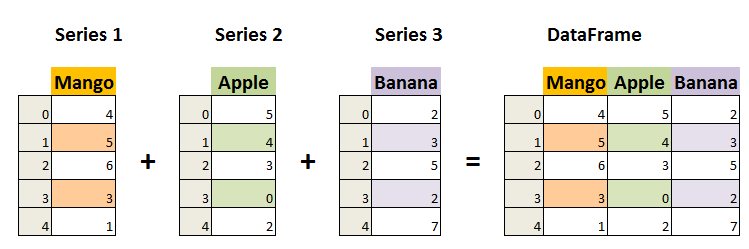
\includegraphics{images/df-dp.png}

\begin{Shaded}
\begin{Highlighting}[]
\CommentTok{\# 惯例导入2个模块}
\ImportTok{import}\NormalTok{ pandas }\ImportTok{as}\NormalTok{ pd}
\ImportTok{import}\NormalTok{ numpy }\ImportTok{as}\NormalTok{ np}

\CommentTok{\# 从字典创建,后面会详述}
\NormalTok{df }\OperatorTok{=}\NormalTok{ pd.DataFrame(}\BuiltInTok{dict}\NormalTok{(}\BuiltInTok{id}\OperatorTok{=}\NormalTok{[}\DecValTok{1}\NormalTok{,}\DecValTok{2}\NormalTok{,}\DecValTok{3}\NormalTok{],name }\OperatorTok{=}\NormalTok{ [}\StringTok{\textquotesingle{}a\textquotesingle{}}\NormalTok{,}\StringTok{\textquotesingle{}b\textquotesingle{}}\NormalTok{,}\StringTok{\textquotesingle{}c\textquotesingle{}}\NormalTok{]))}

\NormalTok{df}
\end{Highlighting}
\end{Shaded}

\begin{longtable}[]{@{}lll@{}}
\toprule\noalign{}
& id & name \\
\midrule\noalign{}
\endhead
\bottomrule\noalign{}
\endlastfoot
0 & 1 & a \\
1 & 2 & b \\
2 & 3 & c \\
\end{longtable}

\begin{Shaded}
\begin{Highlighting}[]
\CommentTok{\# 取某一列:得到一个Series,注意Series由index和value组成}
\NormalTok{x }\OperatorTok{=}\NormalTok{ df[}\StringTok{\textquotesingle{}name\textquotesingle{}}\NormalTok{]}
\BuiltInTok{print}\NormalTok{(x)}
\BuiltInTok{print}\NormalTok{(}\BuiltInTok{type}\NormalTok{(x))}
\end{Highlighting}
\end{Shaded}

\begin{verbatim}
0    a
1    b
2    c
Name: name, dtype: object
<class 'pandas.core.series.Series'>
\end{verbatim}

\begin{Shaded}
\begin{Highlighting}[]
\CommentTok{\# x的index}
\BuiltInTok{print}\NormalTok{(x.index)}
\BuiltInTok{print}\NormalTok{(}\BuiltInTok{type}\NormalTok{(x.index))}
\end{Highlighting}
\end{Shaded}

\begin{verbatim}
RangeIndex(start=0, stop=3, step=1)
<class 'pandas.core.indexes.range.RangeIndex'>
\end{verbatim}

\begin{Shaded}
\begin{Highlighting}[]
\CommentTok{\# x的value}
\BuiltInTok{print}\NormalTok{(x.values)}
\BuiltInTok{print}\NormalTok{(}\BuiltInTok{type}\NormalTok{(x.values)) }\CommentTok{\# 是一个ndarray}
\end{Highlighting}
\end{Shaded}

\begin{verbatim}
['a' 'b' 'c']
<class 'numpy.ndarray'>
\end{verbatim}

\hypertarget{dataframeux7684ux521bux5efa}{%
\section{DataFrame的创建}\label{dataframeux7684ux521bux5efa}}

\begin{Shaded}
\begin{Highlighting}[]
\CommentTok{\# 从ndarray或者list创建}

\NormalTok{a }\OperatorTok{=}\NormalTok{ np.array([}\DecValTok{8}\NormalTok{,}\DecValTok{6}\NormalTok{,}\DecValTok{4}\NormalTok{,}\DecValTok{2}\NormalTok{])}
\BuiltInTok{print}\NormalTok{(a)}

\NormalTok{df1 }\OperatorTok{=}\NormalTok{ pd.DataFrame(a)}
\NormalTok{df1}
\end{Highlighting}
\end{Shaded}

\begin{verbatim}
[8 6 4 2]
\end{verbatim}

\begin{longtable}[]{@{}ll@{}}
\toprule\noalign{}
& 0 \\
\midrule\noalign{}
\endhead
\bottomrule\noalign{}
\endlastfoot
0 & 8 \\
1 & 6 \\
2 & 4 \\
3 & 2 \\
\end{longtable}

\begin{Shaded}
\begin{Highlighting}[]
\NormalTok{b }\OperatorTok{=} \BuiltInTok{list}\NormalTok{(}\StringTok{\textquotesingle{}apple\textquotesingle{}}\NormalTok{)}
\BuiltInTok{print}\NormalTok{(b)}
\NormalTok{df2 }\OperatorTok{=}\NormalTok{ pd.DataFrame(b, columns}\OperatorTok{=}\NormalTok{[}\StringTok{\textquotesingle{}B\textquotesingle{}}\NormalTok{],index }\OperatorTok{=} \BuiltInTok{list}\NormalTok{(}\StringTok{\textquotesingle{}abcde\textquotesingle{}}\NormalTok{)) }\CommentTok{\# 指定columns和index}
\NormalTok{df2}
\end{Highlighting}
\end{Shaded}

\begin{verbatim}
['a', 'p', 'p', 'l', 'e']
\end{verbatim}

\begin{longtable}[]{@{}ll@{}}
\toprule\noalign{}
& B \\
\midrule\noalign{}
\endhead
\bottomrule\noalign{}
\endlastfoot
a & a \\
b & p \\
c & p \\
d & l \\
e & e \\
\end{longtable}

\begin{Shaded}
\begin{Highlighting}[]
\CommentTok{\# 从字典创建}

\CommentTok{\# 字典的每一个item会成为表格的一列,key会成为列标签(列的标题),value会成为列的值}
\NormalTok{x }\OperatorTok{=} \BuiltInTok{dict}\NormalTok{(A }\OperatorTok{=}\NormalTok{ [}\DecValTok{1}\NormalTok{,}\DecValTok{2}\NormalTok{,}\DecValTok{3}\NormalTok{,}\DecValTok{4}\NormalTok{,}\DecValTok{5}\NormalTok{], B }\OperatorTok{=} \BuiltInTok{list}\NormalTok{(}\StringTok{\textquotesingle{}APPLE\textquotesingle{}}\NormalTok{))}
\BuiltInTok{print}\NormalTok{(x)}
\NormalTok{df }\OperatorTok{=}\NormalTok{ pd.DataFrame(x)}
\NormalTok{df }
\end{Highlighting}
\end{Shaded}

\begin{verbatim}
{'A': [1, 2, 3, 4, 5], 'B': ['A', 'P', 'P', 'L', 'E']}
\end{verbatim}

\begin{longtable}[]{@{}lll@{}}
\toprule\noalign{}
& A & B \\
\midrule\noalign{}
\endhead
\bottomrule\noalign{}
\endlastfoot
0 & 1 & A \\
1 & 2 & P \\
2 & 3 & P \\
3 & 4 & L \\
4 & 5 & E \\
\end{longtable}

\begin{Shaded}
\begin{Highlighting}[]
\CommentTok{\# 单独设置或者修改列标签(columns)}
\BuiltInTok{print}\NormalTok{(df.columns)}
\NormalTok{df.columns }\OperatorTok{=}\NormalTok{ [}\StringTok{\textquotesingle{}C\textquotesingle{}}\NormalTok{,}\StringTok{\textquotesingle{}D\textquotesingle{}}\NormalTok{]}
\NormalTok{df}
\end{Highlighting}
\end{Shaded}

\begin{verbatim}
Index(['A', 'B'], dtype='object')
\end{verbatim}

\begin{longtable}[]{@{}lll@{}}
\toprule\noalign{}
& C & D \\
\midrule\noalign{}
\endhead
\bottomrule\noalign{}
\endlastfoot
0 & 1 & A \\
1 & 2 & P \\
2 & 3 & P \\
3 & 4 & L \\
4 & 5 & E \\
\end{longtable}

\begin{Shaded}
\begin{Highlighting}[]
\CommentTok{\# 单独修改行标签(index)}
\BuiltInTok{print}\NormalTok{(df.index)}
\NormalTok{df.index }\OperatorTok{=}\NormalTok{ [}\DecValTok{5}\NormalTok{,}\DecValTok{6}\NormalTok{,}\DecValTok{7}\NormalTok{,}\DecValTok{8}\NormalTok{,}\DecValTok{9}\NormalTok{]}
\NormalTok{df}
\end{Highlighting}
\end{Shaded}

\begin{verbatim}
RangeIndex(start=0, stop=5, step=1)
\end{verbatim}

\begin{longtable}[]{@{}lll@{}}
\toprule\noalign{}
& C & D \\
\midrule\noalign{}
\endhead
\bottomrule\noalign{}
\endlastfoot
5 & 1 & A \\
6 & 2 & P \\
7 & 3 & P \\
8 & 4 & L \\
9 & 5 & E \\
\end{longtable}

\hypertarget{ux6570ux636eux8bfbux53d6}{%
\section{数据读取}\label{ux6570ux636eux8bfbux53d6}}

\hypertarget{ux9884ux5907ux77e5ux8bc6ux5e38ux89c1ux6570ux636eux683cux5f0f}{%
\subsection{预备知识:常见数据格式}\label{ux9884ux5907ux77e5ux8bc6ux5e38ux89c1ux6570ux636eux683cux5f0f}}

一般常见的数据格式包括:

\begin{enumerate}
\def\labelenumi{\arabic{enumi}.}
\tightlist
\item
  微软的Excel格式:2007版以后扩展名为\texttt{.xlsx},2007版之前为\texttt{.xls},可以直接用Excel打开处理,不详细叙述。
\item
  CSV格式:扩展名为\texttt{.csv},也可以用Excel打开。但这种文件本质上是一个纯文本文件,和\texttt{.txt}文件或者python代码\texttt{.py}文件并无区别,都可以用记事本或者vscode打开。
\end{enumerate}

其中:

\begin{enumerate}
\def\labelenumi{\arabic{enumi}.}
\tightlist
\item
  CSV文件:其中所有的信息都是数据,不包括格式、排版、颜色等等,文件体积小,几乎任何数据处理软件都可以处理CSV文件。可以视为通用标准,你不知道要保存成什么格式,就可以用CSV。
\item
  Excel文件:文件里包括了大量的格式、排版、颜色等信息,文件体积比较大,多数数据处理软件都可以处理。如果你可以选择,就选择新版格式\texttt{.xlsx}。
\end{enumerate}

对于我们大部分工作,两种保存数据的格式都没有本质的区别。

以下数据如果不做说明,都来自CSMAR(国泰安)数据库。

vscode管理工程以目录为基础,很多功能需要你\textbf{打开一个目录}才能生效。你在vscode中打开的目录即\textbf{工作目录}。

在本课程中,所有的数据,都会放在工作目录下的\textbf{data}文件夹。即\texttt{data}文件夹现在这个\texttt{.ipynb}处于目录同一层。

所用数据包括:

\begin{enumerate}
\def\labelenumi{\arabic{enumi}.}
\tightlist
\item
  data/basic\_info.xlsx:部分上市公司的基本信息。
\end{enumerate}

\begin{Shaded}
\begin{Highlighting}[]
\CommentTok{\# 导入pandas和numpy是惯例}
\ImportTok{import}\NormalTok{ pandas }\ImportTok{as}\NormalTok{ pd}
\ImportTok{import}\NormalTok{ numpy }\ImportTok{as}\NormalTok{ np}

\CommentTok{\# 读取工作目录下的data文件夹下的basic\_info.xlsx文件}
\CommentTok{\# 保存到df变量}
\NormalTok{df }\OperatorTok{=}\NormalTok{ pd.read\_excel(}\StringTok{\textquotesingle{}data/basic\_info.xlsx\textquotesingle{}}\NormalTok{) }
\end{Highlighting}
\end{Shaded}

读取数据后,首先检查数据读取是否符合预期。

用\texttt{.head()}方法检查前几行,\texttt{.tail()}检查后几行,默认都是5行。

\begin{Shaded}
\begin{Highlighting}[]
\NormalTok{df.head() }\CommentTok{\# 查看df的前5行}
\end{Highlighting}
\end{Shaded}

\begin{longtable}[]{@{}lllllllll@{}}
\toprule\noalign{}
& 股票代码 & 股票简称 & 公司成立日期 & 注册资本 & 首次上市日期 &
所属省份 & 所属城市 & 上市状态 \\
\midrule\noalign{}
\endhead
\bottomrule\noalign{}
\endlastfoot
0 & 1 & 平安银行 & 1987-12-22 & 19405918198 & 1991-04-03 & 广东省 &
深圳市 & 正常上市 \\
1 & 2 & 万科A & 1988-11-01 & 11625383375 & 1991-01-29 & 广东省 & 深圳市
& 正常上市 \\
2 & 4 & 国华网安 & 1986-05-05 & 156003000 & 1991-01-14 & 广东省 & 深圳市
& ST \\
3 & 5 & ST 星源 & 1990-02-01 & 1058536842 & 1990-12-10 & 广东省 & 深圳市
& ST \\
4 & 6 & 深振业A & 1989-04-01 & 1349995046 & 1992-04-27 & 广东省 & 深圳市
& 正常上市 \\
\end{longtable}

再用\texttt{.info()}看每一列的信息,主要看格式。

\begin{Shaded}
\begin{Highlighting}[]
\NormalTok{df.info()  }\CommentTok{\# 每一列的信息}
\end{Highlighting}
\end{Shaded}

\begin{verbatim}
<class 'pandas.core.frame.DataFrame'>
RangeIndex: 39 entries, 0 to 38
Data columns (total 8 columns):
 #   Column  Non-Null Count  Dtype 
---  ------  --------------  ----- 
 0   股票代码    39 non-null     int64 
 1   股票简称    39 non-null     object
 2   公司成立日期  39 non-null     object
 3   注册资本    39 non-null     int64 
 4   首次上市日期  39 non-null     object
 5   所属省份    39 non-null     object
 6   所属城市    39 non-null     object
 7   上市状态    39 non-null     object
dtypes: int64(2), object(6)
memory usage: 2.6+ KB
\end{verbatim}

\hypertarget{ux6570ux636eux683cux5f0fux7684ux8f6cux6362}{%
\subsection{数据格式的转换}\label{ux6570ux636eux683cux5f0fux7684ux8f6cux6362}}

我们首先观察到:

\begin{enumerate}
\def\labelenumi{\arabic{enumi}.}
\tightlist
\item
  股票代码不对,如平安银行的代码应该是\texttt{000001}。
  读取时默认把\texttt{股票代码}列识别为数字\texttt{int64}(见\texttt{info()}的结果),
  因此前面的0就被去掉了。
\item
  日期不是日期格式:从\texttt{info()}结果看,数据类型\texttt{Dtype}中,字符串\texttt{str}会被显示为\texttt{object}。
  (更深入的解释见
  \url{https://stackoverflow.com/questions/21018654/strings-in-a-dataframe-but-dtype-is-object}
  )
\end{enumerate}

(为什么日期数据最好是日期格式?比如你可以比较日期的先后,两个日期相减获得相差几天等等,但你无法对字符串型的日期做这类操作。)

处理这类问题一般可以 1. 在读取数据的时候就指定格式。2.
读取了数据后再转换。

\begin{enumerate}
\def\labelenumi{\arabic{enumi}.}
\tightlist
\item
  读取时指定格式:
\end{enumerate}

\texttt{pd.read\_xxx()}方法,可以接收一个参数\texttt{converters},这个参数是一个字典,其中key为列名,value转换的函数。

这里我们指定\texttt{股票代码}为字符串\texttt{str},用\texttt{str}函数即可;公司成立日期为\texttt{datetime}格式,用\texttt{pd.to\_datetime}函数。(这里故意漏掉\texttt{首次上市日期})

注:这里只是告诉pandas可以用什么函数来转换指定的列,而不是你自己去调用某个函数,因此只要函数名即可。

\begin{Shaded}
\begin{Highlighting}[]
\NormalTok{df }\OperatorTok{=}\NormalTok{ pd.read\_excel(}\StringTok{\textquotesingle{}data/basic\_info.xlsx\textquotesingle{}}\NormalTok{,}
\NormalTok{                   converters}\OperatorTok{=}\NormalTok{\{}\StringTok{\textquotesingle{}股票代码\textquotesingle{}}\NormalTok{:}\BuiltInTok{str}\NormalTok{,}\StringTok{\textquotesingle{}公司成立日期\textquotesingle{}}\NormalTok{:pd.to\_datetime\})}

\NormalTok{df.head()}
\end{Highlighting}
\end{Shaded}

\begin{longtable}[]{@{}lllllllll@{}}
\toprule\noalign{}
& 股票代码 & 股票简称 & 公司成立日期 & 注册资本 & 首次上市日期 &
所属省份 & 所属城市 & 上市状态 \\
\midrule\noalign{}
\endhead
\bottomrule\noalign{}
\endlastfoot
0 & 000001 & 平安银行 & 1987-12-22 & 19405918198 & 1991-04-03 & 广东省 &
深圳市 & 正常上市 \\
1 & 000002 & 万科A & 1988-11-01 & 11625383375 & 1991-01-29 & 广东省 &
深圳市 & 正常上市 \\
2 & 000004 & 国华网安 & 1986-05-05 & 156003000 & 1991-01-14 & 广东省 &
深圳市 & ST \\
3 & 000005 & ST 星源 & 1990-02-01 & 1058536842 & 1990-12-10 & 广东省 &
深圳市 & ST \\
4 & 000006 & 深振业A & 1989-04-01 & 1349995046 & 1992-04-27 & 广东省 &
深圳市 & 正常上市 \\
\end{longtable}

\begin{Shaded}
\begin{Highlighting}[]
\NormalTok{df.info()}
\end{Highlighting}
\end{Shaded}

\begin{verbatim}
<class 'pandas.core.frame.DataFrame'>
RangeIndex: 39 entries, 0 to 38
Data columns (total 8 columns):
 #   Column  Non-Null Count  Dtype         
---  ------  --------------  -----         
 0   股票代码    39 non-null     object        
 1   股票简称    39 non-null     object        
 2   公司成立日期  39 non-null     datetime64[ns]
 3   注册资本    39 non-null     int64         
 4   首次上市日期  39 non-null     object        
 5   所属省份    39 non-null     object        
 6   所属城市    39 non-null     object        
 7   上市状态    39 non-null     object        
dtypes: datetime64[ns](1), int64(1), object(6)
memory usage: 2.6+ KB
\end{verbatim}

查看数据的前几行以及列信息,股票代码和公司成立日期都符合我们的要求了。

\begin{enumerate}
\def\labelenumi{\arabic{enumi}.}
\setcounter{enumi}{1}
\tightlist
\item
  读取后再转换
\end{enumerate}

读取\texttt{首次上市日期}列,转换格式,再写回到同一列中。对行和列的读写是后面的内容,但逻辑还是比较简单。

\begin{Shaded}
\begin{Highlighting}[]
\NormalTok{df[}\StringTok{\textquotesingle{}首次上市日期\textquotesingle{}}\NormalTok{] }\OperatorTok{=}\NormalTok{ pd.to\_datetime(df[}\StringTok{\textquotesingle{}首次上市日期\textquotesingle{}}\NormalTok{])}
\NormalTok{df.info()}
\end{Highlighting}
\end{Shaded}

\begin{verbatim}
<class 'pandas.core.frame.DataFrame'>
RangeIndex: 39 entries, 0 to 38
Data columns (total 8 columns):
 #   Column  Non-Null Count  Dtype         
---  ------  --------------  -----         
 0   股票代码    39 non-null     object        
 1   股票简称    39 non-null     object        
 2   公司成立日期  39 non-null     datetime64[ns]
 3   注册资本    39 non-null     int64         
 4   首次上市日期  39 non-null     datetime64[ns]
 5   所属省份    39 non-null     object        
 6   所属城市    39 non-null     object        
 7   上市状态    39 non-null     object        
dtypes: datetime64[ns](2), int64(1), object(5)
memory usage: 2.6+ KB
\end{verbatim}

查看\texttt{info()},数据已经符合我们的要求。

\hypertarget{dataframeux7684ux7d22ux5f15ux548cux884cux5217ux6807ux7b7e}{%
\section{DataFrame的索引和行列标签}\label{dataframeux7684ux7d22ux5f15ux548cux884cux5217ux6807ux7b7e}}

\begin{Shaded}
\begin{Highlighting}[]
\NormalTok{df.head()}
\end{Highlighting}
\end{Shaded}

\begin{longtable}[]{@{}lllllllll@{}}
\toprule\noalign{}
& 股票代码 & 股票简称 & 公司成立日期 & 注册资本 & 首次上市日期 &
所属省份 & 所属城市 & 上市状态 \\
\midrule\noalign{}
\endhead
\bottomrule\noalign{}
\endlastfoot
0 & 000001 & 平安银行 & 1987-12-22 & 19405918198 & 1991-04-03 & 广东省 &
深圳市 & 正常上市 \\
1 & 000002 & 万科A & 1988-11-01 & 11625383375 & 1991-01-29 & 广东省 &
深圳市 & 正常上市 \\
2 & 000004 & 国华网安 & 1986-05-05 & 156003000 & 1991-01-14 & 广东省 &
深圳市 & ST \\
3 & 000005 & ST 星源 & 1990-02-01 & 1058536842 & 1990-12-10 & 广东省 &
深圳市 & ST \\
4 & 000006 & 深振业A & 1989-04-01 & 1349995046 & 1992-04-27 & 广东省 &
深圳市 & 正常上市 \\
\end{longtable}

对于一个DataFrame对象,每一列的标题(题头)和每一行的索引,其实都是索引index,或可称为行索引和列索引。

获得所有的列名(即获得所有的列索引):这是一个字符串类型的索引,包括每一列的列名。

\begin{Shaded}
\begin{Highlighting}[]
\NormalTok{df.columns}
\end{Highlighting}
\end{Shaded}

\begin{verbatim}
Index(['股票代码', '股票简称', '公司成立日期', '注册资本', '首次上市日期', '所属省份', '所属城市', '上市状态'], dtype='object')
\end{verbatim}

获得所有的行索引:这是一个range类的索引,从0到39。如果是时间序列数据,还可以是日期格式的行索引。

\begin{Shaded}
\begin{Highlighting}[]
\NormalTok{df.index}
\end{Highlighting}
\end{Shaded}

\begin{verbatim}
RangeIndex(start=0, stop=39, step=1)
\end{verbatim}

我们可以用\texttt{set\_index()}指定一列作为行索引,比如股票代码。

\begin{Shaded}
\begin{Highlighting}[]
\NormalTok{df }\OperatorTok{=}\NormalTok{ df.set\_index(}\StringTok{\textquotesingle{}股票代码\textquotesingle{}}\NormalTok{) }
\NormalTok{df.head()}
\end{Highlighting}
\end{Shaded}

\begin{longtable}[]{@{}llllllll@{}}
\toprule\noalign{}
& 股票简称 & 公司成立日期 & 注册资本 & 首次上市日期 & 所属省份 &
所属城市 & 上市状态 \\
股票代码 & & & & & & & \\
\midrule\noalign{}
\endhead
\bottomrule\noalign{}
\endlastfoot
000001 & 平安银行 & 1987-12-22 & 19405918198 & 1991-04-03 & 广东省 &
深圳市 & 正常上市 \\
000002 & 万科A & 1988-11-01 & 11625383375 & 1991-01-29 & 广东省 & 深圳市
& 正常上市 \\
000004 & 国华网安 & 1986-05-05 & 156003000 & 1991-01-14 & 广东省 &
深圳市 & ST \\
000005 & ST 星源 & 1990-02-01 & 1058536842 & 1990-12-10 & 广东省 &
深圳市 & ST \\
000006 & 深振业A & 1989-04-01 & 1349995046 & 1992-04-27 & 广东省 &
深圳市 & 正常上市 \\
\end{longtable}

注意:pandas中,大部分``写''操作(修改某个东西),默认都``不会改变原值'':你会获得一个包括修改后的新数据的DataFrame。
因此,如果要改变原值,可以把新数据重新赋值给原来的变量名(如上个cell),也可以加入参数\texttt{inplace\ =\ True},如

\begin{Shaded}
\begin{Highlighting}[]
\CommentTok{\# 仅作示范,不要执行,因为经过上个cell之后,已经没有\textasciigrave{}股票代码\textasciigrave{}这一列了}
\CommentTok{\# df.set\_index(\textquotesingle{}股票代码\textquotesingle{},inplace = True)}
\end{Highlighting}
\end{Shaded}

再看\texttt{df.index},此时索引已经变成我们指定列,

\begin{Shaded}
\begin{Highlighting}[]
\NormalTok{df.index}
\end{Highlighting}
\end{Shaded}

\begin{verbatim}
Index(['000001', '000002', '000004', '000005', '000006', '000007', '000008',
       '000009', '000010', '000011', '000012', '000014', '000016', '000017',
       '000019', '000020', '000021', '000023', '000025', '000026', '000027',
       '000028', '000029', '000030', '000031', '000032', '000034', '000035',
       '000036', '000037', '000038', '000039', '000040', '000042', '000045',
       '000046', '000048', '000049', '000050'],
      dtype='object', name='股票代码')
\end{verbatim}

重命名列标签是可以常用操作(改列名),一般有两种方式:

\begin{enumerate}
\def\labelenumi{\arabic{enumi}.}
\tightlist
\item
  使用\texttt{.rename()}方法:这个方法接受一个字典参数\texttt{columns},其中key是旧名,value是新名。(从旧到新的映射)
\item
  对\texttt{df.columns} 整体重新赋值。注意,这个方法会直接修改原数据。
\end{enumerate}

例如:把``首次上市日期''改为``IPO\_DATE'':

\begin{Shaded}
\begin{Highlighting}[]
\CommentTok{\# 方法1:rename()}

\NormalTok{df.rename(columns}\OperatorTok{=}\NormalTok{\{}\StringTok{\textquotesingle{}首次上市日期\textquotesingle{}}\NormalTok{:}\StringTok{\textquotesingle{}IPO\_DATE\textquotesingle{}}\NormalTok{\}).head()}
\CommentTok{\# 这里不使用inplace = True,因此会返回一个新的数据,不会改写原数据。}
\end{Highlighting}
\end{Shaded}

\begin{longtable}[]{@{}llllllll@{}}
\toprule\noalign{}
& 股票简称 & 公司成立日期 & 注册资本 & IPO\_DATE & 所属省份 & 所属城市 &
上市状态 \\
股票代码 & & & & & & & \\
\midrule\noalign{}
\endhead
\bottomrule\noalign{}
\endlastfoot
000001 & 平安银行 & 1987-12-22 & 19405918198 & 1991-04-03 & 广东省 &
深圳市 & 正常上市 \\
000002 & 万科A & 1988-11-01 & 11625383375 & 1991-01-29 & 广东省 & 深圳市
& 正常上市 \\
000004 & 国华网安 & 1986-05-05 & 156003000 & 1991-01-14 & 广东省 &
深圳市 & ST \\
000005 & ST 星源 & 1990-02-01 & 1058536842 & 1990-12-10 & 广东省 &
深圳市 & ST \\
000006 & 深振业A & 1989-04-01 & 1349995046 & 1992-04-27 & 广东省 &
深圳市 & 正常上市 \\
\end{longtable}

\begin{Shaded}
\begin{Highlighting}[]
\CommentTok{\# 方法2:对columns重新赋值}

\NormalTok{df2 }\OperatorTok{=}\NormalTok{ df.copy() }\CommentTok{\# 这个方法会直接修改原值。为了保持原数据不变,在一个副本上演示。}

\NormalTok{df2.columns }\OperatorTok{=} \BuiltInTok{list}\NormalTok{(}\StringTok{\textquotesingle{}ABCDEFG\textquotesingle{}}\NormalTok{) }\CommentTok{\# 赋值一个同样长度的list。}
\NormalTok{df2.head() }\CommentTok{\# df2的列名直接被改变了。}
\end{Highlighting}
\end{Shaded}

\begin{longtable}[]{@{}llllllll@{}}
\toprule\noalign{}
& A & B & C & D & E & F & G \\
股票代码 & & & & & & & \\
\midrule\noalign{}
\endhead
\bottomrule\noalign{}
\endlastfoot
000001 & 平安银行 & 1987-12-22 & 19405918198 & 1991-04-03 & 广东省 &
深圳市 & 正常上市 \\
000002 & 万科A & 1988-11-01 & 11625383375 & 1991-01-29 & 广东省 & 深圳市
& 正常上市 \\
000004 & 国华网安 & 1986-05-05 & 156003000 & 1991-01-14 & 广东省 &
深圳市 & ST \\
000005 & ST 星源 & 1990-02-01 & 1058536842 & 1990-12-10 & 广东省 &
深圳市 & ST \\
000006 & 深振业A & 1989-04-01 & 1349995046 & 1992-04-27 & 广东省 &
深圳市 & 正常上市 \\
\end{longtable}

\hypertarget{ux5728ux884cux4e0eux5217ux4e0aux5de5ux4f5c}{%
\section{在行与列上工作}\label{ux5728ux884cux4e0eux5217ux4e0aux5de5ux4f5c}}

选择行和列的一万种方法。

\hypertarget{ux9009ux62e9ux5217}{%
\subsection{选择列}\label{ux9009ux62e9ux5217}}

选1列,\texttt{{[}列名{]}},返回一个\texttt{Series}对象。

\begin{Shaded}
\begin{Highlighting}[]
\NormalTok{sec\_name }\OperatorTok{=}\NormalTok{ df[}\StringTok{\textquotesingle{}股票简称\textquotesingle{}}\NormalTok{]}
\NormalTok{sec\_name.head()}
\end{Highlighting}
\end{Shaded}

\begin{verbatim}
股票代码
000001     平安银行
000002      万科A
000004     国华网安
000005    ST 星源
000006     深振业A
Name: 股票简称, dtype: object
\end{verbatim}

查看列的类型

\begin{Shaded}
\begin{Highlighting}[]
\BuiltInTok{type}\NormalTok{(sec\_name) }\CommentTok{\# pandas.core.series.Series }
\end{Highlighting}
\end{Shaded}

\begin{verbatim}
pandas.core.series.Series
\end{verbatim}

选择多列,\texttt{{[}{[}列名的List{]}{]}},返回一个\texttt{DataFrame}对象。

\begin{Shaded}
\begin{Highlighting}[]
\NormalTok{df[[}\StringTok{\textquotesingle{}股票简称\textquotesingle{}}\NormalTok{,}\StringTok{\textquotesingle{}上市状态\textquotesingle{}}\NormalTok{]].head()}
\end{Highlighting}
\end{Shaded}

\begin{longtable}[]{@{}lll@{}}
\toprule\noalign{}
& 股票简称 & 上市状态 \\
股票代码 & & \\
\midrule\noalign{}
\endhead
\bottomrule\noalign{}
\endlastfoot
000001 & 平安银行 & 正常上市 \\
000002 & 万科A & 正常上市 \\
000004 & 国华网安 & ST \\
000005 & ST 星源 & ST \\
000006 & 深振业A & 正常上市 \\
\end{longtable}

\hypertarget{locux6309ux7d22ux5f15ux53d6ux5f97ux884cux548cux5217}{%
\subsection{loc:按索引取得行和列}\label{locux6309ux7d22ux5f15ux53d6ux5f97ux884cux548cux5217}}

\texttt{.loc{[}行索引,列索引{]}}可以按\textbf{索引}选择行或者列(行的索引是index,列的索引是columns)

\begin{Shaded}
\begin{Highlighting}[]
\NormalTok{df.loc[[}\StringTok{\textquotesingle{}000001\textquotesingle{}}\NormalTok{,}\StringTok{\textquotesingle{}000002\textquotesingle{}}\NormalTok{],[}\StringTok{\textquotesingle{}股票简称\textquotesingle{}}\NormalTok{,}\StringTok{\textquotesingle{}上市状态\textquotesingle{}}\NormalTok{]]}
\end{Highlighting}
\end{Shaded}

\begin{longtable}[]{@{}lll@{}}
\toprule\noalign{}
& 股票简称 & 上市状态 \\
股票代码 & & \\
\midrule\noalign{}
\endhead
\bottomrule\noalign{}
\endlastfoot
000001 & 平安银行 & 正常上市 \\
000002 & 万科A & 正常上市 \\
\end{longtable}

也可以只取一个值:

\begin{Shaded}
\begin{Highlighting}[]
\NormalTok{df.loc[}\StringTok{\textquotesingle{}000001\textquotesingle{}}\NormalTok{,}\StringTok{\textquotesingle{}股票简称\textquotesingle{}}\NormalTok{]}
\end{Highlighting}
\end{Shaded}

\begin{verbatim}
'平安银行'
\end{verbatim}

行索引和列索引位置,都可以用冒号\texttt{:}表示起点和终点(注:起点终点都包括,和Python的List切片不同!)。

如果只有\texttt{:},则代表所有行或者列。

比如:获取行索引为\texttt{000001}到\texttt{000005},列索引为\texttt{股票简称}到\texttt{注册资本}之间的所有数据。

\begin{Shaded}
\begin{Highlighting}[]
\NormalTok{df.loc[}\StringTok{\textquotesingle{}000001\textquotesingle{}}\NormalTok{:}\StringTok{\textquotesingle{}000005\textquotesingle{}}\NormalTok{,}\StringTok{\textquotesingle{}股票简称\textquotesingle{}}\NormalTok{:}\StringTok{\textquotesingle{}注册资本\textquotesingle{}}\NormalTok{]}
\end{Highlighting}
\end{Shaded}

\begin{longtable}[]{@{}llll@{}}
\toprule\noalign{}
& 股票简称 & 公司成立日期 & 注册资本 \\
股票代码 & & & \\
\midrule\noalign{}
\endhead
\bottomrule\noalign{}
\endlastfoot
000001 & 平安银行 & 1987-12-22 & 19405918198 \\
000002 & 万科A & 1988-11-01 & 11625383375 \\
000004 & 国华网安 & 1986-05-05 & 156003000 \\
000005 & ST 星源 & 1990-02-01 & 1058536842 \\
\end{longtable}

获取``所有行(所有股票)的股票简称和上市状况''。但太长,只查看前几行

\begin{Shaded}
\begin{Highlighting}[]
\NormalTok{x }\OperatorTok{=}\NormalTok{ df.loc[ : ,[}\StringTok{\textquotesingle{}股票简称\textquotesingle{}}\NormalTok{,}\StringTok{\textquotesingle{}上市状态\textquotesingle{}}\NormalTok{]]}
\NormalTok{x.head()}
\end{Highlighting}
\end{Shaded}

\begin{longtable}[]{@{}lll@{}}
\toprule\noalign{}
& 股票简称 & 上市状态 \\
股票代码 & & \\
\midrule\noalign{}
\endhead
\bottomrule\noalign{}
\endlastfoot
000001 & 平安银行 & 正常上市 \\
000002 & 万科A & 正常上市 \\
000004 & 国华网安 & ST \\
000005 & ST 星源 & ST \\
000006 & 深振业A & 正常上市 \\
\end{longtable}

当然,如果只是取某列的全部行,上面的代码就和\texttt{df{[}{[}\textquotesingle{}股票简称\textquotesingle{},\textquotesingle{}上市状态\textquotesingle{}{]}{]}}等价。

同Python的切片,冒号一侧不写,则表示``到尽头''。

\begin{Shaded}
\begin{Highlighting}[]
\NormalTok{x }\OperatorTok{=}\NormalTok{ df.loc[:}\StringTok{\textquotesingle{}000002\textquotesingle{}}\NormalTok{,}\StringTok{\textquotesingle{}所属城市\textquotesingle{}}\NormalTok{:]}
\NormalTok{x}
\end{Highlighting}
\end{Shaded}

\begin{longtable}[]{@{}lll@{}}
\toprule\noalign{}
& 所属城市 & 上市状态 \\
股票代码 & & \\
\midrule\noalign{}
\endhead
\bottomrule\noalign{}
\endlastfoot
000001 & 深圳市 & 正常上市 \\
000002 & 深圳市 & 正常上市 \\
\end{longtable}

\hypertarget{ux5217ux7684ux6b21ux5e8f}{%
\subsection{列的次序}\label{ux5217ux7684ux6b21ux5e8f}}

在选择列的操作中,列的次序和你提供的列名List的次序完全一样。因此,取列的操作,包括\texttt{{[}{]}}和\texttt{.loc{[}{]}},都可以用于改变列的次序。

例如,把列名逆序:(当然,只要你获得了列名的List,就可以任意排序)

\begin{Shaded}
\begin{Highlighting}[]
\CommentTok{\# 逆序列名}
\NormalTok{cols }\OperatorTok{=}\NormalTok{ df.columns }\CommentTok{\# 取得列名}
\NormalTok{df[cols[::}\OperatorTok{{-}}\DecValTok{1}\NormalTok{]].head() }\CommentTok{\# 对逆序后的列名,用\textasciigrave{}[]\textasciigrave{}取列。当然,用df.loc[:,cols[::{-}1]]也一样。}
\end{Highlighting}
\end{Shaded}

\begin{longtable}[]{@{}llllllll@{}}
\toprule\noalign{}
& 上市状态 & 所属城市 & 所属省份 & 首次上市日期 & 注册资本 &
公司成立日期 & 股票简称 \\
股票代码 & & & & & & & \\
\midrule\noalign{}
\endhead
\bottomrule\noalign{}
\endlastfoot
000001 & 正常上市 & 深圳市 & 广东省 & 1991-04-03 & 19405918198 &
1987-12-22 & 平安银行 \\
000002 & 正常上市 & 深圳市 & 广东省 & 1991-01-29 & 11625383375 &
1988-11-01 & 万科A \\
000004 & ST & 深圳市 & 广东省 & 1991-01-14 & 156003000 & 1986-05-05 &
国华网安 \\
000005 & ST & 深圳市 & 广东省 & 1990-12-10 & 1058536842 & 1990-02-01 &
ST 星源 \\
000006 & 正常上市 & 深圳市 & 广东省 & 1992-04-27 & 1349995046 &
1989-04-01 & 深振业A \\
\end{longtable}

\hypertarget{ux5217ux8fd0ux7b97}{%
\subsection{列运算}\label{ux5217ux8fd0ux7b97}}

每一列之间可以很方便地进行运算:任何操作都会自动应用到每一列的所有元素(如同NumPy中的广播)

例如,注册资本转换为亿元,并保留2位数字。

\begin{Shaded}
\begin{Highlighting}[]
\NormalTok{(df[}\StringTok{\textquotesingle{}注册资本\textquotesingle{}}\NormalTok{] }\OperatorTok{/} \DecValTok{100000000}\NormalTok{).}\BuiltInTok{round}\NormalTok{(}\DecValTok{2}\NormalTok{).head()}
\end{Highlighting}
\end{Shaded}

\begin{verbatim}
股票代码
000001    194.06
000002    116.25
000004      1.56
000005     10.59
000006     13.50
Name: 注册资本, dtype: float64
\end{verbatim}

注意到,Series经过运算后也会得到一个Series,可以加入原数据中的一个列:直接=赋值即可。

\begin{Shaded}
\begin{Highlighting}[]
\NormalTok{df[}\StringTok{\textquotesingle{}注册资本\_亿\textquotesingle{}}\NormalTok{] }\OperatorTok{=}\NormalTok{ (df[}\StringTok{\textquotesingle{}注册资本\textquotesingle{}}\NormalTok{] }\OperatorTok{/} \DecValTok{100000000}\NormalTok{).}\BuiltInTok{round}\NormalTok{(}\DecValTok{2}\NormalTok{)}
\NormalTok{df.head()}
\end{Highlighting}
\end{Shaded}

\begin{longtable}[]{@{}lllllllll@{}}
\toprule\noalign{}
& 股票简称 & 公司成立日期 & 注册资本 & 首次上市日期 & 所属省份 &
所属城市 & 上市状态 & 注册资本\_亿 \\
股票代码 & & & & & & & & \\
\midrule\noalign{}
\endhead
\bottomrule\noalign{}
\endlastfoot
000001 & 平安银行 & 1987-12-22 & 19405918198 & 1991-04-03 & 广东省 &
深圳市 & 正常上市 & 194.06 \\
000002 & 万科A & 1988-11-01 & 11625383375 & 1991-01-29 & 广东省 & 深圳市
& 正常上市 & 116.25 \\
000004 & 国华网安 & 1986-05-05 & 156003000 & 1991-01-14 & 广东省 &
深圳市 & ST & 1.56 \\
000005 & ST 星源 & 1990-02-01 & 1058536842 & 1990-12-10 & 广东省 &
深圳市 & ST & 10.59 \\
000006 & 深振业A & 1989-04-01 & 1349995046 & 1992-04-27 & 广东省 &
深圳市 & 正常上市 & 13.50 \\
\end{longtable}

\hypertarget{ux5220ux9664ux884cux6216ux8005ux5217}{%
\subsection{删除行或者列}\label{ux5220ux9664ux884cux6216ux8005ux5217}}

使用\texttt{df.drop(行或者列标签,axis=0\textbar{}1)}删除行或者列,其中参数axis
= 0为行,=1为列。

\begin{Shaded}
\begin{Highlighting}[]
\CommentTok{\# 删除“注册资本”列;如果要修改df本身,则inplace = True}
\NormalTok{df.drop(}\StringTok{\textquotesingle{}注册资本\textquotesingle{}}\NormalTok{,axis }\OperatorTok{=} \DecValTok{1}\NormalTok{).head()}
\end{Highlighting}
\end{Shaded}

\begin{longtable}[]{@{}llllllll@{}}
\toprule\noalign{}
& 股票简称 & 公司成立日期 & 首次上市日期 & 所属省份 & 所属城市 &
上市状态 & 注册资本\_亿 \\
股票代码 & & & & & & & \\
\midrule\noalign{}
\endhead
\bottomrule\noalign{}
\endlastfoot
000001 & 平安银行 & 1987-12-22 & 1991-04-03 & 广东省 & 深圳市 & 正常上市
& 194.06 \\
000002 & 万科A & 1988-11-01 & 1991-01-29 & 广东省 & 深圳市 & 正常上市 &
116.25 \\
000004 & 国华网安 & 1986-05-05 & 1991-01-14 & 广东省 & 深圳市 & ST &
1.56 \\
000005 & ST 星源 & 1990-02-01 & 1990-12-10 & 广东省 & 深圳市 & ST &
10.59 \\
000006 & 深振业A & 1989-04-01 & 1992-04-27 & 广东省 & 深圳市 & 正常上市
& 13.50 \\
\end{longtable}

\begin{Shaded}
\begin{Highlighting}[]
\CommentTok{\# 删除标签为00001的行}
\NormalTok{df.drop(}\StringTok{\textquotesingle{}000001\textquotesingle{}}\NormalTok{,axis}\OperatorTok{=}\DecValTok{0}\NormalTok{).head()}
\end{Highlighting}
\end{Shaded}

\begin{longtable}[]{@{}lllllllll@{}}
\toprule\noalign{}
& 股票简称 & 公司成立日期 & 注册资本 & 首次上市日期 & 所属省份 &
所属城市 & 上市状态 & 注册资本\_亿 \\
股票代码 & & & & & & & & \\
\midrule\noalign{}
\endhead
\bottomrule\noalign{}
\endlastfoot
000002 & 万科A & 1988-11-01 & 11625383375 & 1991-01-29 & 广东省 & 深圳市
& 正常上市 & 116.25 \\
000004 & 国华网安 & 1986-05-05 & 156003000 & 1991-01-14 & 广东省 &
深圳市 & ST & 1.56 \\
000005 & ST 星源 & 1990-02-01 & 1058536842 & 1990-12-10 & 广东省 &
深圳市 & ST & 10.59 \\
000006 & 深振业A & 1989-04-01 & 1349995046 & 1992-04-27 & 广东省 &
深圳市 & 正常上市 & 13.50 \\
000007 & *ST 全新 & 1988-11-21 & 346448044 & 1992-04-13 & 广东省 &
深圳市 & 正常上市 & 3.46 \\
\end{longtable}

注意:
pandas中,包括drop在内,很多操作``默认不修改原数据'',而是``修改后的数据作为返回值''。因此,需要这样把修改后的数据再次赋值。

\begin{Shaded}
\begin{Highlighting}[]
\NormalTok{df = df.drop( \textless{}参数\textgreater{} ) \# 把修改后的数据再次赋值给df}
\end{Highlighting}
\end{Shaded}

如果要``原地修改'',直接改变原始数据,那么需要添加
\texttt{inplace=True},此时原值被修改,返回值变为None。

\begin{Shaded}
\begin{Highlighting}[]
\NormalTok{df.drop( \textless{}参数\textgreater{}, inplace=True ) \# 在原始数据上修改,不用再赋值}
\end{Highlighting}
\end{Shaded}

\hypertarget{ilocux6309ux4f4dux7f6eux53d6ux5f97ux884cux548cux5217}{%
\subsection{iloc:按位置取得行和列}\label{ilocux6309ux4f4dux7f6eux53d6ux5f97ux884cux548cux5217}}

\texttt{.iloc{[}行坐标,列坐标{]}}:用法和\texttt{loc}非常类似,但只是把索引index(索引可以是任何序列),换成下标(从0开始)。

用法和Python的切片很类似。

\begin{Shaded}
\begin{Highlighting}[]
\CommentTok{\# 首先把股票代码还原成普通的列}
\NormalTok{df.reset\_index(inplace}\OperatorTok{=}\VariableTok{True}\NormalTok{)}
\NormalTok{df.head()}
\end{Highlighting}
\end{Shaded}

\begin{longtable}[]{@{}llllllllll@{}}
\toprule\noalign{}
& 股票代码 & 股票简称 & 公司成立日期 & 注册资本 & 首次上市日期 &
所属省份 & 所属城市 & 上市状态 & 注册资本\_亿 \\
\midrule\noalign{}
\endhead
\bottomrule\noalign{}
\endlastfoot
0 & 000001 & 平安银行 & 1987-12-22 & 19405918198 & 1991-04-03 & 广东省 &
深圳市 & 正常上市 & 194.06 \\
1 & 000002 & 万科A & 1988-11-01 & 11625383375 & 1991-01-29 & 广东省 &
深圳市 & 正常上市 & 116.25 \\
2 & 000004 & 国华网安 & 1986-05-05 & 156003000 & 1991-01-14 & 广东省 &
深圳市 & ST & 1.56 \\
3 & 000005 & ST 星源 & 1990-02-01 & 1058536842 & 1990-12-10 & 广东省 &
深圳市 & ST & 10.59 \\
4 & 000006 & 深振业A & 1989-04-01 & 1349995046 & 1992-04-27 & 广东省 &
深圳市 & 正常上市 & 13.50 \\
\end{longtable}

\begin{Shaded}
\begin{Highlighting}[]
\CommentTok{\# 取前5行,近似于df.head()}
\NormalTok{df.iloc[:}\DecValTok{5}\NormalTok{]}
\end{Highlighting}
\end{Shaded}

\begin{longtable}[]{@{}llllllllll@{}}
\toprule\noalign{}
& 股票代码 & 股票简称 & 公司成立日期 & 注册资本 & 首次上市日期 &
所属省份 & 所属城市 & 上市状态 & 注册资本\_亿 \\
\midrule\noalign{}
\endhead
\bottomrule\noalign{}
\endlastfoot
0 & 000001 & 平安银行 & 1987-12-22 & 19405918198 & 1991-04-03 & 广东省 &
深圳市 & 正常上市 & 194.06 \\
1 & 000002 & 万科A & 1988-11-01 & 11625383375 & 1991-01-29 & 广东省 &
深圳市 & 正常上市 & 116.25 \\
2 & 000004 & 国华网安 & 1986-05-05 & 156003000 & 1991-01-14 & 广东省 &
深圳市 & ST & 1.56 \\
3 & 000005 & ST 星源 & 1990-02-01 & 1058536842 & 1990-12-10 & 广东省 &
深圳市 & ST & 10.59 \\
4 & 000006 & 深振业A & 1989-04-01 & 1349995046 & 1992-04-27 & 广东省 &
深圳市 & 正常上市 & 13.50 \\
\end{longtable}

\begin{Shaded}
\begin{Highlighting}[]
\CommentTok{\# iloc接受列表,如取0,2,4,6行}
\NormalTok{df.iloc[[}\DecValTok{0}\NormalTok{,}\DecValTok{2}\NormalTok{,}\DecValTok{4}\NormalTok{,}\DecValTok{6}\NormalTok{]]}
\end{Highlighting}
\end{Shaded}

\begin{longtable}[]{@{}llllllllll@{}}
\toprule\noalign{}
& 股票代码 & 股票简称 & 公司成立日期 & 注册资本 & 首次上市日期 &
所属省份 & 所属城市 & 上市状态 & 注册资本\_亿 \\
\midrule\noalign{}
\endhead
\bottomrule\noalign{}
\endlastfoot
0 & 000001 & 平安银行 & 1987-12-22 & 19405918198 & 1991-04-03 & 广东省 &
深圳市 & 正常上市 & 194.06 \\
2 & 000004 & 国华网安 & 1986-05-05 & 156003000 & 1991-01-14 & 广东省 &
深圳市 & ST & 1.56 \\
4 & 000006 & 深振业A & 1989-04-01 & 1349995046 & 1992-04-27 & 广东省 &
深圳市 & 正常上市 & 13.50 \\
6 & 000008 & 神州高铁 & 1989-10-11 & 2780795346 & 1992-05-07 & 北京市 &
北京市 & 正常上市 & 27.81 \\
\end{longtable}

\begin{Shaded}
\begin{Highlighting}[]
\CommentTok{\# 抽样:随机选行。}
\NormalTok{df.sample(}\DecValTok{5}\NormalTok{)}
\end{Highlighting}
\end{Shaded}

\begin{longtable}[]{@{}llllllllll@{}}
\toprule\noalign{}
& 股票代码 & 股票简称 & 公司成立日期 & 注册资本 & 首次上市日期 &
所属省份 & 所属城市 & 上市状态 & 注册资本\_亿 \\
\midrule\noalign{}
\endhead
\bottomrule\noalign{}
\endlastfoot
28 & 000036 & 华联控股 & 1994-01-29 & 1483934025 & 1994-06-17 & 广东省 &
深圳市 & 正常上市 & 14.84 \\
13 & 000017 & 深中华A & 1992-03-12 & 551347947 & 1992-03-31 & 广东省 &
深圳市 & 正常上市 & 5.51 \\
7 & 000009 & 中国宝安 & 1990-09-01 & 2579213965 & 1991-06-25 & 广东省 &
深圳市 & 正常上市 & 25.79 \\
5 & 000007 & *ST 全新 & 1988-11-21 & 346448044 & 1992-04-13 & 广东省 &
深圳市 & 正常上市 & 3.46 \\
37 & 000049 & 德赛电池 & 1995-02-18 & 300298970 & 1995-03-20 & 广东省 &
深圳市 & 正常上市 & 3.00 \\
\end{longtable}

\hypertarget{ux6309ux6761ux4ef6ux7b5bux9009}{%
\subsection{按条件筛选}\label{ux6309ux6761ux4ef6ux7b5bux9009}}

\begin{Shaded}
\begin{Highlighting}[]
\CommentTok{\# 按条件筛选:如,选择注册资本大于20亿的公司}

\CommentTok{\# 创建条件}
\NormalTok{mask }\OperatorTok{=}\NormalTok{ df[}\StringTok{\textquotesingle{}注册资本\textquotesingle{}}\NormalTok{] }\OperatorTok{\textgreater{}} \DecValTok{2000000000}
\NormalTok{mask.head()}
\end{Highlighting}
\end{Shaded}

\begin{verbatim}
0     True
1     True
2    False
3    False
4    False
Name: 注册资本, dtype: bool
\end{verbatim}

\begin{Shaded}
\begin{Highlighting}[]
\NormalTok{df[mask]}
\end{Highlighting}
\end{Shaded}

\begin{longtable}[]{@{}llllllllll@{}}
\toprule\noalign{}
& 股票代码 & 股票简称 & 公司成立日期 & 注册资本 & 首次上市日期 &
所属省份 & 所属城市 & 上市状态 & 注册资本\_亿 \\
\midrule\noalign{}
\endhead
\bottomrule\noalign{}
\endlastfoot
0 & 000001 & 平安银行 & 1987-12-22 & 19405918198 & 1991-04-03 & 广东省 &
深圳市 & 正常上市 & 194.06 \\
1 & 000002 & 万科A & 1988-11-01 & 11625383375 & 1991-01-29 & 广东省 &
深圳市 & 正常上市 & 116.25 \\
6 & 000008 & 神州高铁 & 1989-10-11 & 2780795346 & 1992-05-07 & 北京市 &
北京市 & 正常上市 & 27.81 \\
7 & 000009 & 中国宝安 & 1990-09-01 & 2579213965 & 1991-06-25 & 广东省 &
深圳市 & 正常上市 & 25.79 \\
10 & 000012 & 南玻A & 1984-09-10 & 3070692107 & 1992-02-28 & 广东省 &
深圳市 & 正常上市 & 30.71 \\
12 & 000016 & 深康佳A & 1980-10-01 & 2407945408 & 1992-03-27 & 广东省 &
深圳市 & 正常上市 & 24.08 \\
20 & 000027 & 深圳能源 & 1993-06-02 & 4757389916 & 1993-09-03 & 广东省 &
深圳市 & 正常上市 & 47.57 \\
24 & 000031 & 大悦城 & 1993-09-26 & 4286313339 & 1993-10-08 & 广东省 &
深圳市 & 正常上市 & 42.86 \\
27 & 000035 & 中国天楹 & 1994-01-08 & 2523777297 & 1994-04-08 & 江苏省 &
南通市 & 正常上市 & 25.24 \\
31 & 000039 & 中集集团 & 1992-09-30 & 3595014000 & 1994-03-23 & 广东省 &
深圳市 & 正常上市 & 35.95 \\
35 & 000046 & 泛海控股 & 1989-01-04 & 5196200656 & 1994-09-12 & 北京市 &
北京市 & 正常上市 & 51.96 \\
38 & 000050 & 深天马A & 1983-11-08 & 2457747661 & 1995-03-15 & 广东省 &
深圳市 & 正常上市 & 24.58 \\
\end{longtable}

\begin{Shaded}
\begin{Highlighting}[]
\CommentTok{\# 用loc操作也可以}
\NormalTok{df.loc[mask]}
\end{Highlighting}
\end{Shaded}

\begin{longtable}[]{@{}llllllllll@{}}
\toprule\noalign{}
& 股票代码 & 股票简称 & 公司成立日期 & 注册资本 & 首次上市日期 &
所属省份 & 所属城市 & 上市状态 & 注册资本\_亿 \\
\midrule\noalign{}
\endhead
\bottomrule\noalign{}
\endlastfoot
0 & 000001 & 平安银行 & 1987-12-22 & 19405918198 & 1991-04-03 & 广东省 &
深圳市 & 正常上市 & 194.06 \\
1 & 000002 & 万科A & 1988-11-01 & 11625383375 & 1991-01-29 & 广东省 &
深圳市 & 正常上市 & 116.25 \\
6 & 000008 & 神州高铁 & 1989-10-11 & 2780795346 & 1992-05-07 & 北京市 &
北京市 & 正常上市 & 27.81 \\
7 & 000009 & 中国宝安 & 1990-09-01 & 2579213965 & 1991-06-25 & 广东省 &
深圳市 & 正常上市 & 25.79 \\
10 & 000012 & 南玻A & 1984-09-10 & 3070692107 & 1992-02-28 & 广东省 &
深圳市 & 正常上市 & 30.71 \\
12 & 000016 & 深康佳A & 1980-10-01 & 2407945408 & 1992-03-27 & 广东省 &
深圳市 & 正常上市 & 24.08 \\
20 & 000027 & 深圳能源 & 1993-06-02 & 4757389916 & 1993-09-03 & 广东省 &
深圳市 & 正常上市 & 47.57 \\
24 & 000031 & 大悦城 & 1993-09-26 & 4286313339 & 1993-10-08 & 广东省 &
深圳市 & 正常上市 & 42.86 \\
27 & 000035 & 中国天楹 & 1994-01-08 & 2523777297 & 1994-04-08 & 江苏省 &
南通市 & 正常上市 & 25.24 \\
31 & 000039 & 中集集团 & 1992-09-30 & 3595014000 & 1994-03-23 & 广东省 &
深圳市 & 正常上市 & 35.95 \\
35 & 000046 & 泛海控股 & 1989-01-04 & 5196200656 & 1994-09-12 & 北京市 &
北京市 & 正常上市 & 51.96 \\
38 & 000050 & 深天马A & 1983-11-08 & 2457747661 & 1995-03-15 & 广东省 &
深圳市 & 正常上市 & 24.58 \\
\end{longtable}

\hypertarget{ux590dux5408ux6761ux4ef6ux548cux5b57ux7b26ux4e32ux65b9ux6cd5}{%
\subsection{复合条件和字符串方法}\label{ux590dux5408ux6761ux4ef6ux548cux5b57ux7b26ux4e32ux65b9ux6cd5}}

\begin{Shaded}
\begin{Highlighting}[]
\CommentTok{\# 复合条件:选择注册资本\textgreater{}20亿,且所属省份位广东省的公司}

\NormalTok{cond1 }\OperatorTok{=}\NormalTok{ df[}\StringTok{\textquotesingle{}注册资本\textquotesingle{}}\NormalTok{] }\OperatorTok{\textgreater{}} \DecValTok{2000000000} \CommentTok{\# 数字列,可以直接运算(包括算数运算和条件运算)}
\NormalTok{cond2 }\OperatorTok{=}\NormalTok{ df[}\StringTok{\textquotesingle{}所属省份\textquotesingle{}}\NormalTok{].}\BuiltInTok{str}\NormalTok{.contains(}\StringTok{\textquotesingle{}广东\textquotesingle{}}\NormalTok{) }\CommentTok{\# 字符串列,需要调用字符串方法\textasciigrave{}.str.某函数()\textasciigrave{},}

\CommentTok{\# Pandas字符串方法见https://pandas.pydata.org/pandas{-}docs/stable/user\_guide/text.html}
\CommentTok{\# 常用的如包含.str.contains(),以什么开头.str.startswith(),以什么结尾.str.endswith()}

\CommentTok{\# 方法1,用np.logical\_xxx()函数,构造一个新的布尔型序列}
\NormalTok{mask }\OperatorTok{=}\NormalTok{ np.logical\_and(cond1,cond2)}
\NormalTok{df[mask]}
\end{Highlighting}
\end{Shaded}

\begin{longtable}[]{@{}llllllllll@{}}
\toprule\noalign{}
& 股票代码 & 股票简称 & 公司成立日期 & 注册资本 & 首次上市日期 &
所属省份 & 所属城市 & 上市状态 & 注册资本\_亿 \\
\midrule\noalign{}
\endhead
\bottomrule\noalign{}
\endlastfoot
0 & 000001 & 平安银行 & 1987-12-22 & 19405918198 & 1991-04-03 & 广东省 &
深圳市 & 正常上市 & 194.06 \\
1 & 000002 & 万科A & 1988-11-01 & 11625383375 & 1991-01-29 & 广东省 &
深圳市 & 正常上市 & 116.25 \\
7 & 000009 & 中国宝安 & 1990-09-01 & 2579213965 & 1991-06-25 & 广东省 &
深圳市 & 正常上市 & 25.79 \\
10 & 000012 & 南玻A & 1984-09-10 & 3070692107 & 1992-02-28 & 广东省 &
深圳市 & 正常上市 & 30.71 \\
12 & 000016 & 深康佳A & 1980-10-01 & 2407945408 & 1992-03-27 & 广东省 &
深圳市 & 正常上市 & 24.08 \\
20 & 000027 & 深圳能源 & 1993-06-02 & 4757389916 & 1993-09-03 & 广东省 &
深圳市 & 正常上市 & 47.57 \\
24 & 000031 & 大悦城 & 1993-09-26 & 4286313339 & 1993-10-08 & 广东省 &
深圳市 & 正常上市 & 42.86 \\
31 & 000039 & 中集集团 & 1992-09-30 & 3595014000 & 1994-03-23 & 广东省 &
深圳市 & 正常上市 & 35.95 \\
38 & 000050 & 深天马A & 1983-11-08 & 2457747661 & 1995-03-15 & 广东省 &
深圳市 & 正常上市 & 24.58 \\
\end{longtable}

\begin{Shaded}
\begin{Highlighting}[]
\CommentTok{\# 方法2,直接在DataFrame中选,Pandas的[]操作,接受"与\&, 或|,非\textasciitilde{}"操作 }
\NormalTok{df[cond1 }\OperatorTok{\&}\NormalTok{ cond2]}
\end{Highlighting}
\end{Shaded}

\begin{longtable}[]{@{}llllllllll@{}}
\toprule\noalign{}
& 股票代码 & 股票简称 & 公司成立日期 & 注册资本 & 首次上市日期 &
所属省份 & 所属城市 & 上市状态 & 注册资本\_亿 \\
\midrule\noalign{}
\endhead
\bottomrule\noalign{}
\endlastfoot
0 & 000001 & 平安银行 & 1987-12-22 & 19405918198 & 1991-04-03 & 广东省 &
深圳市 & 正常上市 & 194.06 \\
1 & 000002 & 万科A & 1988-11-01 & 11625383375 & 1991-01-29 & 广东省 &
深圳市 & 正常上市 & 116.25 \\
7 & 000009 & 中国宝安 & 1990-09-01 & 2579213965 & 1991-06-25 & 广东省 &
深圳市 & 正常上市 & 25.79 \\
10 & 000012 & 南玻A & 1984-09-10 & 3070692107 & 1992-02-28 & 广东省 &
深圳市 & 正常上市 & 30.71 \\
12 & 000016 & 深康佳A & 1980-10-01 & 2407945408 & 1992-03-27 & 广东省 &
深圳市 & 正常上市 & 24.08 \\
20 & 000027 & 深圳能源 & 1993-06-02 & 4757389916 & 1993-09-03 & 广东省 &
深圳市 & 正常上市 & 47.57 \\
24 & 000031 & 大悦城 & 1993-09-26 & 4286313339 & 1993-10-08 & 广东省 &
深圳市 & 正常上市 & 42.86 \\
31 & 000039 & 中集集团 & 1992-09-30 & 3595014000 & 1994-03-23 & 广东省 &
深圳市 & 正常上市 & 35.95 \\
38 & 000050 & 深天马A & 1983-11-08 & 2457747661 & 1995-03-15 & 广东省 &
深圳市 & 正常上市 & 24.58 \\
\end{longtable}

\begin{Shaded}
\begin{Highlighting}[]
\CommentTok{\# 稍微复杂一点,注册资本大于20亿,但不在广东省}
\NormalTok{df[cond1 }\OperatorTok{\&}\NormalTok{ (}\OperatorTok{\textasciitilde{}}\NormalTok{ cond2)]}
\end{Highlighting}
\end{Shaded}

\begin{longtable}[]{@{}llllllllll@{}}
\toprule\noalign{}
& 股票代码 & 股票简称 & 公司成立日期 & 注册资本 & 首次上市日期 &
所属省份 & 所属城市 & 上市状态 & 注册资本\_亿 \\
\midrule\noalign{}
\endhead
\bottomrule\noalign{}
\endlastfoot
6 & 000008 & 神州高铁 & 1989-10-11 & 2780795346 & 1992-05-07 & 北京市 &
北京市 & 正常上市 & 27.81 \\
27 & 000035 & 中国天楹 & 1994-01-08 & 2523777297 & 1994-04-08 & 江苏省 &
南通市 & 正常上市 & 25.24 \\
35 & 000046 & 泛海控股 & 1989-01-04 & 5196200656 & 1994-09-12 & 北京市 &
北京市 & 正常上市 & 51.96 \\
\end{longtable}

\hypertarget{ux65f6ux95f4ux65b9ux6cd5}{%
\subsection{时间方法}\label{ux65f6ux95f4ux65b9ux6cd5}}

\begin{Shaded}
\begin{Highlighting}[]
\CommentTok{\# 时间方法: \textquotesingle{}.dt.某函数()\textquotesingle{}或者\textquotesingle{}.dt.某属性\textquotesingle{}}
\CommentTok{\# 更多时间方法,见https://pandas.pydata.org/pandas{-}docs/stable/user\_guide/timeseries.html}
\CommentTok{\# 常见如取得年月日:.dt.year, .dt.month,.dt.day,取得星期几.dt.weekday等等}

\CommentTok{\# 如:选择91年下半年上市的公司}

\NormalTok{cond1 }\OperatorTok{=}\NormalTok{ df[}\StringTok{\textquotesingle{}首次上市日期\textquotesingle{}}\NormalTok{].dt.year }\OperatorTok{==} \DecValTok{1991}
\NormalTok{cond2 }\OperatorTok{=}\NormalTok{ df[}\StringTok{\textquotesingle{}首次上市日期\textquotesingle{}}\NormalTok{].dt.month }\OperatorTok{\textgreater{}=} \DecValTok{6}
\NormalTok{df[cond1 }\OperatorTok{\&}\NormalTok{ cond2]}
\end{Highlighting}
\end{Shaded}

\begin{longtable}[]{@{}llllllllll@{}}
\toprule\noalign{}
& 股票代码 & 股票简称 & 公司成立日期 & 注册资本 & 首次上市日期 &
所属省份 & 所属城市 & 上市状态 & 注册资本\_亿 \\
\midrule\noalign{}
\endhead
\bottomrule\noalign{}
\endlastfoot
7 & 000009 & 中国宝安 & 1990-09-01 & 2579213965 & 1991-06-25 & 广东省 &
深圳市 & 正常上市 & 25.79 \\
\end{longtable}

\hypertarget{ux67e5ux8be2ux8bedux53e5}{%
\subsection{查询语句}\label{ux67e5ux8be2ux8bedux53e5}}

\begin{Shaded}
\begin{Highlighting}[]
\CommentTok{\# 查询函数query(),可以把几个条件写成一个查询字符串}
\CommentTok{\# 注意引号的嵌套:字符串必须有引号,如\textquotesingle{}万科A\textquotesingle{},查询语句本身也是字符串,}
\CommentTok{\# 因此外层可以用不同的引号。这里内层用单引号,外层用双引号。}

\NormalTok{df.query(}\StringTok{" 股票简称 == \textquotesingle{}万科A\textquotesingle{} "}\NormalTok{)}

\end{Highlighting}
\end{Shaded}

\begin{longtable}[]{@{}llllllllll@{}}
\toprule\noalign{}
& 股票代码 & 股票简称 & 公司成立日期 & 注册资本 & 首次上市日期 &
所属省份 & 所属城市 & 上市状态 & 注册资本\_亿 \\
\midrule\noalign{}
\endhead
\bottomrule\noalign{}
\endlastfoot
1 & 000002 & 万科A & 1988-11-01 & 11625383375 & 1991-01-29 & 广东省 &
深圳市 & 正常上市 & 116.25 \\
\end{longtable}

\begin{Shaded}
\begin{Highlighting}[]
\CommentTok{\# 查询语句也可以用复合(\& | \textasciitilde{})条件}
\CommentTok{\# 并且接受变量作为条件,只要在查询字符串中加入\textasciigrave{}@变量名\textasciigrave{} 即可}

\CommentTok{\# 上市年份 = a\_year,且省份不是广东省}

\NormalTok{a\_year }\OperatorTok{=} \DecValTok{1992}
\NormalTok{df.query(}\StringTok{"首次上市日期.dt.year == @a\_year \& \textasciitilde{}( 所属省份 == \textquotesingle{}广东省\textquotesingle{})"}\NormalTok{) }\CommentTok{\# 用"所属省份 != \textquotesingle{}广东省\textquotesingle{}"也可}
\end{Highlighting}
\end{Shaded}

\begin{longtable}[]{@{}llllllllll@{}}
\toprule\noalign{}
& 股票代码 & 股票简称 & 公司成立日期 & 注册资本 & 首次上市日期 &
所属省份 & 所属城市 & 上市状态 & 注册资本\_亿 \\
\midrule\noalign{}
\endhead
\bottomrule\noalign{}
\endlastfoot
6 & 000008 & 神州高铁 & 1989-10-11 & 2780795346 & 1992-05-07 & 北京市 &
北京市 & 正常上市 & 27.81 \\
\end{longtable}

\hypertarget{ux6392ux5e8f}{%
\subsection{排序}\label{ux6392ux5e8f}}

\texttt{df.sort\_values(\ {[}\textless{}列名\textgreater{}{]}\ )}可以按某一列排序,多个列名可以使用List。参数\texttt{ascending=True}为从小到大排序,默认为\texttt{True}。

类似的,\texttt{df.sort\_index}可以按索引排序。

\begin{Shaded}
\begin{Highlighting}[]
\CommentTok{\# 按注册资本,逆序排序,看最前面(最大)5个}
\NormalTok{df.sort\_values(}\StringTok{\textquotesingle{}注册资本\textquotesingle{}}\NormalTok{,ascending}\OperatorTok{=}\VariableTok{False}\NormalTok{).head()}
\end{Highlighting}
\end{Shaded}

\begin{longtable}[]{@{}llllllllll@{}}
\toprule\noalign{}
& 股票代码 & 股票简称 & 公司成立日期 & 注册资本 & 首次上市日期 &
所属省份 & 所属城市 & 上市状态 & 注册资本\_亿 \\
\midrule\noalign{}
\endhead
\bottomrule\noalign{}
\endlastfoot
0 & 000001 & 平安银行 & 1987-12-22 & 19405918198 & 1991-04-03 & 广东省 &
深圳市 & 正常上市 & 194.06 \\
1 & 000002 & 万科A & 1988-11-01 & 11625383375 & 1991-01-29 & 广东省 &
深圳市 & 正常上市 & 116.25 \\
35 & 000046 & 泛海控股 & 1989-01-04 & 5196200656 & 1994-09-12 & 北京市 &
北京市 & 正常上市 & 51.96 \\
20 & 000027 & 深圳能源 & 1993-06-02 & 4757389916 & 1993-09-03 & 广东省 &
深圳市 & 正常上市 & 47.57 \\
24 & 000031 & 大悦城 & 1993-09-26 & 4286313339 & 1993-10-08 & 广东省 &
深圳市 & 正常上市 & 42.86 \\
\end{longtable}

\begin{Shaded}
\begin{Highlighting}[]
\CommentTok{\# 先按省份排序,同省份内,按注册资本排序}
\NormalTok{df.sort\_values([}\StringTok{\textquotesingle{}所属省份\textquotesingle{}}\NormalTok{,}\StringTok{\textquotesingle{}注册资本\_亿\textquotesingle{}}\NormalTok{]).head(}\DecValTok{10}\NormalTok{)}
\end{Highlighting}
\end{Shaded}

\begin{longtable}[]{@{}llllllllll@{}}
\toprule\noalign{}
& 股票代码 & 股票简称 & 公司成立日期 & 注册资本 & 首次上市日期 &
所属省份 & 所属城市 & 上市状态 & 注册资本\_亿 \\
\midrule\noalign{}
\endhead
\bottomrule\noalign{}
\endlastfoot
6 & 000008 & 神州高铁 & 1989-10-11 & 2780795346 & 1992-05-07 & 北京市 &
北京市 & 正常上市 & 27.81 \\
35 & 000046 & 泛海控股 & 1989-01-04 & 5196200656 & 1994-09-12 & 北京市 &
北京市 & 正常上市 & 51.96 \\
23 & 000030 & 富奥股份 & 1993-08-28 & 1810552111 & 1993-09-29 & 吉林省 &
长春市 & 正常上市 & 18.11 \\
17 & 000023 & 深天地A & 1984-09-18 & 138756240 & 1993-04-29 & 广东省 &
深圳市 & 正常上市 & 1.39 \\
2 & 000004 & 国华网安 & 1986-05-05 & 156003000 & 1991-01-14 & 广东省 &
深圳市 & ST & 1.56 \\
11 & 000014 & 沙河股份 & 1992-04-21 & 201705187 & 1992-06-02 & 广东省 &
深圳市 & 正常上市 & 2.02 \\
15 & 000020 & 深华发A & 1992-03-20 & 283161227 & 1992-04-28 & 广东省 &
深圳市 & 正常上市 & 2.83 \\
37 & 000049 & 德赛电池 & 1995-02-18 & 300298970 & 1995-03-20 & 广东省 &
深圳市 & 正常上市 & 3.00 \\
5 & 000007 & *ST 全新 & 1988-11-21 & 346448044 & 1992-04-13 & 广东省 &
深圳市 & 正常上市 & 3.46 \\
19 & 000026 & 飞亚达 & 1993-04-18 & 426051015 & 1993-06-03 & 广东省 &
深圳市 & 正常上市 & 4.26 \\
\end{longtable}

\hypertarget{ux5c0fux7ec3ux4e60-5}{%
\subsection{小练习}\label{ux5c0fux7ec3ux4e60-5}}

在数据中,1994年(及)以后的成立的,深圳市上市公司中,注册资本最大和最小的是哪家?

\hypertarget{ux4feeux6539dataframeux4e2dux7684ux503c}{%
\section{修改DataFrame中的值}\label{ux4feeux6539dataframeux4e2dux7684ux503c}}

构造一个示例数据

\begin{Shaded}
\begin{Highlighting}[]
\ImportTok{import}\NormalTok{ pandas }\ImportTok{as}\NormalTok{ pd}
\ImportTok{import}\NormalTok{ numpy }\ImportTok{as}\NormalTok{ np}

\NormalTok{df }\OperatorTok{=}\NormalTok{ pd.DataFrame(}\BuiltInTok{dict}\NormalTok{(A}\OperatorTok{=}\NormalTok{np.arange(}\DecValTok{8}\NormalTok{)}\OperatorTok{+}\DecValTok{1}\NormalTok{,B}\OperatorTok{=}\NormalTok{np.random.randn(}\DecValTok{8}\NormalTok{)))}
\NormalTok{df}
\end{Highlighting}
\end{Shaded}

\begin{longtable}[]{@{}lll@{}}
\toprule\noalign{}
& A & B \\
\midrule\noalign{}
\endhead
\bottomrule\noalign{}
\endlastfoot
0 & 1 & -0.045222 \\
1 & 2 & 0.229022 \\
2 & 3 & 1.075860 \\
3 & 4 & -1.575302 \\
4 & 5 & -0.315613 \\
5 & 6 & 1.491202 \\
6 & 7 & -0.521187 \\
7 & 8 & 0.578365 \\
\end{longtable}

\hypertarget{ux6309ux6761ux4ef6ux4feeux6539ux503c}{%
\subsection{按条件修改值}\label{ux6309ux6761ux4ef6ux4feeux6539ux503c}}

可以(\textbf{并且推荐})采用\texttt{.loc{[}\ \textless{}行\textgreater{}\ ,\ \textless{}列\textgreater{}{]}},可以引用指定列上的指定列的值。

例如:把负数全部改为0

\begin{Shaded}
\begin{Highlighting}[]
\NormalTok{mask }\OperatorTok{=}\NormalTok{ df.B }\OperatorTok{\textless{}} \DecValTok{0} \CommentTok{\# 一个bool序列}
\NormalTok{df.loc[mask,}\StringTok{\textquotesingle{}B\textquotesingle{}}\NormalTok{] }\OperatorTok{=} \DecValTok{0} \CommentTok{\# 简写成 df.loc[df.B \textless{} 0 , \textquotesingle{}B\textquotesingle{}]也可以}
\NormalTok{df}
\end{Highlighting}
\end{Shaded}

\begin{longtable}[]{@{}lll@{}}
\toprule\noalign{}
& A & B \\
\midrule\noalign{}
\endhead
\bottomrule\noalign{}
\endlastfoot
0 & 1 & 0.000000 \\
1 & 2 & 0.229022 \\
2 & 3 & 1.075860 \\
3 & 4 & 0.000000 \\
4 & 5 & 0.000000 \\
5 & 6 & 1.491202 \\
6 & 7 & 0.000000 \\
7 & 8 & 0.578365 \\
\end{longtable}

如果新数据在另一个列表、ndarray或者Series中,向要覆盖到原数据的指定位置,
同样采用\texttt{loc{[}{]}}。

\begin{Shaded}
\begin{Highlighting}[]
\CommentTok{\# 新数据在另一个array或者Series中}
\NormalTok{new\_data }\OperatorTok{=}\NormalTok{ np.array([}\DecValTok{97}\NormalTok{,}\DecValTok{98}\NormalTok{,}\DecValTok{99}\NormalTok{])}


\CommentTok{\# 要替换的值,在index的0,3,6号}
\NormalTok{mask }\OperatorTok{=}\NormalTok{ df.index }\OperatorTok{\%} \DecValTok{3} \OperatorTok{==} \DecValTok{0}
\CommentTok{\# 0,3,6号是True}

\CommentTok{\# 把new\_data覆盖到df的B列的指定位置}
\NormalTok{df.loc[mask,}\StringTok{\textquotesingle{}B\textquotesingle{}}\NormalTok{] }\OperatorTok{=}\NormalTok{ new\_data}

\NormalTok{df}
\end{Highlighting}
\end{Shaded}

\begin{longtable}[]{@{}lll@{}}
\toprule\noalign{}
& A & B \\
\midrule\noalign{}
\endhead
\bottomrule\noalign{}
\endlastfoot
0 & 1 & 97.000000 \\
1 & 2 & 0.229022 \\
2 & 3 & 1.075860 \\
3 & 4 & 98.000000 \\
4 & 5 & 0.000000 \\
5 & 6 & 1.491202 \\
6 & 7 & 99.000000 \\
7 & 8 & 0.578365 \\
\end{longtable}

\hypertarget{ux526fux672cux62f7ux8d1dux548cux89c6ux56fe}{%
\subsection{副本(拷贝)和视图}\label{ux526fux672cux62f7ux8d1dux548cux89c6ux56fe}}

还是那个问题:Pandas也要区分副本和视图。

\begin{enumerate}
\def\labelenumi{\arabic{enumi}.}
\tightlist
\item
  某些操作会产生视图:比如\texttt{loc{[}{]}},你对此进行赋值,将会修改原数据。
\item
  某些操作会产生拷贝:比如\textbf{链式操作},\textbf{查询语句\texttt{.query()}}。你对此赋值,不会改变原值。
\end{enumerate}

但问题在于:这两种操作的区分往往不明显,因此直接修改DF数据时,最好复查。

\begin{Shaded}
\begin{Highlighting}[]
\NormalTok{df }\OperatorTok{=}\NormalTok{ pd.DataFrame(}\BuiltInTok{dict}\NormalTok{(A}\OperatorTok{=}\NormalTok{np.arange(}\DecValTok{8}\NormalTok{)}\OperatorTok{+}\DecValTok{1}\NormalTok{,B}\OperatorTok{=}\NormalTok{np.random.randn(}\DecValTok{8}\NormalTok{)))}
\NormalTok{df}
\end{Highlighting}
\end{Shaded}

\begin{longtable}[]{@{}lll@{}}
\toprule\noalign{}
& A & B \\
\midrule\noalign{}
\endhead
\bottomrule\noalign{}
\endlastfoot
0 & 1 & 1.286704 \\
1 & 2 & -0.411687 \\
2 & 3 & 0.599199 \\
3 & 4 & -1.523635 \\
4 & 5 & -1.501765 \\
5 & 6 & -0.925148 \\
6 & 7 & -0.942248 \\
7 & 8 & 0.380506 \\
\end{longtable}

\begin{Shaded}
\begin{Highlighting}[]
\NormalTok{df1 }\OperatorTok{=}\NormalTok{ df.copy() }\CommentTok{\# 把df拷贝一份}


\CommentTok{\# 选择B \textgreater{} 0 的样本,并且把他们的A属性改为99}

\CommentTok{\# \textasciigrave{}loc[]\textasciigrave{}生成一个视图,直接赋值可以正常修改原值}

\NormalTok{df1.loc[df1.B }\OperatorTok{\textgreater{}} \DecValTok{0}\NormalTok{ ,}\StringTok{\textquotesingle{}A\textquotesingle{}}\NormalTok{] }\OperatorTok{=} \DecValTok{99}
\NormalTok{df1}
\end{Highlighting}
\end{Shaded}

\begin{longtable}[]{@{}lll@{}}
\toprule\noalign{}
& A & B \\
\midrule\noalign{}
\endhead
\bottomrule\noalign{}
\endlastfoot
0 & 99 & 1.286704 \\
1 & 2 & -0.411687 \\
2 & 99 & 0.599199 \\
3 & 4 & -1.523635 \\
4 & 5 & -1.501765 \\
5 & 6 & -0.925148 \\
6 & 7 & -0.942248 \\
7 & 99 & 0.380506 \\
\end{longtable}

\begin{Shaded}
\begin{Highlighting}[]
\NormalTok{df2 }\OperatorTok{=}\NormalTok{ df.copy() }

\CommentTok{\# 链式操作:多次取行或列,串联在一起,最终赋值}
\CommentTok{\# 先选择B\textgreater{}0的行,在选择A列,赋值}
\NormalTok{df2.loc[df2.B}\OperatorTok{\textgreater{}}\DecValTok{0}\NormalTok{][}\StringTok{\textquotesingle{}A\textquotesingle{}}\NormalTok{] }\OperatorTok{=} \DecValTok{99}

\CommentTok{\# 修改原值失败!并且弹出警告}
\CommentTok{\# A value is trying to be set on a copy of a slice from a DataFrame.}
\NormalTok{df2}
\end{Highlighting}
\end{Shaded}

\begin{verbatim}
/tmp/ipykernel_842/2753553916.py:5: SettingWithCopyWarning: 
A value is trying to be set on a copy of a slice from a DataFrame.
Try using .loc[row_indexer,col_indexer] = value instead

See the caveats in the documentation: https://pandas.pydata.org/pandas-docs/stable/user_guide/indexing.html#returning-a-view-versus-a-copy
  df2.loc[df2.B>0]['A'] = 99
\end{verbatim}

\begin{longtable}[]{@{}lll@{}}
\toprule\noalign{}
& A & B \\
\midrule\noalign{}
\endhead
\bottomrule\noalign{}
\endlastfoot
0 & 1 & 1.286704 \\
1 & 2 & -0.411687 \\
2 & 3 & 0.599199 \\
3 & 4 & -1.523635 \\
4 & 5 & -1.501765 \\
5 & 6 & -0.925148 \\
6 & 7 & -0.942248 \\
7 & 8 & 0.380506 \\
\end{longtable}

\begin{Shaded}
\begin{Highlighting}[]
\CommentTok{\# 失败但无警告}

\NormalTok{df3 }\OperatorTok{=}\NormalTok{ df.copy()}

\CommentTok{\# 这是个隐蔽的链式操作!}
\CommentTok{\# 等价于 df3[[\textquotesingle{}A\textquotesingle{},\textquotesingle{}B\textquotesingle{}]].loc[df3.B\textgreater{}0,\textquotesingle{}A\textquotesingle{}] = 999}
\NormalTok{x }\OperatorTok{=}\NormalTok{ df3[[}\StringTok{\textquotesingle{}A\textquotesingle{}}\NormalTok{,}\StringTok{\textquotesingle{}B\textquotesingle{}}\NormalTok{]]}
\NormalTok{x.loc[df3.B}\OperatorTok{\textgreater{}}\DecValTok{0}\NormalTok{,}\StringTok{\textquotesingle{}A\textquotesingle{}}\NormalTok{] }\OperatorTok{=} \DecValTok{999}
\NormalTok{df3}
\end{Highlighting}
\end{Shaded}

\begin{longtable}[]{@{}lll@{}}
\toprule\noalign{}
& A & B \\
\midrule\noalign{}
\endhead
\bottomrule\noalign{}
\endlastfoot
0 & 1 & 1.286704 \\
1 & 2 & -0.411687 \\
2 & 3 & 0.599199 \\
3 & 4 & -1.523635 \\
4 & 5 & -1.501765 \\
5 & 6 & -0.925148 \\
6 & 7 & -0.942248 \\
7 & 8 & 0.380506 \\
\end{longtable}

\hypertarget{ux6570ux636eux6e05ux6d17ux4e0eux6574ux5408}{%
\section{数据清洗与整合}\label{ux6570ux636eux6e05ux6d17ux4e0eux6574ux5408}}

\hypertarget{ux5904ux7406ux7f3aux5931ux503c}{%
\subsection{处理缺失值}\label{ux5904ux7406ux7f3aux5931ux503c}}

Pandas使用依然使用\texttt{np.nan}来表示缺失值。

构造一个带有缺失值的Series对象(一个列):

\begin{Shaded}
\begin{Highlighting}[]
\NormalTok{df }\OperatorTok{=}\NormalTok{ pd.Series([}\StringTok{\textquotesingle{}a\textquotesingle{}}\NormalTok{,}\StringTok{\textquotesingle{}b\textquotesingle{}}\NormalTok{,np.nan,}\StringTok{\textquotesingle{}d\textquotesingle{}}\NormalTok{]) }\CommentTok{\# 创建一个Series对象(一列)}
\BuiltInTok{print}\NormalTok{(df)}
\end{Highlighting}
\end{Shaded}

\begin{verbatim}
0      a
1      b
2    NaN
3      d
dtype: object
\end{verbatim}

常用的NA方法有:

\begin{enumerate}
\def\labelenumi{\arabic{enumi}.}
\tightlist
\item
  \texttt{isnull()}: 判断什么值为缺失值
\item
  \texttt{notnull()}: 与上一个方法相反。
\item
  \texttt{dropna()}:去除缺失值
\item
  \texttt{fillna()}: 按一定的规则填充缺失值
\end{enumerate}

\begin{Shaded}
\begin{Highlighting}[]
\NormalTok{df.isnull() }\CommentTok{\# 使用Series对象自带的isnull()方法}
\end{Highlighting}
\end{Shaded}

\begin{verbatim}
0    False
1    False
2     True
3    False
dtype: bool
\end{verbatim}

使用\texttt{dropna}可以返回所有非NA的值:

\begin{Shaded}
\begin{Highlighting}[]
\NormalTok{df.dropna()}
\end{Highlighting}
\end{Shaded}

\begin{verbatim}
0    a
1    b
3    d
dtype: object
\end{verbatim}

与下面的代码是等价的。

\begin{Shaded}
\begin{Highlighting}[]
\NormalTok{df[df.notna()] }\CommentTok{\# 先获得非na值的布尔序列,再筛选。}
\end{Highlighting}
\end{Shaded}

\begin{verbatim}
0    a
1    b
3    d
dtype: object
\end{verbatim}

但是对于DataFrame对象(二维表格,多个列的横向合并),情况稍微复杂一点:不同的列的缺失值可能在不同的位置。

\begin{Shaded}
\begin{Highlighting}[]
\NormalTok{df }\OperatorTok{=}\NormalTok{ pd.DataFrame(}\BuiltInTok{dict}\NormalTok{(A}\OperatorTok{=}\NormalTok{[}\DecValTok{1}\NormalTok{,}\DecValTok{2}\NormalTok{,np.nan,np.nan],B}\OperatorTok{=}\NormalTok{[}\DecValTok{4}\NormalTok{,np.nan,np.nan,}\DecValTok{7}\NormalTok{],C}\OperatorTok{=}\NormalTok{[}\DecValTok{7}\NormalTok{,np.nan,np.nan,}\DecValTok{0}\NormalTok{]))}
\NormalTok{df}
\end{Highlighting}
\end{Shaded}

\begin{longtable}[]{@{}llll@{}}
\toprule\noalign{}
& A & B & C \\
\midrule\noalign{}
\endhead
\bottomrule\noalign{}
\endlastfoot
0 & 1.0 & 4.0 & 7.0 \\
1 & 2.0 & NaN & NaN \\
2 & NaN & NaN & NaN \\
3 & NaN & 7.0 & 0.0 \\
\end{longtable}

\texttt{dropna()}默认会去掉包括``任何''缺失值的行:只要有缺失值,这一行就会被去掉。

\begin{Shaded}
\begin{Highlighting}[]
\NormalTok{df.dropna()}
\end{Highlighting}
\end{Shaded}

\begin{longtable}[]{@{}llll@{}}
\toprule\noalign{}
& A & B & C \\
\midrule\noalign{}
\endhead
\bottomrule\noalign{}
\endlastfoot
0 & 1.0 & 4.0 & 7.0 \\
\end{longtable}

参数\texttt{how=\textquotesingle{}all\textquotesingle{}}只会去掉所有值都是NA的行。

\begin{Shaded}
\begin{Highlighting}[]
\NormalTok{df.dropna(how}\OperatorTok{=}\StringTok{\textquotesingle{}all\textquotesingle{}}\NormalTok{)}
\end{Highlighting}
\end{Shaded}

\begin{longtable}[]{@{}llll@{}}
\toprule\noalign{}
& A & B & C \\
\midrule\noalign{}
\endhead
\bottomrule\noalign{}
\endlastfoot
0 & 1.0 & 4.0 & 7.0 \\
1 & 2.0 & NaN & NaN \\
3 & NaN & 7.0 & 0.0 \\
\end{longtable}

参数\texttt{axis\ =\ 0\textbar{}1}指示对行还是列操作(默认是行),所以要对列操作,只要加入\texttt{axis\ =\ 1}

\begin{Shaded}
\begin{Highlighting}[]
\NormalTok{df[}\StringTok{\textquotesingle{}D\textquotesingle{}}\NormalTok{] }\OperatorTok{=}\NormalTok{ np.nan }\CommentTok{\# 加一列全NA列}
\NormalTok{df}
\end{Highlighting}
\end{Shaded}

\begin{longtable}[]{@{}lllll@{}}
\toprule\noalign{}
& A & B & C & D \\
\midrule\noalign{}
\endhead
\bottomrule\noalign{}
\endlastfoot
0 & 1.0 & 4.0 & 7.0 & NaN \\
1 & 2.0 & NaN & NaN & NaN \\
2 & NaN & NaN & NaN & NaN \\
3 & NaN & 7.0 & 0.0 & NaN \\
\end{longtable}

\begin{Shaded}
\begin{Highlighting}[]
\NormalTok{df.dropna(how}\OperatorTok{=}\StringTok{\textquotesingle{}all\textquotesingle{}}\NormalTok{,axis }\OperatorTok{=} \DecValTok{1}\NormalTok{) }\CommentTok{\# 去掉所有值都为NA的列。}
\end{Highlighting}
\end{Shaded}

\begin{longtable}[]{@{}llll@{}}
\toprule\noalign{}
& A & B & C \\
\midrule\noalign{}
\endhead
\bottomrule\noalign{}
\endlastfoot
0 & 1.0 & 4.0 & 7.0 \\
1 & 2.0 & NaN & NaN \\
2 & NaN & NaN & NaN \\
3 & NaN & 7.0 & 0.0 \\
\end{longtable}

\hypertarget{ux586bux5145ux7f3aux5931ux503c}{%
\subsection{填充缺失值}\label{ux586bux5145ux7f3aux5931ux503c}}

如果需要填充缺失值,而不是去除,可以使用\texttt{fillna()}。

\begin{Shaded}
\begin{Highlighting}[]
\CommentTok{\# 创建随机数df,}

\CommentTok{\# 利用np.random.randn()创建7行3列的标准正态分布随机数,转为DataFrame}

\NormalTok{df }\OperatorTok{=}\NormalTok{ pd.DataFrame(np.random.randn(}\DecValTok{7}\NormalTok{,}\DecValTok{3}\NormalTok{)) }
\NormalTok{df.columns }\OperatorTok{=}\NormalTok{ [}\StringTok{\textquotesingle{}A\textquotesingle{}}\NormalTok{,}\StringTok{\textquotesingle{}B\textquotesingle{}}\NormalTok{,}\StringTok{\textquotesingle{}C\textquotesingle{}}\NormalTok{]}
\NormalTok{df.iloc[}\DecValTok{2}\NormalTok{:}\DecValTok{5}\NormalTok{,}\DecValTok{1}\NormalTok{] }\OperatorTok{=}\NormalTok{ np.nan}
\NormalTok{df.iloc[:}\DecValTok{2}\NormalTok{,}\DecValTok{2}\NormalTok{] }\OperatorTok{=}\NormalTok{ np.nan}
\NormalTok{df}
\end{Highlighting}
\end{Shaded}

\begin{longtable}[]{@{}llll@{}}
\toprule\noalign{}
& A & B & C \\
\midrule\noalign{}
\endhead
\bottomrule\noalign{}
\endlastfoot
0 & 0.613285 & 0.421906 & NaN \\
1 & -1.362839 & 0.169868 & NaN \\
2 & -0.749860 & NaN & 1.098450 \\
3 & -0.415668 & NaN & -0.554462 \\
4 & 2.665701 & NaN & -2.018900 \\
5 & 0.807724 & -0.294550 & -1.293229 \\
6 & 0.353182 & 0.365535 & -0.381726 \\
\end{longtable}

\begin{Shaded}
\begin{Highlighting}[]
\NormalTok{df.fillna(}\DecValTok{0}\NormalTok{) }\CommentTok{\# 用0填充缺失值}
\end{Highlighting}
\end{Shaded}

\begin{longtable}[]{@{}llll@{}}
\toprule\noalign{}
& A & B & C \\
\midrule\noalign{}
\endhead
\bottomrule\noalign{}
\endlastfoot
0 & 0.613285 & 0.421906 & 0.000000 \\
1 & -1.362839 & 0.169868 & 0.000000 \\
2 & -0.749860 & 0.000000 & 1.098450 \\
3 & -0.415668 & 0.000000 & -0.554462 \\
4 & 2.665701 & 0.000000 & -2.018900 \\
5 & 0.807724 & -0.294550 & -1.293229 \\
6 & 0.353182 & 0.365535 & -0.381726 \\
\end{longtable}

\begin{Shaded}
\begin{Highlighting}[]
\NormalTok{df.fillna(method}\OperatorTok{=}\StringTok{\textquotesingle{}ffill\textquotesingle{}}\NormalTok{) }\CommentTok{\# 用前值填充。如果第一个值就是NA就无法填充了。}
\end{Highlighting}
\end{Shaded}

\begin{longtable}[]{@{}llll@{}}
\toprule\noalign{}
& A & B & C \\
\midrule\noalign{}
\endhead
\bottomrule\noalign{}
\endlastfoot
0 & 0.613285 & 0.421906 & NaN \\
1 & -1.362839 & 0.169868 & NaN \\
2 & -0.749860 & 0.169868 & 1.098450 \\
3 & -0.415668 & 0.169868 & -0.554462 \\
4 & 2.665701 & 0.169868 & -2.018900 \\
5 & 0.807724 & -0.294550 & -1.293229 \\
6 & 0.353182 & 0.365535 & -0.381726 \\
\end{longtable}

还可以用均值填充,这样填充后不改变均值

\begin{Shaded}
\begin{Highlighting}[]

\CommentTok{\# 对B列的缺失值,填充B列的均值,并且改写原数据。}
\NormalTok{df.B.fillna(df.B.mean(),inplace }\OperatorTok{=} \VariableTok{True}\NormalTok{)}
\NormalTok{df}
\end{Highlighting}
\end{Shaded}

\begin{longtable}[]{@{}llll@{}}
\toprule\noalign{}
& A & B & C \\
\midrule\noalign{}
\endhead
\bottomrule\noalign{}
\endlastfoot
0 & 0.613285 & 0.421906 & NaN \\
1 & -1.362839 & 0.169868 & NaN \\
2 & -0.749860 & 0.165690 & 1.098450 \\
3 & -0.415668 & 0.165690 & -0.554462 \\
4 & 2.665701 & 0.165690 & -2.018900 \\
5 & 0.807724 & -0.294550 & -1.293229 \\
6 & 0.353182 & 0.365535 & -0.381726 \\
\end{longtable}

\hypertarget{ux6570ux636eux8f6cux6362}{%
\subsection{数据转换}\label{ux6570ux636eux8f6cux6362}}

\hypertarget{ux53bbux9664ux91cdux590dux884c}{%
\subsubsection{去除重复行}\label{ux53bbux9664ux91cdux590dux884c}}

\begin{Shaded}
\begin{Highlighting}[]
\NormalTok{df }\OperatorTok{=}\NormalTok{ pd.DataFrame(}\BuiltInTok{dict}\NormalTok{(A}\OperatorTok{=}\NormalTok{[}\StringTok{\textquotesingle{}a\textquotesingle{}}\NormalTok{,}\StringTok{\textquotesingle{}b\textquotesingle{}}\NormalTok{,}\StringTok{\textquotesingle{}c\textquotesingle{}}\NormalTok{] }\OperatorTok{*} \DecValTok{2}\NormalTok{,B}\OperatorTok{=}\NormalTok{[}\DecValTok{1}\NormalTok{,}\DecValTok{2}\NormalTok{,}\DecValTok{3}\NormalTok{]}\OperatorTok{*}\DecValTok{2}\NormalTok{))}
\NormalTok{df}
\end{Highlighting}
\end{Shaded}

\begin{longtable}[]{@{}lll@{}}
\toprule\noalign{}
& A & B \\
\midrule\noalign{}
\endhead
\bottomrule\noalign{}
\endlastfoot
0 & a & 1 \\
1 & b & 2 \\
2 & c & 3 \\
3 & a & 1 \\
4 & b & 2 \\
5 & c & 3 \\
\end{longtable}

\begin{Shaded}
\begin{Highlighting}[]
\NormalTok{df.duplicated() }\CommentTok{\# 判断这一整行是否前面出现过(默认以首次出现为基准)}
\end{Highlighting}
\end{Shaded}

\begin{verbatim}
0    False
1    False
2    False
3     True
4     True
5     True
dtype: bool
\end{verbatim}

\begin{Shaded}
\begin{Highlighting}[]
\NormalTok{df.drop\_duplicates() }\CommentTok{\# 去除重复行}
\CommentTok{\# 下面代码等价}
\CommentTok{\# df[\textasciitilde{}df.duplicated()] \# 获得重复行,取反作为筛选条件}
\end{Highlighting}
\end{Shaded}

\begin{longtable}[]{@{}lll@{}}
\toprule\noalign{}
& A & B \\
\midrule\noalign{}
\endhead
\bottomrule\noalign{}
\endlastfoot
0 & a & 1 \\
1 & b & 2 \\
2 & c & 3 \\
\end{longtable}

\hypertarget{ux4f7fux7528ux51fdux6570ux6216ux8005ux6620ux5c04ux8fdbux884cux8f6cux6362}{%
\subsubsection{使用函数或者映射进行转换}\label{ux4f7fux7528ux51fdux6570ux6216ux8005ux6620ux5c04ux8fdbux884cux8f6cux6362}}

\begin{Shaded}
\begin{Highlighting}[]
\NormalTok{scores }\OperatorTok{=}\NormalTok{ np.random.uniform(}\DecValTok{30}\NormalTok{,}\DecValTok{100}\NormalTok{,}\DecValTok{6}\NormalTok{).}\BuiltInTok{round}\NormalTok{(}\DecValTok{1}\NormalTok{)}
\NormalTok{df }\OperatorTok{=}\NormalTok{ pd.DataFrame(}\BuiltInTok{dict}\NormalTok{(name }\OperatorTok{=} \BuiltInTok{list}\NormalTok{(}\StringTok{\textquotesingle{}陈李张王周吴\textquotesingle{}}\NormalTok{),score }\OperatorTok{=}\NormalTok{ scores))}
\NormalTok{df}
\end{Highlighting}
\end{Shaded}

\begin{longtable}[]{@{}lll@{}}
\toprule\noalign{}
& name & score \\
\midrule\noalign{}
\endhead
\bottomrule\noalign{}
\endlastfoot
0 & 陈 & 71.6 \\
1 & 李 & 44.4 \\
2 & 张 & 60.4 \\
3 & 王 & 54.6 \\
4 & 周 & 81.5 \\
5 & 吴 & 68.1 \\
\end{longtable}

例如,把score列转为rank(ABCDE)。

\begin{enumerate}
\def\labelenumi{\arabic{enumi}.}
\tightlist
\item
  映射(map)转换:提供一个字典。
\end{enumerate}

利用map()函数,你提供一个转换器(字典),可以把ii某一列所有的值,转为
dadf

\begin{Shaded}
\begin{Highlighting}[]
\NormalTok{score10x }\OperatorTok{=}\NormalTok{ (df.score}\OperatorTok{//}\DecValTok{10}\NormalTok{) }\CommentTok{\# 分数整除(获得十位)}
\NormalTok{score10x }\CommentTok{\# 这是一个Series}
\end{Highlighting}
\end{Shaded}

\begin{verbatim}
0    7.0
1    4.0
2    6.0
3    5.0
4    8.0
5    6.0
Name: score, dtype: float64
\end{verbatim}

\begin{Shaded}
\begin{Highlighting}[]
\NormalTok{score\_to\_rank }\OperatorTok{=}\NormalTok{ \{}\DecValTok{10}\NormalTok{:}\StringTok{\textquotesingle{}A\textquotesingle{}}\NormalTok{, }\DecValTok{9}\NormalTok{:}\StringTok{\textquotesingle{}A\textquotesingle{}}\NormalTok{,}\DecValTok{8}\NormalTok{:}\StringTok{\textquotesingle{}B\textquotesingle{}}\NormalTok{,}\DecValTok{7}\NormalTok{:}\StringTok{\textquotesingle{}C\textquotesingle{}}\NormalTok{,}\DecValTok{6}\NormalTok{:}\StringTok{\textquotesingle{}D\textquotesingle{}}\NormalTok{\} }\CommentTok{\# 不同的分数段,对应的评级}
\NormalTok{rank }\OperatorTok{=}\NormalTok{ score10x.}\BuiltInTok{map}\NormalTok{(score\_to\_rank) }\CommentTok{\# 利用map()函数,把分数的10位映射为rank}
\NormalTok{rank}
\end{Highlighting}
\end{Shaded}

\begin{verbatim}
0      C
1    NaN
2      D
3    NaN
4      B
5      D
Name: score, dtype: object
\end{verbatim}

\begin{Shaded}
\begin{Highlighting}[]
\NormalTok{df[}\StringTok{\textquotesingle{}rank\textquotesingle{}}\NormalTok{] }\OperatorTok{=}\NormalTok{ rank.fillna(}\StringTok{\textquotesingle{}E\textquotesingle{}}\NormalTok{) }\CommentTok{\# 低于60不在字典中,会映射为NA,填充\textquotesingle{}E\textquotesingle{}即可}
\NormalTok{df}
\end{Highlighting}
\end{Shaded}

\begin{longtable}[]{@{}llll@{}}
\toprule\noalign{}
& name & score & rank \\
\midrule\noalign{}
\endhead
\bottomrule\noalign{}
\endlastfoot
0 & 陈 & 71.6 & C \\
1 & 李 & 44.4 & E \\
2 & 张 & 60.4 & D \\
3 & 王 & 54.6 & E \\
4 & 周 & 81.5 & B \\
5 & 吴 & 68.1 & D \\
\end{longtable}

\begin{enumerate}
\def\labelenumi{\arabic{enumi}.}
\setcounter{enumi}{1}
\tightlist
\item
  函数转换:提供一个函数
\end{enumerate}

除了提供一个字典,也可以提供一个函数。显然函数的灵活性会高一点,比如可以写函数说明,参数检查,简单测试等等。

\begin{Shaded}
\begin{Highlighting}[]
\KeywordTok{def}\NormalTok{ calc\_rank(x):}
    \CommentTok{"""根据分数0\textasciitilde{}100,计算评级rank,返回字符串ABC等}
\CommentTok{    """}

    \CommentTok{\# 参数的定义域检测等略}
\NormalTok{    score\_to\_rank }\OperatorTok{=}\NormalTok{ \{}\DecValTok{10}\NormalTok{:}\StringTok{\textquotesingle{}A\textquotesingle{}}\NormalTok{, }\DecValTok{9}\NormalTok{:}\StringTok{\textquotesingle{}A\textquotesingle{}}\NormalTok{,}\DecValTok{8}\NormalTok{:}\StringTok{\textquotesingle{}B\textquotesingle{}}\NormalTok{,}\DecValTok{7}\NormalTok{:}\StringTok{\textquotesingle{}C\textquotesingle{}}\NormalTok{,}\DecValTok{6}\NormalTok{:}\StringTok{\textquotesingle{}D\textquotesingle{}}\NormalTok{\} }\CommentTok{\# 不同的分数段,对应的评级}
    \ControlFlowTok{if}\NormalTok{ x }\OperatorTok{\textgreater{}=} \DecValTok{60}\NormalTok{:}
        \ControlFlowTok{return}\NormalTok{ score\_to\_rank[x }\OperatorTok{//} \DecValTok{10}\NormalTok{] }\CommentTok{\# 直接利用前面定义好的字典}
    
    \ControlFlowTok{return} \StringTok{\textquotesingle{}E\textquotesingle{}}

\CommentTok{\# 简单测试一下}
\ControlFlowTok{assert}\NormalTok{ calc\_rank(}\DecValTok{40}\NormalTok{) }\OperatorTok{==} \StringTok{\textquotesingle{}E\textquotesingle{}}
\ControlFlowTok{assert}\NormalTok{ calc\_rank(}\DecValTok{100}\NormalTok{) }\OperatorTok{==} \StringTok{\textquotesingle{}A\textquotesingle{}}
\end{Highlighting}
\end{Shaded}

\begin{Shaded}
\begin{Highlighting}[]

\NormalTok{df.score.}\BuiltInTok{map}\NormalTok{(calc\_rank) }\CommentTok{\# Series的map方法,既可以接受字典dict,也可以接受函数。}
\end{Highlighting}
\end{Shaded}

\begin{verbatim}
0    C
1    E
2    D
3    E
4    B
5    D
Name: score, dtype: object
\end{verbatim}

\hypertarget{ux66ffux4ee3ux503c}{%
\subsubsection{替代值}\label{ux66ffux4ee3ux503c}}

除了填充缺失值,还可以进行值的替代

\begin{Shaded}
\begin{Highlighting}[]
\NormalTok{df }\OperatorTok{=}\NormalTok{ pd.Series([}\DecValTok{1}\NormalTok{,}\DecValTok{2}\NormalTok{,}\DecValTok{999}\NormalTok{,}\DecValTok{3}\NormalTok{,}\DecValTok{4}\NormalTok{,}\OperatorTok{{-}}\DecValTok{1}\NormalTok{])}
\NormalTok{df}
\end{Highlighting}
\end{Shaded}

\begin{verbatim}
0      1
1      2
2    999
3      3
4      4
5     -1
dtype: int64
\end{verbatim}

\begin{Shaded}
\begin{Highlighting}[]
\CommentTok{\# replace()方法可以接受一个字典,其中定义了不同值的替代,如999 {-}\textgreater{} nan,{-}1 {-}\textgreater{} 0。}
\NormalTok{df.replace(\{}\DecValTok{999}\NormalTok{:np.nan,}\OperatorTok{{-}}\DecValTok{1}\NormalTok{: }\DecValTok{0}\NormalTok{\})}
\end{Highlighting}
\end{Shaded}

\begin{verbatim}
0    1.0
1    2.0
2    NaN
3    3.0
4    4.0
5    0.0
dtype: float64
\end{verbatim}

\begin{Shaded}
\begin{Highlighting}[]
\NormalTok{df.replace([}\DecValTok{999}\NormalTok{,}\OperatorTok{{-}}\DecValTok{1}\NormalTok{],np.nan) }\CommentTok{\# 或者多个值转为1个值: 999和{-}1都转为nan。}
\end{Highlighting}
\end{Shaded}

\begin{verbatim}
0    1.0
1    2.0
2    NaN
3    3.0
4    4.0
5    NaN
dtype: float64
\end{verbatim}

\hypertarget{ux6784ux9020seriesux548cdataframe}{%
\section{构造Series和DataFrame}\label{ux6784ux9020seriesux548cdataframe}}

Series是序列对象,DataFrame是二维表格对象。序列可以看成是表格的一行或者一列,
表格可以也看出由序列横向或者纵向合并而成。

Series可以由Python的列表,或者NumPy的ndarray创建。

\begin{Shaded}
\begin{Highlighting}[]
\ImportTok{import}\NormalTok{ pandas }\ImportTok{as}\NormalTok{ pd}
\ImportTok{import}\NormalTok{ numpy }\ImportTok{as}\NormalTok{ np}

\NormalTok{a }\OperatorTok{=}\NormalTok{ pd.Series([}\DecValTok{5}\NormalTok{,}\DecValTok{6}\NormalTok{,}\DecValTok{7}\NormalTok{,}\DecValTok{8}\NormalTok{])}
\NormalTok{a}
\end{Highlighting}
\end{Shaded}

\begin{verbatim}
0    5
1    6
2    7
3    8
dtype: int64
\end{verbatim}

可见,Series创建时已经自带了index。也可以在创建时指定name属性,以及自定index

\begin{Shaded}
\begin{Highlighting}[]
\NormalTok{a }\OperatorTok{=}\NormalTok{ pd.Series([}\DecValTok{5}\NormalTok{,}\DecValTok{6}\NormalTok{,}\DecValTok{7}\NormalTok{,}\DecValTok{8}\NormalTok{],name }\OperatorTok{=} \StringTok{"A"}\NormalTok{,index}\OperatorTok{=} \BuiltInTok{list}\NormalTok{(}\StringTok{\textquotesingle{}abcd\textquotesingle{}}\NormalTok{))}
\NormalTok{a}
\end{Highlighting}
\end{Shaded}

\begin{verbatim}
a    5
b    6
c    7
d    8
Name: A, dtype: int64
\end{verbatim}

我们后面用默认的整数索引,因此用\texttt{.reset\_index()}方法重置索引。(当然,上一个cell中,不用index参数也一样)

\begin{Shaded}
\begin{Highlighting}[]
\NormalTok{a }\OperatorTok{=}\NormalTok{ a.reset\_index(drop}\OperatorTok{=}\VariableTok{True}\NormalTok{) }\CommentTok{\# drop=True会完全丢弃索引;默认为false,索引会成为index列}
\NormalTok{a}
\end{Highlighting}
\end{Shaded}

\begin{verbatim}
0    5
1    6
2    7
3    8
Name: A, dtype: int64
\end{verbatim}

创建另一个索引,名字叫B

\begin{Shaded}
\begin{Highlighting}[]
\NormalTok{b }\OperatorTok{=}\NormalTok{ pd.Series(}\BuiltInTok{list}\NormalTok{(}\StringTok{\textquotesingle{}ABCD\textquotesingle{}}\NormalTok{),name }\OperatorTok{=} \StringTok{\textquotesingle{}B\textquotesingle{}}\NormalTok{)}
\NormalTok{b}
\end{Highlighting}
\end{Shaded}

\begin{verbatim}
0    A
1    B
2    C
3    D
Name: B, dtype: object
\end{verbatim}

\hypertarget{concat}{%
\subsection{Concat}\label{concat}}

\texttt{pd.concat()}可以把Series或者DataFrame横向或者纵向地``粘贴''在一起,并且对齐行标签(横向粘贴)或者对其列标签(纵向粘贴)。

我们可以把两个Series横向合并,获得一个DataFrame。

此时,Series的name属性,会成为每一列的header。

注意,\texttt{pd.concat}接收的参数是要合并的Series或者DataFrame的列表。参数\texttt{axis=1}表示横向合并(列合并)。

\begin{Shaded}
\begin{Highlighting}[]
\NormalTok{df }\OperatorTok{=}\NormalTok{ pd.concat([a,b],axis }\OperatorTok{=} \DecValTok{1}\NormalTok{)}
\NormalTok{df}
\end{Highlighting}
\end{Shaded}

\begin{longtable}[]{@{}lll@{}}
\toprule\noalign{}
& A & B \\
\midrule\noalign{}
\endhead
\bottomrule\noalign{}
\endlastfoot
0 & 5 & A \\
1 & 6 & B \\
2 & 7 & C \\
3 & 8 & D \\
\end{longtable}

显然,把Series横向合并到DataFrame也是常用操作。

\begin{Shaded}
\begin{Highlighting}[]
\NormalTok{c }\OperatorTok{=}\NormalTok{ pd.Series([}\StringTok{\textquotesingle{}陈\textquotesingle{}}\NormalTok{,}\StringTok{\textquotesingle{}李\textquotesingle{}}\NormalTok{,}\StringTok{\textquotesingle{}张\textquotesingle{}}\NormalTok{,}\StringTok{\textquotesingle{}黄\textquotesingle{}}\NormalTok{],name }\OperatorTok{=} \StringTok{\textquotesingle{}C\textquotesingle{}}\NormalTok{)}
\NormalTok{pd.concat([df,c],axis }\OperatorTok{=} \DecValTok{1}\NormalTok{)}
\end{Highlighting}
\end{Shaded}

\begin{longtable}[]{@{}llll@{}}
\toprule\noalign{}
& A & B & C \\
\midrule\noalign{}
\endhead
\bottomrule\noalign{}
\endlastfoot
0 & 5 & A & 陈 \\
1 & 6 & B & 李 \\
2 & 7 & C & 张 \\
3 & 8 & D & 黄 \\
\end{longtable}

如果index不完全相同,会发生什么?

\begin{Shaded}
\begin{Highlighting}[]
\NormalTok{c }\OperatorTok{=}\NormalTok{ pd.Series([}\StringTok{\textquotesingle{}陈\textquotesingle{}}\NormalTok{,}\StringTok{\textquotesingle{}李\textquotesingle{}}\NormalTok{,}\StringTok{\textquotesingle{}张\textquotesingle{}}\NormalTok{,}\StringTok{\textquotesingle{}黄\textquotesingle{}}\NormalTok{],name }\OperatorTok{=} \StringTok{\textquotesingle{}C\textquotesingle{}}\NormalTok{,index }\OperatorTok{=}\NormalTok{ [}\DecValTok{1}\NormalTok{,}\DecValTok{2}\NormalTok{,}\DecValTok{3}\NormalTok{,}\DecValTok{4}\NormalTok{])}
\NormalTok{pd.concat([df,c],axis }\OperatorTok{=} \DecValTok{1}\NormalTok{)}
\end{Highlighting}
\end{Shaded}

\begin{longtable}[]{@{}llll@{}}
\toprule\noalign{}
& A & B & C \\
\midrule\noalign{}
\endhead
\bottomrule\noalign{}
\endlastfoot
0 & 5.0 & A & NaN \\
1 & 6.0 & B & 陈 \\
2 & 7.0 & C & 李 \\
3 & 8.0 & D & 张 \\
4 & NaN & NaN & 黄 \\
\end{longtable}

注意:连接操作\texttt{pd.concat}会自动对齐所有要合并的对象的索引,如上一个cell。

如果你想忽略索引,只是想简单粗暴地合并,那么\texttt{reset\_index(drop=True)},即可把index复原到0开始的整数。

\begin{Shaded}
\begin{Highlighting}[]
\NormalTok{c }\OperatorTok{=}\NormalTok{ pd.Series([}\StringTok{\textquotesingle{}陈\textquotesingle{}}\NormalTok{,}\StringTok{\textquotesingle{}李\textquotesingle{}}\NormalTok{,}\StringTok{\textquotesingle{}张\textquotesingle{}}\NormalTok{,}\StringTok{\textquotesingle{}黄\textquotesingle{}}\NormalTok{],name }\OperatorTok{=} \StringTok{\textquotesingle{}C\textquotesingle{}}\NormalTok{,index }\OperatorTok{=}\NormalTok{ [}\DecValTok{1}\NormalTok{,}\DecValTok{2}\NormalTok{,}\DecValTok{3}\NormalTok{,}\DecValTok{4}\NormalTok{])}
\NormalTok{d }\OperatorTok{=}\NormalTok{ pd.concat([df,c.reset\_index(drop}\OperatorTok{=}\VariableTok{True}\NormalTok{)],axis }\OperatorTok{=} \DecValTok{1}\NormalTok{)}
\NormalTok{d}
\end{Highlighting}
\end{Shaded}

\begin{longtable}[]{@{}llll@{}}
\toprule\noalign{}
& A & B & C \\
\midrule\noalign{}
\endhead
\bottomrule\noalign{}
\endlastfoot
0 & 5 & A & 陈 \\
1 & 6 & B & 李 \\
2 & 7 & C & 张 \\
3 & 8 & D & 黄 \\
\end{longtable}

当然,纵向合并(增加行)也完全可以。以2个DataFrame为例:

先构造2个DataFrame

\begin{Shaded}
\begin{Highlighting}[]
\NormalTok{g }\OperatorTok{=}\NormalTok{ d.iloc[:}\DecValTok{2}\NormalTok{]}
\NormalTok{g}
\end{Highlighting}
\end{Shaded}

\begin{longtable}[]{@{}llll@{}}
\toprule\noalign{}
& A & B & C \\
\midrule\noalign{}
\endhead
\bottomrule\noalign{}
\endlastfoot
0 & 5 & A & 陈 \\
1 & 6 & B & 李 \\
\end{longtable}

\begin{Shaded}
\begin{Highlighting}[]
\NormalTok{h }\OperatorTok{=}\NormalTok{ d.iloc[}\DecValTok{2}\NormalTok{:]}
\NormalTok{h }\OperatorTok{=}\NormalTok{ h.reset\_index(drop }\OperatorTok{=} \VariableTok{True}\NormalTok{)}
\NormalTok{h}
\end{Highlighting}
\end{Shaded}

\begin{longtable}[]{@{}llll@{}}
\toprule\noalign{}
& A & B & C \\
\midrule\noalign{}
\endhead
\bottomrule\noalign{}
\endlastfoot
0 & 7 & C & 张 \\
1 & 8 & D & 黄 \\
\end{longtable}

2个DataFrame的index会原样保留,\texttt{axis=0}表示纵向(上下)合并。

\begin{Shaded}
\begin{Highlighting}[]
\NormalTok{pd.concat([g,h],axis}\OperatorTok{=}\DecValTok{0}\NormalTok{)}
\end{Highlighting}
\end{Shaded}

\begin{longtable}[]{@{}llll@{}}
\toprule\noalign{}
& A & B & C \\
\midrule\noalign{}
\endhead
\bottomrule\noalign{}
\endlastfoot
0 & 5 & A & 陈 \\
1 & 6 & B & 李 \\
0 & 7 & C & 张 \\
1 & 8 & D & 黄 \\
\end{longtable}

参数\texttt{ignore\_index\ =\ True}则会重置index。

\begin{Shaded}
\begin{Highlighting}[]
\NormalTok{pd.concat([g,h],axis}\OperatorTok{=}\DecValTok{0}\NormalTok{,ignore\_index }\OperatorTok{=} \VariableTok{True}\NormalTok{)}
\end{Highlighting}
\end{Shaded}

\begin{longtable}[]{@{}llll@{}}
\toprule\noalign{}
& A & B & C \\
\midrule\noalign{}
\endhead
\bottomrule\noalign{}
\endlastfoot
0 & 5 & A & 陈 \\
1 & 6 & B & 李 \\
2 & 7 & C & 张 \\
3 & 8 & D & 黄 \\
\end{longtable}

\hypertarget{merge}{%
\subsection{Merge}\label{merge}}

Merge和横向的concat有点类似,但是Merge横向合并2个DataFrame的依据是某一列,或者多列。

构造2个示范数据:

\begin{Shaded}
\begin{Highlighting}[]
\CommentTok{\# 同学信息}
\NormalTok{df1 }\OperatorTok{=}\NormalTok{ pd.DataFrame(}\BuiltInTok{dict}\NormalTok{(}\BuiltInTok{id} \OperatorTok{=}\NormalTok{ [}\DecValTok{1}\NormalTok{,}\DecValTok{2}\NormalTok{,}\DecValTok{3}\NormalTok{],name }\OperatorTok{=}\NormalTok{ [}\StringTok{\textquotesingle{}A\textquotesingle{}}\NormalTok{,}\StringTok{\textquotesingle{}B\textquotesingle{}}\NormalTok{,}\StringTok{\textquotesingle{}C\textquotesingle{}}\NormalTok{]))}
\NormalTok{df1}
\end{Highlighting}
\end{Shaded}

\begin{longtable}[]{@{}lll@{}}
\toprule\noalign{}
& id & name \\
\midrule\noalign{}
\endhead
\bottomrule\noalign{}
\endlastfoot
0 & 1 & A \\
1 & 2 & B \\
2 & 3 & C \\
\end{longtable}

\begin{Shaded}
\begin{Highlighting}[]
\CommentTok{\# 数学成绩表}
\NormalTok{df2 }\OperatorTok{=}\NormalTok{ pd.DataFrame(}\BuiltInTok{dict}\NormalTok{(}\BuiltInTok{id} \OperatorTok{=}\NormalTok{ [}\DecValTok{2}\NormalTok{,}\DecValTok{3}\NormalTok{,}\DecValTok{4}\NormalTok{],math }\OperatorTok{=}\NormalTok{ [}\DecValTok{80}\NormalTok{,}\DecValTok{90}\NormalTok{,}\DecValTok{95}\NormalTok{]))}
\NormalTok{df2}
\end{Highlighting}
\end{Shaded}

\begin{longtable}[]{@{}lll@{}}
\toprule\noalign{}
& id & math \\
\midrule\noalign{}
\endhead
\bottomrule\noalign{}
\endlastfoot
0 & 2 & 80 \\
1 & 3 & 90 \\
2 & 4 & 95 \\
\end{longtable}

\texttt{pd.merge(df1,\ df2)}接收2个DataFrame,并且会自动识别同名的列,并以同名列为标准,合并2个表。

也可以用\texttt{on}参数指定。

默认情况下取2个表的同名列的交集:2个表都存在的个案,才会合并。

\begin{Shaded}
\begin{Highlighting}[]
\CommentTok{\# 例如,把个人信息和数学成绩合并}
\CommentTok{\# 同名列是id,因此merge时会自动对齐id}
\NormalTok{pd.merge(df1,df2) }\CommentTok{\# 默认情况是取交集:id = 1 同学没数学成绩,因此不会被合并进来}
\end{Highlighting}
\end{Shaded}

\begin{longtable}[]{@{}llll@{}}
\toprule\noalign{}
& id & name & math \\
\midrule\noalign{}
\endhead
\bottomrule\noalign{}
\endlastfoot
0 & 2 & B & 80 \\
1 & 3 & C & 90 \\
\end{longtable}

\begin{Shaded}
\begin{Highlighting}[]
\NormalTok{pd.merge(df1,df2, on}\OperatorTok{=}\StringTok{\textquotesingle{}id\textquotesingle{}}\NormalTok{)  }\CommentTok{\# 和上一段代码等价。id列是同名列,因此可以选择是否手动指定。}
\end{Highlighting}
\end{Shaded}

\begin{longtable}[]{@{}llll@{}}
\toprule\noalign{}
& id & name & math \\
\midrule\noalign{}
\endhead
\bottomrule\noalign{}
\endlastfoot
0 & 2 & B & 80 \\
1 & 3 & C & 90 \\
\end{longtable}

参数
\texttt{how\ =\ \textquotesingle{}outer\textquotesingle{}},可以进行外合并(取并集),缺失的部分自动填充NaN。

\begin{Shaded}
\begin{Highlighting}[]
\NormalTok{pd.merge(df1,df2,how}\OperatorTok{=}\StringTok{\textquotesingle{}outer\textquotesingle{}}\NormalTok{) }
\end{Highlighting}
\end{Shaded}

\begin{longtable}[]{@{}llll@{}}
\toprule\noalign{}
& id & name & math \\
\midrule\noalign{}
\endhead
\bottomrule\noalign{}
\endlastfoot
0 & 1 & A & NaN \\
1 & 2 & B & 80.0 \\
2 & 3 & C & 90.0 \\
3 & 4 & NaN & 95.0 \\
\end{longtable}

还可以以``左表''(\texttt{how\ =\textquotesingle{}left\textquotesingle{}})或者``右表''(\texttt{how\ =\textquotesingle{}right\textquotesingle{}})为标准,只保留指定的表的个案。

\begin{Shaded}
\begin{Highlighting}[]
\NormalTok{pd.merge(df1,df2,how}\OperatorTok{=}\StringTok{\textquotesingle{}right\textquotesingle{}}\NormalTok{) }\CommentTok{\# 只保留df2“右表”中有的个案,左表没有的个案会填充NaN}
\end{Highlighting}
\end{Shaded}

\begin{longtable}[]{@{}llll@{}}
\toprule\noalign{}
& id & name & math \\
\midrule\noalign{}
\endhead
\bottomrule\noalign{}
\endlastfoot
0 & 2 & B & 80 \\
1 & 3 & C & 90 \\
2 & 4 & NaN & 95 \\
\end{longtable}

merge()除了可以自动判断同名列,还可以有你指定列名。

构造一个新的df,其中学号的列名为\texttt{stu\_id}

\begin{Shaded}
\begin{Highlighting}[]
\NormalTok{df3 }\OperatorTok{=}\NormalTok{ pd.DataFrame(}\BuiltInTok{dict}\NormalTok{(stu\_id}\OperatorTok{=}\NormalTok{[}\DecValTok{1}\NormalTok{,}\DecValTok{2}\NormalTok{],python}\OperatorTok{=}\NormalTok{[}\DecValTok{75}\NormalTok{,}\DecValTok{85}\NormalTok{]))}
\NormalTok{df3}
\end{Highlighting}
\end{Shaded}

\begin{longtable}[]{@{}lll@{}}
\toprule\noalign{}
& stu\_id & python \\
\midrule\noalign{}
\endhead
\bottomrule\noalign{}
\endlastfoot
0 & 1 & 75 \\
1 & 2 & 85 \\
\end{longtable}

参数\texttt{left\_on}和\texttt{right\_on}分别指定坐标和右表的列

\begin{Shaded}
\begin{Highlighting}[]
\CommentTok{\# 左表指定id,右表指定stu\_id}
\NormalTok{pd.merge(df1,df3,left\_on}\OperatorTok{=}\StringTok{\textquotesingle{}id\textquotesingle{}}\NormalTok{,right\_on}\OperatorTok{=}\StringTok{\textquotesingle{}stu\_id\textquotesingle{}}\NormalTok{,how}\OperatorTok{=}\StringTok{\textquotesingle{}outer\textquotesingle{}}\NormalTok{)}
\end{Highlighting}
\end{Shaded}

\begin{longtable}[]{@{}lllll@{}}
\toprule\noalign{}
& id & name & stu\_id & python \\
\midrule\noalign{}
\endhead
\bottomrule\noalign{}
\endlastfoot
0 & 1 & A & 1.0 & 75.0 \\
1 & 2 & B & 2.0 & 85.0 \\
2 & 3 & C & NaN & NaN \\
\end{longtable}

merge还可以串联:merge的结果是一个新的DataFrame,因此可以持续地merge下去。

\begin{Shaded}
\begin{Highlighting}[]
\NormalTok{df4 }\OperatorTok{=}\NormalTok{ df1.merge(df2,how}\OperatorTok{=}\StringTok{\textquotesingle{}outer\textquotesingle{}}\NormalTok{).merge(df3,left\_on}\OperatorTok{=}\StringTok{\textquotesingle{}id\textquotesingle{}}\NormalTok{,right\_on}\OperatorTok{=}\StringTok{\textquotesingle{}stu\_id\textquotesingle{}}\NormalTok{,how}\OperatorTok{=}\StringTok{\textquotesingle{}outer\textquotesingle{}}\NormalTok{).drop(}\StringTok{\textquotesingle{}stu\_id\textquotesingle{}}\NormalTok{,axis}\OperatorTok{=}\DecValTok{1}\NormalTok{)}
\NormalTok{df4}
\end{Highlighting}
\end{Shaded}

\begin{longtable}[]{@{}lllll@{}}
\toprule\noalign{}
& id & name & math & python \\
\midrule\noalign{}
\endhead
\bottomrule\noalign{}
\endlastfoot
0 & 1 & A & NaN & 75.0 \\
1 & 2 & B & 80.0 & 85.0 \\
2 & 3 & C & 90.0 & NaN \\
3 & 4 & NaN & 95.0 & NaN \\
\end{longtable}

\hypertarget{ux7edfux8ba1ux5206ux7ec4ux4e0eux805aux5408}{%
\section{统计、分组与聚合}\label{ux7edfux8ba1ux5206ux7ec4ux4e0eux805aux5408}}

先构造一个示例数据。

\begin{Shaded}
\begin{Highlighting}[]
\CommentTok{\# 例行公事}
\ImportTok{import}\NormalTok{ pandas }\ImportTok{as}\NormalTok{ pd}
\ImportTok{import}\NormalTok{ numpy }\ImportTok{as}\NormalTok{ np}

\CommentTok{\# 创建示例代码}
\CommentTok{\# 创建4个班,12位同学}
\NormalTok{df }\OperatorTok{=}\NormalTok{ pd.DataFrame(}\BuiltInTok{dict}\NormalTok{(class\_id }\OperatorTok{=} \BuiltInTok{list}\NormalTok{(}\StringTok{\textquotesingle{}1234\textquotesingle{}}\NormalTok{)}\OperatorTok{*}\DecValTok{3}\NormalTok{, name }\OperatorTok{=} \BuiltInTok{list}\NormalTok{(}\StringTok{\textquotesingle{}ABCDEFGHIJKL\textquotesingle{}}\NormalTok{)))}

\CommentTok{\# 随机分配2门课的分数}
\NormalTok{df[}\StringTok{\textquotesingle{}math\textquotesingle{}}\NormalTok{] }\OperatorTok{=}\NormalTok{ np.random.randint(}\DecValTok{50}\NormalTok{,}\DecValTok{100}\NormalTok{,}\DecValTok{12}\NormalTok{) }\CommentTok{\# 随机整数(起点,终点,数量)}
\NormalTok{df[}\StringTok{\textquotesingle{}python\textquotesingle{}}\NormalTok{] }\OperatorTok{=}\NormalTok{ np.random.randint(}\DecValTok{45}\NormalTok{,}\DecValTok{95}\NormalTok{,}\DecValTok{12}\NormalTok{)}
\NormalTok{df[}\StringTok{\textquotesingle{}math\_rank\textquotesingle{}}\NormalTok{] }\OperatorTok{=}\NormalTok{ df.math.}\BuiltInTok{map}\NormalTok{(calc\_rank) }\CommentTok{\# 如果提示找不到calc\_rank,记得把前面定义calc\_rank的cell执行一下}
\NormalTok{df[}\StringTok{\textquotesingle{}python\_rank\textquotesingle{}}\NormalTok{] }\OperatorTok{=}\NormalTok{ df.python.}\BuiltInTok{map}\NormalTok{(calc\_rank)}

\NormalTok{df }\OperatorTok{=}\NormalTok{ df.sample(}\DecValTok{10}\NormalTok{).sort\_index() }\CommentTok{\# 抽取10人/随机排除2人,再按index排序}
\NormalTok{df}
\end{Highlighting}
\end{Shaded}

\begin{longtable}[]{@{}lllllll@{}}
\toprule\noalign{}
& class\_id & name & math & python & math\_rank & python\_rank \\
\midrule\noalign{}
\endhead
\bottomrule\noalign{}
\endlastfoot
0 & 1 & A & 84 & 87 & B & B \\
1 & 2 & B & 51 & 51 & E & E \\
3 & 4 & D & 80 & 63 & B & D \\
4 & 1 & E & 50 & 66 & E & D \\
5 & 2 & F & 79 & 52 & C & E \\
7 & 4 & H & 78 & 66 & C & D \\
8 & 1 & I & 59 & 89 & E & B \\
9 & 2 & J & 85 & 69 & B & D \\
10 & 3 & K & 58 & 80 & E & B \\
11 & 4 & L & 88 & 80 & B & B \\
\end{longtable}

\hypertarget{ux7b80ux5355ux7684ux7edfux8ba1}{%
\subsection{简单的统计}\label{ux7b80ux5355ux7684ux7edfux8ba1}}

在进行分组和聚合之前,先说明一些简单统计的方法。

\begin{enumerate}
\def\labelenumi{\arabic{enumi}.}
\tightlist
\item
  \texttt{.describe()}
  :计算数值列的:个案数,均值,标准差,最小值,分位数:25\%、50\%(中位数)、75\%,最大值
\item
  对指定列调用统计方法,如\texttt{.mean()}。
\item
  \texttt{.agg()}聚合:计算列的多种统计值。
\item
  \texttt{.value\_counts()}:计算离散变量出现的频率。
\end{enumerate}

统计型描述:\texttt{.describe()}:

计算数值列的:个案数,均值,标准差,最小值,分位数:25\%、50\%(中位数)、75\%,最大值

\begin{Shaded}
\begin{Highlighting}[]
\NormalTok{df.describe().}\BuiltInTok{round}\NormalTok{(}\DecValTok{2}\NormalTok{)}
\end{Highlighting}
\end{Shaded}

\begin{longtable}[]{@{}lll@{}}
\toprule\noalign{}
& math & python \\
\midrule\noalign{}
\endhead
\bottomrule\noalign{}
\endlastfoot
count & 10.00 & 10.00 \\
mean & 71.20 & 70.30 \\
std & 14.91 & 13.40 \\
min & 50.00 & 51.00 \\
25\% & 58.25 & 63.75 \\
50\% & 78.50 & 67.50 \\
75\% & 83.00 & 80.00 \\
max & 88.00 & 89.00 \\
\end{longtable}

计算某个统计量,如均值:

\begin{Shaded}
\begin{Highlighting}[]
\CommentTok{\# 支持的统计函数很多,如sum, max, std等等,不能一一列举,请用搜索引擎。}
\NormalTok{df[[}\StringTok{\textquotesingle{}math\textquotesingle{}}\NormalTok{,}\StringTok{\textquotesingle{}python\textquotesingle{}}\NormalTok{]].mean()}
\end{Highlighting}
\end{Shaded}

\begin{verbatim}
math      71.2
python    70.3
dtype: float64
\end{verbatim}

对多个列求多个统计量:\texttt{.agg()}

\begin{Shaded}
\begin{Highlighting}[]

\CommentTok{\# 利用agg进行聚合:对于每一列,计算指定函数的结果。参数是“函数名”,是字符串,有引号。如“mean”}
\NormalTok{df[[}\StringTok{\textquotesingle{}math\textquotesingle{}}\NormalTok{,}\StringTok{\textquotesingle{}python\textquotesingle{}}\NormalTok{]].agg([}\StringTok{\textquotesingle{}mean\textquotesingle{}}\NormalTok{,}\StringTok{\textquotesingle{}median\textquotesingle{}}\NormalTok{])}
\end{Highlighting}
\end{Shaded}

\begin{longtable}[]{@{}lll@{}}
\toprule\noalign{}
& math & python \\
\midrule\noalign{}
\endhead
\bottomrule\noalign{}
\endlastfoot
mean & 71.2 & 70.3 \\
median & 78.5 & 67.5 \\
\end{longtable}

计算离散变量出现的频率:\texttt{.value\_counts()}

\begin{Shaded}
\begin{Highlighting}[]
\CommentTok{\# math\_rank是一个离散型变量:ABCDE,因此可以用.value\_counts()来统计变量值出现的频率。}

\NormalTok{df[[}\StringTok{\textquotesingle{}math\_rank\textquotesingle{}}\NormalTok{]].value\_counts().sort\_index()}
\end{Highlighting}
\end{Shaded}

\begin{verbatim}
math_rank
B            4
C            2
E            4
dtype: int64
\end{verbatim}

\hypertarget{groupbyux64cdux4f5c}{%
\subsection{GroupBy操作}\label{groupbyux64cdux4f5c}}

有大量操作是按分组进行的,如

\begin{enumerate}
\def\labelenumi{\arabic{enumi}.}
\tightlist
\item
  求每个班的Python课的最高分:对每个班(班级分组)求最高分(聚合)
\item
  求每个板块的股票的平均涨幅:对股票(板块分组)求平均涨幅(聚合)
\end{enumerate}

这种情况一般可以采用分组和聚合的操作:

\texttt{df.groupby(\textless{}分组列\textgreater{}).\textless{}聚合操作\textgreater{}}

\begin{Shaded}
\begin{Highlighting}[]
\CommentTok{\# 求班级人数: count()分组的样本数}

\CommentTok{\# groupby(\textquotesingle{}class\_id\textquotesingle{}) :按class\_id分组}
\CommentTok{\# count(): 对于每个组,求非NA的样本数}
\NormalTok{df.groupby(}\StringTok{\textquotesingle{}class\_id\textquotesingle{}}\NormalTok{).count()}
\end{Highlighting}
\end{Shaded}

\begin{longtable}[]{@{}llllll@{}}
\toprule\noalign{}
& name & math & python & math\_rank & python\_rank \\
class\_id & & & & & \\
\midrule\noalign{}
\endhead
\bottomrule\noalign{}
\endlastfoot
1 & 3 & 3 & 3 & 3 & 3 \\
2 & 3 & 3 & 3 & 3 & 3 \\
3 & 1 & 1 & 1 & 1 & 1 \\
4 & 3 & 3 & 3 & 3 & 3 \\
\end{longtable}

\begin{Shaded}
\begin{Highlighting}[]
\CommentTok{\# 课程平均分}

\CommentTok{\# class\_id 分组 {-}\textgreater{} 选择列[\textquotesingle{}python\textquotesingle{},\textquotesingle{}math\textquotesingle{}] }
\CommentTok{\# .mean() : 求分组后的均值}
\CommentTok{\# .reset\_index() : 把class\_id从index转为一个普通列}
\NormalTok{df.groupby(}\StringTok{\textquotesingle{}class\_id\textquotesingle{}}\NormalTok{)[[}\StringTok{\textquotesingle{}python\textquotesingle{}}\NormalTok{,}\StringTok{\textquotesingle{}math\textquotesingle{}}\NormalTok{]].mean().}\BuiltInTok{round}\NormalTok{().reset\_index()}
\end{Highlighting}
\end{Shaded}

\begin{longtable}[]{@{}llll@{}}
\toprule\noalign{}
& class\_id & python & math \\
\midrule\noalign{}
\endhead
\bottomrule\noalign{}
\endlastfoot
0 & 1 & 81.0 & 64.0 \\
1 & 2 & 57.0 & 72.0 \\
2 & 3 & 80.0 & 58.0 \\
3 & 4 & 70.0 & 82.0 \\
\end{longtable}

\begin{Shaded}
\begin{Highlighting}[]
\CommentTok{\# 每个班,Python课最高分的同学}

\CommentTok{\# 先多重排序,看看我们要选择的人}
\NormalTok{df.sort\_values([}\StringTok{\textquotesingle{}class\_id\textquotesingle{}}\NormalTok{,}\StringTok{\textquotesingle{}python\textquotesingle{}}\NormalTok{]) }
\end{Highlighting}
\end{Shaded}

\begin{longtable}[]{@{}lllllll@{}}
\toprule\noalign{}
& class\_id & name & math & python & math\_rank & python\_rank \\
\midrule\noalign{}
\endhead
\bottomrule\noalign{}
\endlastfoot
4 & 1 & E & 50 & 66 & E & D \\
0 & 1 & A & 84 & 87 & B & B \\
8 & 1 & I & 59 & 89 & E & B \\
1 & 2 & B & 51 & 51 & E & E \\
5 & 2 & F & 79 & 52 & C & E \\
9 & 2 & J & 85 & 69 & B & D \\
10 & 3 & K & 58 & 80 & E & B \\
3 & 4 & D & 80 & 63 & B & D \\
7 & 4 & H & 78 & 66 & C & D \\
11 & 4 & L & 88 & 80 & B & B \\
\end{longtable}

\begin{Shaded}
\begin{Highlighting}[]
\CommentTok{\# 某个分类中,某个值最高(最低)的n个样本:先排序,再分组,再head/tail}

\CommentTok{\# df.sort\_index(\textquotesingle{}python\textquotesingle{},ascending=False) : 整个df先按python分数逆序排序(大值在前)}
\CommentTok{\# .groupby(\textquotesingle{}class\_id\textquotesingle{}): 按班级分组(组内已经是Python高分在前)}
\CommentTok{\# .head(1): 取每组的第一个}
\NormalTok{df.sort\_values(}\StringTok{\textquotesingle{}python\textquotesingle{}}\NormalTok{,ascending }\OperatorTok{=} \VariableTok{False}\NormalTok{).groupby(}\StringTok{\textquotesingle{}class\_id\textquotesingle{}}\NormalTok{).head(}\DecValTok{1}\NormalTok{)}
\end{Highlighting}
\end{Shaded}

\begin{longtable}[]{@{}lllllll@{}}
\toprule\noalign{}
& class\_id & name & math & python & math\_rank & python\_rank \\
\midrule\noalign{}
\endhead
\bottomrule\noalign{}
\endlastfoot
8 & 1 & I & 59 & 89 & E & B \\
10 & 3 & K & 58 & 80 & E & B \\
11 & 4 & L & 88 & 80 & B & B \\
9 & 2 & J & 85 & 69 & B & D \\
\end{longtable}

\hypertarget{aggux591aux91cdux805aux5408ux4e0eux81eaux5b9aux4e49ux51fdux6570}{%
\subsection{Agg多重聚合与自定义函数}\label{aggux591aux91cdux805aux5408ux4e0eux81eaux5b9aux4e49ux51fdux6570}}

如果要对每一个分组都进行多个聚合,可以用\texttt{agg()}方法,传递一个list,其中包括每个函数的``函数名''

\texttt{agg({[}\ \textless{}函数名\textgreater{},\ \textless{}函数名\textgreater{},...{]})}

\begin{Shaded}
\begin{Highlighting}[]
\CommentTok{\# 对于python和math,求每个班的平均分,最高分}
\CommentTok{\# 传递给agg()的是一个list,其中包括每个函数的“函数名”}
\CommentTok{\# 分组 —\textgreater{} 要计算的列 {-}\textgreater{} agg(多个函数)}
\NormalTok{df.groupby(}\StringTok{\textquotesingle{}class\_id\textquotesingle{}}\NormalTok{)[[}\StringTok{\textquotesingle{}python\textquotesingle{}}\NormalTok{,}\StringTok{\textquotesingle{}math\textquotesingle{}}\NormalTok{]].agg([}\StringTok{\textquotesingle{}mean\textquotesingle{}}\NormalTok{,}\StringTok{\textquotesingle{}max\textquotesingle{}}\NormalTok{]).}\BuiltInTok{round}\NormalTok{(}\DecValTok{2}\NormalTok{)}
\end{Highlighting}
\end{Shaded}

\begin{longtable}[]{@{}lllll@{}}
\toprule\noalign{}
&
\multicolumn{2}{>{\raggedright\arraybackslash}p{(\columnwidth - 8\tabcolsep) * \real{0.0000} + 2\tabcolsep}}{%
python} &
\multicolumn{2}{>{\raggedright\arraybackslash}p{(\columnwidth - 8\tabcolsep) * \real{0.0000} + 2\tabcolsep}@{}}{%
math} \\
& mean & max & mean & max \\
class\_id & & & & \\
\midrule\noalign{}
\endhead
\bottomrule\noalign{}
\endlastfoot
1 & 80.67 & 89 & 64.33 & 84 \\
2 & 57.33 & 69 & 71.67 & 85 \\
3 & 80.00 & 80 & 58.00 & 58 \\
4 & 69.67 & 80 & 82.00 & 88 \\
\end{longtable}

\begin{Shaded}
\begin{Highlighting}[]
\CommentTok{\# 也可以写自定义函数}

\KeywordTok{def}\NormalTok{ calc\_range(x):}
    \CommentTok{"""计算序列x中,最大值和最小值之差}
\CommentTok{    """}
    \ControlFlowTok{return} \BuiltInTok{max}\NormalTok{(x) }\OperatorTok{{-}} \BuiltInTok{min}\NormalTok{(x)}

\CommentTok{\# 注意:转递自定义函数给agg,传递的是函数本身,而不是函数名的字符串(没有引号)}
\NormalTok{df.groupby(}\StringTok{\textquotesingle{}class\_id\textquotesingle{}}\NormalTok{)[[}\StringTok{\textquotesingle{}python\textquotesingle{}}\NormalTok{,}\StringTok{\textquotesingle{}math\textquotesingle{}}\NormalTok{]].agg([calc\_range])}
\end{Highlighting}
\end{Shaded}

\begin{longtable}[]{@{}lll@{}}
\toprule\noalign{}
& python & math \\
& calc\_range & calc\_range \\
class\_id & & \\
\midrule\noalign{}
\endhead
\bottomrule\noalign{}
\endlastfoot
1 & 23 & 34 \\
2 & 18 & 34 \\
3 & 0 & 0 \\
4 & 17 & 10 \\
\end{longtable}

\begin{Shaded}
\begin{Highlighting}[]
\CommentTok{\# 注意到,列名是“函数名”,可能不是很合理}
\CommentTok{\# 可以给agg传递函数名,也可以传递一个元组 \textasciigrave{}(列名, 函数名)\textasciigrave{}}
\NormalTok{df.groupby(}\StringTok{\textquotesingle{}class\_id\textquotesingle{}}\NormalTok{)[[}\StringTok{\textquotesingle{}python\textquotesingle{}}\NormalTok{,}\StringTok{\textquotesingle{}math\textquotesingle{}}\NormalTok{]].agg([}\StringTok{\textquotesingle{}mean\textquotesingle{}}\NormalTok{,}\StringTok{\textquotesingle{}max\textquotesingle{}}\NormalTok{,  (}\StringTok{\textquotesingle{}range\textquotesingle{}}\NormalTok{, calc\_range)  ]).}\BuiltInTok{round}\NormalTok{()}
\end{Highlighting}
\end{Shaded}

\begin{longtable}[]{@{}lllllll@{}}
\toprule\noalign{}
&
\multicolumn{3}{>{\raggedright\arraybackslash}p{(\columnwidth - 12\tabcolsep) * \real{0.0000} + 4\tabcolsep}}{%
python} &
\multicolumn{3}{>{\raggedright\arraybackslash}p{(\columnwidth - 12\tabcolsep) * \real{0.0000} + 4\tabcolsep}@{}}{%
math} \\
& mean & max & range & mean & max & range \\
class\_id & & & & & & \\
\midrule\noalign{}
\endhead
\bottomrule\noalign{}
\endlastfoot
1 & 81.0 & 89 & 23 & 64.0 & 84 & 34 \\
2 & 57.0 & 69 & 18 & 72.0 & 85 & 34 \\
3 & 80.0 & 80 & 0 & 58.0 & 58 & 0 \\
4 & 70.0 & 80 & 17 & 82.0 & 88 & 10 \\
\end{longtable}

\hypertarget{ux5206ux7ec4ux5faaux73af}{%
\subsection{分组循环}\label{ux5206ux7ec4ux5faaux73af}}

如果对于每个分组,都要进行一个很复杂的操作,那么可以对分组进行循环,可以在循环体内获得该分组的数据。

对每一个组处理完毕后,append到一个空列表,然后pd.concat()即可。

\begin{Shaded}
\begin{Highlighting}[]
\CommentTok{\# 简单循环一下,看看每个组是什么结构}
\ControlFlowTok{for}\NormalTok{ x }\KeywordTok{in}\NormalTok{ df.groupby(}\StringTok{\textquotesingle{}class\_id\textquotesingle{}}\NormalTok{):}
    \CommentTok{\# x 是一个元组,第一个元素是分组的标签(序号),第二个元素是分组后的DF}
    \BuiltInTok{print}\NormalTok{(x)}
\end{Highlighting}
\end{Shaded}

\begin{verbatim}
('1',   class_id name  math  python math_rank python_rank
0        1    A    84      87         B           B
4        1    E    50      66         E           D
8        1    I    59      89         E           B)
('2',   class_id name  math  python math_rank python_rank
1        2    B    51      51         E           E
5        2    F    79      52         C           E
9        2    J    85      69         B           D)
('3',    class_id name  math  python math_rank python_rank
10        3    K    58      80         E           B)
('4',    class_id name  math  python math_rank python_rank
3         4    D    80      63         B           D
7         4    H    78      66         C           D
11        4    L    88      80         B           B)
\end{verbatim}

\begin{Shaded}
\begin{Highlighting}[]
\CommentTok{\# 你可以进行很复杂的操作}
\CommentTok{\# 但这里简单举例}
\NormalTok{result }\OperatorTok{=}\NormalTok{ []}

\ControlFlowTok{for}\NormalTok{ x }\KeywordTok{in}\NormalTok{ df.groupby(}\StringTok{\textquotesingle{}class\_id\textquotesingle{}}\NormalTok{):}
    \CommentTok{\# x 是一个元组,第一个元素是分组的标签(序号),第二个元素是分组后的DF}
    
    \CommentTok{\# x[1]元组的第二个元素,就是本组的数据}

    \CommentTok{\# 你可以每个x[1]做很复杂的操作,然后append到result后面。}
    
    \CommentTok{\# 取得math最高分的行:正序排列取最末尾行}
    
\NormalTok{    result.append(x[}\DecValTok{1}\NormalTok{].sort\_values(}\StringTok{\textquotesingle{}math\textquotesingle{}}\NormalTok{).tail(}\DecValTok{1}\NormalTok{))}


\NormalTok{pd.concat(result)}
\end{Highlighting}
\end{Shaded}

\begin{longtable}[]{@{}lllllll@{}}
\toprule\noalign{}
& class\_id & name & math & python & math\_rank & python\_rank \\
\midrule\noalign{}
\endhead
\bottomrule\noalign{}
\endlastfoot
0 & 1 & A & 84 & 87 & B & B \\
9 & 2 & J & 85 & 69 & B & D \\
10 & 3 & K & 58 & 80 & E & B \\
11 & 4 & L & 88 & 80 & B & B \\
\end{longtable}

\begin{Shaded}
\begin{Highlighting}[]
\CommentTok{\# 列表推导也可以循环分组!}
\CommentTok{\# 这里略过}
\NormalTok{[}\BuiltInTok{print}\NormalTok{(x) }\ControlFlowTok{for}\NormalTok{ i,x }\KeywordTok{in}\NormalTok{ df.groupby(}\StringTok{\textquotesingle{}class\_id\textquotesingle{}}\NormalTok{)]}
\end{Highlighting}
\end{Shaded}

\begin{verbatim}
  class_id name  math  python math_rank python_rank
0        1    A    84      87         B           B
4        1    E    50      66         E           D
8        1    I    59      89         E           B
  class_id name  math  python math_rank python_rank
1        2    B    51      51         E           E
5        2    F    79      52         C           E
9        2    J    85      69         B           D
   class_id name  math  python math_rank python_rank
10        3    K    58      80         E           B
   class_id name  math  python math_rank python_rank
3         4    D    80      63         B           D
7         4    H    78      66         C           D
11        4    L    88      80         B           B
\end{verbatim}

\begin{verbatim}
[None, None, None, None]
\end{verbatim}

\hypertarget{ux65f6ux95f4ux5e8fux5217ux7b80ux8ff0}{%
\section{时间序列简述}\label{ux65f6ux95f4ux5e8fux5217ux7b80ux8ff0}}

典型的时间序列数据就是股价。在Pandas中,一般把时间信息(表示时间的列),转为索引index,便于我们操作。

\hypertarget{ux65f6ux95f4ux5e8fux5217ux6570ux636eux7684ux6784ux9020}{%
\subsection{时间序列数据的构造}\label{ux65f6ux95f4ux5e8fux5217ux6570ux636eux7684ux6784ux9020}}

\begin{Shaded}
\begin{Highlighting}[]
\CommentTok{\# 例行公事的导入}
\ImportTok{import}\NormalTok{ pandas }\ImportTok{as}\NormalTok{ pd}
\ImportTok{import}\NormalTok{ numpy }\ImportTok{as}\NormalTok{ np}

\CommentTok{\# 构造一个普通的DF,但其中一列是字符串形式的时间}
\CommentTok{\# 我们平时读取的数据,往往也是这种形式}
\NormalTok{date }\OperatorTok{=}\NormalTok{  [}\StringTok{\textquotesingle{}2021{-}01{-}01\textquotesingle{}}\NormalTok{,}\StringTok{\textquotesingle{}2021{-}03{-}01\textquotesingle{}}\NormalTok{,}\StringTok{\textquotesingle{}2021{-}03{-}05\textquotesingle{}}\NormalTok{,}\StringTok{\textquotesingle{}2022{-}01{-}01\textquotesingle{}}\NormalTok{,}\StringTok{\textquotesingle{}2022{-}03{-}01\textquotesingle{}}\NormalTok{,}\StringTok{\textquotesingle{}2022{-}03{-}05\textquotesingle{}}\NormalTok{]}

\NormalTok{df }\OperatorTok{=}\NormalTok{ pd.DataFrame(}\BuiltInTok{dict}\NormalTok{(date }\OperatorTok{=}\NormalTok{ date,}
\NormalTok{                       x }\OperatorTok{=}\NormalTok{ np.arange(}\BuiltInTok{len}\NormalTok{(date))}\OperatorTok{+}\DecValTok{8}\NormalTok{))}
\NormalTok{df}
\end{Highlighting}
\end{Shaded}

\begin{longtable}[]{@{}lll@{}}
\toprule\noalign{}
& date & x \\
\midrule\noalign{}
\endhead
\bottomrule\noalign{}
\endlastfoot
0 & 2021-01-01 & 8 \\
1 & 2021-03-01 & 9 \\
2 & 2021-03-05 & 10 \\
3 & 2022-01-01 & 11 \\
4 & 2022-03-01 & 12 \\
5 & 2022-03-05 & 13 \\
\end{longtable}

\begin{Shaded}
\begin{Highlighting}[]
\NormalTok{df.info() }\CommentTok{\# date 的类型是object(即字符串str)}
\end{Highlighting}
\end{Shaded}

\begin{verbatim}
<class 'pandas.core.frame.DataFrame'>
RangeIndex: 6 entries, 0 to 5
Data columns (total 2 columns):
 #   Column  Non-Null Count  Dtype 
---  ------  --------------  ----- 
 0   date    6 non-null      object
 1   x       6 non-null      int64 
dtypes: int64(1), object(1)
memory usage: 228.0+ bytes
\end{verbatim}

一般的预处理:

\begin{enumerate}
\def\labelenumi{\arabic{enumi}.}
\tightlist
\item
  把日期或者时间列转为datetime格式
\item
  把上述列设置为index
\end{enumerate}

\begin{Shaded}
\begin{Highlighting}[]
\NormalTok{df.date }\OperatorTok{=}\NormalTok{ pd.to\_datetime(df.date)}
\NormalTok{df.set\_index(}\StringTok{\textquotesingle{}date\textquotesingle{}}\NormalTok{,inplace }\OperatorTok{=} \VariableTok{True}\NormalTok{)}
\NormalTok{df}
\end{Highlighting}
\end{Shaded}

\begin{longtable}[]{@{}ll@{}}
\toprule\noalign{}
& x \\
date & \\
\midrule\noalign{}
\endhead
\bottomrule\noalign{}
\endlastfoot
2021-01-01 & 8 \\
2021-03-01 & 9 \\
2021-03-05 & 10 \\
2022-01-01 & 11 \\
2022-03-01 & 12 \\
2022-03-05 & 13 \\
\end{longtable}

\hypertarget{ux7d22ux5f15ux548cux5207ux7247}{%
\subsection{索引和切片}\label{ux7d22ux5f15ux548cux5207ux7247}}

按整数序号索引,切片等,和一般的DataFrame类似。

\begin{Shaded}
\begin{Highlighting}[]

\CommentTok{\# 索引}
\NormalTok{df.iloc[}\DecValTok{1}\NormalTok{]}
\end{Highlighting}
\end{Shaded}

\begin{verbatim}
x    9
Name: 2021-03-01 00:00:00, dtype: int64
\end{verbatim}

\begin{Shaded}
\begin{Highlighting}[]
\CommentTok{\# 切片}
\NormalTok{df.iloc[}\DecValTok{2}\NormalTok{:}\DecValTok{4}\NormalTok{]}
\end{Highlighting}
\end{Shaded}

\begin{longtable}[]{@{}ll@{}}
\toprule\noalign{}
& x \\
date & \\
\midrule\noalign{}
\endhead
\bottomrule\noalign{}
\endlastfoot
2021-03-05 & 10 \\
2022-01-01 & 11 \\
\end{longtable}

对于时间序列数据(index是datetime的DataFrame),按索引取值(\texttt{.loc()})有一些特殊的便利:可以接受任何``可以解释为时间''的字符串:

\begin{Shaded}
\begin{Highlighting}[]
\NormalTok{df.loc[}\StringTok{\textquotesingle{}2022{-}01{-}01\textquotesingle{}}\NormalTok{] }\CommentTok{\# 按行标签取值,标准做法,和一般的DataFrame一样}
\end{Highlighting}
\end{Shaded}

\begin{verbatim}
x    11
Name: 2022-01-01 00:00:00, dtype: int64
\end{verbatim}

\begin{Shaded}
\begin{Highlighting}[]
\CommentTok{\# 写成其他格式(或者其他地区的标准)也可以被loc[]理解}
\NormalTok{df.loc[}\StringTok{\textquotesingle{}20220101\textquotesingle{}}\NormalTok{]      }
\NormalTok{df.loc[}\StringTok{\textquotesingle{}01/01/2022\textquotesingle{}}\NormalTok{]  }
\end{Highlighting}
\end{Shaded}

\begin{verbatim}
x    11
Name: 2022-01-01 00:00:00, dtype: int64
\end{verbatim}

只使用月份或者年份也可以

\begin{Shaded}
\begin{Highlighting}[]

\NormalTok{df.loc[}\StringTok{\textquotesingle{}2021\textquotesingle{}}\NormalTok{] }\CommentTok{\# 提取2021年所有数据}
\end{Highlighting}
\end{Shaded}

\begin{longtable}[]{@{}ll@{}}
\toprule\noalign{}
& x \\
date & \\
\midrule\noalign{}
\endhead
\bottomrule\noalign{}
\endlastfoot
2021-01-01 & 8 \\
2021-03-01 & 9 \\
2021-03-05 & 10 \\
\end{longtable}

\begin{Shaded}
\begin{Highlighting}[]
\NormalTok{df.loc[}\StringTok{\textquotesingle{}2021{-}03\textquotesingle{}}\NormalTok{] }\CommentTok{\# 提取2021年3月所有数据}
\end{Highlighting}
\end{Shaded}

\begin{longtable}[]{@{}ll@{}}
\toprule\noalign{}
& x \\
date & \\
\midrule\noalign{}
\endhead
\bottomrule\noalign{}
\endlastfoot
2021-03-01 & 9 \\
2021-03-05 & 10 \\
\end{longtable}

\begin{Shaded}
\begin{Highlighting}[]
\CommentTok{\# 切片也可以接受这类“看起来像日期”的字符串}
\CommentTok{\# 其他的用法和一般的DataFrame类似。}

\NormalTok{df.loc[}\StringTok{\textquotesingle{}2021\textquotesingle{}}\NormalTok{:}\StringTok{\textquotesingle{}2022{-}1\textquotesingle{}}\NormalTok{] }\CommentTok{\# 2021年(全年)到2022年1月的数据}
\end{Highlighting}
\end{Shaded}

\begin{longtable}[]{@{}ll@{}}
\toprule\noalign{}
& x \\
date & \\
\midrule\noalign{}
\endhead
\bottomrule\noalign{}
\endlastfoot
2021-01-01 & 8 \\
2021-03-01 & 9 \\
2021-03-05 & 10 \\
2022-01-01 & 11 \\
\end{longtable}

时间序列的运算,自然也会以时间为基准。

\begin{Shaded}
\begin{Highlighting}[]
\CommentTok{\# 构造另一个DataFrame,和df有所不同}
\NormalTok{df2 }\OperatorTok{=}\NormalTok{ df.copy()}
\NormalTok{df2.drop([}\StringTok{\textquotesingle{}2021{-}03{-}05\textquotesingle{}}\NormalTok{,}\StringTok{\textquotesingle{}2022{-}03{-}01\textquotesingle{}}\NormalTok{], axis }\OperatorTok{=} \DecValTok{0}\NormalTok{,inplace }\OperatorTok{=} \VariableTok{True}\NormalTok{)}
\NormalTok{df2.loc[pd.to\_datetime(}\StringTok{\textquotesingle{}2022{-}09{-}01\textquotesingle{}}\NormalTok{)] }\OperatorTok{=} \DecValTok{14}
\NormalTok{df2.columns }\OperatorTok{=}\NormalTok{ [}\StringTok{\textquotesingle{}y\textquotesingle{}}\NormalTok{]}
\NormalTok{df2.y }\OperatorTok{=}\NormalTok{ df2.y}\OperatorTok{/}\DecValTok{2}
\NormalTok{df2}
\end{Highlighting}
\end{Shaded}

\begin{longtable}[]{@{}ll@{}}
\toprule\noalign{}
& y \\
date & \\
\midrule\noalign{}
\endhead
\bottomrule\noalign{}
\endlastfoot
2021-01-01 & 4.0 \\
2021-03-01 & 4.5 \\
2022-01-01 & 5.5 \\
2022-03-05 & 6.5 \\
2022-09-01 & 7.0 \\
\end{longtable}

横向concat会自动对齐时间

\begin{Shaded}
\begin{Highlighting}[]
\NormalTok{df3 }\OperatorTok{=}\NormalTok{ pd.concat([df,df2],axis }\OperatorTok{=} \DecValTok{1}\NormalTok{) }\CommentTok{\# 横向合并(concat),会自动对齐时间}
\NormalTok{df3}
\end{Highlighting}
\end{Shaded}

\begin{longtable}[]{@{}lll@{}}
\toprule\noalign{}
& x & y \\
date & & \\
\midrule\noalign{}
\endhead
\bottomrule\noalign{}
\endlastfoot
2021-01-01 & 8.0 & 4.0 \\
2021-03-01 & 9.0 & 4.5 \\
2021-03-05 & 10.0 & NaN \\
2022-01-01 & 11.0 & 5.5 \\
2022-03-01 & 12.0 & NaN \\
2022-03-05 & 13.0 & 6.5 \\
2022-09-01 & NaN & 7.0 \\
\end{longtable}

\begin{Shaded}
\begin{Highlighting}[]
\CommentTok{\# 同样,一般的列运算也会对齐时间}
\NormalTok{df3[}\StringTok{\textquotesingle{}result\textquotesingle{}}\NormalTok{] }\OperatorTok{=}\NormalTok{ (df3.x }\OperatorTok{/} \DecValTok{3} \OperatorTok{{-}}\NormalTok{ np.sqrt(df3.y) ).}\BuiltInTok{round}\NormalTok{(}\DecValTok{2}\NormalTok{)}
\NormalTok{df3}
\end{Highlighting}
\end{Shaded}

\begin{longtable}[]{@{}llll@{}}
\toprule\noalign{}
& x & y & result \\
date & & & \\
\midrule\noalign{}
\endhead
\bottomrule\noalign{}
\endlastfoot
2021-01-01 & 8.0 & 4.0 & 0.67 \\
2021-03-01 & 9.0 & 4.5 & 0.88 \\
2021-03-05 & 10.0 & NaN & NaN \\
2022-01-01 & 11.0 & 5.5 & 1.32 \\
2022-03-01 & 12.0 & NaN & NaN \\
2022-03-05 & 13.0 & 6.5 & 1.78 \\
2022-09-01 & NaN & 7.0 & NaN \\
\end{longtable}

\hypertarget{ux6784ux9020ux65f6ux95f4series}{%
\subsection{构造时间Series}\label{ux6784ux9020ux65f6ux95f4series}}

用 \texttt{pd.date\_range()}

\begin{Shaded}
\begin{Highlighting}[]
\NormalTok{x }\OperatorTok{=}\NormalTok{ pd.date\_range(}\StringTok{\textquotesingle{}2022{-}01{-}15\textquotesingle{}}\NormalTok{,}\StringTok{\textquotesingle{}2022{-}02{-}15\textquotesingle{}}\NormalTok{) }\CommentTok{\# 定义起点和终点,默认的频率是“D”(日)}
\NormalTok{x}
\end{Highlighting}
\end{Shaded}

\begin{verbatim}
DatetimeIndex(['2022-01-15', '2022-01-16', '2022-01-17', '2022-01-18',
               '2022-01-19', '2022-01-20', '2022-01-21', '2022-01-22',
               '2022-01-23', '2022-01-24', '2022-01-25', '2022-01-26',
               '2022-01-27', '2022-01-28', '2022-01-29', '2022-01-30',
               '2022-01-31', '2022-02-01', '2022-02-02', '2022-02-03',
               '2022-02-04', '2022-02-05', '2022-02-06', '2022-02-07',
               '2022-02-08', '2022-02-09', '2022-02-10', '2022-02-11',
               '2022-02-12', '2022-02-13', '2022-02-14', '2022-02-15'],
              dtype='datetime64[ns]', freq='D')
\end{verbatim}

\begin{Shaded}
\begin{Highlighting}[]
\NormalTok{x }\OperatorTok{=}\NormalTok{ pd.date\_range(}\StringTok{\textquotesingle{}2022{-}01{-}15\textquotesingle{}}\NormalTok{,}\StringTok{\textquotesingle{}2022{-}06{-}15\textquotesingle{}}\NormalTok{,freq }\OperatorTok{=} \StringTok{\textquotesingle{}M\textquotesingle{}}\NormalTok{) }\CommentTok{\# 频率M:月}
\NormalTok{x}
\end{Highlighting}
\end{Shaded}

\begin{verbatim}
DatetimeIndex(['2022-01-31', '2022-02-28', '2022-03-31', '2022-04-30',
               '2022-05-31'],
              dtype='datetime64[ns]', freq='M')
\end{verbatim}

\begin{Shaded}
\begin{Highlighting}[]
\CommentTok{\# periods:指定日期的数量}
\CommentTok{\# 频率B:工作日}
\NormalTok{x }\OperatorTok{=}\NormalTok{ pd.date\_range(}\StringTok{\textquotesingle{}2022{-}01{-}15\textquotesingle{}}\NormalTok{,periods }\OperatorTok{=} \DecValTok{5}\NormalTok{, freq }\OperatorTok{=} \StringTok{"B"}\NormalTok{) }\CommentTok{\# 2022{-}01{-}15起的5个工作日}
\NormalTok{x}
\end{Highlighting}
\end{Shaded}

\begin{verbatim}
DatetimeIndex(['2022-01-17', '2022-01-18', '2022-01-19', '2022-01-20',
               '2022-01-21'],
              dtype='datetime64[ns]', freq='B')
\end{verbatim}

\begin{Shaded}
\begin{Highlighting}[]
\CommentTok{\# 获得年、月、日的序列}
\BuiltInTok{print}\NormalTok{(x.year)}
\BuiltInTok{print}\NormalTok{(x.month)}
\BuiltInTok{print}\NormalTok{(x.day)}
\end{Highlighting}
\end{Shaded}

\begin{verbatim}
Int64Index([2022, 2022, 2022, 2022, 2022], dtype='int64')
Int64Index([1, 1, 1, 1, 1], dtype='int64')
Int64Index([17, 18, 19, 20, 21], dtype='int64')
\end{verbatim}

\hypertarget{ux4f4dux79fbux548cux5deeux5206}{%
\subsection{位移和差分}\label{ux4f4dux79fbux548cux5deeux5206}}

构造一个虚拟股价序列,计算(一阶)滞后、(一阶)差分和(日)回报率。

\begin{Shaded}
\begin{Highlighting}[]
\CommentTok{\# 构造一个虚拟的价格序列}
\NormalTok{df }\OperatorTok{=}\NormalTok{ pd.DataFrame(}\BuiltInTok{dict}\NormalTok{(price }\OperatorTok{=}\NormalTok{ [}\FloatTok{10.9}\NormalTok{,}\FloatTok{12.1}\NormalTok{,}\FloatTok{11.3}\NormalTok{,}\FloatTok{11.6}\NormalTok{,}\FloatTok{12.7}\NormalTok{]),index }\OperatorTok{=}\NormalTok{ x) }\CommentTok{\# x见上一节。}
\NormalTok{df}
\end{Highlighting}
\end{Shaded}

\begin{longtable}[]{@{}ll@{}}
\toprule\noalign{}
& price \\
\midrule\noalign{}
\endhead
\bottomrule\noalign{}
\endlastfoot
2022-01-17 & 10.9 \\
2022-01-18 & 12.1 \\
2022-01-19 & 11.3 \\
2022-01-20 & 11.6 \\
2022-01-21 & 12.7 \\
\end{longtable}

\begin{Shaded}
\begin{Highlighting}[]
\CommentTok{\# n阶滞后:默认是1阶}
\NormalTok{df[}\StringTok{\textquotesingle{}price\_1\textquotesingle{}}\NormalTok{] }\OperatorTok{=}\NormalTok{ df.price.shift()}
\NormalTok{df}
\end{Highlighting}
\end{Shaded}

\begin{longtable}[]{@{}lll@{}}
\toprule\noalign{}
& price & price\_1 \\
\midrule\noalign{}
\endhead
\bottomrule\noalign{}
\endlastfoot
2022-01-17 & 10.9 & NaN \\
2022-01-18 & 12.1 & 10.9 \\
2022-01-19 & 11.3 & 12.1 \\
2022-01-20 & 11.6 & 11.3 \\
2022-01-21 & 12.7 & 11.6 \\
\end{longtable}

\begin{Shaded}
\begin{Highlighting}[]
\CommentTok{\# 差分:默认是1阶}
\CommentTok{\# 可以:1. 用price {-} price\_1,2. 用price.diff()方法。}
\NormalTok{df[}\StringTok{\textquotesingle{}diff\textquotesingle{}}\NormalTok{] }\OperatorTok{=}\NormalTok{ df.price.diff()}
\NormalTok{df}
\end{Highlighting}
\end{Shaded}

\begin{longtable}[]{@{}llll@{}}
\toprule\noalign{}
& price & price\_1 & diff \\
\midrule\noalign{}
\endhead
\bottomrule\noalign{}
\endlastfoot
2022-01-17 & 10.9 & NaN & NaN \\
2022-01-18 & 12.1 & 10.9 & 1.2 \\
2022-01-19 & 11.3 & 12.1 & -0.8 \\
2022-01-20 & 11.6 & 11.3 & 0.3 \\
2022-01-21 & 12.7 & 11.6 & 1.1 \\
\end{longtable}

\begin{Shaded}
\begin{Highlighting}[]
\CommentTok{\# 百分比变化(日回报率)}
\CommentTok{\# 可以 1. 用一阶差分除以一阶滞后。 或者2. 直接用price.pct\_change()方法。}
\NormalTok{df[}\StringTok{\textquotesingle{}ret\textquotesingle{}}\NormalTok{] }\OperatorTok{=}\NormalTok{ df[}\StringTok{\textquotesingle{}diff\textquotesingle{}}\NormalTok{] }\OperatorTok{/}\NormalTok{ df[}\StringTok{\textquotesingle{}price\_1\textquotesingle{}}\NormalTok{]}

\NormalTok{df[}\StringTok{\textquotesingle{}ret\_2\textquotesingle{}}\NormalTok{] }\OperatorTok{=}\NormalTok{ df[}\StringTok{\textquotesingle{}price\textquotesingle{}}\NormalTok{].pct\_change()}
\NormalTok{df}
\end{Highlighting}
\end{Shaded}

\begin{longtable}[]{@{}llllll@{}}
\toprule\noalign{}
& price & price\_1 & diff & ret & ret\_2 \\
\midrule\noalign{}
\endhead
\bottomrule\noalign{}
\endlastfoot
2022-01-17 & 10.9 & NaN & NaN & NaN & NaN \\
2022-01-18 & 12.1 & 10.9 & 1.2 & 0.110092 & 0.110092 \\
2022-01-19 & 11.3 & 12.1 & -0.8 & -0.066116 & -0.066116 \\
2022-01-20 & 11.6 & 11.3 & 0.3 & 0.026549 & 0.026549 \\
2022-01-21 & 12.7 & 11.6 & 1.1 & 0.094828 & 0.094828 \\
\end{longtable}

\hypertarget{ux4eceux56deux62a5ux7387ux8ba1ux7b97ux4ef7ux683c}{%
\subsection{从回报率计算价格}\label{ux4eceux56deux62a5ux7387ux8ba1ux7b97ux4ef7ux683c}}

\begin{Shaded}
\begin{Highlighting}[]
\CommentTok{\# 从回报率计算价格}
\CommentTok{\# 利用comprod():序列的累积连乘}
\CommentTok{\# 见:https://pandas.pydata.org/docs/reference/api/pandas.DataFrame.cumprod.html}

\CommentTok{\# 从1开始的价格:}
\CommentTok{\# 价格1 = (1 + 回报率).cumprod()}


\NormalTok{df[}\StringTok{\textquotesingle{}price\_2\textquotesingle{}}\NormalTok{ ] }\OperatorTok{=}\NormalTok{  (}\DecValTok{1} \OperatorTok{+}\NormalTok{ df[}\StringTok{\textquotesingle{}ret\textquotesingle{}}\NormalTok{].fillna(}\DecValTok{0}\NormalTok{)).cumprod()}
\NormalTok{df}
\end{Highlighting}
\end{Shaded}

\begin{longtable}[]{@{}lllllll@{}}
\toprule\noalign{}
& price & price\_1 & diff & ret & ret\_2 & price\_2 \\
\midrule\noalign{}
\endhead
\bottomrule\noalign{}
\endlastfoot
2022-01-17 & 10.9 & NaN & NaN & NaN & NaN & 1.000000 \\
2022-01-18 & 12.1 & 10.9 & 1.2 & 0.110092 & 0.110092 & 1.110092 \\
2022-01-19 & 11.3 & 12.1 & -0.8 & -0.066116 & -0.066116 & 1.036697 \\
2022-01-20 & 11.6 & 11.3 & 0.3 & 0.026549 & 0.026549 & 1.064220 \\
2022-01-21 & 12.7 & 11.6 & 1.1 & 0.094828 & 0.094828 & 1.165138 \\
\end{longtable}

\begin{Shaded}
\begin{Highlighting}[]
\CommentTok{\# 简单验算: 除了第一天,序列price和price\_2的日回报应该相同。}
\NormalTok{df.price\_2.pct\_change().}\BuiltInTok{round}\NormalTok{(}\DecValTok{3}\NormalTok{) }\OperatorTok{==}\NormalTok{ df.ret.}\BuiltInTok{round}\NormalTok{(}\DecValTok{3}\NormalTok{)}
\end{Highlighting}
\end{Shaded}

\begin{verbatim}
2022-01-17    False
2022-01-18     True
2022-01-19     True
2022-01-20     True
2022-01-21     True
Freq: B, dtype: bool
\end{verbatim}

\hypertarget{ux91cdux91c7ux6837}{%
\subsection{重采样}\label{ux91cdux91c7ux6837}}

不同频率周期的数据相互转换:如日频数据到周频或者月频(日线到周线、月线等),或者反过来。

使用\texttt{.resample()}。

df

\begin{Shaded}
\begin{Highlighting}[]
\CommentTok{\# 构造一个3个月的日线序列}
\NormalTok{ts }\OperatorTok{=}\NormalTok{ pd.date\_range(}\StringTok{\textquotesingle{}2022{-}01{-}01\textquotesingle{}}\NormalTok{,}\StringTok{\textquotesingle{}2022{-}03{-}31\textquotesingle{}}\NormalTok{)}
\NormalTok{df }\OperatorTok{=}\NormalTok{ pd.DataFrame(}\BuiltInTok{dict}\NormalTok{(value }\OperatorTok{=}\NormalTok{ np.arange(}\BuiltInTok{len}\NormalTok{(ts))),index }\OperatorTok{=}\NormalTok{ ts)}
\NormalTok{df}
\end{Highlighting}
\end{Shaded}

\begin{longtable}[]{@{}ll@{}}
\toprule\noalign{}
& value \\
\midrule\noalign{}
\endhead
\bottomrule\noalign{}
\endlastfoot
2022-01-01 & 0 \\
2022-01-02 & 1 \\
2022-01-03 & 2 \\
2022-01-04 & 3 \\
2022-01-05 & 4 \\
... & ... \\
2022-03-27 & 85 \\
2022-03-28 & 86 \\
2022-03-29 & 87 \\
2022-03-30 & 88 \\
2022-03-31 & 89 \\
\end{longtable}

需要指定周期和归纳的方法,如

\begin{Shaded}
\begin{Highlighting}[]
\CommentTok{\# 重采样为周"W",取每周的最后一个值}
\NormalTok{df.resample(}\StringTok{\textquotesingle{}W\textquotesingle{}}\NormalTok{).last().head() }\CommentTok{\# 周数据的最后一个值,默认是取"周日"为最后一天}
\end{Highlighting}
\end{Shaded}

\begin{longtable}[]{@{}ll@{}}
\toprule\noalign{}
& value \\
\midrule\noalign{}
\endhead
\bottomrule\noalign{}
\endlastfoot
2022-01-02 & 1 \\
2022-01-09 & 8 \\
2022-01-16 & 15 \\
2022-01-23 & 22 \\
2022-01-30 & 29 \\
\end{longtable}

\begin{Shaded}
\begin{Highlighting}[]
\CommentTok{\# 可以设置以周五为最后一天,这样就可以取得全部的周五}
\CommentTok{\# 符合世界上主要国家每周的最后一个工作日,比如股票的周线收盘价}
\NormalTok{df.resample(}\StringTok{\textquotesingle{}W{-}FRI\textquotesingle{}}\NormalTok{).last().head() }
\end{Highlighting}
\end{Shaded}

\begin{longtable}[]{@{}ll@{}}
\toprule\noalign{}
& value \\
\midrule\noalign{}
\endhead
\bottomrule\noalign{}
\endlastfoot
2022-01-07 & 6 \\
2022-01-14 & 13 \\
2022-01-21 & 20 \\
2022-01-28 & 27 \\
2022-02-04 & 34 \\
\end{longtable}

可用的每周结束日期包括

`W-SUN' 或 `W': 周日

`W-MON': 周一

`W-TUE': 周二

`W-WED': 周三

`W-THU': 周四

`W-FRI': 周五

`W-SAT': 周六

\begin{Shaded}
\begin{Highlighting}[]
\CommentTok{\# 重采样为月线M,取区间内所有值的和}
\NormalTok{df.resample(}\StringTok{\textquotesingle{}M\textquotesingle{}}\NormalTok{).}\BuiltInTok{sum}\NormalTok{() }\CommentTok{\# 月数据的求和}
\end{Highlighting}
\end{Shaded}

\begin{longtable}[]{@{}ll@{}}
\toprule\noalign{}
& value \\
\midrule\noalign{}
\endhead
\bottomrule\noalign{}
\endlastfoot
2022-01-31 & 465 \\
2022-02-28 & 1246 \\
2022-03-31 & 2294 \\
\end{longtable}

可以用的函数包括:

\texttt{mean()}: 计算时间段内的平均值。

\texttt{sum()}: 计算时间段内的总和。

\texttt{max()}: 找到时间段内的最大值。

\texttt{min()}: 找到时间段内的最小值。

\texttt{count()}: 计算时间段内的观测数。

\texttt{first()}: 获取时间段内的第一个值。

\texttt{last()}: 获取时间段内的最后一个值。

\texttt{median()}: 计算时间段内的中位数。

\texttt{std()}: 计算时间段内的标准差。

\texttt{var()}: 计算时间段内的方差。

\texttt{ohlc()}:
为金融数据提供开盘价(open)、最高价(high)、最低价(low)、收盘价(close)的聚合。

\hypertarget{ux4fddux5b58dataframeux5230ux6587ux4ef6}{%
\section{保存DataFrame到文件}\label{ux4fddux5b58dataframeux5230ux6587ux4ef6}}

\begin{Shaded}
\begin{Highlighting}[]
\ImportTok{import}\NormalTok{ pandas }\ImportTok{as}\NormalTok{ pd}
\ImportTok{import}\NormalTok{ numpy }\ImportTok{as}\NormalTok{ np}
\end{Highlighting}
\end{Shaded}

构造示例数据

注意:

\begin{enumerate}
\def\labelenumi{\arabic{enumi}.}
\tightlist
\item
  \texttt{df{[}\textquotesingle{}datetime\textquotesingle{}{]}}列是``日期和时间''格式(Pandas默认),有日期和时间的信息,这会反映在保存后的数据中。
\item
  \texttt{df{[}\textquotesingle{}datetime\textquotesingle{}{]}.dt.date}可以从中获得仅有``日期''信息(见前面的``时间方法'')。
\item
  你打开保存后的excel文件就可以看出差异
\end{enumerate}

\begin{Shaded}
\begin{Highlighting}[]
\NormalTok{df  }\OperatorTok{=}\NormalTok{  pd.DataFrame(}\BuiltInTok{dict}\NormalTok{(datetime }\OperatorTok{=}\NormalTok{ pd.date\_range(}\StringTok{\textquotesingle{}2022{-}01{-}15\textquotesingle{}}\NormalTok{,}\StringTok{\textquotesingle{}2022{-}01{-}19\textquotesingle{}}\NormalTok{),number }\OperatorTok{=} \BuiltInTok{range}\NormalTok{(}\DecValTok{1}\NormalTok{,}\DecValTok{6}\NormalTok{),name }\OperatorTok{=} \BuiltInTok{list}\NormalTok{(}\StringTok{\textquotesingle{}ABCDE\textquotesingle{}}\NormalTok{),value }\OperatorTok{=}\NormalTok{ np.random.randn(}\DecValTok{5}\NormalTok{)))}
\NormalTok{df[}\StringTok{\textquotesingle{}date\textquotesingle{}}\NormalTok{] }\OperatorTok{=}\NormalTok{ df[}\StringTok{\textquotesingle{}datetime\textquotesingle{}}\NormalTok{].dt.date}
\NormalTok{df}
\end{Highlighting}
\end{Shaded}

\begin{longtable}[]{@{}llllll@{}}
\toprule\noalign{}
& datetime & number & name & value & date \\
\midrule\noalign{}
\endhead
\bottomrule\noalign{}
\endlastfoot
0 & 2022-01-15 & 1 & A & 0.551319 & 2022-01-15 \\
1 & 2022-01-16 & 2 & B & 0.508283 & 2022-01-16 \\
2 & 2022-01-17 & 3 & C & 1.427345 & 2022-01-17 \\
3 & 2022-01-18 & 4 & D & -0.854368 & 2022-01-18 \\
4 & 2022-01-19 & 5 & E & 1.899462 & 2022-01-19 \\
\end{longtable}

使用\texttt{df.to\_excel()}和\texttt{df.to\_csv()}等方法,可以把\texttt{df}保存为文件。

\begin{enumerate}
\def\labelenumi{\arabic{enumi}.}
\tightlist
\item
  默认会保存把索引\texttt{index}也保存为列,并且可能没有列名(注意看index有没有名字)
\item
  一般而言,为了保持在不同软件之间的通用性,可以考虑把所以有意义的信息放在一个普通的列中,则保存DF到文件时就可以放心地丢弃index。
\end{enumerate}

\begin{Shaded}
\begin{Highlighting}[]
\CommentTok{\# 把df保存到工作目录(本ipynb文件所在目录)下的data文件夹下的output.xlsx文件中}
\CommentTok{\# 默认参数,会连带保存index一起保存。如果index无名称,则就会产生一系列无名列。}
\NormalTok{df.to\_excel(}\StringTok{\textquotesingle{}data/output.xlsx\textquotesingle{}}\NormalTok{) }
\end{Highlighting}
\end{Shaded}

\begin{Shaded}
\begin{Highlighting}[]
\CommentTok{\# 丢弃index}
\CommentTok{\# 如果index没有价值的信息,或者有价值的信息已经通过reset\_index()转为普通列,则可以放心丢弃}
\NormalTok{df.to\_excel(}\StringTok{\textquotesingle{}data/output\_noindex.xlsx\textquotesingle{}}\NormalTok{,index}\OperatorTok{=}\VariableTok{False}\NormalTok{) }
\end{Highlighting}
\end{Shaded}

你可以打开这\texttt{output.xlsx}和\texttt{output\_noindex}进行对比。

\hypertarget{plotux597dux770bux6700ux91cdux8981}{%
\chapter{Plot:好看最重要}\label{plotux597dux770bux6700ux91cdux8981}}

本章会介绍如何绘制图形。绘图的内容非常多,可以单独写一本书。因此,

\begin{enumerate}
\def\labelenumi{\arabic{enumi}.}
\tightlist
\item
  本章重于对DataFrame格式的数据进行绘图。
\item
  本章只进行一般性的介绍,更复杂例子会留在案例中。
\end{enumerate}

\hypertarget{ux7b80ux5355ux793aux4f8b}{%
\section{简单示例}\label{ux7b80ux5355ux793aux4f8b}}

\begin{Shaded}
\begin{Highlighting}[]
\CommentTok{\# 以下都是例行公事,直接拷贝即可}

\ImportTok{import}\NormalTok{ pandas }\ImportTok{as}\NormalTok{ pd}
\ImportTok{import}\NormalTok{ numpy }\ImportTok{as}\NormalTok{ np }

\CommentTok{\# 导入matplotlib.pyplot绘图库,其中plt.plot()是最常用的绘图函数之一}
\ImportTok{import}\NormalTok{ matplotlib.pyplot }\ImportTok{as}\NormalTok{ plt }

\ImportTok{import}\NormalTok{ seaborn }\ImportTok{as}\NormalTok{ sns}

\NormalTok{sns.}\BuiltInTok{set}\NormalTok{() }\CommentTok{\# 默认用seaborn的绘图样式}

\NormalTok{plt.rcParams[}\StringTok{"font.sans{-}serif"}\NormalTok{]}\OperatorTok{=}\NormalTok{[}\StringTok{"Microsoft YaHei"}\NormalTok{] }\CommentTok{\#设置字体。如果不设置,中文会乱码。这里采用微软雅黑\textquotesingle{}Microsoft YaHei\textquotesingle{},如果显示不正常,也可以使用黑体\textquotesingle{}SimHei\textquotesingle{}或者宋体\textquotesingle{}SimSun\textquotesingle{}等}
\NormalTok{plt.rcParams[}\StringTok{"axes.unicode\_minus"}\NormalTok{]}\OperatorTok{=}\VariableTok{False} \CommentTok{\#该语句解决图像中的“{-}”负号的乱码问题}

\CommentTok{\# 绘图使用\textquotesingle{}svg\textquotesingle{}后端:svg是矢量格式,可以任意缩放均保持清晰,各种屏幕的显示良好。}
\OperatorTok{\%}\NormalTok{config InlineBackend.figure\_formats }\OperatorTok{=}\NormalTok{ [}\StringTok{\textquotesingle{}svg\textquotesingle{}}\NormalTok{]}
\end{Highlighting}
\end{Shaded}

从数据中简单绘制一个二维图形,如正弦曲线和余弦曲线。

\begin{enumerate}
\def\labelenumi{\arabic{enumi}.}
\tightlist
\item
  生成正弦和余弦曲线的数据
\item
  利用\texttt{df.plot()}仿佛进行绘图
\item
  利用\texttt{plt.xxx()}增加其他组件
\end{enumerate}

生成数据:

\begin{Shaded}
\begin{Highlighting}[]
\NormalTok{x }\OperatorTok{=}\NormalTok{ np.arange(np.pi }\OperatorTok{*} \DecValTok{20}\NormalTok{)}\OperatorTok{/}\DecValTok{10} \CommentTok{\# }
\NormalTok{y }\OperatorTok{=}\NormalTok{ np.sin(x) }\CommentTok{\# 对x序列中的每一个值求sin(*)}
\NormalTok{z }\OperatorTok{=}\NormalTok{ np.cos(x)}

\NormalTok{df }\OperatorTok{=}\NormalTok{ pd.DataFrame(\{}\StringTok{\textquotesingle{}x\textquotesingle{}}\NormalTok{:x,}\StringTok{\textquotesingle{}sin(x)\textquotesingle{}}\NormalTok{: y ,}\StringTok{\textquotesingle{}cos(x)\textquotesingle{}}\NormalTok{:z\})}
\NormalTok{df.set\_index(}\StringTok{\textquotesingle{}x\textquotesingle{}}\NormalTok{,inplace}\OperatorTok{=}\VariableTok{True}\NormalTok{)}
\NormalTok{df.head()}
\end{Highlighting}
\end{Shaded}

\begin{longtable}[]{@{}lll@{}}
\toprule\noalign{}
& sin(x) & cos(x) \\
x & & \\
\midrule\noalign{}
\endhead
\bottomrule\noalign{}
\endlastfoot
0.0 & 0.000000 & 1.000000 \\
0.1 & 0.099833 & 0.995004 \\
0.2 & 0.198669 & 0.980067 \\
0.3 & 0.295520 & 0.955336 \\
0.4 & 0.389418 & 0.921061 \\
\end{longtable}

其中:

\begin{enumerate}
\def\labelenumi{\arabic{enumi}.}
\tightlist
\item
  \texttt{index}(本案中为x)会成为横轴
\item
  列标签会自动成为曲线的标签。
\end{enumerate}

\begin{Shaded}
\begin{Highlighting}[]
\NormalTok{df.plot()}\OperatorTok{;} \CommentTok{\# 默认绘图!}
\end{Highlighting}
\end{Shaded}

\begin{figure}[H]

{\centering \includegraphics{index_files/mediabag/12-plot_files/figure-pdf/cell-4-output-1.pdf}

}

\end{figure}

\texttt{df.plot()}其他常用参数:

\begin{enumerate}
\def\labelenumi{\arabic{enumi}.}
\tightlist
\item
  \texttt{figsize}:图尺寸,参数接受一个tuple,表示长和宽(英寸)
\item
  \texttt{style}:线的风格:颜色-形状-线型,比如'ro-'表示``红色+圆点+横线''
\end{enumerate}

风格具体见\href{https://matplotlib.org/2.1.2/api/_as_gen/matplotlib.pyplot.plot.html}{Matplotlib官网}

绘图的其他组件:

\begin{enumerate}
\def\labelenumi{\arabic{enumi}.}
\tightlist
\item
  \texttt{plt.xlabel()}:设置x轴标签
\item
  \texttt{plt.ylabel()}:设置y轴标签
\item
  \texttt{plt.title()}:设置标题
\item
  \texttt{plt.xlim()}和\texttt{plt.ylim}:绘制的x或者y的范围,参数接收一个tuple,表示起止点。
\end{enumerate}

\begin{Shaded}
\begin{Highlighting}[]
\CommentTok{\# 绘图本身可以保存到一个变量中}
\CommentTok{\# 黑白风格,使用横线和虚线,便于打印}
\NormalTok{p }\OperatorTok{=}\NormalTok{ df.plot(figsize}\OperatorTok{=}\NormalTok{(}\DecValTok{6}\NormalTok{,}\DecValTok{3}\NormalTok{), style}\OperatorTok{=}\NormalTok{[}\StringTok{\textquotesingle{}{-}\textquotesingle{}}\NormalTok{,}\StringTok{\textquotesingle{}{-}{-}\textquotesingle{}}\NormalTok{], linewidth}\OperatorTok{=}\DecValTok{1}\NormalTok{, c}\OperatorTok{=}\StringTok{\textquotesingle{}black\textquotesingle{}}\NormalTok{) }


\CommentTok{\# 设置一个图形中的其他组件}
\NormalTok{plt.xlabel(}\StringTok{\textquotesingle{}参数x\textquotesingle{}}\NormalTok{)}
\NormalTok{plt.ylabel(}\StringTok{\textquotesingle{}函数值\textquotesingle{}}\NormalTok{)}
\NormalTok{plt.title(}\StringTok{\textquotesingle{}正弦函数和余弦函数\textquotesingle{}}\NormalTok{)}
\NormalTok{plt.xlim((}\DecValTok{0}\NormalTok{,}\DecValTok{2}\NormalTok{)) }\CommentTok{\# 只绘制x从0到5的区间}
\NormalTok{plt.legend(frameon}\OperatorTok{=}\VariableTok{False}\NormalTok{)}\OperatorTok{;} \CommentTok{\# 去掉图例的方框}
\end{Highlighting}
\end{Shaded}

\begin{figure}[H]

{\centering \includegraphics{index_files/mediabag/12-plot_files/figure-pdf/cell-5-output-1.pdf}

}

\end{figure}

\hypertarget{ux4fddux5b58ux7ed8ux56fe}{%
\subsection{保存绘图}\label{ux4fddux5b58ux7ed8ux56fe}}

\begin{enumerate}
\def\labelenumi{\arabic{enumi}.}
\tightlist
\item
  直接点图形右侧的'save as'磁盘图标。
\item
  用代码保存。
\end{enumerate}

一般可以采用png格式,比如\texttt{sin\_cos.png}。

对于位图格式(点阵)参数dpi设定每英寸点的数量:打印品质一般要求dpi为300以上

\begin{Shaded}
\begin{Highlighting}[]
\CommentTok{\# p是前面plot()进行绘图所返回的对象,可以视为图形本身}
\CommentTok{\# p.figure.savefig()函数进行保存。}

\NormalTok{p.figure.savefig(}\StringTok{\textquotesingle{}sin\_cos\_dpi100.png\textquotesingle{}}\NormalTok{,dpi}\OperatorTok{=}\DecValTok{100}\NormalTok{)}
\NormalTok{p.figure.savefig(}\StringTok{\textquotesingle{}sin\_cos\_dpi300.png\textquotesingle{}}\NormalTok{,dpi}\OperatorTok{=}\DecValTok{300}\NormalTok{)}
\end{Highlighting}
\end{Shaded}

也可以采用svg矢量格式,这个格式可以任意缩放都保持清晰,因此不用考虑dpi问题,但某些比较老的软件可能不认识svg格式。

\begin{Shaded}
\begin{Highlighting}[]
\NormalTok{p.figure.savefig(}\StringTok{\textquotesingle{}sin\_cos.svg\textquotesingle{}}\NormalTok{)}
\end{Highlighting}
\end{Shaded}

\hypertarget{ux6563ux70b9ux56fe}{%
\subsection{散点图}\label{ux6563ux70b9ux56fe}}

数据是作业03的财务数据。

\begin{Shaded}
\begin{Highlighting}[]
\NormalTok{df }\OperatorTok{=}\NormalTok{ pd.read\_excel(}\StringTok{\textquotesingle{}data/sample\_fin\_data.xlsx\textquotesingle{}}\NormalTok{,converters}\OperatorTok{=}\NormalTok{\{}\StringTok{\textquotesingle{}证券代码\textquotesingle{}}\NormalTok{:}\BuiltInTok{str}\NormalTok{,}\StringTok{\textquotesingle{}统计截止日期\textquotesingle{}}\NormalTok{:pd.to\_datetime\})}
\NormalTok{df.head()}
\end{Highlighting}
\end{Shaded}

\begin{longtable}[]{@{}llllllllll@{}}
\toprule\noalign{}
& 证券代码 & 证券简称 & 统计截止日期 & 总资产 & 总负债 & 净资产 & 净利润
& 营业总收入 & 资产负债率 \\
\midrule\noalign{}
\endhead
\bottomrule\noalign{}
\endlastfoot
0 & 000001 & 平安银行 & 2016-12-31 & 2.953434e+12 & 2.751263e+12 &
2.021710e+11 & 2.259900e+10 & 1.044160e+11 & 0.9315 \\
1 & 000001 & 平安银行 & 2017-12-31 & 3.248474e+12 & 3.026420e+12 &
2.220540e+11 & 2.318900e+10 & 1.048690e+11 & 0.9316 \\
2 & 000001 & 平安银行 & 2018-12-31 & 3.418592e+12 & 3.178550e+12 &
2.400420e+11 & 2.481800e+10 & 1.062120e+11 & 0.9298 \\
3 & 000001 & 平安银行 & 2019-12-31 & 3.939070e+12 & 3.626087e+12 &
3.129830e+11 & 2.819500e+10 & 1.268140e+11 & 0.9205 \\
4 & 000001 & 平安银行 & 2020-12-31 & 4.468514e+12 & 4.104383e+12 &
3.641310e+11 & 2.892800e+10 & 1.432420e+11 & 0.9185 \\
\end{longtable}

利用\texttt{.plot.scatter()}:绘制散点图。如:

我们想看一下,2020年年报中,所以股票的总资产和净利润之间的关系。

\begin{Shaded}
\begin{Highlighting}[]
\NormalTok{data }\OperatorTok{=}\NormalTok{ df.query(}\StringTok{"统计截止日期.dt.year == 2020"}\NormalTok{)}
\NormalTok{data.plot.scatter(x }\OperatorTok{=} \StringTok{\textquotesingle{}总资产\textquotesingle{}}\NormalTok{, y }\OperatorTok{=} \StringTok{\textquotesingle{}净利润\textquotesingle{}}\NormalTok{)}\OperatorTok{;}
\end{Highlighting}
\end{Shaded}

\begin{verbatim}
*c* argument looks like a single numeric RGB or RGBA sequence, which should be avoided as value-mapping will have precedence in case its length matches with *x* & *y*.  Please use the *color* keyword-argument or provide a 2D array with a single row if you intend to specify the same RGB or RGBA value for all points.
\end{verbatim}

\begin{figure}[H]

{\centering \includegraphics{index_files/mediabag/12-plot_files/figure-pdf/cell-9-output-2.pdf}

}

\end{figure}

\texttt{.plot.scatter()}的常用参数:

\begin{enumerate}
\def\labelenumi{\arabic{enumi}.}
\tightlist
\item
  \texttt{c}:颜色。具体见\href{https://matplotlib.org/stable/gallery/color/named_colors.html}{Matplotlib官网}
\item
  \texttt{s}:点的大小
\item
  \texttt{alpha}:透明度
\item
  \texttt{logx}和\texttt{logy}:x或者y坐标是否采用对数坐标
\end{enumerate}

2个考虑:

\begin{enumerate}
\def\labelenumi{\arabic{enumi}.}
\tightlist
\item
  右偏分布(和钱有关的,例如总资产,多数如此),在图形上会聚集在数字小的区域(如上图),取对数会更容易体现变量的关系。
\item
  散点图的点如果很多,可以考虑增加透明度,那么点集中的部分,颜色自然较深;反之自然较浅。
\end{enumerate}

\begin{Shaded}
\begin{Highlighting}[]
\CommentTok{\# logx和logy:采用对数坐标}
\CommentTok{\# 当然,手动生成新的“对数总资产”列也是可以的。}
\CommentTok{\# 使用黑白风格,便于打印}
\NormalTok{data.plot.scatter(x }\OperatorTok{=} \StringTok{\textquotesingle{}总资产\textquotesingle{}}\NormalTok{, y }\OperatorTok{=} \StringTok{\textquotesingle{}净利润\textquotesingle{}}\NormalTok{ ,logx }\OperatorTok{=} \VariableTok{True}\NormalTok{,logy }\OperatorTok{=}\VariableTok{True}\NormalTok{,c}\OperatorTok{=}\StringTok{\textquotesingle{}black\textquotesingle{}}\NormalTok{,alpha}\OperatorTok{=}\FloatTok{0.1}\NormalTok{,s }\OperatorTok{=} \DecValTok{30}\NormalTok{)}\OperatorTok{;}
\NormalTok{plt.xlabel(}\StringTok{\textquotesingle{}总资产(对数坐标)\textquotesingle{}}\NormalTok{)}
\NormalTok{plt.ylabel(}\StringTok{\textquotesingle{}净利润(对数坐标)\textquotesingle{}}\NormalTok{)}
\NormalTok{plt.title(}\StringTok{\textquotesingle{}总资产和净利润关系\textquotesingle{}}\NormalTok{)}\OperatorTok{;}
\end{Highlighting}
\end{Shaded}

\begin{figure}[H]

{\centering \includegraphics{index_files/mediabag/12-plot_files/figure-pdf/cell-10-output-1.pdf}

}

\end{figure}

\hypertarget{ux5206ux5e03ux56feux548cux5bc6ux5ea6ux56fe}{%
\subsection{分布图和密度图}\label{ux5206ux5e03ux56feux548cux5bc6ux5ea6ux56fe}}

用 \texttt{.plot.hist()}绘制分布,用\texttt{.plot.density()}绘制密度。

\begin{Shaded}
\begin{Highlighting}[]
\NormalTok{data }\OperatorTok{=}\NormalTok{ df.query(}\StringTok{"统计截止日期.dt.year == 2020"}\NormalTok{)}
\NormalTok{data[}\StringTok{\textquotesingle{}对数总资产\textquotesingle{}}\NormalTok{] }\OperatorTok{=}\NormalTok{ np.log(data[}\StringTok{\textquotesingle{}总资产\textquotesingle{}}\NormalTok{])}
\NormalTok{data[}\StringTok{\textquotesingle{}对数总负债\textquotesingle{}}\NormalTok{] }\OperatorTok{=}\NormalTok{ np.log(data[}\StringTok{\textquotesingle{}总负债\textquotesingle{}}\NormalTok{])}
\NormalTok{data[[}\StringTok{\textquotesingle{}对数总资产\textquotesingle{}}\NormalTok{,}\StringTok{\textquotesingle{}对数总负债\textquotesingle{}}\NormalTok{]].head()}
\end{Highlighting}
\end{Shaded}

\begin{verbatim}
/tmp/ipykernel_476/795033559.py:2: SettingWithCopyWarning: 
A value is trying to be set on a copy of a slice from a DataFrame.
Try using .loc[row_indexer,col_indexer] = value instead

See the caveats in the documentation: https://pandas.pydata.org/pandas-docs/stable/user_guide/indexing.html#returning-a-view-versus-a-copy
  data['对数总资产'] = np.log(data['总资产'])
/tmp/ipykernel_476/795033559.py:3: SettingWithCopyWarning: 
A value is trying to be set on a copy of a slice from a DataFrame.
Try using .loc[row_indexer,col_indexer] = value instead

See the caveats in the documentation: https://pandas.pydata.org/pandas-docs/stable/user_guide/indexing.html#returning-a-view-versus-a-copy
  data['对数总负债'] = np.log(data['总负债'])
\end{verbatim}

\begin{longtable}[]{@{}lll@{}}
\toprule\noalign{}
& 对数总资产 & 对数总负债 \\
\midrule\noalign{}
\endhead
\bottomrule\noalign{}
\endlastfoot
4 & 29.128077 & 29.043077 \\
9 & 28.256519 & 28.049292 \\
14 & 21.170233 & 18.485856 \\
19 & 21.626827 & 20.850492 \\
24 & 23.459888 & 22.750988 \\
\end{longtable}

用\texttt{.plot.hist()}绘制分布:常用参数

\begin{enumerate}
\def\labelenumi{\arabic{enumi}.}
\tightlist
\item
  \texttt{bins} = 分成多少段
\item
  \texttt{color} = 中心填充的颜色,本案中保持默认
\item
  \texttt{ec} =
  柱状图的边缘颜色,本案设为'black'黑色,颜色的列表见前面。
\item
  \texttt{alpha} = 透明度:会重叠的图形常用。
\end{enumerate}

\begin{Shaded}
\begin{Highlighting}[]
\NormalTok{data[[}\StringTok{\textquotesingle{}对数总资产\textquotesingle{}}\NormalTok{,}\StringTok{\textquotesingle{}对数总负债\textquotesingle{}}\NormalTok{]].plot.hist(bins }\OperatorTok{=} \DecValTok{30}\NormalTok{,ec}\OperatorTok{=}\StringTok{\textquotesingle{}black\textquotesingle{}}\NormalTok{,alpha }\OperatorTok{=} \FloatTok{0.5}\NormalTok{)}\OperatorTok{;}
\NormalTok{plt.xlabel(}\StringTok{\textquotesingle{}总资产(对数)\textquotesingle{}}\NormalTok{)}
\NormalTok{plt.ylabel(}\StringTok{\textquotesingle{}频率\textquotesingle{}}\NormalTok{)}
\NormalTok{plt.title(}\StringTok{\textquotesingle{}2020年度上市公司的总资产的对数分布\textquotesingle{}}\NormalTok{)}\OperatorTok{;}
\NormalTok{plt.legend(frameon}\OperatorTok{=}\VariableTok{False}\NormalTok{)}\OperatorTok{;} \CommentTok{\# 去掉图例的方框}
\end{Highlighting}
\end{Shaded}

\begin{figure}[H]

{\centering \includegraphics{index_files/mediabag/12-plot_files/figure-pdf/cell-12-output-1.pdf}

}

\end{figure}

用\texttt{.plot.density()}绘制概率密度,也是类似

\begin{Shaded}
\begin{Highlighting}[]
\NormalTok{data[[}\StringTok{\textquotesingle{}对数总资产\textquotesingle{}}\NormalTok{,}\StringTok{\textquotesingle{}对数总负债\textquotesingle{}}\NormalTok{]].plot.density()}\OperatorTok{;}
\NormalTok{plt.xlabel(}\StringTok{\textquotesingle{}总资产(对数)\textquotesingle{}}\NormalTok{)}
\NormalTok{plt.ylabel(}\StringTok{\textquotesingle{}概率密度\textquotesingle{}}\NormalTok{)}
\NormalTok{plt.title(}\StringTok{\textquotesingle{}2020年度上市公司的总资产的对数分布概率密度\textquotesingle{}}\NormalTok{)}\OperatorTok{;}
\NormalTok{plt.xlim((}\DecValTok{15}\NormalTok{,}\DecValTok{32}\NormalTok{)) }\CommentTok{\# 限制一下范围}
\NormalTok{plt.legend(frameon}\OperatorTok{=}\VariableTok{False}\NormalTok{)}\OperatorTok{;} \CommentTok{\# 去掉图例的方框}
\end{Highlighting}
\end{Shaded}

\begin{figure}[H]

{\centering \includegraphics{index_files/mediabag/12-plot_files/figure-pdf/cell-13-output-1.pdf}

}

\end{figure}

\hypertarget{ux6761ux5f62ux56fe}{%
\subsection{条形图}\label{ux6761ux5f62ux56fe}}

绘制2020年前5大公司的规模。

\begin{Shaded}
\begin{Highlighting}[]
\NormalTok{top5\_com }\OperatorTok{=}\NormalTok{ df.query(}\StringTok{\textquotesingle{}统计截止日期.dt.year == 2020\textquotesingle{}}\NormalTok{).sort\_values(}\StringTok{\textquotesingle{}总资产\textquotesingle{}}\NormalTok{,ascending}\OperatorTok{=}\VariableTok{False}\NormalTok{).head(}\DecValTok{5}\NormalTok{)}
\NormalTok{top5\_com.iloc[:}\DecValTok{3}\NormalTok{,:}\DecValTok{3}\NormalTok{]}
\end{Highlighting}
\end{Shaded}

\begin{longtable}[]{@{}llll@{}}
\toprule\noalign{}
& 证券代码 & 证券简称 & 统计截止日期 \\
\midrule\noalign{}
\endhead
\bottomrule\noalign{}
\endlastfoot
11384 & 601398 & 工商银行 & 2020-12-31 \\
11701 & 601939 & 建设银行 & 2020-12-31 \\
11306 & 601288 & 农业银行 & 2020-12-31 \\
\end{longtable}

\begin{Shaded}
\begin{Highlighting}[]
\NormalTok{top5\_com[}\StringTok{\textquotesingle{}总资产\_亿\textquotesingle{}}\NormalTok{] }\OperatorTok{=} \BuiltInTok{round}\NormalTok{(top5\_com[}\StringTok{\textquotesingle{}总资产\textquotesingle{}}\NormalTok{] }\OperatorTok{/} \DecValTok{100000000}\NormalTok{,}\DecValTok{2}\NormalTok{)}

\CommentTok{\# 为了添加数字,这里要把绘图保存到一个变量中}
\NormalTok{p }\OperatorTok{=}\NormalTok{ top5\_com.plot.bar(x }\OperatorTok{=} \StringTok{\textquotesingle{}证券简称\textquotesingle{}}\NormalTok{,y }\OperatorTok{=} \StringTok{\textquotesingle{}总资产\_亿\textquotesingle{}}\NormalTok{)}\OperatorTok{;}

\NormalTok{plt.xlabel(}\StringTok{\textquotesingle{}\textquotesingle{}}\NormalTok{) }\CommentTok{\# 去掉行标签}

\NormalTok{plt.ylabel(}\StringTok{\textquotesingle{}总资产(亿元)\textquotesingle{}}\NormalTok{)}
\NormalTok{plt.title(}\StringTok{\textquotesingle{}2020年度总资产前5名上市公司\textquotesingle{}}\NormalTok{)}
\NormalTok{plt.legend(}\StringTok{\textquotesingle{}\textquotesingle{}}\NormalTok{,frameon}\OperatorTok{=}\VariableTok{False}\NormalTok{) }\CommentTok{\# 去掉图例}

\CommentTok{\# 添加柱顶部数字,这里的p是前面保存的绘图变量,padding是间距。}
\NormalTok{plt.bar\_label(p.containers[}\DecValTok{0}\NormalTok{], padding}\OperatorTok{=}\DecValTok{5}\NormalTok{)}\OperatorTok{;}

\CommentTok{\# 为了留出显示数字的空间,把y轴的上限提高一点}
\NormalTok{plt.ylim((}\DecValTok{0}\NormalTok{,}\DecValTok{370000}\NormalTok{))}

\CommentTok{\# 旋转x轴刻度的字体,比如转30度}
\NormalTok{plt.xticks(rotation}\OperatorTok{=}\DecValTok{30}\NormalTok{)}\OperatorTok{;} 
\end{Highlighting}
\end{Shaded}

\begin{figure}[H]

{\centering \includegraphics{index_files/mediabag/12-plot_files/figure-pdf/cell-15-output-1.pdf}

}

\end{figure}

用\texttt{.plot.barh()}可以绘制横向的柱状图(注意,函数名多了个\texttt{h})

绘图的其他部分这里就略过了。

\begin{Shaded}
\begin{Highlighting}[]
\CommentTok{\# 用plot.barh()绘制横向柱状图。}
\NormalTok{top5\_com.plot.barh(x }\OperatorTok{=} \StringTok{\textquotesingle{}证券简称\textquotesingle{}}\NormalTok{,y }\OperatorTok{=} \StringTok{\textquotesingle{}总资产\_亿\textquotesingle{}}\NormalTok{)}\OperatorTok{;}
\end{Highlighting}
\end{Shaded}

\begin{figure}[H]

{\centering \includegraphics{index_files/mediabag/12-plot_files/figure-pdf/cell-16-output-1.pdf}

}

\end{figure}

\hypertarget{ux997cux56fe}{%
\subsection{饼图}\label{ux997cux56fe}}

绘制总资产前5大上市公司对对比

\begin{Shaded}
\begin{Highlighting}[]
\NormalTok{top5\_com.set\_index(}\StringTok{\textquotesingle{}证券简称\textquotesingle{}}\NormalTok{)[}\StringTok{\textquotesingle{}总资产\_亿\textquotesingle{}}\NormalTok{].plot.pie(autopct}\OperatorTok{=}\StringTok{\textquotesingle{}}\SpecialCharTok{\%.2f\%\%}\StringTok{\textquotesingle{}}\NormalTok{)}\OperatorTok{;}
\NormalTok{plt.ylabel(}\StringTok{\textquotesingle{}\textquotesingle{}}\NormalTok{)}
\NormalTok{plt.title(}\StringTok{\textquotesingle{}2022年总资产前5大上市公司对比\textquotesingle{}}\NormalTok{)}\OperatorTok{;}
\end{Highlighting}
\end{Shaded}

\begin{figure}[H]

{\centering \includegraphics{index_files/mediabag/12-plot_files/figure-pdf/cell-17-output-1.pdf}

}

\end{figure}

\hypertarget{ux65f6ux95f4ux5e8fux5217ux4e13ux9898}{%
\section{时间序列专题}\label{ux65f6ux95f4ux5e8fux5217ux4e13ux9898}}

完整的api参考,见
\href{https://matplotlib.org/stable/api/dates_api.html}{官方网站:
matplotlib.dates}

\hypertarget{ux7b80ux5355ux793aux4f8b-1}{%
\subsection{简单示例}\label{ux7b80ux5355ux793aux4f8b-1}}

例如:要在图上绘制万科A的总资产和总负债的变化。

显然,我们需要的是一个时间序列数据:用\texttt{set\_index()}把日期变成index

\begin{Shaded}
\begin{Highlighting}[]
\NormalTok{data }\OperatorTok{=}\NormalTok{ df.query(}\StringTok{\textquotesingle{}证券简称 == "万科A"\textquotesingle{}}\NormalTok{).set\_index(}\StringTok{\textquotesingle{}统计截止日期\textquotesingle{}}\NormalTok{)[[}\StringTok{\textquotesingle{}总资产\textquotesingle{}}\NormalTok{,}\StringTok{\textquotesingle{}总负债\textquotesingle{}}\NormalTok{]]}
\NormalTok{data.head()}
\end{Highlighting}
\end{Shaded}

\begin{longtable}[]{@{}lll@{}}
\toprule\noalign{}
& 总资产 & 总负债 \\
统计截止日期 & & \\
\midrule\noalign{}
\endhead
\bottomrule\noalign{}
\endlastfoot
2016-12-31 & 8.306742e+11 & 6.689976e+11 \\
2017-12-31 & 1.165347e+12 & 9.786730e+11 \\
2018-12-31 & 1.528579e+12 & 1.292959e+12 \\
2019-12-31 & 1.729929e+12 & 1.459350e+12 \\
2020-12-31 & 1.869177e+12 & 1.519333e+12 \\
\end{longtable}

\begin{Shaded}
\begin{Highlighting}[]
\CommentTok{\# 转为亿元}
\NormalTok{data }\OperatorTok{=} \BuiltInTok{round}\NormalTok{(data}\OperatorTok{/}\DecValTok{100000000}\NormalTok{,}\DecValTok{2}\NormalTok{)}
\NormalTok{data}
\end{Highlighting}
\end{Shaded}

\begin{longtable}[]{@{}lll@{}}
\toprule\noalign{}
& 总资产 & 总负债 \\
统计截止日期 & & \\
\midrule\noalign{}
\endhead
\bottomrule\noalign{}
\endlastfoot
2016-12-31 & 8306.74 & 6689.98 \\
2017-12-31 & 11653.47 & 9786.73 \\
2018-12-31 & 15285.79 & 12929.59 \\
2019-12-31 & 17299.29 & 14593.50 \\
2020-12-31 & 18691.77 & 15193.33 \\
\end{longtable}

\begin{Shaded}
\begin{Highlighting}[]
\NormalTok{data.plot(style}\OperatorTok{=}\NormalTok{[}\StringTok{\textquotesingle{}s{-}\textquotesingle{}}\NormalTok{,}\StringTok{\textquotesingle{}o{-}.\textquotesingle{}}\NormalTok{])}\OperatorTok{;} 

\NormalTok{plt.xlim((}\StringTok{\textquotesingle{}2015\textquotesingle{}}\NormalTok{,}\StringTok{\textquotesingle{}2021\textquotesingle{}}\NormalTok{))}
\NormalTok{plt.xlabel(}\StringTok{\textquotesingle{}年度\textquotesingle{}}\NormalTok{)}
\NormalTok{plt.ylabel(}\StringTok{\textquotesingle{}总额(亿元)\textquotesingle{}}\NormalTok{)}
\NormalTok{plt.title(}\StringTok{\textquotesingle{}万科A:总资产和总负债走势\textquotesingle{}}\NormalTok{)}
\NormalTok{plt.legend(frameon}\OperatorTok{=}\VariableTok{False}\NormalTok{)}\OperatorTok{;} \CommentTok{\# 去掉图例的方框}
\end{Highlighting}
\end{Shaded}

\begin{figure}[H]

{\centering \includegraphics{index_files/mediabag/12-plot_files/figure-pdf/cell-20-output-1.pdf}

}

\end{figure}

\hypertarget{ux683cux5f0fux5316ux65e5ux671fux4e0eux8bbeux5b9aux523bux5ea6}{%
\subsection{格式化日期与设定刻度}\label{ux683cux5f0fux5316ux65e5ux671fux4e0eux8bbeux5b9aux523bux5ea6}}

先创造一个示例数据:两个随机游走变量x和y,时间跨度是'2020-01-01'到'2021-06-30':

\begin{Shaded}
\begin{Highlighting}[]
\NormalTok{np.random.seed(}\DecValTok{2}\NormalTok{)}

\NormalTok{date }\OperatorTok{=}\NormalTok{ pd.date\_range(}\StringTok{\textquotesingle{}2020{-}01{-}01\textquotesingle{}}\NormalTok{,}\StringTok{\textquotesingle{}2021{-}06{-}30\textquotesingle{}}\NormalTok{)}

\NormalTok{x }\OperatorTok{=}\NormalTok{ (np.random.uniform(}\OperatorTok{{-}}\DecValTok{1}\NormalTok{,}\FloatTok{1.1}\NormalTok{,}\BuiltInTok{len}\NormalTok{(date))).cumsum()}
\NormalTok{y }\OperatorTok{=}\NormalTok{ (np.random.uniform(}\OperatorTok{{-}}\DecValTok{1}\NormalTok{,}\FloatTok{1.1}\NormalTok{,}\BuiltInTok{len}\NormalTok{(date))).cumsum()}

\NormalTok{tmp\_df }\OperatorTok{=}\NormalTok{ pd.DataFrame(\{}\StringTok{\textquotesingle{}x\textquotesingle{}}\NormalTok{:x,}\StringTok{\textquotesingle{}y\textquotesingle{}}\NormalTok{:y\}, index}\OperatorTok{=}\NormalTok{ date)}
\NormalTok{ax }\OperatorTok{=}\NormalTok{ tmp\_df.plot()}\OperatorTok{;}
\end{Highlighting}
\end{Shaded}

\begin{figure}[H]

{\centering \includegraphics{index_files/mediabag/12-plot_files/figure-pdf/cell-21-output-1.pdf}

}

\end{figure}

\begin{quote}
\textbf{格式化日期}
\end{quote}

\begin{enumerate}
\def\labelenumi{\arabic{enumi}.}
\tightlist
\item
  使用\texttt{DateFormatter()}函数,参数为一种日期的格式化返回格式化器formatter。如本例中使用ISO日期格式\texttt{\%Y-\%m-\%d}。
\item
  使用\texttt{ax.xaxis.set\_major\_formatter()},对某个坐标系的x轴进行设定格式。参数是一个formatter。
\end{enumerate}

\begin{Shaded}
\begin{Highlighting}[]
\ImportTok{from}\NormalTok{ matplotlib.dates }\ImportTok{import}\NormalTok{ DateFormatter}

\CommentTok{\# 绘图,并获得这张图的坐标系ax}
\NormalTok{ax }\OperatorTok{=}\NormalTok{ tmp\_df.plot()}\OperatorTok{;}

\CommentTok{\# 构造一个日期格式化工具,}
\NormalTok{iso\_formatter }\OperatorTok{=}\NormalTok{ DateFormatter(}\StringTok{"\%Y{-}\%m{-}}\SpecialCharTok{\%d}\StringTok{"}\NormalTok{)}

\CommentTok{\# 设定设定坐标系ax的x轴的日期格式}
\NormalTok{ax.xaxis.set\_major\_formatter(iso\_formatter)}

\NormalTok{fig }\OperatorTok{=}\NormalTok{ plt.gcf() }\CommentTok{\# 获得图形对象(画布)}

\NormalTok{fig.autofmt\_xdate() }\CommentTok{\# 自动设定x轴的样式,包括自动旋转、平移等等}
\end{Highlighting}
\end{Shaded}

\begin{figure}[H]

{\centering \includegraphics{index_files/mediabag/12-plot_files/figure-pdf/cell-22-output-1.pdf}

}

\end{figure}

多子图的情况也是类似(详见下一节)。\texttt{plt.subplots()}返回\texttt{fig,\ axes},针对axes中的某个ax进行修改即可。

\begin{quote}
\textbf{设定刻度(ticks)}
\end{quote}

\begin{enumerate}
\def\labelenumi{\arabic{enumi}.}
\tightlist
\item
  一个坐标系\texttt{ax}都有2个轴:x轴(\texttt{ax.xaxis})和y轴(\texttt{ax.yaxis})
\item
  每个轴都有2种刻度:主刻度\texttt{major\_ticks}和辅刻度\texttt{minor\_ticks}(同时也是网格的坐标)
\item
  刻度可以由\texttt{Locator}修改:时间序列常用的刻度有\texttt{YearLocator}(年刻度),\texttt{MonthLocator}(月刻度),\texttt{DayLocator}(日刻度)等等,详见
  \href{https://matplotlib.org/stable/api/dates_api.html}{官网}
\end{enumerate}

本案以月刻度为例,用 \texttt{MonthLocator()}创建一个月度的刻度:

常用参数:

\begin{enumerate}
\def\labelenumi{\arabic{enumi}.}
\tightlist
\item
  \texttt{bymonth=}:(第一个参数)指定月份的tuple。如只在1月和7月显示刻度
  \texttt{MonthLocator((1,7))}
\item
  \texttt{interval=}:间隔。如隔一个月画一个刻度
  \texttt{MonthLocator(interval=2)}
\item
  \texttt{bymonthday=}:刻度画在月份的第几天。(默认)1表示第一天,-1表示最后一天,如此类推。
\end{enumerate}

那么回到本案:

\begin{enumerate}
\def\labelenumi{\arabic{enumi}.}
\tightlist
\item
  日期是ISO格式:\texttt{DateFormatter("\%Y-\%m-\%d")}
\item
  每2个月画一个刻度,并在画在每月1日:\texttt{MonthLocator(interval=2)}
\end{enumerate}

\begin{Shaded}
\begin{Highlighting}[]
\ImportTok{from}\NormalTok{ matplotlib.dates }\ImportTok{import}\NormalTok{ DateFormatter}
\ImportTok{from}\NormalTok{ matplotlib.dates }\ImportTok{import}\NormalTok{ MonthLocator, YearLocator}
\CommentTok{\# 绘图,并获得这张图的坐标系ax}
\NormalTok{ax }\OperatorTok{=}\NormalTok{ tmp\_df.plot()}\OperatorTok{;}

\NormalTok{ax.set\_xlim((}\StringTok{\textquotesingle{}2019{-}12{-}20\textquotesingle{}}\NormalTok{,}\StringTok{\textquotesingle{}2021{-}07{-}10\textquotesingle{}}\NormalTok{)) }\CommentTok{\# 拓宽一点}

\CommentTok{\# 构造一个日期格式化工具,}
\NormalTok{iso\_formatter }\OperatorTok{=}\NormalTok{ DateFormatter(}\StringTok{"\%Y{-}\%m{-}}\SpecialCharTok{\%d}\StringTok{"}\NormalTok{)}

\CommentTok{\# 设定设定坐标系ax的x轴的日期格式}
\NormalTok{ax.xaxis.set\_major\_formatter(iso\_formatter)}

\NormalTok{mloc }\OperatorTok{=}\NormalTok{ MonthLocator(interval}\OperatorTok{=}\DecValTok{2}\NormalTok{) }\CommentTok{\# 每2个月画一个刻度}

\NormalTok{ax.xaxis.set\_major\_locator(mloc)}

\NormalTok{fig }\OperatorTok{=}\NormalTok{ plt.gcf() }\CommentTok{\# 获得图形对象(画布)}

\NormalTok{fig.autofmt\_xdate() }\CommentTok{\# 自动设定x轴的样式,包括自动旋转、平移等等}
\end{Highlighting}
\end{Shaded}

\begin{figure}[H]

{\centering \includegraphics{index_files/mediabag/12-plot_files/figure-pdf/cell-23-output-1.pdf}

}

\end{figure}

\hypertarget{ux591aux56feux7ec4ux5408ux5f85ux7eed}{%
\section{多图组合(待续)}\label{ux591aux56feux7ec4ux5408ux5f85ux7eed}}

\begin{Shaded}
\begin{Highlighting}[]
\NormalTok{df.head()}
\end{Highlighting}
\end{Shaded}

\begin{longtable}[]{@{}llllllllll@{}}
\toprule\noalign{}
& 证券代码 & 证券简称 & 统计截止日期 & 总资产 & 总负债 & 净资产 & 净利润
& 营业总收入 & 资产负债率 \\
\midrule\noalign{}
\endhead
\bottomrule\noalign{}
\endlastfoot
0 & 000001 & 平安银行 & 2016-12-31 & 2.953434e+12 & 2.751263e+12 &
2.021710e+11 & 2.259900e+10 & 1.044160e+11 & 0.9315 \\
1 & 000001 & 平安银行 & 2017-12-31 & 3.248474e+12 & 3.026420e+12 &
2.220540e+11 & 2.318900e+10 & 1.048690e+11 & 0.9316 \\
2 & 000001 & 平安银行 & 2018-12-31 & 3.418592e+12 & 3.178550e+12 &
2.400420e+11 & 2.481800e+10 & 1.062120e+11 & 0.9298 \\
3 & 000001 & 平安银行 & 2019-12-31 & 3.939070e+12 & 3.626087e+12 &
3.129830e+11 & 2.819500e+10 & 1.268140e+11 & 0.9205 \\
4 & 000001 & 平安银行 & 2020-12-31 & 4.468514e+12 & 4.104383e+12 &
3.641310e+11 & 2.892800e+10 & 1.432420e+11 & 0.9185 \\
\end{longtable}

\hypertarget{ux7b80ux5355ux793aux4f8b-2}{%
\subsection{简单示例}\label{ux7b80ux5355ux793aux4f8b-2}}

绘图的目标:例如,我们要绘制平安银行的资产、负债和资产负债率。

要考虑的问题:

\begin{enumerate}
\def\labelenumi{\arabic{enumi}.}
\tightlist
\item
  资产和负债基本在一个数量级,可以绘在同一张图。
\item
  资产负债率是一个很小的整数,没法和前两者绘制在一起(你可以尝试一下)。
\item
  三者的时间跨度完全相同,因此横轴(时间)完全一样。
\end{enumerate}

这也是时间序列分析常见的情况:把同一时段的不同数据放在一起对比。

因此可以考虑:

\begin{enumerate}
\def\labelenumi{\arabic{enumi}.}
\tightlist
\item
  因为横轴相同,因此绘制上下两张图。
\item
  上图是资产和负债,尺度相同可以绘制在一起。
\item
  下图是资产负债率。
\item
  因为共用横轴,那么上图的横轴时间就可以去除。
\end{enumerate}

使用函数\texttt{plt.subplots(2,\ 1)},会创建一片画布,以及上下2个空白的坐标系(子图的绘制区域)

会返回一个2个元素的元组\texttt{(fig,\ axes)}

\begin{enumerate}
\def\labelenumi{\arabic{enumi}.}
\tightlist
\item
  \texttt{fig}:一个Figure(图片)对象,可以理解为一整块``画布''。
\item
  \texttt{axes}:一个axes(坐标系)的List。每个子图的区域,都可以认为是有其自己的坐标系。
\end{enumerate}

我们绘制子图,实际上是把一个单独的图形绘制画布的某个区域的坐标系上。

\begin{Shaded}
\begin{Highlighting}[]
\CommentTok{\# 设置绘图区域(画布)}
\NormalTok{fig, axes }\OperatorTok{=}\NormalTok{ plt.subplots(}\DecValTok{2}\NormalTok{, }\DecValTok{1}\NormalTok{) }\CommentTok{\# 1片画布(白色底部),2个坐标轴(子图)}
\end{Highlighting}
\end{Shaded}

\begin{figure}[H]

{\centering \includegraphics{index_files/mediabag/12-plot_files/figure-pdf/cell-25-output-1.pdf}

}

\end{figure}

显而易见,\texttt{axes}就是一个2个元素的列表,分别表示2个坐标系。

\begin{Shaded}
\begin{Highlighting}[]
\NormalTok{axes}
\end{Highlighting}
\end{Shaded}

\begin{verbatim}
array([<AxesSubplot:>, <AxesSubplot:>], dtype=object)
\end{verbatim}

在绘图的时候,我们可以用\texttt{df.plot.xxx(ax=)}的参数\texttt{ax},指定我们要把这个图形绘制在哪个坐标系上。

\begin{Shaded}
\begin{Highlighting}[]
\CommentTok{\# 构造示例数据:选择平安银行}
\NormalTok{data }\OperatorTok{=}\NormalTok{ df.query(}\StringTok{\textquotesingle{}证券简称 == "平安银行"\textquotesingle{}}\NormalTok{)}
\NormalTok{data.set\_index(}\StringTok{\textquotesingle{}统计截止日期\textquotesingle{}}\NormalTok{,inplace }\OperatorTok{=} \VariableTok{True}\NormalTok{)}

\CommentTok{\# 设置图形和2个坐标系}
\NormalTok{fig, axes }\OperatorTok{=}\NormalTok{ plt.subplots(}\DecValTok{2}\NormalTok{, }\DecValTok{1}\NormalTok{) }\CommentTok{\# 行,列}

\CommentTok{\# 绘制总资产和总负债,并指定绘制在第一个坐标系上}
\NormalTok{data[[}\StringTok{\textquotesingle{}总资产\textquotesingle{}}\NormalTok{,}\StringTok{\textquotesingle{}总负债\textquotesingle{}}\NormalTok{]].plot(ax }\OperatorTok{=}\NormalTok{ axes[}\DecValTok{0}\NormalTok{])}\OperatorTok{;}
\end{Highlighting}
\end{Shaded}

\begin{figure}[H]

{\centering \includegraphics{index_files/mediabag/12-plot_files/figure-pdf/cell-27-output-1.pdf}

}

\end{figure}

同理,我们可以把资产负债率设置在第二个坐标系上。

几个常用设定:

\begin{enumerate}
\def\labelenumi{\arabic{enumi}.}
\tightlist
\item
  设置子图的行列标签、标题:
  \texttt{axes{[}?{]}.set(xlabel\ =\ ?,ylabel\ =\ ?,\ title\ =\ ?)}
\end{enumerate}

本例去掉了所有子图的行标签,第一个子图有标题。

\begin{enumerate}
\def\labelenumi{\arabic{enumi}.}
\setcounter{enumi}{1}
\tightlist
\item
  共用坐标轴:\texttt{plt.subplots(sharex\ =\ ?,\ sharey\ =\ ?)}
\end{enumerate}

因为时间区间是一样的,那么2个子图的横坐标也完全相同,那么可以共用横轴。

\begin{enumerate}
\def\labelenumi{\arabic{enumi}.}
\setcounter{enumi}{2}
\tightlist
\item
  子图间距:\texttt{plt.subplots\_adjust(wspace\ =\ ?,hspace\ =\ ?)}
\end{enumerate}

这里稍微缩小一下间距,让2个子图靠近一点。

子图的\texttt{set()}函数可以调整的东西很多,不能一一列举,具体见官网链接
\href{https://matplotlib.org/stable/api/_as_gen/matplotlib.axes.Axes.set.html}{matplotlib.axes.Axes.set}。

同理,我们可以把资产负债率设置在第二个坐标系上。

几个常用设定:

\begin{enumerate}
\def\labelenumi{\arabic{enumi}.}
\tightlist
\item
  设置子图的行列标签、标题:
  \texttt{axes{[}?{]}.set(xlabel\ =\ ?,ylabel\ =\ ?,\ title\ =\ ?)}
\end{enumerate}

本例去掉了所有子图的行标签,第一个子图有标题。

\begin{enumerate}
\def\labelenumi{\arabic{enumi}.}
\setcounter{enumi}{1}
\tightlist
\item
  共用坐标轴:\texttt{plt.subplots(sharex\ =\ ?,\ sharey\ =\ ?)}
\end{enumerate}

因为时间区间是一样的,那么2个子图的横坐标也完全相同,那么可以共用横轴。

\begin{enumerate}
\def\labelenumi{\arabic{enumi}.}
\setcounter{enumi}{2}
\tightlist
\item
  子图间距:\texttt{plt.subplots\_adjust(wspace\ =\ ?,hspace\ =\ ?)}
\end{enumerate}

这里稍微缩小一下间距,让2个子图靠近一点。

子图的\texttt{set()}函数可以调整的东西很多,不能一一列举,具体见官网链接
\href{https://matplotlib.org/stable/api/_as_gen/matplotlib.axes.Axes.set.html}{matplotlib.axes.Axes.set}。

\begin{Shaded}
\begin{Highlighting}[]
\CommentTok{\# 设置图形和2个坐标系}
\NormalTok{fig, axes }\OperatorTok{=}\NormalTok{ plt.subplots(}\DecValTok{2}\NormalTok{, }\DecValTok{1}\NormalTok{, sharex }\OperatorTok{=} \VariableTok{True}\NormalTok{) }

\CommentTok{\# 绘制总资产和总负债,并指定绘制在第1个坐标系上}
\NormalTok{data[[}\StringTok{\textquotesingle{}总资产\textquotesingle{}}\NormalTok{,}\StringTok{\textquotesingle{}总负债\textquotesingle{}}\NormalTok{]].plot(ax }\OperatorTok{=}\NormalTok{ axes[}\DecValTok{0}\NormalTok{])}\OperatorTok{;}
\NormalTok{axes[}\DecValTok{0}\NormalTok{].}\BuiltInTok{set}\NormalTok{(xlabel}\OperatorTok{=}\StringTok{\textquotesingle{}\textquotesingle{}}\NormalTok{,title }\OperatorTok{=} \StringTok{\textquotesingle{}平安银行:总资产/总负债 vs 资产负债率\textquotesingle{}}\NormalTok{)}

\CommentTok{\# 资产负债率,绘制在第2个坐标系上}
\NormalTok{data[[}\StringTok{\textquotesingle{}资产负债率\textquotesingle{}}\NormalTok{]].plot(ax}\OperatorTok{=}\NormalTok{axes[}\DecValTok{1}\NormalTok{]) }\CommentTok{\# 绘制第2格}
\NormalTok{axes[}\DecValTok{1}\NormalTok{].}\BuiltInTok{set}\NormalTok{(xlabel}\OperatorTok{=}\StringTok{\textquotesingle{}\textquotesingle{}}\NormalTok{)}

\CommentTok{\# 压缩一下子图之间的空白}
\NormalTok{plt.subplots\_adjust(wspace}\OperatorTok{=}\FloatTok{0.05}\NormalTok{,hspace}\OperatorTok{=}\FloatTok{0.05}\NormalTok{)}
\end{Highlighting}
\end{Shaded}

\begin{figure}[H]

{\centering \includegraphics{index_files/mediabag/12-plot_files/figure-pdf/cell-28-output-1.pdf}

}

\end{figure}

横向排列类似,只要1行多列即可,如\texttt{fig,\ axes\ =\ plt.subplots(1,\ 2)}。此处略过。

\hypertarget{ux591aux884cux591aux5217}{%
\subsection{多行多列}\label{ux591aux884cux591aux5217}}

多行多列稍有不同,此时\texttt{axes}是一个二维数组,第一个下标是行,第二个下标是列。

例如\texttt{axes{[}0,0{]}}表示第1行第1列的子图,\texttt{axes{[}0,1{]}}表示第1行第2列的子图,如此类推。

其他:

\begin{enumerate}
\def\labelenumi{\arabic{enumi}.}
\tightlist
\item
  \texttt{fig.suptitle()}多子图的总标题:这个总标题是绘制在子图之外,画布的顶端,因此是\texttt{fig}(画布)的元素。
\end{enumerate}

\begin{Shaded}
\begin{Highlighting}[]
\NormalTok{fig, axes }\OperatorTok{=}\NormalTok{ plt.subplots(}\DecValTok{2}\NormalTok{, }\DecValTok{2}\NormalTok{,figsize }\OperatorTok{=}\NormalTok{ (}\DecValTok{10}\NormalTok{,}\DecValTok{6}\NormalTok{)) }

\NormalTok{fig.suptitle(}\StringTok{\textquotesingle{}平安银行的几项指标\textquotesingle{}}\NormalTok{)}

\NormalTok{data[[}\StringTok{\textquotesingle{}总资产\textquotesingle{}}\NormalTok{]].plot(ax }\OperatorTok{=}\NormalTok{ axes[}\DecValTok{0}\NormalTok{,}\DecValTok{0}\NormalTok{])}\OperatorTok{;}

\NormalTok{data[[}\StringTok{\textquotesingle{}总负债\textquotesingle{}}\NormalTok{]].plot(ax}\OperatorTok{=}\NormalTok{axes[}\DecValTok{1}\NormalTok{,}\DecValTok{0}\NormalTok{])}

\NormalTok{data[[}\StringTok{\textquotesingle{}资产负债率\textquotesingle{}}\NormalTok{]].plot(ax}\OperatorTok{=}\NormalTok{axes[}\DecValTok{0}\NormalTok{,}\DecValTok{1}\NormalTok{])}

\NormalTok{data[[}\StringTok{\textquotesingle{}净利润\textquotesingle{}}\NormalTok{]].plot(ax}\OperatorTok{=}\NormalTok{axes[}\DecValTok{1}\NormalTok{,}\DecValTok{1}\NormalTok{])}

\NormalTok{plt.subplots\_adjust(wspace}\OperatorTok{=}\FloatTok{0.2}\NormalTok{,hspace}\OperatorTok{=}\FloatTok{0.3}\NormalTok{) }\CommentTok{\# 拓宽一点行列空白}
\end{Highlighting}
\end{Shaded}

\begin{figure}[H]

{\centering \includegraphics{index_files/mediabag/12-plot_files/figure-pdf/cell-29-output-1.pdf}

}

\end{figure}

\hypertarget{seabornux7684ux7ed3ux6784ux5316ux5b50ux56fetodo}{%
\subsection{Seaborn的结构化子图(TODO)}\label{seabornux7684ux7ed3ux6784ux5316ux5b50ux56fetodo}}

\hypertarget{ux4e3bux9898ux8272ux5f69ux4e0eux98ceux683ctodo}{%
\section{主题、色彩与风格(TODO)}\label{ux4e3bux9898ux8272ux5f69ux4e0eux98ceux683ctodo}}

\hypertarget{ux9009ux62e9ux4e3bux9898}{%
\subsection{选择主题}\label{ux9009ux62e9ux4e3bux9898}}

\hypertarget{ux9009ux62e9ux8c03ux8272ux677f}{%
\subsection{选择调色板}\label{ux9009ux62e9ux8c03ux8272ux677f}}

\hypertarget{ux7ec6ux8282ux4e0eux5faeux8c03ux5faeux8c03}{%
\subsection{细节与微调微调}\label{ux7ec6ux8282ux4e0eux5faeux8c03ux5faeux8c03}}

\part{第3部分 工具}

\hypertarget{ux673aux5668ux5b66ux4e60ux5206ux7c7bux7b97ux6cd5}{%
\chapter{机器学习分类算法}\label{ux673aux5668ux5b66ux4e60ux5206ux7c7bux7b97ux6cd5}}

\begin{Shaded}
\begin{Highlighting}[]
\CommentTok{\# 以下都是例行公事,直接拷贝即可}

\ImportTok{import}\NormalTok{ pandas }\ImportTok{as}\NormalTok{ pd}
\ImportTok{import}\NormalTok{ numpy }\ImportTok{as}\NormalTok{ np }

\CommentTok{\# 导入matplotlib.pyplot绘图库,其中plt.plot()是最常用的绘图函数之一}
\ImportTok{import}\NormalTok{ matplotlib.pyplot }\ImportTok{as}\NormalTok{ plt }

\ImportTok{import}\NormalTok{ seaborn }\ImportTok{as}\NormalTok{ sns}

\NormalTok{sns.}\BuiltInTok{set}\NormalTok{() }\CommentTok{\# 默认用seaborn的绘图样式}

\NormalTok{plt.rcParams[}\StringTok{"font.sans{-}serif"}\NormalTok{]}\OperatorTok{=}\NormalTok{[}\StringTok{"SimHei"}\NormalTok{] }\CommentTok{\#设置字体。如果不设置,中文会乱码。这里采用黑体SimHei,也可以考虑其他字体,如宋体SimSun等}
\NormalTok{plt.rcParams[}\StringTok{"axes.unicode\_minus"}\NormalTok{]}\OperatorTok{=}\VariableTok{False} \CommentTok{\#该语句解决图像中的“{-}”负号的乱码问题}

\CommentTok{\# 绘图使用\textquotesingle{}svg\textquotesingle{}后端:svg是矢量格式,可以任意缩放均保持清晰,各种屏幕的显示良好。}
\OperatorTok{\%}\NormalTok{config InlineBackend.figure\_formats }\OperatorTok{=}\NormalTok{ [}\StringTok{\textquotesingle{}svg\textquotesingle{}}\NormalTok{]}
\end{Highlighting}
\end{Shaded}

\hypertarget{ux65e0ux76d1ux7763ux5b66ux4e60}{%
\section{无监督学习}\label{ux65e0ux76d1ux7763ux5b66ux4e60}}

\hypertarget{k-means}{%
\subsection{k-means}\label{k-means}}

\hypertarget{section}{%
\section{}\label{section}}

\begin{Shaded}
\begin{Highlighting}[]
\NormalTok{np.random.seed(}\DecValTok{1000}\NormalTok{) }
\NormalTok{np.set\_printoptions(suppress}\OperatorTok{=}\VariableTok{True}\NormalTok{, precision}\OperatorTok{=}\DecValTok{4}\NormalTok{) }
\end{Highlighting}
\end{Shaded}

\begin{Shaded}
\begin{Highlighting}[]
\ImportTok{from}\NormalTok{ sklearn.datasets }\ImportTok{import}\NormalTok{ make\_blobs}
\NormalTok{X, y }\OperatorTok{=}\NormalTok{ make\_blobs(n\_samples}\OperatorTok{=}\DecValTok{250}\NormalTok{, centers}\OperatorTok{=}\DecValTok{4}\NormalTok{,}
\NormalTok{                  random\_state}\OperatorTok{=}\DecValTok{500}\NormalTok{, cluster\_std}\OperatorTok{=}\FloatTok{1.25}\NormalTok{)}

\NormalTok{plt.figure(figsize}\OperatorTok{=}\NormalTok{(}\DecValTok{8}\NormalTok{, }\DecValTok{5}\NormalTok{)) }
\NormalTok{plt.scatter(X[:, }\DecValTok{0}\NormalTok{], X[:, }\DecValTok{1}\NormalTok{], s}\OperatorTok{=}\DecValTok{20}\NormalTok{)}\OperatorTok{;} 
\end{Highlighting}
\end{Shaded}

\begin{figure}[H]

{\centering \includegraphics{index_files/mediabag/20-ml_files/figure-pdf/cell-4-output-1.pdf}

}

\end{figure}

\begin{Shaded}
\begin{Highlighting}[]
\ImportTok{from}\NormalTok{ sklearn.cluster }\ImportTok{import}\NormalTok{ KMeans}
\end{Highlighting}
\end{Shaded}

\begin{Shaded}
\begin{Highlighting}[]
\NormalTok{model }\OperatorTok{=}\NormalTok{ KMeans(n\_clusters}\OperatorTok{=}\DecValTok{4}\NormalTok{, random\_state}\OperatorTok{=}\DecValTok{0}\NormalTok{)}
\NormalTok{model.fit(X) }
\NormalTok{y\_kmeans }\OperatorTok{=}\NormalTok{ model.predict(X)}
\end{Highlighting}
\end{Shaded}

\begin{Shaded}
\begin{Highlighting}[]
\NormalTok{plt.figure(figsize}\OperatorTok{=}\NormalTok{(}\DecValTok{8}\NormalTok{, }\DecValTok{5}\NormalTok{)) }
\NormalTok{plt.scatter(X[:, }\DecValTok{0}\NormalTok{], X[:, }\DecValTok{1}\NormalTok{], c}\OperatorTok{=}\NormalTok{y\_kmeans, cmap}\OperatorTok{=}\StringTok{\textquotesingle{}coolwarm\textquotesingle{}}\NormalTok{)}\OperatorTok{;} 
\end{Highlighting}
\end{Shaded}

\begin{figure}[H]

{\centering \includegraphics{index_files/mediabag/20-ml_files/figure-pdf/cell-7-output-1.pdf}

}

\end{figure}

\hypertarget{ux6709ux76d1ux7763ux5b66ux4e60}{%
\section{有监督学习}\label{ux6709ux76d1ux7763ux5b66ux4e60}}

\begin{Shaded}
\begin{Highlighting}[]
\ImportTok{from}\NormalTok{ sklearn.datasets }\ImportTok{import}\NormalTok{ make\_classification }

\NormalTok{n\_samples }\OperatorTok{=} \DecValTok{100} 
\NormalTok{X, y }\OperatorTok{=}\NormalTok{ make\_classification(n\_samples}\OperatorTok{=}\NormalTok{n\_samples, n\_features}\OperatorTok{=}\DecValTok{2}\NormalTok{, }
\NormalTok{                                    n\_informative}\OperatorTok{=}\DecValTok{2}\NormalTok{, n\_redundant}\OperatorTok{=}\DecValTok{0}\NormalTok{, }
\NormalTok{                                    n\_repeated}\OperatorTok{=}\DecValTok{0}\NormalTok{, random\_state}\OperatorTok{=}\DecValTok{250}\NormalTok{)}


\NormalTok{plt.figure(figsize}\OperatorTok{=}\NormalTok{(}\DecValTok{8}\NormalTok{, }\DecValTok{5}\NormalTok{)) }
\NormalTok{plt.scatter(x}\OperatorTok{=}\NormalTok{X[:, }\DecValTok{0}\NormalTok{], y}\OperatorTok{=}\NormalTok{X[:, }\DecValTok{1}\NormalTok{], c}\OperatorTok{=}\NormalTok{y, cmap}\OperatorTok{=}\StringTok{\textquotesingle{}coolwarm\textquotesingle{}}\NormalTok{)}\OperatorTok{;} 
\end{Highlighting}
\end{Shaded}

\begin{figure}[H]

{\centering \includegraphics{index_files/mediabag/20-ml_files/figure-pdf/cell-8-output-1.pdf}

}

\end{figure}

\hypertarget{ux9ad8ux65afux6734ux7d20ux8d1dux53f6ux65af}{%
\subsection{高斯朴素贝叶斯}\label{ux9ad8ux65afux6734ux7d20ux8d1dux53f6ux65af}}

\begin{Shaded}
\begin{Highlighting}[]
\ImportTok{from}\NormalTok{ sklearn.naive\_bayes }\ImportTok{import}\NormalTok{ GaussianNB }
\ImportTok{from}\NormalTok{ sklearn.metrics }\ImportTok{import}\NormalTok{ accuracy\_score }
\end{Highlighting}
\end{Shaded}

\begin{Shaded}
\begin{Highlighting}[]
\NormalTok{model }\OperatorTok{=}\NormalTok{ GaussianNB()}
\NormalTok{model.fit(X, y) }
\end{Highlighting}
\end{Shaded}

\begin{verbatim}
GaussianNB()
\end{verbatim}

\begin{Shaded}
\begin{Highlighting}[]
\NormalTok{model.predict\_proba(X).}\BuiltInTok{round}\NormalTok{(}\DecValTok{4}\NormalTok{)[:}\DecValTok{5}\NormalTok{]}
\end{Highlighting}
\end{Shaded}

\begin{verbatim}
array([[0.0041, 0.9959],
       [0.8534, 0.1466],
       [0.9947, 0.0053],
       [0.0182, 0.9818],
       [0.5156, 0.4844]])
\end{verbatim}

\begin{Shaded}
\begin{Highlighting}[]
\NormalTok{pred }\OperatorTok{=}\NormalTok{ model.predict(X) }
\BuiltInTok{print}\NormalTok{(pred[:}\DecValTok{5}\NormalTok{])}
\NormalTok{accuracy\_score(y, pred)}
\end{Highlighting}
\end{Shaded}

\begin{verbatim}
[1 0 0 1 0]
\end{verbatim}

\begin{verbatim}
0.87
\end{verbatim}

\begin{Shaded}
\begin{Highlighting}[]
\NormalTok{Xc }\OperatorTok{=}\NormalTok{ X[y }\OperatorTok{==}\NormalTok{ pred]}
\NormalTok{Xf }\OperatorTok{=}\NormalTok{ X[y }\OperatorTok{!=}\NormalTok{ pred]}

\NormalTok{plt.figure(figsize}\OperatorTok{=}\NormalTok{(}\DecValTok{8}\NormalTok{, }\DecValTok{5}\NormalTok{))}

\NormalTok{plt.scatter(x}\OperatorTok{=}\NormalTok{Xc[:, }\DecValTok{0}\NormalTok{], y}\OperatorTok{=}\NormalTok{Xc[:, }\DecValTok{1}\NormalTok{], c}\OperatorTok{=}\NormalTok{y[y }\OperatorTok{==}\NormalTok{ pred],}
\NormalTok{            marker}\OperatorTok{=}\StringTok{\textquotesingle{}o\textquotesingle{}}\NormalTok{, cmap}\OperatorTok{=}\StringTok{\textquotesingle{}coolwarm\textquotesingle{}}\NormalTok{)}
\NormalTok{plt.scatter(x}\OperatorTok{=}\NormalTok{Xf[:, }\DecValTok{0}\NormalTok{], y}\OperatorTok{=}\NormalTok{Xf[:, }\DecValTok{1}\NormalTok{], c}\OperatorTok{=}\NormalTok{y[y }\OperatorTok{!=}\NormalTok{ pred],}
\NormalTok{            marker}\OperatorTok{=}\StringTok{\textquotesingle{}x\textquotesingle{}}\NormalTok{, cmap}\OperatorTok{=}\StringTok{\textquotesingle{}coolwarm\textquotesingle{}}\NormalTok{)}\OperatorTok{;}
\end{Highlighting}
\end{Shaded}

\begin{figure}[H]

{\centering \includegraphics{index_files/mediabag/20-ml_files/figure-pdf/cell-13-output-1.pdf}

}

\end{figure}

\hypertarget{ux903bux8f91ux56deux5f52}{%
\subsection{逻辑回归}\label{ux903bux8f91ux56deux5f52}}

\begin{Shaded}
\begin{Highlighting}[]
\ImportTok{from}\NormalTok{ sklearn.linear\_model }\ImportTok{import}\NormalTok{ LogisticRegression}
\NormalTok{model }\OperatorTok{=}\NormalTok{ LogisticRegression(C}\OperatorTok{=}\DecValTok{1}\NormalTok{, solver}\OperatorTok{=}\StringTok{\textquotesingle{}lbfgs\textquotesingle{}}\NormalTok{) }
\end{Highlighting}
\end{Shaded}

\begin{Shaded}
\begin{Highlighting}[]
\NormalTok{model.fit(X,y)}
\NormalTok{pred }\OperatorTok{=}\NormalTok{ model.predict(X) }
\NormalTok{accuracy\_score(y, pred) }
\end{Highlighting}
\end{Shaded}

\begin{verbatim}
0.9
\end{verbatim}

\begin{Shaded}
\begin{Highlighting}[]
\NormalTok{Xc }\OperatorTok{=}\NormalTok{ X[y }\OperatorTok{==}\NormalTok{ pred]}
\NormalTok{Xf }\OperatorTok{=}\NormalTok{ X[y }\OperatorTok{!=}\NormalTok{ pred]}

\NormalTok{plt.figure(figsize}\OperatorTok{=}\NormalTok{(}\DecValTok{8}\NormalTok{, }\DecValTok{5}\NormalTok{))}

\NormalTok{plt.scatter(x}\OperatorTok{=}\NormalTok{Xc[:, }\DecValTok{0}\NormalTok{], y}\OperatorTok{=}\NormalTok{Xc[:, }\DecValTok{1}\NormalTok{], c}\OperatorTok{=}\NormalTok{y[y }\OperatorTok{==}\NormalTok{ pred],}
\NormalTok{            marker}\OperatorTok{=}\StringTok{\textquotesingle{}o\textquotesingle{}}\NormalTok{, cmap}\OperatorTok{=}\StringTok{\textquotesingle{}coolwarm\textquotesingle{}}\NormalTok{)}
\NormalTok{plt.scatter(x}\OperatorTok{=}\NormalTok{Xf[:, }\DecValTok{0}\NormalTok{], y}\OperatorTok{=}\NormalTok{Xf[:, }\DecValTok{1}\NormalTok{], c}\OperatorTok{=}\NormalTok{y[y }\OperatorTok{!=}\NormalTok{ pred],}
\NormalTok{            marker}\OperatorTok{=}\StringTok{\textquotesingle{}x\textquotesingle{}}\NormalTok{, cmap}\OperatorTok{=}\StringTok{\textquotesingle{}coolwarm\textquotesingle{}}\NormalTok{)}\OperatorTok{;}
\end{Highlighting}
\end{Shaded}

\begin{figure}[H]

{\centering \includegraphics{index_files/mediabag/20-ml_files/figure-pdf/cell-16-output-1.pdf}

}

\end{figure}

\hypertarget{ux51b3ux7b56ux6811}{%
\subsection{决策树}\label{ux51b3ux7b56ux6811}}

\begin{Shaded}
\begin{Highlighting}[]
\ImportTok{from}\NormalTok{ sklearn.tree }\ImportTok{import}\NormalTok{ DecisionTreeClassifier}
\NormalTok{model }\OperatorTok{=}\NormalTok{ DecisionTreeClassifier(max\_depth}\OperatorTok{=}\DecValTok{4}\NormalTok{)}
\end{Highlighting}
\end{Shaded}

\begin{Shaded}
\begin{Highlighting}[]
\NormalTok{model.fit(X, y) }
\NormalTok{pred }\OperatorTok{=}\NormalTok{ model.predict(X) }
\NormalTok{accuracy\_score(y, pred) }
\end{Highlighting}
\end{Shaded}

\begin{verbatim}
0.97
\end{verbatim}

\begin{Shaded}
\begin{Highlighting}[]
\NormalTok{Xc }\OperatorTok{=}\NormalTok{ X[y }\OperatorTok{==}\NormalTok{ pred]}
\NormalTok{Xf }\OperatorTok{=}\NormalTok{ X[y }\OperatorTok{!=}\NormalTok{ pred]}

\NormalTok{plt.figure(figsize}\OperatorTok{=}\NormalTok{(}\DecValTok{8}\NormalTok{, }\DecValTok{5}\NormalTok{))}

\NormalTok{plt.scatter(x}\OperatorTok{=}\NormalTok{Xc[:, }\DecValTok{0}\NormalTok{], y}\OperatorTok{=}\NormalTok{Xc[:, }\DecValTok{1}\NormalTok{], c}\OperatorTok{=}\NormalTok{y[y }\OperatorTok{==}\NormalTok{ pred],}
\NormalTok{            marker}\OperatorTok{=}\StringTok{\textquotesingle{}o\textquotesingle{}}\NormalTok{, cmap}\OperatorTok{=}\StringTok{\textquotesingle{}coolwarm\textquotesingle{}}\NormalTok{)}
\NormalTok{plt.scatter(x}\OperatorTok{=}\NormalTok{Xf[:, }\DecValTok{0}\NormalTok{], y}\OperatorTok{=}\NormalTok{Xf[:, }\DecValTok{1}\NormalTok{], c}\OperatorTok{=}\NormalTok{y[y }\OperatorTok{!=}\NormalTok{ pred],}
\NormalTok{            marker}\OperatorTok{=}\StringTok{\textquotesingle{}x\textquotesingle{}}\NormalTok{, cmap}\OperatorTok{=}\StringTok{\textquotesingle{}coolwarm\textquotesingle{}}\NormalTok{)}\OperatorTok{;}
\end{Highlighting}
\end{Shaded}

\begin{figure}[H]

{\centering \includegraphics{index_files/mediabag/20-ml_files/figure-pdf/cell-19-output-1.pdf}

}

\end{figure}

\hypertarget{ux6df1ux5ea6ux795eux7ecfux7f51ux7edc}{%
\subsection{深度神经网络}\label{ux6df1ux5ea6ux795eux7ecfux7f51ux7edc}}

\begin{Shaded}
\begin{Highlighting}[]
\ImportTok{from}\NormalTok{ sklearn.neural\_network }\ImportTok{import}\NormalTok{ MLPClassifier}
\NormalTok{model }\OperatorTok{=}\NormalTok{ MLPClassifier(solver}\OperatorTok{=}\StringTok{\textquotesingle{}lbfgs\textquotesingle{}}\NormalTok{, alpha}\OperatorTok{=}\FloatTok{1e{-}5}\NormalTok{,}
\NormalTok{                      hidden\_layer\_sizes}\OperatorTok{=}\DecValTok{2} \OperatorTok{*}\NormalTok{ [}\DecValTok{75}\NormalTok{], random\_state}\OperatorTok{=}\DecValTok{10}\NormalTok{)}
\end{Highlighting}
\end{Shaded}

\begin{Shaded}
\begin{Highlighting}[]
\OperatorTok{\%}\NormalTok{time model.fit(X, y) }
\end{Highlighting}
\end{Shaded}

\begin{verbatim}
CPU times: user 1.49 s, sys: 38.3 ms, total: 1.52 s
Wall time: 195 ms
\end{verbatim}

\begin{verbatim}
/home/lee/anaconda3/lib/python3.9/site-packages/sklearn/neural_network/_multilayer_perceptron.py:549: ConvergenceWarning: lbfgs failed to converge (status=1):
STOP: TOTAL NO. of ITERATIONS REACHED LIMIT.

Increase the number of iterations (max_iter) or scale the data as shown in:
    https://scikit-learn.org/stable/modules/preprocessing.html
  self.n_iter_ = _check_optimize_result("lbfgs", opt_res, self.max_iter)
\end{verbatim}

\begin{verbatim}
MLPClassifier(alpha=1e-05, hidden_layer_sizes=[75, 75], random_state=10,
              solver='lbfgs')
\end{verbatim}

\begin{Shaded}
\begin{Highlighting}[]
\NormalTok{pred }\OperatorTok{=}\NormalTok{ model.predict(X) }
\NormalTok{accuracy\_score(y, pred) }
\end{Highlighting}
\end{Shaded}

\begin{verbatim}
1.0
\end{verbatim}

\hypertarget{ux652fux6301ux5411ux91cfux673a}{%
\subsection{支持向量机}\label{ux652fux6301ux5411ux91cfux673a}}

\begin{Shaded}
\begin{Highlighting}[]
\ImportTok{from}\NormalTok{ sklearn.svm }\ImportTok{import}\NormalTok{ SVC }
\ImportTok{from}\NormalTok{ sklearn.model\_selection }\ImportTok{import}\NormalTok{ train\_test\_split}
\end{Highlighting}
\end{Shaded}

\begin{Shaded}
\begin{Highlighting}[]
\NormalTok{train\_x, test\_x, train\_y, test\_y }\OperatorTok{=}\NormalTok{ train\_test\_split(X, y, test\_size}\OperatorTok{=}\FloatTok{0.33}\NormalTok{, random\_state}\OperatorTok{=}\DecValTok{0}\NormalTok{) }

\NormalTok{model }\OperatorTok{=}\NormalTok{ SVC(C}\OperatorTok{=}\DecValTok{1}\NormalTok{, kernel}\OperatorTok{=}\StringTok{\textquotesingle{}linear\textquotesingle{}}\NormalTok{) }
\end{Highlighting}
\end{Shaded}

\begin{Shaded}
\begin{Highlighting}[]
\NormalTok{model.fit(train\_x, train\_y)}
\end{Highlighting}
\end{Shaded}

\begin{verbatim}
SVC(C=1, kernel='linear')
\end{verbatim}

\begin{Shaded}
\begin{Highlighting}[]
\NormalTok{pred\_train }\OperatorTok{=}\NormalTok{ model.predict(train\_x) }
\end{Highlighting}
\end{Shaded}

\begin{Shaded}
\begin{Highlighting}[]
\NormalTok{accuracy\_score(train\_y, pred\_train)}
\end{Highlighting}
\end{Shaded}

\begin{verbatim}
0.9402985074626866
\end{verbatim}

\hypertarget{pythonux6570ux503cux65b9ux6cd5}{%
\chapter{Python数值方法}\label{pythonux6570ux503cux65b9ux6cd5}}

\hypertarget{ux63d2ux503c}{%
\section{插值}\label{ux63d2ux503c}}

世界上大部分的变量都是连续的,但是我们的观测肯定是离散的。比如气温,气象站可能整点(每小时)公布一次气温,那你怎么知道1点半的气温?直觉上,你可以用1点和2点的气温的平均值,作为1点半气温的估计。这就是所谓``插值'',直接求平均(或者说线性加权)的方法属于所谓``线性插值''。

另一种情况,就是时间序列数据可能有缺失,比如多年的数据中间少了1个,也可以考虑采用插值来补全。

首先构造示例数据。假定你的数据有11个离散的观测值 \(x =0,1,2,3 ... 10\)
,绘制出图形:

\begin{Shaded}
\begin{Highlighting}[]
\ImportTok{import}\NormalTok{ matplotlib.pyplot }\ImportTok{as}\NormalTok{ plt}

\CommentTok{\# 数据点}

\NormalTok{np.random.seed(}\DecValTok{2}\NormalTok{)}
\NormalTok{N }\OperatorTok{=} \DecValTok{11}
\NormalTok{x }\OperatorTok{=}\NormalTok{ np.linspace(}\DecValTok{0}\NormalTok{, }\DecValTok{10}\NormalTok{, N) }
\NormalTok{y }\OperatorTok{=}\NormalTok{ np.random.randint(}\DecValTok{10}\NormalTok{, size}\OperatorTok{=}\NormalTok{(N,)).}\BuiltInTok{round}\NormalTok{(}\DecValTok{3}\NormalTok{)}

\NormalTok{plt.plot(x, y, }\StringTok{\textquotesingle{}o\textquotesingle{}}\NormalTok{)}\OperatorTok{;}
\end{Highlighting}
\end{Shaded}

\begin{figure}[H]

{\centering \includegraphics{index_files/mediabag/21-math_files/figure-pdf/cell-3-output-1.pdf}

}

\end{figure}

\hypertarget{ux4e00ux7ef4ux63d2ux503c}{%
\subsection{一维插值}\label{ux4e00ux7ef4ux63d2ux503c}}

这里采用scipy中的interpolate模块,\texttt{interpolate.interp1d()}可以提供1维插值。

参数:

\begin{enumerate}
\def\labelenumi{\arabic{enumi}.}
\tightlist
\item
  开头2个参数是原始数据的x和y
\item
  \texttt{kind}参数指定插值的方法,常用的比如线性插值\texttt{linear},二阶样条曲线\texttt{quadratic},或者直接用前值\texttt{previous}等等。

  \begin{itemize}
  \tightlist
  \item
    插值的方法很多,具体可见
    \href{https://docs.scipy.org/doc/scipy/reference/generated/scipy.interpolate.interp1d.html}{SciPy官网}。
  \end{itemize}
\end{enumerate}

返回值:

这个函数会根据你提供的数据以及插值的方法,返回一个新的函数\texttt{f(x)}。如果你原始数据中\textbf{只有}1点和2点的气温,那么你调用\texttt{f(1.5)},这个函数就会告诉你它所估计1点半气温。

注意,插值的结果\textbf{一定会穿过原始数据}。

\begin{Shaded}
\begin{Highlighting}[]
\ImportTok{import}\NormalTok{ numpy }\ImportTok{as}\NormalTok{ np}
\ImportTok{from}\NormalTok{ scipy.interpolate }\ImportTok{import}\NormalTok{ interp1d}

\CommentTok{\# 同样的数据,不同的插值方法可以获得不同的函数}
\NormalTok{f0 }\OperatorTok{=}\NormalTok{ interp1d(x, y, kind }\OperatorTok{=} \StringTok{\textquotesingle{}linear\textquotesingle{}}\NormalTok{) }\CommentTok{\# 线性}
\NormalTok{f1 }\OperatorTok{=}\NormalTok{ interp1d(x, y, kind }\OperatorTok{=} \StringTok{\textquotesingle{}quadratic\textquotesingle{}}\NormalTok{) }\CommentTok{\# 二阶样条曲线}
\NormalTok{f2 }\OperatorTok{=}\NormalTok{ interp1d(x, y, kind }\OperatorTok{=} \StringTok{\textquotesingle{}previous\textquotesingle{}}\NormalTok{) }\CommentTok{\# 前值}
\NormalTok{f3 }\OperatorTok{=}\NormalTok{ interp1d(x, y, kind }\OperatorTok{=} \StringTok{\textquotesingle{}nearest\textquotesingle{}}\NormalTok{) }\CommentTok{\# 最近值}
\end{Highlighting}
\end{Shaded}

虽然我们的原始数据中并没有x =
1.5的观测值,但是通过上面的这几个函数,我们可以获得x
=1.5时的插值的结果。如:

\begin{Shaded}
\begin{Highlighting}[]
\NormalTok{x }\CommentTok{\# 原始数据x}
\end{Highlighting}
\end{Shaded}

\begin{verbatim}
array([ 0.,  1.,  2.,  3.,  4.,  5.,  6.,  7.,  8.,  9., 10.])
\end{verbatim}

\begin{Shaded}
\begin{Highlighting}[]
\NormalTok{f0(}\FloatTok{1.5}\NormalTok{) }\CommentTok{\# 线性插值}
\end{Highlighting}
\end{Shaded}

\begin{verbatim}
array(7.)
\end{verbatim}

\begin{Shaded}
\begin{Highlighting}[]
\NormalTok{f1(}\FloatTok{1.5}\NormalTok{) }\CommentTok{\# 二次样条曲线}
\end{Highlighting}
\end{Shaded}

\begin{verbatim}
array(7.41522187)
\end{verbatim}

我们把原始数据,和插值的结果绘制一下进行对比。显而易见,线性插值可以看成把数据点直接连起来,样条曲线插值会尽可能地平滑曲线的走势。

可以看\texttt{f0(1.5),\ f1(1.5)}在图上的位置。

注意,插值的结果\textbf{一定会穿过原始数据}。

\begin{Shaded}
\begin{Highlighting}[]
\NormalTok{new\_data\_x }\OperatorTok{=}\NormalTok{ np.linspace(}\DecValTok{0}\NormalTok{,}\DecValTok{10}\NormalTok{,}\DecValTok{200}\NormalTok{) }\CommentTok{\# 把0到10切得更密集}

\NormalTok{plt.plot(x, y, }\StringTok{\textquotesingle{}o\textquotesingle{}}\NormalTok{,c}\OperatorTok{=}\StringTok{\textquotesingle{}k\textquotesingle{}}\NormalTok{,label }\OperatorTok{=} \StringTok{\textquotesingle{}原始数据\textquotesingle{}}\NormalTok{) }\CommentTok{\# 原始数据点,黑色}
\NormalTok{plt.plot(new\_data\_x, f0(new\_data\_x), label }\OperatorTok{=} \StringTok{\textquotesingle{}线性插值\textquotesingle{}}\NormalTok{) }\CommentTok{\# 线性插值}
\NormalTok{plt.plot(new\_data\_x, f1(new\_data\_x), label }\OperatorTok{=} \StringTok{\textquotesingle{}二阶样条曲线插值\textquotesingle{}}\NormalTok{) }\CommentTok{\# 二阶样条曲线插值}
\NormalTok{plt.legend()}\OperatorTok{;}
\end{Highlighting}
\end{Shaded}

\begin{figure}[H]

{\centering \includegraphics{index_files/mediabag/21-math_files/figure-pdf/cell-8-output-1.pdf}

}

\end{figure}

绘制原始数据和``最近值''和``前值''的插值结果。

\begin{Shaded}
\begin{Highlighting}[]
\NormalTok{new\_data\_x }\OperatorTok{=}\NormalTok{ np.linspace(}\DecValTok{0}\NormalTok{,}\DecValTok{10}\NormalTok{,}\DecValTok{100}\NormalTok{)}

\NormalTok{plt.plot(x, y, }\StringTok{\textquotesingle{}o\textquotesingle{}}\NormalTok{,c}\OperatorTok{=}\StringTok{\textquotesingle{}k\textquotesingle{}}\NormalTok{ ,label }\OperatorTok{=} \StringTok{\textquotesingle{}原始数据\textquotesingle{}}\NormalTok{) }\CommentTok{\# 原始数据点,黑色}
\NormalTok{plt.plot(new\_data\_x, f3(new\_data\_x),label }\OperatorTok{=} \StringTok{\textquotesingle{}最近值\textquotesingle{}}\NormalTok{)}
\NormalTok{plt.plot(new\_data\_x, f2(new\_data\_x),label }\OperatorTok{=} \StringTok{\textquotesingle{}前值\textquotesingle{}}\NormalTok{)}
\NormalTok{plt.legend()}\OperatorTok{;}
\end{Highlighting}
\end{Shaded}

\begin{figure}[H]

{\centering \includegraphics{index_files/mediabag/21-math_files/figure-pdf/cell-9-output-1.pdf}

}

\end{figure}

\hypertarget{ux5355ux53d8ux91cfux6837ux6761ux66f2ux7ebf}{%
\subsection{单变量样条曲线}\label{ux5355ux53d8ux91cfux6837ux6761ux66f2ux7ebf}}

一维插值\texttt{interp1d()}有2个缺陷:

\begin{enumerate}
\def\labelenumi{\arabic{enumi}.}
\tightlist
\item
  不能外推,即只能补全2个端点中间的值。上例中,原始数据x的区间是0-10,那么要取\texttt{f(11)}就会出错。
\item
  强制通过全部点,这对某些数据来说就没法插值了。
\end{enumerate}

单变量样条曲线\texttt{UnivariateSpline()}则可以可以解决这2点。

参数

\begin{enumerate}
\def\labelenumi{\arabic{enumi}.}
\tightlist
\item
  \texttt{s}:s越小,则平滑的时候考虑的数据点少,曲线看起来就比较``急转弯'',\texttt{s\ =\ 0}则强制通过每一个点。默认\texttt{s\ =\ None}则用所有点进行加权,曲线会尽量``平缓地转弯''。
\end{enumerate}

\begin{Shaded}
\begin{Highlighting}[]
\ImportTok{from}\NormalTok{ scipy.interpolate }\ImportTok{import}\NormalTok{ UnivariateSpline}
\NormalTok{g\_s0 }\OperatorTok{=}\NormalTok{ UnivariateSpline(x,y, s }\OperatorTok{=} \DecValTok{0}\NormalTok{) }\CommentTok{\# 穿过所有点}
\NormalTok{g\_s3 }\OperatorTok{=}\NormalTok{ UnivariateSpline(x,y, s }\OperatorTok{=} \DecValTok{3}\NormalTok{)}
\NormalTok{g\_sn }\OperatorTok{=}\NormalTok{ UnivariateSpline(x,y)}
\end{Highlighting}
\end{Shaded}

\begin{Shaded}
\begin{Highlighting}[]
\NormalTok{new\_data\_x }\OperatorTok{=}\NormalTok{ np.linspace(}\DecValTok{0}\NormalTok{,}\FloatTok{10.6}\NormalTok{,}\DecValTok{200}\NormalTok{) }\CommentTok{\# 取值超过了原始数据}

\NormalTok{plt.plot(x, y, }\StringTok{\textquotesingle{}o\textquotesingle{}}\NormalTok{,c}\OperatorTok{=}\StringTok{\textquotesingle{}k\textquotesingle{}}\NormalTok{,label }\OperatorTok{=} \StringTok{\textquotesingle{}原始数据\textquotesingle{}}\NormalTok{) }\CommentTok{\# 原始数据点,黑色}
\NormalTok{plt.plot(new\_data\_x, g\_s0(new\_data\_x), label }\OperatorTok{=} \StringTok{\textquotesingle{}s=0\textquotesingle{}}\NormalTok{) }
\NormalTok{plt.plot(new\_data\_x, g\_s3(new\_data\_x), label }\OperatorTok{=} \StringTok{\textquotesingle{}s=3\textquotesingle{}}\NormalTok{) }
\NormalTok{plt.plot(new\_data\_x, g\_sn(new\_data\_x), label }\OperatorTok{=} \StringTok{\textquotesingle{}s=None\textquotesingle{}}\NormalTok{) }
\NormalTok{plt.legend()}\OperatorTok{;}
\end{Highlighting}
\end{Shaded}

\begin{figure}[H]

{\centering \includegraphics{index_files/mediabag/21-math_files/figure-pdf/cell-11-output-1.pdf}

}

\end{figure}

注意,插值获得的函数可以取超过原始数据的x,曲线会按照``惯性''前进,见上图最右端x超过10的部分。

\hypertarget{ux751fux6210nux9636ux6bb5ux5bfcux6570}{%
\subsection{生成n阶段导数}\label{ux751fux6210nux9636ux6bb5ux5bfcux6570}}

注意,\texttt{interp1d()}和\texttt{UnivariateSpline()},都会通过原始数据,直接返回给你一个函数\texttt{f(x)},调用这函数就可以获得曲线上的值。

其实里面有2步骤: 1. 拟合样条曲线,把数据保存在\texttt{f(x)}中。 2.
求值。

有另一种做法,可以先获得样条曲线的数据\texttt{tck},我们利用这个数据,除了生成\texttt{f(x)},还可以生成其导数\texttt{f\textquotesingle{}(x)}。

\begin{enumerate}
\def\labelenumi{\arabic{enumi}.}
\tightlist
\item
  函数\texttt{splrep()},接受原始数据x和y,返回样条曲线的信息\texttt{tck}。
\item
  函数\texttt{splev()},利用上一步骤生成的曲线信息\texttt{tck},求对某个x的函数值。其中参数\texttt{der}为几阶导数,为0则为原函数。
\end{enumerate}

那么一下两段代码是同一个意思:从原始数据x和y中生成过数据点的样条曲线,然后求x=1.5的函数值。

\begin{Shaded}
\begin{Highlighting}[]
\NormalTok{\# 代码1}
\NormalTok{f = UnivariateSpline(x,y,s=0)}
\NormalTok{f(1.5)}
\end{Highlighting}
\end{Shaded}

\begin{Shaded}
\begin{Highlighting}[]
\NormalTok{\# 代码2}
\NormalTok{tck = splrep(x,y,s=0)}
\NormalTok{splev(1.5, tck, der = 0)}
\end{Highlighting}
\end{Shaded}

显然两种做法曲线应该重合

\begin{Shaded}
\begin{Highlighting}[]
\ImportTok{from}\NormalTok{ scipy.interpolate }\ImportTok{import}\NormalTok{ splrep, splev}

\CommentTok{\# 保存样条曲线的信息到tck}
\NormalTok{tck }\OperatorTok{=}\NormalTok{ splrep(x,y)}

\NormalTok{plt.plot(x, y, }\StringTok{\textquotesingle{}o\textquotesingle{}}\NormalTok{,c}\OperatorTok{=}\StringTok{\textquotesingle{}k\textquotesingle{}}\NormalTok{,label }\OperatorTok{=} \StringTok{\textquotesingle{}原始数据\textquotesingle{}}\NormalTok{) }

\CommentTok{\# 用splev(new\_data\_x, tck)求数据点}
\NormalTok{plt.plot(new\_data\_x, splev(new\_data\_x, tck), label }\OperatorTok{=} \StringTok{\textquotesingle{}splev()\textquotesingle{}}\NormalTok{) }

\CommentTok{\# 用UnivariateSpline()返回的函数求数据点}
\NormalTok{plt.plot(new\_data\_x, g\_s0(new\_data\_x), label }\OperatorTok{=} \StringTok{\textquotesingle{}US(s=0)\textquotesingle{}}\NormalTok{) }
\NormalTok{plt.legend()}\OperatorTok{;}
\end{Highlighting}
\end{Shaded}

\begin{figure}[H]

{\centering \includegraphics{index_files/mediabag/21-math_files/figure-pdf/cell-12-output-1.pdf}

}

\end{figure}

同样,用\texttt{splev(der\ =\ 1)}可以获得一阶导数。

\begin{Shaded}
\begin{Highlighting}[]
\NormalTok{fig,axes }\OperatorTok{=}\NormalTok{ plt.subplots(}\DecValTok{2}\NormalTok{,}\DecValTok{1}\NormalTok{,sharex}\OperatorTok{=}\VariableTok{True}\NormalTok{)}
\NormalTok{axes[}\DecValTok{0}\NormalTok{].plot(new\_data\_x, splev(new\_data\_x, tck, der }\OperatorTok{=} \DecValTok{0}\NormalTok{), label }\OperatorTok{=} \StringTok{\textquotesingle{}f(x)\textquotesingle{}}\NormalTok{ )}
\NormalTok{axes[}\DecValTok{1}\NormalTok{].plot(new\_data\_x, splev(new\_data\_x, tck, der }\OperatorTok{=} \DecValTok{1}\NormalTok{), label }\OperatorTok{=} \StringTok{\textquotesingle{}f}\CharTok{\textbackslash{}\textquotesingle{}}\StringTok{(x)\textquotesingle{}}\NormalTok{ )}
\NormalTok{axes[}\DecValTok{0}\NormalTok{].legend()}
\NormalTok{axes[}\DecValTok{1}\NormalTok{].legend()}\OperatorTok{;}
\end{Highlighting}
\end{Shaded}

\begin{figure}[H]

{\centering \includegraphics{index_files/mediabag/21-math_files/figure-pdf/cell-13-output-1.pdf}

}

\end{figure}

\hypertarget{ux51f8ux4f18ux5316}{%
\section{凸优化}\label{ux51f8ux4f18ux5316}}

这部分基本可以理解为``求极值'',包有约束和无约束的极值。

\hypertarget{ux7b80ux5355ux51fdux6570ux6c42ux6781ux503c}{%
\subsection{简单函数求极值}\label{ux7b80ux5355ux51fdux6570ux6c42ux6781ux503c}}

以前面随机生成的函数为例。

\begin{Shaded}
\begin{Highlighting}[]
\NormalTok{f }\OperatorTok{=}\NormalTok{ g\_s0 }\CommentTok{\# 上一节生成的函数}

\NormalTok{x }\OperatorTok{=}\NormalTok{ np.linspace(}\DecValTok{0}\NormalTok{,}\DecValTok{10}\NormalTok{,}\DecValTok{500}\NormalTok{)}
\NormalTok{y }\OperatorTok{=}\NormalTok{ f(x)}

\NormalTok{plt.plot(x,y)}\OperatorTok{;}
\end{Highlighting}
\end{Shaded}

\begin{figure}[H]

{\centering \includegraphics{index_files/mediabag/21-math_files/figure-pdf/cell-14-output-1.pdf}

}

\end{figure}

\texttt{brute()}函数通过暴力穷举,可以求一个区间之内的函数极小值所对应的x,显然f(x)就函数的极小值。

注意这里只能求极小值,如果要求极大值,令\(g(x) = -f(x)\)即可。

\begin{Shaded}
\begin{Highlighting}[]
\ImportTok{import}\NormalTok{ scipy.optimize }\ImportTok{as}\NormalTok{ sco}

\CommentTok{\# 暴力求极值}

\CommentTok{\# brute() 的参数: }
\CommentTok{\# 1. 要求极值的函数。 }
\CommentTok{\# 2. 参数区间和间隔:2到8,间隔为0.01。注意这是一个List的List,内层的每个List对应1个参数。}
\CommentTok{\# 返回值:一个列表。y的极值对应的参数,每个参数一个位置,显然这里只有1个参数。}
\NormalTok{x1 }\OperatorTok{=}\NormalTok{ sco.brute(f, [[}\DecValTok{2}\NormalTok{, }\DecValTok{8}\NormalTok{, }\FloatTok{0.01}\NormalTok{]])[}\DecValTok{0}\NormalTok{]}
\NormalTok{y1 }\OperatorTok{=}\NormalTok{ f(x1)}


\NormalTok{g }\OperatorTok{=} \KeywordTok{lambda}\NormalTok{ x: }\OperatorTok{{-}}\DecValTok{1} \OperatorTok{*}\NormalTok{ f(x)}
\NormalTok{x2 }\OperatorTok{=}\NormalTok{ sco.brute(g, [[}\DecValTok{2}\NormalTok{, }\DecValTok{8}\NormalTok{, }\FloatTok{0.01}\NormalTok{]])[}\DecValTok{0}\NormalTok{]}
\NormalTok{y2 }\OperatorTok{=}\NormalTok{ f(x2)}

\NormalTok{plt.plot(x,y)}\OperatorTok{;}
\NormalTok{plt.scatter(x1, y1, color}\OperatorTok{=}\StringTok{\textquotesingle{}blue\textquotesingle{}}\NormalTok{)}\OperatorTok{;}
\NormalTok{plt.scatter(x2, y2, color}\OperatorTok{=}\StringTok{\textquotesingle{}red\textquotesingle{}}\NormalTok{)}\OperatorTok{;}
\end{Highlighting}
\end{Shaded}

\begin{figure}[H]

{\centering \includegraphics{index_files/mediabag/21-math_files/figure-pdf/cell-15-output-1.pdf}

}

\end{figure}

\hypertarget{ux7b80ux5355ux7ea6ux675fux6c42ux6781ux503c}{%
\subsection{简单约束求极值}\label{ux7b80ux5355ux7ea6ux675fux6c42ux6781ux503c}}

在约束条件下求极值:典型的就是微观经济的消费者问题:在一定的约束条件下(如收入),最大化一个函数(如效用函数)。

有两种消费品x和y,消费者具有一个CD形式的效用函数。x和y的价格为1和2,消费者的收入为m。

那么消费者的最大化问题,就可以写成:

\$\$

\begin{aligned}
\max \quad   u(x,y) = & x^{0.4} y^{0.6} \\

\text{s.t.} \quad      x + 2y =& m

\end{aligned}

\$\$

\begin{Shaded}
\begin{Highlighting}[]
\NormalTok{m }\OperatorTok{=} \DecValTok{10}

\KeywordTok{def}\NormalTok{ fun(p):}
    \CommentTok{"""}
\CommentTok{    要最小化的函数,即{-}1 * 效用函数}
\CommentTok{    """}
\NormalTok{    x,y }\OperatorTok{=}\NormalTok{ p}
    \ControlFlowTok{return} \OperatorTok{{-}}\NormalTok{(x}\OperatorTok{**}\FloatTok{0.4} \OperatorTok{*}\NormalTok{ y}\OperatorTok{**}\FloatTok{0.6}\NormalTok{)}
\end{Highlighting}
\end{Shaded}

\begin{Shaded}
\begin{Highlighting}[]

\KeywordTok{def}\NormalTok{ expend(p):}
    \CommentTok{"""}
\CommentTok{    第一个约束,表达式应等于0}
\CommentTok{    """}
\NormalTok{    x,y }\OperatorTok{=}\NormalTok{ p}
    \ControlFlowTok{return}\NormalTok{ m }\OperatorTok{{-}}\NormalTok{ (x }\OperatorTok{+} \DecValTok{2}\OperatorTok{*}\NormalTok{y)}

\end{Highlighting}
\end{Shaded}

\begin{Shaded}
\begin{Highlighting}[]

\CommentTok{\# 参数区间}
\NormalTok{bnds }\OperatorTok{=}\NormalTok{ ((}\DecValTok{0}\NormalTok{, }\DecValTok{10}\NormalTok{), (}\DecValTok{0}\NormalTok{, }\DecValTok{5}\NormalTok{))}

\CommentTok{\# 约束}
\NormalTok{cons }\OperatorTok{=}\NormalTok{ (\{}\StringTok{\textquotesingle{}type\textquotesingle{}}\NormalTok{: }\StringTok{\textquotesingle{}eq\textquotesingle{}}\NormalTok{, }\StringTok{\textquotesingle{}fun\textquotesingle{}}\NormalTok{: expend\}) }\CommentTok{\# 第1个约束是等式约束,type应为\textquotesingle{}eq\textquotesingle{}}

\CommentTok{\# 求极值}
\NormalTok{result }\OperatorTok{=}\NormalTok{ sco.minimize(fun, [}\DecValTok{5}\NormalTok{, }\DecValTok{3}\NormalTok{],  bounds}\OperatorTok{=}\NormalTok{bnds, constraints}\OperatorTok{=}\NormalTok{cons)}

\NormalTok{result}
\end{Highlighting}
\end{Shaded}

\begin{verbatim}
     fun: -3.365865430459912
     jac: array([-0.33656219, -0.67320558])
 message: 'Optimization terminated successfully'
    nfev: 18
     nit: 6
    njev: 6
  status: 0
 success: True
       x: array([4.00028954, 2.99985523])
\end{verbatim}

其中result.x,就是最优化后的2个商品消费,result.fun就是乘以-1之后的最高效用。

\begin{Shaded}
\begin{Highlighting}[]
\NormalTok{np.}\BuiltInTok{round}\NormalTok{(result.x, }\DecValTok{2}\NormalTok{)}
\end{Highlighting}
\end{Shaded}

\begin{verbatim}
array([4., 3.])
\end{verbatim}

\begin{Shaded}
\begin{Highlighting}[]
\NormalTok{expend(result.x).}\BuiltInTok{round}\NormalTok{(}\DecValTok{2}\NormalTok{) }\CommentTok{\# 钱全部花完}
\end{Highlighting}
\end{Shaded}

\begin{verbatim}
0.0
\end{verbatim}

如果多加一个约束,例如x是配给供应,最多消费3单位,那么问题就是:(现在不要求钱花完)

\$\$

\begin{aligned}
\max \quad  u(x,y) = & x^{0.4} y^{0.6} \\

\text{s.t.} \quad      x + 2y \leq & m \\

x \leq & 3

\end{aligned}

\$\$

\begin{Shaded}
\begin{Highlighting}[]
\KeywordTok{def}\NormalTok{ xlim(p):}
    \CommentTok{"""}
\CommentTok{    第一个约束,这里的表达式应大于0;}
\CommentTok{    x \textless{}= 3,对应3 {-} x \textgreater{}= 0}
\CommentTok{    """}
\NormalTok{    x,y }\OperatorTok{=}\NormalTok{ p}
    \ControlFlowTok{return} \DecValTok{3} \OperatorTok{{-}}\NormalTok{ x}

\NormalTok{cons }\OperatorTok{=}\NormalTok{ (\{}\StringTok{\textquotesingle{}type\textquotesingle{}}\NormalTok{: }\StringTok{\textquotesingle{}ineq\textquotesingle{}}\NormalTok{, }\StringTok{\textquotesingle{}fun\textquotesingle{}}\NormalTok{: expend\}, }\CommentTok{\# 第1个约束是不等式约束,type应为\textquotesingle{}ineq\textquotesingle{}}
\NormalTok{        \{}\StringTok{\textquotesingle{}type\textquotesingle{}}\NormalTok{: }\StringTok{\textquotesingle{}ineq\textquotesingle{}}\NormalTok{, }\StringTok{\textquotesingle{}fun\textquotesingle{}}\NormalTok{: xlim\})   }\CommentTok{\# 第2个约束是不等式约束,type应为\textquotesingle{}ineq\textquotesingle{}}

\CommentTok{\# 求极值不变}
\NormalTok{result }\OperatorTok{=}\NormalTok{ sco.minimize(fun, [}\DecValTok{5}\NormalTok{, }\DecValTok{3}\NormalTok{],  bounds}\OperatorTok{=}\NormalTok{bnds, constraints}\OperatorTok{=}\NormalTok{cons)}

\NormalTok{result}
\end{Highlighting}
\end{Shaded}

\begin{verbatim}
     fun: -3.290707859718669
     jac: array([-0.43876103, -0.56412134])
 message: 'Optimization terminated successfully'
    nfev: 6
     nit: 2
    njev: 2
  status: 0
 success: True
       x: array([3. , 3.5])
\end{verbatim}

配给制下,最大化效用下降了。

\begin{Shaded}
\begin{Highlighting}[]
\NormalTok{expend(result.x).}\BuiltInTok{round}\NormalTok{(}\DecValTok{2}\NormalTok{) }\CommentTok{\# 钱全部花完}
\end{Highlighting}
\end{Shaded}

\begin{verbatim}
0.0
\end{verbatim}

\hypertarget{ux89e3ux65b9ux7a0bux7ec4}{%
\section{解方程(组)}\label{ux89e3ux65b9ux7a0bux7ec4}}

\begin{Shaded}
\begin{Highlighting}[]
\NormalTok{f }\OperatorTok{=}\NormalTok{ g\_s0 }\CommentTok{\# 上一节生成的函数}

\NormalTok{x }\OperatorTok{=}\NormalTok{ np.linspace(}\DecValTok{0}\NormalTok{,}\DecValTok{10}\NormalTok{,}\DecValTok{500}\NormalTok{)}
\NormalTok{y }\OperatorTok{=}\NormalTok{ f(x)}

\NormalTok{plt.plot(x,y)}\OperatorTok{;}
\NormalTok{plt.plot([}\DecValTok{0}\NormalTok{,}\DecValTok{10}\NormalTok{],[}\DecValTok{4}\NormalTok{,}\DecValTok{4}\NormalTok{])}
\end{Highlighting}
\end{Shaded}

\begin{figure}[H]

{\centering \includegraphics{index_files/mediabag/21-math_files/figure-pdf/cell-23-output-1.pdf}

}

\end{figure}

解这个函数:\texttt{f(x)\ -\ 4\ =\ 0}。

fsolve可以用于解方程:

\begin{enumerate}
\def\labelenumi{\arabic{enumi}.}
\tightlist
\item
  第1个参数:要解的函数,必须是等于0的形式
\item
  第2个参数:你对解的猜测,fsolve会在你的猜测的附近进行搜索
\end{enumerate}

注意:fsolve非常依赖于你的猜测,最好不要猜得太远,否则会找不到。

\begin{Shaded}
\begin{Highlighting}[]
\NormalTok{g }\OperatorTok{=} \KeywordTok{lambda}\NormalTok{ x: f(x) }\OperatorTok{{-}} \DecValTok{4} \CommentTok{\# g(x) = f(x) {-} 4}

\NormalTok{result }\OperatorTok{=}\NormalTok{ sco.fsolve(g,[}\FloatTok{2.5}\NormalTok{, }\FloatTok{3.5}\NormalTok{, }\DecValTok{5}\NormalTok{, }\DecValTok{7}\NormalTok{])}
\NormalTok{result }
\end{Highlighting}
\end{Shaded}

\begin{verbatim}
array([2.35408601, 3.41291772, 5.58018654, 7.70212142])
\end{verbatim}

\begin{Shaded}
\begin{Highlighting}[]
\NormalTok{x }\OperatorTok{=}\NormalTok{ np.linspace(}\DecValTok{0}\NormalTok{,}\DecValTok{10}\NormalTok{,}\DecValTok{500}\NormalTok{)}
\NormalTok{y }\OperatorTok{=}\NormalTok{ f(x)}

\NormalTok{plt.plot(x,y)}
\NormalTok{plt.scatter(result,f(result),color}\OperatorTok{=}\StringTok{\textquotesingle{}red\textquotesingle{}}\NormalTok{)}\OperatorTok{;}
\end{Highlighting}
\end{Shaded}

\begin{figure}[H]

{\centering \includegraphics{index_files/mediabag/21-math_files/figure-pdf/cell-25-output-1.pdf}

}

\end{figure}

显然,fsolve只会找到我们的猜测值附近的解。

方程组也是类似:

如2个方程解2个未知数

\begin{cases}
1 + y - (x-1)^2 = 0\\
2(x+5) - y = 0
\end{cases}

因为本案的y很容易解出来,所以比较容易绘图。但很多函数的y不能解出表达式 y
= \ldots,因此未必能绘图。

显然,让上面的方程组同时成立,必然是2个曲线的交点。

\begin{Shaded}
\begin{Highlighting}[]
\KeywordTok{def}\NormalTok{ f(x):}
    \ControlFlowTok{return}\NormalTok{ (x}\OperatorTok{{-}}\DecValTok{1}\NormalTok{)}\OperatorTok{**}\DecValTok{2} \OperatorTok{{-}} \DecValTok{1} 

\KeywordTok{def}\NormalTok{ g(x):}
    \ControlFlowTok{return} \DecValTok{2}\OperatorTok{*}\NormalTok{(x}\OperatorTok{+}\DecValTok{5}\NormalTok{)}

\NormalTok{x }\OperatorTok{=}\NormalTok{ np.linspace(}\OperatorTok{{-}}\DecValTok{10}\NormalTok{,}\DecValTok{10}\NormalTok{,}\DecValTok{100}\NormalTok{)}

\NormalTok{plt.plot(x,f(x))}
\NormalTok{plt.plot(x,g(x))}\OperatorTok{;}
\end{Highlighting}
\end{Shaded}

\begin{figure}[H]

{\centering \includegraphics{index_files/mediabag/21-math_files/figure-pdf/cell-26-output-1.pdf}

}

\end{figure}

解为(x,y)的形式,x和y会让前面的方程组成立(结果等于0),就是我们要的解。

\begin{Shaded}
\begin{Highlighting}[]
\KeywordTok{def}\NormalTok{ equ(p): }
\NormalTok{    x, y }\OperatorTok{=}\NormalTok{ p }\CommentTok{\# p即 (x,y)}

    \CommentTok{\# 两个方程,必须是等于0的形式}
\NormalTok{    eq1 }\OperatorTok{=} \DecValTok{1} \OperatorTok{+}\NormalTok{ y }\OperatorTok{{-}}\NormalTok{ (x}\OperatorTok{{-}}\DecValTok{1}\NormalTok{)}\OperatorTok{**}\DecValTok{2} 
\NormalTok{    eq2 }\OperatorTok{=} \DecValTok{2}\OperatorTok{*}\NormalTok{(x}\OperatorTok{+}\DecValTok{5}\NormalTok{) }\OperatorTok{{-}}\NormalTok{ y}
    \ControlFlowTok{return}\NormalTok{ eq1, eq2}

\CommentTok{\# 第2个参数依然是你的最佳猜测,解的形式是(x,y),显然你也要采使方程组成立的(x,y)}
\NormalTok{result1 }\OperatorTok{=}\NormalTok{ sco.fsolve(equ,(}\OperatorTok{{-}}\FloatTok{2.5}\NormalTok{,}\DecValTok{5}\NormalTok{))}
\NormalTok{result1}
\CommentTok{\# 结果中包含了需要的(x,y)}

\NormalTok{result2 }\OperatorTok{=}\NormalTok{ sco.fsolve(equ,(}\DecValTok{5}\NormalTok{,}\DecValTok{20}\NormalTok{))}
\NormalTok{result2}
\end{Highlighting}
\end{Shaded}

\begin{verbatim}
array([ 5.74165739, 21.48331477])
\end{verbatim}

result1和result2就是方程组的2个解。绘制成图形,则正好是2个交点。

\begin{Shaded}
\begin{Highlighting}[]
\NormalTok{plt.plot(x,f(x))}
\NormalTok{plt.plot(x,g(x))}\OperatorTok{;}
\NormalTok{plt.scatter(result1[}\DecValTok{0}\NormalTok{],result1[}\DecValTok{1}\NormalTok{])}
\NormalTok{plt.scatter(result2[}\DecValTok{0}\NormalTok{],result2[}\DecValTok{1}\NormalTok{])}
\end{Highlighting}
\end{Shaded}

\begin{verbatim}
<matplotlib.collections.PathCollection at 0x7fb86abb2d00>
\end{verbatim}

\begin{figure}[H]

{\centering \includegraphics{index_files/mediabag/21-math_files/figure-pdf/cell-28-output-2.pdf}

}

\end{figure}

\part{第4部分 案例}

\hypertarget{ux9884ux5907ux77e5ux8bc6ux6570ux636eux6e90}{%
\chapter{预备知识:数据源}\label{ux9884ux5907ux77e5ux8bc6ux6570ux636eux6e90}}

在进入案例之前,简单说一下数据源。证券市场研究常用的数据源有:

\hypertarget{ux5e38ux7528ux6570ux636eux6e90}{%
\section{常用数据源}\label{ux5e38ux7528ux6570ux636eux6e90}}

\hypertarget{csmarux56fdux6cf0ux5b89ux6570ux636eux5e93}{%
\subsection{CSMAR国泰安数据库}\label{csmarux56fdux6cf0ux5b89ux6570ux636eux5e93}}

CSMAR包括大量宏微观数据和上市公司数据(主要是\textbf{历史数据},区别于\textbf{实时数据}),
常用于科研。这也是本课程主要的数据来源。

主页在https://cn.gtadata.com/,网站会自动识别你的IP地址,校园网内可直接使用。

学校未必会购买整个CSMAR数据库,如果遇到部分数据学校没有购买的情况,
可以考虑淘宝购买账号,价格低廉,还可以多人共用。

\hypertarget{windux4e07ux5f97ux548cifindux540cux82b1ux987aux5ba2ux6237ux7aefux7684api}{%
\subsection{Wind万得和iFinD同花顺客户端的API}\label{windux4e07ux5f97ux548cifindux540cux82b1ux987aux5ba2ux6237ux7aefux7684api}}

价格昂贵的数据终端,我们学校应该没买,土豪和金融机构的选择。

\hypertarget{ux67d0ux4e9bpythonux5305}{%
\subsection{某些Python包}\label{ux67d0ux4e9bpythonux5305}}

\begin{enumerate}
\def\labelenumi{\arabic{enumi}.}
\tightlist
\item
  Tushare。主页在https://tushare.pro/
\item
  AKShare。主页在https://www.akshare.xyz/
\end{enumerate}

这2个包最初都是现成写好的爬虫,背后是抓取如新浪财经或者东方财富网等网站的数据。如果你需要\textbf{实时数据},或者\textbf{少量历史数据}又不想去CSMAR搜索下载,可以考虑。

本课某些场合可能会用到AKShare,不用注册,比较省事。

\hypertarget{ux81eaux5df1ux5199ux722cux866b}{%
\subsection{自己写爬虫}\label{ux81eaux5df1ux5199ux722cux866b}}

如果有些数据,上述几个来源的都无法满足,又正好有网站提供(比如上交所和深交所的主页有大量的数据),那么可以自己写爬虫爬取。网站各个不同,因此写爬虫是``一事一议''的工作,考虑作为选学内容。

\hypertarget{csmarux83b7ux53d6ux6570ux636eux8303ux4f8b}{%
\section{CSMAR获取数据范例}\label{csmarux83b7ux53d6ux6570ux636eux8303ux4f8b}}

从CSMAR中搜索并下载数据,和用百度搜索,或者和从网店购物差不多。唯独需要注意的是,CSMAR中下载的数据可能有多重header。

\includegraphics{images/csmar_data.png}

在这个示例中,Excel表的开头3行都是标题,第4行才是数据。

\hypertarget{ux591aux91cdux6807ux9898ux6570ux636eux7684ux5904ux7406}{%
\subsection{多重标题数据的处理}\label{ux591aux91cdux6807ux9898ux6570ux636eux7684ux5904ux7406}}

处理这种数据,可以:

\begin{enumerate}
\def\labelenumi{\arabic{enumi}.}
\tightlist
\item
  手工删除不需要的行,只保留需要的行,保存即可。
\end{enumerate}

或者:

\begin{enumerate}
\def\labelenumi{\arabic{enumi}.}
\setcounter{enumi}{1}
\tightlist
\item
  用\texttt{pd.read\_excel()}读取的时候进行处理,也有2种方案:

  \begin{itemize}
  \tightlist
  \item
    用参数\texttt{header}指定哪几行是标题,形成多重列标签。因为这里的多重header很难指定converters,所以CSMAR数据不推荐。
  \item
    用参数\texttt{skiprows}忽略某些行。(* \textbf{推荐})
  \end{itemize}
\end{enumerate}

\hypertarget{ux5f62ux6210ux591aux91cdheader}{%
\subsection{形成多重header}\label{ux5f62ux6210ux591aux91cdheader}}

\begin{Shaded}
\begin{Highlighting}[]
\OperatorTok{\%\%}\NormalTok{capture }\OperatorTok{{-}{-}}\NormalTok{no}\OperatorTok{{-}}\NormalTok{display }
\CommentTok{\# 这一行用于忽略本cell的warning}

\ImportTok{import}\NormalTok{ pandas }\ImportTok{as}\NormalTok{ pd}

\CommentTok{\# 读取数据,前3行是标题}
\NormalTok{df }\OperatorTok{=}\NormalTok{ pd.read\_excel(}\StringTok{\textquotesingle{}data/TRD\_BwardQuotation.xlsx\textquotesingle{}}\NormalTok{,header}\OperatorTok{=}\NormalTok{[}\DecValTok{0}\NormalTok{,}\DecValTok{1}\NormalTok{,}\DecValTok{2}\NormalTok{])}
\NormalTok{df.head()}
\end{Highlighting}
\end{Shaded}

\begin{longtable}[]{@{}llll@{}}
\toprule\noalign{}
& TradingDate & Symbol & ClosePrice \\
& 交易日期 & 证券代码 & 收盘价 \\
& Unnamed: 0\_level\_2 & Unnamed: 1\_level\_2 & 元/股 \\
\midrule\noalign{}
\endhead
\bottomrule\noalign{}
\endlastfoot
0 & 2018-11-05 & 1 & 1596.518 \\
1 & 2018-11-06 & 1 & 1584.822 \\
2 & 2018-11-07 & 1 & 1580.436 \\
3 & 2018-11-08 & 1 & 1592.132 \\
4 & 2018-11-09 & 1 & 1542.423 \\
\end{longtable}

\hypertarget{ux8df3ux8fc7ux67d0ux4e9bux7684ux884c}{%
\subsection{跳过某些的行}\label{ux8df3ux8fc7ux67d0ux4e9bux7684ux884c}}

从Excel文件本身,或者上一节的结果都可知,我们应该去掉的是0、2行,保留1行中文标签。

\begin{Shaded}
\begin{Highlighting}[]
\OperatorTok{\%\%}\NormalTok{capture }\OperatorTok{{-}{-}}\NormalTok{no}\OperatorTok{{-}}\NormalTok{display}

\NormalTok{df }\OperatorTok{=}\NormalTok{ pd.read\_excel(}\StringTok{\textquotesingle{}data/TRD\_BwardQuotation.xlsx\textquotesingle{}}\NormalTok{, skiprows}\OperatorTok{=}\NormalTok{[}\DecValTok{0}\NormalTok{, }\DecValTok{2}\NormalTok{],}
\NormalTok{                   converters}\OperatorTok{=}\NormalTok{\{}\StringTok{\textquotesingle{}证券代码\textquotesingle{}}\NormalTok{: }\BuiltInTok{str}\NormalTok{, }\StringTok{\textquotesingle{}交易日期\textquotesingle{}}\NormalTok{: pd.to\_datetime\})}
\NormalTok{df.head()}
\end{Highlighting}
\end{Shaded}

\begin{longtable}[]{@{}llll@{}}
\toprule\noalign{}
& 交易日期 & 证券代码 & 收盘价 \\
\midrule\noalign{}
\endhead
\bottomrule\noalign{}
\endlastfoot
0 & 2018-11-05 & 000001 & 1596.518 \\
1 & 2018-11-06 & 000001 & 1584.822 \\
2 & 2018-11-07 & 000001 & 1580.436 \\
3 & 2018-11-08 & 000001 & 1592.132 \\
4 & 2018-11-09 & 000001 & 1542.423 \\
\end{longtable}

\hypertarget{ux57faux7840ux6848ux4f8b}{%
\chapter{基础案例}\label{ux57faux7840ux6848ux4f8b}}

本章主要讲解参考书《Python金融数据分析与挖掘实战》中的第7章:基础案例。按照我们前面所学的知识以及作业,这几个案例应该都可以顺利完成。

注:

\begin{enumerate}
\def\labelenumi{\arabic{enumi}.}
\tightlist
\item
  不需要你手中有这本书。本讲义已经包括了对案例的描述,数据会发送给大家。
\item
  虽然题目来自参考书,但原书中的``写法''可能有一些问题,因此这里以我们自己的写法为主。如果有书,大家可以对比看看。
\item
  数据统一放在工作目录的\texttt{data/case??/}目录下,如原书案例7.2,数据在\texttt{data/case7.2/}下
\end{enumerate}

\hypertarget{ux80a1ux7968ux4ef7ux683cux6307ux6570ux5468ux6536ux76caux7387ux548cux6708ux6536ux76caux7387ux7684ux8ba1ux7b97}{%
\section{股票价格指数周收益率和月收益率的计算}\label{ux80a1ux7968ux4ef7ux683cux6307ux6570ux5468ux6536ux76caux7387ux548cux6708ux6536ux76caux7387ux7684ux8ba1ux7b97}}

(原7.2节, p139)

\hypertarget{ux8981ux6c42}{%
\subsection{要求}\label{ux8981ux6c42}}

从excel文件中读取股票的日线价格,然后计算``周收益率''和``月收益率''。

\begin{enumerate}
\def\labelenumi{\arabic{enumi}.}
\tightlist
\item
  \texttt{IDX\_Idxtrd.xlsx}包括股票价格
\item
  \texttt{TRD\_Cale.xlsx}包括每个日期是星期几(在我们的做法中用不到)
\end{enumerate}

\hypertarget{ux601dux8defux548cux5b9eux73b0}{%
\subsection{思路和实现}\label{ux601dux8defux548cux5b9eux73b0}}

\begin{enumerate}
\def\labelenumi{\arabic{enumi}.}
\tightlist
\item
  读取数据,修正每一列的数据类型。
\item
  用\texttt{set\_index()}转为时间序列。
\item
  用\texttt{resample()}把日线转为周线和月线,均选择收盘价。
\item
  用\texttt{pct\_change()}分别计算周和月的收益率。
\end{enumerate}

当然,如果有需要,你也可以用差分来计算。

注意:

\begin{enumerate}
\def\labelenumi{\arabic{enumi}.}
\item
  教材的算法不对。收益率是``本周期的期末价格''相对``上一个周期的期末价格''的变化率。
  如果是日频,则是今天收盘价相对上一个交易日的收盘价的变化。如果是周频,则是本周最后一天的收盘价,相对上一周最后一天收盘价的变化。而不是最后一天的价格相对第一天的价格的变化。
\item
  教材的做法不佳。应优先使用Python、NumPy和Pandas提供函数,不能满足需求再自己写算法。即使自己写算法,优先考虑序列化操作(ndarray的广播,或者Series都可以支持),最后才考虑用循环。
\end{enumerate}

\begin{Shaded}
\begin{Highlighting}[]
\CommentTok{\# 以下都是例行公事,直接拷贝即可}

\ImportTok{import}\NormalTok{ pandas }\ImportTok{as}\NormalTok{ pd}
\ImportTok{import}\NormalTok{ numpy }\ImportTok{as}\NormalTok{ np }

\CommentTok{\# 导入matplotlib.pyplot绘图库,其中plt.plot()是最常用的绘图函数之一}
\ImportTok{import}\NormalTok{ matplotlib.pyplot }\ImportTok{as}\NormalTok{ plt }

\ImportTok{import}\NormalTok{ seaborn }\ImportTok{as}\NormalTok{ sns}

\NormalTok{sns.}\BuiltInTok{set}\NormalTok{() }\CommentTok{\# 默认用seaborn的绘图样式}

\NormalTok{plt.rcParams[}\StringTok{"font.sans{-}serif"}\NormalTok{]}\OperatorTok{=}\NormalTok{[}\StringTok{"Microsoft YaHei"}\NormalTok{] }\CommentTok{\#设置字体。如果不设置,中文会乱码。这里采用微软雅黑\textquotesingle{}Microsoft YaHei\textquotesingle{},如果显示不正常,也可以使用黑体\textquotesingle{}SimHei\textquotesingle{}或者宋体\textquotesingle{}SimSun\textquotesingle{}等}
\NormalTok{plt.rcParams[}\StringTok{"axes.unicode\_minus"}\NormalTok{]}\OperatorTok{=}\VariableTok{False} \CommentTok{\#该语句解决图像中的“{-}”负号的乱码问题}

\CommentTok{\# 绘图使用\textquotesingle{}svg\textquotesingle{}后端:svg是矢量格式,可以任意缩放均保持清晰,各种屏幕的显示良好。}
\OperatorTok{\%}\NormalTok{config InlineBackend.figure\_formats }\OperatorTok{=}\NormalTok{ [}\StringTok{\textquotesingle{}svg\textquotesingle{}}\NormalTok{]}
\end{Highlighting}
\end{Shaded}

\begin{Shaded}
\begin{Highlighting}[]
\CommentTok{\#  读取数据并查看}
\NormalTok{df }\OperatorTok{=}\NormalTok{ pd.read\_excel(}\StringTok{\textquotesingle{}data/case7.2/IDX\_Idxtrd.xlsx\textquotesingle{}}\NormalTok{)}
\NormalTok{df.head() }
\end{Highlighting}
\end{Shaded}

\begin{longtable}[]{@{}llll@{}}
\toprule\noalign{}
& Indexcd & Idxtrd01 & Idxtrd05 \\
\midrule\noalign{}
\endhead
\bottomrule\noalign{}
\endlastfoot
0 & 2 & 2017-01-03 & 3283.45 \\
1 & 2 & 2017-01-04 & 3307.45 \\
2 & 2 & 2017-01-05 & 3314.39 \\
3 & 2 & 2017-01-06 & 3302.79 \\
4 & 2 & 2017-01-09 & 3320.53 \\
\end{longtable}

\begin{Shaded}
\begin{Highlighting}[]
\NormalTok{df.info()}
\end{Highlighting}
\end{Shaded}

\begin{verbatim}
<class 'pandas.core.frame.DataFrame'>
RangeIndex: 244 entries, 0 to 243
Data columns (total 3 columns):
 #   Column    Non-Null Count  Dtype  
---  ------    --------------  -----  
 0   Indexcd   244 non-null    int64  
 1   Idxtrd01  244 non-null    object 
 2   Idxtrd05  244 non-null    float64
dtypes: float64(1), int64(1), object(1)
memory usage: 5.8+ KB
\end{verbatim}

观察结果:

\begin{enumerate}
\def\labelenumi{\arabic{enumi}.}
\tightlist
\item
  只有1只股票,因此股票代码列用不到,因此虽然这里类型错了,但可以不用处理(回忆对应章节)。
\item
  日期列是str,要修正,价格列没问题。
\item
  每列的名字要改,中英文皆可,但是要顾名思义,不能用无意义的代号。
\end{enumerate}

\begin{Shaded}
\begin{Highlighting}[]
\NormalTok{price\_d }\OperatorTok{=}\NormalTok{ df.iloc[:,[}\DecValTok{1}\NormalTok{,}\DecValTok{2}\NormalTok{]]}
\NormalTok{price\_d.columns }\OperatorTok{=}\NormalTok{ [}\StringTok{\textquotesingle{}date\textquotesingle{}}\NormalTok{,}\StringTok{\textquotesingle{}close\textquotesingle{}}\NormalTok{]}
\NormalTok{price\_d.head()}
\end{Highlighting}
\end{Shaded}

\begin{longtable}[]{@{}lll@{}}
\toprule\noalign{}
& date & close \\
\midrule\noalign{}
\endhead
\bottomrule\noalign{}
\endlastfoot
0 & 2017-01-03 & 3283.45 \\
1 & 2017-01-04 & 3307.45 \\
2 & 2017-01-05 & 3314.39 \\
3 & 2017-01-06 & 3302.79 \\
4 & 2017-01-09 & 3320.53 \\
\end{longtable}

处理成时间序列数据

\begin{Shaded}
\begin{Highlighting}[]
\CommentTok{\# 要利用Pandas时间序列的特性,首先要把数据转为时间序列格式}
\NormalTok{price\_d[}\StringTok{\textquotesingle{}date\textquotesingle{}}\NormalTok{] }\OperatorTok{=}\NormalTok{ pd.to\_datetime(price\_d[}\StringTok{\textquotesingle{}date\textquotesingle{}}\NormalTok{])}
\NormalTok{price\_d.set\_index(}\StringTok{\textquotesingle{}date\textquotesingle{}}\NormalTok{,inplace}\OperatorTok{=}\VariableTok{True}\NormalTok{)}
\NormalTok{price\_d.head()}

\CommentTok{\# 从原始数据中整理得到的时间序列数据就完成了。}
\CommentTok{\# 检验过数据没问题,这个警告可以无视。}
\end{Highlighting}
\end{Shaded}

\begin{verbatim}
/tmp/ipykernel_894/753111952.py:2: SettingWithCopyWarning: 
A value is trying to be set on a copy of a slice from a DataFrame.
Try using .loc[row_indexer,col_indexer] = value instead

See the caveats in the documentation: https://pandas.pydata.org/pandas-docs/stable/user_guide/indexing.html#returning-a-view-versus-a-copy
  price_d['date'] = pd.to_datetime(price_d['date'])
\end{verbatim}

\begin{longtable}[]{@{}ll@{}}
\toprule\noalign{}
& close \\
date & \\
\midrule\noalign{}
\endhead
\bottomrule\noalign{}
\endlastfoot
2017-01-03 & 3283.45 \\
2017-01-04 & 3307.45 \\
2017-01-05 & 3314.39 \\
2017-01-06 & 3302.79 \\
2017-01-09 & 3320.53 \\
\end{longtable}

简单绘制一下价格走势图

\begin{Shaded}
\begin{Highlighting}[]
\NormalTok{price\_d.plot()}\OperatorTok{;}
\end{Highlighting}
\end{Shaded}

\begin{figure}[H]

{\centering \includegraphics{index_files/mediabag/32-basic_examples_files/figure-pdf/cell-7-output-1.pdf}

}

\end{figure}

日线转周线:注意\texttt{resample}只能用在时间序列数据上。

\begin{Shaded}
\begin{Highlighting}[]
\NormalTok{price\_w }\OperatorTok{=}\NormalTok{ price\_d.resample(}\StringTok{\textquotesingle{}W\textquotesingle{}}\NormalTok{).last()}
\NormalTok{price\_w.head()}
\end{Highlighting}
\end{Shaded}

\begin{longtable}[]{@{}ll@{}}
\toprule\noalign{}
& close \\
date & \\
\midrule\noalign{}
\endhead
\bottomrule\noalign{}
\endlastfoot
2017-01-08 & 3302.79 \\
2017-01-15 & 3259.27 \\
2017-01-22 & 3270.33 \\
2017-01-29 & 3308.06 \\
2017-02-05 & 3288.17 \\
\end{longtable}

计算周回报率:在周线上调用方法\texttt{pct\_change()}。

\begin{Shaded}
\begin{Highlighting}[]
\CommentTok{\# 计算周回报率}
\NormalTok{price\_w[}\StringTok{\textquotesingle{}return\textquotesingle{}}\NormalTok{] }\OperatorTok{=}\NormalTok{ price\_w[}\StringTok{\textquotesingle{}close\textquotesingle{}}\NormalTok{].pct\_change().}\BuiltInTok{round}\NormalTok{(}\DecValTok{4}\NormalTok{)}
\NormalTok{price\_w.head()}
\end{Highlighting}
\end{Shaded}

\begin{longtable}[]{@{}lll@{}}
\toprule\noalign{}
& close & return \\
date & & \\
\midrule\noalign{}
\endhead
\bottomrule\noalign{}
\endlastfoot
2017-01-08 & 3302.79 & NaN \\
2017-01-15 & 3259.27 & -0.0132 \\
2017-01-22 & 3270.33 & 0.0034 \\
2017-01-29 & 3308.06 & 0.0115 \\
2017-02-05 & 3288.17 & -0.0060 \\
\end{longtable}

同样的方法计算月线和月回报率。

\begin{Shaded}
\begin{Highlighting}[]
\CommentTok{\# 转为月线:每月最后一天的收盘价}
\NormalTok{price\_m }\OperatorTok{=}\NormalTok{ price\_d.resample(}\StringTok{\textquotesingle{}M\textquotesingle{}}\NormalTok{).last()}
\NormalTok{price\_m.head()}
\end{Highlighting}
\end{Shaded}

\begin{longtable}[]{@{}ll@{}}
\toprule\noalign{}
& close \\
date & \\
\midrule\noalign{}
\endhead
\bottomrule\noalign{}
\endlastfoot
2017-01-31 & 3308.06 \\
2017-02-28 & 3394.50 \\
2017-03-31 & 3374.67 \\
2017-04-30 & 3303.44 \\
2017-05-31 & 3264.54 \\
\end{longtable}

\begin{Shaded}
\begin{Highlighting}[]
\CommentTok{\# 计算月回报率}
\NormalTok{price\_m[}\StringTok{\textquotesingle{}return\textquotesingle{}}\NormalTok{] }\OperatorTok{=}\NormalTok{ price\_m[}\StringTok{\textquotesingle{}close\textquotesingle{}}\NormalTok{].pct\_change().}\BuiltInTok{round}\NormalTok{(}\DecValTok{4}\NormalTok{)}
\NormalTok{price\_m.head()}
\end{Highlighting}
\end{Shaded}

\begin{longtable}[]{@{}lll@{}}
\toprule\noalign{}
& close & return \\
date & & \\
\midrule\noalign{}
\endhead
\bottomrule\noalign{}
\endlastfoot
2017-01-31 & 3308.06 & NaN \\
2017-02-28 & 3394.50 & 0.0261 \\
2017-03-31 & 3374.67 & -0.0058 \\
2017-04-30 & 3303.44 & -0.0211 \\
2017-05-31 & 3264.54 & -0.0118 \\
\end{longtable}

\begin{Shaded}
\begin{Highlighting}[]
\CommentTok{\# 简单验算}
\FloatTok{3394.50} \OperatorTok{/} \FloatTok{3308.06} \OperatorTok{{-}} \DecValTok{1}
\end{Highlighting}
\end{Shaded}

\begin{verbatim}
0.026130118558913784
\end{verbatim}

\hypertarget{ux4e0aux5e02ux516cux53f8ux51c0ux5229ux6da6ux589eux957fux7387}{%
\section{上市公司净利润增长率}\label{ux4e0aux5e02ux516cux53f8ux51c0ux5229ux6da6ux589eux957fux7387}}

(原7.3小节,p143)

\hypertarget{ux8981ux6c42-1}{%
\subsection{要求}\label{ux8981ux6c42-1}}

从数据中找出连续3年,净利润增长率都在40\%以上的公司。

\begin{enumerate}
\def\labelenumi{\arabic{enumi}.}
\tightlist
\item
  \texttt{data2.xlsx}:利润表
\item
  \texttt{info.xlsx}:股票代码、简称和行业
\end{enumerate}

\hypertarget{ux601dux8defux548cux5b9eux73b0-1}{%
\subsection{思路和实现}\label{ux601dux8defux548cux5b9eux73b0-1}}

\begin{enumerate}
\def\labelenumi{\arabic{enumi}.}
\tightlist
\item
  \texttt{merge()}按代码列合并数据
\item
  \texttt{groupby()}按代码分组,\texttt{pct\_change()}计算百分比变化(分组后显然就是每个股票自己和自己相比,利润的年度增长率)
\item
  \texttt{groupby()}按代码分组,循环每个组。
\end{enumerate}

\begin{Shaded}
\begin{Highlighting}[]
\CommentTok{\# 例行公事,一般一个ipynb或者.py文件最前面import一次即可}
\ImportTok{import}\NormalTok{ pandas }\ImportTok{as}\NormalTok{ pd}
\ImportTok{import}\NormalTok{ numpy }\ImportTok{as}\NormalTok{ np}

\NormalTok{df1 }\OperatorTok{=}\NormalTok{ pd.read\_excel(}\StringTok{\textquotesingle{}data/case7.3/data2.xlsx\textquotesingle{}}\NormalTok{,converters}\OperatorTok{=}\NormalTok{\{}\StringTok{\textquotesingle{}Stkcd\textquotesingle{}}\NormalTok{:}\BuiltInTok{str}\NormalTok{, }\StringTok{\textquotesingle{}Accper\textquotesingle{}}\NormalTok{:pd.to\_datetime\})}
\NormalTok{df1.head()}
\end{Highlighting}
\end{Shaded}

\begin{longtable}[]{@{}llll@{}}
\toprule\noalign{}
& Stkcd & Accper & B002000101 \\
\midrule\noalign{}
\endhead
\bottomrule\noalign{}
\endlastfoot
0 & 000016 & 2014-12-31 & 5.262353e+07 \\
1 & 000016 & 2015-12-31 & -1.256819e+09 \\
2 & 000016 & 2016-12-31 & 9.567303e+07 \\
3 & 000016 & 2017-12-31 & 5.057025e+09 \\
4 & 000020 & 2014-12-31 & 7.687620e+06 \\
\end{longtable}

\begin{Shaded}
\begin{Highlighting}[]
\NormalTok{df2 }\OperatorTok{=}\NormalTok{ pd.read\_excel(}\StringTok{\textquotesingle{}data/info.xlsx\textquotesingle{}}\NormalTok{,converters }\OperatorTok{=}\NormalTok{ \{}\StringTok{\textquotesingle{}Stkcd\textquotesingle{}}\NormalTok{:}\BuiltInTok{str}\NormalTok{\})}
\NormalTok{df2.head()}
\end{Highlighting}
\end{Shaded}

\begin{longtable}[]{@{}llll@{}}
\toprule\noalign{}
& Stkcd & Stknme & Nnindnme \\
\midrule\noalign{}
\endhead
\bottomrule\noalign{}
\endlastfoot
0 & 000016 & 深康佳A & 计算机、通信和其他电子设备制造业 \\
1 & 000020 & 深华发A & 计算机、通信和其他电子设备制造业 \\
2 & 000021 & 深科技 & 计算机、通信和其他电子设备制造业 \\
3 & 000045 & 深纺织A & 计算机、通信和其他电子设备制造业 \\
4 & 000050 & 深天马A & 计算机、通信和其他电子设备制造业 \\
\end{longtable}

\begin{Shaded}
\begin{Highlighting}[]
\CommentTok{\# 检查一下数据,行业名称去重,查看有几个行业:}
\CommentTok{\# 回忆作业1:我们做过自己的unique函数。}
\NormalTok{df2.Nnindnme.unique()}
\end{Highlighting}
\end{Shaded}

\begin{verbatim}
array(['计算机、通信和其他电子设备制造业'], dtype=object)
\end{verbatim}

把2个数据按股票代码列进行合并,我们可以对这个新数据进行处理。

\begin{Shaded}
\begin{Highlighting}[]
\CommentTok{\# merge两个数据,去掉行业列,因为行业全部相同。}
\NormalTok{profit\_y }\OperatorTok{=}\NormalTok{ df1.merge(df2).drop(}\StringTok{\textquotesingle{}Nnindnme\textquotesingle{}}\NormalTok{,axis}\OperatorTok{=}\DecValTok{1}\NormalTok{)}
\NormalTok{profit\_y.columns }\OperatorTok{=}\NormalTok{ [}\StringTok{\textquotesingle{}股票代码\textquotesingle{}}\NormalTok{,}\StringTok{\textquotesingle{}会计年度\textquotesingle{}}\NormalTok{,}\StringTok{\textquotesingle{}净利润\textquotesingle{}}\NormalTok{,}\StringTok{\textquotesingle{}股票简称\textquotesingle{}}\NormalTok{]}
\NormalTok{profit\_y.head()}
\end{Highlighting}
\end{Shaded}

\begin{longtable}[]{@{}lllll@{}}
\toprule\noalign{}
& 股票代码 & 会计年度 & 净利润 & 股票简称 \\
\midrule\noalign{}
\endhead
\bottomrule\noalign{}
\endlastfoot
0 & 000016 & 2014-12-31 & 5.262353e+07 & 深康佳A \\
1 & 000016 & 2015-12-31 & -1.256819e+09 & 深康佳A \\
2 & 000016 & 2016-12-31 & 9.567303e+07 & 深康佳A \\
3 & 000016 & 2017-12-31 & 5.057025e+09 & 深康佳A \\
4 & 000020 & 2014-12-31 & 7.687620e+06 & 深华发A \\
\end{longtable}

求每只股票的年度净利润增长率:先按股票分组,再对净利润列调用\texttt{pct\_change()}求百分比变化。

\begin{Shaded}
\begin{Highlighting}[]
\NormalTok{growth }\OperatorTok{=}\NormalTok{ profit\_y.groupby(}\StringTok{\textquotesingle{}股票代码\textquotesingle{}}\NormalTok{)[}\StringTok{\textquotesingle{}净利润\textquotesingle{}}\NormalTok{].pct\_change()}
\NormalTok{profit\_y[}\StringTok{\textquotesingle{}增长率\textquotesingle{}}\NormalTok{] }\OperatorTok{=}\NormalTok{ growth}
\NormalTok{profit\_y.head(}\DecValTok{8}\NormalTok{)}
\end{Highlighting}
\end{Shaded}

\begin{longtable}[]{@{}llllll@{}}
\toprule\noalign{}
& 股票代码 & 会计年度 & 净利润 & 股票简称 & 增长率 \\
\midrule\noalign{}
\endhead
\bottomrule\noalign{}
\endlastfoot
0 & 000016 & 2014-12-31 & 5.262353e+07 & 深康佳A & NaN \\
1 & 000016 & 2015-12-31 & -1.256819e+09 & 深康佳A & -24.883220 \\
2 & 000016 & 2016-12-31 & 9.567303e+07 & 深康佳A & -1.076123 \\
3 & 000016 & 2017-12-31 & 5.057025e+09 & 深康佳A & 51.857375 \\
4 & 000020 & 2014-12-31 & 7.687620e+06 & 深华发A & NaN \\
5 & 000020 & 2015-12-31 & -4.200846e+06 & 深华发A & -1.546443 \\
6 & 000020 & 2016-12-31 & 5.457710e+06 & 深华发A & -2.299193 \\
7 & 000020 & 2017-12-31 & 9.744094e+05 & 深华发A & -0.821462 \\
\end{longtable}

注意:假如不按股票分组,直接取净利润求增长率,那么就会出现某一只股票的第一个利润,减去前一只股票最后一个利润的情况。

如上表:

\begin{enumerate}
\def\labelenumi{\arabic{enumi}.}
\tightlist
\item
  第4行,深华发2014年的增速,因为我们没有2013年的数据,因此无法计算,结果显示NA是正确的。
\item
  如果不分组,则会使用深华发2014年的利润(第4行)和深康佳2017年(第3行)进行比较,显然并不正确。
\end{enumerate}

对分组进行循环,我们就可以更明显第看到这一点。

\begin{Shaded}
\begin{Highlighting}[]
\CommentTok{\# 先罗列一下前几只股票}
\ControlFlowTok{for}\NormalTok{ i,x }\KeywordTok{in}\NormalTok{ profit\_y.iloc[:}\DecValTok{12}\NormalTok{].groupby(}\StringTok{\textquotesingle{}股票代码\textquotesingle{}}\NormalTok{):}
\NormalTok{    display(x) }\CommentTok{\# 类似于print()函数,display()也可以把数据显示出来,但对于DataFrame的显示比较好}
\end{Highlighting}
\end{Shaded}

\begin{longtable}[]{@{}llllll@{}}
\toprule\noalign{}
& 股票代码 & 会计年度 & 净利润 & 股票简称 & 增长率 \\
\midrule\noalign{}
\endhead
\bottomrule\noalign{}
\endlastfoot
0 & 000016 & 2014-12-31 & 5.262353e+07 & 深康佳A & NaN \\
1 & 000016 & 2015-12-31 & -1.256819e+09 & 深康佳A & -24.883220 \\
2 & 000016 & 2016-12-31 & 9.567303e+07 & 深康佳A & -1.076123 \\
3 & 000016 & 2017-12-31 & 5.057025e+09 & 深康佳A & 51.857375 \\
\end{longtable}

\begin{longtable}[]{@{}llllll@{}}
\toprule\noalign{}
& 股票代码 & 会计年度 & 净利润 & 股票简称 & 增长率 \\
\midrule\noalign{}
\endhead
\bottomrule\noalign{}
\endlastfoot
4 & 000020 & 2014-12-31 & 7687620.27 & 深华发A & NaN \\
5 & 000020 & 2015-12-31 & -4200845.61 & 深华发A & -1.546443 \\
6 & 000020 & 2016-12-31 & 5457710.33 & 深华发A & -2.299193 \\
7 & 000020 & 2017-12-31 & 974409.39 & 深华发A & -0.821462 \\
\end{longtable}

\begin{longtable}[]{@{}llllll@{}}
\toprule\noalign{}
& 股票代码 & 会计年度 & 净利润 & 股票简称 & 增长率 \\
\midrule\noalign{}
\endhead
\bottomrule\noalign{}
\endlastfoot
8 & 000021 & 2014-12-31 & 1.756764e+08 & 深科技 & NaN \\
9 & 000021 & 2015-12-31 & 1.806603e+08 & 深科技 & 0.028370 \\
10 & 000021 & 2016-12-31 & 2.144235e+08 & 深科技 & 0.186888 \\
11 & 000021 & 2017-12-31 & 5.413030e+08 & 深科技 & 1.524457 \\
\end{longtable}

继续对分组数据进行循环,提取''增长率最后3个值全部大于等于0.4''的组。

\begin{Shaded}
\begin{Highlighting}[]
\CommentTok{\# 开始循环每只股票的分组DataFrame}
\CommentTok{\# 如果符合要求(三年净利润增速都\textgreater{}=0.4),添加到空列表result}

\NormalTok{result }\OperatorTok{=}\NormalTok{ []}
\ControlFlowTok{for}\NormalTok{ i,x }\KeywordTok{in}\NormalTok{ profit\_y.groupby(}\StringTok{\textquotesingle{}股票代码\textquotesingle{}}\NormalTok{):}
    \ControlFlowTok{if} \BuiltInTok{all}\NormalTok{(x[}\StringTok{\textquotesingle{}增长率\textquotesingle{}}\NormalTok{].tail(}\DecValTok{3}\NormalTok{) }\OperatorTok{\textgreater{}=} \FloatTok{0.4}\NormalTok{):}
\NormalTok{        result.append(x)}

\NormalTok{result }\OperatorTok{=}\NormalTok{ pd.concat(result)}
\NormalTok{result.head(}\DecValTok{8}\NormalTok{)}
\end{Highlighting}
\end{Shaded}

\begin{longtable}[]{@{}llllll@{}}
\toprule\noalign{}
& 股票代码 & 会计年度 & 净利润 & 股票简称 & 增长率 \\
\midrule\noalign{}
\endhead
\bottomrule\noalign{}
\endlastfoot
286 & 002383 & 2014-12-31 & 4.005807e+07 & 合众思壮 & NaN \\
287 & 002383 & 2015-12-31 & 6.057712e+07 & 合众思壮 & 0.512233 \\
288 & 002383 & 2016-12-31 & 9.644973e+07 & 合众思壮 & 0.592181 \\
289 & 002383 & 2017-12-31 & 2.419267e+08 & 合众思壮 & 1.508319 \\
310 & 002402 & 2014-12-31 & 4.505389e+07 & 和而泰 & NaN \\
311 & 002402 & 2015-12-31 & 7.494657e+07 & 和而泰 & 0.663487 \\
312 & 002402 & 2016-12-31 & 1.196604e+08 & 和而泰 & 0.596609 \\
313 & 002402 & 2017-12-31 & 1.781037e+08 & 和而泰 & 0.488410 \\
\end{longtable}

\hypertarget{ux957fux8868ux548cux5bbdux8868ux7684ux8f6cux6362}{%
\subsection{长表和宽表的转换}\label{ux957fux8868ux548cux5bbdux8868ux7684ux8f6cux6362}}

首先构造一个示例数据:这是一个最一般的时间序列数据:ABC个观察对象(人或者公司等等),在2022-01-01到2022-01-03这三天里的某个属性。

比如:3家上市公司3天的股价;3个人3天的心情指数;等等。

\begin{Shaded}
\begin{Highlighting}[]
\CommentTok{\# 构造示例数据}
\NormalTok{df\_long }\OperatorTok{=}\NormalTok{ pd.DataFrame(\{}\StringTok{\textquotesingle{}date\textquotesingle{}}\NormalTok{: }\BuiltInTok{list}\NormalTok{(pd.date\_range(}\StringTok{\textquotesingle{}2022{-}01{-}01\textquotesingle{}}\NormalTok{, }\StringTok{\textquotesingle{}2022{-}01{-}03\textquotesingle{}}\NormalTok{))}\OperatorTok{*}\DecValTok{3}\NormalTok{,}
                        \StringTok{\textquotesingle{}name\textquotesingle{}}\NormalTok{: [}\StringTok{\textquotesingle{}A\textquotesingle{}}\NormalTok{]}\OperatorTok{*}\DecValTok{3} \OperatorTok{+}\NormalTok{ [}\StringTok{\textquotesingle{}B\textquotesingle{}}\NormalTok{]}\OperatorTok{*}\DecValTok{3} \OperatorTok{+}\NormalTok{ [}\StringTok{\textquotesingle{}C\textquotesingle{}}\NormalTok{]}\OperatorTok{*}\DecValTok{3}\NormalTok{,}
                        \StringTok{\textquotesingle{}value\textquotesingle{}}\NormalTok{: np.random.randint(}\DecValTok{1}\NormalTok{, }\DecValTok{10}\NormalTok{, }\DecValTok{9}\NormalTok{)\})}
\NormalTok{df\_long}
\end{Highlighting}
\end{Shaded}

\begin{longtable}[]{@{}llll@{}}
\toprule\noalign{}
& date & name & value \\
\midrule\noalign{}
\endhead
\bottomrule\noalign{}
\endlastfoot
0 & 2022-01-01 & A & 1 \\
1 & 2022-01-02 & A & 9 \\
2 & 2022-01-03 & A & 2 \\
3 & 2022-01-01 & B & 5 \\
4 & 2022-01-02 & B & 5 \\
5 & 2022-01-03 & B & 7 \\
6 & 2022-01-01 & C & 8 \\
7 & 2022-01-02 & C & 3 \\
8 & 2022-01-03 & C & 8 \\
\end{longtable}

这是一个``长数据 long data'':

\begin{enumerate}
\def\labelenumi{\arabic{enumi}.}
\tightlist
\item
  每一列是一个属性。
\item
  每一行有1个或者多个观测值。比如第一行是被观察对象A在2022年1月1日的某个属性,值为3。
\end{enumerate}

因为每一列都是一个属性,因此你可以通过简单的行筛选列来找到你要的值。

\begin{Shaded}
\begin{Highlighting}[]
\NormalTok{df\_long.query(}\StringTok{\textquotesingle{}date == "2022{-}01{-}02" \& name == "B"\textquotesingle{}}\NormalTok{)[}\StringTok{\textquotesingle{}value\textquotesingle{}}\NormalTok{]}
\end{Highlighting}
\end{Shaded}

\begin{verbatim}
4    5
Name: value, dtype: int64
\end{verbatim}

宽数据则不同:行标签表示某个(或者几个)属性的取值,列标签表示另一个(或者几个)属性的取值,表格的内容就是数据。

下表是个``宽数据'':

\begin{enumerate}
\def\labelenumi{\arabic{enumi}.}
\tightlist
\item
  行标签是日期,列标签是姓名
\item
  行和列(日期-姓名)共同指示一个数据。
\end{enumerate}

\begin{Shaded}
\begin{Highlighting}[]
\NormalTok{df\_wide }\OperatorTok{=}\NormalTok{ df\_long.pivot(index }\OperatorTok{=} \StringTok{\textquotesingle{}date\textquotesingle{}}\NormalTok{,columns }\OperatorTok{=} \StringTok{\textquotesingle{}name\textquotesingle{}}\NormalTok{,values }\OperatorTok{=} \StringTok{\textquotesingle{}value\textquotesingle{}}\NormalTok{)}
\NormalTok{df\_wide}
\end{Highlighting}
\end{Shaded}

\begin{longtable}[]{@{}llll@{}}
\toprule\noalign{}
name & A & B & C \\
date & & & \\
\midrule\noalign{}
\endhead
\bottomrule\noalign{}
\endlastfoot
2022-01-01 & 1 & 5 & 8 \\
2022-01-02 & 9 & 5 & 3 \\
2022-01-03 & 2 & 7 & 8 \\
\end{longtable}

因此选择数据往往要同时选择行和列:

\begin{Shaded}
\begin{Highlighting}[]
\NormalTok{df\_wide.loc[}\StringTok{\textquotesingle{}2022{-}01{-}02\textquotesingle{}}\NormalTok{,}\StringTok{\textquotesingle{}B\textquotesingle{}}\NormalTok{]}
\end{Highlighting}
\end{Shaded}

\begin{verbatim}
5
\end{verbatim}

长数据转宽数据,使用 \texttt{.pivot()},3个参数:

\begin{enumerate}
\def\labelenumi{\arabic{enumi}.}
\tightlist
\item
  index:
  选择那一列(或者几列),作为宽表的行标签(你希望行是什么?这里选择每行是一个人)
\item
  columns:
  选择那一列(或者几列),作为宽表的列标签(你希望列是什么?这里选择每列是日期)
\item
  value: 行列所决定的数据。
\end{enumerate}

\begin{Shaded}
\begin{Highlighting}[]
\NormalTok{df\_long.pivot(index }\OperatorTok{=} \StringTok{\textquotesingle{}name\textquotesingle{}}\NormalTok{,columns }\OperatorTok{=} \StringTok{\textquotesingle{}date\textquotesingle{}}\NormalTok{,values }\OperatorTok{=} \StringTok{\textquotesingle{}value\textquotesingle{}}\NormalTok{)}
\end{Highlighting}
\end{Shaded}

\begin{longtable}[]{@{}llll@{}}
\toprule\noalign{}
date & 2022-01-01 & 2022-01-02 & 2022-01-03 \\
name & & & \\
\midrule\noalign{}
\endhead
\bottomrule\noalign{}
\endlastfoot
A & 1 & 9 & 2 \\
B & 5 & 5 & 7 \\
C & 8 & 3 & 8 \\
\end{longtable}

注意,这个宽表和前面的宽表不同:行列正好对换。同样的长表,可能因为你选择不同的行或者列,可以形成不同的宽表,但含义是一样的。选择什么作为行和列,主要看对表格的要求,或者对后续分析的便利。

那么宽表转长表呢?用\texttt{.stack()},恰好是长转宽反过来。

\begin{Shaded}
\begin{Highlighting}[]
\NormalTok{df\_wide.stack().reset\_index() }\CommentTok{\# 注意列名是0,你要手动改一下,这里略}
\end{Highlighting}
\end{Shaded}

\begin{longtable}[]{@{}llll@{}}
\toprule\noalign{}
& date & name & 0 \\
\midrule\noalign{}
\endhead
\bottomrule\noalign{}
\endlastfoot
0 & 2022-01-01 & A & 1 \\
1 & 2022-01-01 & B & 5 \\
2 & 2022-01-01 & C & 8 \\
3 & 2022-01-02 & A & 9 \\
4 & 2022-01-02 & B & 5 \\
5 & 2022-01-02 & C & 3 \\
6 & 2022-01-03 & A & 2 \\
7 & 2022-01-03 & B & 7 \\
8 & 2022-01-03 & C & 8 \\
\end{longtable}

\hypertarget{ux56deux5230ux6848ux4f8b}{%
\subsection{回到案例}\label{ux56deux5230ux6848ux4f8b}}

查看我们的数据:

\begin{Shaded}
\begin{Highlighting}[]
\NormalTok{result.head(}\DecValTok{8}\NormalTok{)}
\end{Highlighting}
\end{Shaded}

\begin{longtable}[]{@{}llllll@{}}
\toprule\noalign{}
& 股票代码 & 会计年度 & 净利润 & 股票简称 & 增长率 \\
\midrule\noalign{}
\endhead
\bottomrule\noalign{}
\endlastfoot
286 & 002383 & 2014-12-31 & 4.005807e+07 & 合众思壮 & NaN \\
287 & 002383 & 2015-12-31 & 6.057712e+07 & 合众思壮 & 0.512233 \\
288 & 002383 & 2016-12-31 & 9.644973e+07 & 合众思壮 & 0.592181 \\
289 & 002383 & 2017-12-31 & 2.419267e+08 & 合众思壮 & 1.508319 \\
310 & 002402 & 2014-12-31 & 4.505389e+07 & 和而泰 & NaN \\
311 & 002402 & 2015-12-31 & 7.494657e+07 & 和而泰 & 0.663487 \\
312 & 002402 & 2016-12-31 & 1.196604e+08 & 和而泰 & 0.596609 \\
313 & 002402 & 2017-12-31 & 1.781037e+08 & 和而泰 & 0.488410 \\
\end{longtable}

我们可以转为:每行是``股票代码+名称'',每列是``会计年度'',数据是``增长率''

\begin{Shaded}
\begin{Highlighting}[]
\NormalTok{result.pivot(index}\OperatorTok{=}\NormalTok{[}\StringTok{\textquotesingle{}股票代码\textquotesingle{}}\NormalTok{, }\StringTok{\textquotesingle{}股票简称\textquotesingle{}}\NormalTok{], columns}\OperatorTok{=}\NormalTok{[}\StringTok{\textquotesingle{}会计年度\textquotesingle{}}\NormalTok{],}
\NormalTok{             values}\OperatorTok{=}\NormalTok{[}\StringTok{\textquotesingle{}增长率\textquotesingle{}}\NormalTok{]).dropna(axis}\OperatorTok{=}\DecValTok{1}\NormalTok{).}\BuiltInTok{round}\NormalTok{(}\DecValTok{2}\NormalTok{)}
\end{Highlighting}
\end{Shaded}

\begin{longtable}[]{@{}lllll@{}}
\toprule\noalign{}
& &
\multicolumn{3}{>{\raggedright\arraybackslash}p{(\columnwidth - 8\tabcolsep) * \real{0.0000} + 4\tabcolsep}@{}}{%
增长率} \\
& 会计年度 & 2015-12-31 & 2016-12-31 & 2017-12-31 \\
股票代码 & 股票简称 & & & \\
\midrule\noalign{}
\endhead
\bottomrule\noalign{}
\endlastfoot
002383 & 合众思壮 & 0.51 & 0.59 & 1.51 \\
002402 & 和而泰 & 0.66 & 0.60 & 0.49 \\
002600 & 领益智造 & 11.95 & 4.08 & 5.00 \\
300053 & 欧比特 & 1.31 & 0.46 & 0.43 \\
300088 & 长信科技 & 0.43 & 0.46 & 0.57 \\
300136 & 信维通信 & 2.51 & 1.40 & 0.67 \\
300232 & 洲明科技 & 0.87 & 0.47 & 0.71 \\
300296 & 利亚德 & 1.05 & 1.02 & 0.81 \\
600260 & 凯乐科技 & 1.52 & 0.52 & 3.06 \\
600330 & 天通股份 & 4.39 & 0.51 & 0.42 \\
600667 & 太极实业 & 0.66 & 8.86 & 0.80 \\
\end{longtable}

或者:每行``会计年度'',每列是``股票代码+名称'',数据是``增长率''

\begin{Shaded}
\begin{Highlighting}[]
\NormalTok{result.pivot(index}\OperatorTok{=}\NormalTok{[}\StringTok{\textquotesingle{}会计年度\textquotesingle{}}\NormalTok{], columns}\OperatorTok{=}\NormalTok{[}\StringTok{\textquotesingle{}股票代码\textquotesingle{}}\NormalTok{, }\StringTok{\textquotesingle{}股票简称\textquotesingle{}}\NormalTok{],}
\NormalTok{             values}\OperatorTok{=}\NormalTok{[}\StringTok{\textquotesingle{}增长率\textquotesingle{}}\NormalTok{]).dropna(axis}\OperatorTok{=}\DecValTok{0}\NormalTok{).}\BuiltInTok{round}\NormalTok{(}\DecValTok{2}\NormalTok{)}
\end{Highlighting}
\end{Shaded}

\begin{longtable}[]{@{}llllllllllll@{}}
\toprule\noalign{}
&
\multicolumn{11}{>{\raggedright\arraybackslash}p{(\columnwidth - 22\tabcolsep) * \real{0.0000} + 20\tabcolsep}@{}}{%
增长率} \\
股票代码 & 002383 & 002402 & 002600 & 300053 & 300088 & 300136 & 300232
& 300296 & 600260 & 600330 & 600667 \\
股票简称 & 合众思壮 & 和而泰 & 领益智造 & 欧比特 & 长信科技 & 信维通信 &
洲明科技 & 利亚德 & 凯乐科技 & 天通股份 & 太极实业 \\
会计年度 & & & & & & & & & & & \\
\midrule\noalign{}
\endhead
\bottomrule\noalign{}
\endlastfoot
2015-12-31 & 0.51 & 0.66 & 11.95 & 1.31 & 0.43 & 2.51 & 0.87 & 1.05 &
1.52 & 4.39 & 0.66 \\
2016-12-31 & 0.59 & 0.60 & 4.08 & 0.46 & 0.46 & 1.40 & 0.47 & 1.02 &
0.52 & 0.51 & 8.86 \\
2017-12-31 & 1.51 & 0.49 & 5.00 & 0.43 & 0.57 & 0.67 & 0.71 & 0.81 &
3.06 & 0.42 & 0.80 \\
\end{longtable}

\hypertarget{ux80a1ux7968ux4ef7ux91cfux8d70ux52bfux56feux7684ux7ed8ux5236}{%
\section{股票价、量走势图的绘制}\label{ux80a1ux7968ux4ef7ux91cfux8d70ux52bfux56feux7684ux7ed8ux5236}}

(原7.4小节 p145)

\hypertarget{ux8981ux6c42-2}{%
\subsection{要求}\label{ux8981ux6c42-2}}

绘制股价的走势曲线、日成交量柱状图、月成交量的饼图,以及三图并列。

数据:

\begin{enumerate}
\def\labelenumi{\arabic{enumi}.}
\tightlist
\item
  \texttt{trd.xlsx}:3只股票的股价序列:长数据(回忆上一节)
\end{enumerate}

\begin{Shaded}
\begin{Highlighting}[]
\NormalTok{df }\OperatorTok{=}\NormalTok{ pd.read\_excel(}
    \StringTok{\textquotesingle{}data/case7.4/trd.xlsx\textquotesingle{}}\NormalTok{, converters}\OperatorTok{=}\NormalTok{\{}\StringTok{\textquotesingle{}股票代码\textquotesingle{}}\NormalTok{: }\BuiltInTok{str}\NormalTok{, }\StringTok{\textquotesingle{}交易日期\textquotesingle{}}\NormalTok{: pd.to\_datetime\})}
\NormalTok{df.head()}
\end{Highlighting}
\end{Shaded}

\begin{longtable}[]{@{}lllll@{}}
\toprule\noalign{}
& 股票代码 & 交易日期 & 收盘价 & 交易量 \\
\midrule\noalign{}
\endhead
\bottomrule\noalign{}
\endlastfoot
0 & 600000 & 2017-01-03 & 16.30 & 16237125 \\
1 & 600000 & 2017-01-04 & 16.33 & 29658734 \\
2 & 600000 & 2017-01-05 & 16.30 & 26437646 \\
3 & 600000 & 2017-01-06 & 16.18 & 17195598 \\
4 & 600000 & 2017-01-09 & 16.20 & 14908745 \\
\end{longtable}

\begin{Shaded}
\begin{Highlighting}[]
\CommentTok{\# 看一下都有什么股票}
\NormalTok{df[}\StringTok{\textquotesingle{}股票代码\textquotesingle{}}\NormalTok{].unique()}
\end{Highlighting}
\end{Shaded}

\begin{verbatim}
array(['600000', '600004', '600005'], dtype=object)
\end{verbatim}

\hypertarget{ux4ef7ux683cux66f2ux7ebf}{%
\subsection{价格曲线}\label{ux4ef7ux683cux66f2ux7ebf}}

问题1: 绘制600000股票,`2017-01-03':'2017-01-20'之间的收盘价

\begin{enumerate}
\def\labelenumi{\arabic{enumi}.}
\tightlist
\item
  选股,选列,形成时间序列数据
\item
  筛选时间段
\item
  绘图
\end{enumerate}

\begin{Shaded}
\begin{Highlighting}[]
\NormalTok{code }\OperatorTok{=} \StringTok{\textquotesingle{}600000\textquotesingle{}}

\NormalTok{x }\OperatorTok{=}\NormalTok{ df.query(}\StringTok{\textquotesingle{}股票代码 == @code \textquotesingle{}}\NormalTok{)[[}\StringTok{\textquotesingle{}交易日期\textquotesingle{}}\NormalTok{, }\StringTok{\textquotesingle{}收盘价\textquotesingle{}}\NormalTok{]}
\NormalTok{                               ].set\_index(}\StringTok{\textquotesingle{}交易日期\textquotesingle{}}\NormalTok{).loc[}\StringTok{\textquotesingle{}2017{-}01{-}03\textquotesingle{}}\NormalTok{:}\StringTok{\textquotesingle{}2017{-}01{-}20\textquotesingle{}}\NormalTok{]}
\NormalTok{p1 }\OperatorTok{=}\NormalTok{ x.plot(legend}\OperatorTok{=}\VariableTok{None}\NormalTok{)  }\CommentTok{\# 绘图时去掉 legend}
\CommentTok{\# plt.xlim((\textquotesingle{}2016{-}12{-}31\textquotesingle{},\textquotesingle{}2017{-}01{-}22\textquotesingle{}))}
\NormalTok{plt.ylabel(}\StringTok{\textquotesingle{}收盘价\textquotesingle{}}\NormalTok{)}
\NormalTok{plt.title(}\SpecialStringTok{f\textquotesingle{}}\SpecialCharTok{\{}\NormalTok{code}\SpecialCharTok{\}}\SpecialStringTok{价格走势图\textquotesingle{}}\NormalTok{)}
\end{Highlighting}
\end{Shaded}

\begin{verbatim}
Text(0.5, 1.0, '600000价格走势图')
\end{verbatim}

\begin{figure}[H]

{\centering \includegraphics{index_files/mediabag/32-basic_examples_files/figure-pdf/cell-31-output-2.pdf}

}

\end{figure}

\hypertarget{ux65e5ux4ea4ux6613ux91cf}{%
\subsection{日交易量}\label{ux65e5ux4ea4ux6613ux91cf}}

问题2:绘制60000,1月份的交易量柱状图

\begin{enumerate}
\def\labelenumi{\arabic{enumi}.}
\tightlist
\item
  选股,选列,构造时间序列数据
\item
  选择时间段
\item
  绘图
\end{enumerate}

(和上一题没什么区别)

\begin{Shaded}
\begin{Highlighting}[]
\NormalTok{y }\OperatorTok{=}\NormalTok{ df.query(}\StringTok{\textquotesingle{}股票代码 == @code \textquotesingle{}}\NormalTok{)[[}\StringTok{\textquotesingle{}交易日期\textquotesingle{}}\NormalTok{,}\StringTok{\textquotesingle{}交易量\textquotesingle{}}\NormalTok{]].set\_index(}\StringTok{\textquotesingle{}交易日期\textquotesingle{}}\NormalTok{).loc[}\StringTok{\textquotesingle{}2017{-}01\textquotesingle{}}\NormalTok{]}
\NormalTok{p2 }\OperatorTok{=}\NormalTok{ y[}\StringTok{\textquotesingle{}交易量\textquotesingle{}}\NormalTok{].plot.bar()}\OperatorTok{;}
\end{Highlighting}
\end{Shaded}

\begin{figure}[H]

{\centering \includegraphics{index_files/mediabag/32-basic_examples_files/figure-pdf/cell-32-output-1.pdf}

}

\end{figure}

注意到,因为我们的index用的是\texttt{datetime}格式(\texttt{pd.to\_datetime}),含有日期和时间信息,但我们只想显示日期,或者``月-日'',可以考虑日期格式化。

\begin{enumerate}
\def\labelenumi{\arabic{enumi}.}
\tightlist
\item
  对于\texttt{DatetimeIndex}数据(索引中的日期),调用\texttt{.strftime()}。
\item
  对于\texttt{Series}数据(普通列中的日期),则是\texttt{.dt.strftime()}
\end{enumerate}

参数是格式化字符串,常用的符号包括:

\begin{enumerate}
\def\labelenumi{\arabic{enumi}.}
\tightlist
\item
  \%y 两位数的年份表示(00-99)
\item
  \%Y 四位数的年份表示(000-9999)
\item
  \%m 月份(01-12)
\item
  \%d 月内中的一天(0-31)
\item
  \%H 24小时制小时数(0-23)
\item
  \%I 12小时制小时数(01-12)
\item
  \%M 分钟数(00=59)
\item
  \%S 秒(00-59)
\end{enumerate}

如''\%Y-\%m-\%d''就是四位数的年-月-日。

\begin{Shaded}
\begin{Highlighting}[]
\CommentTok{\# y是一个时间序列数据,index是datetime格式,包含日期和时间数据(顾名思义)}
\NormalTok{y.index}
\end{Highlighting}
\end{Shaded}

\begin{verbatim}
DatetimeIndex(['2017-01-03', '2017-01-04', '2017-01-05', '2017-01-06',
               '2017-01-09', '2017-01-10', '2017-01-11', '2017-01-12',
               '2017-01-13', '2017-01-16', '2017-01-17', '2017-01-18',
               '2017-01-19', '2017-01-20', '2017-01-23', '2017-01-24',
               '2017-01-25', '2017-01-26'],
              dtype='datetime64[ns]', name='交易日期', freq=None)
\end{verbatim}

\begin{Shaded}
\begin{Highlighting}[]
\CommentTok{\# 格式化为\textquotesingle{}月{-}日\textquotesingle{},看看效果}
\NormalTok{y.index.strftime(}\StringTok{"\%m{-}}\SpecialCharTok{\%d}\StringTok{"}\NormalTok{)}
\end{Highlighting}
\end{Shaded}

\begin{verbatim}
Index(['01-03', '01-04', '01-05', '01-06', '01-09', '01-10', '01-11', '01-12',
       '01-13', '01-16', '01-17', '01-18', '01-19', '01-20', '01-23', '01-24',
       '01-25', '01-26'],
      dtype='object', name='交易日期')
\end{verbatim}

使用\texttt{p.set\_xticklabels()},把x坐标的标签(x坐标刻度上的文字),设置为你指定的列表。

\begin{Shaded}
\begin{Highlighting}[]
\NormalTok{y }\OperatorTok{=}\NormalTok{ df.query(}\StringTok{\textquotesingle{}股票代码 == @code \textquotesingle{}}\NormalTok{)[[}\StringTok{\textquotesingle{}交易日期\textquotesingle{}}\NormalTok{,}\StringTok{\textquotesingle{}交易量\textquotesingle{}}\NormalTok{]].set\_index(}\StringTok{\textquotesingle{}交易日期\textquotesingle{}}\NormalTok{).loc[}\StringTok{\textquotesingle{}2017{-}01\textquotesingle{}}\NormalTok{]}
\NormalTok{y[}\StringTok{\textquotesingle{}交易量\_亿\textquotesingle{}}\NormalTok{] }\OperatorTok{=} \BuiltInTok{round}\NormalTok{(y[}\StringTok{\textquotesingle{}交易量\textquotesingle{}}\NormalTok{]}\OperatorTok{/}\DecValTok{10000000}\NormalTok{,}\DecValTok{2}\NormalTok{)}
\NormalTok{p2 }\OperatorTok{=}\NormalTok{ y[}\StringTok{\textquotesingle{}交易量\_亿\textquotesingle{}}\NormalTok{].plot.bar()}\OperatorTok{;}

\NormalTok{p2.set\_xticklabels(y.index.strftime(}\StringTok{"\%m{-}}\SpecialCharTok{\%d}\StringTok{"}\NormalTok{))}\OperatorTok{;} \CommentTok{\# 改一下横坐标刻度上的标签}

\CommentTok{\# 其他部分}
\NormalTok{plt.xticks(rotation}\OperatorTok{=}\DecValTok{60}\NormalTok{)}\OperatorTok{;} 
\NormalTok{plt.ylabel(}\StringTok{\textquotesingle{}成交量(亿)\textquotesingle{}}\NormalTok{)}
\NormalTok{plt.xlabel(}\StringTok{\textquotesingle{}\textquotesingle{}}\NormalTok{)}
\end{Highlighting}
\end{Shaded}

\begin{verbatim}
Text(0.5, 0, '')
\end{verbatim}

\begin{figure}[H]

{\centering \includegraphics{index_files/mediabag/32-basic_examples_files/figure-pdf/cell-35-output-2.pdf}

}

\end{figure}

\hypertarget{ux6708ux6210ux4ea4ux91cfux997cux56fe}{%
\subsection{月成交量饼图}\label{ux6708ux6210ux4ea4ux91cfux997cux56fe}}

问题3:绘制股票60000,从1月到11月的成交量的饼图

\begin{enumerate}
\def\labelenumi{\arabic{enumi}.}
\tightlist
\item
  选择列:交易日期和交易量,设置为时间序列数据
\item
  \texttt{.resample(\textquotesingle{}M\textquotesingle{}).sum()}重采样为月并求和:得到月交易量的和。
\item
  生成一列``月'':1-11月
\item
  绘图!
\end{enumerate}

\begin{Shaded}
\begin{Highlighting}[]
\NormalTok{code }\OperatorTok{=} \StringTok{\textquotesingle{}600000\textquotesingle{}}

\NormalTok{x }\OperatorTok{=}\NormalTok{ df.query(}\StringTok{\textquotesingle{}股票代码 == @code \textquotesingle{}}\NormalTok{)[[}\StringTok{\textquotesingle{}交易日期\textquotesingle{}}\NormalTok{,}\StringTok{\textquotesingle{}交易量\textquotesingle{}}\NormalTok{]].set\_index(}\StringTok{\textquotesingle{}交易日期\textquotesingle{}}\NormalTok{).resample(}\StringTok{"M"}\NormalTok{).}\BuiltInTok{sum}\NormalTok{().reset\_index()}
\NormalTok{x}
\end{Highlighting}
\end{Shaded}

\begin{longtable}[]{@{}lll@{}}
\toprule\noalign{}
& 交易日期 & 交易量 \\
\midrule\noalign{}
\endhead
\bottomrule\noalign{}
\endlastfoot
0 & 2017-01-31 & 302255420 \\
1 & 2017-02-28 & 278793913 \\
2 & 2017-03-31 & 446555984 \\
3 & 2017-04-30 & 426042150 \\
4 & 2017-05-31 & 1086178385 \\
5 & 2017-06-30 & 1330750427 \\
6 & 2017-07-31 & 1317190884 \\
7 & 2017-08-31 & 1369766042 \\
8 & 2017-09-30 & 742796792 \\
9 & 2017-10-31 & 522531066 \\
10 & 2017-11-30 & 455222518 \\
\end{longtable}

\begin{Shaded}
\begin{Highlighting}[]
\CommentTok{\# 用时间方法\textasciigrave{}.dt.month()\textasciigrave{},从交易日期列(Series)中提取月}
\NormalTok{trade\_month }\OperatorTok{=}\NormalTok{ pd.Series(x[}\StringTok{\textquotesingle{}交易日期\textquotesingle{}}\NormalTok{].dt.month,name}\OperatorTok{=}\StringTok{\textquotesingle{}月\textquotesingle{}}\NormalTok{)}
\NormalTok{trade\_month}
\end{Highlighting}
\end{Shaded}

\begin{verbatim}
0      1
1      2
2      3
3      4
4      5
5      6
6      7
7      8
8      9
9     10
10    11
Name: 月, dtype: int64
\end{verbatim}

几个参数:

\begin{enumerate}
\def\labelenumi{\arabic{enumi}.}
\tightlist
\item
  \texttt{textprops}:改标签的字体属性,这里改字号为10号。
\item
  \texttt{pctdistance}:百分比标签的位置:从圆心为0,到圆周为1。
\end{enumerate}

\begin{Shaded}
\begin{Highlighting}[]
\CommentTok{\# 绘图!标签字体10号,百分比放在0.8的位置上}
\NormalTok{p3 }\OperatorTok{=}\NormalTok{ x.set\_index(trade\_month)[}\StringTok{\textquotesingle{}交易量\textquotesingle{}}\NormalTok{].plot.pie(}
\NormalTok{    autopct}\OperatorTok{=}\StringTok{\textquotesingle{}}\SpecialCharTok{\%.2f\%\%}\StringTok{\textquotesingle{}}\NormalTok{, textprops}\OperatorTok{=}\NormalTok{\{}\StringTok{\textquotesingle{}fontsize\textquotesingle{}}\NormalTok{: }\DecValTok{10}\NormalTok{\}, pctdistance}\OperatorTok{=}\FloatTok{0.8}\NormalTok{)}\OperatorTok{;}

\NormalTok{plt.ylabel(}\StringTok{\textquotesingle{}\textquotesingle{}}\NormalTok{)}
\NormalTok{plt.title(}\StringTok{\textquotesingle{}月成交量分布\textquotesingle{}}\NormalTok{)}\OperatorTok{;}
\end{Highlighting}
\end{Shaded}

\begin{figure}[H]

{\centering \includegraphics{index_files/mediabag/32-basic_examples_files/figure-pdf/cell-38-output-1.pdf}

}

\end{figure}

三图并列比较简单,这里略过。可以参考绘图章节的内容,下一个案例中也有更复杂的例子。

\hypertarget{ux80a1ux7968ux4ef7ux683cux79fbux52a8ux5e73ux5747ux7ebfux7684ux7ed8ux5236}{%
\section{股票价格移动平均线的绘制}\label{ux80a1ux7968ux4ef7ux683cux79fbux52a8ux5e73ux5747ux7ebfux7684ux7ed8ux5236}}

(原7.5小节 p149)

\hypertarget{ux8981ux6c42-3}{%
\subsection{要求}\label{ux8981ux6c42-3}}

对数据中所有的股票,绘制股票的价格和10日均线。绘图4个一组,并按2x2的格式排列,绘制全部股票。

数据:

\begin{enumerate}
\def\labelenumi{\arabic{enumi}.}
\tightlist
\item
  \texttt{trd.xlsx}:股票代码、交易日、收盘价的数据(长表),注意和前面有个数据重名,这份数据在\texttt{data/case7.5}目录下。
\end{enumerate}

\hypertarget{ux539fux7406ux548cux5b9eux73b0}{%
\subsection{原理和实现}\label{ux539fux7406ux548cux5b9eux73b0}}

依然贯彻我们的思路:

先按目标,把数据制作成符合要求的1个DataFrame,再对这个成品DF进行其他处理,如统计、绘制等。避免把数据整理、列运算、分析和绘制写在一段代码中!

\begin{enumerate}
\def\labelenumi{\arabic{enumi}.}
\tightlist
\item
  测试如何绘制1只股票的价格和均线。
\item
  绘制4只股票在一张图中,写成一个函数。
\item
  把股票代码4个一组,分成n段,形成一个列表。
\item
  循环上述列表,调用第2步的函数。
\end{enumerate}

\hypertarget{ux8bfbux53d6ux6570ux636e}{%
\subsection{读取数据}\label{ux8bfbux53d6ux6570ux636e}}

\begin{Shaded}
\begin{Highlighting}[]
\NormalTok{df }\OperatorTok{=}\NormalTok{ pd.read\_excel(}\StringTok{\textquotesingle{}data/case7.5/trd.xlsx\textquotesingle{}}\NormalTok{,}
\NormalTok{                    converters}\OperatorTok{=}\NormalTok{\{}\StringTok{\textquotesingle{}Stkcd\textquotesingle{}}\NormalTok{:}\BuiltInTok{str}\NormalTok{,}\StringTok{\textquotesingle{}Trddt\textquotesingle{}}\NormalTok{:pd.to\_datetime\})}
\NormalTok{df.head()}
\end{Highlighting}
\end{Shaded}

\begin{longtable}[]{@{}llll@{}}
\toprule\noalign{}
& Stkcd & Trddt & Clsprc \\
\midrule\noalign{}
\endhead
\bottomrule\noalign{}
\endlastfoot
0 & 002001 & 2016-05-03 & 20.99 \\
1 & 002001 & 2016-05-04 & 20.42 \\
2 & 002001 & 2016-05-05 & 20.49 \\
3 & 002001 & 2016-05-06 & 18.70 \\
4 & 002001 & 2016-05-09 & 18.67 \\
\end{longtable}

把列名改为有意义的名字,然后转为时间序列数据。

\begin{Shaded}
\begin{Highlighting}[]
\NormalTok{df.columns }\OperatorTok{=}\NormalTok{ [}\StringTok{\textquotesingle{}code\textquotesingle{}}\NormalTok{,}\StringTok{\textquotesingle{}date\textquotesingle{}}\NormalTok{,}\StringTok{\textquotesingle{}close\textquotesingle{}}\NormalTok{] }\CommentTok{\# 代码,日期,收盘价}
\NormalTok{df.set\_index(}\StringTok{\textquotesingle{}date\textquotesingle{}}\NormalTok{,inplace }\OperatorTok{=} \VariableTok{True}\NormalTok{)}
\NormalTok{df.head()}
\end{Highlighting}
\end{Shaded}

\begin{longtable}[]{@{}lll@{}}
\toprule\noalign{}
& code & close \\
date & & \\
\midrule\noalign{}
\endhead
\bottomrule\noalign{}
\endlastfoot
2016-05-03 & 002001 & 20.99 \\
2016-05-04 & 002001 & 20.42 \\
2016-05-05 & 002001 & 20.49 \\
2016-05-06 & 002001 & 18.70 \\
2016-05-09 & 002001 & 18.67 \\
\end{longtable}

看看都有什么股票

\begin{Shaded}
\begin{Highlighting}[]
\NormalTok{df.code.unique()}
\end{Highlighting}
\end{Shaded}

\begin{verbatim}
array(['002001', '002002', '002003', '002004', '002005', '002006',
       '002007', '002008', '002009', '002010', '002011', '002012',
       '002013', '002014', '002015', '002016', '002017', '002018',
       '002019', '002020'], dtype=object)
\end{verbatim}

\hypertarget{ux7ed8ux52361ux53eaux80a1ux7968}{%
\subsection{绘制1只股票}\label{ux7ed8ux52361ux53eaux80a1ux7968}}

要把4只股票绘制成2x2的样式,我们首先尝试绘制1只股票。

以某1只股票为例,绘制股价和10日均线:筛选数据、计算10ma、选列绘图。

\begin{Shaded}
\begin{Highlighting}[]
\CommentTok{\# 简单移动平均}
\KeywordTok{def}\NormalTok{ sma(x:pd.Series, period):}
    \ControlFlowTok{return}\NormalTok{ x.rolling(period).mean()}

\NormalTok{code }\OperatorTok{=} \StringTok{\textquotesingle{}002001\textquotesingle{}}

\NormalTok{tmp\_df }\OperatorTok{=}\NormalTok{ df.query(}\StringTok{\textquotesingle{}code == @code\textquotesingle{}}\NormalTok{) }

\NormalTok{tmp\_df[}\StringTok{\textquotesingle{}sma\_10\textquotesingle{}}\NormalTok{] }\OperatorTok{=}\NormalTok{ sma(tmp\_df.query(}\StringTok{\textquotesingle{}code == @code\textquotesingle{}}\NormalTok{).close,}\DecValTok{10}\NormalTok{)}

\NormalTok{tmp\_df[[}\StringTok{\textquotesingle{}close\textquotesingle{}}\NormalTok{,}\StringTok{\textquotesingle{}sma\_10\textquotesingle{}}\NormalTok{]].plot()}
\end{Highlighting}
\end{Shaded}

\begin{verbatim}
/tmp/ipykernel_894/2619205272.py:9: SettingWithCopyWarning: 
A value is trying to be set on a copy of a slice from a DataFrame.
Try using .loc[row_indexer,col_indexer] = value instead

See the caveats in the documentation: https://pandas.pydata.org/pandas-docs/stable/user_guide/indexing.html#returning-a-view-versus-a-copy
  tmp_df['sma_10'] = sma(tmp_df.query('code == @code').close,10)
\end{verbatim}

\begin{verbatim}
<AxesSubplot:xlabel='date'>
\end{verbatim}

\begin{figure}[H]

{\centering \includegraphics{index_files/mediabag/32-basic_examples_files/figure-pdf/cell-42-output-3.pdf}

}

\end{figure}

上图正式我们想要的。

要对所有股票都计算其10日MA,显然可以分组进行:

\begin{enumerate}
\def\labelenumi{\arabic{enumi}.}
\tightlist
\item
  按股票分组,取收盘价
\item
  对每一组的收盘价格,应用前面的\texttt{sma()}函数
\item
  结果写入\texttt{df{[}\textquotesingle{}sam\_10\textquotesingle{}{]}}
\end{enumerate}

\begin{Shaded}
\begin{Highlighting}[]
\NormalTok{df[}\StringTok{\textquotesingle{}sma\_10\textquotesingle{}}\NormalTok{] }\OperatorTok{=}\NormalTok{ df.groupby(}\StringTok{\textquotesingle{}code\textquotesingle{}}\NormalTok{).close.}\BuiltInTok{apply}\NormalTok{(}\KeywordTok{lambda}\NormalTok{ x: sma(x,}\DecValTok{10}\NormalTok{))}
\end{Highlighting}
\end{Shaded}

随便选1只股票来测试一下

\begin{Shaded}
\begin{Highlighting}[]
\NormalTok{df.query(}\StringTok{\textquotesingle{}code == "002003"\textquotesingle{}}\NormalTok{)[[}\StringTok{\textquotesingle{}close\textquotesingle{}}\NormalTok{,}\StringTok{\textquotesingle{}sma\_10\textquotesingle{}}\NormalTok{]].plot()}
\NormalTok{plt.xlabel(}\StringTok{\textquotesingle{}\textquotesingle{}}\NormalTok{)}
\NormalTok{plt.legend(}\StringTok{\textquotesingle{}\textquotesingle{}}\NormalTok{,frameon}\OperatorTok{=}\VariableTok{False}\NormalTok{)}\OperatorTok{;} \CommentTok{\# 图例无内容,且无边框 = 隐藏图例}
\end{Highlighting}
\end{Shaded}

\begin{figure}[H]

{\centering \includegraphics{index_files/mediabag/32-basic_examples_files/figure-pdf/cell-44-output-1.pdf}

}

\end{figure}

\hypertarget{ux7ed8ux52362x2ux7684ux5b50ux56feux624bux52a8ux7248ux672c}{%
\subsection{绘制2x2的子图:手动版本}\label{ux7ed8ux52362x2ux7684ux5b50ux56feux624bux52a8ux7248ux672c}}

注:

\begin{enumerate}
\def\labelenumi{\arabic{enumi}.}
\tightlist
\item
  下列代码明显有很大的重复,因此必然可以改造成循环(或者列表推导式)。
\item
  如果你要绘制的股票有3000多个,不可能手动填写股票代码。
\end{enumerate}

\begin{Shaded}
\begin{Highlighting}[]
\CommentTok{\# 在画布上生成2x2=4个坐标系}
\NormalTok{fig, axes }\OperatorTok{=}\NormalTok{ plt.subplots(}\DecValTok{2}\NormalTok{, }\DecValTok{2}\NormalTok{,figsize }\OperatorTok{=}\NormalTok{ (}\DecValTok{10}\NormalTok{,}\DecValTok{8}\NormalTok{), sharex}\OperatorTok{=}\VariableTok{True}\NormalTok{)}

\CommentTok{\# 随便拿4只股票,绘制到对应的ax上}
\NormalTok{df.query(}\StringTok{\textquotesingle{}code == "002001"\textquotesingle{}}\NormalTok{)[[}\StringTok{\textquotesingle{}close\textquotesingle{}}\NormalTok{,}\StringTok{\textquotesingle{}sma\_10\textquotesingle{}}\NormalTok{]].plot(ax}\OperatorTok{=}\NormalTok{axes[}\DecValTok{0}\NormalTok{,}\DecValTok{0}\NormalTok{])}
\NormalTok{df.query(}\StringTok{\textquotesingle{}code == "002002"\textquotesingle{}}\NormalTok{)[[}\StringTok{\textquotesingle{}close\textquotesingle{}}\NormalTok{,}\StringTok{\textquotesingle{}sma\_10\textquotesingle{}}\NormalTok{]].plot(ax}\OperatorTok{=}\NormalTok{axes[}\DecValTok{0}\NormalTok{,}\DecValTok{1}\NormalTok{])}
\NormalTok{df.query(}\StringTok{\textquotesingle{}code == "002003"\textquotesingle{}}\NormalTok{)[[}\StringTok{\textquotesingle{}close\textquotesingle{}}\NormalTok{,}\StringTok{\textquotesingle{}sma\_10\textquotesingle{}}\NormalTok{]].plot(ax}\OperatorTok{=}\NormalTok{axes[}\DecValTok{1}\NormalTok{,}\DecValTok{0}\NormalTok{])}
\NormalTok{df.query(}\StringTok{\textquotesingle{}code == "002004"\textquotesingle{}}\NormalTok{)[[}\StringTok{\textquotesingle{}close\textquotesingle{}}\NormalTok{,}\StringTok{\textquotesingle{}sma\_10\textquotesingle{}}\NormalTok{]].plot(ax}\OperatorTok{=}\NormalTok{axes[}\DecValTok{1}\NormalTok{,}\DecValTok{1}\NormalTok{])}\OperatorTok{;}
\end{Highlighting}
\end{Shaded}

\begin{figure}[H]

{\centering \includegraphics{index_files/mediabag/32-basic_examples_files/figure-pdf/cell-45-output-1.pdf}

}

\end{figure}

\hypertarget{ux7ed8ux52362x2ux7684ux5b50ux56feux81eaux52a8ux7248}{%
\subsection{绘制2x2的子图:自动版}\label{ux7ed8ux52362x2ux7684ux5b50ux56feux81eaux52a8ux7248}}

问:已知任意4只股票的代码,绘制2x2的图形。

\begin{Shaded}
\begin{Highlighting}[]
\CommentTok{\# 范例股票代码:}
\NormalTok{code\_list }\OperatorTok{=}\NormalTok{ [}\StringTok{\textquotesingle{}002001\textquotesingle{}}\NormalTok{,}\StringTok{\textquotesingle{}002002\textquotesingle{}}\NormalTok{,}\StringTok{\textquotesingle{}002003\textquotesingle{}}\NormalTok{,}\StringTok{\textquotesingle{}002004\textquotesingle{}}\NormalTok{]}

\CommentTok{\# 设置画布:2行,2列,共用x轴}
\NormalTok{fig, axes }\OperatorTok{=}\NormalTok{ plt.subplots(}\DecValTok{2}\NormalTok{, }\DecValTok{2}\NormalTok{,figsize }\OperatorTok{=}\NormalTok{ (}\DecValTok{10}\NormalTok{,}\DecValTok{8}\NormalTok{), sharex}\OperatorTok{=}\VariableTok{True}\NormalTok{)}

\CommentTok{\# 把2维的ndarray转为1维。 如:[[1, 2], [3, 4]] {-}\textgreater{} [1, 2, 3, 4]}
\CommentTok{\# 因此,axes\_1d[0]和axes[0,0],都指向左上角的坐标系。}
\NormalTok{axes\_1d }\OperatorTok{=}\NormalTok{ axes.flatten() }

\CommentTok{\# 循环这个代码列表}
\ControlFlowTok{for}\NormalTok{ i }\KeywordTok{in} \BuiltInTok{range}\NormalTok{(}\BuiltInTok{len}\NormalTok{(code\_list)):}
\NormalTok{    code }\OperatorTok{=}\NormalTok{ code\_list[i]}

    \CommentTok{\# 第i个股票代码,绘制在第i个坐标系}
\NormalTok{    df.query(}\StringTok{\textquotesingle{}code == @code \textquotesingle{}}\NormalTok{)[[}\StringTok{\textquotesingle{}close\textquotesingle{}}\NormalTok{,}\StringTok{\textquotesingle{}sma\_10\textquotesingle{}}\NormalTok{]].plot(ax}\OperatorTok{=}\NormalTok{axes\_1d[i])}

    \CommentTok{\# 去掉横轴标签,股票代码作为子图标题}
\NormalTok{    axes\_1d[i].}\BuiltInTok{set}\NormalTok{(xlabel}\OperatorTok{=}\StringTok{\textquotesingle{}\textquotesingle{}}\NormalTok{,title }\OperatorTok{=}\NormalTok{ code)}

\NormalTok{plt.subplots\_adjust(hspace}\OperatorTok{=}\FloatTok{0.15}\NormalTok{)}
\end{Highlighting}
\end{Shaded}

\begin{figure}[H]

{\centering \includegraphics{index_files/mediabag/32-basic_examples_files/figure-pdf/cell-46-output-1.pdf}

}

\end{figure}

我们可以把前面的内容,整理成一个函数,参数应该是:

\begin{enumerate}
\def\labelenumi{\arabic{enumi}.}
\tightlist
\item
  数据源df
\item
  要绘制的4只股票的代码
\end{enumerate}

\begin{Shaded}
\begin{Highlighting}[]
\CommentTok{\# 为了节约篇幅,这里删除了注释,注释内容同前。}
\CommentTok{\# 但正常情况下注释是必须的!}

\KeywordTok{def}\NormalTok{ plot2x2(df, code\_list):}
    \CommentTok{\textquotesingle{}\textquotesingle{}\textquotesingle{}绘制4个股票的价格和MA}
\CommentTok{    }
\CommentTok{        df: 全部股票的数据}
\CommentTok{        code\_list: 4只股票的代码}
\CommentTok{    \textquotesingle{}\textquotesingle{}\textquotesingle{}}
\NormalTok{    fig, axes }\OperatorTok{=}\NormalTok{ plt.subplots(}\DecValTok{2}\NormalTok{, }\DecValTok{2}\NormalTok{,figsize }\OperatorTok{=}\NormalTok{ (}\DecValTok{10}\NormalTok{,}\DecValTok{8}\NormalTok{), sharex}\OperatorTok{=}\VariableTok{True}\NormalTok{)}
\NormalTok{    axes\_1d }\OperatorTok{=}\NormalTok{ axes.flatten()}

    \ControlFlowTok{for}\NormalTok{ i }\KeywordTok{in} \BuiltInTok{range}\NormalTok{(}\BuiltInTok{len}\NormalTok{(code\_list)):}
\NormalTok{        code }\OperatorTok{=}\NormalTok{ code\_list[i]}
\NormalTok{        df.query(}\StringTok{\textquotesingle{}code == @code \textquotesingle{}}\NormalTok{)[[}\StringTok{\textquotesingle{}close\textquotesingle{}}\NormalTok{,}\StringTok{\textquotesingle{}sma\_10\textquotesingle{}}\NormalTok{]].plot(ax}\OperatorTok{=}\NormalTok{axes\_1d[i])}
\NormalTok{        axes\_1d[i].}\BuiltInTok{set}\NormalTok{(xlabel}\OperatorTok{=}\StringTok{\textquotesingle{}\textquotesingle{}}\NormalTok{,title}\OperatorTok{=}\NormalTok{code)}

\NormalTok{    plt.subplots\_adjust(hspace}\OperatorTok{=}\FloatTok{0.15}\NormalTok{)}

\CommentTok{\# 随便测试4个代码}
\NormalTok{plot2x2(df, [}\StringTok{\textquotesingle{}002003\textquotesingle{}}\NormalTok{,}\StringTok{\textquotesingle{}002005\textquotesingle{}}\NormalTok{,}\StringTok{\textquotesingle{}002009\textquotesingle{}}\NormalTok{,}\StringTok{\textquotesingle{}002010\textquotesingle{}}\NormalTok{])}
\end{Highlighting}
\end{Shaded}

\begin{figure}[H]

{\centering \includegraphics{index_files/mediabag/32-basic_examples_files/figure-pdf/cell-47-output-1.pdf}

}

\end{figure}

把所有的股票代码取出,每4个代码成一组,分成n/4段:

\begin{Shaded}
\begin{Highlighting}[]
\NormalTok{all\_codes }\OperatorTok{=}\NormalTok{ df.code.unique()}

\NormalTok{np.array\_split(all\_codes,}\BuiltInTok{len}\NormalTok{(all\_codes)}\OperatorTok{/}\DecValTok{4}\NormalTok{ ) }\CommentTok{\# 股票代码的序列,切成4个代码一组List的List}
\end{Highlighting}
\end{Shaded}

\begin{verbatim}
[array(['002001', '002002', '002003', '002004'], dtype=object),
 array(['002005', '002006', '002007', '002008'], dtype=object),
 array(['002009', '002010', '002011', '002012'], dtype=object),
 array(['002013', '002014', '002015', '002016'], dtype=object),
 array(['002017', '002018', '002019', '002020'], dtype=object)]
\end{verbatim}

简单循环上面的分段列表。显然,每一段就是4个股票代码,在循环体内调用\texttt{plot2x2()}即可。

\begin{Shaded}
\begin{Highlighting}[]
\CommentTok{\# 节约篇幅,这里以前2段(8只股票)为例}
\ControlFlowTok{for}\NormalTok{ x }\KeywordTok{in}\NormalTok{ np.array\_split(all\_codes,}\BuiltInTok{len}\NormalTok{(all\_codes)}\OperatorTok{/}\DecValTok{4}\NormalTok{ )[:}\DecValTok{2}\NormalTok{]:}
\NormalTok{    plot2x2(df,x)}
\end{Highlighting}
\end{Shaded}

\begin{figure}[H]

{\centering \includegraphics{index_files/mediabag/32-basic_examples_files/figure-pdf/cell-49-output-1.pdf}

}

\end{figure}

\begin{figure}[H]

{\centering \includegraphics{index_files/mediabag/32-basic_examples_files/figure-pdf/cell-49-output-2.pdf}

}

\end{figure}

\hypertarget{ux6caaux6df1300ux6307ux6570ux8d70ux52bfux9884ux6d4b}{%
\section{沪深300指数走势预测}\label{ux6caaux6df1300ux6307ux6570ux8d70ux52bfux9884ux6d4b}}

(原7.6小节 p154)

\hypertarget{ux8981ux6c42-4}{%
\subsection{要求}\label{ux8981ux6c42-4}}

利用沪深300指数的数据,利用几个分类模型,对指数的涨跌进行预测。

注:

这部分不难,但是因为机器学习和分类算法的部分不在范围内,因此本例不做要求,知道大概过程即可。

数据:

\begin{enumerate}
\def\labelenumi{\arabic{enumi}.}
\tightlist
\item
  \texttt{index300.xlsx}:沪深300指数的数据。
\end{enumerate}

\hypertarget{ux539fux7406ux548cux5b9eux73b0-1}{%
\subsection{原理和实现}\label{ux539fux7406ux548cux5b9eux73b0-1}}

原理略。详情可见前面的章节``机器学习分类算法''。

数据读取和清洗

\begin{Shaded}
\begin{Highlighting}[]
\NormalTok{df }\OperatorTok{=}\NormalTok{ pd.read\_excel(}\StringTok{\textquotesingle{}data/case7.6/index300.xlsx\textquotesingle{}}\NormalTok{)}
\NormalTok{df.head()}
\end{Highlighting}
\end{Shaded}

\begin{longtable}[]{@{}llllllllll@{}}
\toprule\noalign{}
& Indexcd & Idxtrd01 & Idxtrd02 & Idxtrd03 & Idxtrd04 & Idxtrd05 &
Idxtrd06 & Idxtrd07 & Idxtrd08 \\
\midrule\noalign{}
\endhead
\bottomrule\noalign{}
\endlastfoot
0 & 300 & 2014-01-02 & 2323.43 & 2325.99 & 2310.65 & 2321.98 & 451942.91
& 4901221.11 & -0.3454 \\
1 & 300 & 2014-01-03 & 2311.97 & 2314.84 & 2280.89 & 2290.78 & 597826.45
& 5773970.99 & -1.3436 \\
2 & 300 & 2014-01-06 & 2286.37 & 2286.37 & 2229.33 & 2238.64 & 663004.03
& 5997936.01 & -2.2762 \\
3 & 300 & 2014-01-07 & 2222.31 & 2246.79 & 2218.65 & 2238.00 & 437531.03
& 4256564.81 & -0.0284 \\
4 & 300 & 2014-01-08 & 2240.64 & 2262.58 & 2228.42 & 2241.91 & 513488.54
& 5069148.89 & 0.1747 \\
\end{longtable}

改个合理的列名,转为时间序列格式。

\begin{Shaded}
\begin{Highlighting}[]
\NormalTok{df.columns }\OperatorTok{=}\NormalTok{ [}\StringTok{\textquotesingle{}code\textquotesingle{}}\NormalTok{,}\StringTok{\textquotesingle{}date\textquotesingle{}}\NormalTok{,}\StringTok{\textquotesingle{}open\textquotesingle{}}\NormalTok{,}\StringTok{\textquotesingle{}high\textquotesingle{}}\NormalTok{,}\StringTok{\textquotesingle{}low\textquotesingle{}}\NormalTok{,}\StringTok{\textquotesingle{}close\textquotesingle{}}\NormalTok{,}\StringTok{\textquotesingle{}vol\textquotesingle{}}\NormalTok{,}\StringTok{\textquotesingle{}xxx\textquotesingle{}}\NormalTok{,}\StringTok{\textquotesingle{}ret\textquotesingle{}}\NormalTok{] }\CommentTok{\# 倒数第二列不知道是什么}
\NormalTok{df.set\_index(}\StringTok{\textquotesingle{}date\textquotesingle{}}\NormalTok{,inplace}\OperatorTok{=}\VariableTok{True}\NormalTok{)}
\NormalTok{df.tail()}
\end{Highlighting}
\end{Shaded}

\begin{longtable}[]{@{}lllllllll@{}}
\toprule\noalign{}
& code & open & high & low & close & vol & xxx & ret \\
date & & & & & & & & \\
\midrule\noalign{}
\endhead
\bottomrule\noalign{}
\endlastfoot
2014-12-25 & 300 & 3254.48 & 3335.78 & 3226.32 & 3335.42 & 3097995.47 &
33012893.99 & 3.2514 \\
2014-12-26 & 300 & 3343.64 & 3453.34 & 3335.01 & 3445.84 & 3846141.24 &
43883842.71 & 3.3105 \\
2014-12-29 & 300 & 3502.18 & 3524.28 & 3405.84 & 3455.46 & 4250150.37 &
50500450.84 & 0.2791 \\
2014-12-30 & 300 & 3450.81 & 3491.83 & 3422.17 & 3457.55 & 3282338.73 &
39460777.24 & 0.0607 \\
2014-12-31 & 300 & 3462.39 & 3542.34 & 3452.50 & 3533.71 & 3459347.60 &
40371088.81 & 2.2025 \\
\end{longtable}

\begin{Shaded}
\begin{Highlighting}[]
\KeywordTok{def}\NormalTok{ sma(x:pd.Series, period):}
    \ControlFlowTok{return}\NormalTok{ x.rolling(period).mean()}

\CommentTok{\# 收盘价的10日均线}
\NormalTok{ma10 }\OperatorTok{=}\NormalTok{ sma(df.close,}\DecValTok{10}\NormalTok{) }

\NormalTok{A1 }\OperatorTok{=}\NormalTok{ df.close }\OperatorTok{/}\NormalTok{ ma10 }\CommentTok{\# 收盘价相对10日均线}
\NormalTok{A2 }\OperatorTok{=}\NormalTok{ df.vol }\OperatorTok{/}\NormalTok{ sma(df.vol,}\DecValTok{10}\NormalTok{) }\CommentTok{\# 成交量相对10日成交量的均值}
\NormalTok{A3 }\OperatorTok{=}\NormalTok{ df.ret }\CommentTok{\# 回报率}
\NormalTok{A4 }\OperatorTok{=}\NormalTok{ df.high }\OperatorTok{/}\NormalTok{ ma10 }\CommentTok{\# 最高价相对10日均线}
\NormalTok{A5 }\OperatorTok{=}\NormalTok{ df.low }\OperatorTok{/}\NormalTok{ ma10 }\CommentTok{\# 最低价相对10日均线}
\NormalTok{A6 }\OperatorTok{=}\NormalTok{ df.high }\OperatorTok{{-}}\NormalTok{ df.low }\CommentTok{\# 最高价和最低价之差}
\NormalTok{A7 }\OperatorTok{=}\NormalTok{ df.close }\OperatorTok{{-}}\NormalTok{ df.}\BuiltInTok{open} \CommentTok{\# 收盘价相对开盘价}

\NormalTok{data }\OperatorTok{=}\NormalTok{ pd.concat([A1,A2,A3,A4,A5,A6,A7],axis}\OperatorTok{=}\DecValTok{1}\NormalTok{)}
\NormalTok{data.columns }\OperatorTok{=}\NormalTok{ [}\StringTok{\textquotesingle{}A\textquotesingle{}} \OperatorTok{+} \BuiltInTok{str}\NormalTok{(i) }\ControlFlowTok{for}\NormalTok{ i }\KeywordTok{in} \BuiltInTok{range}\NormalTok{(}\DecValTok{1}\NormalTok{,}\DecValTok{8}\NormalTok{)]}
\NormalTok{data.tail()}
\end{Highlighting}
\end{Shaded}

\begin{longtable}[]{@{}llllllll@{}}
\toprule\noalign{}
& A1 & A2 & A3 & A4 & A5 & A6 & A7 \\
date & & & & & & & \\
\midrule\noalign{}
\endhead
\bottomrule\noalign{}
\endlastfoot
2014-12-25 & 1.008022 & 0.834703 & 3.2514 & 1.008131 & 0.975050 & 109.46
& 80.94 \\
2014-12-26 & 1.033503 & 1.013465 & 3.3105 & 1.035752 & 1.000262 & 118.33
& 102.20 \\
2014-12-29 & 1.029035 & 1.081501 & 0.2791 & 1.049530 & 1.014258 & 118.44
& -46.72 \\
2014-12-30 & 1.024952 & 0.841631 & 0.0607 & 1.035114 & 1.014464 & 69.66
& 6.74 \\
2014-12-31 & 1.042181 & 0.910890 & 2.2025 & 1.044726 & 1.018230 & 89.84
& 71.32 \\
\end{longtable}

模型要拟合的结果,是``明天的涨跌'':

\begin{enumerate}
\def\labelenumi{\arabic{enumi}.}
\tightlist
\item
  \texttt{df.ret}是今天的涨跌幅度,判断是否大于0(今天的涨跌),再取一阶提前\texttt{shift(-1)}(明天的涨跌)
\item
  去掉缺失值。
\end{enumerate}

\begin{Shaded}
\begin{Highlighting}[]
\NormalTok{data[}\StringTok{\textquotesingle{}y\textquotesingle{}}\NormalTok{] }\OperatorTok{=}\NormalTok{ ((df.ret }\OperatorTok{\textgreater{}} \DecValTok{0}\NormalTok{)}\OperatorTok{*}\DecValTok{1}\NormalTok{).shift(}\OperatorTok{{-}}\DecValTok{1}\NormalTok{) }\CommentTok{\# 明天的涨跌}

\NormalTok{data.tail() }\CommentTok{\# 看看最后一行是不是NA}
\end{Highlighting}
\end{Shaded}

\begin{longtable}[]{@{}lllllllll@{}}
\toprule\noalign{}
& A1 & A2 & A3 & A4 & A5 & A6 & A7 & y \\
date & & & & & & & & \\
\midrule\noalign{}
\endhead
\bottomrule\noalign{}
\endlastfoot
2014-12-25 & 1.008022 & 0.834703 & 3.2514 & 1.008131 & 0.975050 & 109.46
& 80.94 & 1.0 \\
2014-12-26 & 1.033503 & 1.013465 & 3.3105 & 1.035752 & 1.000262 & 118.33
& 102.20 & 1.0 \\
2014-12-29 & 1.029035 & 1.081501 & 0.2791 & 1.049530 & 1.014258 & 118.44
& -46.72 & 1.0 \\
2014-12-30 & 1.024952 & 0.841631 & 0.0607 & 1.035114 & 1.014464 & 69.66
& 6.74 & 1.0 \\
2014-12-31 & 1.042181 & 0.910890 & 2.2025 & 1.044726 & 1.018230 & 89.84
& 71.32 & NaN \\
\end{longtable}

在一个序列进行了滞后/提前运算之后,检查一下开头和结尾:

\begin{enumerate}
\def\labelenumi{\arabic{enumi}.}
\tightlist
\item
  要用今天的信息,预测明天的涨跌,那么数据最后一天必然没有明天的涨跌信息的。看y的末尾是否为NA。
\item
  同理,如果是做了滞后运算,最好看一样第一天的数据是否为NA。
\end{enumerate}

\hypertarget{ux6a21ux578bux7684ux62dfux5408ux4e0eux9884ux6d4b}{%
\subsection{模型的拟合与预测}\label{ux6a21ux578bux7684ux62dfux5408ux4e0eux9884ux6d4b}}

把数据成4份:

\includegraphics{images/train_test.png}

数据本身由2个部分组成:(X是大写,表示矩阵;y是小写,表示向量)

\begin{enumerate}
\def\labelenumi{\arabic{enumi}.}
\tightlist
\item
  X:信息特征(影响涨跌的因素),即A1-A7
\item
  y:二元标签(明天的涨跌)
\end{enumerate}

把上述2个数据,前后截断。前半截数据用来训练模型:

\begin{enumerate}
\def\labelenumi{\arabic{enumi}.}
\tightlist
\item
  X\_train:训练模型用的特征信息
\item
  y\_train:训练模型用的二元标签
\end{enumerate}

后半截数据用来对模型进行样本外预测:

\begin{enumerate}
\def\labelenumi{\arabic{enumi}.}
\tightlist
\item
  X\_test:新的特征信息,用上面生成的模型预测明天的涨跌pred\_test
\item
  y\_train:把预测值pred\_dest和真实的涨跌对比,衡量模型样本外的预测能力。
\end{enumerate}

\begin{Shaded}
\begin{Highlighting}[]
\NormalTok{data.dropna(inplace }\OperatorTok{=} \VariableTok{True}\NormalTok{)}
\NormalTok{X }\OperatorTok{=}\NormalTok{ data.drop(}\StringTok{\textquotesingle{}y\textquotesingle{}}\NormalTok{,axis}\OperatorTok{=}\DecValTok{1}\NormalTok{)}
\NormalTok{y }\OperatorTok{=}\NormalTok{ data[}\StringTok{\textquotesingle{}y\textquotesingle{}}\NormalTok{]}

\NormalTok{test\_size }\OperatorTok{=}\NormalTok{ X.shape[}\DecValTok{0}\NormalTok{]}\OperatorTok{//}\DecValTok{6}
\BuiltInTok{print}\NormalTok{(}\SpecialStringTok{f"}\SpecialCharTok{\{}\NormalTok{test\_size}\OperatorTok{=}\SpecialCharTok{\}}\SpecialStringTok{"}\NormalTok{)}

\NormalTok{X\_train }\OperatorTok{=}\NormalTok{ X[:}\OperatorTok{{-}}\NormalTok{test\_size]}
\NormalTok{y\_train }\OperatorTok{=}\NormalTok{ y[:}\OperatorTok{{-}}\NormalTok{test\_size]}

\ControlFlowTok{assert} \BuiltInTok{len}\NormalTok{(X\_train) }\OperatorTok{==} \BuiltInTok{len}\NormalTok{(y\_train)}

\NormalTok{X\_test }\OperatorTok{=}\NormalTok{ X.iloc[}\OperatorTok{{-}}\NormalTok{test\_size:]}
\NormalTok{y\_test }\OperatorTok{=}\NormalTok{ y.iloc[}\OperatorTok{{-}}\NormalTok{test\_size:]}

\ControlFlowTok{assert} \BuiltInTok{len}\NormalTok{(X\_test) }\OperatorTok{==} \BuiltInTok{len}\NormalTok{(y\_test)}
\end{Highlighting}
\end{Shaded}

\begin{verbatim}
test_size=39
\end{verbatim}

训练模型,再用测试数据进行预测测试:以Logistic模型为例:

\begin{Shaded}
\begin{Highlighting}[]
\ImportTok{from}\NormalTok{ sklearn.linear\_model }\ImportTok{import}\NormalTok{ LogisticRegression}
\ImportTok{from}\NormalTok{ sklearn.svm }\ImportTok{import}\NormalTok{ SVC}
\ImportTok{from}\NormalTok{ sklearn.neural\_network }\ImportTok{import}\NormalTok{ MLPClassifier}

\NormalTok{model }\OperatorTok{=}\NormalTok{ LogisticRegression() }\CommentTok{\# 使用Logistic模型}


\NormalTok{model.fit(X\_train,y\_train) }\CommentTok{\# 用训练数据拟合模型}

\NormalTok{pred\_train }\OperatorTok{=}\NormalTok{ model.predict(X\_train) }\CommentTok{\# 用训练好的模型,对训练数据进行预测}
\NormalTok{pred\_test }\OperatorTok{=}\NormalTok{ model.predict(X\_test) }\CommentTok{\# 用训练好的模型,对测试数据进行预测}

\NormalTok{acc\_train }\OperatorTok{=}\NormalTok{ (y\_train }\OperatorTok{==}\NormalTok{ pred\_train).mean() }\CommentTok{\# 训练数据的准确率}
\NormalTok{acc\_test }\OperatorTok{=}\NormalTok{ (y\_test }\OperatorTok{==}\NormalTok{ pred\_test).mean() }\CommentTok{\# 测试数据的准确率}

\BuiltInTok{print}\NormalTok{(}\SpecialStringTok{f\textquotesingle{}model: }\SpecialCharTok{\{}\BuiltInTok{type}\NormalTok{(model)}\SpecialCharTok{.}\VariableTok{\_\_name\_\_}\SpecialCharTok{\}}\SpecialStringTok{, }\SpecialCharTok{\{}\NormalTok{acc\_train}\OperatorTok{=}\SpecialCharTok{:.2f\}}\SpecialStringTok{, }\SpecialCharTok{\{}\NormalTok{acc\_test}\OperatorTok{=}\SpecialCharTok{:.2f\}}\SpecialStringTok{\textquotesingle{}}\NormalTok{)}
\end{Highlighting}
\end{Shaded}

\begin{verbatim}
model: LogisticRegression, acc_train=0.58, acc_test=0.72
\end{verbatim}

不同的模型有完全相同的接口,因此可以写成函数,以使用何种模型作为参数。

\begin{Shaded}
\begin{Highlighting}[]
\KeywordTok{def}\NormalTok{ do\_test(model):}
    
\NormalTok{    model.fit(X\_train,y\_train) }\CommentTok{\# 用训练数据拟合模型}

\NormalTok{    pred\_train }\OperatorTok{=}\NormalTok{ model.predict(X\_train) }\CommentTok{\# 用训练好的模型,对训练数据进行预测}
\NormalTok{    pred\_test }\OperatorTok{=}\NormalTok{ model.predict(X\_test) }\CommentTok{\# 用训练好的模型,对测试数据进行预测}

\NormalTok{    acc\_train }\OperatorTok{=}\NormalTok{ (y\_train }\OperatorTok{==}\NormalTok{ pred\_train).mean() }\CommentTok{\# 训练数据的准确率}
\NormalTok{    acc\_test }\OperatorTok{=}\NormalTok{ (y\_test }\OperatorTok{==}\NormalTok{ pred\_test).mean() }\CommentTok{\# 测试数据的准确率}

    \BuiltInTok{print}\NormalTok{(}\SpecialStringTok{f\textquotesingle{}model: }\SpecialCharTok{\{}\BuiltInTok{type}\NormalTok{(model)}\SpecialCharTok{.}\VariableTok{\_\_name\_\_}\SpecialCharTok{\}}\SpecialStringTok{ }\CharTok{\textbackslash{}n\textbackslash{}t}\SpecialStringTok{ }\SpecialCharTok{\{}\NormalTok{acc\_train}\OperatorTok{=}\SpecialCharTok{:.2f\}}\SpecialStringTok{, }\SpecialCharTok{\{}\NormalTok{acc\_test}\OperatorTok{=}\SpecialCharTok{:.2f\}}\SpecialStringTok{\textquotesingle{}}\NormalTok{)}


\NormalTok{do\_test(LogisticRegression())}
\NormalTok{do\_test(SVC(kernel}\OperatorTok{=}\StringTok{\textquotesingle{}rbf\textquotesingle{}}\NormalTok{))}
\NormalTok{do\_test(MLPClassifier(solver}\OperatorTok{=}\StringTok{\textquotesingle{}lbfgs\textquotesingle{}}\NormalTok{,alpha}\OperatorTok{=}\FloatTok{1e{-}5}\NormalTok{,hidden\_layer\_sizes}\OperatorTok{=}\NormalTok{(}\DecValTok{5}\NormalTok{,}\DecValTok{2}\NormalTok{),random\_state}\OperatorTok{=}\DecValTok{1}\NormalTok{))}
\end{Highlighting}
\end{Shaded}

\begin{verbatim}
model: LogisticRegression 
     acc_train=0.58, acc_test=0.72
model: SVC 
     acc_train=0.58, acc_test=0.72
model: MLPClassifier 
     acc_train=0.52, acc_test=0.69
\end{verbatim}

样本外预测的准确率稍微超过50\%

\hypertarget{ux57faux4e8eux4e3bux6210ux5206ux805aux7c7bux7684ux4e0aux5e02ux516cux53f8ux76c8ux5229ux80fdux529bux5206ux6790}{%
\section{基于主成分聚类的上市公司盈利能力分析}\label{ux57faux4e8eux4e3bux6210ux5206ux805aux7c7bux7684ux4e0aux5e02ux516cux53f8ux76c8ux5229ux80fdux529bux5206ux6790}}

(原7.7小节 p157)

\hypertarget{ux5febux901fux56deux987eux4e3bux6210ux5206ux548ck-meansux805aux7c7b}{%
\subsection{快速回顾:主成分和K-means聚类}\label{ux5febux901fux56deux987eux4e3bux6210ux5206ux548ck-meansux805aux7c7b}}

\begin{quote}
\textbf{主成分}
\end{quote}

主要用于降维,缩减变量的数据,或者说把样本的某些\textbf{高度相关}的属性合并,但又不希望损失太多信息。

一个极端的例子:如果\(x_1,x_2\)相关性达到0.99,那么可以认为他们几乎表示相同的信息,即使把这2个变量用某种方法变成1个(比如求平均或者直接去掉一个),显然不会有什么损失。

例如:同学成绩
\([语文,英语,数学,物理]\),有4个变量。按主成分分析,(可能)可以把4个变量合成2个变量(2个主成分)。如

\[
x_1 = a * 语文 + b * 英语
\] \[
x_2 = c * 数学 + c * 物理
\] (显然这是2个线性回归)

那么我们用2个变量
\([x_1, x_2]\),来表达原来4个变量所表达的大部分信息(多少算大部分?80?90\%?由你决定)。

这个计算的过程是自动的,每个主成份由什么因素构成,其实是电脑计算的结果。

如果计算的结果,确实是\(x_1\)中语文和英语占了大部分(但数学和物理的系数一般不是0),\(x_2\)中数学和物理占了大部分(语文和英语的系数一般也不是0),那么我们可以考虑称\(x_1\)为``文科'',\(x_2\)为``理科''。

变量由多变少,就是所谓降维,往往\textbf{极大地}加快矩阵运算的速度。并且主成分往往是有意义的(如文科、理科),这对我们进行其他分析可能有帮助。

当然,如果变量之间没什么关联性,那么这一切也无从谈起了。

\begin{quote}
\textbf{K-means聚类}
\end{quote}

把样本,按他们各个变量之间的``距离''进行归类,但需要由你指定分成多少类。

\includegraphics{images/kmeans.gif}

图片来自
\href{https://milliams.com/courses/applied_data_analysis/appendix_clustering.html}{Applied
Data Analysis in Python}

基本原理:

\begin{enumerate}
\def\labelenumi{\arabic{enumi}.}
\tightlist
\item
  给定K个聚类数量(要分K类)
\item
  确定每个聚类的初始中心(也可以让Python自己定)
\item
  对于所有的点,计算到K个中心点的距离(欧氏距离),划分到最近的一个点,构成一组。(这么多个中心,最靠近哪个中心,就算进那一组)
\item
  迭代:对于上述过程中划分好的K个类别,重新计算新的中心点(均值),再次进行最邻近的划分,重复这个过程N次。
\end{enumerate}

一个迭代2轮的示例:

\includegraphics[width=5.20833in,height=\textheight]{images/kmeans_step.jpg}

但要注意:这完全是一个``亲疏远近''的分类方法:相近的就会被归为一类,本身没有``好坏''的含义。但其中的指标可能有好坏,这需要分类后判断。

\hypertarget{ux8981ux6c42-5}{%
\subsection{要求}\label{ux8981ux6c42-5}}

\begin{enumerate}
\def\labelenumi{\arabic{enumi}.}
\tightlist
\item
  对于计算机行业的公司,对其财务数据进行降维,用k-means聚类,再计算每一类的利润增长率,以判断计算机行业中不同公司的水平层次。
\end{enumerate}

数据:

\begin{enumerate}
\def\labelenumi{\arabic{enumi}.}
\tightlist
\item
  \texttt{财务指标数据.xlsx}
\item
  \texttt{申万行业分类}
\end{enumerate}

\hypertarget{ux539fux7406ux548cux5b9eux73b0-2}{%
\subsection{原理和实现}\label{ux539fux7406ux548cux5b9eux73b0-2}}

\begin{enumerate}
\def\labelenumi{\arabic{enumi}.}
\tightlist
\item
  对上市公司的一系列数据的进行降维。
\item
  对降维后的数据进行K-means聚类,分出4类。
\item
  计算每一类的利润增长率,进而判断每一类的优劣。
\end{enumerate}

注意:对财务报表的指标进行进行k-means聚类可能不是一个好的做法,因为同一个行业里的公司,他们经营业绩往往是连续分布的,而不是``扎堆分布''的。而k-means聚类是一个基于距离的算法,能够把各自聚集的样本分开来,但是对连续分布的样本可能没什么办法。

\hypertarget{ux8bfbux53d6ux6570ux636e-1}{%
\subsection{读取数据}\label{ux8bfbux53d6ux6570ux636e-1}}

\begin{Shaded}
\begin{Highlighting}[]
\CommentTok{\# 读取财务指标}
\CommentTok{\# 其中的指标的含义见教材p157{-}p158,但暂时不重要}

\NormalTok{df }\OperatorTok{=}\NormalTok{ pd.read\_excel(}\StringTok{\textquotesingle{}data/case7.7/财务指标数据.xlsx\textquotesingle{}}\NormalTok{,}
\NormalTok{                converters }\OperatorTok{=}\NormalTok{ \{}\StringTok{\textquotesingle{}Stkcd\textquotesingle{}}\NormalTok{:}\BuiltInTok{str}\NormalTok{,}\StringTok{\textquotesingle{}Accper\textquotesingle{}}\NormalTok{:pd.to\_datetime\})}
\NormalTok{df.}\BuiltInTok{round}\NormalTok{(}\DecValTok{4}\NormalTok{).head()}
\end{Highlighting}
\end{Shaded}

\begin{longtable}[]{@{}lllllllllll@{}}
\toprule\noalign{}
& Stkcd & Accper & F050502B & F050102B & F050202B & F051201B & F051501B
& F053301B & F051401B & F052101B \\
\midrule\noalign{}
\endhead
\bottomrule\noalign{}
\endlastfoot
0 & 000667 & 2015-12-31 & 0.0725 & 0.0306 & 0.0255 & 0.0453 & 0.0908 &
0.2879 & 0.1257 & 0.1607 \\
1 & 000838 & 2015-12-31 & 0.0755 & 0.0206 & 0.0196 & 0.0257 & 0.1161 &
0.3483 & 0.0666 & 0.1125 \\
2 & 600816 & 2015-12-31 & 0.4245 & 0.2844 & 0.2844 & 0.1880 & 0.6665 &
NaN & 0.8924 & NaN \\
3 & 600358 & 2015-12-31 & 0.0422 & 0.0475 & 0.0176 & 0.0514 & 0.1459 &
0.8675 & 0.3936 & 0.2412 \\
4 & 601155 & 2015-12-31 & 0.1837 & 0.0426 & 0.0404 & 0.0936 & 0.1018 &
0.2681 & 0.1388 & 0.1728 \\
\end{longtable}

\begin{Shaded}
\begin{Highlighting}[]
\NormalTok{df.Accper.unique() }\CommentTok{\# 只有1天,因此日期是非必须的}
\end{Highlighting}
\end{Shaded}

\begin{verbatim}
array(['2015-12-31T00:00:00.000000000'], dtype='datetime64[ns]')
\end{verbatim}

\begin{Shaded}
\begin{Highlighting}[]
\NormalTok{df.Stkcd.unique().shape  }\CommentTok{\# 接近3000只股票}
\end{Highlighting}
\end{Shaded}

\begin{verbatim}
(2842,)
\end{verbatim}

读取行业分类

\begin{Shaded}
\begin{Highlighting}[]
\NormalTok{ind\_info\_df }\OperatorTok{=}\NormalTok{ pd.read\_excel(}\StringTok{\textquotesingle{}data/case7.7/申万行业分类.xlsx\textquotesingle{}}\NormalTok{,}
\NormalTok{                converters}\OperatorTok{=}\NormalTok{\{}\StringTok{\textquotesingle{}股票代码\textquotesingle{}}\NormalTok{:}\BuiltInTok{str}\NormalTok{\})}
\NormalTok{ind\_info\_df}
\end{Highlighting}
\end{Shaded}

\begin{longtable}[]{@{}llllll@{}}
\toprule\noalign{}
& 行业名称 & 股票代码 & 股票名称 & 起始日期 & 结束日期 \\
\midrule\noalign{}
\endhead
\bottomrule\noalign{}
\endlastfoot
0 & 采掘 & 000552 & 靖远煤电 & 2008-06-02 00:00:00 & NaN \\
1 & 采掘 & 000571 & 新大洲A & 2011-10-10 00:00:00 & NaN \\
2 & 采掘 & 000629 & 攀钢钒钛 & 2015-10-31 00:00:00 & NaN \\
3 & 采掘 & 000655 & *ST金岭 & 2015-10-31 00:00:00 & NaN \\
4 & 采掘 & 000723 & 美锦能源 & 2008-06-02 00:00:00 & NaN \\
... & ... & ... & ... & ... & ... \\
3566 & 综合 & 600817 & ST宏盛 & 2016-08-04 01:33:00 & NaN \\
3567 & 综合 & 600818 & 中路股份 & 2015-08-04 00:00:00 & NaN \\
3568 & 综合 & 601992 & 金隅集团 & 2017-06-29 00:00:00 & NaN \\
3569 & 综合 & 603060 & 国检集团 & 2016-11-06 18:27:00 & NaN \\
3570 & 综合 & 603183 & 建研院 & 2017-08-26 09:17:00 & NaN \\
\end{longtable}

按股票代码merge,去掉na,去掉日期,重置index,最终获得我们要的数据:计算机板块中的每一只股票和它的8个指标。

(这部分的操作请回忆我们的作业)

我们的任务,就是利用这8个指标,对股票进行K-means聚类。

\begin{Shaded}
\begin{Highlighting}[]
\NormalTok{data }\OperatorTok{=}\NormalTok{ pd.merge(df, ind\_info\_df.iloc[:, :}\DecValTok{3}\NormalTok{], left\_on}\OperatorTok{=}\StringTok{\textquotesingle{}Stkcd\textquotesingle{}}\NormalTok{,}
\NormalTok{                right\_on}\OperatorTok{=}\StringTok{\textquotesingle{}股票代码\textquotesingle{}}\NormalTok{).query(}\StringTok{\textquotesingle{}行业名称 == "计算机"\textquotesingle{}}\NormalTok{).dropna().drop([}\StringTok{\textquotesingle{}Accper\textquotesingle{}}\NormalTok{, }\StringTok{\textquotesingle{}Stkcd\textquotesingle{}}\NormalTok{, }\StringTok{\textquotesingle{}行业名称\textquotesingle{}}\NormalTok{], axis}\OperatorTok{=}\DecValTok{1}\NormalTok{).reset\_index(drop}\OperatorTok{=}\VariableTok{True}\NormalTok{)}
\NormalTok{data.head()}
\end{Highlighting}
\end{Shaded}

\begin{longtable}[]{@{}lllllllllll@{}}
\toprule\noalign{}
& F050502B & F050102B & F050202B & F051201B & F051501B & F053301B &
F051401B & F052101B & 股票代码 & 股票名称 \\
\midrule\noalign{}
\endhead
\bottomrule\noalign{}
\endlastfoot
0 & 0.321397 & 0.228925 & 0.227827 & 0.188137 & 0.474756 & 0.715053 &
0.557304 & 1.357928 & 002280 & 联络互动 \\
1 & 0.154194 & 0.091206 & 0.093423 & 0.120079 & 0.154341 & 0.434843 &
0.136904 & 0.210119 & 300271 & 华宇软件 \\
2 & 0.106211 & 0.076708 & 0.071280 & 0.077224 & 0.117922 & 0.499746 &
0.131880 & 0.180142 & 300324 & 旋极信息 \\
3 & 0.083760 & 0.058820 & 0.064392 & 0.055300 & 0.174578 & 0.488951 &
0.119061 & 0.212990 & 002230 & 科大讯飞 \\
4 & 0.184059 & 0.112991 & 0.102916 & 0.096451 & 0.265636 & 0.562932 &
0.244306 & 0.403114 & 300367 & 东方网力 \\
\end{longtable}

先把股票的代码和名称,以及8个指标分开。

\begin{Shaded}
\begin{Highlighting}[]
\NormalTok{code\_name }\OperatorTok{=}\NormalTok{ data.iloc[:,}\OperatorTok{{-}}\DecValTok{2}\NormalTok{:]}
\NormalTok{code\_name.head()}
\end{Highlighting}
\end{Shaded}

\begin{longtable}[]{@{}lll@{}}
\toprule\noalign{}
& 股票代码 & 股票名称 \\
\midrule\noalign{}
\endhead
\bottomrule\noalign{}
\endlastfoot
0 & 002280 & 联络互动 \\
1 & 300271 & 华宇软件 \\
2 & 300324 & 旋极信息 \\
3 & 002230 & 科大讯飞 \\
4 & 300367 & 东方网力 \\
\end{longtable}

\begin{Shaded}
\begin{Highlighting}[]
\NormalTok{X }\OperatorTok{=}\NormalTok{ data.iloc[:,:}\OperatorTok{{-}}\DecValTok{2}\NormalTok{]}
\NormalTok{X.shape}
\end{Highlighting}
\end{Shaded}

\begin{verbatim}
(154, 8)
\end{verbatim}

对于上述X

\begin{enumerate}
\def\labelenumi{\arabic{enumi}.}
\tightlist
\item
  保留所有大于0的值(等价于把小于0的值标记为NA):\texttt{X{[}X\textgreater{}0{]}}
\item
  对于每个属性,去掉8倍以上的观测值。
\item
  去掉所有包含NA的行:等于去掉原数据中有缺失值的行、有小于0的值的行、以及有属性大于均值8倍的行。
\end{enumerate}

\begin{Shaded}
\begin{Highlighting}[]
\NormalTok{X }\OperatorTok{=}\NormalTok{ X[X}\OperatorTok{\textgreater{}}\DecValTok{0}\NormalTok{]}
\ControlFlowTok{assert} \BuiltInTok{all}\NormalTok{(X}\OperatorTok{\textgreater{}}\DecValTok{0}\NormalTok{)}
\NormalTok{X }\OperatorTok{=}\NormalTok{ X.}\BuiltInTok{apply}\NormalTok{(}\KeywordTok{lambda}\NormalTok{ c: c[c}\OperatorTok{\textless{}}\DecValTok{8}\OperatorTok{*}\NormalTok{c.mean()])}
\NormalTok{X }\OperatorTok{=}\NormalTok{ X.dropna()}
\NormalTok{X.shape}
\end{Highlighting}
\end{Shaded}

\begin{verbatim}
(130, 8)
\end{verbatim}

只剩下130个样本了。

\hypertarget{ux5f52ux4e00ux5316ux548cux4e3bux6210ux5206ux5206ux6790}{%
\subsection{归一化和主成分分析}\label{ux5f52ux4e00ux5316ux548cux4e3bux6210ux5206ux5206ux6790}}

先进行归一化:对于8个指标,在每一个指标中(每一列中),我们把指标值映射到0到1之间(最低者为0,最高者为1,其他值按比例排在其中)。

确保每一列从0到1分布。

\begin{Shaded}
\begin{Highlighting}[]
\ImportTok{from}\NormalTok{ sklearn.preprocessing }\ImportTok{import}\NormalTok{ MinMaxScaler}
\ImportTok{from}\NormalTok{ sklearn.decomposition }\ImportTok{import}\NormalTok{ PCA}

\NormalTok{mms }\OperatorTok{=}\NormalTok{ MinMaxScaler()}

\NormalTok{X2 }\OperatorTok{=}\NormalTok{ mms.fit\_transform(X)}
\end{Highlighting}
\end{Shaded}

对X2进行归一化之后,可以进行主成分分析,要求提取3个主成分(8个变量要求缩减到3个)

注意:参数\texttt{n\_components}是你要提取几个主成分的意思。

\begin{Shaded}
\begin{Highlighting}[]
\NormalTok{pca }\OperatorTok{=}\NormalTok{ PCA(n\_components}\OperatorTok{=}\DecValTok{3}\NormalTok{) }\CommentTok{\# 提取3个主成分}
\NormalTok{Y }\OperatorTok{=}\NormalTok{ pca.fit\_transform(X2) }\CommentTok{\# 获得新的数据}

\NormalTok{Y.shape}
\end{Highlighting}
\end{Shaded}

\begin{verbatim}
(130, 3)
\end{verbatim}

依然是130个样本,8个变量缩减3个。

\begin{Shaded}
\begin{Highlighting}[]
\NormalTok{Y[:}\DecValTok{5}\NormalTok{]}
\end{Highlighting}
\end{Shaded}

\begin{verbatim}
array([[ 1.90412959, -0.08066129, -0.39295183],
       [ 0.27675405,  0.16340431,  0.08202221],
       [ 0.03642993, -0.02642522,  0.08086289],
       [-0.04285748, -0.15449534, -0.0091774 ],
       [ 0.53442846, -0.07900558, -0.07085411]])
\end{verbatim}

查看特征向量

\begin{Shaded}
\begin{Highlighting}[]
\NormalTok{pca.components\_}
\end{Highlighting}
\end{Shaded}

\begin{verbatim}
array([[ 3.58255463e-01,  3.77691621e-01,  4.02468928e-01,
         4.33683168e-01,  3.74982333e-01,  2.69608274e-01,
         3.20458085e-01,  2.50890372e-01],
       [ 3.59350970e-01,  1.89711676e-01,  1.43431475e-01,
         4.05273047e-01, -3.45833039e-01, -6.58048499e-01,
        -2.33127415e-01, -2.07559198e-01],
       [ 6.72839854e-02,  2.12912321e-02, -5.80726287e-04,
         3.20028729e-01, -3.32783213e-01,  6.80068064e-01,
        -4.71299118e-01, -3.11834454e-01]])
\end{verbatim}

查看每个主成分的贡献率和总的贡献率

\begin{Shaded}
\begin{Highlighting}[]
\NormalTok{pca.explained\_variance\_ratio\_}
\end{Highlighting}
\end{Shaded}

\begin{verbatim}
array([0.67847685, 0.20913697, 0.07212103])
\end{verbatim}

\begin{Shaded}
\begin{Highlighting}[]
\BuiltInTok{sum}\NormalTok{(pca.explained\_variance\_ratio\_)}
\end{Highlighting}
\end{Shaded}

\begin{verbatim}
0.9597348490623553
\end{verbatim}

第一个主成分包含了原数据68\%左右的信息,第二个包含了21\%左右,第三个包含了7.2\%左右,合计解释了96\%的信息。

等于说,我们用3个变量,就涵盖了原来8个变量96\%的信息。

(见参考教材p160-p161,这几个数字与教材相同。)

我们把提取的3个主成分绘制成3d图形

\begin{Shaded}
\begin{Highlighting}[]
\NormalTok{Y\_df }\OperatorTok{=}\NormalTok{ pd.DataFrame(Y)}
\NormalTok{Y\_df.columns }\OperatorTok{=}\NormalTok{ [}\StringTok{\textquotesingle{}y1\textquotesingle{}}\NormalTok{,}\StringTok{\textquotesingle{}y2\textquotesingle{}}\NormalTok{,}\StringTok{\textquotesingle{}y3\textquotesingle{}}\NormalTok{]}
\NormalTok{Y\_df.head()}
\end{Highlighting}
\end{Shaded}

\begin{longtable}[]{@{}llll@{}}
\toprule\noalign{}
& y1 & y2 & y3 \\
\midrule\noalign{}
\endhead
\bottomrule\noalign{}
\endlastfoot
0 & 1.904130 & -0.080661 & -0.392952 \\
1 & 0.276754 & 0.163404 & 0.082022 \\
2 & 0.036430 & -0.026425 & 0.080863 \\
3 & -0.042857 & -0.154495 & -0.009177 \\
4 & 0.534428 & -0.079006 & -0.070854 \\
\end{longtable}

\begin{Shaded}
\begin{Highlighting}[]
\ImportTok{import}\NormalTok{ plotly.express }\ImportTok{as}\NormalTok{ px}
\NormalTok{fig }\OperatorTok{=}\NormalTok{ px.scatter\_3d(Y\_df, x}\OperatorTok{=}\StringTok{\textquotesingle{}y1\textquotesingle{}}\NormalTok{, y}\OperatorTok{=}\StringTok{\textquotesingle{}y2\textquotesingle{}}\NormalTok{, z}\OperatorTok{=}\StringTok{\textquotesingle{}y3\textquotesingle{}}\NormalTok{, opacity}\OperatorTok{=}\FloatTok{0.7}\NormalTok{)}
\NormalTok{fig.show()}
\end{Highlighting}
\end{Shaded}

\begin{verbatim}
Unable to display output for mime type(s): text/html
\end{verbatim}

\begin{verbatim}
Unable to display output for mime type(s): application/vnd.plotly.v1+json, text/html
\end{verbatim}

从任何一个角度看,计算机上市公司的财务数据,并没有显示出``分类聚集''的情况(见快速回顾的图),因此k-means来进行分析,可能不是一个好主意。

\hypertarget{k-meansux805aux7c7bux5206ux6790}{%
\subsection{k-means聚类分析}\label{k-meansux805aux7c7bux5206ux6790}}

虽然可能不是个好办法,但是过程还是可以做一下。

\begin{Shaded}
\begin{Highlighting}[]
\ImportTok{from}\NormalTok{ sklearn.cluster }\ImportTok{import}\NormalTok{ KMeans}

\CommentTok{\# 创建一个k{-}means模型,要求}
\CommentTok{\# 分成5类,初始状态是0(这个不用管),最大循环次数1000次}
\NormalTok{model }\OperatorTok{=}\NormalTok{ KMeans(n\_clusters}\OperatorTok{=}\DecValTok{5}\NormalTok{,random\_state}\OperatorTok{=}\DecValTok{0}\NormalTok{,max\_iter}\OperatorTok{=}\DecValTok{1000}\NormalTok{)}

\CommentTok{\# 用这个模型对主成分数据进行分类}
\NormalTok{model.fit(Y) }

\CommentTok{\# 查看分类的结果}
\NormalTok{model.labels\_}
\end{Highlighting}
\end{Shaded}

\begin{verbatim}
array([1, 3, 2, 2, 3, 2, 0, 4, 4, 3, 4, 4, 3, 3, 4, 0, 0, 4, 4, 2, 2, 3,
       4, 2, 0, 0, 3, 0, 2, 4, 4, 3, 0, 3, 4, 4, 4, 2, 0, 3, 2, 2, 4, 4,
       3, 2, 4, 4, 3, 2, 2, 2, 2, 0, 2, 0, 0, 2, 4, 3, 4, 3, 4, 4, 3, 0,
       0, 0, 0, 2, 4, 2, 3, 4, 4, 2, 2, 2, 2, 0, 3, 3, 3, 4, 4, 3, 3, 2,
       2, 2, 2, 4, 3, 4, 2, 4, 2, 3, 2, 4, 2, 2, 2, 2, 2, 4, 0, 2, 0, 0,
       2, 4, 0, 2, 3, 3, 3, 3, 0, 4, 0, 4, 3, 0, 2, 0, 0, 3, 4, 4],
      dtype=int32)
\end{verbatim}

把分组信息合并到我们前面保留的代码和股票简称数据中。

\begin{Shaded}
\begin{Highlighting}[]
\NormalTok{result }\OperatorTok{=}\NormalTok{ pd.concat([code\_name, pd.Series(model.labels\_,name}\OperatorTok{=}\StringTok{\textquotesingle{}分组\textquotesingle{}}\NormalTok{)],axis}\OperatorTok{=}\DecValTok{1}\NormalTok{)}
\NormalTok{result[result.分组}\OperatorTok{==}\DecValTok{2}\NormalTok{].head(}\DecValTok{10}\NormalTok{)}
\end{Highlighting}
\end{Shaded}

\begin{longtable}[]{@{}llll@{}}
\toprule\noalign{}
& 股票代码 & 股票名称 & 分组 \\
\midrule\noalign{}
\endhead
\bottomrule\noalign{}
\endlastfoot
2 & 300324 & 旋极信息 & 2.0 \\
3 & 002230 & 科大讯飞 & 2.0 \\
5 & 002296 & 辉煌科技 & 2.0 \\
19 & 002253 & 川大智胜 & 2.0 \\
20 & 600855 & 航天长峰 & 2.0 \\
23 & 002152 & 广电运通 & 2.0 \\
28 & 300386 & 飞天诚信 & 2.0 \\
37 & 300212 & 易华录 & 2.0 \\
40 & 300074 & 华平股份 & 2.0 \\
41 & 002279 & 久其软件 & 2.0 \\
\end{longtable}

整理一下数据

\begin{Shaded}
\begin{Highlighting}[]
\NormalTok{result\_km }\OperatorTok{=}\NormalTok{ result.groupby(}\StringTok{\textquotesingle{}分组\textquotesingle{}}\NormalTok{)[}\StringTok{\textquotesingle{}股票名称\textquotesingle{}}\NormalTok{].agg(}\KeywordTok{lambda}\NormalTok{ x:}\StringTok{\textquotesingle{}, \textquotesingle{}}\NormalTok{.join(x)).reset\_index()}
\NormalTok{result\_km}
\end{Highlighting}
\end{Shaded}

\begin{longtable}[]{@{}lll@{}}
\toprule\noalign{}
& 分组 & 股票名称 \\
\midrule\noalign{}
\endhead
\bottomrule\noalign{}
\endlastfoot
0 & 0.0 & 神州数码, 汉王科技, 南天信息, 合众思壮, 超图软件, 佳都科技,
海兰信, 华胜天成,... \\
1 & 1.0 & 联络互动 \\
2 & 2.0 & 旋极信息, 科大讯飞, 辉煌科技, 川大智胜, 航天长峰, 广电运通,
飞天诚信, 易华录,... \\
3 & 3.0 & 华宇软件, 东方网力, 天玑科技, 皖通科技, 恒华科技, 世纪瑞尔,
太极股份, 中海达,... \\
4 & 4.0 & 博彦科技, 云赛智联, 信雅达, 金财互联, 卫宁健康, 中科曙光,
宝信软件, 润和软件,... \\
\end{longtable}

\begin{Shaded}
\begin{Highlighting}[]
\CommentTok{\# 查看第2组的股票}
\NormalTok{result\_km.iloc[}\DecValTok{2}\NormalTok{,}\DecValTok{1}\NormalTok{]}
\end{Highlighting}
\end{Shaded}

\begin{verbatim}
'旋极信息, 科大讯飞, 辉煌科技, 川大智胜, 航天长峰, 广电运通, 飞天诚信, 易华录, 华平股份, 久其软件, 启明信息, 深科技, 久远银海, 银之杰, 天津磁卡, 华力创通, 创业软件, 安硕信息, 康拓红外, 长亮科技, 思维列控, 同方股份, 荣科科技, 数字政通, 数码科技, 初灵信息, 华虹计通, 捷成股份, 常山北明, 易联众, 千方科技, 二三四五, 科远股份, 美亚柏科, 华铭智能, 证通电子, 兆日科技, 中威电子, 蓝盾股份'
\end{verbatim}

\hypertarget{ux6bcfux4e00ux7ec4ux7684ux80a1ux7968ux7684ux5e73ux5747ux5229ux6da6ux589eux957fux7387}{%
\subsection{每一组的股票的平均利润增长率}\label{ux6bcfux4e00ux7ec4ux7684ux80a1ux7968ux7684ux5e73ux5747ux5229ux6da6ux589eux957fux7387}}

分组计算每一组的股票15年的利润增长率的均值,难度低于作业03,可以作为练习。

\hypertarget{ux6295ux8d44ux7ec4ux5408ux7406ux8bba}{%
\chapter{投资组合理论}\label{ux6295ux8d44ux7ec4ux5408ux7406ux8bba}}

\hypertarget{ux5febux901fux590dux4e60}{%
\section{快速复习}\label{ux5febux901fux590dux4e60}}

这里快速复习一下Markowitz资产组合模型,详情可见大部分投资学教材(如博迪的《投资学》)的相关章节。

\hypertarget{ux79cdux8d44ux4ea7ux7684ux7ec4ux5408}{%
\subsection{2种资产的组合}\label{ux79cdux8d44ux4ea7ux7684ux7ec4ux5408}}

考虑2种资产的组合,期望收益分别是\(r_1,r_2\),各自的方差分别是\(\sigma_1^2, \sigma_2^2\)。投资的权重是\(w_1, w_2\),其中\(w_1+ w_2 = 1\)。

那么组合期望收益就是:(简便起见这里就不写成期望形式了)

\[
r_p = w_1 r_1 + w_2 r_2
\]

组合的方差就是:

\[
\sigma_p^2 =  w_1^2 \sigma_1^2 + w_2^2 \sigma_2^2 + 2 w_1 w _2 \operatorname{Cov}(r_1,r_2)
\]

一个随机变量的方差,就是它自己和自己的协方差,因此上式又可以写成:

\[
\sigma_p^2 =  w_1^2 \operatorname{Cov}(r_1,r_1)+ w_2^2 \operatorname{Cov}(r_2,r_2) + 2 w_1 w _2 \operatorname{Cov}(r_1,r_2)
\]

上面的式子可以用协方差矩阵的形式来表示:

\begin{longtable}[]{@{}
  >{\raggedright\arraybackslash}p{(\columnwidth - 4\tabcolsep) * \real{0.3750}}
  >{\centering\arraybackslash}p{(\columnwidth - 4\tabcolsep) * \real{0.2917}}
  >{\centering\arraybackslash}p{(\columnwidth - 4\tabcolsep) * \real{0.3333}}@{}}
\toprule\noalign{}
\begin{minipage}[b]{\linewidth}\raggedright
协方差矩阵
\end{minipage} & \begin{minipage}[b]{\linewidth}\centering
\(w_1\)
\end{minipage} & \begin{minipage}[b]{\linewidth}\centering
\(w_2\)
\end{minipage} \\
\midrule\noalign{}
\endhead
\bottomrule\noalign{}
\endlastfoot
\(w_1\) & \(\operatorname{Cov}(r_1,r_1)\) &
\(\operatorname{Cov}(r_1,r_2)\) \\
\(w_2\) & \(\operatorname{Cov}(r_2,r_1)\) &
\(\operatorname{Cov}(r_2,r_2)\) \\
\end{longtable}

可见,组合的方差,就等于上面的矩阵中的每一个协方差,乘以对应的权重,再相加。

直接从上式可以得到结论:

\begin{enumerate}
\def\labelenumi{\arabic{enumi}.}
\tightlist
\item
  如果2种资产是负相关,那么他们的协方差就是负数(看最后一项),组合的方差必然下降。
\item
  如果2种资产是正相关,但相关系数小于1,组合的标准差依然会低于2项资产的标准差的加权平均。
\end{enumerate}

注意到,收益和方差计算中,唯一的变量是权重,那么我们可以把每一个权重,对应的收益和标准差计算出来,绘制在一张图上。

\begin{enumerate}
\def\labelenumi{\arabic{enumi}.}
\tightlist
\item
  选择第1个权重,如(0,1),计算代入2个公式,计算\(r_{p1},\sigma_{p1}\)
\item
  选择第2个权重,如(0.1,0.9),计算代入2个公式,计算\(r_{p2},\sigma_{p2}\)
\item
  选择第3个权重,如(0.2,0.8),计算代入2个公式,计算\(r_{p3},\sigma_{p3}\)
\item
  \ldots{}
\end{enumerate}

把上述收益和标准差的组合绘制出来,你会得到下图中一组曲线的其中一条,称为``投资组合可行集''。

横轴是标准差,纵轴是收益。(图来自博迪《投资学》11版)

\includegraphics[width=\textwidth,height=4.16667in]{images/return_sd.png}

如果2种资产的相关性:

\begin{enumerate}
\def\labelenumi{\arabic{enumi}.}
\tightlist
\item
  等于1,则组合的标准差是2者标准差的线性组合。
\item
  小于1,则组合会有一个最小方差点(最小标准差点):在这个组合下你可以获得最小方差。(两天蓝色线)
\item
  等于-1,则某个组合可以让最小方差为0。
\end{enumerate}

\hypertarget{ux8d44ux4ea7ux914dux7f6e}{%
\subsection{资产配置}\label{ux8d44ux4ea7ux914dux7f6e}}

\includegraphics[width=\textwidth,height=3.125in]{index_files/mediabag/v2-fcc93a17db48f0ce9.png}

引入无风险资产,比如国债等等。考虑无风险资产和风险资产的组合。因为无风险资产和组合之间的协方差为0,那么无风险资产和风险资产的组合的期望收益和方差的关系,就是一条直线。

称为:``资本配置线(CAL)'':

\begin{enumerate}
\def\labelenumi{\arabic{enumi}.}
\tightlist
\item
  如果全部投资于无风险资产,那么你获得了无风险收益率,同时组合方差为0:射线的最左端。
\item
  随着你增加风险资产的比例,那么方差也等比增加:因此是一条射线。
\item
  风险资产组合有无限种(权重的不同),反映为蓝色曲线(投资组合可行集)上的每一个点。那么纳入无风险资产,就是从\(r_f\)点,引出一条射线,穿过蓝线上的某个点。
\item
  射线斜率就是夏普比率:衡量每单位风险,能够获得多少超额收益。
\item
  所以穿过哪个点是最优的?斜率最高那条,即切线,则切点为``最优风险组合''。
\end{enumerate}

\[
S_p=\frac{\mathrm{E}\left(r_p\right)-r_f}{\sigma_p}
\]

\hypertarget{ux9a6cux79d1ux7ef4ux8328ux8d44ux4ea7ux7ec4ux5408ux9009ux62e9ux6a21ux578b}{%
\subsection{马科维茨资产组合选择模型}\label{ux9a6cux79d1ux7ef4ux8328ux8d44ux4ea7ux7ec4ux5408ux9009ux62e9ux6a21ux578b}}

把2种资产的情况扩展到n种,那么上面的2资产公式可以推为:

组合的期望收益:

\[
r_p = \sum_{i=1}^n {w_i r_i}
\]

组合的方差:

\[
\sigma_p^2 = \sum_{j=1}^n \sum_{i=1}^n w_i w_j \operatorname{Cov}(r_i,r_j) 
\]

可以想象把前面的矩阵扩展到n行n列。

令\(w\)为权重,\(\Sigma\)为协方差矩阵,上面的式子可以写成矩阵:

\[
\sigma_p^2 = w^t \Sigma w
\]

(w的转置,乘以协方差矩阵,乘以w)

我们要做的,就是用蒙特卡洛模拟的方法(近似可以理解为穷举法),尝试极大量的组合,计算他们的收益和标准差,绘制在图上,最后计算出最佳的组合权重。

蛮力计算正是电脑擅长的。

\hypertarget{ux7ec4ux5408ux7684ux9884ux671fux6536ux76caux548cux65b9ux5dee}{%
\section{组合的预期收益和方差}\label{ux7ec4ux5408ux7684ux9884ux671fux6536ux76caux548cux65b9ux5dee}}

\begin{Shaded}
\begin{Highlighting}[]
\CommentTok{\# 以下都是例行公事,直接拷贝即可}

\ImportTok{import}\NormalTok{ pandas }\ImportTok{as}\NormalTok{ pd}
\ImportTok{import}\NormalTok{ numpy }\ImportTok{as}\NormalTok{ np }

\CommentTok{\# 导入matplotlib.pyplot绘图库,其中plt.plot()是最常用的绘图函数之一}
\ImportTok{import}\NormalTok{ matplotlib.pyplot }\ImportTok{as}\NormalTok{ plt }

\ImportTok{import}\NormalTok{ seaborn }\ImportTok{as}\NormalTok{ sns}

\NormalTok{sns.}\BuiltInTok{set}\NormalTok{() }\CommentTok{\# 默认用seaborn的绘图样式}

\NormalTok{plt.rcParams[}\StringTok{"font.sans{-}serif"}\NormalTok{]}\OperatorTok{=}\NormalTok{[}\StringTok{"Microsoft YaHei"}\NormalTok{] }\CommentTok{\#设置字体。如果不设置,中文会乱码。这里采用微软雅黑\textquotesingle{}Microsoft YaHei\textquotesingle{},如果显示不正常,也可以使用黑体\textquotesingle{}SimHei\textquotesingle{}或者宋体\textquotesingle{}SimSun\textquotesingle{}等}
\NormalTok{plt.rcParams[}\StringTok{"axes.unicode\_minus"}\NormalTok{]}\OperatorTok{=}\VariableTok{False} \CommentTok{\#该语句解决图像中的“{-}”负号的乱码问题}

\CommentTok{\# 绘图使用\textquotesingle{}svg\textquotesingle{}后端:svg是矢量格式,可以任意缩放均保持清晰,各种屏幕的显示良好。}
\OperatorTok{\%}\NormalTok{config InlineBackend.figure\_formats }\OperatorTok{=}\NormalTok{ [}\StringTok{\textquotesingle{}svg\textquotesingle{}}\NormalTok{]}
\end{Highlighting}
\end{Shaded}

使用数据\texttt{returns.xlsx},里面包含了3只股票的日回报率数据。

注:为什么要用日回报率数据?因为日回报率不用考虑分红、拆分或者复权之类的因素。当然,你用复权价格数据反算也是一样的。

\begin{Shaded}
\begin{Highlighting}[]
\CommentTok{\#  读取数据并查看}
\NormalTok{df }\OperatorTok{=}\NormalTok{ pd.read\_excel(}\StringTok{\textquotesingle{}data/returns.xlsx\textquotesingle{}}\NormalTok{,converters}\OperatorTok{=}\NormalTok{\{}\StringTok{\textquotesingle{}日期\textquotesingle{}}\NormalTok{:pd.to\_datetime\})}

\NormalTok{df.set\_index(}\StringTok{\textquotesingle{}日期\textquotesingle{}}\NormalTok{,inplace}\OperatorTok{=}\VariableTok{True}\NormalTok{)}
\NormalTok{df.head() }
\end{Highlighting}
\end{Shaded}

\begin{longtable}[]{@{}llll@{}}
\toprule\noalign{}
& 比亚迪 & 美的集团 & 平安银行 \\
日期 & & & \\
\midrule\noalign{}
\endhead
\bottomrule\noalign{}
\endlastfoot
2019-01-02 & -0.035882 & -0.011394 & -0.020256 \\
2019-01-03 & -0.022575 & -0.006586 & 0.009793 \\
2019-01-04 & 0.053891 & 0.021823 & 0.050647 \\
2019-01-07 & 0.014610 & 0.000000 & -0.001026 \\
2019-01-08 & 0.028994 & -0.003514 & -0.008214 \\
\end{longtable}

收益率等于 \[
r_1 = x_1/x_0 - 1
\]

对数收益率等于 \[
lr_1 = \ln {x_1/x_0} = \ln(r_1 + 1)
\]

从对数收益率算收益率 \[
r_1 = e^{lr_1} - 1
\]

为什么要用对数收益率?因为对数收益率具有可加性:第1期期初,一直持有到第2期期末,持有2期的对数收益率,正好是2期各自对数收益率的直接相加。

\[
lr_{12} = lr_1 + lr_2
\]

\begin{enumerate}
\def\labelenumi{\arabic{enumi}.}
\tightlist
\item
  要算\textbf{一段时间}的收益率,只要从第一个交易的对数收益率,一直累加,加到最后一个交易日的对数收益率,就是这段时间的对数收益率。
\item
  要算\textbf{年化}收益率,求整个序列的日平对数收益率,再乘以一年的交易日250即可。
\end{enumerate}

从收益率计算对数收益率

\begin{Shaded}
\begin{Highlighting}[]
\NormalTok{rets }\OperatorTok{=}\NormalTok{ np.log(df }\OperatorTok{+} \DecValTok{1}\NormalTok{)}
\NormalTok{rets.head()}
\end{Highlighting}
\end{Shaded}

\begin{longtable}[]{@{}llll@{}}
\toprule\noalign{}
& 比亚迪 & 美的集团 & 平安银行 \\
日期 & & & \\
\midrule\noalign{}
\endhead
\bottomrule\noalign{}
\endlastfoot
2019-01-02 & -0.036542 & -0.011459 & -0.020464 \\
2019-01-03 & -0.022834 & -0.006608 & 0.009745 \\
2019-01-04 & 0.052489 & 0.021588 & 0.049406 \\
2019-01-07 & 0.014504 & 0.000000 & -0.001027 \\
2019-01-08 & 0.028582 & -0.003520 & -0.008248 \\
\end{longtable}

投资1元的曲线

\begin{Shaded}
\begin{Highlighting}[]
\NormalTok{(df}\OperatorTok{+}\DecValTok{1}\NormalTok{).cumprod().plot()}\OperatorTok{;}
\end{Highlighting}
\end{Shaded}

\begin{figure}[H]

{\centering \includegraphics{index_files/mediabag/34-portfolio_files/figure-pdf/cell-5-output-1.pdf}

}

\end{figure}

\begin{Shaded}
\begin{Highlighting}[]
\NormalTok{rets.mean()}\OperatorTok{*}\DecValTok{250} \CommentTok{\# 对数收益率的可加性,求“均值 * 一年的交易日数”,就是年化(对数)收益率}
\end{Highlighting}
\end{Shaded}

\begin{verbatim}
比亚迪     0.688826
美的集团    0.531378
平安银行    0.385595
dtype: float64
\end{verbatim}

\begin{Shaded}
\begin{Highlighting}[]
\NormalTok{rets.cov() }\OperatorTok{*} \DecValTok{250} \CommentTok{\# 年化协方差矩阵}
\end{Highlighting}
\end{Shaded}

\begin{longtable}[]{@{}llll@{}}
\toprule\noalign{}
& 比亚迪 & 美的集团 & 平安银行 \\
\midrule\noalign{}
\endhead
\bottomrule\noalign{}
\endlastfoot
比亚迪 & 0.226201 & 0.054389 & 0.046846 \\
美的集团 & 0.054389 & 0.098938 & 0.051926 \\
平安银行 & 0.046846 & 0.051926 & 0.108442 \\
\end{longtable}

\hypertarget{ux7ed9ux5b9aux6743ux91cdux7684ux60c5ux51b5}{%
\subsection{给定权重的情况}\label{ux7ed9ux5b9aux6743ux91cdux7684ux60c5ux51b5}}

首先,随机生成3个权重

\begin{Shaded}
\begin{Highlighting}[]
\CommentTok{\# 证券数量 number of assets}
\NormalTok{noa }\OperatorTok{=}\NormalTok{ rets.shape[}\DecValTok{1}\NormalTok{]}
\NormalTok{noa}
\end{Highlighting}
\end{Shaded}

\begin{verbatim}
3
\end{verbatim}

\begin{Shaded}
\begin{Highlighting}[]
\NormalTok{weights }\OperatorTok{=}\NormalTok{ np.random.random(noa) }\CommentTok{\# 生成3个随机数}
\NormalTok{weights }\OperatorTok{/=}\NormalTok{ np.}\BuiltInTok{sum}\NormalTok{(weights) }\CommentTok{\# 使3个随机数的和为1}
\NormalTok{weights}
\end{Highlighting}
\end{Shaded}

\begin{verbatim}
array([0.17537754, 0.15829655, 0.66632591])
\end{verbatim}

\begin{Shaded}
\begin{Highlighting}[]
\NormalTok{weights.}\BuiltInTok{sum}\NormalTok{()}
\end{Highlighting}
\end{Shaded}

\begin{verbatim}
1.0
\end{verbatim}

计算组合的方差

\[
\sigma_p^2 = w^t \Sigma w
\]

\begin{Shaded}
\begin{Highlighting}[]
\NormalTok{np.dot(weights.T, np.dot(rets.cov() }\OperatorTok{*} \DecValTok{250}\NormalTok{ , weights)) }\CommentTok{\# 矩阵乘法满足结合律}
\end{Highlighting}
\end{Shaded}

\begin{verbatim}
0.08250643536479702
\end{verbatim}

显然标准差就是方差开根号

\begin{Shaded}
\begin{Highlighting}[]
\NormalTok{np.sqrt(np.dot(weights.T, np.dot(rets.cov() }\OperatorTok{*} \DecValTok{250}\NormalTok{, weights))) }
\end{Highlighting}
\end{Shaded}

\begin{verbatim}
0.28723933464063905
\end{verbatim}

写2个函数,计算在特定的权重下,股票的收益率和方差。

rets:对数回报率的序列 rets.mean():日均对数收益率 rets.mean() * weights
:乘以权重后的日均对数收益率

\begin{Shaded}
\begin{Highlighting}[]
\NormalTok{rets.mean() }\OperatorTok{*}\NormalTok{ weights}
\end{Highlighting}
\end{Shaded}

\begin{verbatim}
比亚迪     0.000483
美的集团    0.000336
平安银行    0.001028
dtype: float64
\end{verbatim}

\begin{Shaded}
\begin{Highlighting}[]
\KeywordTok{def}\NormalTok{ port\_ret(weights): }
    \CommentTok{"""年化对数收益率}
\CommentTok{    """}
    \ControlFlowTok{return}\NormalTok{ np.}\BuiltInTok{sum}\NormalTok{(rets.mean() }\OperatorTok{*}\NormalTok{ weights) }\OperatorTok{*} \DecValTok{250}

\KeywordTok{def}\NormalTok{ port\_vol(weights): }
    \CommentTok{"""年化收益率的标准差}
\CommentTok{    """}
    \ControlFlowTok{return}\NormalTok{ np.sqrt(np.dot(weights.T, np.dot(rets.cov() }\OperatorTok{*} \DecValTok{250}\NormalTok{ , weights))) }
\end{Highlighting}
\end{Shaded}

循环N次,每次随机生成一组权重,然后计算年化收益率和年化标准差。我们就可以获得N组(收益率,
标准差,权重)的组合。

\begin{Shaded}
\begin{Highlighting}[]
\NormalTok{prets }\OperatorTok{=}\NormalTok{ []  }\CommentTok{\# 收益率}
\NormalTok{pvols }\OperatorTok{=}\NormalTok{ []  }\CommentTok{\# 标准差}
\NormalTok{w }\OperatorTok{=}\NormalTok{ []}
\ControlFlowTok{for}\NormalTok{ p }\KeywordTok{in} \BuiltInTok{range}\NormalTok{ (}\DecValTok{5000}\NormalTok{):  }\CommentTok{\# 重复5000次}
\NormalTok{    weights }\OperatorTok{=}\NormalTok{ np.random.random(noa)  }
\NormalTok{    weights }\OperatorTok{/=}\NormalTok{ np.}\BuiltInTok{sum}\NormalTok{(weights)  }\CommentTok{\# 每次重复,都随机取得3个权重。}
\NormalTok{    w.append(weights)}
\NormalTok{    prets.append(port\_ret(weights))  }\CommentTok{\# 计算组合收益}
\NormalTok{    pvols.append(port\_vol(weights))  }\CommentTok{\# 计算组合标准差}
    
\NormalTok{prets }\OperatorTok{=}\NormalTok{ np.array(prets) }
\NormalTok{pvols}\OperatorTok{=}\NormalTok{ np.array(pvols) }
\end{Highlighting}
\end{Shaded}

\hypertarget{ux6700ux5c0fux65b9ux5deeux70b9}{%
\subsection{最小方差点}\label{ux6700ux5c0fux65b9ux5deeux70b9}}

\begin{Shaded}
\begin{Highlighting}[]
\NormalTok{i }\OperatorTok{=}\NormalTok{ (np.where(pvols }\OperatorTok{==} \BuiltInTok{min}\NormalTok{(pvols)))[}\DecValTok{0}\NormalTok{][}\DecValTok{0}\NormalTok{]}
\NormalTok{w[i].}\BuiltInTok{round}\NormalTok{(}\DecValTok{3}\NormalTok{) }\CommentTok{\# 权重}
\end{Highlighting}
\end{Shaded}

\begin{verbatim}
array([0.132, 0.459, 0.409])
\end{verbatim}

绘图

\begin{Shaded}
\begin{Highlighting}[]
\NormalTok{plt.figure(figsize}\OperatorTok{=}\NormalTok{(}\DecValTok{8}\NormalTok{, }\DecValTok{5}\NormalTok{)) }
\NormalTok{plt.scatter(pvols, prets, c}\OperatorTok{=}\NormalTok{prets }\OperatorTok{/}\NormalTok{ pvols, }
\NormalTok{            marker}\OperatorTok{=}\StringTok{\textquotesingle{}o\textquotesingle{}}\NormalTok{, cmap}\OperatorTok{=}\StringTok{\textquotesingle{}coolwarm\textquotesingle{}}\NormalTok{,s }\OperatorTok{=} \DecValTok{5}\NormalTok{,alpha}\OperatorTok{=}\FloatTok{0.5}\NormalTok{) }
\NormalTok{plt.colorbar(label}\OperatorTok{=}\StringTok{\textquotesingle{}Sharpe ratio(rf=0)\textquotesingle{}}\NormalTok{)}\OperatorTok{;}  \CommentTok{\# }
\NormalTok{plt.scatter(pvols[i],prets[i],c}\OperatorTok{=}\StringTok{\textquotesingle{}k\textquotesingle{}}\NormalTok{,s }\OperatorTok{=} \DecValTok{50}\NormalTok{,marker}\OperatorTok{=}\StringTok{\textquotesingle{}x\textquotesingle{}}\NormalTok{) }\CommentTok{\# 最小方差点}
\NormalTok{plt.xlabel(}\StringTok{\textquotesingle{}SD\textquotesingle{}}\NormalTok{) }
\NormalTok{plt.ylabel(}\StringTok{\textquotesingle{}预期收益率\textquotesingle{}}\NormalTok{) }\OperatorTok{;}
\end{Highlighting}
\end{Shaded}

\begin{figure}[H]

{\centering \includegraphics{index_files/mediabag/34-portfolio_files/figure-pdf/cell-17-output-1.pdf}

}

\end{figure}

\hypertarget{ux98ceux9669ux8d44ux4ea7ux7684ux6709ux6548ux8fb9ux754c}{%
\section{风险资产的有效边界}\label{ux98ceux9669ux8d44ux4ea7ux7684ux6709ux6548ux8fb9ux754c}}

前面我们绘制了预期收益和标准差之间从关系,显然给定收益,正常人都会选择风险最小的组合,即风险资产的\textbf{最小方差边界},就是上图中全部点所在区域的左侧边界。

在最小方差边界中,最小方差点之上的部分,称为\textbf{风险资产有效边界}。在这条线上点,表示给定收益的最小风险,或者给定风险的最大收益。

显然,我们实际会选择的组合必然在条线上。

\hypertarget{ux6700ux5c0fux6807ux51c6ux5deeux7ec4ux5408}{%
\subsection{最小标准差组合}\label{ux6700ux5c0fux6807ux51c6ux5deeux7ec4ux5408}}

我们的做法是给定一个收益率,比如0.55,然后求标准差最低的组合。

\begin{Shaded}
\begin{Highlighting}[]
\ImportTok{import}\NormalTok{ scipy.optimize }\ImportTok{as}\NormalTok{ sco}
\end{Highlighting}
\end{Shaded}

\begin{Shaded}
\begin{Highlighting}[]
\NormalTok{tret }\OperatorTok{=} \FloatTok{0.55}  \CommentTok{\# 目标收益率}

\NormalTok{bnds }\OperatorTok{=} \BuiltInTok{tuple}\NormalTok{((}\DecValTok{0}\NormalTok{, }\DecValTok{1}\NormalTok{) }\ControlFlowTok{for}\NormalTok{ x }\KeywordTok{in}\NormalTok{ weights)  }\CommentTok{\# 3个权重的区间都是0到1}

\NormalTok{cons }\OperatorTok{=}\NormalTok{ (\{}\StringTok{\textquotesingle{}type\textquotesingle{}}\NormalTok{: }\StringTok{\textquotesingle{}eq\textquotesingle{}}\NormalTok{, }\StringTok{\textquotesingle{}fun\textquotesingle{}}\NormalTok{: }\KeywordTok{lambda}\NormalTok{ x: port\_ret(x) }\OperatorTok{{-}}\NormalTok{ tret\},}
\NormalTok{        \{}\StringTok{\textquotesingle{}type\textquotesingle{}}\NormalTok{: }\StringTok{\textquotesingle{}eq\textquotesingle{}}\NormalTok{, }\StringTok{\textquotesingle{}fun\textquotesingle{}}\NormalTok{: }\KeywordTok{lambda}\NormalTok{ x: np.}\BuiltInTok{sum}\NormalTok{(x) }\OperatorTok{{-}} \DecValTok{1}\NormalTok{\})}

\NormalTok{eweights }\OperatorTok{=}\NormalTok{ np.array(noa }\OperatorTok{*}\NormalTok{ [}\FloatTok{1.} \OperatorTok{/}\NormalTok{ noa, ])}

\NormalTok{res }\OperatorTok{=}\NormalTok{ sco.minimize(port\_vol, eweights, method}\OperatorTok{=}\StringTok{\textquotesingle{}SLSQP\textquotesingle{}}\NormalTok{,}
\NormalTok{                   bounds}\OperatorTok{=}\NormalTok{bnds, constraints}\OperatorTok{=}\NormalTok{cons)}
\end{Highlighting}
\end{Shaded}

给定tret = 0.55,最小的标准差是

\begin{Shaded}
\begin{Highlighting}[]
\NormalTok{res.fun}
\end{Highlighting}
\end{Shaded}

\begin{verbatim}
0.28551471742047785
\end{verbatim}

对应的权重是

\begin{Shaded}
\begin{Highlighting}[]
\NormalTok{res.x}
\end{Highlighting}
\end{Shaded}

\begin{verbatim}
array([0.27144962, 0.56311773, 0.16543265])
\end{verbatim}

\begin{Shaded}
\begin{Highlighting}[]
\KeywordTok{def}\NormalTok{ find\_min\_sd(tret):}
    \CommentTok{\textquotesingle{}\textquotesingle{}\textquotesingle{}对于指定的收益率tret,找到最小标准差的组合,并返回标准差\textquotesingle{}\textquotesingle{}\textquotesingle{}}
\NormalTok{    bnds }\OperatorTok{=} \BuiltInTok{tuple}\NormalTok{((}\DecValTok{0}\NormalTok{, }\DecValTok{1}\NormalTok{) }\ControlFlowTok{for}\NormalTok{ x }\KeywordTok{in}\NormalTok{ weights)  }\CommentTok{\# 3个权重的区间都是0到1}

\NormalTok{    cons }\OperatorTok{=}\NormalTok{ (\{}\StringTok{\textquotesingle{}type\textquotesingle{}}\NormalTok{: }\StringTok{\textquotesingle{}eq\textquotesingle{}}\NormalTok{, }\StringTok{\textquotesingle{}fun\textquotesingle{}}\NormalTok{: }\KeywordTok{lambda}\NormalTok{ x: port\_ret(x) }\OperatorTok{{-}}\NormalTok{ tret\},}
\NormalTok{            \{}\StringTok{\textquotesingle{}type\textquotesingle{}}\NormalTok{: }\StringTok{\textquotesingle{}eq\textquotesingle{}}\NormalTok{, }\StringTok{\textquotesingle{}fun\textquotesingle{}}\NormalTok{: }\KeywordTok{lambda}\NormalTok{ x: np.}\BuiltInTok{sum}\NormalTok{(x) }\OperatorTok{{-}} \DecValTok{1}\NormalTok{\})}

\NormalTok{    eweights }\OperatorTok{=}\NormalTok{ np.array(noa }\OperatorTok{*}\NormalTok{ [}\FloatTok{1.} \OperatorTok{/}\NormalTok{ noa, ])}

\NormalTok{    res }\OperatorTok{=}\NormalTok{ sco.minimize(port\_vol, eweights, method}\OperatorTok{=}\StringTok{\textquotesingle{}SLSQP\textquotesingle{}}\NormalTok{,}
\NormalTok{                    bounds}\OperatorTok{=}\NormalTok{bnds, constraints}\OperatorTok{=}\NormalTok{cons) }

    \ControlFlowTok{return}\NormalTok{ res.fun}


\NormalTok{find\_min\_sd(}\FloatTok{0.55}\NormalTok{)}
\end{Highlighting}
\end{Shaded}

\begin{verbatim}
0.28551471742047785
\end{verbatim}

\hypertarget{ux8ba1ux7b97ux6709ux6548ux8fb9ux754c}{%
\subsection{计算有效边界}\label{ux8ba1ux7b97ux6709ux6548ux8fb9ux754c}}

对于0.45到0.68之间的收益率,切成50段,对其中每一个收益率,都计算小标准差组合。

\begin{Shaded}
\begin{Highlighting}[]
\NormalTok{trets }\OperatorTok{=}\NormalTok{ np.linspace(}\FloatTok{0.45}\NormalTok{, }\FloatTok{0.68}\NormalTok{, }\DecValTok{50}\NormalTok{) }

\NormalTok{tvols }\OperatorTok{=}\NormalTok{ np.array([find\_min\_sd(tret) }\ControlFlowTok{for}\NormalTok{ tret }\KeywordTok{in}\NormalTok{ trets])}
\end{Highlighting}
\end{Shaded}

\begin{Shaded}
\begin{Highlighting}[]
\NormalTok{i }\OperatorTok{=}\NormalTok{ np.where(tvols }\OperatorTok{==} \BuiltInTok{min}\NormalTok{(tvols))[}\DecValTok{0}\NormalTok{][}\DecValTok{0}\NormalTok{]}
\end{Highlighting}
\end{Shaded}

\begin{Shaded}
\begin{Highlighting}[]
\NormalTok{plt.figure(figsize}\OperatorTok{=}\NormalTok{(}\DecValTok{8}\NormalTok{, }\DecValTok{5}\NormalTok{)) }
\NormalTok{plt.scatter(pvols, prets, c}\OperatorTok{=}\NormalTok{prets }\OperatorTok{/}\NormalTok{ pvols, }
\NormalTok{            marker}\OperatorTok{=}\StringTok{\textquotesingle{}o\textquotesingle{}}\NormalTok{, cmap}\OperatorTok{=}\StringTok{\textquotesingle{}coolwarm\textquotesingle{}}\NormalTok{,s }\OperatorTok{=} \DecValTok{5}\NormalTok{,alpha}\OperatorTok{=}\FloatTok{0.5}\NormalTok{) }
\NormalTok{plt.colorbar(label}\OperatorTok{=}\StringTok{\textquotesingle{}Sharpe ratio(rf=0)\textquotesingle{}}\NormalTok{)}\OperatorTok{;}  \CommentTok{\# }
\NormalTok{plt.plot(tvols[i:],trets[i:],c}\OperatorTok{=}\StringTok{\textquotesingle{}blue\textquotesingle{}}\NormalTok{,lw}\OperatorTok{=}\DecValTok{3}\NormalTok{)}
\CommentTok{\#plt.scatter(tvols[i], trets[i], c=\textquotesingle{}k\textquotesingle{},s = 50,marker=\textquotesingle{}x\textquotesingle{})}
\NormalTok{plt.xlabel(}\StringTok{\textquotesingle{}SD\textquotesingle{}}\NormalTok{) }
\NormalTok{plt.ylabel(}\StringTok{\textquotesingle{}预期收益率\textquotesingle{}}\NormalTok{) }\OperatorTok{;}
\end{Highlighting}
\end{Shaded}

\begin{figure}[H]

{\centering \includegraphics{index_files/mediabag/34-portfolio_files/figure-pdf/cell-25-output-1.pdf}

}

\end{figure}

\hypertarget{ux8d44ux672cux5e02ux573aux7ebf}{%
\section{资本市场线}\label{ux8d44ux672cux5e02ux573aux7ebf}}

把无风险资产加入组合

令资本市场线 为 \$ y = a + b x\(,有效边界为\)y=f(x)\$,有几个条件:

\begin{enumerate}
\def\labelenumi{\arabic{enumi}.}
\tightlist
\item
  截距=无风险利率
\item
  资本市场线和有效边界在\(x\)处相交
\item
  资本市场线和有效边界在\(x\)处斜率相等
\end{enumerate}

令有有效边界为\(f(x)\),资本市场线会与有效边界相切,那么在切点\(x\)上,两者的一阶倒数相等。

\[
b = f'(x)
\]

问题在于,有效边界是我们用模拟方法(大量的取点)计算出来的,有效边界的数据本质上以一系列的点,如何获得有效边界的一阶导数?

\begin{enumerate}
\def\labelenumi{\arabic{enumi}.}
\tightlist
\item
  \texttt{splrep()}函数:可以对给定的x序列和y序列,拟合一条样条曲线。
\item
  \texttt{splev()}函数:利用上一步获得的曲线,可以对x求函数值或者一阶导函数的值。
\end{enumerate}

\begin{Shaded}
\begin{Highlighting}[]
\ImportTok{import}\NormalTok{ scipy.interpolate }\ImportTok{as}\NormalTok{ sci}
\NormalTok{ind }\OperatorTok{=}\NormalTok{ np.argmin(tvols)}
\NormalTok{evols }\OperatorTok{=}\NormalTok{ tvols[ind:] }\CommentTok{\# 有效边界的横轴(标准差)}
\NormalTok{erets }\OperatorTok{=}\NormalTok{ trets[ind:] }\CommentTok{\# 有效边界的纵轴(收益率)}

\CommentTok{\# 获得有效边界的样条曲线}
\NormalTok{tck }\OperatorTok{=}\NormalTok{ sci.splrep(evols, erets)}


\KeywordTok{def}\NormalTok{ f(x):}
    \CommentTok{\textquotesingle{}\textquotesingle{}\textquotesingle{} 有效边界函数 (样条曲线逼近). \textquotesingle{}\textquotesingle{}\textquotesingle{}}
    \ControlFlowTok{return}\NormalTok{ sci.splev(x, tck, der}\OperatorTok{=}\DecValTok{0}\NormalTok{)}


\KeywordTok{def}\NormalTok{ df(x):}
    \CommentTok{\textquotesingle{}\textquotesingle{}\textquotesingle{} 样条曲线函数的一阶导函数 \textquotesingle{}\textquotesingle{}\textquotesingle{}}
    \ControlFlowTok{return}\NormalTok{ sci.splev(x, tck, der}\OperatorTok{=}\DecValTok{1}\NormalTok{)}
\end{Highlighting}
\end{Shaded}

对于任何一个\(x\),我们都可以获得有效边界的值\(f(x)\),以及一阶导数\(f'(x)\)

\begin{Shaded}
\begin{Highlighting}[]
\NormalTok{x }\OperatorTok{=} \FloatTok{0.325}
\BuiltInTok{print}\NormalTok{(}\SpecialStringTok{f\textquotesingle{}}\SpecialCharTok{\{}\NormalTok{f(x)}\OperatorTok{=}\SpecialCharTok{\}}\SpecialStringTok{, }\SpecialCharTok{\{}\NormalTok{df(x)}\OperatorTok{=}\SpecialCharTok{\}}\SpecialStringTok{\textquotesingle{}}\NormalTok{)}
\end{Highlighting}
\end{Shaded}

\begin{verbatim}
f(x)=array(0.60642485), df(x)=array(0.87363669)
\end{verbatim}

我们令
\(p = \{a,b,x\}\),分别表示资本市场线的截距、斜率、以及切点的横坐标。

资本市场线的三个条件,可以写成方程组:

\begin{enumerate}
\def\labelenumi{\arabic{enumi}.}
\tightlist
\item
  截距=无风险利率, \(a = r_f\) :\texttt{a\ =\ rf}
\item
  资本市场线和有效边界在\(x\)处相交,\(f(x) = a + b*x\):\texttt{f(x)\ =\ a\ +\ b\ *\ x}
\item
  资本市场线和有效边界在\(x\)处斜率相等,\(b = f'(x)\):\texttt{b\ =\ df(x)}
\end{enumerate}

用\texttt{fsolve()}函数可以解这个方程,参数分别是:

\begin{enumerate}
\def\labelenumi{\arabic{enumi}.}
\tightlist
\item
  方程组。
\item
  初始参数:这是你对解的合理的猜测。如果猜得太远,就无法给出正确的解。
\end{enumerate}

我们猜测,无风险利率给定为0.05,切点大概在0.3附近,斜率猜测是1左右(45°),那么我们对p的猜测就是\texttt{{[}0.05,\ 0.5,\ 0.3{]}}。

\begin{Shaded}
\begin{Highlighting}[]
\CommentTok{\# 资本市场线的方程组}
\KeywordTok{def}\NormalTok{ equations(p, rf}\OperatorTok{=}\FloatTok{0.05}\NormalTok{):}
\NormalTok{    a,b,x }\OperatorTok{=}\NormalTok{ p}
\NormalTok{    eq1 }\OperatorTok{=}\NormalTok{ rf }\OperatorTok{{-}}\NormalTok{ a}
\NormalTok{    eq2 }\OperatorTok{=}\NormalTok{ a }\OperatorTok{+}\NormalTok{ b }\OperatorTok{*}\NormalTok{ x }\OperatorTok{{-}}\NormalTok{ f(x)}
\NormalTok{    eq3 }\OperatorTok{=}\NormalTok{ b }\OperatorTok{{-}}\NormalTok{ df(x)}
    \ControlFlowTok{return}\NormalTok{ eq1, eq2, eq3}

\CommentTok{\# 求解方程组}
\NormalTok{opt }\OperatorTok{=}\NormalTok{ sco.fsolve(equations, [}\FloatTok{0.05}\NormalTok{, }\FloatTok{0.5}\NormalTok{, }\FloatTok{0.3}\NormalTok{])}
\end{Highlighting}
\end{Shaded}

看看求解的结果:

\begin{Shaded}
\begin{Highlighting}[]
\NormalTok{opt }\CommentTok{\# 分别是rf = a, b, x 。其中x是切点所在的SD。}
\end{Highlighting}
\end{Shaded}

\begin{verbatim}
array([0.05      , 1.75627377, 0.29341009])
\end{verbatim}

把求解的结果代入方程组,看看是不是所有方程都为0。

\begin{Shaded}
\begin{Highlighting}[]
\NormalTok{np.}\BuiltInTok{round}\NormalTok{(equations(opt), }\DecValTok{4}\NormalTok{)}
\end{Highlighting}
\end{Shaded}

\begin{verbatim}
array([0., 0., 0.])
\end{verbatim}

绘图

\begin{Shaded}
\begin{Highlighting}[]
\NormalTok{plt.figure(figsize}\OperatorTok{=}\NormalTok{(}\DecValTok{10}\NormalTok{, }\DecValTok{6}\NormalTok{)) }

\CommentTok{\# 散点}
\NormalTok{plt.scatter(pvols, prets, c}\OperatorTok{=}\NormalTok{(prets }\OperatorTok{{-}} \FloatTok{0.05}\NormalTok{) }\OperatorTok{/}\NormalTok{ pvols, }
\NormalTok{            marker}\OperatorTok{=}\StringTok{\textquotesingle{}.\textquotesingle{}}\NormalTok{, cmap}\OperatorTok{=}\StringTok{\textquotesingle{}coolwarm\textquotesingle{}}\NormalTok{) }

\CommentTok{\# 有效边界}
\NormalTok{plt.plot(evols, erets, }\StringTok{\textquotesingle{}b\textquotesingle{}}\NormalTok{, lw}\OperatorTok{=}\FloatTok{4.0}\NormalTok{) }

\CommentTok{\# 资本市场线}
\NormalTok{cx }\OperatorTok{=}\NormalTok{ np.linspace(}\FloatTok{0.0}\NormalTok{, }\FloatTok{0.4}\NormalTok{) }
\NormalTok{plt.plot(cx, opt[}\DecValTok{0}\NormalTok{] }\OperatorTok{+}\NormalTok{ opt[}\DecValTok{1}\NormalTok{] }\OperatorTok{*}\NormalTok{ cx, }\StringTok{\textquotesingle{}r\textquotesingle{}}\NormalTok{, lw}\OperatorTok{=}\FloatTok{1.5}\NormalTok{) }

\CommentTok{\# 切点}
\NormalTok{plt.plot(opt[}\DecValTok{2}\NormalTok{], f(opt[}\DecValTok{2}\NormalTok{]), }\StringTok{\textquotesingle{}y*\textquotesingle{}}\NormalTok{, markersize}\OperatorTok{=}\FloatTok{15.0}\NormalTok{) }

\NormalTok{plt.xlabel(}\StringTok{\textquotesingle{}SD\textquotesingle{}}\NormalTok{) }
\NormalTok{plt.ylabel(}\StringTok{\textquotesingle{}预期收益率\textquotesingle{}}\NormalTok{) }
\NormalTok{plt.colorbar(label}\OperatorTok{=}\StringTok{\textquotesingle{}Sharpe ratio\textquotesingle{}}\NormalTok{) }

\NormalTok{plt.xlim((}\FloatTok{0.0}\NormalTok{,}\FloatTok{0.5}\NormalTok{)) }\CommentTok{\# 绘图的范围,可以自行调整}
\NormalTok{plt.ylim((}\FloatTok{0.0}\NormalTok{,}\FloatTok{0.8}\NormalTok{))}\OperatorTok{;}
\end{Highlighting}
\end{Shaded}

\begin{figure}[H]

{\centering \includegraphics{index_files/mediabag/34-portfolio_files/figure-pdf/cell-31-output-1.pdf}

}

\end{figure}

\hypertarget{ux4eceux5207ux70b9ux53cdux6c42ux7ec4ux5408}{%
\subsection{从切点反求组合}\label{ux4eceux5207ux70b9ux53cdux6c42ux7ec4ux5408}}

注意到,\texttt{opt{[}2{]}}就是切点的横坐标(SD),那么\texttt{f(opt{[}2{]})}就是切点的纵坐标(预期收益率)

按照我们前面求有效边界的方法:指定预期收益率,求最小化波动率的组合,代码基本一样。

\begin{Shaded}
\begin{Highlighting}[]
\NormalTok{cons }\OperatorTok{=}\NormalTok{ (\{}\StringTok{\textquotesingle{}type\textquotesingle{}}\NormalTok{: }\StringTok{\textquotesingle{}eq\textquotesingle{}}\NormalTok{, }\StringTok{\textquotesingle{}fun\textquotesingle{}}\NormalTok{: }\KeywordTok{lambda}\NormalTok{ x: port\_ret(x) }\OperatorTok{{-}}\NormalTok{ f(opt[}\DecValTok{2}\NormalTok{])\}, }\CommentTok{\# 指定的预期收益率}
\NormalTok{        \{}\StringTok{\textquotesingle{}type\textquotesingle{}}\NormalTok{: }\StringTok{\textquotesingle{}eq\textquotesingle{}}\NormalTok{, }\StringTok{\textquotesingle{}fun\textquotesingle{}}\NormalTok{: }\KeywordTok{lambda}\NormalTok{ x: np.}\BuiltInTok{sum}\NormalTok{(x) }\OperatorTok{{-}} \DecValTok{1}\NormalTok{\})}

\NormalTok{res }\OperatorTok{=}\NormalTok{ sco.minimize(port\_vol, eweights, method}\OperatorTok{=}\StringTok{\textquotesingle{}SLSQP\textquotesingle{}}\NormalTok{,}
\NormalTok{                   bounds}\OperatorTok{=}\NormalTok{bnds, constraints}\OperatorTok{=}\NormalTok{cons)}

\NormalTok{res[}\StringTok{\textquotesingle{}x\textquotesingle{}}\NormalTok{].}\BuiltInTok{round}\NormalTok{(}\DecValTok{2}\NormalTok{)}
\end{Highlighting}
\end{Shaded}

\begin{verbatim}
array([0.31, 0.59, 0.1 ])
\end{verbatim}

因此,切点组合就是:31\%的比亚迪,59\%的美的集团,10\%的平安银行。进一步,你可以在无风险资产(\(r_f = 0.05\))和切点组合之间进行选择你希望的比例,构成最终组合。

\hypertarget{ux6280ux672fux5206ux6790ux4ea4ux6613ux7b56ux7565}{%
\chapter{技术分析交易策略}\label{ux6280ux672fux5206ux6790ux4ea4ux6613ux7b56ux7565}}

\begin{tcolorbox}[enhanced jigsaw, opacityback=0, left=2mm, coltitle=black, leftrule=.75mm, bottomtitle=1mm, arc=.35mm, opacitybacktitle=0.6, bottomrule=.15mm, breakable, colbacktitle=quarto-callout-warning-color!10!white, toprule=.15mm, toptitle=1mm, colframe=quarto-callout-warning-color-frame, titlerule=0mm, title=\textcolor{quarto-callout-warning-color}{\faExclamationTriangle}\hspace{0.5em}{Warning}, rightrule=.15mm, colback=white]

\begin{enumerate}
\def\labelenumi{\arabic{enumi}.}
\tightlist
\item
  时至今日,单纯的技术分析可能已经不那么好用,这里是技术分析在Python中如何实现思路的展示。
\item
  如果你自己有独特的技术分析策略,依然可以利用Python实现。
\end{enumerate}

\end{tcolorbox}

传统的技术分析技术怎么在Python中应用,包括绘制指标,以及交易的回测。

主要包括:

\begin{enumerate}
\def\labelenumi{\arabic{enumi}.}
\tightlist
\item
  趋势交易:双均线系统为例
\item
  波动交易:RSI系统为例
\item
  指标综合:结合前两者
\end{enumerate}

注意:以下策略均未考虑交易成本。如果要考虑,只要在交易日乘以一个系数(1-交易成本)即可。

\hypertarget{ux7b80ux5355ux79fbux52a8ux5e73ux5747ux7b56ux7565}{%
\section{简单移动平均策略}\label{ux7b80ux5355ux79fbux52a8ux5e73ux5747ux7b56ux7565}}

从最简单的双均线交易系统开始:设置2条均线,当快速均线位于慢速均线上方,则持有;反之则空仓。

\begin{enumerate}
\def\labelenumi{\arabic{enumi}.}
\tightlist
\item
  绘制均线
\item
  计算交易信号
\item
  计算交易的收益率
\item
  绘制交易结果
\end{enumerate}

\hypertarget{ux8bfbux53d6ux6570ux636e-2}{%
\subsection{读取数据}\label{ux8bfbux53d6ux6570ux636e-2}}

这里简单演示一下如何用akshare包来读取数据。akshare官方主页见https://www.akshare.xyz/。

如果要在你的电脑上安装akshare包(这里采用清华大学的镜像),有几种方法:

\begin{enumerate}
\def\labelenumi{\arabic{enumi}.}
\tightlist
\item
  在jupyter notebook中,找一个python单元格,然后粘贴如下代码,并执行:
\end{enumerate}

\begin{verbatim}
!pip install -i https://pypi.tuna.tsinghua.edu.cn/simple akshare
\end{verbatim}

\begin{enumerate}
\def\labelenumi{\arabic{enumi}.}
\setcounter{enumi}{1}
\tightlist
\item
  启动Anaconda
  Prompt(开始菜单中有),或者Mac系统的终端(Terminal),执行如下命令,则会从清华大学的镜像安装akshare到你的电脑上。
\end{enumerate}

\begin{verbatim}
pip install -i https://pypi.tuna.tsinghua.edu.cn/simple akshare
\end{verbatim}

上述方法2选1,并且都只需要执行一次,以后都可以使用。

\begin{Shaded}
\begin{Highlighting}[]
\ImportTok{import}\NormalTok{ akshare }\ImportTok{as}\NormalTok{ ak}
\end{Highlighting}
\end{Shaded}

这里以锂电池龙头宁德时代为例。

\begin{Shaded}
\begin{Highlighting}[]
\CommentTok{\# 读取宁德时代}
\CommentTok{\# 见:https://akshare.xyz/data/stock/stock.html\#id20}

\NormalTok{df }\OperatorTok{=}\NormalTok{ ak.stock\_zh\_a\_hist(symbol}\OperatorTok{=}\StringTok{"300750"}\NormalTok{,start\_date}\OperatorTok{=}\StringTok{\textquotesingle{}20180101\textquotesingle{}}\NormalTok{,end\_date}\OperatorTok{=}\StringTok{\textquotesingle{}20231212\textquotesingle{}}\NormalTok{, adjust}\OperatorTok{=}\StringTok{\textquotesingle{}qfq\textquotesingle{}}\NormalTok{)}

\NormalTok{df}
\end{Highlighting}
\end{Shaded}

\begin{longtable}[]{@{}llllllllllll@{}}
\toprule\noalign{}
& 日期 & 开盘 & 收盘 & 最高 & 最低 & 成交量 & 成交额 & 振幅 & 涨跌幅 &
涨跌额 & 换手率 \\
\midrule\noalign{}
\endhead
\bottomrule\noalign{}
\endlastfoot
0 & 2018-06-11 & 14.66 & 18.01 & 18.01 & 14.66 & 788 & 2.845471e+06 &
28.22 & 51.73 & 6.14 & 0.04 \\
1 & 2018-06-12 & 20.02 & 20.02 & 20.02 & 20.02 & 266 & 1.058375e+06 &
0.00 & 11.16 & 2.01 & 0.01 \\
2 & 2018-06-13 & 22.24 & 22.24 & 22.24 & 22.24 & 450 & 1.972314e+06 &
0.00 & 11.09 & 2.22 & 0.02 \\
3 & 2018-06-14 & 24.67 & 24.67 & 24.67 & 24.67 & 743 & 3.578184e+06 &
0.00 & 10.93 & 2.43 & 0.03 \\
4 & 2018-06-15 & 27.35 & 27.35 & 27.35 & 27.35 & 2565 & 1.359503e+07 &
0.00 & 10.86 & 2.68 & 0.12 \\
... & ... & ... & ... & ... & ... & ... & ... & ... & ... & ... & ... \\
1334 & 2023-12-06 & 158.65 & 162.88 & 166.86 & 158.22 & 367693 &
6.024340e+09 & 5.44 & 2.56 & 4.07 & 0.94 \\
1335 & 2023-12-07 & 162.00 & 164.49 & 166.36 & 161.60 & 269084 &
4.410842e+09 & 2.92 & 0.99 & 1.61 & 0.69 \\
1336 & 2023-12-08 & 165.00 & 163.59 & 166.33 & 163.12 & 245020 &
4.030383e+09 & 1.95 & -0.55 & -0.90 & 0.63 \\
1337 & 2023-12-11 & 162.01 & 165.35 & 165.69 & 160.16 & 214896 &
3.497266e+09 & 3.38 & 1.08 & 1.76 & 0.55 \\
1338 & 2023-12-12 & 164.00 & 163.63 & 165.22 & 162.98 & 147339 &
2.415528e+09 & 1.35 & -1.04 & -1.72 & 0.38 \\
\end{longtable}

需要前置知识:对数收益率。见上一章:\href{https://py4ss.net/python/34-portfolio.html\#\%E7\%BB\%84\%E5\%90\%88\%E7\%9A\%84\%E9\%A2\%84\%E6\%9C\%9F\%E6\%94\%B6\%E7\%9B\%8A\%E5\%92\%8C\%E6\%96\%B9\%E5\%B7\%AE}{组合的预期收益和方差}的内容。

正如前面所说,使用涨跌幅就不用考虑分红、送股、复权等问题。

\begin{Shaded}
\begin{Highlighting}[]
\NormalTok{df[}\StringTok{\textquotesingle{}日期\textquotesingle{}}\NormalTok{] }\OperatorTok{=}\NormalTok{ pd.to\_datetime(df[}\StringTok{\textquotesingle{}日期\textquotesingle{}}\NormalTok{])}
\NormalTok{df.set\_index(}\StringTok{\textquotesingle{}日期\textquotesingle{}}\NormalTok{,inplace }\OperatorTok{=} \VariableTok{True}\NormalTok{)}
\end{Highlighting}
\end{Shaded}

\begin{Shaded}
\begin{Highlighting}[]
\NormalTok{df }\OperatorTok{=}\NormalTok{ df[[}\StringTok{\textquotesingle{}涨跌幅\textquotesingle{}}\NormalTok{]]}\OperatorTok{/}\DecValTok{100}
\NormalTok{df.fillna(}\DecValTok{0}\NormalTok{,inplace}\OperatorTok{=}\VariableTok{True}\NormalTok{)}
\NormalTok{df.tail()}
\end{Highlighting}
\end{Shaded}

\begin{longtable}[]{@{}ll@{}}
\toprule\noalign{}
& 涨跌幅 \\
日期 & \\
\midrule\noalign{}
\endhead
\bottomrule\noalign{}
\endlastfoot
2023-12-06 & 0.0256 \\
2023-12-07 & 0.0099 \\
2023-12-08 & -0.0055 \\
2023-12-11 & 0.0108 \\
2023-12-12 & -0.0104 \\
\end{longtable}

从上市之日,投资1元到今天的结果。

\begin{Shaded}
\begin{Highlighting}[]
\NormalTok{df[}\StringTok{\textquotesingle{}price\textquotesingle{}}\NormalTok{] }\OperatorTok{=}\NormalTok{ (df[}\StringTok{\textquotesingle{}涨跌幅\textquotesingle{}}\NormalTok{] }\OperatorTok{+} \DecValTok{1}\NormalTok{).cumprod() }\CommentTok{\# 用涨跌幅反算出复权价,上市日前一天为1。}
\NormalTok{df}
\end{Highlighting}
\end{Shaded}

\begin{longtable}[]{@{}lll@{}}
\toprule\noalign{}
& 涨跌幅 & price \\
日期 & & \\
\midrule\noalign{}
\endhead
\bottomrule\noalign{}
\endlastfoot
2018-06-11 & 0.5173 & 1.517300 \\
2018-06-12 & 0.1116 & 1.686631 \\
2018-06-13 & 0.1109 & 1.873678 \\
2018-06-14 & 0.1093 & 2.078471 \\
2018-06-15 & 0.1086 & 2.304193 \\
... & ... & ... \\
2023-12-06 & 0.0256 & 13.678666 \\
2023-12-07 & 0.0099 & 13.814085 \\
2023-12-08 & -0.0055 & 13.738107 \\
2023-12-11 & 0.0108 & 13.886479 \\
2023-12-12 & -0.0104 & 13.742059 \\
\end{longtable}

\begin{Shaded}
\begin{Highlighting}[]
\NormalTok{df.price.plot()}
\end{Highlighting}
\end{Shaded}

\begin{verbatim}
<Axes: xlabel='日期'>
\end{verbatim}

\begin{figure}[H]

{\centering \includegraphics{index_files/mediabag/33-technical_analysis_files/figure-pdf/cell-8-output-2.pdf}

}

\end{figure}

\begin{Shaded}
\begin{Highlighting}[]
\CommentTok{\# 计算对数收益率}
\NormalTok{df[}\StringTok{\textquotesingle{}lrets\textquotesingle{}}\NormalTok{] }\OperatorTok{=}\NormalTok{ np.log(df[}\StringTok{\textquotesingle{}涨跌幅\textquotesingle{}}\NormalTok{] }\OperatorTok{+} \DecValTok{1}\NormalTok{)}
\NormalTok{df.tail()}
\end{Highlighting}
\end{Shaded}

\begin{longtable}[]{@{}llll@{}}
\toprule\noalign{}
& 涨跌幅 & price & lrets \\
日期 & & & \\
\midrule\noalign{}
\endhead
\bottomrule\noalign{}
\endlastfoot
2023-12-06 & 0.0256 & 13.678666 & 0.025278 \\
2023-12-07 & 0.0099 & 13.814085 & 0.009851 \\
2023-12-08 & -0.0055 & 13.738107 & -0.005515 \\
2023-12-11 & 0.0108 & 13.886479 & 0.010742 \\
2023-12-12 & -0.0104 & 13.742059 & -0.010454 \\
\end{longtable}

\begin{Shaded}
\begin{Highlighting}[]
\CommentTok{\# 计算年化对数收益率}

\NormalTok{np.mean(df.lrets) }\OperatorTok{*} \DecValTok{250}
\end{Highlighting}
\end{Shaded}

\begin{verbatim}
0.48925712358901946
\end{verbatim}

\begin{Shaded}
\begin{Highlighting}[]
\CommentTok{\# 年化对数SD}
\NormalTok{np.std(df.lrets) }\OperatorTok{*}\NormalTok{ np.sqrt(}\DecValTok{250}\NormalTok{)}
\end{Highlighting}
\end{Shaded}

\begin{verbatim}
0.5246989273782676
\end{verbatim}

\begin{Shaded}
\begin{Highlighting}[]
\CommentTok{\# 简单算一下夏普比率: 每单位风险,能够获得多少超额收益。}
\NormalTok{rf }\OperatorTok{=} \FloatTok{0.03}

\NormalTok{(np.mean(df.lrets) }\OperatorTok{*} \DecValTok{250} \OperatorTok{{-}}\NormalTok{ rf) }\OperatorTok{/}\NormalTok{ (np.std(df.lrets) }\OperatorTok{*}\NormalTok{ np.sqrt(}\DecValTok{250}\NormalTok{))}
\end{Highlighting}
\end{Shaded}

\begin{verbatim}
0.8752774202984608
\end{verbatim}

\begin{Shaded}
\begin{Highlighting}[]
\CommentTok{\# 写成函数}
\KeywordTok{def}\NormalTok{ sharpe\_ratio(lrets, rf }\OperatorTok{=} \FloatTok{0.03}\NormalTok{):}
    \ControlFlowTok{return}\NormalTok{ (np.mean(lrets) }\OperatorTok{*} \DecValTok{250} \OperatorTok{{-}}\NormalTok{ rf) }\OperatorTok{/}\NormalTok{ (np.std(lrets) }\OperatorTok{*}\NormalTok{ np.sqrt(}\DecValTok{250}\NormalTok{))}

\NormalTok{sharpe\_ratio(df.lrets)}
\end{Highlighting}
\end{Shaded}

\begin{verbatim}
0.8752774202984608
\end{verbatim}

\hypertarget{ux5747ux7ebfux8ba1ux7b97}{%
\subsection{均线计算}\label{ux5747ux7ebfux8ba1ux7b97}}

绘制均线,先随选2个日期

\begin{Shaded}
\begin{Highlighting}[]
\NormalTok{sma1 }\OperatorTok{=} \DecValTok{20}
\NormalTok{sma2 }\OperatorTok{=} \DecValTok{60}

\KeywordTok{def}\NormalTok{ sma(x,period):}
    \ControlFlowTok{return}\NormalTok{ x.rolling(period).mean()}

\KeywordTok{def}\NormalTok{ ema(x,period):}
    \ControlFlowTok{return}\NormalTok{ x.ewm(span}\OperatorTok{=}\NormalTok{period,min\_periods}\OperatorTok{=}\DecValTok{0}\NormalTok{,adjust}\OperatorTok{=}\VariableTok{False}\NormalTok{,ignore\_na}\OperatorTok{=}\VariableTok{False}\NormalTok{).mean()}

\NormalTok{df.loc[:,}\StringTok{\textquotesingle{}sma1\textquotesingle{}}\NormalTok{] }\OperatorTok{=}\NormalTok{ sma(df.price,sma1)}
\NormalTok{df.loc[:,}\StringTok{\textquotesingle{}sma2\textquotesingle{}}\NormalTok{] }\OperatorTok{=}\NormalTok{ sma(df.price,sma2)}

\NormalTok{df[[}\StringTok{\textquotesingle{}price\textquotesingle{}}\NormalTok{,}\StringTok{\textquotesingle{}sma1\textquotesingle{}}\NormalTok{,}\StringTok{\textquotesingle{}sma2\textquotesingle{}}\NormalTok{]].plot(figsize}\OperatorTok{=}\NormalTok{(}\DecValTok{8}\NormalTok{,}\DecValTok{4}\NormalTok{))}\OperatorTok{;}
\end{Highlighting}
\end{Shaded}

\begin{figure}[H]

{\centering \includegraphics{index_files/mediabag/33-technical_analysis_files/figure-pdf/cell-14-output-1.pdf}

}

\end{figure}

\hypertarget{ux4ea4ux6613ux7b56ux7565ux591a}{%
\subsection{交易策略(多)}\label{ux4ea4ux6613ux7b56ux7565ux591a}}

首先假定我们只能做多。

如果快均线高于慢均线:买入持有;反之空仓。

\begin{Shaded}
\begin{Highlighting}[]
\NormalTok{df[}\StringTok{\textquotesingle{}pos\textquotesingle{}}\NormalTok{] }\OperatorTok{=}\NormalTok{ np.where(df[}\StringTok{\textquotesingle{}sma1\textquotesingle{}}\NormalTok{] }\OperatorTok{\textgreater{}}\NormalTok{ df[}\StringTok{\textquotesingle{}sma2\textquotesingle{}}\NormalTok{],}\DecValTok{1}\NormalTok{,}\DecValTok{0}\NormalTok{) }\CommentTok{\# np.where()生成一个序列,条件成立则1,反之则0}
\NormalTok{df.tail()}
\end{Highlighting}
\end{Shaded}

\begin{longtable}[]{@{}lllllll@{}}
\toprule\noalign{}
& 涨跌幅 & price & lrets & sma1 & sma2 & pos \\
日期 & & & & & & \\
\midrule\noalign{}
\endhead
\bottomrule\noalign{}
\endlastfoot
2023-12-06 & 0.0256 & 13.678666 & 0.025278 & 14.758742 & 16.025914 &
0 \\
2023-12-07 & 0.0099 & 13.814085 & 0.009851 & 14.645452 & 15.928012 &
0 \\
2023-12-08 & -0.0055 & 13.738107 & -0.005515 & 14.538493 & 15.839902 &
0 \\
2023-12-11 & 0.0108 & 13.886479 & 0.010742 & 14.443875 & 15.759274 &
0 \\
2023-12-12 & -0.0104 & 13.742059 & -0.010454 & 14.359551 & 15.678205 &
0 \\
\end{longtable}

把指标和持仓情况并列绘制

\begin{Shaded}
\begin{Highlighting}[]
\CommentTok{\# 绘制子图,见前面的章节。height\_ratios是子图的高度比例}
\NormalTok{fig, axes }\OperatorTok{=}\NormalTok{ plt.subplots(}\DecValTok{2}\NormalTok{,}\DecValTok{1}\NormalTok{,figsize}\OperatorTok{=}\NormalTok{(}\DecValTok{8}\NormalTok{,}\DecValTok{4}\NormalTok{), gridspec\_kw}\OperatorTok{=}\NormalTok{\{}\StringTok{\textquotesingle{}height\_ratios\textquotesingle{}}\NormalTok{: [}\DecValTok{3}\NormalTok{, }\DecValTok{1}\NormalTok{]\},sharex }\OperatorTok{=} \VariableTok{True}\NormalTok{)}

\NormalTok{df[[}\StringTok{\textquotesingle{}price\textquotesingle{}}\NormalTok{,}\StringTok{\textquotesingle{}sma1\textquotesingle{}}\NormalTok{,}\StringTok{\textquotesingle{}sma2\textquotesingle{}}\NormalTok{]].plot(ax }\OperatorTok{=}\NormalTok{ axes[}\DecValTok{0}\NormalTok{])}
\NormalTok{df[[}\StringTok{\textquotesingle{}pos\textquotesingle{}}\NormalTok{]].plot(ax }\OperatorTok{=}\NormalTok{ axes[}\DecValTok{1}\NormalTok{])}

\NormalTok{plt.subplots\_adjust(wspace}\OperatorTok{=}\FloatTok{0.05}\NormalTok{,hspace}\OperatorTok{=}\FloatTok{0.05}\NormalTok{)}
\end{Highlighting}
\end{Shaded}

\begin{figure}[H]

{\centering \includegraphics{index_files/mediabag/33-technical_analysis_files/figure-pdf/cell-16-output-1.pdf}

}

\end{figure}

计算策略的收益率序列。

\begin{enumerate}
\def\labelenumi{\arabic{enumi}.}
\tightlist
\item
  \texttt{df{[}\textquotesingle{}pos\textquotesingle{}{]}}中,1表示持仓,0表示空仓
\item
  \texttt{df{[}\textquotesingle{}lrets\textquotesingle{}{]}}表示每天的对数收益率。
\item
  \texttt{df{[}\textquotesingle{}lrets\textquotesingle{}{]}\ *\ df.lrets},两个序列相乘,就可以得到执行策略的收益率序列:空仓日收益率为0,持仓日收益率为lret。
\item
  今天出信号,收盘进行操作,实际收益在明天才能兑现。因此pos要滞后1天(\textbf{重要}:避免自我欺骗)
\end{enumerate}

\begin{Shaded}
\begin{Highlighting}[]
\NormalTok{df[}\StringTok{\textquotesingle{}strategy\textquotesingle{}}\NormalTok{] }\OperatorTok{=}\NormalTok{ df[}\StringTok{\textquotesingle{}pos\textquotesingle{}}\NormalTok{].shift(}\DecValTok{1}\NormalTok{) }\OperatorTok{*}\NormalTok{ df.lrets}

\NormalTok{df.dropna(inplace}\OperatorTok{=}\VariableTok{True}\NormalTok{)}

\NormalTok{df.}\BuiltInTok{round}\NormalTok{(}\DecValTok{4}\NormalTok{).head()}
\end{Highlighting}
\end{Shaded}

\begin{longtable}[]{@{}llllllll@{}}
\toprule\noalign{}
& 涨跌幅 & price & lrets & sma1 & sma2 & pos & strategy \\
日期 & & & & & & & \\
\midrule\noalign{}
\endhead
\bottomrule\noalign{}
\endlastfoot
2018-09-03 & -0.0362 & 2.7843 & -0.0369 & 3.1110 & 3.1371 & 0 & -0.0 \\
2018-09-04 & 0.0097 & 2.8113 & 0.0097 & 3.0877 & 3.1587 & 0 & 0.0 \\
2018-09-05 & -0.0408 & 2.6966 & -0.0417 & 3.0640 & 3.1755 & 0 & -0.0 \\
2018-09-06 & 0.0078 & 2.7177 & 0.0078 & 3.0354 & 3.1896 & 0 & 0.0 \\
2018-09-07 & 0.0254 & 2.7867 & 0.0251 & 3.0093 & 3.2014 & 0 & 0.0 \\
\end{longtable}

比较一下两者:

(注意我们的均线是随意选择的)

\begin{Shaded}
\begin{Highlighting}[]
\CommentTok{\# 年化对数收益率}
\NormalTok{df[[}\StringTok{\textquotesingle{}lrets\textquotesingle{}}\NormalTok{,}\StringTok{\textquotesingle{}strategy\textquotesingle{}}\NormalTok{]].agg(np.mean)}\OperatorTok{*}\DecValTok{250}
\end{Highlighting}
\end{Shaded}

\begin{verbatim}
lrets       0.304606
strategy    0.204169
dtype: float64
\end{verbatim}

\begin{Shaded}
\begin{Highlighting}[]
\CommentTok{\# 夏普比率}
\NormalTok{df[[}\StringTok{\textquotesingle{}lrets\textquotesingle{}}\NormalTok{,}\StringTok{\textquotesingle{}strategy\textquotesingle{}}\NormalTok{]].agg(sharpe\_ratio)}
\end{Highlighting}
\end{Shaded}

\begin{verbatim}
lrets       0.584413
strategy    0.478580
dtype: float64
\end{verbatim}

绘制两者的对比曲线:正如均线系统的特征,能够过滤掉大幅度的下跌,对顶部和底部的判断有明显的滞后。

\begin{Shaded}
\begin{Highlighting}[]
\NormalTok{df[[}\StringTok{\textquotesingle{}lrets\textquotesingle{}}\NormalTok{,}\StringTok{\textquotesingle{}strategy\textquotesingle{}}\NormalTok{]].cumsum().}\BuiltInTok{apply}\NormalTok{(np.exp).plot()}\OperatorTok{;}
\end{Highlighting}
\end{Shaded}

\begin{figure}[H]

{\centering \includegraphics{index_files/mediabag/33-technical_analysis_files/figure-pdf/cell-20-output-1.pdf}

}

\end{figure}

\hypertarget{ux4f7fux7528ux66b4ux529bux4f18ux5316}{%
\subsection{使用暴力优化}\label{ux4f7fux7528ux66b4ux529bux4f18ux5316}}

参数优化:寻找最佳参数

暴力参数优化:使用穷举法,寻找最佳参数。

\begin{Shaded}
\begin{Highlighting}[]
\OperatorTok{\%\%}\NormalTok{capture }\OperatorTok{{-}{-}}\NormalTok{no}\OperatorTok{{-}}\NormalTok{display }
\CommentTok{\# 这一行用于忽略本cell的warning}

\NormalTok{sma1 }\OperatorTok{=} \DecValTok{10}
\NormalTok{sma2 }\OperatorTok{=} \DecValTok{60}
\NormalTok{data }\OperatorTok{=}\NormalTok{ df[[}\StringTok{\textquotesingle{}price\textquotesingle{}}\NormalTok{,}\StringTok{\textquotesingle{}lrets\textquotesingle{}}\NormalTok{]]}

\CommentTok{\# def test(sma1, sma2, data):}
\NormalTok{data[}\StringTok{\textquotesingle{}sma1\textquotesingle{}}\NormalTok{] }\OperatorTok{=}\NormalTok{ sma(data.price, sma1)}
\NormalTok{data[}\StringTok{\textquotesingle{}sma2\textquotesingle{}}\NormalTok{] }\OperatorTok{=}\NormalTok{ sma(data.price, sma2)}

\NormalTok{data[}\StringTok{\textquotesingle{}pos\textquotesingle{}}\NormalTok{] }\OperatorTok{=}\NormalTok{ np.where(data[}\StringTok{\textquotesingle{}sma1\textquotesingle{}}\NormalTok{] }\OperatorTok{\textgreater{}}\NormalTok{ data[}\StringTok{\textquotesingle{}sma2\textquotesingle{}}\NormalTok{], }\DecValTok{1}\NormalTok{, }\DecValTok{0}\NormalTok{)}

\NormalTok{data[}\StringTok{\textquotesingle{}strategy\textquotesingle{}}\NormalTok{] }\OperatorTok{=}\NormalTok{ data[}\StringTok{\textquotesingle{}pos\textquotesingle{}}\NormalTok{].shift(}\DecValTok{1}\NormalTok{) }\OperatorTok{*}\NormalTok{ data.lrets}

\NormalTok{data.dropna(inplace }\OperatorTok{=} \VariableTok{True}\NormalTok{)}

\NormalTok{data.head()}
\end{Highlighting}
\end{Shaded}

\begin{longtable}[]{@{}lllllll@{}}
\toprule\noalign{}
& price & lrets & sma1 & sma2 & pos & strategy \\
日期 & & & & & & \\
\midrule\noalign{}
\endhead
\bottomrule\noalign{}
\endlastfoot
2018-12-03 & 3.605193 & 0.010841 & 3.453723 & 3.211778 & 1 & 0.000000 \\
2018-12-04 & 3.672610 & 0.018527 & 3.474819 & 3.226583 & 1 & 0.018527 \\
2018-12-05 & 3.629641 & -0.011769 & 3.487499 & 3.240221 & 1 &
-0.011769 \\
2018-12-06 & 3.519300 & -0.030872 & 3.492613 & 3.253932 & 1 &
-0.030872 \\
2018-12-07 & 3.551325 & 0.009059 & 3.519380 & 3.267826 & 1 & 0.009059 \\
\end{longtable}

要获得这几样

\begin{enumerate}
\def\labelenumi{\arabic{enumi}.}
\tightlist
\item
  股票原来的年化收益率和年化夏普比率
\item
  含有交易策略的年化收益率和年化夏普比率
\end{enumerate}

\begin{Shaded}
\begin{Highlighting}[]
\NormalTok{asset\_rets }\OperatorTok{=}\NormalTok{ np.mean(data.lrets) }\OperatorTok{*} \DecValTok{250}
\NormalTok{asset\_sr }\OperatorTok{=}\NormalTok{ sharpe\_ratio(data.lrets)}

\NormalTok{strat\_rets }\OperatorTok{=}\NormalTok{ np.mean(data.strategy) }\OperatorTok{*} \DecValTok{250}
\NormalTok{start\_sr }\OperatorTok{=}\NormalTok{ sharpe\_ratio(data.strategy)}

\NormalTok{result }\OperatorTok{=}\NormalTok{ pd.DataFrame(}\BuiltInTok{dict}\NormalTok{(asset\_rets}\OperatorTok{=}\NormalTok{asset\_rets,}
\NormalTok{                           asset\_sr}\OperatorTok{=}\NormalTok{asset\_sr,}
\NormalTok{                           strat\_rets}\OperatorTok{=}\NormalTok{strat\_rets,}
\NormalTok{                           start\_sr}\OperatorTok{=}\NormalTok{start\_sr,}
\NormalTok{                           diff\_rets }\OperatorTok{=}\NormalTok{ strat\_rets }\OperatorTok{{-}}\NormalTok{ asset\_rets,}
\NormalTok{                           diff\_sr}\OperatorTok{=}\NormalTok{ start\_sr }\OperatorTok{{-}}\NormalTok{ asset\_sr}
\NormalTok{                           ), index}\OperatorTok{=}\NormalTok{[}\DecValTok{0}\NormalTok{])}

\NormalTok{result}
\end{Highlighting}
\end{Shaded}

\begin{longtable}[]{@{}lllllll@{}}
\toprule\noalign{}
& asset\_rets & asset\_sr & strat\_rets & start\_sr & diff\_rets &
diff\_sr \\
\midrule\noalign{}
\endhead
\bottomrule\noalign{}
\endlastfoot
0 & 0.276193 & 0.533842 & 0.211045 & 0.506226 & -0.065148 & -0.027616 \\
\end{longtable}

\begin{Shaded}
\begin{Highlighting}[]
\OperatorTok{\%\%}\NormalTok{capture }\OperatorTok{{-}{-}}\NormalTok{no}\OperatorTok{{-}}\NormalTok{display }
\CommentTok{\# 这一行用于忽略本cell的warning}

\KeywordTok{def}\NormalTok{ test(sma1, sma2, data):}
\NormalTok{    data[}\StringTok{\textquotesingle{}sma1\textquotesingle{}}\NormalTok{] }\OperatorTok{=}\NormalTok{ sma(data.price, sma1)}
\NormalTok{    data[}\StringTok{\textquotesingle{}sma2\textquotesingle{}}\NormalTok{] }\OperatorTok{=}\NormalTok{ sma(data.price, sma2)}

\NormalTok{    data[}\StringTok{\textquotesingle{}pos\textquotesingle{}}\NormalTok{] }\OperatorTok{=}\NormalTok{ np.where(data[}\StringTok{\textquotesingle{}sma1\textquotesingle{}}\NormalTok{] }\OperatorTok{\textgreater{}}\NormalTok{ data[}\StringTok{\textquotesingle{}sma2\textquotesingle{}}\NormalTok{], }\DecValTok{1}\NormalTok{, }\DecValTok{0}\NormalTok{)}

\NormalTok{    data[}\StringTok{\textquotesingle{}strategy\textquotesingle{}}\NormalTok{] }\OperatorTok{=}\NormalTok{ data[}\StringTok{\textquotesingle{}pos\textquotesingle{}}\NormalTok{].shift(}\DecValTok{1}\NormalTok{) }\OperatorTok{*}\NormalTok{ data.lrets}

\NormalTok{    data.dropna(inplace }\OperatorTok{=} \VariableTok{True}\NormalTok{)}

\NormalTok{    asset\_rets }\OperatorTok{=}\NormalTok{ np.mean(data.lrets) }\OperatorTok{*} \DecValTok{250}
\NormalTok{    asset\_sr }\OperatorTok{=}\NormalTok{ sharpe\_ratio(data.lrets)}

\NormalTok{    strat\_rets }\OperatorTok{=}\NormalTok{ np.mean(data.strategy) }\OperatorTok{*} \DecValTok{250}
\NormalTok{    start\_sr }\OperatorTok{=}\NormalTok{ sharpe\_ratio(data.strategy)}

\NormalTok{    result }\OperatorTok{=}\NormalTok{ pd.DataFrame(}\BuiltInTok{dict}\NormalTok{(sma1 }\OperatorTok{=}\NormalTok{ sma1 ,sma2}\OperatorTok{=}\NormalTok{sma2, 股票收益率}\OperatorTok{=}\NormalTok{asset\_rets,}
\NormalTok{                            股票sr}\OperatorTok{=}\NormalTok{asset\_sr,}
\NormalTok{                            策略收益率}\OperatorTok{=}\NormalTok{strat\_rets,}
\NormalTok{                            策略sr}\OperatorTok{=}\NormalTok{start\_sr,}
\NormalTok{                            收益率差异 }\OperatorTok{=}\NormalTok{ strat\_rets }\OperatorTok{{-}}\NormalTok{ asset\_rets,}
\NormalTok{                            sr差异}\OperatorTok{=}\NormalTok{ start\_sr }\OperatorTok{{-}}\NormalTok{ asset\_sr}
\NormalTok{                            ), index}\OperatorTok{=}\NormalTok{[}\DecValTok{0}\NormalTok{])}

    \ControlFlowTok{return}\NormalTok{ result}
\end{Highlighting}
\end{Shaded}

循环并罗列所有结果

\begin{Shaded}
\begin{Highlighting}[]
\OperatorTok{\%\%}\NormalTok{capture }\OperatorTok{{-}{-}}\NormalTok{no}\OperatorTok{{-}}\NormalTok{display }
\CommentTok{\# 这一行用于忽略本cell的warning}

\ImportTok{from}\NormalTok{ itertools }\ImportTok{import}\NormalTok{ product}

\NormalTok{sma1 }\OperatorTok{=} \BuiltInTok{range}\NormalTok{(}\DecValTok{10}\NormalTok{,}\DecValTok{56}\NormalTok{,}\DecValTok{5}\NormalTok{) }
\NormalTok{sma2 }\OperatorTok{=} \BuiltInTok{range}\NormalTok{(}\DecValTok{60}\NormalTok{,}\DecValTok{251}\NormalTok{,}\DecValTok{10}\NormalTok{)}

\NormalTok{result }\OperatorTok{=}\NormalTok{ []}
\ControlFlowTok{for}\NormalTok{ SMA1, SMA2 }\KeywordTok{in}\NormalTok{ product(sma1,sma2):}
    \CommentTok{\#print(f"\{SMA1=\},\{SMA2=\}")}
\NormalTok{    result.append(test(SMA1, SMA2, df[[}\StringTok{\textquotesingle{}price\textquotesingle{}}\NormalTok{,}\StringTok{\textquotesingle{}lrets\textquotesingle{}}\NormalTok{]]))}

\NormalTok{pd.concat(result).sort\_values(}\StringTok{\textquotesingle{}策略sr\textquotesingle{}}\NormalTok{,ascending}\OperatorTok{=}\VariableTok{False}\NormalTok{).head(}\DecValTok{5}\NormalTok{)}
\end{Highlighting}
\end{Shaded}

\begin{longtable}[]{@{}lllllllll@{}}
\toprule\noalign{}
& sma1 & sma2 & 股票收益率 & 股票sr & 策略收益率 & 策略sr & 收益率差异 &
sr差异 \\
\midrule\noalign{}
\endhead
\bottomrule\noalign{}
\endlastfoot
0 & 25 & 190 & 0.337937 & 0.653594 & 0.405723 & 0.972937 & 0.067786 &
0.319343 \\
0 & 25 & 250 & 0.335876 & 0.637902 & 0.414782 & 0.950885 & 0.078905 &
0.312983 \\
0 & 30 & 220 & 0.324652 & 0.619137 & 0.392126 & 0.917412 & 0.067474 &
0.298275 \\
0 & 30 & 250 & 0.335876 & 0.637902 & 0.398393 & 0.910891 & 0.062517 &
0.272989 \\
0 & 25 & 200 & 0.341073 & 0.657791 & 0.383528 & 0.907771 & 0.042456 &
0.249979 \\
\end{longtable}

利用暴力求解(穷举法),可以得到任何2组均线的策略收益率和策略夏普比率。可以带入前面的代码查看效果。

\begin{Shaded}
\begin{Highlighting}[]
\NormalTok{sma1 }\OperatorTok{=} \DecValTok{25}
\NormalTok{sma2 }\OperatorTok{=} \DecValTok{190}
\NormalTok{df.loc[:,}\StringTok{\textquotesingle{}sma1\textquotesingle{}}\NormalTok{] }\OperatorTok{=}\NormalTok{ sma(df.price,sma1)}
\NormalTok{df.loc[:,}\StringTok{\textquotesingle{}sma2\textquotesingle{}}\NormalTok{] }\OperatorTok{=}\NormalTok{ sma(df.price,sma2)}

\NormalTok{df[}\StringTok{\textquotesingle{}pos\textquotesingle{}}\NormalTok{] }\OperatorTok{=}\NormalTok{ np.where(df[}\StringTok{\textquotesingle{}sma1\textquotesingle{}}\NormalTok{] }\OperatorTok{\textgreater{}}\NormalTok{ df[}\StringTok{\textquotesingle{}sma2\textquotesingle{}}\NormalTok{],}\DecValTok{1}\NormalTok{,}\DecValTok{0}\NormalTok{)}

\NormalTok{fig, axes }\OperatorTok{=}\NormalTok{ plt.subplots(}\DecValTok{2}\NormalTok{,}\DecValTok{1}\NormalTok{,figsize}\OperatorTok{=}\NormalTok{(}\DecValTok{8}\NormalTok{,}\DecValTok{4}\NormalTok{), gridspec\_kw}\OperatorTok{=}\NormalTok{\{}\StringTok{\textquotesingle{}height\_ratios\textquotesingle{}}\NormalTok{: [}\DecValTok{3}\NormalTok{, }\DecValTok{1}\NormalTok{]\},sharex }\OperatorTok{=} \VariableTok{True}\NormalTok{)}
\NormalTok{df[[}\StringTok{\textquotesingle{}price\textquotesingle{}}\NormalTok{,}\StringTok{\textquotesingle{}sma1\textquotesingle{}}\NormalTok{,}\StringTok{\textquotesingle{}sma2\textquotesingle{}}\NormalTok{]].plot(ax }\OperatorTok{=}\NormalTok{ axes[}\DecValTok{0}\NormalTok{])}
\NormalTok{df[[}\StringTok{\textquotesingle{}pos\textquotesingle{}}\NormalTok{]].plot(ax }\OperatorTok{=}\NormalTok{ axes[}\DecValTok{1}\NormalTok{])}

\NormalTok{plt.subplots\_adjust(wspace}\OperatorTok{=}\FloatTok{0.05}\NormalTok{,hspace}\OperatorTok{=}\FloatTok{0.05}\NormalTok{)}
\end{Highlighting}
\end{Shaded}

\begin{figure}[H]

{\centering \includegraphics{index_files/mediabag/33-technical_analysis_files/figure-pdf/cell-25-output-1.pdf}

}

\end{figure}

\begin{Shaded}
\begin{Highlighting}[]
\NormalTok{df.loc[:,}\StringTok{\textquotesingle{}strategy2\textquotesingle{}}\NormalTok{] }\OperatorTok{=}\NormalTok{ df[}\StringTok{\textquotesingle{}pos\textquotesingle{}}\NormalTok{].shift(}\DecValTok{1}\NormalTok{) }\OperatorTok{*}\NormalTok{ df.lrets}

\NormalTok{df.dropna(inplace}\OperatorTok{=}\VariableTok{True}\NormalTok{)}

\NormalTok{df.}\BuiltInTok{round}\NormalTok{(}\DecValTok{4}\NormalTok{).head()}

\NormalTok{df[[}\StringTok{\textquotesingle{}lrets\textquotesingle{}}\NormalTok{,}\StringTok{\textquotesingle{}strategy\textquotesingle{}}\NormalTok{,}\StringTok{\textquotesingle{}strategy2\textquotesingle{}\textquotesingle{}\textquotesingle{}}\NormalTok{]].cumsum().}\BuiltInTok{apply}\NormalTok{(np.exp).plot()}\OperatorTok{;}
\end{Highlighting}
\end{Shaded}

\begin{figure}[H]

{\centering \includegraphics{index_files/mediabag/33-technical_analysis_files/figure-pdf/cell-26-output-1.pdf}

}

\end{figure}

\hypertarget{ux4ea4ux6613ux7b56ux7565ux591aux7a7a}{%
\subsection{交易策略(多空)}\label{ux4ea4ux6613ux7b56ux7565ux591aux7a7a}}

\begin{Shaded}
\begin{Highlighting}[]
\NormalTok{df[}\StringTok{\textquotesingle{}pos\textquotesingle{}}\NormalTok{] }\OperatorTok{=}\NormalTok{ np.where(df[}\StringTok{\textquotesingle{}sma1\textquotesingle{}}\NormalTok{] }\OperatorTok{\textgreater{}}\NormalTok{ df[}\StringTok{\textquotesingle{}sma2\textquotesingle{}}\NormalTok{],}\DecValTok{1}\NormalTok{,}\OperatorTok{{-}}\DecValTok{1}\NormalTok{) }\CommentTok{\# np.where()生成一个序列,条件成立则1,反之则{-}1}
\NormalTok{df.tail()}
\end{Highlighting}
\end{Shaded}

\begin{longtable}[]{@{}lllllllll@{}}
\toprule\noalign{}
& 涨跌幅 & price & lrets & sma1 & sma2 & pos & strategy & strategy2 \\
日期 & & & & & & & & \\
\midrule\noalign{}
\endhead
\bottomrule\noalign{}
\endlastfoot
2023-12-06 & 0.0256 & 13.678666 & 0.025278 & 15.009210 & 18.044793 & -1
& 0.0 & 0.0 \\
2023-12-07 & 0.0099 & 13.814085 & 0.009851 & 14.938347 & 18.018929 & -1
& 0.0 & 0.0 \\
2023-12-08 & -0.0055 & 13.738107 & -0.005515 & 14.858149 & 17.990733 &
-1 & -0.0 & -0.0 \\
2023-12-11 & 0.0108 & 13.886479 & 0.010742 & 14.751517 & 17.966012 & -1
& 0.0 & 0.0 \\
2023-12-12 & -0.0104 & 13.742059 & -0.010454 & 14.658707 & 17.940159 &
-1 & -0.0 & -0.0 \\
\end{longtable}

\begin{Shaded}
\begin{Highlighting}[]
\KeywordTok{def}\NormalTok{ test2(sma1, sma2, data):}
\NormalTok{    data[}\StringTok{\textquotesingle{}sma1\textquotesingle{}}\NormalTok{] }\OperatorTok{=}\NormalTok{ sma(data.price, sma1)}
\NormalTok{    data[}\StringTok{\textquotesingle{}sma2\textquotesingle{}}\NormalTok{] }\OperatorTok{=}\NormalTok{ sma(data.price, sma2)}

\NormalTok{    data[}\StringTok{\textquotesingle{}pos\textquotesingle{}}\NormalTok{] }\OperatorTok{=}\NormalTok{ np.where(data[}\StringTok{\textquotesingle{}sma1\textquotesingle{}}\NormalTok{] }\OperatorTok{\textgreater{}}\NormalTok{ data[}\StringTok{\textquotesingle{}sma2\textquotesingle{}}\NormalTok{], }\DecValTok{1}\NormalTok{, }\OperatorTok{{-}}\DecValTok{1}\NormalTok{) }\CommentTok{\# 这里改了一下}

\NormalTok{    data[}\StringTok{\textquotesingle{}strategy\textquotesingle{}}\NormalTok{] }\OperatorTok{=}\NormalTok{ data[}\StringTok{\textquotesingle{}pos\textquotesingle{}}\NormalTok{].shift(}\DecValTok{1}\NormalTok{) }\OperatorTok{*}\NormalTok{ data.lrets}

\NormalTok{    data.dropna(inplace }\OperatorTok{=} \VariableTok{True}\NormalTok{)}

\NormalTok{    asset\_rets }\OperatorTok{=}\NormalTok{ np.mean(data.lrets) }\OperatorTok{*} \DecValTok{250}
\NormalTok{    asset\_sr }\OperatorTok{=}\NormalTok{ sharpe\_ratio(data.lrets)}

\NormalTok{    strat\_rets }\OperatorTok{=}\NormalTok{ np.mean(data.strategy) }\OperatorTok{*} \DecValTok{250}
\NormalTok{    start\_sr }\OperatorTok{=}\NormalTok{ sharpe\_ratio(data.strategy)}

\NormalTok{    result }\OperatorTok{=}\NormalTok{ pd.DataFrame(}\BuiltInTok{dict}\NormalTok{(sma1 }\OperatorTok{=}\NormalTok{ sma1 ,sma2}\OperatorTok{=}\NormalTok{sma2, 股票收益率}\OperatorTok{=}\NormalTok{asset\_rets,}
\NormalTok{                            股票sr}\OperatorTok{=}\NormalTok{asset\_sr,}
\NormalTok{                            策略收益率}\OperatorTok{=}\NormalTok{strat\_rets,}
\NormalTok{                            策略sr}\OperatorTok{=}\NormalTok{start\_sr,}
\NormalTok{                            收益率差异 }\OperatorTok{=}\NormalTok{ strat\_rets }\OperatorTok{{-}}\NormalTok{ asset\_rets,}
\NormalTok{                            sr差异}\OperatorTok{=}\NormalTok{ start\_sr }\OperatorTok{{-}}\NormalTok{ asset\_sr}
\NormalTok{                            ), index}\OperatorTok{=}\NormalTok{[}\DecValTok{0}\NormalTok{])}

    \ControlFlowTok{return}\NormalTok{ result}
\end{Highlighting}
\end{Shaded}

\begin{Shaded}
\begin{Highlighting}[]
\OperatorTok{\%\%}\NormalTok{capture }\OperatorTok{{-}{-}}\NormalTok{no}\OperatorTok{{-}}\NormalTok{display }
\CommentTok{\# 这一行用于忽略本cell的warning}

\ImportTok{from}\NormalTok{ itertools }\ImportTok{import}\NormalTok{ product}

\NormalTok{sma1 }\OperatorTok{=} \BuiltInTok{range}\NormalTok{(}\DecValTok{10}\NormalTok{,}\DecValTok{56}\NormalTok{,}\DecValTok{5}\NormalTok{) }
\NormalTok{sma2 }\OperatorTok{=} \BuiltInTok{range}\NormalTok{(}\DecValTok{60}\NormalTok{,}\DecValTok{251}\NormalTok{,}\DecValTok{10}\NormalTok{)}

\NormalTok{result }\OperatorTok{=}\NormalTok{ []}
\ControlFlowTok{for}\NormalTok{ SMA1, SMA2 }\KeywordTok{in}\NormalTok{ product(sma1,sma2):}
    \CommentTok{\#print(f"\{SMA1=\},\{SMA2=\}")}
\NormalTok{    result.append(test2(SMA1, SMA2, df[[}\StringTok{\textquotesingle{}price\textquotesingle{}}\NormalTok{,}\StringTok{\textquotesingle{}lrets\textquotesingle{}}\NormalTok{]]))}

\NormalTok{pd.concat(result).sort\_values(}\StringTok{\textquotesingle{}策略sr\textquotesingle{}}\NormalTok{,ascending}\OperatorTok{=}\VariableTok{False}\NormalTok{).head(}\DecValTok{5}\NormalTok{)}
\end{Highlighting}
\end{Shaded}

\begin{longtable}[]{@{}lllllllll@{}}
\toprule\noalign{}
& sma1 & sma2 & 股票收益率 & 股票sr & 策略收益率 & 策略sr & 收益率差异 &
sr差异 \\
\midrule\noalign{}
\endhead
\bottomrule\noalign{}
\endlastfoot
0 & 25 & 190 & 0.257870 & 0.485916 & 0.547773 & 1.106469 & 0.289904 &
0.620553 \\
0 & 25 & 200 & 0.263642 & 0.496515 & 0.506072 & 1.013418 & 0.242431 &
0.516903 \\
0 & 15 & 200 & 0.263642 & 0.496515 & 0.479052 & 0.955670 & 0.215411 &
0.459155 \\
0 & 20 & 200 & 0.263642 & 0.496515 & 0.476580 & 0.950389 & 0.212939 &
0.453874 \\
0 & 30 & 200 & 0.263642 & 0.496515 & 0.470273 & 0.936916 & 0.206632 &
0.440400 \\
\end{longtable}

\begin{Shaded}
\begin{Highlighting}[]
\NormalTok{sma1 }\OperatorTok{=} \DecValTok{25}
\NormalTok{sma2 }\OperatorTok{=} \DecValTok{190}
\NormalTok{df.loc[:,}\StringTok{\textquotesingle{}sma1\textquotesingle{}}\NormalTok{] }\OperatorTok{=}\NormalTok{ sma(df.price,sma1)}
\NormalTok{df.loc[:,}\StringTok{\textquotesingle{}sma2\textquotesingle{}}\NormalTok{] }\OperatorTok{=}\NormalTok{ sma(df.price,sma2)}

\NormalTok{df[}\StringTok{\textquotesingle{}pos\textquotesingle{}}\NormalTok{] }\OperatorTok{=}\NormalTok{ np.where(df[}\StringTok{\textquotesingle{}sma1\textquotesingle{}}\NormalTok{] }\OperatorTok{\textgreater{}}\NormalTok{ df[}\StringTok{\textquotesingle{}sma2\textquotesingle{}}\NormalTok{],}\DecValTok{1}\NormalTok{,}\OperatorTok{{-}}\DecValTok{1}\NormalTok{)}

\NormalTok{df[}\StringTok{\textquotesingle{}strategy3\textquotesingle{}}\NormalTok{] }\OperatorTok{=}\NormalTok{ df[}\StringTok{\textquotesingle{}pos\textquotesingle{}}\NormalTok{].shift(}\DecValTok{1}\NormalTok{) }\OperatorTok{*}\NormalTok{ df.lrets}

\NormalTok{df.dropna(inplace}\OperatorTok{=}\VariableTok{True}\NormalTok{)}

\NormalTok{df.}\BuiltInTok{round}\NormalTok{(}\DecValTok{4}\NormalTok{).head()}

\NormalTok{df[[}\StringTok{\textquotesingle{}lrets\textquotesingle{}}\NormalTok{,}\StringTok{\textquotesingle{}strategy\textquotesingle{}}\NormalTok{,}\StringTok{\textquotesingle{}strategy2\textquotesingle{}}\NormalTok{,}\StringTok{\textquotesingle{}strategy3\textquotesingle{}}\NormalTok{]].cumsum().}\BuiltInTok{apply}\NormalTok{(np.exp).plot()}\OperatorTok{;}
\end{Highlighting}
\end{Shaded}

\begin{figure}[H]

{\centering \includegraphics{index_files/mediabag/33-technical_analysis_files/figure-pdf/cell-30-output-1.pdf}

}

\end{figure}

\hypertarget{ux6ce8ux610fux4e8bux9879}{%
\subsection{注意事项}\label{ux6ce8ux610fux4e8bux9879}}

\begin{enumerate}
\def\labelenumi{\arabic{enumi}.}
\tightlist
\item
  过去不代表未来,过去几年的最优策略,未来不一定成功(其实是基本不会成功)。
\item
  可以考虑采用滚动的窗口测试(略)
\end{enumerate}

\hypertarget{ux6446ux52a8ux6307ux6807}{%
\section{摆动指标}\label{ux6446ux52a8ux6307ux6807}}

这里以RSI指标为例。

\begin{Shaded}
\begin{Highlighting}[]
\KeywordTok{def}\NormalTok{ rsi(close, periods }\OperatorTok{=} \DecValTok{14}\NormalTok{, ema }\OperatorTok{=} \VariableTok{True}\NormalTok{):}
    \CommentTok{"""}
\CommentTok{    Returns a pd.Series with the relative strength index.}
\CommentTok{    """}
\NormalTok{    close\_delta }\OperatorTok{=}\NormalTok{ close.diff()}

    \CommentTok{\# Make two series: one for lower closes and one for higher closes}
\NormalTok{    up }\OperatorTok{=}\NormalTok{ close\_delta.clip(lower}\OperatorTok{=}\DecValTok{0}\NormalTok{)}
\NormalTok{    down }\OperatorTok{=} \OperatorTok{{-}}\DecValTok{1} \OperatorTok{*}\NormalTok{ close\_delta.clip(upper}\OperatorTok{=}\DecValTok{0}\NormalTok{)}
    
    \ControlFlowTok{if}\NormalTok{ ema }\OperatorTok{==} \VariableTok{True}\NormalTok{:}
        \CommentTok{\# Use exponential moving average}
\NormalTok{        ma\_up }\OperatorTok{=}\NormalTok{ up.ewm(com }\OperatorTok{=}\NormalTok{ periods }\OperatorTok{{-}} \DecValTok{1}\NormalTok{, adjust}\OperatorTok{=}\VariableTok{True}\NormalTok{, min\_periods }\OperatorTok{=}\NormalTok{ periods).mean()}
\NormalTok{        ma\_down }\OperatorTok{=}\NormalTok{ down.ewm(com }\OperatorTok{=}\NormalTok{ periods }\OperatorTok{{-}} \DecValTok{1}\NormalTok{, adjust}\OperatorTok{=}\VariableTok{True}\NormalTok{, min\_periods }\OperatorTok{=}\NormalTok{ periods).mean()}
    \ControlFlowTok{else}\NormalTok{:}
        \CommentTok{\# Use simple moving average}
\NormalTok{        ma\_up }\OperatorTok{=}\NormalTok{ up.rolling(window }\OperatorTok{=}\NormalTok{ periods, adjust}\OperatorTok{=}\VariableTok{False}\NormalTok{).mean()}
\NormalTok{        ma\_down }\OperatorTok{=}\NormalTok{ down.rolling(window }\OperatorTok{=}\NormalTok{ periods, adjust}\OperatorTok{=}\VariableTok{False}\NormalTok{).mean()}
        
\NormalTok{    rsi }\OperatorTok{=}\NormalTok{ ma\_up }\OperatorTok{/}\NormalTok{ ma\_down}
\NormalTok{    rsi }\OperatorTok{=} \DecValTok{100} \OperatorTok{{-}}\NormalTok{ (}\DecValTok{100}\OperatorTok{/}\NormalTok{(}\DecValTok{1} \OperatorTok{+}\NormalTok{ rsi))}
    \ControlFlowTok{return}\NormalTok{ rsi}
\end{Highlighting}
\end{Shaded}

\begin{Shaded}
\begin{Highlighting}[]
\CommentTok{\# 先把数据还原一下}
\NormalTok{df }\OperatorTok{=}\NormalTok{ df[[}\StringTok{\textquotesingle{}lrets\textquotesingle{}}\NormalTok{,}\StringTok{\textquotesingle{}price\textquotesingle{}}\NormalTok{]]}
\NormalTok{df}
\end{Highlighting}
\end{Shaded}

\begin{longtable}[]{@{}lll@{}}
\toprule\noalign{}
& lrets & price \\
日期 & & \\
\midrule\noalign{}
\endhead
\bottomrule\noalign{}
\endlastfoot
2020-03-27 & -0.007931 & 5.377030 \\
2020-03-30 & 0.005286 & 5.405529 \\
2020-03-31 & 0.009257 & 5.455800 \\
2020-04-01 & 0.000000 & 5.455800 \\
2020-04-02 & 0.027031 & 5.605289 \\
... & ... & ... \\
2023-12-06 & 0.025278 & 13.678666 \\
2023-12-07 & 0.009851 & 13.814085 \\
2023-12-08 & -0.005515 & 13.738107 \\
2023-12-11 & 0.010742 & 13.886479 \\
2023-12-12 & -0.010454 & 13.742059 \\
\end{longtable}

RSI指标的周期,我们暂定为14天。(显然这个值也是可以被优化的)

\begin{Shaded}
\begin{Highlighting}[]
\NormalTok{rsi\_14 }\OperatorTok{=}\NormalTok{ rsi(df.price)}
\NormalTok{rsi\_14[}\OperatorTok{{-}}\DecValTok{5}\NormalTok{:]}
\end{Highlighting}
\end{Shaded}

\begin{verbatim}
日期
2023-12-06    29.395351
2023-12-07    32.657186
2023-12-08    31.770354
2023-12-11    35.456444
2023-12-12    33.556135
Name: price, dtype: float64
\end{verbatim}

绘图:

\begin{Shaded}
\begin{Highlighting}[]
\NormalTok{fig, axes }\OperatorTok{=}\NormalTok{ plt.subplots(}\DecValTok{2}\NormalTok{,}\DecValTok{1}\NormalTok{,figsize}\OperatorTok{=}\NormalTok{(}\DecValTok{8}\NormalTok{,}\DecValTok{4}\NormalTok{), gridspec\_kw}\OperatorTok{=}\NormalTok{\{}\StringTok{\textquotesingle{}height\_ratios\textquotesingle{}}\NormalTok{: [}\DecValTok{3}\NormalTok{, }\DecValTok{1}\NormalTok{]\},sharex }\OperatorTok{=} \VariableTok{True}\NormalTok{)}

\NormalTok{df.price.plot(ax }\OperatorTok{=}\NormalTok{ axes[}\DecValTok{0}\NormalTok{])}
\NormalTok{rsi\_14.plot(ax }\OperatorTok{=}\NormalTok{ axes[}\DecValTok{1}\NormalTok{])}

\NormalTok{plt.subplots\_adjust(wspace}\OperatorTok{=}\FloatTok{0.05}\NormalTok{,hspace}\OperatorTok{=}\FloatTok{0.05}\NormalTok{)}
\end{Highlighting}
\end{Shaded}

\begin{figure}[H]

{\centering \includegraphics{index_files/mediabag/33-technical_analysis_files/figure-pdf/cell-34-output-1.pdf}

}

\end{figure}

简单的RSI指标策略:

\begin{enumerate}
\def\labelenumi{\arabic{enumi}.}
\tightlist
\item
  RSI小于某个值:买入,并持有到卖出。
\item
  RSI大于某个值:卖出,并等待到买入。
\end{enumerate}

这里随便选择2个阈值:(连同rsi的周期,现在有3个可优化的值)

对于这种``买入卖出信号''的类型,如何计算持仓状态?

\begin{enumerate}
\def\labelenumi{\arabic{enumi}.}
\tightlist
\item
  从第一天开始,遍历每一天。
\item
  检查买入信号是否为1,是,则position{[}i{]} = 1;
\item
  检查卖出信号是否为1,是,则position{[}i{]} = 0;
\item
  2个信号都不存在,则保持前值。
\end{enumerate}

注意:

\begin{enumerate}
\def\labelenumi{\arabic{enumi}.}
\tightlist
\item
  这里的参数是随便选的,这里只是做演示。
\item
  任何其他摆动指标,比如kdj,做法类似
\end{enumerate}

\begin{Shaded}
\begin{Highlighting}[]
\CommentTok{\# 构造买卖信号}
\NormalTok{long\_signal }\OperatorTok{=}\NormalTok{ (rsi\_14 }\OperatorTok{\textless{}} \DecValTok{35}\NormalTok{)}
\NormalTok{short\_signal }\OperatorTok{=}\NormalTok{ (rsi\_14 }\OperatorTok{\textgreater{}} \DecValTok{70}\NormalTok{)}
\end{Highlighting}
\end{Shaded}

\begin{Shaded}
\begin{Highlighting}[]
\NormalTok{position }\OperatorTok{=}\NormalTok{ np.zeros\_like(rsi\_14)  }\CommentTok{\# 创建一个rsi\_14同等长度的序列,其中填满0,即默认空仓}


\CommentTok{\# 遍历rsi\_14,这里其实只是要个序号i = [0,1,2,3, .... ]}
\ControlFlowTok{for}\NormalTok{ i }\KeywordTok{in} \BuiltInTok{range}\NormalTok{(}\BuiltInTok{len}\NormalTok{(rsi\_14)):}
    \ControlFlowTok{if}\NormalTok{ np.isnan(long\_signal[i]) }\KeywordTok{or}\NormalTok{ np.isnan(short\_signal[i]):  }\CommentTok{\# 2个信号有1个是na,就保持0}
\NormalTok{        position[i] }\OperatorTok{=} \DecValTok{0}
    \ControlFlowTok{else}\NormalTok{:}
        \ControlFlowTok{if}\NormalTok{ long\_signal[i]:  }\CommentTok{\# 如果i这天有买入信号}
\NormalTok{            position[i] }\OperatorTok{=} \DecValTok{1}  \CommentTok{\# i这天的持仓为1}
        \ControlFlowTok{elif}\NormalTok{ short\_signal[i]:  }\CommentTok{\# 如果i这个天有卖出信号}
\NormalTok{            position[i] }\OperatorTok{=} \DecValTok{0}  \CommentTok{\# i这天的持仓为0}
        \ControlFlowTok{else}\NormalTok{:}
\NormalTok{            position[i] }\OperatorTok{=}\NormalTok{ position[i}\OperatorTok{{-}}\DecValTok{1}\NormalTok{] }\CommentTok{\# 没信号,则持仓状态不变}

\NormalTok{df[}\StringTok{\textquotesingle{}pos\textquotesingle{}}\NormalTok{] }\OperatorTok{=}\NormalTok{ pd.DataFrame(\{}\StringTok{\textquotesingle{}pos\textquotesingle{}}\NormalTok{: position\}, index}\OperatorTok{=}\NormalTok{rsi\_14.index) }\CommentTok{\# 构造一个时间序列的DataFrame}
\NormalTok{df}
\end{Highlighting}
\end{Shaded}

\begin{verbatim}
/tmp/ipykernel_50089/3571062792.py:16: SettingWithCopyWarning: 
A value is trying to be set on a copy of a slice from a DataFrame.
Try using .loc[row_indexer,col_indexer] = value instead

See the caveats in the documentation: https://pandas.pydata.org/pandas-docs/stable/user_guide/indexing.html#returning-a-view-versus-a-copy
  df['pos'] = pd.DataFrame({'pos': position}, index=rsi_14.index) # 构造一个时间序列的DataFrame
\end{verbatim}

\begin{longtable}[]{@{}llll@{}}
\toprule\noalign{}
& lrets & price & pos \\
日期 & & & \\
\midrule\noalign{}
\endhead
\bottomrule\noalign{}
\endlastfoot
2020-03-27 & -0.007931 & 5.377030 & 0.0 \\
2020-03-30 & 0.005286 & 5.405529 & 0.0 \\
2020-03-31 & 0.009257 & 5.455800 & 0.0 \\
2020-04-01 & 0.000000 & 5.455800 & 0.0 \\
2020-04-02 & 0.027031 & 5.605289 & 0.0 \\
... & ... & ... & ... \\
2023-12-06 & 0.025278 & 13.678666 & 1.0 \\
2023-12-07 & 0.009851 & 13.814085 & 1.0 \\
2023-12-08 & -0.005515 & 13.738107 & 1.0 \\
2023-12-11 & 0.010742 & 13.886479 & 1.0 \\
2023-12-12 & -0.010454 & 13.742059 & 1.0 \\
\end{longtable}

绘图:

\begin{Shaded}
\begin{Highlighting}[]
\NormalTok{fig, axes }\OperatorTok{=}\NormalTok{ plt.subplots(}\DecValTok{3}\NormalTok{,}\DecValTok{1}\NormalTok{,figsize}\OperatorTok{=}\NormalTok{(}\DecValTok{8}\NormalTok{,}\DecValTok{5}\NormalTok{), gridspec\_kw}\OperatorTok{=}\NormalTok{\{}\StringTok{\textquotesingle{}height\_ratios\textquotesingle{}}\NormalTok{: [}\DecValTok{3}\NormalTok{, }\DecValTok{1}\NormalTok{,}\DecValTok{1}\NormalTok{]\},sharex }\OperatorTok{=} \VariableTok{True}\NormalTok{)}

\NormalTok{df.price.plot(ax }\OperatorTok{=}\NormalTok{ axes[}\DecValTok{0}\NormalTok{])}
\NormalTok{rsi\_14.plot(ax }\OperatorTok{=}\NormalTok{ axes[}\DecValTok{1}\NormalTok{])}
\NormalTok{df.pos.plot(ax }\OperatorTok{=}\NormalTok{ axes[}\DecValTok{2}\NormalTok{])}

\NormalTok{plt.subplots\_adjust(wspace}\OperatorTok{=}\FloatTok{0.05}\NormalTok{,hspace}\OperatorTok{=}\FloatTok{0.05}\NormalTok{)}
\end{Highlighting}
\end{Shaded}

\begin{figure}[H]

{\centering \includegraphics{index_files/mediabag/33-technical_analysis_files/figure-pdf/cell-37-output-1.pdf}

}

\end{figure}

\begin{Shaded}
\begin{Highlighting}[]
\NormalTok{np.mean(df.lrets }\OperatorTok{*}\NormalTok{ df.pos.shift(}\DecValTok{1}\NormalTok{)) }\OperatorTok{*} \DecValTok{250}
\end{Highlighting}
\end{Shaded}

\begin{verbatim}
0.025428265695020356
\end{verbatim}

\begin{Shaded}
\begin{Highlighting}[]
\NormalTok{sharpe\_ratio(df.lrets)}
\end{Highlighting}
\end{Shaded}

\begin{verbatim}
0.4859163275744956
\end{verbatim}

\begin{Shaded}
\begin{Highlighting}[]
\NormalTok{sharpe\_ratio(df.lrets }\OperatorTok{*}\NormalTok{ df.pos.shift(}\DecValTok{1}\NormalTok{))}
\end{Highlighting}
\end{Shaded}

\begin{verbatim}
-0.014897562318840355
\end{verbatim}

\begin{Shaded}
\begin{Highlighting}[]
\NormalTok{df.loc[:,}\StringTok{\textquotesingle{}strat\_rets\textquotesingle{}}\NormalTok{] }\OperatorTok{=}\NormalTok{ df.lrets }\OperatorTok{*}\NormalTok{ df.pos.shift(}\DecValTok{1}\NormalTok{)}
\end{Highlighting}
\end{Shaded}

\begin{verbatim}
/tmp/ipykernel_50089/678097258.py:1: SettingWithCopyWarning: 
A value is trying to be set on a copy of a slice from a DataFrame.
Try using .loc[row_indexer,col_indexer] = value instead

See the caveats in the documentation: https://pandas.pydata.org/pandas-docs/stable/user_guide/indexing.html#returning-a-view-versus-a-copy
  df.loc[:,'strat_rets'] = df.lrets * df.pos.shift(1)
\end{verbatim}

\begin{Shaded}
\begin{Highlighting}[]
\NormalTok{fig, axes }\OperatorTok{=}\NormalTok{ plt.subplots(}\DecValTok{3}\NormalTok{,}\DecValTok{1}\NormalTok{,figsize}\OperatorTok{=}\NormalTok{(}\DecValTok{8}\NormalTok{,}\DecValTok{5}\NormalTok{), gridspec\_kw}\OperatorTok{=}\NormalTok{\{}\StringTok{\textquotesingle{}height\_ratios\textquotesingle{}}\NormalTok{: [}\DecValTok{3}\NormalTok{, }\DecValTok{1}\NormalTok{,}\DecValTok{1}\NormalTok{]\},sharex }\OperatorTok{=} \VariableTok{True}\NormalTok{)}

\NormalTok{df[[}\StringTok{\textquotesingle{}lrets\textquotesingle{}}\NormalTok{,}\StringTok{\textquotesingle{}strat\_rets\textquotesingle{}}\NormalTok{]].cumsum().agg(np.exp).plot(ax }\OperatorTok{=}\NormalTok{ axes[}\DecValTok{0}\NormalTok{])}
\NormalTok{rsi\_14.plot(ax }\OperatorTok{=}\NormalTok{ axes[}\DecValTok{1}\NormalTok{])}
\NormalTok{df.pos.plot(ax }\OperatorTok{=}\NormalTok{ axes[}\DecValTok{2}\NormalTok{])}

\NormalTok{plt.subplots\_adjust(wspace}\OperatorTok{=}\FloatTok{0.05}\NormalTok{,hspace}\OperatorTok{=}\FloatTok{0.05}\NormalTok{)}
\end{Highlighting}
\end{Shaded}

\begin{figure}[H]

{\centering \includegraphics{index_files/mediabag/33-technical_analysis_files/figure-pdf/cell-42-output-1.pdf}

}

\end{figure}

可以优化的参数有三个,这些参数在本案中都是随机选取的:

\begin{enumerate}
\def\labelenumi{\arabic{enumi}.}
\tightlist
\item
  天数
\item
  买入阈值
\item
  卖出阈值
\end{enumerate}

做法和均线系统完全一样,只是从2个参数变成3个参数,这里从略。

稍微扩展一下:

\begin{enumerate}
\def\labelenumi{\arabic{enumi}.}
\tightlist
\item
  在上升周期,RSI买卖信号的两个阈值可以提高(超买可以继续涨,回调不会跌太深),避免过早卖出,或者等不到买点;反之,两个信号的阈值可以降低。
\item
  那么怎么区分上升下降周期?无数个方法,可以从均线想起。
\end{enumerate}

\hypertarget{ux6280ux672fux5206ux6790ux7b56ux7565ux7ec4ux5408}{%
\section{技术分析策略组合}\label{ux6280ux672fux5206ux6790ux7b56ux7565ux7ec4ux5408}}

最后说一下策略的简单组合,这是最简单的组合多个指标的方法。这里以''单均线系统''和前面的RSI系统为例:

一般性做法是:

\begin{enumerate}
\def\labelenumi{\arabic{enumi}.}
\tightlist
\item
  每个系统,计算出各自的持仓情况。
\item
  对不同的系统的持仓情况,求不同的逻辑组合。
\end{enumerate}

例如:你可能希望``2个指标系统同时显示持有,我才持有'':

\begin{enumerate}
\def\labelenumi{\arabic{enumi}.}
\tightlist
\item
  价格在120均线上的同时:
\item
  RSI保持持仓状态(参数同前)
\end{enumerate}

那么,只要2个持仓情况直接``逻辑与'',或者直接相乘也可以。

当然,你可以设置更复杂的系统。比如

\begin{enumerate}
\def\labelenumi{\arabic{enumi}.}
\tightlist
\item
  首先用宏观和趋势策略,判断先在处于上升周期还是下降周期。
\item
  上升周期,买入更宽松:任何一个条件成立都可以买入(逻辑或)
\item
  下行周期,买入更严格(或者不买入):所有条件都成立才可以买入(逻辑与)
\item
  各个区间参数还可以不一样,考虑的指标可以不一样(不考虑的指标只要乘以0即不起作用)
\end{enumerate}

等等等等,各位自行发挥。

首先,各自计算2个系统的持仓。

\begin{Shaded}
\begin{Highlighting}[]
\CommentTok{\# 单一均线系统的持仓情况}
\NormalTok{pos\_ma }\OperatorTok{=}\NormalTok{ (df.price }\OperatorTok{\textgreater{}}\NormalTok{ sma(df.price,}\DecValTok{120}\NormalTok{)).shift(}\DecValTok{1}\NormalTok{)}\OperatorTok{*}\DecValTok{1} \CommentTok{\# 注意要推迟1天}
\end{Highlighting}
\end{Shaded}

\begin{Shaded}
\begin{Highlighting}[]
\CommentTok{\# rsi系统的持仓情况}
\NormalTok{pos\_rsi }\OperatorTok{=}\NormalTok{ df[}\StringTok{\textquotesingle{}pos\textquotesingle{}}\NormalTok{] }\CommentTok{\# 用前面的数据}
\end{Highlighting}
\end{Shaded}

按前面的逻辑:

\begin{enumerate}
\def\labelenumi{\arabic{enumi}.}
\tightlist
\item
  我们用120日均线来做多看判断(120日是随便选的)
\item
  如果120均线多头,那么买入更加宽松:两个系统取或。注意:这个120均线多头,那么等于全程多头,rsi系统不起作用。这里只是用于演示,你的系统可能不是这样。
\item
  如果120均线多头,那么买入更加严格:两个系统取与。
\end{enumerate}

\begin{Shaded}
\begin{Highlighting}[]
\NormalTok{pos\_ma }\OperatorTok{=}\NormalTok{ pos\_ma.fillna(}\DecValTok{0}\NormalTok{)}
\NormalTok{pos\_final }\OperatorTok{=}\NormalTok{ pd.DataFrame(np.where(pos\_ma}\OperatorTok{==}\DecValTok{1}\NormalTok{,}
\NormalTok{                     np.logical\_or(pos\_ma.fillna(}\DecValTok{0}\NormalTok{),pos\_rsi), }
\NormalTok{                     np.logical\_and(pos\_ma.fillna(}\DecValTok{0}\NormalTok{),pos\_rsi)),}
\NormalTok{                     index }\OperatorTok{=}\NormalTok{ pos\_ma.index) }\OperatorTok{*} \DecValTok{1}
\end{Highlighting}
\end{Shaded}

\begin{Shaded}
\begin{Highlighting}[]
\NormalTok{fig, axes }\OperatorTok{=}\NormalTok{ plt.subplots(}\DecValTok{3}\NormalTok{,}\DecValTok{1}\NormalTok{,figsize}\OperatorTok{=}\NormalTok{(}\DecValTok{8}\NormalTok{,}\DecValTok{5}\NormalTok{), gridspec\_kw}\OperatorTok{=}\NormalTok{\{}\StringTok{\textquotesingle{}height\_ratios\textquotesingle{}}\NormalTok{: [}\DecValTok{1}\NormalTok{, }\DecValTok{1}\NormalTok{,}\DecValTok{1}\NormalTok{]\},sharex }\OperatorTok{=} \VariableTok{True}\NormalTok{)}
\NormalTok{pos\_ma.plot(ax}\OperatorTok{=}\NormalTok{axes[}\DecValTok{0}\NormalTok{])}
\NormalTok{pos\_rsi.plot(ax}\OperatorTok{=}\NormalTok{axes[}\DecValTok{1}\NormalTok{])}
\NormalTok{pos\_final.plot(ax}\OperatorTok{=}\NormalTok{axes[}\DecValTok{2}\NormalTok{])}
\end{Highlighting}
\end{Shaded}

\begin{verbatim}
<Axes: xlabel='日期'>
\end{verbatim}

\begin{figure}[H]

{\centering \includegraphics{index_files/mediabag/33-technical_analysis_files/figure-pdf/cell-46-output-2.pdf}

}

\end{figure}

\begin{Shaded}
\begin{Highlighting}[]
\NormalTok{df[}\StringTok{\textquotesingle{}lrets\_final\textquotesingle{}}\NormalTok{] }\OperatorTok{=}\NormalTok{ (pos\_final.iloc[:,}\DecValTok{0}\NormalTok{] }\OperatorTok{*}\NormalTok{ df.lrets)}
\end{Highlighting}
\end{Shaded}

\begin{verbatim}
/tmp/ipykernel_50089/2944535238.py:1: SettingWithCopyWarning: 
A value is trying to be set on a copy of a slice from a DataFrame.
Try using .loc[row_indexer,col_indexer] = value instead

See the caveats in the documentation: https://pandas.pydata.org/pandas-docs/stable/user_guide/indexing.html#returning-a-view-versus-a-copy
  df['lrets_final'] = (pos_final.iloc[:,0] * df.lrets)
\end{verbatim}

\begin{Shaded}
\begin{Highlighting}[]

\NormalTok{df.fillna(}\DecValTok{0}\NormalTok{,inplace}\OperatorTok{=}\VariableTok{True}\NormalTok{)}

\NormalTok{df[[}\StringTok{\textquotesingle{}lrets\textquotesingle{}}\NormalTok{, }\StringTok{\textquotesingle{}lrets\_final\textquotesingle{}}\NormalTok{]].cumsum().agg(np.exp).tail(}\DecValTok{5}\NormalTok{)}
\end{Highlighting}
\end{Shaded}

\begin{verbatim}
/tmp/ipykernel_50089/3761499522.py:1: SettingWithCopyWarning: 
A value is trying to be set on a copy of a slice from a DataFrame

See the caveats in the documentation: https://pandas.pydata.org/pandas-docs/stable/user_guide/indexing.html#returning-a-view-versus-a-copy
  df.fillna(0,inplace=True)
\end{verbatim}

\begin{longtable}[]{@{}lll@{}}
\toprule\noalign{}
& lrets & lrets\_final \\
日期 & & \\
\midrule\noalign{}
\endhead
\bottomrule\noalign{}
\endlastfoot
2023-12-06 & 2.523810 & 1.726663 \\
2023-12-07 & 2.548796 & 1.726663 \\
2023-12-08 & 2.534778 & 1.726663 \\
2023-12-11 & 2.562153 & 1.726663 \\
2023-12-12 & 2.535507 & 1.726663 \\
\end{longtable}

\begin{Shaded}
\begin{Highlighting}[]
\NormalTok{fig, axes }\OperatorTok{=}\NormalTok{ plt.subplots(}\DecValTok{4}\NormalTok{,}\DecValTok{1}\NormalTok{,figsize}\OperatorTok{=}\NormalTok{(}\DecValTok{8}\NormalTok{,}\DecValTok{8}\NormalTok{), gridspec\_kw}\OperatorTok{=}\NormalTok{\{}\StringTok{\textquotesingle{}height\_ratios\textquotesingle{}}\NormalTok{: [}\DecValTok{4}\NormalTok{, }\DecValTok{1}\NormalTok{, }\DecValTok{1}\NormalTok{, }\DecValTok{1}\NormalTok{,]\},sharex }\OperatorTok{=} \VariableTok{True}\NormalTok{)}
\NormalTok{df[[}\StringTok{\textquotesingle{}lrets\textquotesingle{}}\NormalTok{, }\StringTok{\textquotesingle{}lrets\_final\textquotesingle{}}\NormalTok{]].loc[}\StringTok{\textquotesingle{}2020{-}08\textquotesingle{}}\NormalTok{:].cumsum().agg(np.exp).plot(ax}\OperatorTok{=}\NormalTok{axes[}\DecValTok{0}\NormalTok{])}
\NormalTok{pos\_ma.plot(ax}\OperatorTok{=}\NormalTok{axes[}\DecValTok{1}\NormalTok{])}
\NormalTok{pos\_rsi.plot(ax}\OperatorTok{=}\NormalTok{axes[}\DecValTok{2}\NormalTok{])}
\NormalTok{pos\_final.plot(ax}\OperatorTok{=}\NormalTok{axes[}\DecValTok{3}\NormalTok{])}
\end{Highlighting}
\end{Shaded}

\begin{verbatim}
<Axes: xlabel='日期'>
\end{verbatim}

\begin{figure}[H]

{\centering \includegraphics{index_files/mediabag/33-technical_analysis_files/figure-pdf/cell-49-output-2.pdf}

}

\end{figure}

\begin{Shaded}
\begin{Highlighting}[]
\NormalTok{df[[}\StringTok{\textquotesingle{}lrets\textquotesingle{}}\NormalTok{, }\StringTok{\textquotesingle{}lrets\_final\textquotesingle{}}\NormalTok{]].loc[}\StringTok{\textquotesingle{}2020{-}08\textquotesingle{}}\NormalTok{:].agg(sharpe\_ratio)}
\end{Highlighting}
\end{Shaded}

\begin{verbatim}
lrets          0.161377
lrets_final    0.378548
dtype: float64
\end{verbatim}

很明显,现有4个参数:均线周期,rsi周期,rsi买入和卖出的阈值,都可以进行优化,各位可以自行摸索。

\hypertarget{ux6edaux52a8ux6d4bux8bd5ux8303ux4f8b}{%
\chapter{滚动测试范例}\label{ux6edaux52a8ux6d4bux8bd5ux8303ux4f8b}}

\begin{Shaded}
\begin{Highlighting}[]
\ImportTok{import}\NormalTok{ akshare }\ImportTok{as}\NormalTok{ ak}
\end{Highlighting}
\end{Shaded}

\begin{Shaded}
\begin{Highlighting}[]
\KeywordTok{def}\NormalTok{ sma(x,period):}
    \ControlFlowTok{return}\NormalTok{ x.rolling(period).mean()}

\KeywordTok{def}\NormalTok{ sharpe\_ratio(lrets, rf }\OperatorTok{=} \FloatTok{0.03}\NormalTok{):}
    \ControlFlowTok{return}\NormalTok{ (np.mean(lrets) }\OperatorTok{*} \DecValTok{250} \OperatorTok{{-}}\NormalTok{ rf) }\OperatorTok{/}\NormalTok{ (np.std(lrets) }\OperatorTok{*}\NormalTok{ np.sqrt(}\DecValTok{250}\NormalTok{))}
\end{Highlighting}
\end{Shaded}

\begin{Shaded}
\begin{Highlighting}[]
\CommentTok{\# 读取宁德时代}
\CommentTok{\# 见:https://akshare.xyz/data/stock/stock.html\#id20}

\NormalTok{df }\OperatorTok{=}\NormalTok{ ak.stock\_zh\_a\_hist(symbol}\OperatorTok{=}\StringTok{"300750"}\NormalTok{,start\_date}\OperatorTok{=}\StringTok{\textquotesingle{}20180101\textquotesingle{}}\NormalTok{,end\_date}\OperatorTok{=}\StringTok{\textquotesingle{}20231212\textquotesingle{}}\NormalTok{, adjust}\OperatorTok{=}\StringTok{\textquotesingle{}qfq\textquotesingle{}}\NormalTok{)}

\NormalTok{df}
\end{Highlighting}
\end{Shaded}

\begin{longtable}[]{@{}llllllllllll@{}}
\toprule\noalign{}
& 日期 & 开盘 & 收盘 & 最高 & 最低 & 成交量 & 成交额 & 振幅 & 涨跌幅 &
涨跌额 & 换手率 \\
\midrule\noalign{}
\endhead
\bottomrule\noalign{}
\endlastfoot
0 & 2018-06-11 & 14.66 & 18.01 & 18.01 & 14.66 & 788 & 2.845471e+06 &
28.22 & 51.73 & 6.14 & 0.04 \\
1 & 2018-06-12 & 20.02 & 20.02 & 20.02 & 20.02 & 266 & 1.058375e+06 &
0.00 & 11.16 & 2.01 & 0.01 \\
2 & 2018-06-13 & 22.24 & 22.24 & 22.24 & 22.24 & 450 & 1.972314e+06 &
0.00 & 11.09 & 2.22 & 0.02 \\
3 & 2018-06-14 & 24.67 & 24.67 & 24.67 & 24.67 & 743 & 3.578184e+06 &
0.00 & 10.93 & 2.43 & 0.03 \\
4 & 2018-06-15 & 27.35 & 27.35 & 27.35 & 27.35 & 2565 & 1.359503e+07 &
0.00 & 10.86 & 2.68 & 0.12 \\
... & ... & ... & ... & ... & ... & ... & ... & ... & ... & ... & ... \\
1334 & 2023-12-06 & 158.65 & 162.88 & 166.86 & 158.22 & 367693 &
6.024340e+09 & 5.44 & 2.56 & 4.07 & 0.94 \\
1335 & 2023-12-07 & 162.00 & 164.49 & 166.36 & 161.60 & 269084 &
4.410842e+09 & 2.92 & 0.99 & 1.61 & 0.69 \\
1336 & 2023-12-08 & 165.00 & 163.59 & 166.33 & 163.12 & 245020 &
4.030383e+09 & 1.95 & -0.55 & -0.90 & 0.63 \\
1337 & 2023-12-11 & 162.01 & 165.35 & 165.69 & 160.16 & 214896 &
3.497266e+09 & 3.38 & 1.08 & 1.76 & 0.55 \\
1338 & 2023-12-12 & 164.00 & 163.63 & 165.22 & 162.98 & 147339 &
2.415528e+09 & 1.35 & -1.04 & -1.72 & 0.38 \\
\end{longtable}

\begin{Shaded}
\begin{Highlighting}[]
\NormalTok{df[}\StringTok{\textquotesingle{}日期\textquotesingle{}}\NormalTok{] }\OperatorTok{=}\NormalTok{ pd.to\_datetime(df[}\StringTok{\textquotesingle{}日期\textquotesingle{}}\NormalTok{])}
\NormalTok{df.set\_index(}\StringTok{\textquotesingle{}日期\textquotesingle{}}\NormalTok{,inplace }\OperatorTok{=} \VariableTok{True}\NormalTok{)}
\NormalTok{df }\OperatorTok{=}\NormalTok{ df[[}\StringTok{\textquotesingle{}涨跌幅\textquotesingle{}}\NormalTok{]]}\OperatorTok{/}\DecValTok{100}
\NormalTok{df.fillna(}\DecValTok{0}\NormalTok{,inplace}\OperatorTok{=}\VariableTok{True}\NormalTok{)}
\NormalTok{df[}\StringTok{\textquotesingle{}price\textquotesingle{}}\NormalTok{] }\OperatorTok{=}\NormalTok{ (df[}\StringTok{\textquotesingle{}涨跌幅\textquotesingle{}}\NormalTok{] }\OperatorTok{+} \DecValTok{1}\NormalTok{).cumprod() }\CommentTok{\# 用涨跌幅反算出复权价,上市日前一天为1。}
\NormalTok{df[}\StringTok{\textquotesingle{}lrets\textquotesingle{}}\NormalTok{] }\OperatorTok{=}\NormalTok{ np.log(df[}\StringTok{\textquotesingle{}涨跌幅\textquotesingle{}}\NormalTok{] }\OperatorTok{+} \DecValTok{1}\NormalTok{)}
\NormalTok{df.tail()}
\end{Highlighting}
\end{Shaded}

\begin{longtable}[]{@{}llll@{}}
\toprule\noalign{}
& 涨跌幅 & price & lrets \\
日期 & & & \\
\midrule\noalign{}
\endhead
\bottomrule\noalign{}
\endlastfoot
2023-12-06 & 0.0256 & 13.678666 & 0.025278 \\
2023-12-07 & 0.0099 & 13.814085 & 0.009851 \\
2023-12-08 & -0.0055 & 13.738107 & -0.005515 \\
2023-12-11 & 0.0108 & 13.886479 & 0.010742 \\
2023-12-12 & -0.0104 & 13.742059 & -0.010454 \\
\end{longtable}

\begin{Shaded}
\begin{Highlighting}[]
\CommentTok{\# 获得所有月份}

\NormalTok{all\_months }\OperatorTok{=}\NormalTok{ df.resample(}\StringTok{\textquotesingle{}M\textquotesingle{}}\NormalTok{).last().index.strftime(}\StringTok{\textquotesingle{}\%Y{-}\%m\textquotesingle{}}\NormalTok{)}
\NormalTok{all\_months}
\end{Highlighting}
\end{Shaded}

\begin{verbatim}
Index(['2018-06', '2018-07', '2018-08', '2018-09', '2018-10', '2018-11',
       '2018-12', '2019-01', '2019-02', '2019-03', '2019-04', '2019-05',
       '2019-06', '2019-07', '2019-08', '2019-09', '2019-10', '2019-11',
       '2019-12', '2020-01', '2020-02', '2020-03', '2020-04', '2020-05',
       '2020-06', '2020-07', '2020-08', '2020-09', '2020-10', '2020-11',
       '2020-12', '2021-01', '2021-02', '2021-03', '2021-04', '2021-05',
       '2021-06', '2021-07', '2021-08', '2021-09', '2021-10', '2021-11',
       '2021-12', '2022-01', '2022-02', '2022-03', '2022-04', '2022-05',
       '2022-06', '2022-07', '2022-08', '2022-09', '2022-10', '2022-11',
       '2022-12', '2023-01', '2023-02', '2023-03', '2023-04', '2023-05',
       '2023-06', '2023-07', '2023-08', '2023-09', '2023-10', '2023-11',
       '2023-12'],
      dtype='object', name='日期')
\end{verbatim}

\begin{Shaded}
\begin{Highlighting}[]
\CommentTok{\# 对于指定的起点和终点,找出最佳的均线}

\KeywordTok{def}\NormalTok{ get\_best\_ma(start, end):}
    
\NormalTok{    ma\_period\_list }\OperatorTok{=} \BuiltInTok{range}\NormalTok{(}\DecValTok{60}\NormalTok{,}\DecValTok{250}\NormalTok{,}\DecValTok{10}\NormalTok{)}

\NormalTok{    result }\OperatorTok{=}\NormalTok{ []}

    \ControlFlowTok{for}\NormalTok{ ma\_period }\KeywordTok{in}\NormalTok{ ma\_period\_list:}

\NormalTok{        df[}\StringTok{\textquotesingle{}ma\textquotesingle{}}\NormalTok{] }\OperatorTok{=}\NormalTok{ sma(df.price, ma\_period)}
\NormalTok{        df[}\StringTok{\textquotesingle{}pos\textquotesingle{}}\NormalTok{] }\OperatorTok{=}\NormalTok{ np.where(df.price }\OperatorTok{\textgreater{}}\NormalTok{ df.ma,}\DecValTok{1}\NormalTok{,}\DecValTok{0}\NormalTok{) }\CommentTok{\# 只允许做多}
\NormalTok{        df[}\StringTok{\textquotesingle{}traded\textquotesingle{}}\NormalTok{] }\OperatorTok{=}\NormalTok{ df[}\StringTok{\textquotesingle{}lrets\textquotesingle{}}\NormalTok{] }\OperatorTok{*}\NormalTok{ df.pos.shift() }

\NormalTok{        result.append((ma\_period, sharpe\_ratio(df.loc[start:end].traded)))}

\NormalTok{    res }\OperatorTok{=}\NormalTok{ pd.DataFrame(result)}
\NormalTok{    res.columns }\OperatorTok{=}\NormalTok{ [}\StringTok{\textquotesingle{}ma\_period\textquotesingle{}}\NormalTok{,}\StringTok{\textquotesingle{}sharpe\textquotesingle{}}\NormalTok{]}
    \ControlFlowTok{return}\NormalTok{ res}

\NormalTok{get\_best\_ma(}\StringTok{\textquotesingle{}2021{-}05\textquotesingle{}}\NormalTok{,}\StringTok{\textquotesingle{}2021{-}11\textquotesingle{}}\NormalTok{).sort\_values([}\StringTok{\textquotesingle{}sharpe\textquotesingle{}}\NormalTok{,}\StringTok{\textquotesingle{}ma\_period\textquotesingle{}}\NormalTok{],ascending}\OperatorTok{=}\VariableTok{False}\NormalTok{).head()}
\end{Highlighting}
\end{Shaded}

\begin{longtable}[]{@{}lll@{}}
\toprule\noalign{}
& ma\_period & sharpe \\
\midrule\noalign{}
\endhead
\bottomrule\noalign{}
\endlastfoot
18 & 240 & 2.026914 \\
17 & 230 & 2.026914 \\
16 & 220 & 2.026914 \\
15 & 210 & 2.026914 \\
14 & 200 & 2.026914 \\
\end{longtable}

\begin{Shaded}
\begin{Highlighting}[]
\NormalTok{train\_time }\OperatorTok{=}\NormalTok{ []}
\NormalTok{test\_time }\OperatorTok{=}\NormalTok{ []}

\NormalTok{back\_n }\OperatorTok{=} \DecValTok{2}
\NormalTok{test\_n }\OperatorTok{=} \DecValTok{1}

\ControlFlowTok{for}\NormalTok{ i }\KeywordTok{in} \BuiltInTok{range}\NormalTok{(}\DecValTok{0}\NormalTok{,}\BuiltInTok{len}\NormalTok{(all\_months) }\OperatorTok{{-}}\NormalTok{ (back\_n }\OperatorTok{+}\NormalTok{ test\_n) }\OperatorTok{+} \DecValTok{1}\NormalTok{,test\_n):}
\NormalTok{    train\_time.append(all\_months[i:(i}\OperatorTok{+}\NormalTok{back\_n)])}
\NormalTok{    test\_time.append(all\_months[i}\OperatorTok{+}\NormalTok{back\_n:(i}\OperatorTok{+}\NormalTok{back\_n}\OperatorTok{+}\NormalTok{test\_n) ])}

\NormalTok{train\_time[}\DecValTok{0}\NormalTok{]}
\end{Highlighting}
\end{Shaded}

\begin{verbatim}
Index(['2018-06', '2018-07'], dtype='object', name='日期')
\end{verbatim}

\begin{Shaded}
\begin{Highlighting}[]
\NormalTok{test\_time[}\DecValTok{0}\NormalTok{]}
\end{Highlighting}
\end{Shaded}

\begin{verbatim}
Index(['2018-08'], dtype='object', name='日期')
\end{verbatim}

\begin{Shaded}
\begin{Highlighting}[]
\KeywordTok{def}\NormalTok{ test\_a\_window(i):}
\NormalTok{    start }\OperatorTok{=}\NormalTok{ train\_time[i][}\DecValTok{0}\NormalTok{]}
\NormalTok{    end }\OperatorTok{=}\NormalTok{ train\_time[i][}\OperatorTok{{-}}\DecValTok{1}\NormalTok{]}
\NormalTok{    res }\OperatorTok{=}\NormalTok{ get\_best\_ma(train\_time[i][}\DecValTok{0}\NormalTok{],train\_time[i][}\OperatorTok{{-}}\DecValTok{1}\NormalTok{]).sort\_values([}\StringTok{\textquotesingle{}sharpe\textquotesingle{}}\NormalTok{,}\StringTok{\textquotesingle{}ma\_period\textquotesingle{}}\NormalTok{],ascending}\OperatorTok{=}\VariableTok{False}\NormalTok{).iloc[}\DecValTok{0}\NormalTok{]}
    
    \CommentTok{\#print(f"在\{start\}到\{end\}之间,最佳的均线是\{int(res[\textquotesingle{}ma\_period\textquotesingle{}])\},区间年化夏普比率是\{round(res[\textquotesingle{}sharpe\textquotesingle{}],4)\}。")}

\NormalTok{    ma\_period }\OperatorTok{=} \BuiltInTok{int}\NormalTok{(res[}\StringTok{\textquotesingle{}ma\_period\textquotesingle{}}\NormalTok{])}
\NormalTok{    df[}\StringTok{\textquotesingle{}ma\textquotesingle{}}\NormalTok{] }\OperatorTok{=}\NormalTok{ sma(df.price, ma\_period)}
\NormalTok{    df[}\StringTok{\textquotesingle{}pos\textquotesingle{}}\NormalTok{] }\OperatorTok{=}\NormalTok{ np.where(df.price }\OperatorTok{\textgreater{}}\NormalTok{ df.ma,}\DecValTok{1}\NormalTok{,}\DecValTok{0}\NormalTok{) }
\NormalTok{    df[}\StringTok{\textquotesingle{}traded\textquotesingle{}}\NormalTok{] }\OperatorTok{=}\NormalTok{ df[}\StringTok{\textquotesingle{}lrets\textquotesingle{}}\NormalTok{] }\OperatorTok{*}\NormalTok{ df.pos.shift() }
    \CommentTok{\#print(f"使用上述设置,在\{list(test\_time[i])\}内的对数收益率是\{round(df.loc[test\_time[i][0]:test\_time[i][{-}1]].traded.sum(),4)\}")}

    \ControlFlowTok{return}\NormalTok{ df[}\StringTok{\textquotesingle{}pos\textquotesingle{}}\NormalTok{].loc[test\_time[i][}\DecValTok{0}\NormalTok{]:test\_time[i][}\OperatorTok{{-}}\DecValTok{1}\NormalTok{]]}

\NormalTok{test\_a\_window(}\DecValTok{4}\NormalTok{).head()}
\end{Highlighting}
\end{Shaded}

\begin{verbatim}
/tmp/ipykernel_66002/2749032695.py:5: RuntimeWarning: divide by zero encountered in scalar divide
  return (np.mean(lrets) * 250 - rf) / (np.std(lrets) * np.sqrt(250))
\end{verbatim}

\begin{verbatim}
日期
2018-12-03    1
2018-12-04    1
2018-12-05    1
2018-12-06    1
2018-12-07    1
Name: pos, dtype: int64
\end{verbatim}

\begin{Shaded}
\begin{Highlighting}[]
\NormalTok{pos\_total }\OperatorTok{=}\NormalTok{ []}
\ControlFlowTok{for}\NormalTok{ i }\KeywordTok{in} \BuiltInTok{range}\NormalTok{(}\BuiltInTok{len}\NormalTok{(train\_time)):}
\NormalTok{    pos\_total.append(test\_a\_window(i))}

\NormalTok{pos\_total }\OperatorTok{=}\NormalTok{ pd.concat(pos\_total)}
\end{Highlighting}
\end{Shaded}

\begin{verbatim}
/tmp/ipykernel_66002/2749032695.py:5: RuntimeWarning: divide by zero encountered in scalar divide
  return (np.mean(lrets) * 250 - rf) / (np.std(lrets) * np.sqrt(250))
\end{verbatim}

\begin{Shaded}
\begin{Highlighting}[]
\NormalTok{df.loc[:,}\StringTok{\textquotesingle{}strategy\textquotesingle{}}\NormalTok{] }\OperatorTok{=}\NormalTok{ df.lrets }\OperatorTok{*}\NormalTok{ pos\_total.shift() }\CommentTok{\# 注意不要作弊}
\NormalTok{df[[}\StringTok{\textquotesingle{}lrets\textquotesingle{}}\NormalTok{,}\StringTok{\textquotesingle{}strategy\textquotesingle{}}\NormalTok{]].loc[}\StringTok{\textquotesingle{}2020\textquotesingle{}}\NormalTok{:].cumsum().}\BuiltInTok{apply}\NormalTok{(np.exp).plot()}\OperatorTok{;}
\end{Highlighting}
\end{Shaded}

\begin{figure}[H]

{\centering \includegraphics{index_files/mediabag/rolling_test_files/figure-pdf/cell-13-output-1.pdf}

}

\end{figure}

\begin{Shaded}
\begin{Highlighting}[]
\NormalTok{df[[}\StringTok{\textquotesingle{}lrets\textquotesingle{}}\NormalTok{,}\StringTok{\textquotesingle{}strategy\textquotesingle{}}\NormalTok{]].loc[}\StringTok{\textquotesingle{}2020\textquotesingle{}}\NormalTok{:].agg(}\BuiltInTok{sum}\NormalTok{)}
\end{Highlighting}
\end{Shaded}

\begin{verbatim}
lrets       1.051267
strategy    1.332854
dtype: float64
\end{verbatim}

\begin{Shaded}
\begin{Highlighting}[]
\NormalTok{df[[}\StringTok{\textquotesingle{}lrets\textquotesingle{}}\NormalTok{,}\StringTok{\textquotesingle{}strategy\textquotesingle{}}\NormalTok{]].loc[}\StringTok{\textquotesingle{}2020\textquotesingle{}}\NormalTok{:].agg(sharpe\_ratio)}
\end{Highlighting}
\end{Shaded}

\begin{verbatim}
lrets       0.502773
strategy    0.773818
dtype: float64
\end{verbatim}

\hypertarget{ux5173ux8054ux89c4ux5219}{%
\chapter{关联规则}\label{ux5173ux8054ux89c4ux5219}}

\hypertarget{ux5b89ux88c5ux6709ux5173ux8f6fux4ef6ux5305}{%
\section{安装有关软件包}\label{ux5b89ux88c5ux6709ux5173ux8f6fux4ef6ux5305}}

原书附带的代码有点问题,因此我们使用一个比较知名的Python的包\texttt{mlxtend}。

请执行anaconda
prompt(在Windows开始菜单中有),或者Terminal(对苹果用户)。

运行:

\begin{verbatim}
pip install -i https://pypi.tuna.tsinghua.edu.cn/simple mlxtend
\end{verbatim}

上述代码将会从清华大学的镜像中安装\texttt{mlxtend}。

\hypertarget{ux57faux672cux6982ux5ff5}{%
\section{基本概念}\label{ux57faux672cux6982ux5ff5}}

\begin{quote}
Support 支持度

所谓support,指的是``事件发生的概率'',就是概率论中的那个概率。因此,显然发生1个事件,或者同时发生多个事件的概率,这里都是support。
\end{quote}

例如:发生A事件

\[
Support(A) = \frac{A发生的次数}{所有事件的数量} 
\]

A和B同时发生

\[
Support(A \rightarrow B) = \frac{A,B同时发生的次数}{所有事件的数量} 
\]

\begin{quote}
Confidence 支持度
\end{quote}

所谓confidence,指的是``事件发生的条件概率'',同样就是概率论中的概念。

例如,发生A的情况下,发生B的概率。

\[
Confidence(A \rightarrow B) = P(B|A) = \frac{Support(A \cap B)}{Support(A)}
\]

这里的概念和概率论中的完全一致,不需要展开。

\begin{quote}
Lift 提升度
\end{quote}

衡量A的发生,对B发生的概率的提升程度。大于1为有提升(如2种商品总是一起买),等于1为无变化,小于1为有下降(如两种商品往往选了A就不会选B)。

\hypertarget{ux8d2dux7269ux6e05ux5355ux793aux4f8b}{%
\section{购物清单示例}\label{ux8d2dux7269ux6e05ux5355ux793aux4f8b}}

读取数据,手动进行一下计算。

数据:超市购买记录,数据位于\texttt{case6/tr.xlsx}

\begin{Shaded}
\begin{Highlighting}[]
\CommentTok{\# 数据没有题头行,所以使用header=None}
\NormalTok{df }\OperatorTok{=}\NormalTok{ pd.read\_excel(}\StringTok{\textquotesingle{}data/case6/tr.xlsx\textquotesingle{}}\NormalTok{,header}\OperatorTok{=}\VariableTok{None}\NormalTok{).set\_index(}\DecValTok{0}\NormalTok{)}
\NormalTok{df}
\end{Highlighting}
\end{Shaded}

\begin{longtable}[]{@{}lllll@{}}
\toprule\noalign{}
& 1 & 2 & 3 & 4 \\
0 & & & & \\
\midrule\noalign{}
\endhead
\bottomrule\noalign{}
\endlastfoot
I1 & 西红柿 & 排骨 & 鸡蛋 & NaN \\
I2 & 西红柿 & 茄子 & NaN & NaN \\
I3 & 鸡蛋 & 袜子 & NaN & NaN \\
I4 & 西红柿 & 排骨 & 茄子 & NaN \\
I5 & 西红柿 & 排骨 & 袜子 & 酸奶 \\
I6 & 鸡蛋 & 茄子 & 酸奶 & NaN \\
I7 & 排骨 & 鸡蛋 & 茄子 & NaN \\
I8 & 土豆 & 鸡蛋 & 袜子 & NaN \\
I9 & 西红柿 & 排骨 & 鞋子 & 土豆 \\
\end{longtable}

数据中,每一行是一个购物单(即一个事务),那么总事务的数量是9。

我们计算一下:

\begin{enumerate}
\def\labelenumi{\arabic{enumi}.}
\tightlist
\item
  Support(排骨, 西红柿):同时购买排骨和西红柿的概率。
\item
  Confidence(排骨, 西红柿):购买了排骨的情况下,会购买西红柿的概率。
\end{enumerate}

目测:

\begin{enumerate}
\def\labelenumi{\arabic{enumi}.}
\tightlist
\item
  同时购买了排骨和西红柿的单子有4个,{[}1,4,5,9{]},那么Support(排骨,
  西红柿) = 4/9 = 0.4444
\item
  购买了排骨的单子有5个,{[}1,4,5,7,9{]},那么Confidence(排骨, 西红柿) =
  4/5 = 0.8
\end{enumerate}

计算的结果和课本p119的表格相同。

\hypertarget{ux7528ux4ee3ux7801ux5b8cux6210}{%
\section{用代码完成}\label{ux7528ux4ee3ux7801ux5b8cux6210}}

这里使用来自\texttt{mlxtend}包的\texttt{Apriori},同样是计算元素之间的Support和Confidence,但其计算速度比你自己写代码穷举要更快。

这也是我们一直的要求:尽量不要自己写算法,而是使用现成的代码。

\textbf{\texttt{mlxtend} 安装见本章开头}

\hypertarget{ux6570ux636eux9884ux5904ux7406}{%
\subsection{数据预处理:}\label{ux6570ux636eux9884ux5904ux7406}}

首先要把数据转为 one-hot 编码的形式(教材 p117 表格6-1):

每一行是一个购物单,列是商品名称,数据是01变量,表示这个购物单中是否有这项商品,有则为1,反之为0。

\begin{Shaded}
\begin{Highlighting}[]
\CommentTok{\# 后面的转换函数不接受“字符串和np.nan同时存在”的数据,因此需要把缺失值先进行填充}
\CommentTok{\# 我们把缺失值填充为任何字符串,比如\textquotesingle{}x\textquotesingle{}}
\NormalTok{tmp\_df }\OperatorTok{=}\NormalTok{ df.fillna(}\StringTok{\textquotesingle{}x\textquotesingle{}}\NormalTok{)}
\NormalTok{tmp\_df}
\end{Highlighting}
\end{Shaded}

\begin{longtable}[]{@{}lllll@{}}
\toprule\noalign{}
& 1 & 2 & 3 & 4 \\
0 & & & & \\
\midrule\noalign{}
\endhead
\bottomrule\noalign{}
\endlastfoot
I1 & 西红柿 & 排骨 & 鸡蛋 & x \\
I2 & 西红柿 & 茄子 & x & x \\
I3 & 鸡蛋 & 袜子 & x & x \\
I4 & 西红柿 & 排骨 & 茄子 & x \\
I5 & 西红柿 & 排骨 & 袜子 & 酸奶 \\
I6 & 鸡蛋 & 茄子 & 酸奶 & x \\
I7 & 排骨 & 鸡蛋 & 茄子 & x \\
I8 & 土豆 & 鸡蛋 & 袜子 & x \\
I9 & 西红柿 & 排骨 & 鞋子 & 土豆 \\
\end{longtable}

使用TransactionEncoder,可以把上面的DataFrame转为one-hot格式的数据。

但是有关的函数不接收DataFrame格式的数据,我们可以用tmp\_df.values,取得数据对应的ndarray的版本。

\begin{Shaded}
\begin{Highlighting}[]
\NormalTok{tmp\_df.values}
\end{Highlighting}
\end{Shaded}

\begin{verbatim}
array([['西红柿', '排骨', '鸡蛋', 'x'],
       ['西红柿', '茄子', 'x', 'x'],
       ['鸡蛋', '袜子', 'x', 'x'],
       ['西红柿', '排骨', '茄子', 'x'],
       ['西红柿', '排骨', '袜子', '酸奶'],
       ['鸡蛋', '茄子', '酸奶', 'x'],
       ['排骨', '鸡蛋', '茄子', 'x'],
       ['土豆', '鸡蛋', '袜子', 'x'],
       ['西红柿', '排骨', '鞋子', '土豆']], dtype=object)
\end{verbatim}

对数上述数据,先fit,再transform即可

\begin{Shaded}
\begin{Highlighting}[]
\ImportTok{from}\NormalTok{ mlxtend.preprocessing }\ImportTok{import}\NormalTok{ TransactionEncoder}
\NormalTok{te }\OperatorTok{=}\NormalTok{ TransactionEncoder()}


\NormalTok{te\_data }\OperatorTok{=}\NormalTok{ te.fit(tmp\_df.values).transform(tmp\_df.values) }
\NormalTok{te\_data}
\end{Highlighting}
\end{Shaded}

\begin{verbatim}
array([[ True, False,  True, False, False,  True, False, False,  True],
       [ True, False, False,  True, False,  True, False, False, False],
       [ True, False, False, False,  True, False, False, False,  True],
       [ True, False,  True,  True, False,  True, False, False, False],
       [False, False,  True, False,  True,  True,  True, False, False],
       [ True, False, False,  True, False, False,  True, False,  True],
       [ True, False,  True,  True, False, False, False, False,  True],
       [ True,  True, False, False,  True, False, False, False,  True],
       [False,  True,  True, False, False,  True, False,  True, False]])
\end{verbatim}

te.columns\_:可以获得对应的列名

\begin{Shaded}
\begin{Highlighting}[]
\NormalTok{te.columns\_}
\end{Highlighting}
\end{Shaded}

\begin{verbatim}
['x', '土豆', '排骨', '茄子', '袜子', '西红柿', '酸奶', '鞋子', '鸡蛋']
\end{verbatim}

把数据转为DataFrame,就能看得更清楚:

\begin{Shaded}
\begin{Highlighting}[]
\NormalTok{data }\OperatorTok{=}\NormalTok{ pd.DataFrame(te\_data,columns}\OperatorTok{=}\NormalTok{te.columns\_).drop(}\StringTok{\textquotesingle{}x\textquotesingle{}}\NormalTok{,axis}\OperatorTok{=}\DecValTok{1}\NormalTok{) }
\NormalTok{data }\OperatorTok{*} \DecValTok{1}
\end{Highlighting}
\end{Shaded}

\begin{longtable}[]{@{}lllllllll@{}}
\toprule\noalign{}
& 土豆 & 排骨 & 茄子 & 袜子 & 西红柿 & 酸奶 & 鞋子 & 鸡蛋 \\
\midrule\noalign{}
\endhead
\bottomrule\noalign{}
\endlastfoot
0 & 0 & 1 & 0 & 0 & 1 & 0 & 0 & 1 \\
1 & 0 & 0 & 1 & 0 & 1 & 0 & 0 & 0 \\
2 & 0 & 0 & 0 & 1 & 0 & 0 & 0 & 1 \\
3 & 0 & 1 & 1 & 0 & 1 & 0 & 0 & 0 \\
4 & 0 & 1 & 0 & 1 & 1 & 1 & 0 & 0 \\
5 & 0 & 0 & 1 & 0 & 0 & 1 & 0 & 1 \\
6 & 0 & 1 & 1 & 0 & 0 & 0 & 0 & 1 \\
7 & 1 & 0 & 0 & 1 & 0 & 0 & 0 & 1 \\
8 & 1 & 1 & 0 & 0 & 1 & 0 & 1 & 0 \\
\end{longtable}

这个表格就是教材p117的表6-1,只是我们采用的是现成的代码去处理。

对比一下原始数据的第一行,和one-hot数据的第一行,都表达了同一个含义:第一张购物单是{[}西红柿,
排骨, 鸡蛋{]}

\begin{Shaded}
\begin{Highlighting}[]
\NormalTok{df.head(}\DecValTok{1}\NormalTok{)}
\end{Highlighting}
\end{Shaded}

\begin{longtable}[]{@{}lllll@{}}
\toprule\noalign{}
& 1 & 2 & 3 & 4 \\
0 & & & & \\
\midrule\noalign{}
\endhead
\bottomrule\noalign{}
\endlastfoot
I1 & 西红柿 & 排骨 & 鸡蛋 & NaN \\
\end{longtable}

\hypertarget{ux8ba1ux7b97ux5173ux8054}{%
\subsection{计算关联}\label{ux8ba1ux7b97ux5173ux8054}}

按教材的做法,找出最小支持度为0.2的关系。

首先计算所有商品以及商品集的support。即某个商品集出现在全部清单中的频率。

\begin{Shaded}
\begin{Highlighting}[]
\ImportTok{from}\NormalTok{ mlxtend.frequent\_patterns }\ImportTok{import}\NormalTok{ apriori}

\CommentTok{\# min\_support: 支持度不低于0.2}
\CommentTok{\# use\_colnames:把列名(商品名)作为itemsets}
\NormalTok{freq\_data }\OperatorTok{=}\NormalTok{ apriori(data, min\_support}\OperatorTok{=}\FloatTok{0.2}\NormalTok{,use\_colnames}\OperatorTok{=}\VariableTok{True}\NormalTok{).sort\_values(}\StringTok{\textquotesingle{}support\textquotesingle{}}\NormalTok{,ascending}\OperatorTok{=}\VariableTok{False}\NormalTok{)}
\NormalTok{freq\_data}
\end{Highlighting}
\end{Shaded}

\begin{longtable}[]{@{}lll@{}}
\toprule\noalign{}
& support & itemsets \\
\midrule\noalign{}
\endhead
\bottomrule\noalign{}
\endlastfoot
1 & 0.555556 & (排骨) \\
4 & 0.555556 & (西红柿) \\
6 & 0.555556 & (鸡蛋) \\
2 & 0.444444 & (茄子) \\
8 & 0.444444 & (西红柿, 排骨) \\
3 & 0.333333 & (袜子) \\
0 & 0.222222 & (土豆) \\
5 & 0.222222 & (酸奶) \\
7 & 0.222222 & (茄子, 排骨) \\
9 & 0.222222 & (鸡蛋, 排骨) \\
10 & 0.222222 & (西红柿, 茄子) \\
11 & 0.222222 & (茄子, 鸡蛋) \\
12 & 0.222222 & (袜子, 鸡蛋) \\
\end{longtable}

显而易见,itemsets就是商品集,support就是支持度(出现在购物单中的次数),如support(西红柿,排骨)
= 0.4444,和我们前面算的一样。

做个简单的筛选,选择商品数量大于等于2的行

\begin{Shaded}
\begin{Highlighting}[]
\NormalTok{freq\_data[freq\_data.itemsets.}\BuiltInTok{apply}\NormalTok{(}\BuiltInTok{len}\NormalTok{) }\OperatorTok{\textgreater{}=}\DecValTok{2}\NormalTok{]}
\end{Highlighting}
\end{Shaded}

\begin{longtable}[]{@{}lll@{}}
\toprule\noalign{}
& support & itemsets \\
\midrule\noalign{}
\endhead
\bottomrule\noalign{}
\endlastfoot
8 & 0.444444 & (西红柿, 排骨) \\
7 & 0.222222 & (茄子, 排骨) \\
9 & 0.222222 & (鸡蛋, 排骨) \\
10 & 0.222222 & (西红柿, 茄子) \\
11 & 0.222222 & (茄子, 鸡蛋) \\
12 & 0.222222 & (袜子, 鸡蛋) \\
\end{longtable}

计算出频率之后,可以进一步计算关联规则。

association\_rules函数:

\begin{enumerate}
\def\labelenumi{\arabic{enumi}.}
\tightlist
\item
  第一个参数就是前面计算频率数据
\item
  metric:你希望用什么指标来做筛选,比如这里用confidence来筛选
\item
  min\_threshold:对于metric中指定的那个指标,你筛选出值不低于多少
\end{enumerate}

对于课本的例子,置信度不低于0.4,那么后2个参数就是\texttt{metric=\textquotesingle{}confidence\textquotesingle{},min\_threshold=0.5}

\begin{Shaded}
\begin{Highlighting}[]
\ImportTok{from}\NormalTok{ mlxtend.frequent\_patterns }\ImportTok{import}\NormalTok{ association\_rules}

\NormalTok{rules }\OperatorTok{=}\NormalTok{ association\_rules(freq\_data, metric}\OperatorTok{=}\StringTok{\textquotesingle{}confidence\textquotesingle{}}\NormalTok{,min\_threshold}\OperatorTok{=}\FloatTok{0.5}\NormalTok{)}
\NormalTok{rules}
\end{Highlighting}
\end{Shaded}

\begin{longtable}[]{@{}llllllllll@{}}
\toprule\noalign{}
& antecedents & consequents & antecedent support & consequent support &
support & confidence & lift & leverage & conviction \\
\midrule\noalign{}
\endhead
\bottomrule\noalign{}
\endlastfoot
0 & (西红柿) & (排骨) & 0.555556 & 0.555556 & 0.444444 & 0.800000 & 1.44
& 0.135802 & 2.222222 \\
1 & (排骨) & (西红柿) & 0.555556 & 0.555556 & 0.444444 & 0.800000 & 1.44
& 0.135802 & 2.222222 \\
2 & (茄子) & (排骨) & 0.444444 & 0.555556 & 0.222222 & 0.500000 & 0.90 &
-0.024691 & 0.888889 \\
3 & (茄子) & (西红柿) & 0.444444 & 0.555556 & 0.222222 & 0.500000 & 0.90
& -0.024691 & 0.888889 \\
4 & (茄子) & (鸡蛋) & 0.444444 & 0.555556 & 0.222222 & 0.500000 & 0.90 &
-0.024691 & 0.888889 \\
5 & (袜子) & (鸡蛋) & 0.333333 & 0.555556 & 0.222222 & 0.666667 & 1.20 &
0.037037 & 1.333333 \\
\end{longtable}

选择对应的列,再排序一下,就是课本p124的结果。

\begin{Shaded}
\begin{Highlighting}[]
\NormalTok{rules.iloc[:,[}\DecValTok{0}\NormalTok{,}\DecValTok{1}\NormalTok{,}\DecValTok{4}\NormalTok{,}\DecValTok{5}\NormalTok{]].sort\_values([}\StringTok{\textquotesingle{}support\textquotesingle{}}\NormalTok{,}\StringTok{\textquotesingle{}confidence\textquotesingle{}}\NormalTok{],ascending}\OperatorTok{=}\VariableTok{False}\NormalTok{)}
\end{Highlighting}
\end{Shaded}

\begin{longtable}[]{@{}lllll@{}}
\toprule\noalign{}
& antecedents & consequents & support & confidence \\
\midrule\noalign{}
\endhead
\bottomrule\noalign{}
\endlastfoot
0 & (西红柿) & (排骨) & 0.444444 & 0.800000 \\
1 & (排骨) & (西红柿) & 0.444444 & 0.800000 \\
5 & (袜子) & (鸡蛋) & 0.222222 & 0.666667 \\
2 & (茄子) & (排骨) & 0.222222 & 0.500000 \\
3 & (茄子) & (西红柿) & 0.222222 & 0.500000 \\
4 & (茄子) & (鸡蛋) & 0.222222 & 0.500000 \\
\end{longtable}

可以很简单地解释一下数据,如第一行:对于每张购物单,西红柿和排骨同时出现的频率是0.4444,西红柿出现的情况下,排骨出现的概率是0.8。

\hypertarget{ux6d4bux8bd5}{%
\subsection{测试}\label{ux6d4bux8bd5}}

\begin{Shaded}
\begin{Highlighting}[]
\ImportTok{from}\NormalTok{ mlxtend.frequent\_patterns }\ImportTok{import}\NormalTok{ fpgrowth}

\NormalTok{fpgrowth(data, min\_support}\OperatorTok{=}\FloatTok{0.2}\NormalTok{,use\_colnames}\OperatorTok{=}\VariableTok{True}\NormalTok{)}
\end{Highlighting}
\end{Shaded}

\begin{longtable}[]{@{}lll@{}}
\toprule\noalign{}
& support & itemsets \\
\midrule\noalign{}
\endhead
\bottomrule\noalign{}
\endlastfoot
0 & 0.555556 & (鸡蛋) \\
1 & 0.555556 & (西红柿) \\
2 & 0.555556 & (排骨) \\
3 & 0.444444 & (茄子) \\
4 & 0.333333 & (袜子) \\
5 & 0.222222 & (酸奶) \\
6 & 0.222222 & (土豆) \\
7 & 0.444444 & (西红柿, 排骨) \\
8 & 0.222222 & (鸡蛋, 排骨) \\
9 & 0.222222 & (西红柿, 茄子) \\
10 & 0.222222 & (茄子, 排骨) \\
11 & 0.222222 & (茄子, 鸡蛋) \\
12 & 0.222222 & (袜子, 鸡蛋) \\
\end{longtable}

\hypertarget{ux56fdux9645ux80a1ux7968ux6307ux6570ux5173ux8054ux793aux4f8b}{%
\section{国际股票指数关联示例}\label{ux56fdux9645ux80a1ux7968ux6307ux6570ux5173ux8054ux793aux4f8b}}

问:国际股票指数(包括我国的上证指数)之间,大跌有没有关联性?如美股跳水,A股会跳水吗?

用关联规则的话说,就是把每一国的指数大跌作为一个事件,那么这些事件的support和confidence(概率和条件概率)是什么?

\begin{Shaded}
\begin{Highlighting}[]
\NormalTok{df }\OperatorTok{=}\NormalTok{ pd.read\_excel(}\StringTok{\textquotesingle{}data/case6/国际股票价格指数日交易数据表.xlsx\textquotesingle{}}\NormalTok{,}
\NormalTok{                    converters}\OperatorTok{=}\NormalTok{\{}\StringTok{\textquotesingle{}Trddt\textquotesingle{}}\NormalTok{:pd.to\_datetime\})}
\NormalTok{df.head()}
\end{Highlighting}
\end{Shaded}

\begin{longtable}[]{@{}lllllll@{}}
\toprule\noalign{}
& Indexcd & Trddt & Opnidx & Highidx & Lowidx & Clsidx \\
\midrule\noalign{}
\endhead
\bottomrule\noalign{}
\endlastfoot
0 & DJI & 2010-01-04 & 10430.69 & 10604.97 & 10430.69 & 10583.96 \\
1 & DJI & 2010-01-05 & 10584.56 & 10584.56 & 10522.52 & 10572.02 \\
2 & DJI & 2010-01-06 & 10564.72 & 10594.99 & 10546.55 & 10573.68 \\
3 & DJI & 2010-01-07 & 10571.11 & 10612.37 & 10505.21 & 10606.86 \\
4 & DJI & 2010-01-08 & 10606.40 & 10619.40 & 10554.33 & 10618.19 \\
\end{longtable}

\begin{Shaded}
\begin{Highlighting}[]
\NormalTok{index\_info\_df }\OperatorTok{=}\NormalTok{ pd.read\_excel(}\StringTok{\textquotesingle{}data/case6/IDX\_Gidxinfo.xlsx\textquotesingle{}}\NormalTok{)}
\NormalTok{index\_info\_df.head()}
\end{Highlighting}
\end{Shaded}

\begin{longtable}[]{@{}lll@{}}
\toprule\noalign{}
& Indexcd & Idxnme \\
\midrule\noalign{}
\endhead
\bottomrule\noalign{}
\endlastfoot
0 & DJI & 美国道琼斯工业指数 \\
1 & FCHI & 法国CAC40指数 \\
2 & FTSE & 英国富时100指数 \\
3 & GDAXI & 德国DAX指数 \\
4 & HSI & 香港恒生指数 \\
\end{longtable}

\begin{Shaded}
\begin{Highlighting}[]
\NormalTok{data }\OperatorTok{=}\NormalTok{ pd.merge(index\_info\_df,df,on}\OperatorTok{=}\StringTok{\textquotesingle{}Indexcd\textquotesingle{}}\NormalTok{)}
\NormalTok{data.head()}
\end{Highlighting}
\end{Shaded}

\begin{longtable}[]{@{}llllllll@{}}
\toprule\noalign{}
& Indexcd & Idxnme & Trddt & Opnidx & Highidx & Lowidx & Clsidx \\
\midrule\noalign{}
\endhead
\bottomrule\noalign{}
\endlastfoot
0 & DJI & 美国道琼斯工业指数 & 2010-01-04 & 10430.69 & 10604.97 &
10430.69 & 10583.96 \\
1 & DJI & 美国道琼斯工业指数 & 2010-01-05 & 10584.56 & 10584.56 &
10522.52 & 10572.02 \\
2 & DJI & 美国道琼斯工业指数 & 2010-01-06 & 10564.72 & 10594.99 &
10546.55 & 10573.68 \\
3 & DJI & 美国道琼斯工业指数 & 2010-01-07 & 10571.11 & 10612.37 &
10505.21 & 10606.86 \\
4 & DJI & 美国道琼斯工业指数 & 2010-01-08 & 10606.40 & 10619.40 &
10554.33 & 10618.19 \\
\end{longtable}

计算每只股票的跌幅。

注意我们不知道原始数据有没有排序,所以我们这里先排序一下,再进行计算。

\begin{Shaded}
\begin{Highlighting}[]
\NormalTok{data[}\StringTok{\textquotesingle{}ret\textquotesingle{}}\NormalTok{] }\OperatorTok{=}\NormalTok{ data.sort\_values([}\StringTok{\textquotesingle{}Indexcd\textquotesingle{}}\NormalTok{,}\StringTok{\textquotesingle{}Trddt\textquotesingle{}}\NormalTok{]).groupby(}\StringTok{\textquotesingle{}Indexcd\textquotesingle{}}\NormalTok{)[}\StringTok{\textquotesingle{}Clsidx\textquotesingle{}}\NormalTok{].pct\_change()}
\NormalTok{data[}\StringTok{\textquotesingle{}jump\textquotesingle{}}\NormalTok{] }\OperatorTok{=}\NormalTok{ (data[}\StringTok{\textquotesingle{}ret\textquotesingle{}}\NormalTok{] }\OperatorTok{\textless{}} \OperatorTok{{-}}\FloatTok{0.005}\NormalTok{) }\OperatorTok{*} \DecValTok{1} \CommentTok{\# 跌幅是否大于0.5\%?}
\NormalTok{data.head()}
\end{Highlighting}
\end{Shaded}

\begin{longtable}[]{@{}llllllllll@{}}
\toprule\noalign{}
& Indexcd & Idxnme & Trddt & Opnidx & Highidx & Lowidx & Clsidx & ret &
jump \\
\midrule\noalign{}
\endhead
\bottomrule\noalign{}
\endlastfoot
0 & DJI & 美国道琼斯工业指数 & 2010-01-04 & 10430.69 & 10604.97 &
10430.69 & 10583.96 & NaN & 0 \\
1 & DJI & 美国道琼斯工业指数 & 2010-01-05 & 10584.56 & 10584.56 &
10522.52 & 10572.02 & -0.001128 & 0 \\
2 & DJI & 美国道琼斯工业指数 & 2010-01-06 & 10564.72 & 10594.99 &
10546.55 & 10573.68 & 0.000157 & 0 \\
3 & DJI & 美国道琼斯工业指数 & 2010-01-07 & 10571.11 & 10612.37 &
10505.21 & 10606.86 & 0.003138 & 0 \\
4 & DJI & 美国道琼斯工业指数 & 2010-01-08 & 10606.40 & 10619.40 &
10554.33 & 10618.19 & 0.001068 & 0 \\
\end{longtable}

取得我们需要的列:指数名称,日期,和是否跳水,再长数据转宽数据,然后去掉含有na的行(即只保留所以指数共同的交易日)

这就是我们要用来计算关联规则的材料

\begin{Shaded}
\begin{Highlighting}[]
\NormalTok{oh\_data }\OperatorTok{=}\NormalTok{ data[[}\StringTok{\textquotesingle{}Idxnme\textquotesingle{}}\NormalTok{, }\StringTok{\textquotesingle{}Trddt\textquotesingle{}}\NormalTok{, }\StringTok{\textquotesingle{}jump\textquotesingle{}}\NormalTok{]].pivot(}
\NormalTok{    index}\OperatorTok{=}\StringTok{\textquotesingle{}Trddt\textquotesingle{}}\NormalTok{, columns}\OperatorTok{=}\StringTok{\textquotesingle{}Idxnme\textquotesingle{}}\NormalTok{, values}\OperatorTok{=}\StringTok{\textquotesingle{}jump\textquotesingle{}}\NormalTok{).dropna().astype(}\BuiltInTok{int}\NormalTok{)}

\NormalTok{oh\_data.iloc[:}\DecValTok{5}\NormalTok{,:}\DecValTok{5}\NormalTok{]}
\end{Highlighting}
\end{Shaded}

\begin{longtable}[]{@{}llllll@{}}
\toprule\noalign{}
Idxnme & 中国沪深300指数 & 俄罗斯Micex指数 & 印度孟买30指数 &
台湾加权指数 & 富时新加坡海峡时报指数 \\
Trddt & & & & & \\
\midrule\noalign{}
\endhead
\bottomrule\noalign{}
\endlastfoot
2010-01-12 & 0 & 1 & 1 & 0 & 1 \\
2010-01-13 & 1 & 0 & 0 & 1 & 1 \\
2010-01-14 & 0 & 0 & 0 & 0 & 0 \\
2010-01-15 & 0 & 0 & 0 & 0 & 0 \\
2010-01-19 & 0 & 0 & 1 & 1 & 0 \\
\end{longtable}

按课本的例子,选择支持度不低于0.08,支持度不低于0.9的指数集合。

首先计算支持度(频率数据),最小支持度是0.08。

\begin{Shaded}
\begin{Highlighting}[]
\NormalTok{freq\_data }\OperatorTok{=}\NormalTok{ apriori(oh\_data, min\_support}\OperatorTok{=}\FloatTok{0.08}\NormalTok{,use\_colnames}\OperatorTok{=}\VariableTok{True}\NormalTok{).sort\_values(}\StringTok{\textquotesingle{}support\textquotesingle{}}\NormalTok{,ascending}\OperatorTok{=}\VariableTok{False}\NormalTok{)}
\NormalTok{freq\_data}
\end{Highlighting}
\end{Shaded}

\begin{verbatim}
/home/lee/anaconda3/lib/python3.9/site-packages/mlxtend/frequent_patterns/fpcommon.py:111: DeprecationWarning: DataFrames with non-bool types result in worse computationalperformance and their support might be discontinued in the future.Please use a DataFrame with bool type
  warnings.warn(
\end{verbatim}

\begin{longtable}[]{@{}lll@{}}
\toprule\noalign{}
& support & itemsets \\
\midrule\noalign{}
\endhead
\bottomrule\noalign{}
\endlastfoot
1 & 0.303378 & (俄罗斯Micex指数) \\
0 & 0.298917 & (中国沪深300指数) \\
7 & 0.288719 & (法国CAC40指数) \\
6 & 0.288082 & (日本日经225) \\
11 & 0.275972 & (香港恒生指数) \\
... & ... & ... \\
75 & 0.080306 & (中国沪深300指数, 韩国KOSPI指数, 台湾加权指数) \\
97 & 0.080306 & (印度孟买30指数, 台湾加权指数, 韩国KOSPI指数) \\
114 & 0.080306 & (香港恒生指数, 德国DAX指数, 富时新加坡海峡时报指数) \\
123 & 0.080306 & (香港恒生指数, 德国DAX指数, 日本日经225) \\
86 & 0.080306 & (美国道琼斯工业指数, 德国DAX指数, 俄罗斯Micex指数) \\
\end{longtable}

用频率数据计算置信度,最小置信度是0.9。

\begin{Shaded}
\begin{Highlighting}[]
\NormalTok{rules }\OperatorTok{=}\NormalTok{ association\_rules(freq\_data, metric}\OperatorTok{=}\StringTok{\textquotesingle{}confidence\textquotesingle{}}\NormalTok{, min\_threshold}\OperatorTok{=}\FloatTok{0.9}\NormalTok{)}

\NormalTok{rules.iloc[:, [}\DecValTok{0}\NormalTok{, }\DecValTok{1}\NormalTok{, }\DecValTok{4}\NormalTok{, }\DecValTok{5}\NormalTok{]].sort\_values(}\StringTok{\textquotesingle{}confidence\textquotesingle{}}\NormalTok{, ascending}\OperatorTok{=}\VariableTok{False}\NormalTok{)}
\end{Highlighting}
\end{Shaded}

\begin{longtable}[]{@{}lllll@{}}
\toprule\noalign{}
& antecedents & consequents & support & confidence \\
\midrule\noalign{}
\endhead
\bottomrule\noalign{}
\endlastfoot
6 & (美国道琼斯工业指数, 德国DAX指数, 英国富时100指数) & (法国CAC40指数)
& 0.097514 & 0.968354 \\
10 & (印度孟买30指数, 德国DAX指数, 英国富时100指数) & (法国CAC40指数) &
0.087317 & 0.958042 \\
4 & (美国道琼斯工业指数, 英国富时100指数) & (法国CAC40指数) & 0.104525 &
0.937143 \\
1 & (美国道琼斯工业指数, 德国DAX指数) & (法国CAC40指数) & 0.113448 &
0.936842 \\
7 & (美国道琼斯工业指数, 英国富时100指数, 法国CAC40指数) & (德国DAX指数)
& 0.097514 & 0.932927 \\
11 & (德国DAX指数, 日本日经225, 英国富时100指数) & (法国CAC40指数) &
0.085405 & 0.930556 \\
2 & (德国DAX指数, 俄罗斯Micex指数, 英国富时100指数) & (法国CAC40指数) &
0.109624 & 0.929730 \\
8 & (香港恒生指数, 德国DAX指数, 英国富时100指数) & (法国CAC40指数) &
0.095602 & 0.914634 \\
9 & (香港恒生指数, 英国富时100指数, 法国CAC40指数) & (德国DAX指数) &
0.095602 & 0.914634 \\
0 & (德国DAX指数, 英国富时100指数) & (法国CAC40指数) & 0.168260 &
0.913495 \\
12 & (法国CAC40指数, 日本日经225, 英国富时100指数) & (德国DAX指数) &
0.085405 & 0.911565 \\
3 & (印度孟买30指数, 德国DAX指数) & (法国CAC40指数) & 0.105163 &
0.906593 \\
5 & (美国道琼斯工业指数, 英国富时100指数) & (德国DAX指数) & 0.100701 &
0.902857 \\
\end{longtable}

这就是课本p129的表6-7:

\begin{enumerate}
\def\labelenumi{\arabic{enumi}.}
\tightlist
\item
  support:antecedents和consequents同时下跌超过0.5\%,占所有交易日的比例。
\item
  confidence:如果antecedents都下跌超过0.5\%,那么consequents也会跳水超过0.5\%的概率。
\end{enumerate}

那么第1行的解释是:

\begin{enumerate}
\def\labelenumi{\arabic{enumi}.}
\tightlist
\item
  (德国DAX指数, 美国道琼斯工业指数, 英国富时100指数)
  (法国CAC40指数),这4个指数同时跌超过0.5\%,占所有共同交易日9.75\%。所有共同的交易日中,一起跳水的日子大概10\%。
\item
  如果(德国DAX指数, 美国道琼斯工业指数, 英国富时100指数)
  同时下跌超过0.5\%,那么(法国CAC40指数)下跌超过0.5\%的概率96.84\%。前3个指数如果跳水,法国指数也几乎必然跳水。
\end{enumerate}

如果要计算涨幅的关联,显然也完全类似,只要把\texttt{data{[}\textquotesingle{}ret\textquotesingle{}{]}\ \textless{}\ -0.005}改一下即可

\hypertarget{ux4e00ux5bf9ux4e00ux89c4ux5219}{%
\subsection{一对一规则}\label{ux4e00ux5bf9ux4e00ux89c4ux5219}}

从样本中提取1对1的规则,只要把antecedents和consequents里面的元素数量同时为1的行选出来即可。

这里借用教材p128的数值,最小支持度0.1,最小置信度0.6。

\begin{Shaded}
\begin{Highlighting}[]
\NormalTok{freq\_data }\OperatorTok{=}\NormalTok{ apriori(oh\_data, min\_support}\OperatorTok{=}\FloatTok{0.1}\NormalTok{,use\_colnames}\OperatorTok{=}\VariableTok{True}\NormalTok{).sort\_values(}\StringTok{\textquotesingle{}support\textquotesingle{}}\NormalTok{,ascending}\OperatorTok{=}\VariableTok{False}\NormalTok{)}
\NormalTok{rules }\OperatorTok{=}\NormalTok{ association\_rules(freq\_data, metric}\OperatorTok{=}\StringTok{\textquotesingle{}confidence\textquotesingle{}}\NormalTok{, min\_threshold}\OperatorTok{=}\FloatTok{0.6}\NormalTok{)}
\NormalTok{rules.iloc[:, [}\DecValTok{0}\NormalTok{, }\DecValTok{1}\NormalTok{, }\DecValTok{4}\NormalTok{, }\DecValTok{5}\NormalTok{]].head()}
\end{Highlighting}
\end{Shaded}

\begin{verbatim}
/home/lee/anaconda3/lib/python3.9/site-packages/mlxtend/frequent_patterns/fpcommon.py:111: DeprecationWarning: DataFrames with non-bool types result in worse computationalperformance and their support might be discontinued in the future.Please use a DataFrame with bool type
  warnings.warn(
\end{verbatim}

\begin{longtable}[]{@{}lllll@{}}
\toprule\noalign{}
& antecedents & consequents & support & confidence \\
\midrule\noalign{}
\endhead
\bottomrule\noalign{}
\endlastfoot
0 & (德国DAX指数) & (法国CAC40指数) & 0.224984 & 0.836493 \\
1 & (法国CAC40指数) & (德国DAX指数) & 0.224984 & 0.779249 \\
2 & (法国CAC40指数) & (英国富时100指数) & 0.191842 & 0.664459 \\
3 & (英国富时100指数) & (法国CAC40指数) & 0.191842 & 0.775773 \\
4 & (德国DAX指数) & (英国富时100指数) & 0.184194 & 0.684834 \\
\end{longtable}

\begin{Shaded}
\begin{Highlighting}[]
\CommentTok{\# antecedents和consequents中的元素数量同时为1的行}
\NormalTok{one\_rule }\OperatorTok{=}\NormalTok{ np.logical\_and(rules.antecedents.}\BuiltInTok{apply}\NormalTok{(}\BuiltInTok{len}\NormalTok{) }\OperatorTok{==} \DecValTok{1}\NormalTok{,rules.consequents.}\BuiltInTok{apply}\NormalTok{(}\BuiltInTok{len}\NormalTok{) }\OperatorTok{==} \DecValTok{1}\NormalTok{)}
\end{Highlighting}
\end{Shaded}

\begin{Shaded}
\begin{Highlighting}[]
\NormalTok{rules[one\_rule].iloc[:,[}\DecValTok{0}\NormalTok{, }\DecValTok{1}\NormalTok{,}\DecValTok{4}\NormalTok{,}\DecValTok{5}\NormalTok{]].reset\_index(drop}\OperatorTok{=}\VariableTok{True}\NormalTok{)}
\end{Highlighting}
\end{Shaded}

\begin{longtable}[]{@{}lllll@{}}
\toprule\noalign{}
& antecedents & consequents & support & confidence \\
\midrule\noalign{}
\endhead
\bottomrule\noalign{}
\endlastfoot
0 & (德国DAX指数) & (法国CAC40指数) & 0.224984 & 0.836493 \\
1 & (法国CAC40指数) & (德国DAX指数) & 0.224984 & 0.779249 \\
2 & (法国CAC40指数) & (英国富时100指数) & 0.191842 & 0.664459 \\
3 & (英国富时100指数) & (法国CAC40指数) & 0.191842 & 0.775773 \\
4 & (德国DAX指数) & (英国富时100指数) & 0.184194 & 0.684834 \\
5 & (英国富时100指数) & (德国DAX指数) & 0.184194 & 0.744845 \\
6 & (富时新加坡海峡时报指数) & (香港恒生指数) & 0.144041 & 0.704050 \\
7 & (韩国KOSPI指数) & (香港恒生指数) & 0.139579 & 0.636628 \\
8 & (韩国KOSPI指数) & (日本日经225) & 0.138942 & 0.633721 \\
9 & (美国道琼斯工业指数) & (法国CAC40指数) & 0.130019 & 0.680000 \\
10 & (美国道琼斯工业指数) & (德国DAX指数) & 0.121096 & 0.633333 \\
\end{longtable}

这个表即课本p128-p129的表6-6。

\hypertarget{ux884cux4e1aux8054ux52a8ux548cux8f6eux52a8}{%
\section{行业联动和轮动}\label{ux884cux4e1aux8054ux52a8ux548cux8f6eux52a8}}

对应课本第11章,p223

\begin{Shaded}
\begin{Highlighting}[]
\NormalTok{info\_df }\OperatorTok{=}\NormalTok{ pd.read\_excel(}\StringTok{\textquotesingle{}data/case11/指数基本信息表.xlsx\textquotesingle{}}\NormalTok{).iloc[:,[}\DecValTok{0}\NormalTok{,}\DecValTok{1}\NormalTok{]]}
\NormalTok{info\_df.columns }\OperatorTok{=}\NormalTok{ [}\StringTok{\textquotesingle{}指数代码\textquotesingle{}}\NormalTok{,}\StringTok{\textquotesingle{}指数名称\textquotesingle{}}\NormalTok{]}
\NormalTok{info\_df.head()}
\end{Highlighting}
\end{Shaded}

\begin{longtable}[]{@{}lll@{}}
\toprule\noalign{}
& 指数代码 & 指数名称 \\
\midrule\noalign{}
\endhead
\bottomrule\noalign{}
\endlastfoot
0 & 801010 & 农林牧渔 \\
1 & 801020 & 采掘 \\
2 & 801030 & 化工 \\
3 & 801040 & 黑色金属 \\
4 & 801050 & 有色金属 \\
\end{longtable}

\begin{Shaded}
\begin{Highlighting}[]
\NormalTok{price\_df }\OperatorTok{=}\NormalTok{ pd.read\_excel(}\StringTok{\textquotesingle{}data/case11/指数交易数据表20100104{-}20170307.xlsx\textquotesingle{}}\NormalTok{,converters}\OperatorTok{=}\NormalTok{\{}\StringTok{\textquotesingle{}交易日期\textquotesingle{}}\NormalTok{:pd.to\_datetime\})}
\NormalTok{price\_df}
\end{Highlighting}
\end{Shaded}

\begin{longtable}[]{@{}llll@{}}
\toprule\noalign{}
& 指数代码 & 交易日期 & 收盘价 \\
\midrule\noalign{}
\endhead
\bottomrule\noalign{}
\endlastfoot
0 & 801010 & 2010-01-04 & 2058.27 \\
1 & 801010 & 2010-01-05 & 2081.28 \\
2 & 801010 & 2010-01-06 & 2048.70 \\
3 & 801010 & 2010-01-07 & 1999.31 \\
4 & 801010 & 2010-01-08 & 2018.81 \\
... & ... & ... & ... \\
54731 & 801890 & 2017-03-01 & 1673.23 \\
54732 & 801890 & 2017-03-02 & 1666.43 \\
54733 & 801890 & 2017-03-03 & 1667.51 \\
54734 & 801890 & 2017-03-06 & 1692.56 \\
54735 & 801890 & 2017-03-07 & 1694.80 \\
\end{longtable}

和前面一样,我们把指数名称merge进价格序列。

\begin{Shaded}
\begin{Highlighting}[]
\NormalTok{price\_df }\OperatorTok{=}\NormalTok{ pd.merge(price\_df,info\_df)}
\NormalTok{price\_df}
\end{Highlighting}
\end{Shaded}

\begin{longtable}[]{@{}lllll@{}}
\toprule\noalign{}
& 指数代码 & 交易日期 & 收盘价 & 指数名称 \\
\midrule\noalign{}
\endhead
\bottomrule\noalign{}
\endlastfoot
0 & 801010 & 2010-01-04 & 2058.27 & 农林牧渔 \\
1 & 801010 & 2010-01-05 & 2081.28 & 农林牧渔 \\
2 & 801010 & 2010-01-06 & 2048.70 & 农林牧渔 \\
3 & 801010 & 2010-01-07 & 1999.31 & 农林牧渔 \\
4 & 801010 & 2010-01-08 & 2018.81 & 农林牧渔 \\
... & ... & ... & ... & ... \\
54731 & 801890 & 2017-03-01 & 1673.23 & 机械设备 \\
54732 & 801890 & 2017-03-02 & 1666.43 & 机械设备 \\
54733 & 801890 & 2017-03-03 & 1667.51 & 机械设备 \\
54734 & 801890 & 2017-03-06 & 1692.56 & 机械设备 \\
54735 & 801890 & 2017-03-07 & 1694.80 & 机械设备 \\
\end{longtable}

查看每个行业指数的长度

\begin{Shaded}
\begin{Highlighting}[]
\NormalTok{length\_df }\OperatorTok{=}\NormalTok{ price\_df.groupby(}\StringTok{\textquotesingle{}指数代码\textquotesingle{}}\NormalTok{).agg(}\BuiltInTok{len}\NormalTok{).reset\_index()}
\NormalTok{length\_df}
\end{Highlighting}
\end{Shaded}

\begin{longtable}[]{@{}lllll@{}}
\toprule\noalign{}
& 指数代码 & 交易日期 & 收盘价 & 指数名称 \\
\midrule\noalign{}
\endhead
\bottomrule\noalign{}
\endlastfoot
0 & 801010 & 1741 & 1741 & 1741 \\
1 & 801020 & 1741 & 1741 & 1741 \\
2 & 801030 & 1741 & 1741 & 1741 \\
3 & 801040 & 1741 & 1741 & 1741 \\
4 & 801050 & 1741 & 1741 & 1741 \\
5 & 801060 & 998 & 998 & 998 \\
6 & 801070 & 998 & 998 & 998 \\
7 & 801080 & 1741 & 1741 & 1741 \\
8 & 801090 & 998 & 998 & 998 \\
9 & 801100 & 998 & 998 & 998 \\
10 & 801110 & 1741 & 1741 & 1741 \\
11 & 801120 & 1741 & 1741 & 1741 \\
12 & 801130 & 1741 & 1741 & 1741 \\
13 & 801140 & 1741 & 1741 & 1741 \\
14 & 801150 & 1741 & 1741 & 1741 \\
15 & 801160 & 1741 & 1741 & 1741 \\
16 & 801170 & 1741 & 1741 & 1741 \\
17 & 801180 & 1741 & 1741 & 1741 \\
18 & 801190 & 998 & 998 & 998 \\
19 & 801200 & 1741 & 1741 & 1741 \\
20 & 801210 & 1741 & 1741 & 1741 \\
21 & 801220 & 998 & 998 & 998 \\
22 & 801230 & 1741 & 1741 & 1741 \\
23 & 801710 & 1741 & 1741 & 1741 \\
24 & 801720 & 1741 & 1741 & 1741 \\
25 & 801730 & 1741 & 1741 & 1741 \\
26 & 801740 & 1741 & 1741 & 1741 \\
27 & 801750 & 1741 & 1741 & 1741 \\
28 & 801760 & 1741 & 1741 & 1741 \\
29 & 801770 & 1741 & 1741 & 1741 \\
30 & 801780 & 1741 & 1741 & 1741 \\
31 & 801790 & 1741 & 1741 & 1741 \\
32 & 801880 & 1741 & 1741 & 1741 \\
33 & 801890 & 1741 & 1741 & 1741 \\
\end{longtable}

某些行业指数短一点,可能是比较晚才推出。提取交易日长度为1741的行业。

\begin{Shaded}
\begin{Highlighting}[]
\NormalTok{full\_len\_codes }\OperatorTok{=}\NormalTok{ length\_df.query(}\StringTok{"交易日期 == 1741"}\NormalTok{)[}\StringTok{\textquotesingle{}指数代码\textquotesingle{}}\NormalTok{]}
\NormalTok{full\_len\_codes}
\end{Highlighting}
\end{Shaded}

\begin{verbatim}
0     801010
1     801020
2     801030
3     801040
4     801050
7     801080
10    801110
11    801120
12    801130
13    801140
14    801150
15    801160
16    801170
17    801180
19    801200
20    801210
22    801230
23    801710
24    801720
25    801730
26    801740
27    801750
28    801760
29    801770
30    801780
31    801790
32    801880
33    801890
Name: 指数代码, dtype: int64
\end{verbatim}

在交易信息price\_df中,提取指数代码属于full\_len\_codes,用.isin()方法。

\begin{Shaded}
\begin{Highlighting}[]
\NormalTok{mask }\OperatorTok{=}\NormalTok{ price\_df[}\StringTok{\textquotesingle{}指数代码\textquotesingle{}}\NormalTok{].isin(full\_len\_codes)}
\NormalTok{mask}
\end{Highlighting}
\end{Shaded}

\begin{verbatim}
0        True
1        True
2        True
3        True
4        True
         ... 
54731    True
54732    True
54733    True
54734    True
54735    True
Name: 指数代码, Length: 54736, dtype: bool
\end{verbatim}

\begin{Shaded}
\begin{Highlighting}[]
\NormalTok{price\_df }\OperatorTok{=}\NormalTok{ price\_df[mask]}
\NormalTok{price\_df}
\end{Highlighting}
\end{Shaded}

\begin{longtable}[]{@{}lllll@{}}
\toprule\noalign{}
& 指数代码 & 交易日期 & 收盘价 & 指数名称 \\
\midrule\noalign{}
\endhead
\bottomrule\noalign{}
\endlastfoot
0 & 801010 & 2010-01-04 & 2058.27 & 农林牧渔 \\
1 & 801010 & 2010-01-05 & 2081.28 & 农林牧渔 \\
2 & 801010 & 2010-01-06 & 2048.70 & 农林牧渔 \\
3 & 801010 & 2010-01-07 & 1999.31 & 农林牧渔 \\
4 & 801010 & 2010-01-08 & 2018.81 & 农林牧渔 \\
... & ... & ... & ... & ... \\
54731 & 801890 & 2017-03-01 & 1673.23 & 机械设备 \\
54732 & 801890 & 2017-03-02 & 1666.43 & 机械设备 \\
54733 & 801890 & 2017-03-03 & 1667.51 & 机械设备 \\
54734 & 801890 & 2017-03-06 & 1692.56 & 机械设备 \\
54735 & 801890 & 2017-03-07 & 1694.80 & 机械设备 \\
\end{longtable}

简单检查一下,按代码分组后,是否全部分组的长度都是1741

\begin{Shaded}
\begin{Highlighting}[]
\BuiltInTok{all}\NormalTok{(price\_df.groupby(}\StringTok{\textquotesingle{}指数代码\textquotesingle{}}\NormalTok{).agg(}\BuiltInTok{len}\NormalTok{)[}\StringTok{\textquotesingle{}收盘价\textquotesingle{}}\NormalTok{] }\OperatorTok{==} \DecValTok{1741}\NormalTok{)}
\end{Highlighting}
\end{Shaded}

\begin{verbatim}
True
\end{verbatim}

那么现在price\_df中的全部指数,交易日的长度都一致了。

\hypertarget{ux6708ux9891ux6da8ux8dcc}{%
\subsection{月频涨跌}\label{ux6708ux9891ux6da8ux8dcc}}

首先计算月频下的涨跌幅和是否上涨。

注意因为我们不确定价格数据是不是完全按交易日期排序,保险起见我们手动排序一次。

\begin{enumerate}
\def\labelenumi{\arabic{enumi}.}
\tightlist
\item
  在计算收益率之前,我们要对``每个指数代码内部按日期排序'',但因为不能分组后再组内排序,因为我们用多重排序来达到同样的效果。
\item
  排序后,按指数代码分组,取出收盘价计算日收益率,以及是否上涨的标志。
\item
  去掉含有na的行。
\end{enumerate}

\begin{Shaded}
\begin{Highlighting}[]
\NormalTok{price\_w\_df }\OperatorTok{=}\NormalTok{ price\_df.sort\_values([}\StringTok{\textquotesingle{}指数代码\textquotesingle{}}\NormalTok{,}\StringTok{\textquotesingle{}交易日期\textquotesingle{}}\NormalTok{]).set\_index(}\StringTok{\textquotesingle{}交易日期\textquotesingle{}}\NormalTok{).groupby(}\StringTok{\textquotesingle{}指数代码\textquotesingle{}}\NormalTok{).resample(}\StringTok{\textquotesingle{}M\textquotesingle{}}\NormalTok{).last()}
\NormalTok{price\_w\_df}
\end{Highlighting}
\end{Shaded}

\begin{longtable}[]{@{}lllll@{}}
\toprule\noalign{}
& & 指数代码 & 收盘价 & 指数名称 \\
指数代码 & 交易日期 & & & \\
\midrule\noalign{}
\endhead
\bottomrule\noalign{}
\endlastfoot
\multirow{5}{*}{801010} & 2010-01-31 & 801010 & 2021.48 & 农林牧渔 \\
& 2010-02-28 & 801010 & 2132.22 & 农林牧渔 \\
& 2010-03-31 & 801010 & 2105.68 & 农林牧渔 \\
& 2010-04-30 & 801010 & 2034.38 & 农林牧渔 \\
& 2010-05-31 & 801010 & 1923.09 & 农林牧渔 \\
... & ... & ... & ... & ... \\
\multirow{5}{*}{801890} & 2016-11-30 & 801890 & 1731.66 & 机械设备 \\
& 2016-12-31 & 801890 & 1623.81 & 机械设备 \\
& 2017-01-31 & 801890 & 1594.32 & 机械设备 \\
& 2017-02-28 & 801890 & 1667.32 & 机械设备 \\
& 2017-03-31 & 801890 & 1694.80 & 机械设备 \\
\end{longtable}

\begin{Shaded}
\begin{Highlighting}[]
\NormalTok{price\_w\_df }\OperatorTok{=}\NormalTok{ price\_w\_df.drop(}\StringTok{\textquotesingle{}指数代码\textquotesingle{}}\NormalTok{,axis }\OperatorTok{=} \DecValTok{1}\NormalTok{).reset\_index()}
\NormalTok{price\_w\_df}
\end{Highlighting}
\end{Shaded}

\begin{longtable}[]{@{}lllll@{}}
\toprule\noalign{}
& 指数代码 & 交易日期 & 收盘价 & 指数名称 \\
\midrule\noalign{}
\endhead
\bottomrule\noalign{}
\endlastfoot
0 & 801010 & 2010-01-31 & 2021.48 & 农林牧渔 \\
1 & 801010 & 2010-02-28 & 2132.22 & 农林牧渔 \\
2 & 801010 & 2010-03-31 & 2105.68 & 农林牧渔 \\
3 & 801010 & 2010-04-30 & 2034.38 & 农林牧渔 \\
4 & 801010 & 2010-05-31 & 1923.09 & 农林牧渔 \\
... & ... & ... & ... & ... \\
2431 & 801890 & 2016-11-30 & 1731.66 & 机械设备 \\
2432 & 801890 & 2016-12-31 & 1623.81 & 机械设备 \\
2433 & 801890 & 2017-01-31 & 1594.32 & 机械设备 \\
2434 & 801890 & 2017-02-28 & 1667.32 & 机械设备 \\
2435 & 801890 & 2017-03-31 & 1694.80 & 机械设备 \\
\end{longtable}

\begin{Shaded}
\begin{Highlighting}[]
\NormalTok{price\_w\_df[}\StringTok{\textquotesingle{}月收益率\textquotesingle{}}\NormalTok{] }\OperatorTok{=}\NormalTok{ price\_w\_df[}\StringTok{\textquotesingle{}收盘价\textquotesingle{}}\NormalTok{].pct\_change()}
\NormalTok{price\_w\_df[}\StringTok{\textquotesingle{}月up\textquotesingle{}}\NormalTok{]  }\OperatorTok{=}\NormalTok{  (price\_w\_df[}\StringTok{\textquotesingle{}月收益率\textquotesingle{}}\NormalTok{] }\OperatorTok{\textgreater{}} \DecValTok{0}\NormalTok{) }\OperatorTok{*} \DecValTok{1}
\NormalTok{price\_w\_df}
\end{Highlighting}
\end{Shaded}

\begin{longtable}[]{@{}lllllll@{}}
\toprule\noalign{}
& 指数代码 & 交易日期 & 收盘价 & 指数名称 & 月收益率 & 月up \\
\midrule\noalign{}
\endhead
\bottomrule\noalign{}
\endlastfoot
0 & 801010 & 2010-01-31 & 2021.48 & 农林牧渔 & NaN & 0 \\
1 & 801010 & 2010-02-28 & 2132.22 & 农林牧渔 & 0.054782 & 1 \\
2 & 801010 & 2010-03-31 & 2105.68 & 农林牧渔 & -0.012447 & 0 \\
3 & 801010 & 2010-04-30 & 2034.38 & 农林牧渔 & -0.033861 & 0 \\
4 & 801010 & 2010-05-31 & 1923.09 & 农林牧渔 & -0.054705 & 0 \\
... & ... & ... & ... & ... & ... & ... \\
2431 & 801890 & 2016-11-30 & 1731.66 & 机械设备 & 0.059553 & 1 \\
2432 & 801890 & 2016-12-31 & 1623.81 & 机械设备 & -0.062281 & 0 \\
2433 & 801890 & 2017-01-31 & 1594.32 & 机械设备 & -0.018161 & 0 \\
2434 & 801890 & 2017-02-28 & 1667.32 & 机械设备 & 0.045788 & 1 \\
2435 & 801890 & 2017-03-31 & 1694.80 & 机械设备 & 0.016482 & 1 \\
\end{longtable}

\begin{Shaded}
\begin{Highlighting}[]
\NormalTok{data }\OperatorTok{=}\NormalTok{ price\_w\_df.pivot(index }\OperatorTok{=} \StringTok{\textquotesingle{}交易日期\textquotesingle{}}\NormalTok{,columns}\OperatorTok{=}\StringTok{\textquotesingle{}指数名称\textquotesingle{}}\NormalTok{,values }\OperatorTok{=} \StringTok{\textquotesingle{}月up\textquotesingle{}}\NormalTok{).dropna().astype(}\BuiltInTok{int}\NormalTok{)}
\NormalTok{data.iloc[:,:}\DecValTok{7}\NormalTok{]}
\end{Highlighting}
\end{Shaded}

\begin{longtable}[]{@{}llllllll@{}}
\toprule\noalign{}
指数名称 & 交通运输 & 传媒 & 公用事业 & 农林牧渔 & 化工 & 医药生物 &
商业贸易 \\
交易日期 & & & & & & & \\
\midrule\noalign{}
\endhead
\bottomrule\noalign{}
\endlastfoot
2010-01-31 & 0 & 0 & 0 & 0 & 0 & 1 & 0 \\
2010-02-28 & 1 & 1 & 1 & 1 & 1 & 1 & 1 \\
2010-03-31 & 1 & 1 & 1 & 0 & 1 & 0 & 1 \\
2010-04-30 & 0 & 0 & 0 & 0 & 0 & 1 & 0 \\
2010-05-31 & 0 & 0 & 0 & 0 & 0 & 1 & 0 \\
... & ... & ... & ... & ... & ... & ... & ... \\
2016-11-30 & 1 & 1 & 1 & 1 & 1 & 1 & 1 \\
2016-12-31 & 0 & 0 & 0 & 0 & 0 & 0 & 0 \\
2017-01-31 & 1 & 0 & 0 & 0 & 0 & 0 & 0 \\
2017-02-28 & 1 & 1 & 1 & 1 & 1 & 1 & 1 \\
2017-03-31 & 0 & 1 & 1 & 1 & 1 & 1 & 0 \\
\end{longtable}

在数据中,2017年的3月只有几个交易日,因此可以去掉(教材p235)。

\begin{Shaded}
\begin{Highlighting}[]
\NormalTok{data }\OperatorTok{=}\NormalTok{ data.loc[:}\StringTok{\textquotesingle{}2017{-}02\textquotesingle{}}\NormalTok{]}
\NormalTok{data.iloc[:,:}\DecValTok{7}\NormalTok{]}
\end{Highlighting}
\end{Shaded}

\begin{longtable}[]{@{}llllllll@{}}
\toprule\noalign{}
指数名称 & 交通运输 & 传媒 & 公用事业 & 农林牧渔 & 化工 & 医药生物 &
商业贸易 \\
交易日期 & & & & & & & \\
\midrule\noalign{}
\endhead
\bottomrule\noalign{}
\endlastfoot
2010-01-31 & 0 & 0 & 0 & 0 & 0 & 1 & 0 \\
2010-02-28 & 1 & 1 & 1 & 1 & 1 & 1 & 1 \\
2010-03-31 & 1 & 1 & 1 & 0 & 1 & 0 & 1 \\
2010-04-30 & 0 & 0 & 0 & 0 & 0 & 1 & 0 \\
2010-05-31 & 0 & 0 & 0 & 0 & 0 & 1 & 0 \\
... & ... & ... & ... & ... & ... & ... & ... \\
2016-10-31 & 1 & 1 & 1 & 1 & 1 & 1 & 1 \\
2016-11-30 & 1 & 1 & 1 & 1 & 1 & 1 & 1 \\
2016-12-31 & 0 & 0 & 0 & 0 & 0 & 0 & 0 \\
2017-01-31 & 1 & 0 & 0 & 0 & 0 & 0 & 0 \\
2017-02-28 & 1 & 1 & 1 & 1 & 1 & 1 & 1 \\
\end{longtable}

上述表格即教材p238的图11-8。注意教材用的算法是最后一天的价格减去第一天价格,这个算法不正确,但在月度上和pct\_change()只有一点差异。

\hypertarget{ux6708ux9891ux5173ux8054ux5ea6}{%
\subsection{月频关联度}\label{ux6708ux9891ux5173ux8054ux5ea6}}

接下来就是计算关联度。按课本的参数,最小支持度为0.47,最小置信度为0.9。

注意:

\begin{enumerate}
\def\labelenumi{\arabic{enumi}.}
\tightlist
\item
  最小支持度(事件或者多个事件发生的概率)如果设置得太低,那么就会产生极大量的组合,运算时间可能极长,并且你的内存可能不足以完成运算。因此这个值一般先设置的得大一点。
\item
  fpgrowth算法和apriori算法的目的相同,但速度更快,所以下面的代码也可以直接把\texttt{apriori()}函数改为\texttt{fpgrowth()}函数,参数一样。
\end{enumerate}

\begin{Shaded}
\begin{Highlighting}[]
\ImportTok{from}\NormalTok{ mlxtend.frequent\_patterns }\ImportTok{import}\NormalTok{ apriori, fpgrowth, association\_rules}

\NormalTok{freq\_data }\OperatorTok{=}\NormalTok{ apriori(data, min\_support}\OperatorTok{=}\FloatTok{0.47}\NormalTok{,use\_colnames}\OperatorTok{=}\VariableTok{True}\NormalTok{).sort\_values(}\StringTok{\textquotesingle{}support\textquotesingle{}}\NormalTok{,ascending}\OperatorTok{=}\VariableTok{False}\NormalTok{).reset\_index(drop}\OperatorTok{=}\VariableTok{True}\NormalTok{)}
\NormalTok{freq\_data}
\end{Highlighting}
\end{Shaded}

\begin{verbatim}
/home/lee/anaconda3/lib/python3.9/site-packages/mlxtend/frequent_patterns/fpcommon.py:111: DeprecationWarning: DataFrames with non-bool types result in worse computationalperformance and their support might be discontinued in the future.Please use a DataFrame with bool type
  warnings.warn(
\end{verbatim}

\begin{longtable}[]{@{}lll@{}}
\toprule\noalign{}
& support & itemsets \\
\midrule\noalign{}
\endhead
\bottomrule\noalign{}
\endlastfoot
0 & 0.616279 & (医药生物) \\
1 & 0.604651 & (家用电器) \\
2 & 0.593023 & (有色金属) \\
3 & 0.581395 & (建筑材料) \\
4 & 0.581395 & (机械设备) \\
... & ... & ... \\
158 & 0.476744 & (电气设备, 轻工制造) \\
159 & 0.476744 & (通信, 电子元器件) \\
160 & 0.476744 & (电子元器件, 综合) \\
161 & 0.476744 & (纺织服装, 电子元器件) \\
162 & 0.476744 & (电子元器件, 电气设备, 计算机, 轻工制造, 机械设备) \\
\end{longtable}

在月度的频率上,单个板块上涨,或者多个板块同时上涨,其概率高于0.47的,在上表中。

获得全部的规则,最低置信度为0.9

\begin{Shaded}
\begin{Highlighting}[]
\NormalTok{rules }\OperatorTok{=}\NormalTok{ association\_rules(freq\_data, metric}\OperatorTok{=}\StringTok{\textquotesingle{}confidence\textquotesingle{}}\NormalTok{, min\_threshold}\OperatorTok{=}\FloatTok{0.9}\NormalTok{)}
\NormalTok{rules.iloc[:, [}\DecValTok{0}\NormalTok{, }\DecValTok{1}\NormalTok{, }\DecValTok{4}\NormalTok{, }\DecValTok{5}\NormalTok{]]}
\end{Highlighting}
\end{Shaded}

\begin{longtable}[]{@{}lllll@{}}
\toprule\noalign{}
& antecedents & consequents & support & confidence \\
\midrule\noalign{}
\endhead
\bottomrule\noalign{}
\endlastfoot
0 & (计算机) & (电子元器件) & 0.546512 & 0.940000 \\
1 & (电子元器件) & (计算机) & 0.546512 & 0.979167 \\
2 & (化工) & (轻工制造) & 0.534884 & 0.958333 \\
3 & (轻工制造) & (化工) & 0.534884 & 0.978723 \\
4 & (采掘) & (有色金属) & 0.523256 & 0.937500 \\
... & ... & ... & ... & ... \\
396 & (电气设备, 机械设备) & (计算机, 电子元器件, 轻工制造) & 0.476744 &
0.953488 \\
397 & (计算机, 轻工制造) & (机械设备, 电气设备, 电子元器件) & 0.476744 &
0.911111 \\
398 & (计算机, 机械设备) & (电气设备, 电子元器件, 轻工制造) & 0.476744 &
0.931818 \\
399 & (机械设备, 轻工制造) & (计算机, 电气设备, 电子元器件) & 0.476744 &
0.953488 \\
400 & (电气设备) & (机械设备, 计算机, 电子元器件, 轻工制造) & 0.476744 &
0.931818 \\
\end{longtable}

找到1对1的规则,并且查看置信度最高的前几个。

\begin{Shaded}
\begin{Highlighting}[]
\NormalTok{mask }\OperatorTok{=}\NormalTok{ rules.}\BuiltInTok{apply}\NormalTok{(}\KeywordTok{lambda}\NormalTok{ x: }\BuiltInTok{len}\NormalTok{(x.antecedents) }\OperatorTok{==} \DecValTok{1} \KeywordTok{and} \BuiltInTok{len}\NormalTok{(x.consequents) }\OperatorTok{==} \DecValTok{1}\NormalTok{,axis}\OperatorTok{=}\DecValTok{1}\NormalTok{)}
\NormalTok{rules.iloc[:, [}\DecValTok{0}\NormalTok{, }\DecValTok{1}\NormalTok{, }\DecValTok{4}\NormalTok{, }\DecValTok{5}\NormalTok{]][mask].sort\_values(}\StringTok{\textquotesingle{}confidence\textquotesingle{}}\NormalTok{,ascending}\OperatorTok{=}\VariableTok{False}\NormalTok{).head(}\DecValTok{10}\NormalTok{)}
\end{Highlighting}
\end{Shaded}

\begin{longtable}[]{@{}lllll@{}}
\toprule\noalign{}
& antecedents & consequents & support & confidence \\
\midrule\noalign{}
\endhead
\bottomrule\noalign{}
\endlastfoot
1 & (电子元器件) & (计算机) & 0.546512 & 0.979167 \\
3 & (轻工制造) & (化工) & 0.534884 & 0.978723 \\
36 & (电气设备) & (机械设备) & 0.500000 & 0.977273 \\
31 & (电气设备) & (计算机) & 0.500000 & 0.977273 \\
2 & (化工) & (轻工制造) & 0.534884 & 0.958333 \\
7 & (轻工制造) & (计算机) & 0.523256 & 0.957447 \\
42 & (综合) & (化工) & 0.500000 & 0.955556 \\
25 & (综合) & (轻工制造) & 0.500000 & 0.955556 \\
64 & (电气设备) & (电子元器件) & 0.488372 & 0.954545 \\
0 & (计算机) & (电子元器件) & 0.546512 & 0.940000 \\
\end{longtable}

\hypertarget{ux6d4bux8bd5-1}{%
\subsection{测试}\label{ux6d4bux8bd5-1}}

本月涨跌和下月的涨跌,有没有关联?

\begin{Shaded}
\begin{Highlighting}[]
\NormalTok{data\_s1 }\OperatorTok{=}\NormalTok{ data.shift(}\OperatorTok{{-}}\DecValTok{1}\NormalTok{)}
\NormalTok{data\_s1.columns }\OperatorTok{=}\NormalTok{ [x }\OperatorTok{+} \StringTok{\textquotesingle{}s1\textquotesingle{}} \ControlFlowTok{for}\NormalTok{ x }\KeywordTok{in}\NormalTok{ data\_s1.columns]}
\NormalTok{data\_s1.iloc[:}\DecValTok{7}\NormalTok{,:}\DecValTok{7}\NormalTok{]}
\end{Highlighting}
\end{Shaded}

\begin{longtable}[]{@{}llllllll@{}}
\toprule\noalign{}
& 交通运输s1 & 传媒s1 & 公用事业s1 & 农林牧渔s1 & 化工s1 & 医药生物s1 &
商业贸易s1 \\
交易日期 & & & & & & & \\
\midrule\noalign{}
\endhead
\bottomrule\noalign{}
\endlastfoot
2010-01-31 & 1.0 & 1.0 & 1.0 & 1.0 & 1.0 & 1.0 & 1.0 \\
2010-02-28 & 1.0 & 1.0 & 1.0 & 0.0 & 1.0 & 0.0 & 1.0 \\
2010-03-31 & 0.0 & 0.0 & 0.0 & 0.0 & 0.0 & 1.0 & 0.0 \\
2010-04-30 & 0.0 & 0.0 & 0.0 & 0.0 & 0.0 & 1.0 & 0.0 \\
2010-05-31 & 0.0 & 0.0 & 0.0 & 0.0 & 0.0 & 0.0 & 0.0 \\
2010-06-30 & 1.0 & 1.0 & 1.0 & 1.0 & 1.0 & 1.0 & 1.0 \\
2010-07-31 & 1.0 & 1.0 & 1.0 & 1.0 & 1.0 & 1.0 & 1.0 \\
\end{longtable}

\begin{Shaded}
\begin{Highlighting}[]
\NormalTok{data2 }\OperatorTok{=}\NormalTok{ pd.concat([data,data\_s1],axis}\OperatorTok{=}\DecValTok{1}\NormalTok{).dropna().astype(}\BuiltInTok{int}\NormalTok{)}
\NormalTok{data2}
\end{Highlighting}
\end{Shaded}

\begin{longtable}[]{@{}llllllllllllllllllllll@{}}
\toprule\noalign{}
& 交通运输 & 传媒 & 公用事业 & 农林牧渔 & 化工 & 医药生物 & 商业贸易 &
国防军工 & 家用电器 & 建筑材料 & ... & 综合s1 & 计算机s1 & 轻工制造s1 &
通信s1 & 采掘s1 & 银行s1 & 非银金融s1 & 食品饮料s1 & 餐饮旅游s1 &
黑色金属s1 \\
交易日期 & & & & & & & & & & & & & & & & & & & & & \\
\midrule\noalign{}
\endhead
\bottomrule\noalign{}
\endlastfoot
2010-01-31 & 0 & 0 & 0 & 0 & 0 & 1 & 0 & 0 & 0 & 1 & ... & 1 & 1 & 1 & 1
& 1 & 1 & 0 & 1 & 1 & 1 \\
2010-02-28 & 1 & 1 & 1 & 1 & 1 & 1 & 1 & 1 & 1 & 1 & ... & 1 & 1 & 1 & 0
& 1 & 1 & 1 & 0 & 1 & 0 \\
2010-03-31 & 1 & 1 & 1 & 0 & 1 & 0 & 1 & 0 & 1 & 1 & ... & 0 & 0 & 0 & 0
& 0 & 0 & 0 & 0 & 0 & 0 \\
2010-04-30 & 0 & 0 & 0 & 0 & 0 & 1 & 0 & 0 & 0 & 0 & ... & 0 & 0 & 0 & 0
& 0 & 0 & 0 & 0 & 0 & 0 \\
2010-05-31 & 0 & 0 & 0 & 0 & 0 & 1 & 0 & 0 & 0 & 0 & ... & 0 & 0 & 0 & 0
& 0 & 0 & 1 & 0 & 0 & 0 \\
... & ... & ... & ... & ... & ... & ... & ... & ... & ... & ... & ... &
... & ... & ... & ... & ... & ... & ... & ... & ... & ... \\
2016-09-30 & 0 & 0 & 0 & 0 & 0 & 0 & 0 & 0 & 1 & 1 & ... & 1 & 1 & 1 & 1
& 1 & 1 & 1 & 1 & 1 & 1 \\
2016-10-31 & 1 & 1 & 1 & 1 & 1 & 1 & 1 & 1 & 1 & 1 & ... & 0 & 1 & 1 & 1
& 1 & 1 & 1 & 1 & 0 & 1 \\
2016-11-30 & 1 & 1 & 1 & 1 & 1 & 1 & 1 & 1 & 1 & 1 & ... & 0 & 0 & 0 & 0
& 0 & 0 & 0 & 0 & 0 & 0 \\
2016-12-31 & 0 & 0 & 0 & 0 & 0 & 0 & 0 & 0 & 0 & 0 & ... & 0 & 0 & 0 & 0
& 1 & 1 & 1 & 1 & 0 & 1 \\
2017-01-31 & 1 & 0 & 0 & 0 & 0 & 0 & 0 & 1 & 1 & 1 & ... & 1 & 1 & 1 & 1
& 1 & 1 & 1 & 1 & 1 & 1 \\
\end{longtable}

\begin{Shaded}
\begin{Highlighting}[]
\ImportTok{from}\NormalTok{ mlxtend.frequent\_patterns }\ImportTok{import}\NormalTok{ apriori, fpgrowth, association\_rules}

\NormalTok{freq\_data }\OperatorTok{=}\NormalTok{ fpgrowth(data2, min\_support}\OperatorTok{=}\FloatTok{0.4}\NormalTok{,use\_colnames}\OperatorTok{=}\VariableTok{True}\NormalTok{).sort\_values(}\StringTok{\textquotesingle{}support\textquotesingle{}}\NormalTok{,ascending}\OperatorTok{=}\VariableTok{False}\NormalTok{).reset\_index(drop}\OperatorTok{=}\VariableTok{True}\NormalTok{)}
\NormalTok{freq\_data}
\end{Highlighting}
\end{Shaded}

\begin{verbatim}
/home/lee/anaconda3/lib/python3.9/site-packages/mlxtend/frequent_patterns/fpcommon.py:111: DeprecationWarning: DataFrames with non-bool types result in worse computationalperformance and their support might be discontinued in the future.Please use a DataFrame with bool type
  warnings.warn(
\end{verbatim}

\begin{longtable}[]{@{}lll@{}}
\toprule\noalign{}
& support & itemsets \\
\midrule\noalign{}
\endhead
\bottomrule\noalign{}
\endlastfoot
0 & 0.611765 & (家用电器s1) \\
1 & 0.611765 & (医药生物) \\
2 & 0.611765 & (医药生物s1) \\
3 & 0.600000 & (家用电器) \\
4 & 0.588235 & (机械设备s1) \\
... & ... & ... \\
24699 & 0.400000 & (餐饮旅游s1, 化工s1, 通信s1, 电气设备s1, 医药生物s1,
农林牧渔s1) \\
24700 & 0.400000 & (餐饮旅游s1, 化工s1, 通信s1, 电气设备s1, 医药生物s1,
机械设备s1) \\
24701 & 0.400000 & (餐饮旅游s1, 化工s1, 通信s1, 电气设备s1, 医药生物s1,
机械设备s1, 农... \\
24702 & 0.400000 & (餐饮旅游s1, 通信s1, 轻工制造s1, 电气设备s1,
医药生物s1, 机械设备s1) \\
24703 & 0.400000 & (非银金融, 机械设备, 化工) \\
\end{longtable}

\begin{Shaded}
\begin{Highlighting}[]
\NormalTok{freq\_data2 }\OperatorTok{=}\NormalTok{ freq\_data[freq\_data.itemsets.agg(}\BuiltInTok{len}\NormalTok{) }\OperatorTok{\textless{}=} \DecValTok{2}\NormalTok{]}
\end{Highlighting}
\end{Shaded}

\begin{Shaded}
\begin{Highlighting}[]
\NormalTok{rules }\OperatorTok{=}\NormalTok{ association\_rules(freq\_data2, metric}\OperatorTok{=}\StringTok{\textquotesingle{}confidence\textquotesingle{}}\NormalTok{, min\_threshold}\OperatorTok{=}\FloatTok{0.9}\NormalTok{)}
\NormalTok{rules.iloc[:, [}\DecValTok{0}\NormalTok{, }\DecValTok{1}\NormalTok{, }\DecValTok{4}\NormalTok{, }\DecValTok{5}\NormalTok{]]}
\end{Highlighting}
\end{Shaded}

\begin{longtable}[]{@{}lllll@{}}
\toprule\noalign{}
& antecedents & consequents & support & confidence \\
\midrule\noalign{}
\endhead
\bottomrule\noalign{}
\endlastfoot
0 & (电子元器件s1) & (计算机s1) & 0.552941 & 0.979167 \\
1 & (计算机s1) & (电子元器件s1) & 0.552941 & 0.959184 \\
2 & (计算机) & (电子元器件) & 0.541176 & 0.938776 \\
3 & (电子元器件) & (计算机) & 0.541176 & 0.978723 \\
4 & (轻工制造s1) & (化工s1) & 0.541176 & 0.978723 \\
... & ... & ... & ... & ... \\
121 & (传媒) & (通信) & 0.435294 & 0.902439 \\
122 & (传媒) & (电气设备) & 0.435294 & 0.902439 \\
123 & (非银金融) & (家用电器) & 0.435294 & 0.902439 \\
124 & (建筑装饰) & (家用电器) & 0.435294 & 0.902439 \\
125 & (建筑装饰) & (建筑材料) & 0.435294 & 0.902439 \\
\end{longtable}

\begin{Shaded}
\begin{Highlighting}[]
\NormalTok{mask1 }\OperatorTok{=}\NormalTok{ rules.antecedents.}\BuiltInTok{apply}\NormalTok{(}\KeywordTok{lambda}\NormalTok{ x: }\KeywordTok{not} \BuiltInTok{any}\NormalTok{([}\StringTok{\textquotesingle{}s1\textquotesingle{}} \KeywordTok{in}\NormalTok{ y }\ControlFlowTok{for}\NormalTok{ y }\KeywordTok{in}\NormalTok{ x ]))}
\NormalTok{mask2 }\OperatorTok{=}\NormalTok{ rules.consequents.}\BuiltInTok{apply}\NormalTok{(}\KeywordTok{lambda}\NormalTok{ x: }\BuiltInTok{all}\NormalTok{([}\StringTok{\textquotesingle{}s1\textquotesingle{}} \KeywordTok{in}\NormalTok{ y }\ControlFlowTok{for}\NormalTok{ y }\KeywordTok{in}\NormalTok{ x ]))}

\NormalTok{mask }\OperatorTok{=}\NormalTok{ np.logical\_and(mask1,mask2)}

\NormalTok{rules.iloc[:, [}\DecValTok{0}\NormalTok{, }\DecValTok{1}\NormalTok{, }\DecValTok{4}\NormalTok{, }\DecValTok{5}\NormalTok{]][mask]}
\end{Highlighting}
\end{Shaded}

\begin{longtable}[]{@{}lllll@{}}
\toprule\noalign{}
& antecedents & consequents & support & confidence \\
\midrule\noalign{}
\endhead
\bottomrule\noalign{}
\endlastfoot
\end{longtable}

答案是似乎没有。



\end{document}
